\documentclass[twoside,a4paper]{book}
\usepackage[ngerman]{babel}
\usepackage[utf8]{inputenc}
\usepackage[T1]{fontenc}
% \usepackage[top=2.5cm,bottom=1.75cm,right=2cm,left=2.3cm]{geometry}
\usepackage{lscape} % Seiten im Querformat
\usepackage{longtable}
% \usepackage{wrapfig}
\usepackage{shadethm}
\usepackage{color}
% \usepackage{floatflt}
\usepackage{subfigure}
\usepackage{graphicx}
\usepackage{fancyhdr}
\usepackage{amsmath,amssymb}
\usepackage{nicefrac}
\usepackage{multicol}
\usepackage{enumerate}
% zu verwenden mit \begin{multicols}{3} 3 steht fuer die
%    spalenzahl \end{multicols}

% \setlength{\parindent}{0pt} %Absatz-Einr"uckung
% \setlength{\parskip}{12pt} %Absatz-Abst"ande

\usepackage{changepage}

%%% Index %%%
\usepackage{makeidx}
\makeindex

%\usepackage{a4wide}



%%% Zeilenabstand %%%
% \usepackage{setspace} %Zeilenabstand bestimmbar in Dokumentenabschnitten
% oder:
% \linespread{$$Verh"altnis_zu_normalem_Zeilenabstand$$} %Wirkt global

%% Tabellen %%
\usepackage{booktabs}
\setlength{\tabcolsep}{5pt}
%Abst zw Spalten
\renewcommand{\arraystretch}{1.4}
%Vielfacher Spaltenabst zw Zeilen


%% Aufzaehlungen -- description %%
\usepackage{expdlist}


\usepackage{mhchem}
\newcommand{\m}{\text{m }}
\newcommand{\s}{\text{s }}
\renewcommand{\a}{\text{a }}
\newcommand{\kg}{\text{kg }}
\newcommand{\p}{\text{p}}
\newcommand{\f}{\text{f}}
\renewcommand{\k}{\text{k}}
\newcommand{\del}{\delta}
\renewcommand{\v}{\vec v}
\newcommand{\va}{\vec a}
\renewcommand{\u}{\vec u}
\newcommand{\rad}{\txt{rad}}
\newcommand{\w}{\omega}

%Kopfzeile: \pagestyle{myheadings} %Kopfzeile hinzuf"ugen
%\markright{$$Kopfzeile$$} %Inhalt der Kopfzeile

%\pagestyle{fancy} %Genauer zu definierende Kopfzeile
%\fancyhead[OL,OC,OR,EL,EC,ER]{} %O: ungerade seiten, E: gerade Seiten,
%\fancyfoot[OL,OC,OR,EL,EC,ER]{} %L:Links, C:Mitte, R:Rechts (leere Klammer {} l"oscht)
%\renewcommand{\headrulewidth}{dicke} %Dicke der Linie oben
%\renewcommand{\footrulewidth}{dicke} %Dicke der Linie unten
%\addtolength{\headwidth}{l"ange} %Breite wird vergr"o"sert (ragt "uber Text raus)
%\addtolength{\headheight}{l"ange} %H"ohe wird vergr"o"sert

%\newtheorem{$$k"urzel$$}{$$Name im
%  Text$$} %Definiert eigene Umgebung (begin{k"urzel}...end)
\usepackage[colorlinks=true,linkcolor=black,citecolor=black,bookmarksnumbered=true,breaklinks=true,pdfstartview=FitH]{hyperref}
\hypersetup{pdftitle="ExPhys1Script", pdfauthor=Kopp}



%Eigene Komandos
\newcommand{\zitat}[1]{{\slshape \sffamily #1}}
         %hebt Zitate deutlich ab
\newcommand{\diff}{\ensuremath{\, \mathrm{d}}}
\newcommand{\Ve}[1]{\ensuremath{\vec{#1}}}
\renewcommand{\vec}[1]{\ensuremath{\boldsymbol{#1}}}
\newcommand{\Grad}{\ensuremath{\operatorname{grad}}}
\newcommand{\Mat}[1]{\ensuremath{\mathbf{#1}}}
\newcommand{\Ten}[1]{\ensuremath{{\mathcal{#1}}}}

\newcommand{\const}{\ensuremath{\text{\emph{const}}}}

\newcommand{\Ipl}{$\Rightarrow$}
\newcommand{\Impl}{$\Rightarrow$}

\newcommand{\Laplace}{\ensuremath{\Delta \,}}

\newcommand{\e}{\ensuremath{\operatorname{e}}}
\newcommand{\E}{\ensuremath{\operatorname{e}}}
\newcommand{\I}{\ensuremath{\operatorname{i}}}



%% Besonderes
% Vektorpotential
\newcommand{\Apot}{\ensuremath{\mathcal{A}}}
\newcommand{\mdm}{\ensuremath{\mu}}
    % magnetisches Dipolmoment


%% Formatierung

% Palatino for rm
\renewcommand{\rmdefault}{ppl} % rm
\linespread{1.05}        % Palatino needs more leading (space between lines
% Euler for math
% \usepackage{euler} % math

\newtheorem{ex*}{Beispiel}[section]

%\newshadetheorem{Def}{Definition}[section]
\newshadetheorem{Wichtig}{Wichtig!}

\newshadetheorem{Defi}{Definition}[chapter]
\newenvironment{Def}[1][]{%
\definecolor{shadethmcolor}{rgb}{.95,.95,.95}%
\definecolor{shaderulecolor}{rgb}{0.8,0.8,0.8}%
\setlength{\shadeboxrule}{1pt}%
\begin{Defi}[#1]%
 }{\end{Defi}}

\newenvironment*{Beispiel}[0]{\vspace{0.3cm}$\diamondsuit$\sffamily}{ \hfill $\diamondsuit$}



\newcommand{\abs}[0]{\bigskip \noindent}

\newcommand{\fixme}{\text{\textit{FIXME}}}

\newcommand{\my}{\mu}

\newenvironment{seg}[1]{
	\underline{#1}
	\begin{adjustwidth}{1.3em}{0em}
}{
	\end{adjustwidth}
}

\setcounter{secnumdepth}{4} %Paragraph wird nummeriert
%\def\theparagraph{\textit{\mdseries\underline{\roman{paragraph}.}}}

\def\theparagraph{$\rhd$ (\alph{paragraph})} 
%Paragraph bekommt statt nummer ein Dreieck

%\def\theparagraph{$\rhd$ (\arabic{subsubsection} \alph{paragraph})}


% \usepackage{sectsty}
% \paragraphfont{\sffamily}

%\def\thefigure{\arabic{section}.\arabic{figure}\textsuperscript{\arabic{page}}}
%\def\theequation{\arabic{section}.\arabic{equation}\textsuperscript{\arabic{page}}}




%% Captions %%
% FOrmatiert die Captions bei Bildern um
\usepackage[format=hang,%tab unter Abbildung 7:
%singlelinecheck=false,%einzeiler werden nicht zentriert.
%font={%Schriftformatierung
labelfont={%FOrmatierung von ``Abbildung''
bf,it%fett und kursiv
},%
textfont={%Formatierung von Text
%small,%kleinere schrift
%it%kursiv
sl
},%
]{caption}




%% Referenzen %%
%\usepackage[german]{varioref}
% mit \vref{label} wird eine individuelle
% Bezeichnung verwendet; je nach dem,
% wie weit label und vref auseinander liegen.






%%%%%%%%%%%%%%%%%%%%%%%%%%%%%%%%%%%%%%%%%%%%%%%%%%%%%%%%%%%%

%%%%%%%%%%%%%%%%%%%%%%%%%%%%%%%%%%%%%%%%%%%%%%%%%%%%%%%%%%%%

%%%%%%%%%%%%%%%%%%%%%%%%%%%%%%%%%%%%%%%%%%%%%%%%%%%%%%%%%%%%
 
\title{Experimentalphysik I}

\author{Michael Kopp}

\date{Version $\beta ~ 1.4$ ~ --- ~ \today}





% \begin{titlepage}
%    \author{Michael Kopp}
% \title{Experimentalphysik I}
% \end{titlepage}




%%%%%%%%%%%%%%%%%%%%%%%%%%%%%%%%%%%%%%%%%%%%%%%%%%%%%%%%%%%%

%%%%%%%%%%%%%%%%%%%%%%%%%%%%%%%%%%%%%%%%%%%%%%%%%%%%%%%%%%%%

%%%%%%%%%%%%%%%%%%%%%%%%%%%%%%%%%%%%%%%%%%%%%%%%%%%%%%%%%%%%


\begin{document}


\frontmatter

%\maketitle

\begin{titlepage}
\begin{center}
\vspace{3em}

{\large \sc  Michael Kopp/mathematiker}\\[8em]
~ ~ 
\includegraphics[width=0.45\textwidth]{psi}\\[5em]
{\huge \bf Script}\\[0.03\textheight]
{zur Vorlesung}\\[0.08\textheight]
%{\fontfamily{phv}\fontsize{50px}{1px} \selectfont Experimentalphysik
%I}\\
\hrule ~\\[0.4cm]
{\bf \fontsize{35px}{1px} \selectfont Experimentalphysik I}\\[0.4cm]
\hrule ~ \\[8em] %12
{bei Prof. C. Bechinger, Uni Stuttgart, 2012/13}

\vfill

{ \today \\(EDIT 2012/13)}
\end{center}
\end{titlepage}


\addcontentsline{toc}{chapter}{Inhaltsverzeichnis}
\tableofcontents


\sloppy		
           % Macht keine BadBoxes

%Zeilenabstand:
%Wenn "`setspace"' aktiviert:
	%\singlespacing
	%\onehalfspacing
	%\doublespacing

%\setlength{\parskip}{8pt}
%\setlength{\parindent}{0pt}






% \setcounter{chapter}{-1}

\chapter{Vorwort vom Editor}

Ich habe eigentlich nicht viel zu sagen.  Ich möchte mich eigentlich bloß herzlich bei Michael Knopp bedanken, dass ihr mir sein Skript zur Verfügung gestellt hat, um es ein wenig an die Inhalte von diesem Jahr anzupassen. Besucht doch auch mal seine Webseite: \url{http://www.extycion.de/}.  Da gibt es echt tolle Dinge.  

Würde mich über Korrekturen freuen,  freundet euch am besten mit \emph{GIT} an. Über die Plattform könnt ihr Änderungen direkt eintragen,  bzw.  über Pull-Request die Korrekturen automatisch miteinbinden lassen.  Wenn ihr euch aktiv beteiligen wollt,  meldet euch bitte bei mir: \href{mailto: math3matik3r@hotmail.de}{math3matik3r@hotmail.de}. Ich erkläre gerne Einzelheiten. 

Ich möchte betonen, dass dies kein offizielles Skript ist.  Und naja,  Fehler kann ich halt auch nicht ausschließen, zumal ich das Ding ja gar nicht geschrieben habe. Aktuelle Versionen vom Skript könnt ihr auf \url{https://github.com/mathematiker/script} ziehen und kompilieren.  Beachtet die \emph{README}-File, ihr müsst \fbox{LATEX $ \to $ DVI ($ \to $ PS) $ \to $  PDF} kompilieren.  Die \emph{Makefile}  könnt ihr mit \emph{GNU Make} ausführen (in der Regel in Linux-Distributionen vorinstalliert).  

\chapter{Vorwort vom Autor}
\label{kap_vorwort}

Dieses Script war ein ziemlicher Haufen Arbeit! Und ich habe sie mal
mehr und mal weniger gerne gemacht -- aber ich \emph{habe} sie
gemacht.  Es ist der Versuch, aus meinen Vorlesungsmitschrieben einen
strukturierten, "ubersichtlichen, mathemtisch korrekt(er)en Text zu
gestalten, mit dem man anst"andig Lernen kann...

Ich habe mir dabei M"uhe gegeben, aber auch wenn ich in B"uchern und
der allwissenden \textsc{Wikipedia} verglichen habe, so gab es doch
manchmal verschiedene Ansichten "uber das selbe Problem. Ich habe mir
dann meine eigene, f"ur mich logische Erkl"arung aus verschiedenen
Quellen zusammengebastelt. Deshalb habe ich auch manches, was wir in
der Vorlesung nicht hatten, was mich aber intertessierte, aufgenommen
(die Kapitel mit dem $(\bigstar)$ kann man problemlos "uberspringen).


Anyways, ich w"unsche allen Benutzern viel Freude damit, dass es auch
n"utzlich ist. Und ich weise ebenso galant die Verantwortung zur"uck,
sollte ich Fehler gemacht haben: Irren ist m"annlich; auch wenn ich
nach bestem Wissen und Gewissen gearbeitet habe.

Ach ja: Die (zahlreichen) Rechtschreib-, Grammatik- und Tippfehler
sollen den Text humoristisch aufwerten ("`Studiert und kann nicht mal
Deutsch"') und sind voll beabsichtigter,  wichtiger Bestandteil des
Werks!

\abs
Noch ein paar technische Details: Kurven hei"sen bei mir in
Kurvenintegralen meistens $\gamma$ (oder selten $C$). Manchmal findet
man auch $\gamma = \partial A$, dabei bedeutet $\partial$ einfach
\emph{Rand} der Fl"ache $A$. Vektoren haben einen Pfeil dr"uber und
ein Vektor ohne Pfeil ist der Betrag des Vektors (oder ich habe den
Pfeil vergessen) -- bei Skalarprodukten wurden die Pfeile teilweise
weggelassen: ${\vec v}^2 = v^2$. Beispiele, Definitionen und wichtiges
sind in anderer Schriftart bzw. mit grauem Hintergrund hervorgehoben,
besonders interessante Formeln extra eingerahmt. Eigennamen wurden
(meist) mit \textsc{Kapit"alchen}
gesetzt. Vektordifferenzialoperatoren wurden meist einfach mit $\vec \nabla
\cdot$ (Divergenz / Gradient) oder $\vec \nabla \times$ (Rotation)
geschrieben.

\abs {\sl Und zu guter Letzt m"ochte ich mich bei all denen Bedanken,
  die mich auf verschieden dumme Fehler aufmerksam gemacht haben und
  so geholfen haben, die Qualit"at ein wenig zu sichern} (besonders
Michi Bauer, der das Script sogar in die Ferien mitnam, Dominique f"ur
die Beseitigung zahlreicher sprechlicher Verwirrungen und Halbs"atze
und Michi Springer, Johannes und Paul f"ur konsequentes Mitdenken).

\vfill
\hfill \textit{Michael Kopp}

\hfill Besigheim, September 2009



\chapter{Einleitung: Erkenntnisprozess}
\index{Erkenntnisprozess}

In den Naturwissenschaften verl"auft der Erkenntnisprozess im
Allgemeinen "uber die folgenden Stufen:

\begin{description}[\setlabelstyle{\bfseries\slshape}]
\item[Experiment] Von Beobachtungen werden Gesetzm"a"sigkeiten
   abgeleitet
\item[Induktion] Von den Spezellen Gesetzm"a"sigkeiten schlie"st man auf
   allgemeinere Zusammenh"ange
\item[Formulierung] Die allgemeinen Zusammenh"ange werden in einer
   Formel oder als Gesetz \emph{formuliert}
\item[Deduktion] Von Allgemeinen Fall wird auf einen speziellen
   geschlossen und dieser Spezielle durch ein weiteres Experiment
   \emph{verifiziert} oder \emph{falsifiziert}.
\end{description}

Physik ist so \emph{meistens} vorhersagbar -- es gibt aber auch
Gegenbeispiele, bei denen die \emph{Wahrscheinlichkeit} eine wichtige
Rolle spielt (bspw. Quantenphysik).

















\mainmatter

\chapter{Physikalische Gr"o"sen}

\begin{Def}[Physikalische Gr"o"se]\index{Gr"o"se}\index{Physikalische Gr"o"se}
   besteht stets aus
     $$
     <\text{Zahlenwert}> \cdot <\text{Einheit}>
     $$
\end{Def}
Man versucht sich dabei auf m"oglichst wenige Einheiten -- die
sog. \textbf{Basiseinheiten} -- zu beschr"anken.
\begin{Def}[Basiseinheit/Grundeinheit]\index{Basiseinheit}
   Grundlage f"ur Physkalische Gr"o"sen und Messwerte; m"ussen "uberall
   bestimmbar bzw. nachpr"ufbar sein und orientieren sich deshalb oft
   an Naturkonstanten.
\end{Def}

\begin{Beispiel}
 Der \emph{in} wurde ursprünglich definiert als Breite des Daumens des 
damaligen Königs.  Doch ist diese Einheit nicht nachprüfbar, deshalb wurde 
der \emph{in} später umdefiniert als die Länge von insgesamt drei Gerstenkörner.

Man hat den Wunsch nach Basiseinheiten.
\end{Beispiel}








\section{Basiseinheiten}



\subsection{Vorsilben}

Zehnerpotenzen der Form $10^{3k}$ werden bei Physikalischen Gr"o"sen durch
\emph{Vorsilben} vor den Einheiten ersetzt:
\begin{center}
% use packages: array
\begin{tabular}{c l c}
\toprule
 Zehnerpotenz & Vorsilbe & Abk"urzung \\
 \midrule
-18 & atto & a\\ 
-15 & fempto & f \\ 
-12 & pico & p  \\
-9  & nano & n  \\
-6  & micro & $\mu$  \\
-3 & milli & m  \\
0  & -- & --  \\
3  & Kilo& K  \\
6  & Mega & M  \\
9  & Giga & G  \\
12 & Terra & T \\
\bottomrule
\end{tabular}
\end{center}







\subsection{Zeit}

\begin{Def}[Sekunde \textbf s]\index{Sekunde}\label{def_sekunde}
   $1s = 9 \, 192\, 631\, 770 \cdot T_A$, wobei $T_A$ die
   Periodendauer des Hyperfein"ubergangs von $^{133}Cs$ ist -- ein sehr
   pr"azise stattfindender Vorgang in C"asiumatomen.
\end{Def}

Um \textbf{sehr kurze} Zetr"aume zu messen, verwendet man schwingende
Quarze oder andere periodische Vorg"ange in Atom(kern)en. F"ur
\textbf{sehr lange} Zeitr"aume dagegen verwendet man bspw. radioaktiv
zerfallende Stoffe und deren Halbwertszeit.

 \begin{table}[ht]
 \begin{tabular}{l r}
 Existenz des Weltalls: & $10^{18} $s \\
 Lebensdauer eines Menschen: & 1$10^9 $s \\
 Pulsschlag: & $1 $s \\
 Licht durchläuft $30 cm$: & $10^-9 $s \\
 Licht durchläuft Atom: & $10^-18 $s
 \end{tabular}
\caption{Größenordnung von Zeiten}
 \end{table}

\begin{Beispiel}
\begin{itemize}
\item Ein Federpendel ist für kleine Auslenkwinkel, annähernd harmonisch.  Für \emph{harmonische Schwingungen} gilt für die Periodendauer $T$:
\[
\boxed{T=2\pi \sqrt{\frac{l}{g}}}
\]
So lässt sich die Sekunde beispielsweise definieren als die  Dauer für eine Schwingung des Federpendels der Länge $l=24,8 \text{cm}$.
\item Quarzplättchen besitzen eine Frequenz aus dem $kHz$-Bereich.
% \begin{figure}
% 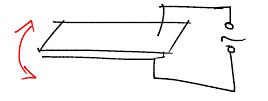
\includegraphics[scale=0.5]{fig5.png}
% \end{figure}

Sie Besitzen einen Gangungenauigkeit von $1$ s/Woche. Sie besitzen also einen Fehler von $1$s pro $10^6$s
\item Es gibt aber auch die Möglichkeit mittels atomarer Eigenschwingungen (atomare Uhren) die Zeit noch genauer zu messen.  Deren Ganggenauigkeit entspricht $1$ s/$3000$ Jahren. Dies findet unter anderem Anwendung im GPS. 
\item $\ce{^{133}Cs}$ Hyperfeinübergang

Es ergibt sich die Definition $1\s=9.192.631.770$-faches der Periodendauer des Hyperfeinübergangs in $\ce{^{133}Cs}$. Diese ist überall nachvollziehbar!
\item Zeitmessung durch radioaktiven Zerfall Kerne mit großer Masse $\rightarrow$ instabil $N=$ Zahl instabiler Kerne. \\

Es gilt die Proportionalität $\frac{dN(t)}{dt} \sim N(t) $, dabei zerfallen die Kerne unabhängig voneinander. ($\rightarrow$ \emph{Unabhängigkeit}) 

 \begin{equation*}
  \frac{dN}{dt}=-\lambda \cdot N(t), \qquad \lambda: \text{ Zerfallskonstanste}, \lambda>0
 \end{equation*}
 \begin{equation*}
  N(T)=N_0 \cdot e^{-\lambda t}, \qquad N_0:= N(0), [\lambda]=\frac{1}{s}
 \end{equation*}

  \begin{figure}[ht]
   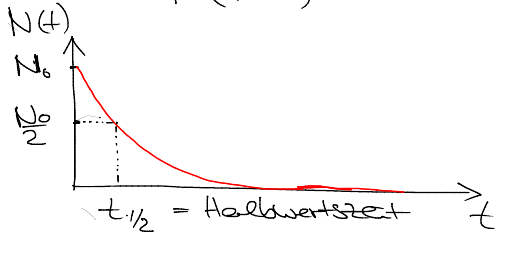
\includegraphics[scale=0.5]{bilder/fig6}
  \end{figure}

\begin{align*}
  \frac{N_0}{2} &= N_0 \cdot e^{-\lambda t_{\frac 1 2}}\\
  \ln 0.5 &=-\lambda \cdot t_{\frac 1 2} \\
  t_{\frac 1 2} &= - \frac{\ln 0.5}\lambda = {\ln 2}{\lambda} 
\end{align*}

 \begin{ex*}
  \begin{enumerate}[a)]
   \item $\ce{^{224}_{88} Tn} \rightarrow \ce{^{220}_{86} Ru} + \alpha, \qquad \alpha=\ce{^4_2 He}$ mit Halbwertszeit $t_{\frac 1 2}=556s$
   \item $\beta$-Zerfall: $\ce{^{14}_6 C} \to \ce{^{14}_7 N} + e^- \bar v_l$ mit Halbwertszeit $t_{\frac 1 2}=5730 a$  
 \end{enumerate}
 \end{ex*}
\item Radio-Carbon-Methode \\
 Kohlenstoff liegt in der Athmosphäre in den Isotopen $\ce{^{12}_6 C}, \ce{^{13}_6 C}, \ce{^{14}_6 C}$ vor.

\begin{table}
\centering
 \caption{Verteilung in Atmosphäre}
 \begin{tabular}{c|c}
  $\ce{^{12} C}$&  $98,89\%$ \\
  $\ce{^{13} C}$& $1,11\%$ \\
 $\ce{^{14} C}$& $10^-10 \%$ \\
 \end{tabular}
\end{table}
 Wobei erstere beiden stabil und $\ce{^{14} C}$ instabil ist.  Lebende Organismen besitzen aufgrund von Stoffaustausch identische Kohlenstoff-Verteilung.  Stirbt der Organismus verändert sich das Isotopenverhältnis.

 
 \begin{align*}
  \ce{^{14} C(t)}&=\ce{^{14} C_0} \cdot e^{-\lambda t} \\
 \ce{^{13} C(t)}&=\ce{^{12} C_0}\\
 \frac{\ce{^{14} C}}{\ce{^{12} C}} |_\text{Fossil} (t)&= \frac{\ce{^{14} C_0}}{\ce{^{12} C_0}} e^{-\lambda t}, \qquad \lambda=1.121\cdot 10^{-4} \frac{1}{a}
 \end{align*}
\item C14-Methode: experimentelle Bestimmung\\
Die Zerfalleigenschaft des $C-14$, lässt sich ausnutzen, um kleine Zeitmaße zu messen.
\begin{ex*}
 $\frac{\ce{^{14}  C}}{\ce{^{12} C}}$ im Fossil (Massenspektrum) $\rightarrow$ Alter $t \rightarrow$ Alter + Höhlenzeichnung in S-Frankreich:  $15.500$ Jahre
\end{ex*}
\end{itemize}
\end{Beispiel}





\subsection{L"ange}

\begin{Def}[Meter \textbf m]\index{Meter}\label{def_meter}
   $1m = c_0 \cdot \frac{1}{299\, 792\, 458}\operatorname{s}$ mit der
   (Vakuum)Lichtgeschwindigkeit $c_0$.
\end{Def}

Um \textbf{sehr gro"se} Abst"ande zu messen, benutzt man
Triangulationsverfahren. Bei \textbf{sehr kleinen} Abst"anden
Laserinterferomenter, bei denen man ausnutzt, dass sich Lichtwellen
bei bestimmten Bedingungen ausl"oschen und die Lichtwellenl"ange bekannt
ist.

\begin{table}[ht]
\centering
\caption{Größenordnung von Längen}
 \begin{tabular}{l r}
  Erde-Fixstern & $4\cdot 10^{16} \m$\\
  Erde-Sonne & $1.5 \cdot 10^{11} \m$\\
 Erdradius & $63 \cdot 10^6 \m $\\
 Sichtbares Licht (Wellenlänge) & $ 500\cdot 10^{-9}$m \\
 Atomdurchmesser & $10^{-10}$m  \\
 Kerndurchmesser & $10 ^{-15}$m
 \end{tabular}
 \end{table}
 \newpage
\begin{Beispiel}
\begin{itemize}
\item Geschichte des Meters:\\
1799 wurde der Meter definiert durch $1 \m \hat = \frac{1}{400000000}$ des durch Paris gehenden Großkreises ($40\cdot 10^3$ km). 1795 wurde ein Prototyp des Urmeters aus Messing hergestellt.

Einige Jahre später wurde der Urmeter aus Platin hergestellt und in einem Stahlschrank im französischen Nationalarchiv 1799 verschlossen. Heute wird es in einem Tresor des Internationalen Büros für Maße und Gewicht (BIPM) in S\`evres aufbewahrt.

1889 wurde das Urmeter von der Generalkonferenz für Maß und Gewicht durch das Urmeter einer Platinlegierung($90\% \ce{Pt}$ und $10\% \ce{Ir}$) ersetzt.

 Seit 1983 ist der Meter über den Lichtweg definiert:
 \[
  1\m=\text{ Länge des Weges Weges, den Licht im Vakuum in $\frac{1}{299792485} s$ zurücklegt.}
 \]

\item Messung von Abständen mittels Triangulation:\\
 \begin{figure}[!ht]
  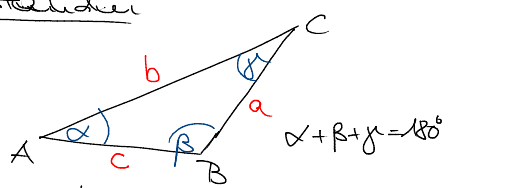
\includegraphics[scale=0.5]{bilder/fig7}
 \end{figure}
 Sinussatz: $\frac{c}{\sin\gamma} = \frac{a}{\sin{\beta}}=\frac{a}{\sin\alpha}$ \\
 
 \begin{itemize}
  \item $\alpha, \beta$ bekannt $\to \gamma$ bekannt
  \item $c$ bekannt, dann lässt sich $a$ bzw. $b$ berechnen zu:
\begin{align*}
a&=c\cdot \frac{\sin \alpha}{\sin \gamma}\\
b&=c\cdot \frac{\sin \beta}{\sin \gamma}
\end{align*}
 \end{itemize}
\newpage
\item Abstand-Erde-Mond \\
 \begin{figure}[!h]
  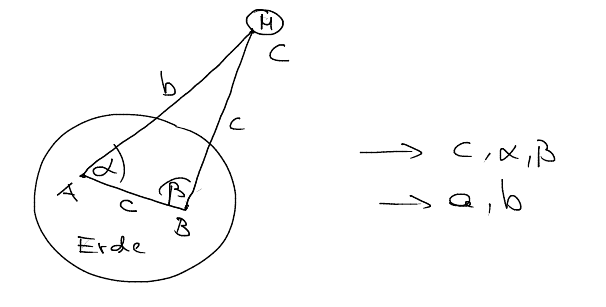
\includegraphics[scale=0.5]{bilder/fig8}
 \end{figure}

\item Abstand Erde-Sonne\\
 Als Basis (c) wähle Erde-Mond
 \begin{figure}[!h]
  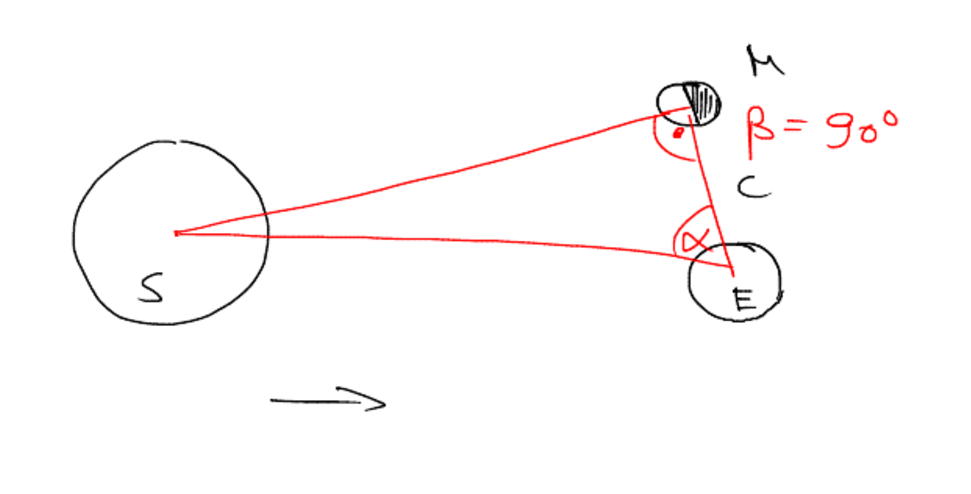
\includegraphics[scale=0.5]{bilder/fig9}
 \end{figure}
 Bei Halbmond besitzt $\beta=90^\circ$.  Den Abstand Erde-Mond lässt sich messen. Dann genügt es Den Winkel zwischen Mond und Sonne auf der Erde messen und damit ergibt sich der Abstand zum Mond.

\item LIDAR (Light Detection and raging)\\
 \begin{figure}[!h]
  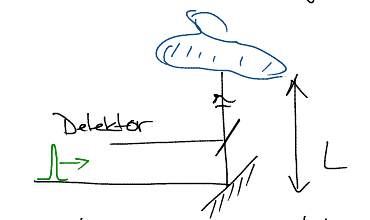
\includegraphics[scale=0.5]{bilder/fig10}
 \end{figure}
 \[
 T=\frac{2L}{c}
 \]
 
\item Messungen kleiner Entfernungen Laserinterferometer (\emph{Michelson-Interferometer})

%  \begin{figure}[ht]
%   \includegraphics[scale=0.7]{fig11}
%  \end{figure}

 \[
  \Delta s= 2 |s_1-s_2|
 \]

 Die Verschiebung um $\frac{20 \my m}{\text{64 Maxima}}=0.625 \to \lambda=630\my \m $
\end{itemize}
\end{Beispiel}




\subsection{Masse}

\begin{Def}[Kilogramm
   \textbf{Kg}]\index{Kilogramm}\label{def_kilogramm}
   $1Kg = \text{Masse des Urkilogramms}$. Das Urkilogramm ist ein
   Gewicht in Paris, welches das Kilogramm definiert.
\end{Def}

Das Kilogramm ist also eine \emph{willk"urliche} {Definition} und nicht
"uber Natukrkonstanten definiert. Man versucht hier Abhilfe zu
schaffen, indem man bspw. eine monokirstalline Siliciumkugel erstellt,
bei der man genau die Anzahl der Atome bestimmen kann, deren einzelnes
Gewicht bekannt ist -- so k"onnte man eine allgemeine, (unter gro"sem
Aufwand) reproduzierbaer Definition des Kilogramms erstellen.







\subsection{MKS-System}
\label{kap_mks-system}

\begin{Def}[MKS-System]\index{MKS-System}
   Ein \emph{Ma"ssystem}, welches alle in der \emph{Mechanik} wichtigen
   Einheiten auf die drei Grundeinheiten
   \begin{itemize}
   \item Meter
   \item Kilogramm
   \item Sekunde
   \end{itemize}
   zur"uckf"uhrt.
\end{Def}

\index{SI-System} Das \textbf{SI-System} (\emph{System
  Internationale}) stellt dar"uber hinaus weitere Einheiten zur
Verf"ugung, die Grundlage sind f"ur weitere Teilgebiete der Physik:

\begin{description}[\setlabelstyle{\bfseries\slshape}]
\item[Thermodynamik] Absolute Temperatur in Kelvin $\mathbf
   K$\\Stoffmenge in Mol $\mathbf{mol}$
     \item[Elektrodynamik] Stromst"arke in Ampere $\mathbf A$
     \item[Optik] Lichtst"arke in Candela $\mathbf{Cd}$
 \end{description}






\section{Messfehler}\index{Messfehler}

\subsection{Systematischer Messfehler}

\begin{Def}[Systematischer Messfehler]\index{Systematischer
     Messfehler}
     Als \emph{systematischer Fehler} (auch systematische Abweichung oder -Verzerrung; engl. systematic error oder bias) werden in der Technik, den Natur- und anderen Wissenschaften Messfehler bezeichnet, die sich bei wiederholter Messung nicht im Mittel aufheben. Diese Fehler sind prinzipiell vermeidbar.
\end{Def}

\textbf{Ursachen} k"onnen sein:
\begin{itemize}
     \item ein falsch geeichtes Messinstrument
     \item Nichtberücksichtigen von \emph{Konstanten} äußerer Einflüsse
     \item Rundungen / Vereinfachungen in den Formeln (zum Beispiel die Anwendung der Kleinwinkelnäherungen $ \sin \alpha \approx \alpha $ und $ \cos \alpha \approx 1 $
\end{itemize}




\subsection{Statistische (zuf"allige) Messfehler}

\begin{Def}[Statistische Messfehler]\index{Statistische Messfehler}
   Als \emph{zufällige Abweichungen} oder \emph{Zufallsfehler} werden die Abweichungen der Messwerte von ihrem Mittelwert bezeichnet. 
   Zufällige Abweichungen streuen in Betrag und Vorzeichen. Sie sind im Allgemeinen nicht vermeidbar.
\end{Def}

\textbf{Ursachen} k"onnen sein:
\begin{itemize}
     \item Ablesefehler durch Beobachter (wobei diese natürlich auch systematisch sein können, durchaus sind aber auch Streuungen beim Ablesen denkbar)
     \item (statistische) Schwankungen "au"serer Einfl"usse
\end{itemize}

Diese Fehler sind i.A. nicht vermeidbar, jedoch verringerbar. Man
bedient sich dazu statistischer
Auswertungsmethoden\index{Statistik}. Wiederholt man den Versuch oft,
kann man einen \textbf{Mittelwert}
\begin{equation}
     \bar x = \frac{1}{n} \cdot \sum_i x_i
\end{equation}
der $n$ Messwerte $x_i$ bestimmen. 

Weiter gibt die \textbf{Standardabweichung} oder \textbf{Streuung}
\begin{equation}
     \sigma = \sqrt{\frac{1}{n-1} \cdot \sum_i (x_i - \bar x )^2}
\end{equation}
an, wie zuverl"assig $\bar x$ ist -- Messwerte $x_i$ innerhalb der
$\sigma$-Umgebung von $\bar x$ treten mehr als halb so h"aufig auf, wie
$\bar x$ selbst.

Um die W"ahrscheinlichkeit $p$ zu berechnen, mit der ein bestimmter
Messwert $x$ auftreten sollte, verwendet man die
\textsc{Gauss}'sche-Normalverteilung\index{Normalverteilung}. Diese besitzt die Wahrscheinlichkeitsdichte:
\begin{equation}
   p(x) = \frac{1}{\sqrt{2\pi} \cdot \sigma} \cdot 
   \exp\left ( \frac{- (x-\bar x)^2}{2\sigma^2} \right )
\end{equation}
\fixme[Graph der Dichtefunktion fehlt]

Als Dichtefunktion besitzt $ p $ die Eigenschaft:
\[
P(]-\infty, \infty[)=\int_{-\infty}^{\infty} p(x)\, dx=1
\]
Die Wahrscheinlichkeit $P$, das x im Intervall $\bar x \pm \sigma$ streut ist damit. 
\[
\int\limits_{\bar x-\sigma}^{\bar x+\sigma} p(x)=0,683
\]
Man bezeichnet dies auch als \emph{statistische Sicherheit} bzw. \emph{Vertrauensgrenze} $P$ für $\delta=\sigma$.

\begin{table}[h]
\centering
\caption{Statistische Sicherheit bzw. Vertrauengrenze $P$ für $\delta$}
\begin{tabular}{c|c}
$\delta[\sigma]$ & $P=\int\limits_{\bar x-\delta}^{\bar x+\delta} p(x) dx$ \\ \hline
1 & 0,683 \\
0,676 & 0,5 \\
1,96 & 0,95 \\
3,0 & 0,997
\end{tabular}
\end{table}


\subsection{Exkurs: Wahrscheinlichkeitstheorie $ (\bigstar) $}
\begin{Def}[Wahrscheinlichkeitstheorie aus WIKIPEDIA]
Die Wahrscheinlichkeitstheorie oder Wahrscheinlichkeitsrechnung ist ein Teilgebiet der Mathematik, das aus der Formalisierung der Modellierung und der Untersuchung von Zufallsgeschehen hervorgegangen ist. Gemeinsam mit der mathematischen Statistik, die anhand von Beobachtungen zufälliger Vorgänge Aussagen über das zugrunde liegende Modell trifft, bildet sie das mathematische Teilgebiet der Stochastik. Die zentralen Objekte der Wahrscheinlichkeitstheorie sind zufällige Ereignisse, Zufallsvariablen und stochastische Prozesse.
\end{Def}
Im Folgenden möchten wir einige wahrscheinlichkeitstheoretische Begriffe kurz erklären. 
\begin{description}
\item[Wahrscheinlichkeit:] Die Wahrscheinlichkeit (Probabilität) ist eine Einstufung von Aussagen und Urteilen nach dem Grad der Gewissheit (Sicherheit). Im Zusammenhang mit der Maßtheorie bezeichnen wir ein Maß $ P $ als Wahrscheinlichkeitsmaß, ein Maß, dass in seiner Gesamtheit ihrer Ereignisse 1 ist.
\item[Maß:] Wir bezeichnen $ \my: C \to [0, \infty] $ mit $ A_i \in C $, wobei $ C $ die Menge der möglichen Ereignisse bezeichnet, als Maß falls gilt:
\begin{itemize}
\item $ \my(\emptyset)=0 $
\item  $ \sigma- $Additivität: $ \my\left ( \bigcup_{i\ge 1} A_i \right )= \sum_{i\ge 1} \my(A_i) $
\end{itemize}
\item[Verteilungsdichte:] Mittels der Verteilungsdichte $ f $ können wir die Wahrscheinlichkeit des Ereignisses berechnen durch:
\[
P([a,b])=\int_a^b f(x) \, dx
\]
Bestimmte Verteilungsarten (z.B.: unitäre (bedeutet: gleichverteilt) Verteilung, Normal-/GAUSS-Verteilung)
\item[Verteilungsfunktion:] Auch die Verteilungsdichte $ F $ ermöglicht uns die Berechnung der Wahrscheinlichkeit
\[
P([a,b])=F(b)-F(a)
\]
Die Verteilungsfunktion hat einige Grundlegende,  sie wächst monoton und ist rechtsseitig stetig. Dies liegt natürlich nahe, da es sonst negative Wahrscheinlichkeiten gäbe. Auch diese hängen von der Art der Verteilung (dies entspricht im Wesentliche die Art des Zufalls) ab.
\item[Zähldichte] Ist die Grundmenge der Ereignisse endlich, so bezeichnen wir den Wahrscheinlichkeitsraum als diskret (so zum Beispiel beim Münzwurf oder Würfel). In diesem Fall,  können wir für die Einzelergebnisse Wahrscheinlichkeiten angeben wir bezeichnen die Zugehörige Funktion $ f $ als Zähldichte. Es gilt:
\[
P(\{x\})=f(x)
\]
\item[Unabhängigkeit] Wir sagen zwei Ereignisse $ A, B $ sind unabhängig, wenn gilt:
\[
P(A\cap B)=P(A)\cdot P(B)
\]
Dies entspricht der Baumregel für diskrete Wahrscheinlichkeitsräume.  Also, sind Ereignisse unabhängig, wenn die Messungen nicht voneinander abhängen, also in keiner Relation zueinander sind. Ein Beispiel wäre das Würfeln mit zwei Würfeln. 
\end{description}

\begin{Wichtig}
Weder bedeutet Wahrscheinlichkeit 0, dass ein Ergebnis nicht eintreffen kann, noch sagt die Wahrscheinlichkeit 1, dass das Ergebnis stets eintrifft. Dies kann man sich daran verdeutlichen, dass es "`unendlich"' unwahrscheinlich, dass wenn man von einem Hochhaus einen Stein runterwirft, ihn exakt an einem gewissen Punkt wiederzufinden, jedoch kann tatsächlich jeder beliebige Punkt (zu mindest theoretisch) erreicht werden. Dagegen ist es "`unendlich"' wahrscheinlich, dass der Stein außerhalb des Punkts aufkommt, doch auch dies ist natürlich nicht notwendigerweise der Fall.  Für Wahrscheinlichkeit 1 sprechen wir von einer $ P $-fast sicheren Eigenschaft.  
\end{Wichtig}










\chapter{Kinematik}







\section{Eindimensionale Bewegung}
\label{kap_kinematik_eindimensional}
\index{eindimensionale Bewegung}

Also Bewegung l"angs einer geraden Linie.

Man unterscheidet zwischen der \textbf{Gleichf"ormigen
  Bewegung}\index{gleichf"ormige Bewegung} mit konstanter
Geschwindigkeit ($v = \frac{\Delta s}{\Delta t} = \frac{\diff x}{\diff
  t}= const$) und \textbf{nicht-gleichf"ormiger Bewegung}, bei der die
Geschwindigkeit eben \emph{nicht} konstant ist. Hier kann man die
mittlere Geschwindigkeit,
bzw. \textbf{Momentangeschwindigkeit}\index{Momentangeschwindigkeit}
\begin{equation}
     v = \frac{\diff s}{\diff t}
\end{equation}
bestimmen.\footnote{Man kann sagen, dass die Momentangeschwindigkeit
  auch eine gemittelte Geschwindigkeit ist, nur dass man das
  Zeitintervall $\Delta t$, "uber welchem man mittelt, sehr klein
  macht: $\Delta t \to 0$.} Bei dieser Bewegung handelt es sich um
eine \textbf{beschleunigte Bewegung}, wobei man die Beschleunigung
bestimmen kann:
\begin{equation}
\boxed{
     a = \frac{\diff v}{\diff t} = \frac{\diff^2 s}{\diff t^2}
}
\end{equation}



Um entsprechend aus einer gegebenen Beschleunigung $a(t)$ die
Momentangeschwindigkeit und die bisher zur"uckgelegte Strecke zu
berechnen, integriert man die Beschleunigung "uber die Zeit:
\begin{equation}
   v(t) = \int_0^t a(\hat t) \diff \hat t \text{ und } s(t) = 
   \int_0^t v(\hat t) \diff \hat t
\end{equation}
\begin{Wichtig}
   Wichtig ist dabei, dass man beim Integrieren auch sch"on brav die
   Integrationskonstanten mitnimmt -- sie stellen
   Anfangsgeschwindigkeit $v_0$ bzw. bereits zur"uckgelegte Strecke
   $s_0$ dar!
\end{Wichtig}







\section{R"aumliche Bewegung}
\index{R"aumliche Bewegung}


\begin{Def}[Trajektorie]\index{Trajektorie}
   Ist die Kurve im Raum, auf der sich ein (Massen)Punkt bewegt. Man
   bezeichnet sie oft mit $\gamma$ oder $\vec r(t)$
\end{Def}
Dabei ist $\gamma$ eine Funktion (oder
\emph{\index{Parametrisierung}Parametrisierung}) mit $\gamma : \mathbb
R \to \mathbb R^3: ~ t \mapsto \Ve r(t)$ -- und so wird $\vec r = \vec
r(t)$ auch Trajektorie genannt.

Bei Bewegungen im Raum kann man im Allgemeinen die Definitionen von
Kap. \ref{kap_kinematik_eindimensional} verwenden. Hier verwendet man
eben statt der einfachen Strecke $s$ die Raumkurve $\Ve r$.

\begin{Wichtig}[Ableiten von Vektoren]
   \index{Vektor!ableiten}\index{Ableiten von Vektoren} Man leitet
   einen Vektor ab, indem man die Komponenten ableitet:
     $$
      \Ve s = \begin{pmatrix}
                   x\\y\\z
              \end{pmatrix} ~ \Rightarrow ~
              \dot{\Ve{s}} = \begin{pmatrix}
                                  \dot x\\\dot y\\\dot z
                             \end{pmatrix}
     $$
\end{Wichtig}


Nun ist im noch zu beachten, dass die (r"aumliche) Geschwindigkeit $\Ve
v$ stets \emph{in Richtung der Bahntangente} zeigt, w"ahrend die
(r"aumliche) Beschleunigung $\Ve a$ im allgemeinen \emph{nicht in
  Richtung der Bahntangente} zeigt. D.h. $\Ve a$ kann sowohl
Komponenten in Richtung der Bahntangente haben (diese nennen wir $\Ve
a_T$), als auch senkrecht dazu (diese entsprechend $\Ve a_N$ -- das
"`$N$"' steht f"ur \emph{normal}).

Mathematisch kann man das herleiten, indem man die Geschwindigkeit $\Ve
v$ beschreibt als Skalar $v$ und Einheitsvektor $\Ve u_T$, der zur
Bahnkurve des Teilchens jeweils tangential steht:
$$
\Ve v = v \cdot \Ve u_T ~ \Rightarrow ~ \dot{\Ve{v}} = \Ve a =
\frac{\diff}{\diff t} (v \cdot \Ve u_T) = \underbrace{\frac{\diff
    v}{\diff t} \cdot \Ve u_T}_{\Ve a_T} + \underbrace{v \cdot
  \frac{\diff \Ve u_T}{\diff t}}_{\Ve a_N}
$$

Nun muss man untersuchen, wie $\frac{\diff \Ve u_T}{\diff t}$ aussieht. 
Dazu unterscheidet man zwei Spezialf"alle:

\begin{description}[\setlabelstyle{\bfseries\slshape}]
\item[Geradlinige Bahn] dann ist $\frac{\diff \Ve u_T}{\diff t} = 0$
   da $\Ve u_T = const$. Dann haben $\Ve v$ und $\Ve a$ die selbe
   Richtung -- und man ist wieder beim eindimensionalen Fall wie in
   Kap \ref{kap_kinematik_eindimensional} gelandet.
\item[Gekr"ummte Bahn] Hier n"ahert man die Kr"ummung durch einen Kreis
   an. Hier zeigt die Ableitung der Tangente radial zum
   Kreismittelpunkt -- also senkrecht zur Tantente. So ergibt sich
   also eine Komponente $\Ve a_N \neq \Ve 0$.
\end{description}








\section{Superpositionsprinzip}
\index{Superposition}


\begin{Def}[Superpositionsprinzip]
   Diese Prinzip besagt, dass man eine Bewegung in unabh"angige
   Teilbewegungen zerlegen kann.
\end{Def}

So wird beispielsweise ein \textbf{Schiefer Wurf} zerlegt in eine
(nach unten) beschleunigte Bewegung und eine gleichf"ormige Bewegung in
der Horizontalen.

Das Superpositionsprinzip ist immer (im Sinne von "`genau dann wenn"')
bei \emph{\index{Lineare Theorie}Linearen Theorien} anwendbar.




\section{Kreisbewegung I}
\label{kap_kreisbewegung-i}
\index{Kreisbewegung}

Wir betrachten hier eine gleichf"ormige Kreisbewegung (mit Radius $R$),
d.h. dass die Winkelgeschwindigkeit $\omega = \dot \varphi$ ($\varphi$
ist der im Kreis "uberstrichene Winkel im Bogenma"s) konstant ist. Dabei
wird $\omega$ auch als Vektor interpretiert: Er steht senkrecht auf
der Kreisbewegung und folgt der \textbf{Rechten Faust Regel}: D.h. 
die Finger der rechten Faust zeigen in die Richtung, in die das
Massenteilchen rotiert, dann zeigt der ausgestreckt Daumen in die
Richtung des Vektors $\Ve \omega$.

Man kann die Bahnkurve eines solchen Teilchens parametrisieren durch
$$
 \Ve r = \begin{pmatrix}
              R \cdot \cos \varphi(t)\\
              R \cdot \sin \varphi(t)
         \end{pmatrix}
$$

Das Bogenma"s eines Winkels ist definiert als
\begin{equation*}
   \varphi = \frac{s}{r}
\end{equation*}
wobei $r$ der Radius und $s$ die \emph{Kreisbogenl"ange} eines
Kreisbogens ist, der den "Offnungswinkel $\varphi$ bestitzt. F"ur eine
Rotation um einen konstanten Radius $r$ ist deswegen die
\index{Winkelgeschwindigkeit}\textbf{Winkelgeschwindigkeit}:
\begin{equation}
   \label{eqn_winkelgeschwindigkeit_kreis}
   \omega = \dot \varphi = \frac{\dot s}{r} = \frac{v}{r}
\end{equation}
Wenn wir nun einen \emph{Vektor} $\vec v$ untersuchen, so sehen wir,
dass dieser seine Richtung st"andig "andert -- weil $v = \omega \cdot r$
ist, und $\omega$ und $r$ konstant sind, ist die \emph{L"ange} des
Vektors jedoch konstant. 

Untersucht man den Geschwindigkeitsvektor
eines mit $\omega = \const$ rotierenden Teilchens zu zwei Zeiten, so
ist der Winkel $\diff \varphi$ nicht nur der "Offnungswinkel zwischen den
beiden Ansatzpunkten der Vektoren, sondern auch der Winkel zwischen
den Vektoren. "Uberlegt man weiter, dass die Vektorspitze demnach einen
Kreisbogen der L"ange
\begin{equation*}
   \| \diff \vec v \| = v \cdot \diff \varphi
\end{equation*}
zur"uckgelegt hat, so findet man, in dem man
\eqref{eqn_winkelgeschwindigkeit_kreis} nach $v$ aufl"ost, einsetzt und
durch $\diff t$ teilt:
\begin{equation}
   \label{eqn_winkelbeschleunigung_kreis}
\left \|   \frac{\diff }{\diff t} \vec v \right \| =  \dot \varphi r
\cdot \frac{\diff \varphi}{\diff t} = {\dot \varphi}^2 r = \omega^2
\cdot r = a_Z
\end{equation}
Man erh"alt also die
\textbf{\index{Zentripetalbeschleunigung}Zentripetalbeschleunigung}.
Multipliziert man diese nun mit $m$ erh"alt man wegen $F = ma$ die
Zentripetalkraft zu
\begin{equation}
   \label{eqn_zentripetalkraft_kreis}
   F_z = m \cdot \omega^2 \cdot r
\end{equation}



Bei der Kreisbewegung ergeben sich nun folgende Gr"o"sen:
\begin{description}[\setlabelstyle{\bfseries\slshape}]
     \item[Periodendauer] $T = \frac{2\pi}{\omega}$
     \item[Frequenz] $f = \nu = \frac{1}{T} = \frac{\omega}{2\pi}$
     \item[Bahngeschwindigkeit] $\boxed{v = \frac{2\pi R}{T} = \omega \cdot R}$
bzw. $\vec v =  \vec \omega \times \vec r$
     \item[Zentripetalbeschleunigung] $\Ve a_Z = \frac{v^2}{R} \cdot
        \Ve u_N ~\Rightarrow ~ \boxed{\|\Ve a_Z\| = \omega^2 \cdot R}$
        \\gilt nur f"ur $\omega = const$!
 \end{description}


\begin{Wichtig}[$\nu \neq v$]
   Der griechische Buchstabe $\nu$ ("`n"u"') gibt meistens Frequenzen
   an, w"arend das lateinische $v$ ("`vau"') oft f"ur Geschwindigkeiten
   verwendet wird. Nicht verwechseln!
\end{Wichtig}

















\chapter{Mechanik eines einzelnen Massenpunktes}



\section{Schwere Masse und Tr"age Masse}

Grunds"atzlich muss man zwischen zwei verschiedenen Arten von Masse
unterscheiden:

\begin{description}[\setlabelstyle{\bfseries\slshape}]
\item[{Schwere Masse} $m_G$] Durch bspw. eine Balkenwaage vergleicht
   man die Masse des zu wiegenden St"ucks mit einer Referenzmasse --
   bspw. dem Urkilogramm (s. Def. \ref{def_kilogramm} auf
   S. \pageref{def_kilogramm}). Beide Massen befinden sich im gleichen
   Schwerefeld.

\item[{Tr"age Masse} $m_T$] Das Massenteil wird bspw. zwischen zwei
   Federn eingespannt und zu Schwingungen angeregt. Es gilt $T \sim
   \sqrt{m_T}$ mit der tr"agen Masse $m_T$ und der Periodendauer
   $T$. Nun vergleicht man die Periodendauer einer Masse in diesem
   Aufbau mit der Periodendauer bspw. des Urkilogramms.
\end{description}
Die beiden Messmethoden verwenden zum Vergleich verschiedene
Eigenschaften des K"orpers. Mathematisch nicht zu beweisen, jedoch
durch zahlreiche Experimente untermauert ist nun die Formel
$$
\boxed{m_T = m_G = m}
$$
Dieser Zusammenhang wird auch \textbf{"Aquivalenzprinzip} genannt.

Man kann sogar sagen, dass die
\index{Gravitationskonstante}Gravitationskonstante $\gamma$ (auch $G$
genannt) so gew"ahlt wurde, dass f"ur die Zahlenwerte $m_T = m_G$
gilt.




\section{Kraft}

Kraft ist ein Vektor! Sie wird gemessen, indem man bspw. die
Verformung eines K"orpers betrachtet, an den diese Kraft angreift. Zwei
Kr"afte sind gleich, wenn sie die gleiche Richtung haben und wenn
sie bei dem K"orper die gleiche Verformung erwirken (also gleichen
\emph{Betrag} haben).








\section{Das \textsc{Newton}'sche Grundgesetz}\index{Newton}
\label{kap_newton}


\begin{Wichtig}[Tr"agheitsgesetz (I. \textsc{Newton}'sches Axiom)]
   \index{Newton I} Ein K"orper verharrt in Ruhe oder in
   gleichf"ormiger Bewegung wenn keine Kraft an ihn angreift.
\end{Wichtig}

\begin{Wichtig}[II. \textsc{Newton}'sches Axiom]\index{Newton
     II}
   Wenn ein K"orper beschleunigt werden soll, muss eine Kraft auf ihn
   einwirken.
\end{Wichtig}

Aus Experimenten ergibt sich, dass $a \sim F$ und $a \sim
\frac{1}{m}$. Kombiniert man diese beiden Formeln, so ergibt sich
$$
a \sim \frac{F}{m} ~\Rightarrow ~ F \sim m \cdot a
$$
Nun w"ahlt man die Krafteinheiten so, dass die
Proportionalit"atskonstante der Formel $1$ wird und schon hat man die
Ber"uhmte Formel von \textsc{Newton}:
\begin{Wichtig}[\textsc{Newton}'sche Grundgleichung]
\index{Newton'sche
     Grungleichung}\index{Newton II!Gleichung}
     \begin{equation}
          \boxed{
              F = m \cdot a
          }
          \label{eqn_newton}
     \end{equation}
\end{Wichtig}
bzw. mit Vektoren:
$$
\vec F = m \cdot \vec a
$$
und au"serdem hat man die Einheit der Kraft definiert:
\begin{Def}[Newton $\mathbf N$]\index{Newton (Einheit)}
     $1N = 1\frac{Kg \cdot m}{s^2}$
     
     Ein Newton ist die Kraft, die auf einen K"orper mit der Masse $1
     Kg$ wirken muss, damit dieser die Beschleunigung von $1
     \frac{m}{s^2}$ erf"ahrt.
\end{Def}
Damit ist die Einheit $N$ offensichtlich im MKS-System
(s. Kap. \ref{kap_mks-system}).


K"orper auf der Erde erfahren abh"angig von ihrer Masse eine Kraft in
Richtung des Erdmittelpunktes. Diese Kraft wird \textbf{Schwerkraft}
genannt. Nach der oben gefundenen Formel \ref{eqn_newton} entspricht
diese Kraft einer Beschleunigung in Richtung des Erdmittelpunktes. Wir
bemerken diese, wenn ein K"orper f"allt.
\begin{Def}[Erdbeschleunigung $\mathbf g$]
   Ein K"orper in der N"ahe der Erdoberfl"ache wird mit der
   Beschleunigung $g$ in Richtung des Erdmittelpunktes
   beschleunigt. Dabei ist $g$ von der Masse der K"orper unabh"angig!
     
   Man kann rechnen $F_g = m \cdot g$ und hat mit $F_g$ die
   \textbf{Gewichtskraft}, die auf einen K"orper wirkt. \footnote{Diese
     \emph{Linearisierung} der Erdanziehungskraft ist eigentlich nur
     eine N"aherung: Entfernt man sich weiter vom Erdboden oder begibt
     sich darunter, wird die Formel immer ungenauer. Siehe dazu
     Kap. \ref{kap_schwerkraft}.}
\end{Def}



\begin{Wichtig}[actio = reactio (III. \textsc{Newton}'sches
   Axiom)]\index{Actio}\index{Reactio}\index{Newton III}
   "Ubt ein K"orper $A$ eine Kraft $F_A$ auf den K"orper $B$ aus, so "ubt
   gleichzeitig $B$ auf $A$ eine Kraft $F_B$ aus. Die beiden Kr"afte
   haben dabei den gleichen Betrag und entgegengesetzte Richtungen,
   greifen jedoch an \emph{verschiedenen} K"orpern an!\footnote{Es
     handelt sich also nicht um ein Kr"aftegleichgewicht!}
     \begin{equation}
          \boxed{actio = reactio}
         \label{eqn_actio-reactio}
     \end{equation}
\end{Wichtig}






\subsection{Verschiedene Arten von Kr"aften}
\label{kap_arten_von_kraeften}

Wir unterscheiden im Allgemeinen zwischen

\begin{description}[\setlabelstyle{\bfseries\slshape}]
\item[Gewichts-/Schwerkraft]  Siehe Kap. \ref{kap_schwerkraft}
\item[Reibunsgkr"afte] \index{Reibungskraft}
Sie wirken entgegengesetzt der Bewegungsrichtung $\Vec v$.

   Mikroskopische Ursache sind kleinste Unebenheiten in K"orpern, die
   sich verzahnen und bei Bewegung muss diese Verzahnung "uberwunden
   werden. Ruht der K"orper, muss man
   \textbf{Haftreibung}\index{Haftreibung} "uberwinden, gleitet er
   \textbf{Gleitreibung}\index{Gleitreibung} und rollt er
   \textbf{Rollreibung}\index{Rollreibung}.

   All diese Reibungen sind innerhalb bestimmter Grenzen von der
   Geschwindigkeit unabh"angig zur Normalkraft $F_N$, mit der sie
   \emph{senkrecht} auf die Oberfl"ache gedr"uckt werden, proportional:
\begin{equation}
   \label{eqn_reibung}
   F_R = \mu \cdot F_N
\end{equation}
dabei ist $\mu$ der entsprechende Reibungskoeffizient und eine
Materealkonstante und unabh"angig von der Auflagefl"ache der K"orpers.
\item[Zentripetalkraft] Sorgt daf"ur, dass ein K"orper auf seiner
   Kreisbahn bleibt.

   Siehe Kap. \ref{kap_kreisbewegung-i}
\item[Federkraft] Es gilt das 
   \begin{Def}[\textsc{Hook}'sche Gesetz]
\index{Hook'sches Gesetz}\label{def_hook-sches-gesetz}
      Die L"ange $x$, um die eine Feder verformt wird, ist proportional
      zur ben"otigten Kraft $F_D$:
      \begin{equation}
         \label{eqn_hooksches-gesetz}
         F_D = - D \cdot x
      \end{equation}
      mit der \textbf{Federkonstanten} $D$ ($[D] = \frac{N}{m}$)
   \end{Def}
\item[Scheinkr"afte] Siehe Kap. \ref{kap_scheinkraefte}
\end{description}










\section{Schwerkraft}
\index{Schwerkraft}\label{kap_schwerkraft}


\begin{Def}[Schwerkraft]\label{def_schwerkraft}\label{def_gravitation}
     Die Schwerkraft ist eine von vier fundamentalen Kr"aften in der Physik! 
     
     Zwischen zwei K"orpern mit Masse besteht eine Anziehung -- diese
     wird \textbf{Schwerkraft} genannt.
\end{Def}

F"allt ein K"orper (oBdA ein Apfel) auf die Erde, so tut er das, weil
er von der Erde eine Kraft -- eben $F_g$ -- erf"ahrt und so in
Richtung der Erde beschleunigt wird. Gleichzeitig erf"ahrt die Erde
aber auch eine Kraft in Richtung Apfel. Wegen $actio = reactio$ gilt
nun
$$
F_1 = F_2 ~ \Leftrightarrow ~ m_A \cdot a_A = m_E \cdot a_E
$$
Nun ist aber $m_E \gg m_A$ und damit $a_A \gg a_E$. D.h. die Erde
f"allt auch -- nur sehr wenig.




\subsection{Messung von Schwerkraft -- Gravitationswaage}

In Abb. \ref{img_schwerkraftwaage} ist eine Skizze einer
\textbf{Gravitationswaage}. Hier l"asst man die beiden gro"sen Massen
$M$ zuerst weg und schaltet den Laser ein. Wenn man die Massen $M$
dann zugibt, werden die kleinen Kugeln $m$ von ihnen angezogen und die
ganze aufgeh"angte Apparatur dreht sich -- eben auch der Spiegel. So
wird der Laserstrahl abgelenkt. "Uber den Winkel kann man das
Drehmoment der Bewegung bestimmen -- und dadurch die Anziehungskraft
zwischen $m$ und $M$.

\begin{figure}
     \centering
     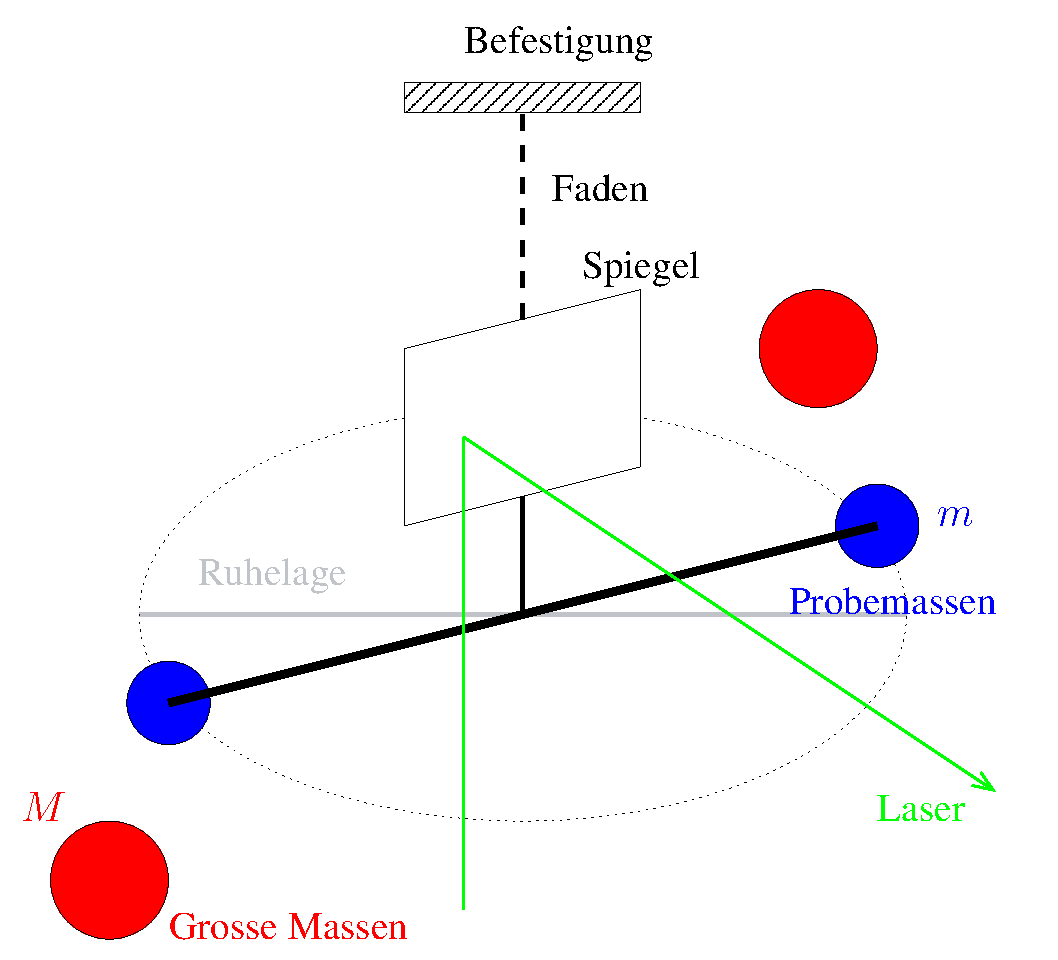
\includegraphics[width=0.7\textwidth]{bilder/gravitationswaage02}
     \caption[Gravitationswaage]{Die Massen $M$ lenken die Massen $m$
       ab, diese Drehen den Spiegel und ein Laserstrahl wird abgelenkt
% A: Aufh"angung, darunter der Faden. S: Spiegel; am Faden
%        befestigt. m: kleine Massen -- durch ein Gest"ange am Faden
%        befestigt. M: gro"se Massen, feste Positionen. 
}
     \label{img_schwerkraftwaage}
\end{figure}





\subsection{Berechnung der Schwerkraft}
\label{kap_scherkraft_berechnung}


Die Gravitationskraft zwischen zwei K"orpern kann man berechnen mit 
\begin{equation}
   \label{eqn_gravitation}
   \boxed{
      F = \gamma \cdot \frac{m_1 \cdot m_2}{r^2}
   }
\end{equation}
Dabei ist $r$ der Abstand zwischen den Massen $m_1$ und $m_2$ und $\gamma$ die
\begin{Def}[Gravitationskonstante $\gamma$ oder $G$]
\index{Gravitationkonstante}\label{def_gravitationskonstante}
   Die \textbf{Gravitationskonstante} ist eine Naturkonstante. Sie
   betr"agt
$$
 \gamma = 6,67 \cdot 10^{-11} \frac{m^3}{kg \cdot s^2}
$$
\end{Def}
Hieraus kann man auch einfach die Erdbeschleunigung berechnen:
$$
  F_G = m \cdot \underbrace{\frac{m_\text{Erde} \cdot \gamma}{r_E^2}}_g
$$
Hier kann man sehen, dass dies nur eine N"aherung ist, wenn
ein K"orper sich weiter von der Erdoberfl"ache entfernt.



\section{Scheinkr"afte}
\label{kap_scheinkraefte}

\begin{Def}[Inertialsystem]
\index{Inertialsystem}\label{def_inertialsystem}
Es treten nur dann Beschleunigungen auf, wenn Kr"afte wirken
\end{Def}

Man befindet sich dagegen in \emph{keinem} Inertialsystem, sondern in
einem \textbf{beschleunigten Bezugssytem}, wenn die
\emph{Newton}'schen Axiome scheinbar verletzt werden. 

Wird ein Wagen beschleunigt, so sind die K"orper darin tr"age und wollen
auf der Stelle verharren -- so sieht es ein Au"senstehender. Ein
Mitbewegter dagegen denkt, die K"orper w"urden sich bewegen -- also muss
auf sie eine Kraft wirken. Diese Kraft ist eine
\textbf{Scheinkraft}. Der Mitbewegte kann dabei nicht erkennen, woher
diese Kraft kommt. Der Mitbewegte befindet sich also \emph{nicht} in
einem Inertialsystem.


\abs
Wir untersuchen als Spezialfall ein \textbf{Rotierendes System:}

\begin{Wichtig}[Rotierender Vektor]
\index{rotierender Vektor}
   Rotiert ein Vektor $\Vec r = \vec r(t)$ mit $\Vec \omega = \vec \omega(t)$, so gilt
   \begin{equation}
      \label{eq:425}
      \boxed{
\frac{\diff \Vec r}{\diff t} = \vec v = \Vec \omega \times \Vec r
}
   \end{equation}
Mit der \textbf{Rechten-Hand-Regel} gilt also: $\Vec \omega$: Daumen,
$\Vec r$: Zeigefinger, $\frac{\diff \Vec r}{\diff t}$: Mittelfinger.
\end{Wichtig}

% Hat man also ein um $\Vec \omega$ rotierendes System $S'$ und ein
% ruhendes System $S$, in denen sich ein Vektor $\Vec r$ bewegt, so
% beschreibt man diese Bewegung in $S'$ durch
% $$
%  \frac{\diff \Vec r^*}{\diff t} = \Vec v - \Vec \omega \times \Vec r 
% = \frac{\diff \Vec r}{\diff t} - \Vec \omega \times \Vec r \textcolor{red}{\text{ist das dann nicht =0?}}
% ~
%  \text{ bzw. } ~ 
%  \frac{\diff \Vec v^*}{\diff t} = \Vec a - \Vec \omega \times \Vec v = 
% \frac{\diff v}{\diff t} - \Vec \omega \times \Vec v
% $$
% wobei $\Vec v$ im System $S$ beschrieben ist und durch $\Vec \omega
% \times \Vec r$ noch die Rotation von $S'$ ausgeglichen
% wird\footnote{Bewegt sich bspw. ein K"orper mit der Rotation von $S'$,
%   so sind die Zahlen, die seine Position in $S'$ beschreiben
%   \emph{kleiner} als die in $S$ -- deshalb muss man hier die Rotation
%   abziehen.} -- als Ergebnis hat man die Bewegung in $S'$
% beschrieben.

% M"ochte man nun die Kr"afte auf ein Massenteilchen in $S$ und in $S'$
% beschreiben, so erh"alt man wegen $\Vec r' = \Vec r$ den Zusammenhang
% $$
%  \Vec  F' = m \cdot \Vec a + 2 m \cdot ( \Vec \omega \times \vec V ) + m
%   \cdot \Vec \omega \times ( \Vec \omega \times \Vec r )
% $$
% \textcolor{red}{\text{warum ist hier $\Vec r' = \Vec r$, was ist $\Vec V ?$}}
% Es wirkt ja eigentlich nur die Kraft $\Vec F = m \cdot \Vec
% a$. D.h. der restliche Term muss den Scheinkr"aften zugeordnet
% werden. Man nennt sie 

Wir wollen nun einen Vektor $\vec R$ betrachten; er kann ruhen oder
sich bewegen. Diesen Vektor $\vec R$ stellen wir nun mithilfe zweier
Koordinatensystemen $S$ und $S'$ dar, wobei $S'$ konstant mit $\vec
\omega$ rotiert und $S$ in Ruhe ist.

Wir nennen die Basisvektoren in $S$ $e_i$ und die Basisvektoren in
$S'$ hei"sen $\varepsilon_i$ (auf Vektorpfeile wollen wir hier
ausnamsweise der "Ubersichtlichkeit halber verzichten); die
Koeffizienten in $S$ entsprechend $x^i$ und die in $S'$ hei"sen
$\xi^i$. Damit k"onenn wir den Vektor $\vec R$ in den beiden Systemen
schreiben als
\begin{equation*}
   \vec R = \sum_i x^i e_i \text{ und } \vec R = \sum_i \xi^i\varepsilon_i
\end{equation*}
Nun wollen wir die Ableitung von $\vec R$ betrachten und wenden dabei
die \emph{Produktregel} zum Ableiten an.

In $S$ beachtet man dabei, dass die $e_i$ ruhen, also dass $\dot e_i = 0$.
\begin{equation*}
   \frac{\diff }{\diff t}\vec R = \sum_i \dot x^i e_i + x^i \dot e_i =
   \sum_i \dot x^i e_i
\end{equation*}
In $S'$ gilt dies dagegen nicht. Daf"ur k"onnen wir mit
Gl. \eqref{eq:425} $\dot \varepsilon_i = \omega \times \varepsilon_i$
schreiben:
\begin{equation*}
   \frac{\diff }{\diff t} \vec R = \sum_i \dot \xi^i \varepsilon_i +
   \xi^i \dot \varepsilon_i = 
\sum_i \dot \xi^i \varepsilon_i +
   \xi^i \omega \times \varepsilon_i =
\sum_i \dot \xi^i \varepsilon_i +
    \omega \times (\xi^i \varepsilon_i )
\end{equation*}
F"ur die zweite Ableitung gilt entsprechend:
\begin{equation*}
   \frac{\diff ^2}{\diff t^2} \vec R = \sum_i \ddot x^i e_i
\end{equation*}
und im System $S'$ (hier verwenden wir, dass $\frac{\diff }{\diff t}
\omega = 0$ ist):
\begin{equation*}
     \frac{\diff ^2}{\diff t^2} \vec R =
\sum_i \ddot \xi^i\varepsilon_i + 2 \cdot \dot \xi^i \dot \varepsilon_i +
\xi^i\ddot \varepsilon_i =
\sum_i \ddot \xi^i\varepsilon_i + 2 \cdot \omega \times (\dot \xi^i  \varepsilon_i) +
\omega \times (\omega \times (\xi^i \varepsilon_i ))
\end{equation*}

Verwenden wir nun noch die Schreibweise $\vec x = \sum_i x^ie_i$ und
$\vec \xi = \sum_i \xi^i \varepsilon_i$ erhalten wir f"ur die
Beschleunigung von $\vec R$:
\begin{equation}
   \label{eq:426}
   \frac{\diff ^2}{\diff t^2} \vec R = \ddot{ \vec x} = \ddot{\vec
     \xi} + 2 \cdot \vec \omega \times \dot{\vec \xi} + \vec \omega \times (
   \vec \omega \times \vec \xi)
\end{equation}
D.h. die \emph{Kraft}, die im System $S$ zu sp"uren ist, ist schlicht
$ m \cdot \ddot{\vec x}$. Im System $S'$ aber:
\begin{equation}
   \label{eq:427}
   \vec F' = m \cdot  \ddot{\vec \xi} = m \cdot \left (\ddot{\vec x} -   2 \cdot \vec \omega \times \dot{\vec \xi} - \vec \omega \times (
   \vec \omega \times \vec \xi) \right )
\end{equation}
D.h. im beschleunigten System nimmt man mehr Kr"afte wahr, als im
ruhenden System. Man unterscheidet:


\begin{description}
\item[Corioliskraft]
\index{Corioliskraft}
\begin{equation}
   \label{eqn_coriolis-kraft}
\boxed{   \Vec F_C = -2 m \cdot ( \Vec \omega \times \vec v ) }
\end{equation}
Sie tritt auf, wenn ein K"orper sich senkrecht zur Rotationsrichtung
eines (mit Drehfrequenz $\Vec \omega$) rotierenden Systems
bewegt, also wenn $\vec \omega \times \vec v \neq 0$ ist. Dazu muss
$\vec \omega$ nicht konstant sein!

Bewegt sich bspw. ein K"orper (von au"sen beobachtet) gerade auf einer
rotierenden Scheibe nach au"sen, legt er (f"ur den Mitrotierenden)
au"sen an der Scheibe eine weitere Strecke seitw"arts als in der
Scheibenmitte zur"uck. Er muss also durch eine (Schein-)kraft seitlich
beschleunigt worden sein; der Corioliskraft. 


\item[Zentrifugalkraft]\index{Zentrifugalkraft} oder
   \textbf{Fliehkraft}\index{Fliehkraft}
\begin{equation}
   \label{eqn_zentrifugalkraft}
 \boxed{   -m\Vec \omega \times ( \Vec \omega \times \Vec r ) }
\end{equation}
Sie tritt in jedem rotierenden System auf und ist die (Schein-)Kraft, die
der Mitrotierende daf"ur verantwortlich macht, dass die Dinge nach
au"sen gezogen werden, obwohl diese ja eigentlich nur tangential nach
au"sen wegfliegen wollen. Sie ist vom Betrag her gleich der
Zentri\emph{petal}kraft, also der Kraft, die einen K"orper auf einer
Kreisbahn h"alt (s. \ref{kap_kreisbewegung-i}). Man kann sagen, dass
die Zentrifugalkraft die Reaktio der Zentripetalkraft ist.
\end{description}










\section{Energieerhaltungss"atze}
\label{kap_energieerhaltungssaetze}


\begin{Def}[Arbeit]
   \index{Arbeit}\label{def_arbeit}
Es wird die \textbf{Arbeit} $W$ verrichtet, um einen K"orper gegen die
Kraft $\Vec F(\Vec r)$ auf der Bahn $\Vec r(t)$ (mit der L"ange $s$ zwischen
Startpunkt $a$ und Endpunkt $e$) zu
bewegen:
\begin{equation}
   \label{eqn_def_arbeit}
   W  = \int_a^e \Vec F(\Vec r) \, \diff \Vec r
\end{equation}
\end{Def}
Die Einheit der Arbeit ist $[W] = J = N \cdot m = W \cdot s$

Eine Anschauliche Folgerung hieraus: \textbf{Das goldene Gesetz der
  Mechanik}
\begin{quote}
   Man braucht die gleiche Energie, um einen K"orper die Strecke $s$
   mit der Kraft $F$ zu bewegen, wie wenn man den K"orper doppelt so
   weit mit der halben Kraft bewegt
\end{quote}
(um $n \cdot s$ mit der Kraft $\frac{1}{n} \cdot F$ bewegt).



\begin{Def}[Konservative Kraft]
\index{Konservative Kraft}\label{def_konservative-kraft}
   Die zu verrichtende Arbeit h"angt nur vom Anfang und Ende der
   Bewegung ab -- nicht vom \emph{Weg}. 

   Rein Mathematisch kann man sagen, dass in diesem konservativen Kraftfeld die
   \textbf{Rotation verschwindet}: $\vec \nabla \times \Vec F(\Vec r) = 0$,
   bzw. dass jedes geschlossene Integral verschwindet (wenn man eine
   geschlossene Bahn f"ahrt, braucht man dazu insgesamt keine Arbeit):
   $\oint_\gamma \Vec F(\Vec r) \, \diff \Vec r = 0$
\end{Def}

Wird nun Arbeit entgegen einer konservativen Kraft verrichtet, so ist
die Arbeit in Form von \textbf{Potentieller Energie}\index{Potentielle
Energie} gespeichert. Man spricht dann auch davon, dass ein Teilchen,
welches man mit der Arbeit $W$ im konservativen Kraftfeld $F$ bewegt
hat, das \textbf{Potential} 
\begin{equation}
   \label{eqn_potential}
     E_{pot} = -W
\end{equation}
besitzt.
\emph{Beispiele} f"ur solche konservativen Kr"afte sind
\begin{itemize}
\item Schwerkraft
\item Elastische Federkraft
\end{itemize}
und \emph{Gegenbeispiele} sind
\begin{itemize}
\item Reibungskraft (Wegabh"angig)
\item \textsc{Lorentz}kraft (Geschwindigkeitsabh"angig)
\end{itemize}
Hier kann man auch sehen, dass bei einer nicht konservativen Kraft
die Arbeit sp"ater nicht mehr zur Verf"ugung steht.

\begin{Def}[Potenzielle Energie]
   \index{Potentielle Energie}\label{def_potentielle_energie} 
   Um die Potentielle Energie eines Teilchens in einem Kraftfeld
   allgemein zu bestimmen, ben"otigt man einen festen Bezugspunkt
   $P_0$. Nun gilt f"ur das Potential an einem Ort $Q$:
\begin{equation}
   \label{eqn_potential_allgemein}
   \boxed{E_{pot} = - \int_{P_0}^Q \Vec F(\Vec r) \, \diff \Vec r}
\end{equation}   
\end{Def}

Ein Teilchen wird sich in der Natur stets so bewegen, dass es
potentielle Energie abgibt; es strebt ein (potentielles)
\emph{Energieminimum}\index{Energieminimum} an. Es wird sich so stets
dorthin bewegen, wo die "Anderung des Potentials am st"arksten negativ
ist(wo die Abnahme des Potentials maximal ist).
Dies interpretieren wir als \emph{Kraft}.

Mathematisch kann man das auch so ausdr"ucken:
\begin{equation}
   \label{eqn_gradientenfeld}
   \Vec F = - \Grad E_{pot} = - \nabla E_{pot}
\end{equation}

Und auch die Umkehr gilt: Kann man ein Kraftfeld als Gradientenfeld
ausdr"ucken (kann man also Gl. \eqref{eqn_gradientenfeld} f"ur dieses
Kraftfeld aufstellen), so handelt es sich um eine konservative Kraft.



\begin{Wichtig}["Aquipotentialfl"achen]
\index{"Aquipotentialfl"achen}\label{def_aequipotentialflaechen}
In einem konservativen Kraftfeld findet man Stellen, an denen die
Potentielle Energie gleich ist. Diese Stellen kann man mit Linien verbinden und sie
bilden so eine Fl"ache. Innerhalb dieser Fl"ache kann man K"orper ohne
Arbeitsaufwand bewegen.   
\end{Wichtig}

Im Schwerefeld der Erde bspw. sind die "Aquipotentialf"achen
Kugelschalen mit dem Erdmittelpunkt im Zentrum. Anschaulich hei"st
dies, dass man keine Energie braucht, um die Schwerkraft zu
"uberwinden, wenn man sich auf einer Fl"ache bewegt, die einen
konstanten Abstand zum Erdmittelpunkt wahrt.



\begin{Wichtig}
   [\index{Konservative Kraft}Konservative Kraft] Folgende
   Eigenschaften sind "aquivalent:
   \begin{enumerate}
   \item Es existiert ein skalarfeld $V$ sodass $\vec F = -\vec\nabla V$
   \item Die Arbeit h"angt nur von Anfangs- und ENdpunkt ab: $W =
      \int_\gamma F\diff\vec s = -\left(V(\gamma^\text{Anfang}) -
         V(\gamma^\text{Ende})\right)$
   \item Die Rotation verschwindet: $\vec\nabla\times \vec F = \vec 0$
   \end{enumerate}
\end{Wichtig}











\abs
Neben der \emph{statischen} -- also nur ortsabh"angigen -- Potentiellen
Energie gibt es noch die 
\begin{Def}[Kinetische Energie]
   \label{def_kinetische-energie}\index{Kinetische Energie}
Damit bezeichnet man die Arbeit, die ben"otigt wird, um einen K"orper
mit Masse $m$ auf eine Geschwindigkeit $v$ zu beschleunigen. Dabei
gilt
\begin{equation}
   \label{eqn_def_kinetische-energie}
   \boxed{
       \frac{1}{2} \cdot m \cdot v^2 = E_{kin}
   }
\end{equation}
\end{Def}
Dies kann man aus \eqref{eqn_def_arbeit} herleiten. Verwendet man $F =
m \dot v$, braucht man dies nur noch mit $v$ zu multiplizieren und
erh"alt
\begin{equation*}
   F \cdot v = m \cdot \dot v \cdot v
\end{equation*}
und weil $v = \frac{\diff s}{\diff t}$ ist, k"onnen wir die Gleichung
mit $\diff t$ "`multiplizieren"' und das Integral "uber die Zeit
ziehen; es ergibt sich
\begin{equation*}
   \int F \frac{\diff s}{\diff t} \diff t = \int F \diff s = 
\int m \dot v v \diff t
\end{equation*}
Im letzten Integral haben wir das Produkt von "`Funktion"' $v$ und
"`innerer Ableitung"' $\dot v$ -- und damit geht die Aufleitung
einfach. Es ergibt sich \eqref{eqn_def_kinetische-energie}. Au"serdem
folgt f"ur eine konservative Kraft, dass man das Erste Integral als
Potentialdifferenz ausdr"ucken kann\footnote{Wir haben in der
  Herleitung unbestimmte Integrale verwendet -- jetzt setzen wir die
  Grenzen $r_1$ und $r_2$ bzw. $t_1$ und $t_2$ ein.}:
\begin{equation*}
   \Delta V  = \Delta E_\text{kin} \text{ oder } -(V_2 - V_1) = 
   E_\text{kin,2} - E_\text{kin,1}
\end{equation*}


Nun h"angen kinetische und potentielle Energie einfach zusammen:
\begin{Wichtig}[Energieerhaltung]
\label{def_energieerhaltung}\index{Energieerhaltungssatz der Mechanik}
\begin{equation}
   \label{eqn_energieerhaltung_mechanik}
   \boxed{
     E_{kin} + E_{pot} = const
}
\end{equation}
Sollte bei dem Vorgang Reibung auftreten, so muss man diese noch
einbeziehen; schlie"slich muss zur "Uberwindung der Reibung auch Arbeit
verrichtet werden:
$$
   E_{kin} + E_{pot} + E_{reib} = const
$$
\end{Wichtig}
















\section{Impulserhaltungssatz}
\label{kap_impulserhaltungssatz}

\begin{Def}[Impuls]
   \index{Impuls}\label{def_impuls}
Der Impuls $\Vec p$ ist definiert als
\begin{equation}
   \label{eqn_def_impuls}
   \Vec p = m \cdot \Vec v
\end{equation}
Um eine \textbf{Impuls"anderung} hervorzurufen ist eine Kraft n"otig
(siehe die \textsc{Newton}'schen Axiome ab S. \pageref{kap_newton}):
\begin{equation}
   \label{eqn_zshg_impuls-kraft}
   \Vec F = \frac{\diff \Vec p}{\diff t}
\end{equation}
\end{Def}
Mit der Einheit $[p] = \operatorname{N} \cdot \operatorname{s} =
\frac{\operatorname{kg} \cdot \operatorname{m}}{\operatorname{s}}$.

Anschaulich kann man sich den Impuls als \emph{Wucht} eines K"orpers
vorstellen.

Es gilt nun der
\begin{Wichtig}[Impulserhaltungssatz]
   \index{Impulserhaltungssatz}\label{def_impulserhaltungssatz}
Der Gesamtimpuls eines abgeschlossenen Systems ist f"ur alle Zeiten konstant!
\end{Wichtig}
Speziell hei"st das, dass die Summe der Impulse vor einem Ereignis
gleich der Summe der Impulse nach dem Ereignis ist.



\begin{Beispiel}
   \textbf{\index{Raketengleichung}Raketengleichung:} Wir betrachten
   eine Raktete der Masse $m = m(t)$, die sich mit der Geschwindigkeit
   $v = v(t)$ gegen ein Schwerefeld mit $F = m\, g$ bewegt. Um zu
   beschleunigen, st"o"st die Rakete nach hinten Gas mit der
   (bez"uglich der Rakete) konstanten Geschwindigkeit $w$.

   Wir betrachten die Situation aus der Sicht der Rakete -- diese Ruhe
   also. Auch wenn die Rakete beschleunigt, so werden wir doch zu jedem
   Zeitpunkt ein Inertialsystem finden, welches sich gleich mit der
   Rakete bewegt; damit k"onnen wir die \textsc{Newton}'schen Axiome
   verwenden.

   F"ur die Kr"afte auf die Rakete gilt also (die Impuls"anderung des
   Gases treibt die Raktet an, die Schwerkraft und die Tr"age Kraft
   bremsen sie):
   \begin{equation*}
    \frac{\diff }{\diff t} (m_G w)  -  \frac{\diff }{\diff t}(mv)  -
    mg = 0
   \end{equation*}
   Weil die Rakete ruht und weil je mehr Gas ausgesto"sen wird, die
   Rakete leichter wird ($m + m_G = \const$ und $\dot m = -\dot m_G$)
   folgt:
   \begin{equation*}
      -\dot m \, w   - m \,\dot v   - mg = 0
\text{ oder }
-w \frac{\dot m}{m} - g =  \dot v
   \end{equation*}
   Integration nach der Zeit (von $t_0$ bis $t$ ) liefert:
   \begin{equation}
      \label{eq:209}
     w\, \ln\frac{m_0}{m(t)} - g(t-t_0) + v_0 = v(t)
   \end{equation}
   Dabei nehmen wir N"aherungsweise an, dass die Kr"afte auf die
   Rakete nur von deren Masse abh"angen (nicht von der zur"uckgelegten
   Strecke).
\end{Beispiel}









\section{St"o"se}
\label{kap_stoesse}

Bei St"o"sen sind die Erhaltungss"atze aus den Kapiteln
\ref{kap_energieerhaltungssaetze} und \ref{kap_impulserhaltungssatz}
entscheidend.

Es gibt dabei zwei wichtige Arten von Sto"svorg"angen:
\begin{description}[\setlabelstyle{\bfseries\slshape}]
\item[inelastischer Sto"s] Hier wird ein Teil der Bewegungsenergie der
   Sto"spartner vor dem Sto"s umgewandelt in
   \begin{itemize}
   \item Reibungsw"arme
   \item Deformationsenergie
   \item Anregungszust"ande von Atomen
   \item etc.
   \end{itemize}
   Diese Gr"o"sen fasst man zu einer Energiemenge $Q$ zusammen.$$Q \neq
   0$$
\item[elastischer Sto"s] Hier wird die Bewegungsenergie der Sto"spartner
   vor dem Sto"s vollst"andig in Bewegungsenergie der Sto"spartner nach
   dem Sto"s umgewandelt.$$Q = 0$$
\end{description}

\abs
F"ur die Energiebilanz bei den Sto"svorg"angen gilt also allgemein (da $E
= \frac{1}{2} mv^2 = \frac{p^2}{2m}$):
$$
  \sum_i \frac{p_i^2}{2m_i} =   \sum_j \frac{\tilde p_j^2}{2m_j} + \mathbf Q
$$
wobei $p$ die Impulse \emph{vor} und $\tilde p$ die Impulse
\emph{nach} dem Sto"s sind.

D.h. wir d"urfen nur bei \emph{elastischen St"o"sen} den
Energieerhaltungssatz (Kap \ref{kap_energieerhaltungssaetze})
anwenden, weil wir wenn $Q = 0$ keine Energien unber"ucksichtigt
lassen, wenn wir lediglich potentielle und kinetische Energie der
Teilchen betrachten.












\begin{Wichtig}[Schwerpunkt]
\index{Schwerpunkt}\label{def_schwerpunkt}
   Der \textbf{Schwerpunkt} eines K"orpers ist mathematisch
   \begin{equation}
      \label{eqn_schwerpunkt}
      \Vec r_S = \frac{\sum_i m_i \cdot \Vec r_i}{\sum_i m_i}
   \end{equation}
(wobei man die Summen auch durch Integrale ersetzen kann)
   und anschaulich der Punkt, an dem man den K"orper auf einer
   Nadelspitze balancieren k"onnte -- auch wenn man dann mit der Nadel
   im Inneren des Stoffes herumfurwerken m"usste.
\end{Wichtig}
Entsprechend kann man auch \textbf{Schwerpunktgeschwindigkeit}
$$
  \Vec v_S = \frac{\diff \Vec r_S}{\diff t} = 
 \frac{\sum_i m_i \cdot \Vec v_i}{\sum_i m_i} =
\frac{\Vec P_S}{M}
$$
und analog \textbf{Schwerpunktbeschleunigung} bestimmen. In der
Mechanik reduziert man die Bewegung von K"orpern oft auf die Bewegung
ihrer Schwerpukte. Die Bewegung eines Schwerpunkts ist davon
unbeeinflusst, wie die einzelnen Teilchen des K"orpers Kr"afte
aufeinander auswirken. Um die Bewegung des Schwerpunkts zu "andern,
braucht man eine externe Kraft.

Als \textbf{Schwerpunktsystem} bezeichnet man ein System, bei der der
Schwerpunkt der betrachteten Teilchen stets den Ursprung bildet. Hier
verschwindet der Gesamtimpuls $\Vec P$ aller Massen des Systems: $\Vec
P = 0$. Deshalb sind solche Systeme f"ur die Untersuchtung von
Sto"sprozessen oft hilfreich.\footnote{Bspw wenn man untersuchen
  m"ochte, in welche Richtung eine Kugel eine ruhende anst"o"st, wenn sie
  nicht zentral auf diese prallt.}

\begin{Beispiel}
   Wir betrachten zwei Kugeln der Massen $m$ und $n$, die sich mit $v$
   bzw. $u$ bewegen 
%und so die Impulse $p =mv$ und $q = nu$ haben
   .  Diese sollen elastisch sto"sen. Wir begeben uns in das
   Schwerpunksystem, welches sich mit $V = \frac{mv + nu}{m+n}$
   bewegt, damit haben die Teilchen hier die Geschwindigkeit $v_s = v
   - V$ und $u_s = u - V$. Die Summe der Impulse vor und nach (mit $'$
   gekennzeichnet) dem Sto"s verschwindet, und die Energie ist
   erhalten. Damit ist
   \begin{equation*}
      mv_s' + nu_s' = 0 \text{ oder } v_s' = -\frac{n}{m}u_s' \text{
        und analog }      
 v_s = -\frac{n}{m}u_s
   \end{equation*}
In die Energierhaltung eingesetzt (Faktor $\frac{1}{2}$ gek"urzt)
\begin{equation*}
   mv_s^2 + nu_s^2 = m{v_s'}^2 + n{u_s}^2
\text{ folgt }
\frac{n^2}{m} {u_s}^2 + n{u_s}^2 = \frac{n^2}{m} {u_s'}^2 + n{u_s'}^2 
\text{ und so }
{u_s}^2 = {u_s'}^2
\end{equation*}
Das bedeutet $u_s' = \pm u_s$. Hier macht nur die "`$+$"'-L"osung
Sinn, weil die Kugel sonst einfach ungehindert weiterfl"oge. Analog
folgt $v_s' = - v_s$. Im Laborsystem ist also nach dem Sto"s: 
\begin{equation*}
   v' = v_s' + V \text{ und } u' = u_s' + V
\end{equation*}
\end{Beispiel}




\abs Um einen \textbf{Schwerpunkt} praktisch zu \textbf{bestimmen},
h"angt man den K"orper an verschiedenen Stellen auf und h"angt an die
Aufh"angung zudem ein Lot. Wiederholt man dies, schneiden sich die
beiden Lotlinien im Schwerpunkt.











\section{Drehimpuls}
\label{kap_drehimpuls}



Bisher hatten wir den Impuls als geradlinige Bewegungen betrachtet;
jetzt untersuchen wir ihn bei \emph{Rotationen}. In Analogie zum
Normalen Impuls (s. Def. \ref{def_impuls}) definiert man den
Drehimpuls $\Vec L$:

\begin{Def}[Drehimpuls]
   \index{Drehimpuls}\label{def_drehimpuls} Der
   \textbf{Drehimpuls} eines Teilchens mit Masse $m$ und
   Geschwindigkeit $\Vec v$ am Ort $\Vec r$
   \begin{equation}
      \label{eqn_def_drehimpuls}
      \Vec L = \Vec r \times (m \cdot \Vec v) 
       = \Vec r \times \Vec p 
        = m \cdot (\Vec r \times \Vec v)
   \end{equation}
\end{Def}

Der Drehimpuls ist von einer frei w"ahlbaren Achse bzw. dem
Koordinatenursprung abh"angig. Im Allgemeinen w"ahlt man die
Rotationsachse des K"orpers.  


$\Vec L$ steht senkrecht zu Bewegung $\Vec v$ und Ortsvektor $\Vec
r$. L"auft die Bewegung in einer Ebene ab, so k"onnen wir $\Vec v$
zerlegen -- $\vec v_\bot \bot \Vec r$ und $\vec v_\| \| \vec
r$. Wenden wir nun \eqref{eqn_def_drehimpuls} an, erhalten wir
\begin{equation}
   \label{eqn_differenz-c7}
   \Vec L = m ( \vec r \times (\vec v_\bot + \vec v_\|) = 
 m ( \vec r \times \vec v_\bot + \underbrace{\vec r \times \vec
   v_\|}_{\vec 0}) = m \cdot \vec r \times \vec v_\bot
\end{equation}
D.h. f"ur den Drehimpuls ist nur die Komponente \emph{senkrecht} zum
Ortsvektor entscheidend.

\begin{Wichtig}
   Bewegt sich ein Masseteilchen $m$ in einer Ebene, so zeigt $\Vec L$ stets in dieselbe \emph{Richtung} ($\frac{\Vec L}{\|\Vec L\|} = const$ aber
   $\|\Vec L\|$ muss nicht $const$ sein). 
\end{Wichtig}
Die Umkehr des Satzes gilt auch.



\begin{Def}
   [\index{Drehmoment}Drehmoment]\label{def_drehmoment}
   Das \textbf{Drehmoment} steht im gleichen Zusammenhang zum Drehimpuls, wie
   die Kraft beim gew"ohnlichen Impuls.
   \begin{equation}
      \label{eqn_def_drehmoment}
      \Vec M = \frac{\diff}{\diff t} \Vec L = \Vec r \times \Vec F
   \end{equation}
\end{Def}
Man kann dies analog zu $\frac{\diff p}{\diff t} = F$
\eqref{eqn_zshg_impuls-kraft} schreiben:
\begin{equation*}
   \label{eqn_differenz-c8}
   \frac{\diff \vec L}{\diff t } = 
m \cdot \left ( \underbrace{\frac{\diff \vec r}{\diff t} \times \vec
     v}_{\vec 0} + 
\vec r \times \frac{\diff \vec v}{\diff t} \right ) =
m \cdot ( \vec r \times \dot{ \vec v} ) = r \times (m\dot{\vec v}) = r
\times \dot{\vec p} = r \times \vec F
\end{equation*}
\begin{Wichtig}
   Um den Drehimpuls zu "andern, braucht man ein Drehmoment.
\end{Wichtig}


% Anschaulich kann man sich vorstellen, dass zu den wie beim
% gewohnlichen Impuls $\Vec p$ verarbeitetn Informationen "uber
% Geschwindigkeit und Masse durch die Information erg"anzt wird, wie weit
% die Masse von einem Drehpunkt (bzw. einer Drehachse) entfernt ist. Das
% Kreuzprodukt muss man nach dieser einfachen Herleitung verwenden,
% damit man als Ergebnis wieder einen Vektor im Raum hat

Man kann sich den Drehimpuls sehr anschaulich herleiten; siehe dazu
Abb. \ref{abb_hebel}: Wir m"ochten eine lineare Kraft $F$ umwandeln in
den Drehimpuls $L$. Diese Kraft $F$ soll senkrecht nach unten zeigen.

Wenn sich nun der Hebel um $O$ bewegt, so tut er das mit einer
Geschwindigkeit $v$. F"ur uns interessant ist die Geschwindigkeit
senkrecht zum Ortsvektor $\vec l$ (also bez. $O$), also
parallel der Kraft $F$ -- sie hei"st $v'$ und ist bestimmbar "uber
$$
  v' = v \cdot \sin \phi
$$
D.h. der \emph{Impuls} senkrecht zu $ \vec l$ ist
$$
m \cdot v \cdot \sin \phi = m \cdot v'
$$ 
Der Drehimpuls enth"alt nun noch die Arml"ange $l$, weil nach dem
goldenen Gesetz der Mechanik\footnote{Halbe Kraft -- Doppelte Strecke}
die Kraft $F$ proportional zur L"ange $l$ ist\footnote{Ist $\phi$ im
  Bogenma"s, so ist die vom $m$ zur"uckgelegte Strecke $s = l \cdot
  \phi$. Nach dem goldenen Gesetz ist also $s \div F = const$ und
  damit $F = \gamma \cdot s$ (mit einer Konstanten $\gamma$.}:
$$
L = m \cdot l \cdot v' = m \cdot \underbrace{l \cdot v \cdot \sin
  \phi}_{\Vec r \times \Vec v}
$$



\begin{figure}
   \centering
   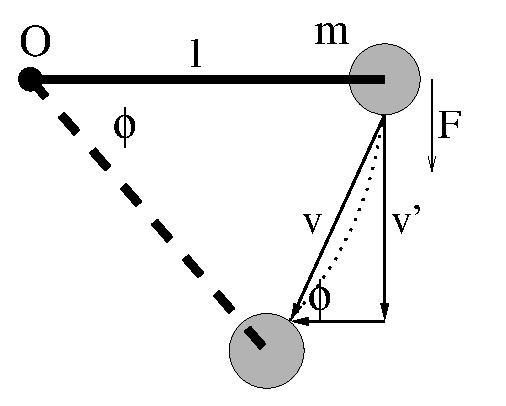
\includegraphics[width=0.7\textwidth]{bilder/hebel02}
   \caption[Hebel]{Skizze zu einem Hebel der L"ange $l$, der um $O$
     gedreht wird und an dessen Ende die Masse $m$ sitzt. Zwischen den
     beiden Zust"anden bewegt er sich mit der Geschwindigkeit $v$ um
     den Winkel $\phi$.}
   \label{abb_hebel}
\end{figure}


Auch f"ur den Drehimpuls gilt der \textbf{Impulserhaltungssatz} (siehe
Wichtig \ref{def_impulserhaltungssatz}):
\begin{Wichtig}
   [\index{Drehimpulserhaltungssatz}Drehimpulserhaltungssatz] Der
   Gesamtdrehimpuls eines Systems ist konstant.
\end{Wichtig}
Er l"asst sich nur "andern, wenn ein \emph{externes} Drehmoment
angreift! Dann ist das System aber nicht mehr abgeschlossen!



\begin{Beispiel}
Ein sch"ones Beispiel (bzw. Experiment) daf"ur kann man durchf"uhren,
wenn man auf einem Drehstuhl sitzt und eine rotierendes Rad mit der
Drehachse waagerecht vor sich h"alt. Durch den Drehstuhl k"onnen wir nur
den Drehimpuls bzw. Drehmoment nach oben betrachten -- einfach weil
in die anderen drei Raumrichtungen nicht rotiert werden kann, weil
keine Rotationsachse daf"ur vorhanden ist.

Kippt man nun das Rad "`seitw"arts"', so drehen wir seinen
Drehimpulsvektor praktisch mit. Je senkrechter die Drehachse also
steht, desto gr"o"ser ist der Anteil parallel zur Drehachse des
Stuhles\footnote{Formal bei einem Winkel $\varphi$ zwschen
  Stuhldrehachse und Raddrehachse gilt: $\vec L_{\bot
    \text{Stuhldrehachse}} = \vec L_{\text{Rad}} \cdot \cos \varphi$}
-- also desto mehr Drehimpuls k"onnen wir beobachten.

Da der Drehimpuls im System erhalten bleiben muss, dreht sich der Stuhl
in die Gegenrichtung: Er bringt einen eigenen Drehimpuls auf, sodass
die Summe der Drehimpulse verschwindet.   
\end{Beispiel}







\subsection{Kreisbewegung II}
\label{kap_kreisbewegung-ii}

Da
 $$\vec v = \vec \omega \times \vec r$$
mit dem \textbf{Drehvektor}
$\vec \omega,\; \omega = \frac{\diff \varphi}{\diff t}$ gilt f"ur den Drehimpuls bei einem
Kreis mit $\omega =
const$ und da $\vec \omega \bot \vec r$:\footnote{Um dies zu
  verifizieren, bildet man das Allgemeine Vektorprodukt der drei
  Vektoren: $\vec r \times \vec \omega \times \vec r $ (Im Folgenden
  die erste Zeile exemplarisch mit $\vec \omega = (u, v, w)$ und $\vec r
  = (x, y, z)$). In dem Vektor, den man als Ergebnis
  erh"alt, findet man in jeder Zeile zwei Quadratische Summanden und
  zwei ohne Quadrate: $uy^2 + uz^2 - vxy - zwx = u(y^2 + z^2) + x(-vy
  -zw)$. Die ohne Quadrate sind negativ
  %(bsp. 1. Komponente: $\omega_1(-\omega_2 r_2 - \omega_3r_3)$ 
  da nun $\vec \omega \bot \vec r$ ergibt sich daf"ur auch
  $ux + vy + wz = 0$ und damit $ux = -vy -wz$ und damit f"ur die erste
  Zeile $u(x^2 + y^2 + z^2) = \omega_1 \cdot r^2$. Die anderen Zeilen
  analog.

Einfacher geht es aber mit BAC-CAB:
$$
\vec r \times \vec \omega \times \vec r = \vec \omega (r^2) - \vec
r(\vec r\cdot\vec \omega) = \vec\omega \cdot r^2
$$}
\begin{equation}
   \label{eqn_drehimpuls-in-kreis}
   \vec L = m \cdot ( \vec r \times (\vec \omega \times \vec r) ) = m
   \cdot r^2 \cdot \vec \omega
\end{equation}

Wir k"onnen hier sch"on sehen, wie sich eine "Anderung von $r$ und $\vec
\omega$ auf das Drehmoment auswirkt. Dazu leiten wir
\eqref{eqn_drehimpuls-in-kreis} nach der Zeit ab:
\begin{equation}
   \label{eqn_differenz-c9}
   \frac{\diff \vec L}{\diff t } = \vec M = m 2r \dot r \vec \omega + m r^2
   \dot{\vec \omega}
\end{equation}
Wenn wir nun annehmen, dass wir uns ein einem abgeschlossenen System
befinden, so k"onnen wir annehmen, dass $\vec M = \vec 0$, dass von
au"sen also kein Drehimpuls auf den drehenden K"orper wirkt. Dann ergibt
sich
\begin{equation}
   \label{eq:30}
   2mr\dot r \vec \omega = - m r^2 \dot{\vec{\omega}} \text{ oder }
2\dot r \omega = -  r \dot\omega \text{ oder }
2\, \frac{\dot r}{r} = - \frac{\dot\omega}{\omega}
\end{equation}

Wird $r$ kleiner, so is $\dot r$ negativ. Um Gl. \eqref{eq:30} zu
gen"ugen, muss folglich $\dot{\vec \omega}$ positiv werden. D.h. der
K"orper macht eine schnellere Kreisbewegung.

Dies ist eine formale Erkl"arung daf"ur, warum man, wenn
man auf dem Eis eine Piruette dreht und dabei einmal die Arme weit von
sich gestreckt hat ($r$ gro"s) und immer schneller wird, wenn man die
Arme an den K"orper zieht ($\dot r < 0$ \Ipl $\dot{\vec \omega} > 0$).










\subsection{Im Zentralfeld}
\label{kap_im-zentralfeld}

\begin{Def}
   [\index{Zentralfeld}Zentralfeld]
Die Kraft $\vec F$ auf einen K"orper h"angt nur von der Entfernung vom
Zentrum des Feldes ab und zeigt immer parallel zu diesem Abstand:
\begin{equation}
   \label{eqn_def_zentralfeld}
   \vec F = \frac{\vec r}{\|\vec r\|} \cdot \gamma \cdot f(\|\vec r\|)
\end{equation}
wobei $\gamma$ eine Konstante ist und $f$ eine Funktion.
\end{Def}
Beispiele f"ur solche Felder sind \emph{Schwerkraft} oder
\emph{Coulomb-Anziehung}.


\begin{Wichtig}
F"ur eine Bewegung, die nur aufgrund der Kraft $\vec F$ aus diesem
Zentralfeld stattfindet, wird stets gelten: $\vec L = const$.    
\end{Wichtig}

Ganz
einfach deshalb, weil
$$
\vec F = f(r) \cdot \vec r ~ \Rightarrow ~ \vec M  = \vec r \times \vec F =
\vec 0
$$
(weil $\vec F \| \vec r$ gilt) und $\vec M$ ist die \emph{"Anderung} von $\vec L$.



\begin{Beispiel}
Es folgen nun f"ur Bewegung in Zentralfeldern die
\textbf{\textsc{\index{Kepler'sche Gesetze}Kepler}'schen Gesetze}:
\begin{itemize}
\item Die Bahn eines Teilchens liegt in einer Ebene.\footnote{Weil
     sonst ein $\vec M \neq \vec 0$ n"otig w"are}

Dies entspricht (etwa) dem \textbf{1. \textsc{Kepler}'schen Gesetz}:
\begin{quote}
   Planeten bewegen sich auf Ellipsenbahnen um ihr
   Zentralgestirn. Dieses steht in einem der Brennpunkte.
\end{quote}
Wir verwenden hier die N"aherung, dass Ellipsen- und Kreisbahnen sich
nicht sehr unterscheiden...
\item Der \textbf{\textsc{Kepler}'sche Fl"achensatz} also das
   \textbf{2. \textsc{Kepler}'sche Gesetz} gilt: 
   \begin{quote}
      Der Fahrstrahl\footnote{Ortsvektor mit der Sonne als Ursprung}
      $\vec r(t)$
      eines Planeten "uberstreicht in der gleichen Zeit $\diff t$ stets
      die gleiche Fl"ache $\diff A$.
   \end{quote}
Dies gilt, weil\footnote{$g$ und $h$ sind Grundseite und H"ohe im Dreieck} 
\begin{eqnarray*}
   \label{eq:32}
L &=& r \cdot mv \cdot \sin \varphi \\
&=& m \cdot \frac{1}{\diff t} \cdot \underbrace{\diff r}_g \cdot \underbrace{r
\sin
  \varphi}_h\\
&=& m \cdot 2 \cdot \frac{\diff A}{\diff t} = const
\end{eqnarray*}

\item Das \textbf{3. \textsc{Kepler}'sche Gesetz} besagt:
   \begin{equation}
      \label{eq:31}
      \frac{b^3}{T^2} = const
   \end{equation}
   wobei $T$ die Umlaufzeit und $b$ die L"ange der gro"sen Halbachse
   (also etwa der Radius: $b \approx r$) ist:

Da $F = \frac{mv^2}{r} = m\omega^2 r$ und $\omega = \frac{2\pi}{T}$
gelten und au"serdem $F = \gamma \frac{Mm}{r^2}$ folgt:
$$
m \left ( \frac{4\pi^2}{T^2} \right ) r = \gamma \frac{Mm}{r^2}
$$
und damit
$$
\frac{r^3}{T^2} = \frac{\gamma M}{4 \pi^2} = const
$$
\end{itemize}
\end{Beispiel}









\subsection{Mehrere Massenteilchen}
\label{kap_mehrere-massenteilchen}

Wir betrachtet $N$ Massenpunkte mit der Masse $m_i$ ($i = 1,...,N$)
die sich mit Kr"aften nach \eqref{eqn_def_zentralfeld} anziehen. In diesem
System
m"ussen wir unterscheiden zwischen 
\begin{description}[\setlabelstyle{\bfseries\slshape}]
\item[Innere Kr"afte] die die Teilchen aufeinander aus"uben:
   \begin{equation}
      \label{eq:34}
      \vec F_{ij} = \frac{\vec r_i - \vec r_j}{\|\vec r_i - \vec r_j\|}
      \cdot  f(\|\vec r_i - \vec r_j\|) 
   \end{equation}
\item["Au"sere Kr"afte] die von au"sen auf die $m_i$ wirken:
   \begin{equation}
      \label{eq:35}
      \vec F = \vec F_i^{ext}
   \end{equation}
\end{description}
Nun wollen wir die einzelnen Drehmomente betrachten:
\begin{eqnarray*}
   \label{eq:37}
\nonumber
   \vec M_i &=& \frac{\diff \vec L_i}{\diff t} = \vec r_i \times \vec
   F_i \\
&=&  \vec r_i \times \left ( \sum_{j = 1}^N F_{ij} + \vec F_i^{ext}
   \right )
\end{eqnarray*}
und damit das totale Drehmoment:
\begin{eqnarray}
   \label{eq:38}
\nonumber
\vec M_{ges} &=& \sum_{i = 1}^N \vec M_i \\
\nonumber
&=& \sum_{i = 1}^N \vec r_i \times \left ( \sum_{j = 1}^N F_{ij} + \vec
F_i^{ext}
   \right )\\
&=& \underbrace{\sum_{i,j = 1}^N \vec r_i \times F_{ij}}_{\vec 0} + \sum_{i =
1}^N \vec r_i \times \vec F_i^{ext} = \vec M^\text{ext}
\end{eqnarray}
Dabei k"urzt sich die erste Summe vollst"andig weg, weil zu jeder Kraft
$\vec F_{ij}$ eine \emph{Reactio} $\vec F_{ji}$ existiert -- und diese
ist gem"a"s Gl. \eqref{eqn_actio-reactio} betragsm"a"sig gleich aber von
der Richtung entgegengesetzt.

Wir haben so also gezeigt:
\begin{Wichtig}
   Die Inneren Kr"afte haben keinen Anteil am Gesamtdrehmoment und
   damit keinen Einfluss auf den Gesamtdrehimpuls.
\end{Wichtig}
Der Drehimpuls l"asst sich also nur durch ein externes Drehmoment
ver"andern -- was dem Drehimpulserhaltungssatz
(Kap. \ref{kap_drehimpuls}) entspricht!





















%%%%%%%%%%%%%%%%%%%%%%%%%%%%%%%%%%%%%%%%%%%%%%%%%%%%%%%%%%%%

%%%%%%%%%%%%%%%%%%%%%%%%%%%%%%%%%%%%%%%%%%%%%%%%%%%%%%%%%%%

%%%%%%%%%%%%%%%%%%%%%%%%%%%%%%%%%%%%%%%%%%%%%%%%%%%%%%%%%%%%







 \chapter{Mechanik des starren K"orpers}
\label{kap_mechanik-des-starren-korpers-1}


Wir betrachten nun starre, ausgedehnte K"orper. Anders als bei
Massenpunkten sind die Abst"ande zwischen den einzelnen Teilchen nun
fest -- die betrachteten K"orper sind nicht deformierbar (deswegen
hei"sen sie \emph{starr}).

Als "`Ersatz"' f"ur einzelne Massenpunkte $m_i$ k"onnen wir hier
verwenden:
\begin{equation}
   \label{eq:33}
   \diff m (\vec r) = \varrho (\vec r) \cdot \diff V
\end{equation}
wobei $\varrho(\vec r)$ die \emph{Dichte} des Stoffes am Ort $\vec r$
ist.









\section{Statik}
\label{kap_statik}


Hier wollen wir die Bedingungen untersuchen, unter denen sich ein
K"orper \emph{nicht} bewegt:

Anschaulich ist sofort klar:
\begin{Wichtig}
   [1. Bedingung f"ur mechanisches Gleichgewicht]
Die Summe der angreifenden Kr"afte muss verschwinden.
\begin{equation}
   \label{eqn_statik_bed_kraft}
   \boxed{
\sum_i \vec F_i = \vec 0
}
\end{equation}
\end{Wichtig}

In Abb. \ref{abb_wippe} ist dagegen eine Wippe abgebildet. Auch wenn
$F_1 + F_2 + F_c = 0$, so wird die Wippe dennoch kippen  -- ebenfalls
anschaulich klar.

Wir wir im Vorangegangenen Kapitel gesehen haben, wird auf die Wippe
so n"amlich ein \emph{Drehmoment} ausge"ubt, wodurch sich ein
\emph{Drehimpuls} ergibt, welcher f"ur das Kippen verantwortlich
ist.\footnote{Das Drehmoment von $F_e$ verschwindet, weil hier $\ell =
  r=
  0$. Au"serdem d"urfen wir ohne Kreuzprodukt rechnen, weil $r \bot F$
  und wir praktisch an den Betr"agen interessiert sind, \emph{weil wir
    die Richtung des Drehmoments wissen}.}
\begin{equation}
   \label{eq:36}
   \ell_1 \cdot F_1 + \ell_2 \cdot F_2 \neq 0 ~ \Rightarrow ~ L \neq const
\end{equation}
Damit wir $M_{ges} = 0$ bekommen, m"ussen wir {ersatzweise} die Kr"afte $F_2'$ und
$F_e'$ angreifen lassen. Dann gilt n"amlich:
\begin{Wichtig}
   [2. Bedingung f"ur mechanisches Gleichgewicht]
Die Summe der angreifenden Drehmomente muss verschwinden.
\begin{equation}
   \label{eqn_statik_bed_drehmoment}
   \boxed{
\sum_i \vec M_i = \vec 0
}
\end{equation}
\end{Wichtig}

\begin{figure}
   \centering
   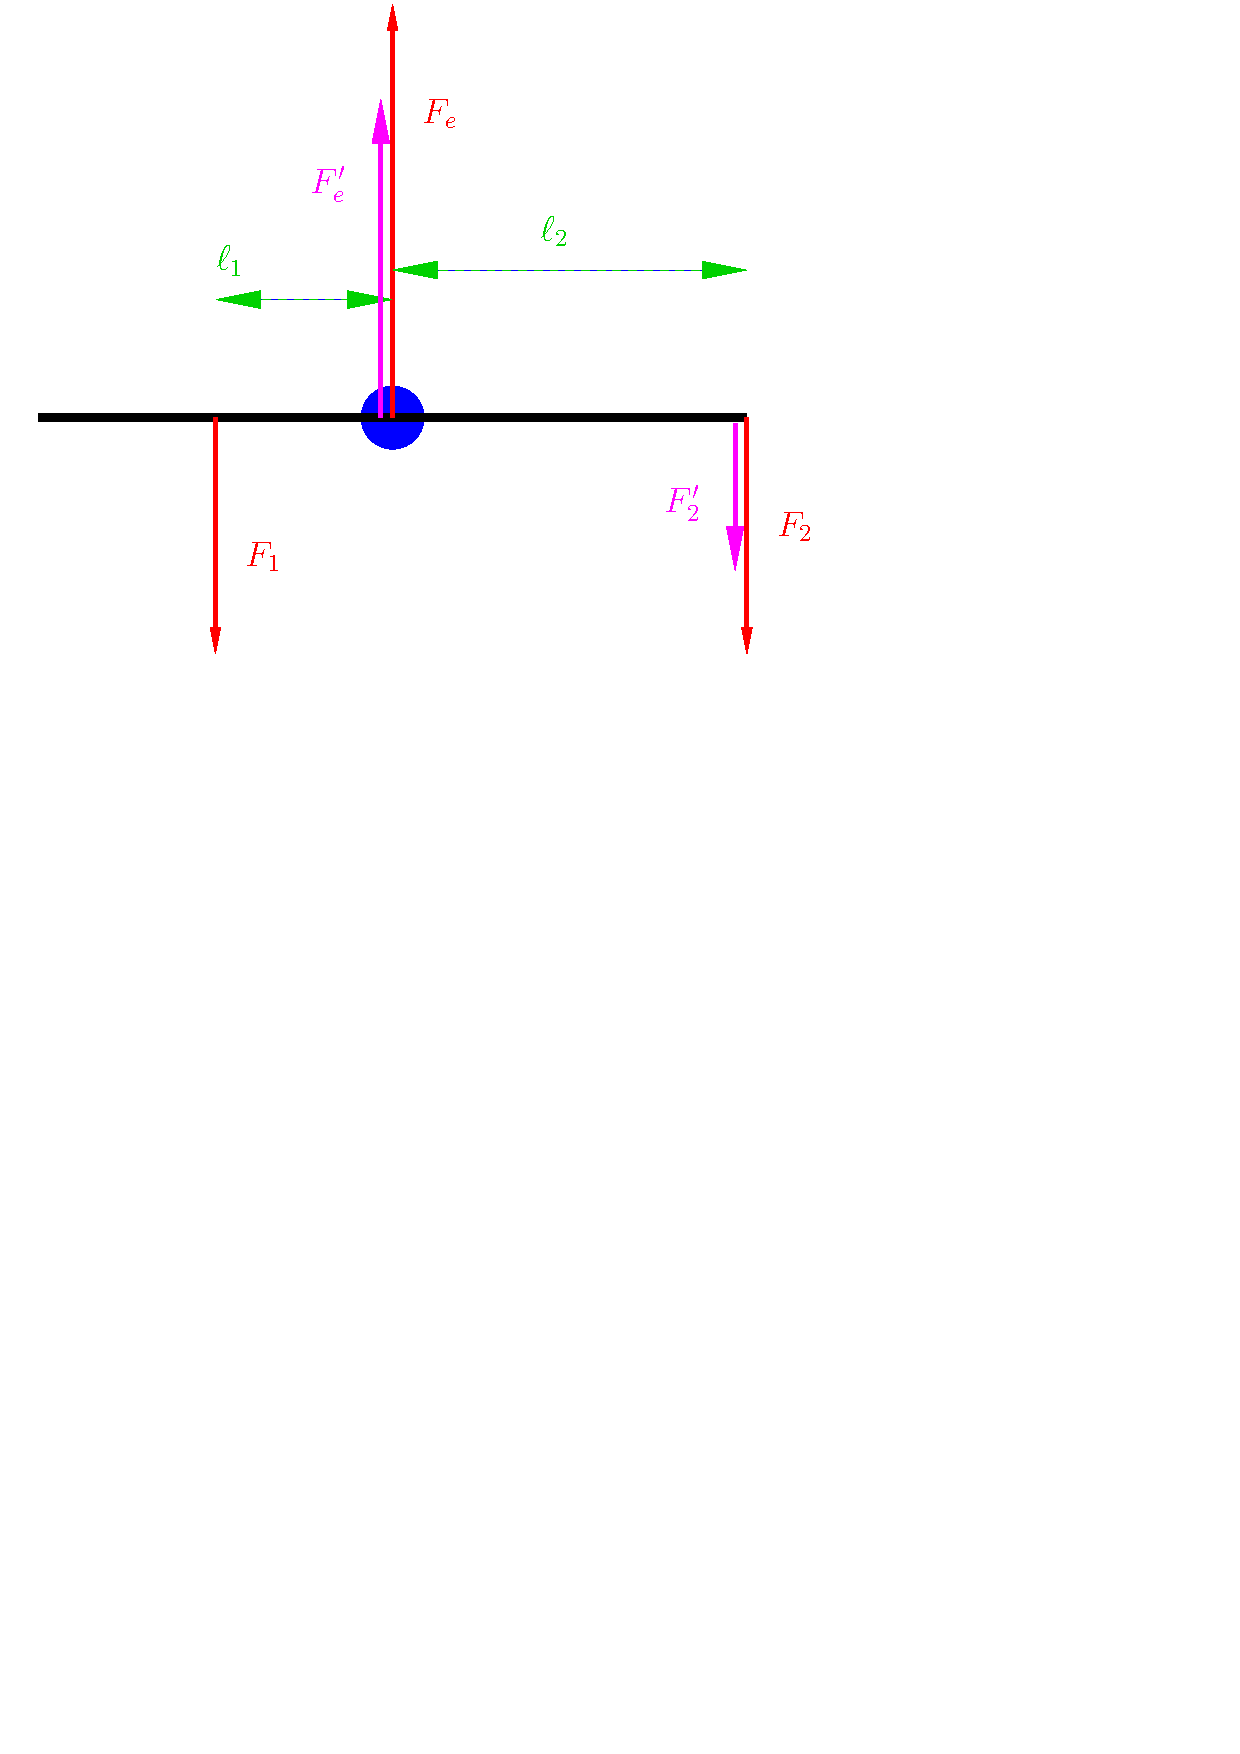
\includegraphics[width=0.7\textwidth]{bilder/wippe}
   \caption[Wippe im Gleichgewicht]{Wippe auf die Kr"afte wirken. Die
     Kr"afte $F_e'$ und $F_e$ sowie $F_2'$ und $F_2$ sollen \emph{am
       gleichen Punkt} angreifen.}
   \label{abb_wippe}
\end{figure}

\bigskip

Daraus folgen auch direkt die
\textbf{\index{Hebelgesetze}Hebelgesetze}: Damit der
Drehimpulserhaltungssatz gilt, muss
\begin{equation}
   \label{eqn_def_hebelgesetz}
   \boxed{
F_1 \cdot \ell_1 = F_2' \cdot \ell_2
}
\end{equation}
dabei werden die $\ell$ vom Hebelpunkt aus gemessen und die Kr"afte $F$
senkrecht zu $\ell$.

\bigskip

\subsubsection{verschiedene Arten von Gleichgewichten}
\begin{description}[\setlabelstyle{\bfseries\slshape}]
\item[Stabiles] Auf"angung "uber Schwerpunkt $S$\\Bei der Auslenkung wird
   $S$ angehoben und $E_{pot}$  steigt. Der K"orper wird sich also
   nicht von selbst auslenken, sondern in der Ruheposition -- auch bei
   kleinen St"orungen -- verharren.
\item[indifferentes] Die Aufh"angung liegt direkt auf dem Schwerpunkt
   $S$\\Bei Bewegung (Drehung) "andert sich weder $S$ noch
   $E_{pot}$. F"ur diese Aufh"angung sind (unendlich) viele verschiedene
   Orientierungen m"oglich.
\item[labil] die Aufh"angung liegt unter dem Schwerpunkt $S$\\Schon bei
   einer minimalen Auslenkung "`kippt"' das System und
   f"uhrt\footnote{bei Reibung -- hier schwingt es ged"ampft und kommt
     irgendwann zur Ruhe; ohne Reibung wird die Schwingung ewig gehen.} zu einer neuen Gleichgewichtslage.
\end{description}


\subsubsection{Standfestigkeit eines K"orpers}
\label{kap_standfestigkeit-korpers}

\begin{figure}
   \centering
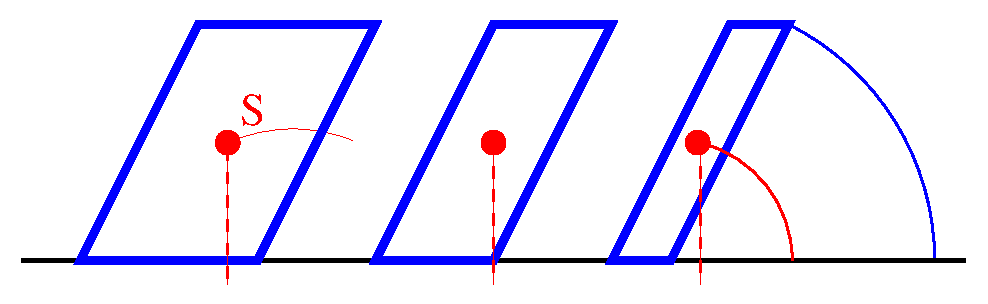
\includegraphics[width=0.7\textwidth]{bilder/schwerpunkt}
   \caption[Vergleich: Stabil, instabil]{Drei K"orper (vlnr): stabil,
     labil, wird gleich kippen}
   \label{abb_standfestigkeit}
\end{figure}

Falls die Projektion des Schwerpunkts $S$ auf die Grundfl"ache
au"serhalb der Standfl"ache selbst liegt, so wird der K"orper kippen.
Er dreht sich dann "uber seinen
\textbf{Drehpunkt}. (Vgl. Abb. \ref{abb_standfestigkeit}) Wenn der
Schwerpunkt wirklich "uber der Grundfl"ache ist, so m"usste der K"orper,
um zu kippen, seinen Schwerpunkt zuerst anheben und daf"ur br"auchte er
Energie. In Abb. \ref{abb_standfestigkeit} wird also nur der rechte
K"orper von selbst kippen -- hier kann der K"orperschwerpunkt bequem
(nur) nach unten fallen.




\section{Dynamik}
\label{kap_dynamik}

Wir unterscheiden zwischen \textbf{zwei Arten von Bewegung}:
\begin{description}[\setlabelstyle{\bfseries\slshape}]
\item[\index{Translation}Translation] Die Masse wird einfach
   verschoben. F"ur jeden einzelnen Massenpunkt gilt die gleiche
   Verschiebung: $\forall_i: \vec r_i \mapsto \vec{r_i}' = \vec r_i +
   \vec c(t)$. Dabei kann $\vec c$ nat"urlich von der Zeit abh"angen.

   Wir k"onnen uns dabei die gesamte Masse $M$ im Schwerpunkt des
   K"orpers konzentriert vorstellen.
\item[\index{Rotation}Rotation] Die einzelnen Massenpunkte werden
   abh"angig davon, wie weit sie vom Rotationszentrum entfernt sind,
   verschoben: $\forall_i: \vec r_i \mapsto \vec{r_i}' = \Mat{R} \cdot
   \vec r_i$. Dabei kann die Rotationsmatrix $\Mat{R} \in SO(3)$ von
   Zeit und Ort abh"angen.

Alternativ kann man eine Rotation auch mit $\vec \omega$ darstellen:
Der Drehvektor $\vec \omega$ laufe durch den Schwerpunkt $S$ des
K"orpers. Wir verwenden als Relativkoordinaten ein System mit $S$ als
Ursprung: $\vec r_{Si}$ beschreibt den Vektor zwischen $S$ und dem
$i$-ten Massenelement ($\vec r_{Si} = \vec r_i - \vec r_S$). Dann ist
die Rotationsgeschwindigkeit f"ur dieses Element gegeben durch
\begin{equation}
   \label{eqn_rotationsgeschwindigkeit}
   \vec v_r = \vec \omega \times \vec r_{Si}
\end{equation}
Dabei kann $\vec \omega$ nat"urlich wieder abh"angig von Ort und Zeit
sein.\footnote{Hier kann man sch"on die \emph{Rechte-Hand}-Regel
  anwenden: Rotiert ein K"orper, bildet der Daumen die Rotationsachse
  nach und die Finger der Faust zeigen in die Richtung der
  Drehung. W"ahlt man nun einen Vektor $\vec r$ so stellt man diesen
  mit dem Zeigefinger dar und erh"alt aus dem Mittelfinger die Richtung
  der Geschwindigkeit.}
\end{description}


\begin{Wichtig}
   Sobald eine Kraft an einem Punkt verschieden vom Schwerpunkt
   angreift, sorgt sie daf"ur, dass der K"orper rotiert.
\end{Wichtig}





\subsection{Drehimpuls eines starren K"orpers}
\label{kap_drehimpuls-starren-korpers}


Um den Drehimpuls eines K"orpers zu berechnen, m"ussen wir seine Form
und seine Massenverteilung einbeziehen. Wir zerlegen ihn im Allgemeinen
in unendlich viele kleine Massenelemente, deren Drehmomente wir
einzeln berechnen und schlie"slich aufaddieren:
\begin{equation}
   \label{eq:39}
   \vec L = \sum_i m_i \cdot (\vec r_i \times \vec v_i) = \sum_i \vec L_i
\end{equation}
Dabei gehen wir zum Grenzwert "uber und erhalten statt der Summe $\sum_i$
ein Integral $\int_V$.

Verwenden wir nun $\vec v_i = \vec \omega \times \vec r_i$, kommen wir
nach Gl. \eqref{eqn_drehimpuls-in-kreis} auf $\vec L_i = m_i \cdot
r_{\bot, i}^2 \cdot \vec \omega$. (Da der \emph{ganze} K"orper mit $\vec
\omega$ rotiert, ist das $\vec \omega$ an allen Stellen des K"orpers
gleich.)  Das $r_{\bot, i}$ bezeichnet den (senkrechten) Abstand von
$m_i$ zur Drehachse.  Verwenden wir nun anstelle der diskreten Massen
$m_i$ die Massenverteilung $\varrho(\vec r)$ (also $\diff m = \varrho
(\vec r) \diff V$), so erhalten wir aus Gl. \eqref{eq:39}:
\begin{equation}
   \label{eq:40}
   \vec L = \left ( \underbrace{\int_V \varrho(\vec r) \cdot  r_\bot^2 \diff V}_I
     \right ) \cdot \vec \omega
\end{equation}

\subsection{Tr"agheitsmoment}
\label{kap_tragheitsmoment}



\begin{Def}
   [\index{Tr"agheitsmoment}Tr"agheitsmoment]
\label{def_traegheitsmoment}
Das Tr"agheitsmoment 
\begin{equation}
   \label{eqn_def_traegheitsmoment}
   \boxed{
I = \int_V \varrho(\vec r) \cdot \vec r_\bot^2 \diff V
}
\end{equation}
"ubernimmt bei einer Drehbewegung die Rolle der Masse bei einer
geradlinigen Bewegung\footnote{Vgl. $\vec p = m \cdot \vec v$}. Hier
ist $\vec r_\bot$ senkrecht zu $\vec\omega$. Es gilt
\begin{equation}
   \label{eqn_drehimpuls-aus-traegheit}
   \vec L = I \cdot \vec \omega
\end{equation}
\end{Def}


Dabei muss $I$ jedoch kein Skalar sein -- $I$ ist vielmehr ein
\textbf{Tensor} $\Ten I$ (der zweiten Stufe\footnote{Geh"ort zu einer
  Linearen Abb. $R^n \to R^n$ -- hier $n = 3$.}). Das liegt daran, dass der
K"orper in verschiedene
Richtungen unterschiedlich einfach rotierbar ist.
Bspw. kann man einen Zylinder in einer Raumrichtung ohne
Energieaufwand rotieren (um ihre \emph{Rotations}achse) und in die
anderen nur schwer.

Der Tensor $\Ten I$ ist gegeben durch
\begin{equation}
   \label{eqn_traegheitstensor}
   \Ten I = I_{ij} = I_{ji} = \int_V \varrho(\vec r) \cdot (
   \delta_{ij}\vec r^2 - r^i \cdot r^j ) \diff V
\end{equation}
d.h. der Tensor ist \emph{symmetrisch}. Dabei stehen die Indizes $i$
und $j$ f"ur die $i$-te bzw. $j$-te Komponente des $\vec r$ im
Kartesischen Koordinaten (also ist bspw. $r^1 = x$). Entsprechend
hei"sen die einzelnen Elemente von $\Ten I$ auch $I_{xx}$, $ I_{xz}$, usw.

Um mit dem Tensor sinnvoll zu rechnen, kann man aus ihm das
\emph{Tr"agheitsmoment} $I_A$ bez"uglich einer Achse $A$ errechnen. Dazu
bildet man den Normalenvektor $\vec e_A$ parallel der Geraden mit
$\|\vec e_A\| = 1$ und multipliziert $\Ten I$ damit:
\begin{equation}
   \label{eq:44}
   I_A = {\vec e_A}^{T} \cdot  \Ten I \cdot \vec e_A
\end{equation}

\abs
Betrachten wir den Tensor als \emph{Matrix}, so wissen wir, dass man
jede symmetrische Matrix \emph{diagonalisieren} kann. D.h. wir k"onnen
eine \textbf{Hauptachsentransformation} durchf"uhren, bei der wir unser
Koordinatensystem so w"ahlen, dass unser "`neuer"' Tr"agheitstensor nur
noch auf der Diagonalen Eintr"age hat.

Unsere neu gew"ahlten Koordinaten haben ihren Ursprung im Schwerpunkt
und stehen senkrecht aufeinander. Wir bezeichnen sie als 
\begin{Def}
   [\index{Haupt(tr"agheits)achsen}Haupt(tr"agheits)achsen]
F"ur Rotationen um die Hauptachsen ($\vec \omega_a$, $\vec \omega_b$,
$\vec \omega_c$) ist das Tr"agheitsmoment ein Skalar
-- es ist also 
$$\vec L  ~ \| ~ \vec \omega$$
\end{Def}

Aus der Symmetrie\footnote{Die Symmetrie selbst folgt (auch) aus der Anzahl
  zur Verf"ugung stehender Freiheitsgrade: Eine Rotation im Raum ist
  durch  6 Freiheitsgrade festgelegt (Drei Winkel und drei
  Raumkoordinaten f"ur den Ursprung der Rotation). In unserer $(3 \times
  3)$-"'Matrix"' $\Ten I$ sind also nicht alle Eintr"age frei bestimmbar.} von
$\Ten I$ folgt, dass jeder K"orper \emph{drei} solcher
\emph{Hauptachsen} besitzt. Wie oben gezeigt, kann man jeder davon ein
Tr"agheitsmoment zuordnen. F"ur diese gilt logischerweise:
$$
I_a \leq I_b \leq I_c
$$
Diese bezeichnen wir auch als \textbf{ausgezeichnete} oder
\textbf{Haupt-Tr"agheitsmomente}. F"ur verschiedene Konstellationen
hei"sen die zugeh"origen K"orper\footnote{die "`$\neq$"' und "`$=$"'
  gelten oBdA}:
\begin{center}
\begin{tabular}{l l}
   $I_a = I_b = I_c$ & sph"arischer Kreisel \\
   $I_a \neq I_b = I_c$ & symmetrischer Kreisel \\
   $I_a \neq I_b \neq I_c$ & asymmetrischer Kreisel 
\end{tabular}
\end{center}


\subsubsection{Freie Achsen $(\bigstar)$}
\label{kap_freie-achsen}

Versetzt man einen K"orper in freie Rotation -- also h"alt keine
Rotationsachse k"unstlich fest -- so rotiert er nicht unbedingt einfach
weiter, sondern beginnt zu \emph{eiern}: 

$$
\vec L \not \parallel \vec \omega
$$

Bei folgenden (Sonder)F"allen eiern die K"orper \emph{nicht}, sonder
rotiert so, als w"are es eine feste Achse:
\begin{itemize}
\item Der K"orper rotiert nur um eine \textbf{Haupttr"agheitsachse}
\item Beim \textbf{sph"arischen} Kreisel
\item Beim \textbf{symmetrischen} Kreisel, der um eine Achse durch den
   Schwerpunkt und senkrecht zur Symmetrieachse rotiert. 
%Sicher: Demtroeder 1, S. 152.
\end{itemize}

\begin{Def}
   [\index{Freie Achsen}Freie Achsen]
sind die Achsen, um die ein K"orper ohne zu eiern rotieren kann, ohne dass man die Achsen festhalten muss.
\end{Def}

\begin{Wichtig}
   Experimentell ergibt sich, dass ein K"orper nur um die Achse seines
   miminalen $\vec I_a$ oder maximalen $\vec I_c$
   Haupttr"agheitsmoments \emph{stabil} rotieren kann.
\end{Wichtig}
Wenn er um die Achse $\vec \omega_b$ rotiert, so reicht schon die
kleineste St"orung aus, dass er zu torkeln beginnt.\footnote{Sch"ones
  Experiment: Ein Quader mit drei verschieden langen Seiten wird
  hochgeworfen und dabei um seine drei Symmetrieachsen rotiert. Bei
  einer der Achsen wirft man ihn hoch und f"angt ihn "`gespiegelt"'
  wieder -- er hat sich im Flug nicht nur um eine Achse gedreht.}




% Betrachten wir einen K"orper, der mit Drehgeschwindigkeit $\omega$ um
% eine bestimmte Drehachse $A$ rotiert ($\vec \omega \| A$), so k"onnen
% wir den Gesamtdrehimpuls  $\vec L$ berechnen, indem wir unseren
% Koordinatenursprung und eine Achse auf $A$ legen und jeden
% Ortsvektor $\vec r_i$ zerlegen in eine Komponente $\vec r_{i\|} \|
% A$ und eine Komponente $\vec r_{i\bot} \bot A$.

% F"ur den Drehimpuls sind nun nur die Vektoren $\vec r_{i\bot}$ wichtig,
% weil nur die \emph{Entfernung} des Massenteilchens von der Achse
% entscheidend f"ur den Drehimpuls ist.



\subsection{Kinetische Energie}
\label{kap_kinetische-energie}



M"ochten wir die \textbf{kinetische Energie} berechnen, die ein K"orper
bei seiner Rotation um eine Achse $A$ mit Rotationsvektor $\vec
\omega$ hat, so integrieren wir "uber die Kinetischen Energien seiner
Massenteilchen:
\begin{equation}
   \label{eq:41}
   E_{rot} = \sum_i \frac{1}{2}m_i v_i^2 = 
\sum_i \frac{1}{2} m_i (r_i \omega)^2 \to 
\int_V \frac{1}{2}\omega^2 m_ir_i^2 =
\frac{1}{2} \omega^2 \underbrace{\int_V r^2 \varrho \diff V}_I
\end{equation}

\begin{Wichtig}
   [Kinetische Energie einer Rotation]
Es gilt
\begin{equation}
   \label{eq:42}
   \boxed{
E_{rot} = \frac{1}{2} \cdot I \cdot \vec \omega^2
} = ~ ~  \frac{1}{2} \cdot \vec \omega^T \cdot \Ten I \cdot \vec \omega
\end{equation}
\end{Wichtig}
Die zweite Form wird verwendet, wenn das Tr"agheitsmoment als Tensor
$\Ten I$ vorliegt.

Vergleiche dazu auch 
$$
E_{kin} = \frac{1}{2} \cdot m \cdot \vec v^2
$$
d.h. wie in Def. \ref{def_traegheitsmoment} angesprochen "ubernimmt $I$
hier wieder die Rolle einer Masse.











\subsection{Drehimpuls verschiedener K"orper}
\label{kap_drehimpuls-verschiedener-korper}



\subsubsection{Rotationssymmetrischer K"orper}
\label{kap_rotationssymmetrischer-korper}

Zu jedem Massenelement $m_i$ geh"ort ein Element $m_i'$. Diese haben zu
$\vec L_{ges}$ die Beitr"age
\begin{eqnarray}
   \label{eq:43}
   \vec L_i &=& m_i \cdot (\vec r_i \times \vec v_i)\\
\nonumber
   \vec L_i' &=& m_i' \cdot (\vec r_i' \times \vec v_i')
\end{eqnarray}
Da der K"orper rotationssymmetrisch ist (Siehe dazu Abb. \ref{abb_rotsym}), ist
$m_i = m_i'$ und $\vec v_i
= - \vec v_i'$. Die Verbindung $\vec r_i - \vec r_i'$ verl"auft
\emph{senkrecht} zur zur Rotation $\vec \omega$. Wir verwenden
$\vec r_{i\bot} = \frac{\vec v_i
 - \vec v_i'}{2}$ (der senkrecht auf der Drehachse steht und zu $m_i$
bzuw. $m_i'$ zeigt), weil uns schlie"slich nur der Abstand von dem
Massenteilchen zur Rotationsachse interessiert.

Ein kleiner Beweis daf"ur\footnote{Aus "Ubersichtlichkeit wurden die
  Indizes gespart.}: Wir zerlegen den Vektor $\vec r$: $\vec r = \vec
r_\bot + \vec r_\|$, wobei $\vec r_\|$ parallel und $\vec r_\bot$
senkrecht zur Drehachse ist. Wegen $\dot{\vec r} = \vec \omega \times
\vec r$ ist 
$$
\vec L = m \vec r \times \vec v = m \vec r \times (\vec
\omega \times \vec r) = m (\vec r_\bot + \vec r_\|) \times (\vec
\omega \times (\vec r_\bot + \vec r_\|))
$$
Mit der Distributivit"at des Kreuzproduktes verschwinden "`hinten"'
Terme mit $\vec r_\|$, weil das Kreuzprodukt paralleler Vektoren
verschwindet:
$$
\vec L = m (\vec r_\bot + \vec r_\|) \times (\vec \omega \times \vec
r_\bot)
=
 m \vec r_\bot \times (\vec \omega \times \vec r_\bot)
+
 m  \vec r_\| \times (\vec \omega \times \vec r_\bot)
$$
Hierauf wendet man BAC-CAP an, und erh"alt:
\begin{equation}
   \label{eq:428}
\vec L = m\vec \omega (r_\bot^2) + m\vec r_\bot (\vec r_\bot \vec
\omega) + m\vec\omega(\vec r_\| \vec r_\bot) - m\vec r_\bot(\vec r_\| \vec \omega)   
\end{equation}
wobei die beiden mittleren Terme trivialerweise verschwinden, weil es
sich um Skalarprodukte orthogonaler Vektoren handelt. Man sieht:
\begin{Wichtig}
   Der Drehimpuls eines einzelnen rotierenden Massenpunktes ist nicht
   parallel zu $\vec \omega$ und ist zeitlich nicht konstant! Nur
   seine Komponente parallel zu $\vec \omega$ bleibt erhalten.
\end{Wichtig}
Weil wir aber f"ur jede Masse $m_i$ noch eine Masse $m_i'$ haben, die
gegen"uber rotiert, gilt f"ur diese $\vec r_\bot' = - \vec
r_\bot$. Addiert man die beiden Drehimpulse $\vec L_i$ und $\vec L_i'$
so f"allt auch der letzte Term aus \eqref{eq:428} weg und $\vec L$ ist
nur noch abh"angig von der Senkrechtkomponente $\vec r_\bot$ von $\vec
r$ und damit auch das Drehmoment.

 So fassen wir die
Beitr"age aus Gl. \eqref{eq:43} zusammen zu:
\begin{equation}
   \label{eq:45}
   \vec L_i^\sim = 
\vec L_i + \vec L_i' = 
m_i \cdot (\vec r_i \times v_i ) \mathbf{-}^\ast m_i' \cdot (\vec r_i'
\times \vec v_i) =
m_i \cdot ( \underbrace{(\vec r_i - \vec{r_i}')}_{2\vec r_{i\bot}} \times \vec
v_i)
\end{equation}
\footnote{Das "`$\mathbf -$"' bei $\ast$ kommt daher, dass $v_i =
  -v_i'$} Da nun $\vec\omega \times \vec r_{i\bot} = \vec v_i$ ist, gilt
mit \eqref{eqn_drehimpuls-in-kreis} weiter
\begin{equation}
   \label{eq:46}
      \vec L_i^\sim = 2 \cdot m_i \cdot r_{i\bot}^2 \cdot \vec \omega
\end{equation}
Wenn wir nun die einzelnen Drehimpulse f"ur alle Massenteilchen
aufaddieren, so d"urfen wir, wenn wir $\vec L_i^\sim $ verwenden
wollen, nur "uber die H"alfte der $i$'s summieren, weil in $\vec L_i^\sim
$ ja eigentlich \emph{zwei} Drehimpulse stecken. Alternativ k"onnen wir auch:
\begin{equation}
   \label{eq:47}
   \vec L_{ges} = \frac{1}{2} \sum_i \vec L_i^\sim  = \sum_i m_i \cdot
   r_{i\bot}^2 \cdot \vec \omega = I \cdot \vec \omega
\end{equation}
Beim "Ubergang zum Grenzwert (viele $i$-s und kleine $m$-s) erhalten wir:
\begin{equation}
   \label{eqn_I_rotsym}
\boxed{
   I_\text{rotsym} = \int_V r_\bot^2 \diff m = \int_V r_\bot^2 \varrho(\vec r)
\diff
   V
}
\end{equation}
Diese Integral "uber $V$ entspricht "ubrigens
$$
I = \int_{x_0}^{x_1} \int_{y_0}^{y_1} \int_{z_0}^{z_1} \varrho(x,y,z)
(r_\bot(x,y,z)) \diff x \diff y \diff z
$$


\begin{figure}
\centering
   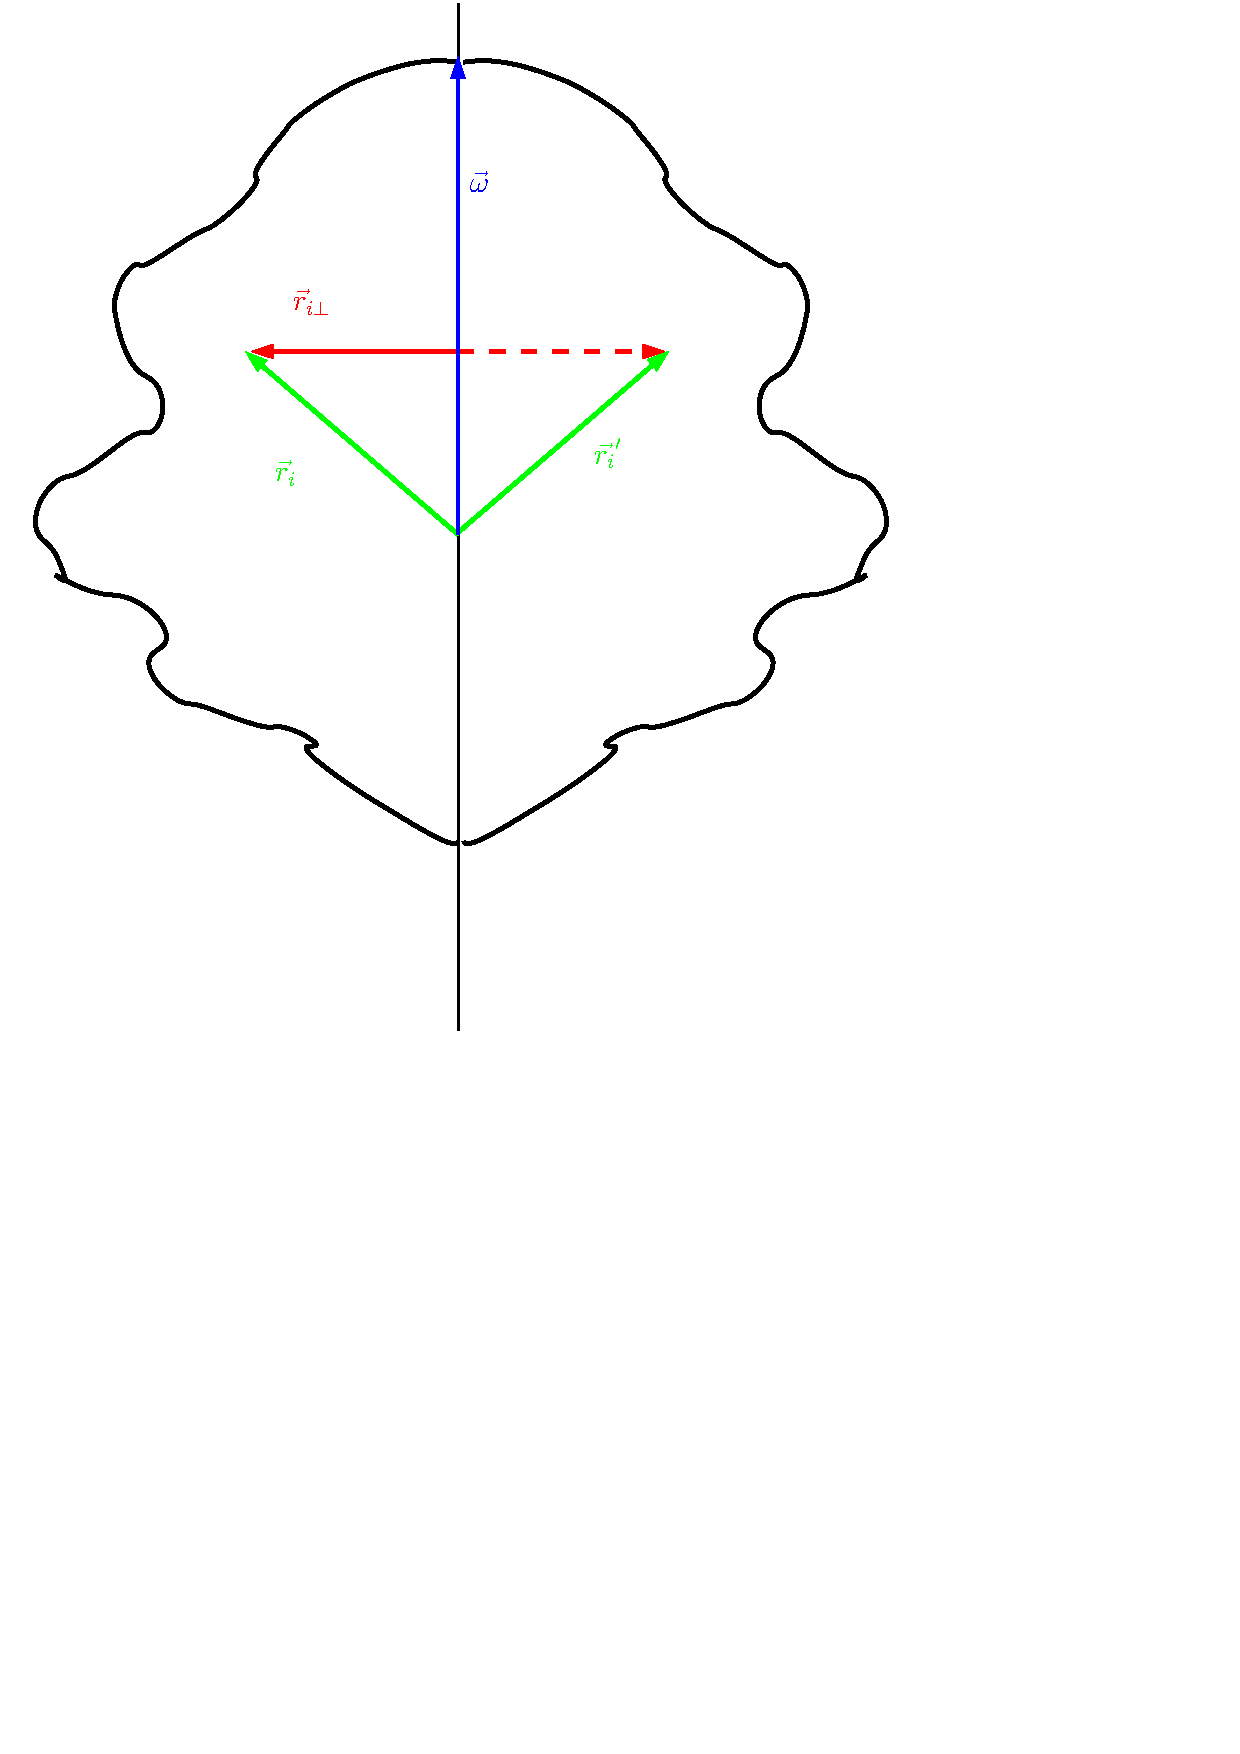
\includegraphics[width=0.5\textwidth]{bilder/rotsym}
   \caption[Drehung: Rotationssymmetrischer Körper]{Ein
     rotationssymmetrischer K"orper wird mit $\vec \omega$ gedreht.}
   \label{abb_rotsym}
\end{figure}




\paragraph{Beispiel: Homogene Kreisscheibe}
\label{kap_beispiel:-homogene-kreisscheibe}

Kreisscheibe der Dicke $D$ und mit dem Radius $R$. Wir arbeiten in
Zylinderkoordinaten: $\diff V = \diff z \cdot r \diff
\varphi \cdot \diff r$. Die (Massen)Dichte ist gleichverteilt: $\varrho =
\varrho_0 = \const$. 

$$
I = \varrho \int_0^R  \int_0^{2\pi} \int_0^D r^2 \diff z \cdot z \diff
\varphi \cdot \diff r = \frac{1}{2}  \underbrace{ \varrho \cdot
\underbrace{\underbrace{\pi
    R^2}_G \cdot D}_V}_M \cdot R^2 = \boxed{I_\text{Zyl} = \frac{1}{2}
M R^2 }
$$



 \paragraph{Beispiel: Hohlzylinder}
 \label{kap_beispiel:-hohlzylinder}


 \textbf{Hohlzylinder:}
Die Wandst"arke sei $d \ll R$. Wir ersetzen also das Integral
$\int_0^R\diff r$ gegen $\int_{R - d}^R\diff r$. Es ergibt
sich dann
$$
I =  2 \pi D \varrho \frac{1}{4} \left [ R^4 - (R-d)^4 \right ] = 
\frac{1}{2} \pi D \varrho [
\underline{4\, d\,{R}^{3}}-6\,{d}^{2}\,{R}^{2}+4\,{d}^{3}\,R-{d}^{4} ] \approx 2\pi
D \varrho R^3d
$$
Und f"ur die Masse ergibt sich
$$
M = \varrho \cdot [ \pi R^2 - \pi (R-d)^2 ] \cdot D = \varrho [
\underline{ 2\pi R d} - \pi d^2 ] \cdot D \approx 2 \varrho \pi R d D
$$
Und damit 
\begin{equation}
   \label{eq:48}
   \boxed{
I_\text{Hohlzyl} \approx M \cdot R^2
}
\end{equation}


Dabei haben wir beide Male eine h"aufig verwendete {N"aherung} gemacht
(bei den unterstrichenen Stellen): Da $d \ll R$, haben wir zuerst brav
mit $d$ und $R$ gerechnet, im Anschluss aber alle Terme, die $d$ in
einer h"oheren Potenz ($d^n$ mit $n \geq 2$) enthielten, einfach
weggelassen.

\begin{Wichtig}
   [\index{N"ahren}Technik: N"ahren]
M"ochte man einen sehr kleinen Wert $d$ ann"ahren, so l"asst man f"ur die
$n$-te N"aherung alle Summanden weg, die $d^m$ mit $m > n$ enthalten.

Bei Polynomen ist dies einfach, bei einer Funktion muss man diese
zuerst \textsc{Taylor}-entwickeln.
\end{Wichtig}

Alternativ h"atten wir die Rechnung auch mithilfe der
\emph{\index{Delta-Distribution}Delta-Distribution} machen k"onnen.
\begin{Beispiel}
   Dazu bestimmen wir die (homogene) "`Oberfl"achendichte"' $\sigma$
   mit $\sigma = \frac{M_0}{2\pi R L}$. Unser Integral vereinfacht
   sich dann zu ($r^2$ ist aus (\ref{eqn_I_rotsym}) und das weitere
   $r$ der Jacobian)
   \begin{equation*}
      I = \int_0^{2\pi} \int_0^L  \int_0^R \sigma r^3 \cdot \delta(R - r)
       \, \diff r \diff z
      \diff \varphi
   \end{equation*}
Das Argument der Delta-Distribution verschwindet bei $r = R$, damit
folgt f"ur das Integral
\begin{equation*}
   I = 2\pi \cdot L \cdot \sigma \, R^3 = 
2\pi \cdot L \cdot \frac{M_0}{2\pi R L} R^3 = 
M_0R^2
\end{equation*}
\end{Beispiel}




\subsubsection{Rotationssymmetrische K"orper, die nicht um K"orperachse Rotieren:
Satz von \textsc{Steiner}}
\label{kap_rotationssymmetrische-korper-nicht-um-korperachse}

Wenn die Rotationsachse \emph{parallel} zur K"orperachse verl"auft,
berechnen wir $I_S$ f"ur die K"orperachse (also die Achse, bez"uglich der
der K"orper symmetrisch ist). Dann gilt
\begin{Wichtig}
   [\index{Satz von \textsc{Steiner}}Satz von \textsc{Steiner}]
   \begin{equation}
      \label{eqn_satz_steiner}
      \boxed{ I = M \cdot a^2 + I_S }
   \end{equation}
mit Drehmoment $I_S$ auf der K"orperachse und Abstand $a$ zwischen
Rotations- und K"orperachse.
\end{Wichtig}













\subsection{Kreisbewegung III -- Der eiernde Kreisel}
\label{kap_kreisbewegung-iii-kreisel}


Wir betrachten einen starren, rotationssymmetrischen K"orper mit $\vec
L \| \vec \omega$ wobei keine "au"seren Drehmomente angreifen -- also
ist $\vec M = 0$ \Impl $\frac{\diff }{\diff t} \vec L = 0$ \Impl $\vec
L = \const$. Der Kreisel kreiselt also brav um seine Figurenachse...


Nun lassen wir eine Kraft $\vec F$ an der Kreiselachse angreifen --
und damit auch ein Drehmoment $\vec M = \vec r \times \vec F$ und
wollen damit den neuen Dreh\emph{impuls} des Systems bestimmen.

Wegen $\vec M = \dot{\vec L}$ k"onnen wir "uber die Zeit
aufintegrieren\footnote{Interessanterweise k"onnen wir an $\vec M =
  \dot{\vec L}$ auch sehen, dass $\vec M \| \diff \vec L$ sein muss.} und erhalten:
\begin{equation}
   \label{eq:49}
   \int_a^e \vec M \diff t = \int_a^e \dot{\vec L} \diff t = \vec L_e
   - \vec L_a = \Delta \vec L
\end{equation}
D.h. f"ur den resultierenden Drehimpuls $\vec L_e$ erhalten wir
\begin{equation}
   \label{eq:50}
   \vec L_e = \vec L_a + \int_a^e \vec M \diff t
\end{equation}
Da $\vec M \bot \vec L_a$ war, wird $\vec L_e$ \emph{nicht} parallel
zu $\vec L_a$ sein. Der Drehimpuls hat also seine Richtung
ge"andert. Wir zerlegen ihn in $\vec L_\|$ und $\vec L_\bot$ parallel
bzw. senkrecht zur Figurenachse.

"Uber den Zusammenhang $\vec L_i = I_i \cdot \vec \omega_i$ aus
\eqref{eq:44} wobei f"ur verschiedene Rotationsachsen in diesem Falle
$I_i \neq I_j$ -- also $I_\| \neq I_\bot$ -- gilt, ergibt sich so:
\begin{eqnarray}
\nonumber
   \vec L &=& \Ten I \cdot \vec \omega \\
\nonumber
   \vec L_\bot + \vec L_\| &=& I_\bot \cdot \vec \omega_\bot + I_\|
   \cdot \vec \omega_\| \\
   \vec L &\not \parallel & \vec \omega
   \label{eq:51}
\end{eqnarray}
Im Kap. \ref{kap_freie-achsen} haben wir gesehen, dass ein K"orper so
\emph{eiert}. Im speziellen, vorliegenden Fall, wird die Figurenachse
dabei auf einer Kegelfl"ache rotieren.



\begin{figure}[h]
   \centering
   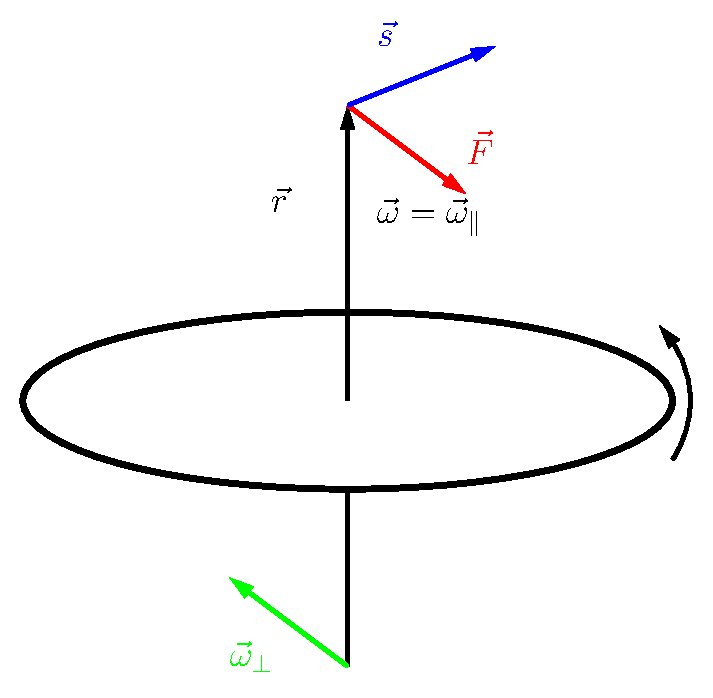
\includegraphics[width=0.7\textwidth]{bilder/kreiselsoerung}
   \caption[Gestörter Kreisel]{Der Kreisel wird mit der Kraft $\vec F$
     gest"ort.}
   \label{abb_kreiselstoerung}
\end{figure}

\bigskip


Wir betrachten jetzt einen \textbf{au"serhalb des Schwerpunkts
  aufgeh"angten Kreisel}: Der Kreisel kreiselt um seine K"orperachse und
deren Verl"angerung ist im Abstand $R$ (mit Vektor $\vec R$) vom
Schwerpunkt entfernt aufgeh"angt.

Es wirkt also die Schwerkraft $\vec F_g$ nach \emph{unten} und dadurch
wirkt auf den Kreis ein Drehmoment $\vec M = \vec R \times \vec F_g$
wodurch $\vec L = \vec L (t) \neq \const$ gilt. In
Abb. \ref{abb_kreisel_aeussere-aufhaengung} w"urde sich die Spitze von
$\vec R$ deswegen \emph{senkrecht} zur Papierebene bewegen -- wie in
Abb. \ref{abb_kreisel_vektoren} versuchsweise angedeutet ist.


Wegen $\vec M = \frac{\diff \vec L}{\diff t }$ gilt $\diff \vec L \|
\vec M$ und aus dem geometrischen Zusammenhang gilt $\|\diff \vec L \|=
\|\vec L \|\cdot \diff \phi$ so gilt auch
\begin{equation}
   \label{eq:52}
   \|\diff \vec L\| = \|\vec L\| \cdot \diff \phi = \|\vec M\| \cdot
   \diff t \text{ bzw. } \diff L = L \diff \phi = M \diff t
\end{equation}
Und der Vektor $\vec R$ w"urde sich mit einer Winkelgeschwindigkeit von 
\begin{equation}
   \label{eq:53}
   \omega_p = \frac{\diff \phi}{\diff t} = \frac{M}{L} = \frac{M}{I
     \cdot \omega} ~ \Rightarrow ~ \omega_p \sim \frac{1}{L} \sim \frac{1}{\omega}
\end{equation}
bewegen. Diese Bewegung nennt man
\textbf{\index{Pr"azession}Pr"azession}. Dabei ist $\omega$ die
Winkelgeschwindigkeit, mit der der Kreisel selbst um seine
K"orperachse rotiert und $\omega_p$ die \emph{Pr"azessionsfrequenz}.
 
\bigskip

Wenn der Kreisel nun anfangs nicht waagerecht aufgeh"angt war, sondern
der Winkel $\alpha$ zwischen $\vec L$ und $\vec F_g$ lag, so gilt
statt Gl. \eqref{eq:53}:
\begin{equation}
   \label{eq:54}
   \omega_p = \frac{\diff \phi}{\diff t} = \frac{M}{L \, \sin\alpha}
\end{equation}

\begin{figure}
   \centering \subfigure[\label{abb_kreisel_aeussere-aufhaengung}Kreisel mit Aufh"angung
   au"sen]{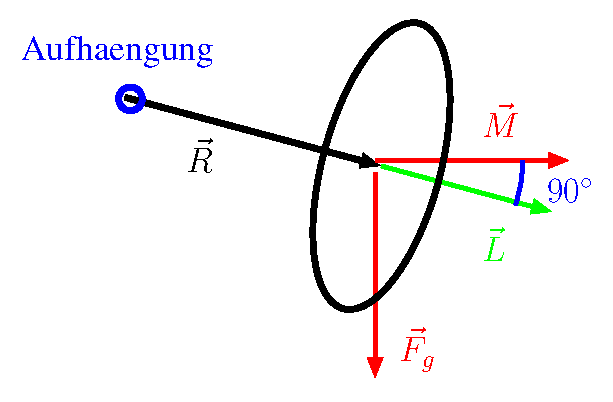
\includegraphics[width=0.5\textwidth]{bilder/praezessionA}}
   \subfigure[\label{abb_kreisel_vektoren}Die Vektoren]{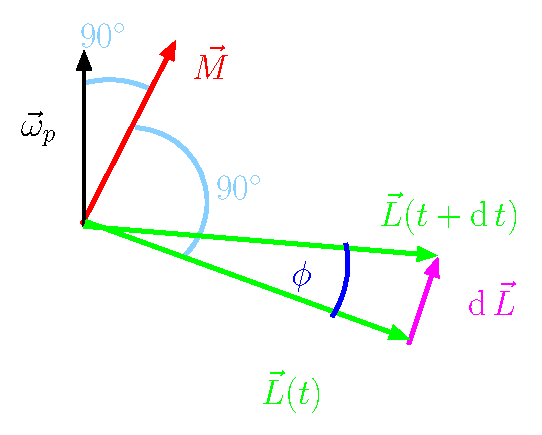
\includegraphics[width=0.4\textwidth]{bilder/praezessionB}}
   \caption{Abbildungen zur Pr"azession}
   \label{abb_preazession}
\end{figure}






\subsection{Ausblick: Quantisierung des Drehimpulses}
\label{kap_ausblick:-quantisierung-des-drehimpulses}

In der Quantenmechanik wird der Drehimpus eine \emph{gequantelte}
Gr"o"se sein -- also nur als (halb oder) ganzzahliges Vielfaches einer
fundamentalen Grundeineit auftreten. Diese Grundeinheit hei"st
\emph{\textsc{\index{Planck'sches Wirkungsquantum}Planck}'sches
  Wirkungsquantum} $\hbar$, also
$$
L = 2 \cdot n \cdot \hbar ~ ~  n \in \mathbb N
$$
wobei 
$$
\hbar = \frac{h}{2\pi} \approx 1,057 \cdot 10^{-34}
\frac{\operatorname{kg\,m^3}}{\operatorname{s}}
$$
Dabei gilt f"ur die Energie
$$
E = \nu \cdot h = \hbar \cdot \omega
$$

So tritt bspw. im hantelf"ormigen $\operatorname{N_2}$-Molek"ul der
Imupls auf als
$$
L = I \cdot \omega = 2mr^2 \cdot \omega = \hbar ~ \Rightarrow ~ \omega
= \frac{\hbar}{2mr^2}
$$
und mit eingesetzten Werten ($2r = 1,11 \operatorname{nm}$, $m = 2,3
\cdot 10^{-26}\operatorname{kg}$) bekommt man
$$
\omega \approx 7,5 \cdot 10^{11} \frac{1}{\operatorname{s}}
$$
und dies entspricht einer Frequenz im \emph{Infrarot}-Bereich.









\section{Vergleich Translation -- Rotation}
\label{kap_vergleich-translation-rotation}

\begin{center}

   \begin{tabular}{l c  l c}
      \toprule
      \textbf{Translation} &  \textit{Formel} & \textbf{Rotation} &
      \textit{Formel} \\
      \midrule
      L"ange & $l$, $s$ & Winkel & $\varphi$ \\
      Masse & $m$ & Tr"agheitsmoment & $\Ten I$ \\
      Geschwindigkeit & $\dot{\vec r} = \vec v$ &
      Winkelgeschwindigkeit & $\dot{\vec \varphi} = \vec \omega$ \\
      Impuls & $\vec p = m \cdot \vec v$ & Drehimpuls & $\vec L = \vec r
      \times \vec p = \Ten I \cdot \vec \omega$ \\
      Kraft & $\vec F = \frac{\diff \vec p}{\diff t }$ & Drehmoment & $\vec M =
      \frac{\diff \vec L}{\diff t}$ \\
      Kinetische Energie & $E_{kin} = \frac{1}{2}mv^2$ & Kinetische Energie
      & $E_{kin} = \frac{1}{2} I \vec \omega^2 = \frac{1}{2} \vec{\omega}^T \Ten I \vec \omega$ \\
      R"uckstellkraft & $\vec F = -D \cdot \vec r$ & R"uckstelldrehmoment &
      $\vec M = -D \cdot \vec \varphi$ \\
      \bottomrule
   \end{tabular}
\end{center}
























%%%%%%%%%%%%%%%%%%%%%%%%%%%%%%%%%%%%%%%%%%%%%%%%%%%%%%%%%

%%%%%%%%%%%%%%%%%%%%%%%%%%%%%%%%%%%%%%%%%%%%%%%%%%%%%%%%%

%%%%%%%%%%%%%%%%%%%%%%%%%%%%%%%%%%%%%%%%%%%%%%%%%%%%%%%%%



 \chapter{Mechanik deformierbarer K"orper}
\label{kap_mechanik-deformierbarer-korper}




Bisher hatten wir zwischen zwei Teilchen eines K"orpers starre
Verbindungen angenommen. Unsere Neuen Grundannahmen sind:

\paragraph{Bindungstypen zwischen Atomen}
\label{kap_bindungstypen-zwischen-atomen}

\begin{description}[\setlabelstyle{\bfseries\slshape}]
\item[\index{Ionische Bindung}Ionische] Bindungen: Durch die
   \emph{\textsc{Coulomb}-Kraft} werden geladene Teilchen angezogen
   und abgesto"sen. So h"alt bspw. $\operatorname{NaCl}$ zusammen.
\item[\index{kovalente Bindung}kovalente] Bindungen: Durch
   elektrostatische Wechselwirkungen werden nicht-ionische
   (Nichtmetall-)Atome und andere Teilchen zusammengehalten -- so bspw
   auch $\operatorname{H_2}$.
\item[\textsc{\index{Van-der-Waals-Kr"afte}Van-Der-Waals}]-Kr"afte:
   Durch Quantenmechanische Effekte halten neutrale Teilchen
   aneinander -- bspw. $\operatorname{Ar}$-Atome
\end{description}
Wir denken uns Festk"orper als Stoffe, die aus Atomen bestehen, die
\emph{feste} Pl"atze einnehmen. Die Atomen sind entweder geordnet und
bilden \textbf{\index{Kristalle}Kristalle} oder ungeordnet -- dann
hei"st der K"orper \textbf{\index{amorph}amorph} und wir bezeichnen
ihn als "`\textbf{\index{Glas}Glas}"'.


\paragraph{Erw"armung}
\label{kap_erwarmung}

Die Atome haben zwar eine Feste Position im Festk"orper, jedoch ist
dieser eigentlich nur eine \emph{Gleichgewichtslage}; sie k"onnen um
diesen herum \emph{Schwingungen} ausf"uhren.

Beim Erw"armen werden diese Schwingungen st"arker. "Uberhalb einer
kritischen Temperatur werden die Schwingungen so stark, dass sie die
Bindungskr"afte "uberwinden k"onnen und der Festk"orper so zerst"ort
wird. Das kennen wir als \textbf{\index{Schmelzen}Schmelzen}.


\paragraph{Festk"orper vs Fl"ussigkeiten}
\label{kap_festkorper-vs-flussigkeiten}

In Fl"ussigkeiten sind Atome gegeneinander verschiebbar d.h. sie haben
keinen Festen (Gleichgewichts-)Punkt und somit auch \emph{keine
  Formstabilit"at}. Dennoch ist die Dichte einer Fl"ussigkeit mit der
von Festk"orpern vergleichbar.

Beim Erw"armen schwingen auch hier die Atome schneller und wenn hier
die Kr"afte "uberwunden werden, die die Fl"ussigkeitsteilchen
zusammenhalten, so \textbf{\index{Verdampfen}verdampft} der Stoff.








\section{Deformierbare Festk"orper}
\label{kap_deformierbare-festkorper}


Wir n"ahren das Potential der Bindung zweier Atome mit dem Potential
einer Feder an. Dies ist eine N"ahrung, die nur in einem rechtkleinen
Bereich funktioniert. Das liegt daran, dass das Potential bei Atomen
in Kernn"ahe mit $V \sim \frac{1}{x^2}$ beschrieben wird und weiter
entfernt mit $V \sim -\frac{1}{x}$. Bei der Feder hingegen wird das
Potential nach $E_{spann} = \frac{1}{2}D \, \Delta x^2$ beschrieben
mit $V \sim (x-x_0)^2$. In Abb. \ref{abb_atompotential-federpotential}
ist Realit"at und N"ahrung\footnote{Also ein Potential $V =
  \frac{A}{x^2} - \frac{B}{x}$ mit weigehend beliebigen (positiven)
  $A$ und $B$ und eine Kurve mit $V_D = C\cdot (x-x_0)^2$ bei dem $C$
  und $x_0$ (m"oglichst) genau angepasst wurden. Dies gibt den Verlauf}
verglichen. \footnote{"Ubrigens ist dieses Atompotential ein
  Ausschnitt des Potentials in Abb. \ref{abb_kristallpotential}.}


Steigt die Temperatur im Feststoff an, so schwingen die Atome st"arker
um ihre Ruhelage. Im Diagramm hei"st das, dass sie eine h"ohere Energie
haben (also auf einem h"oheren Potential liegen, also im Schaubild
\emph{h"oher} sind) und damit weiter nach rechts (also weg vom Kern)
ausschwingen k"onnen, weil hier die Kurve f"ur das Potential im Atom ja
flacher wird. F"ur diesen Fall m"ussen wir eigentlich eine neue Parabel
anpassen, deren Mittelpunkt weiter nach rechts verschoben ist, um die
neue Situation besser zu modellieren


\begin{figure}
   \centering
   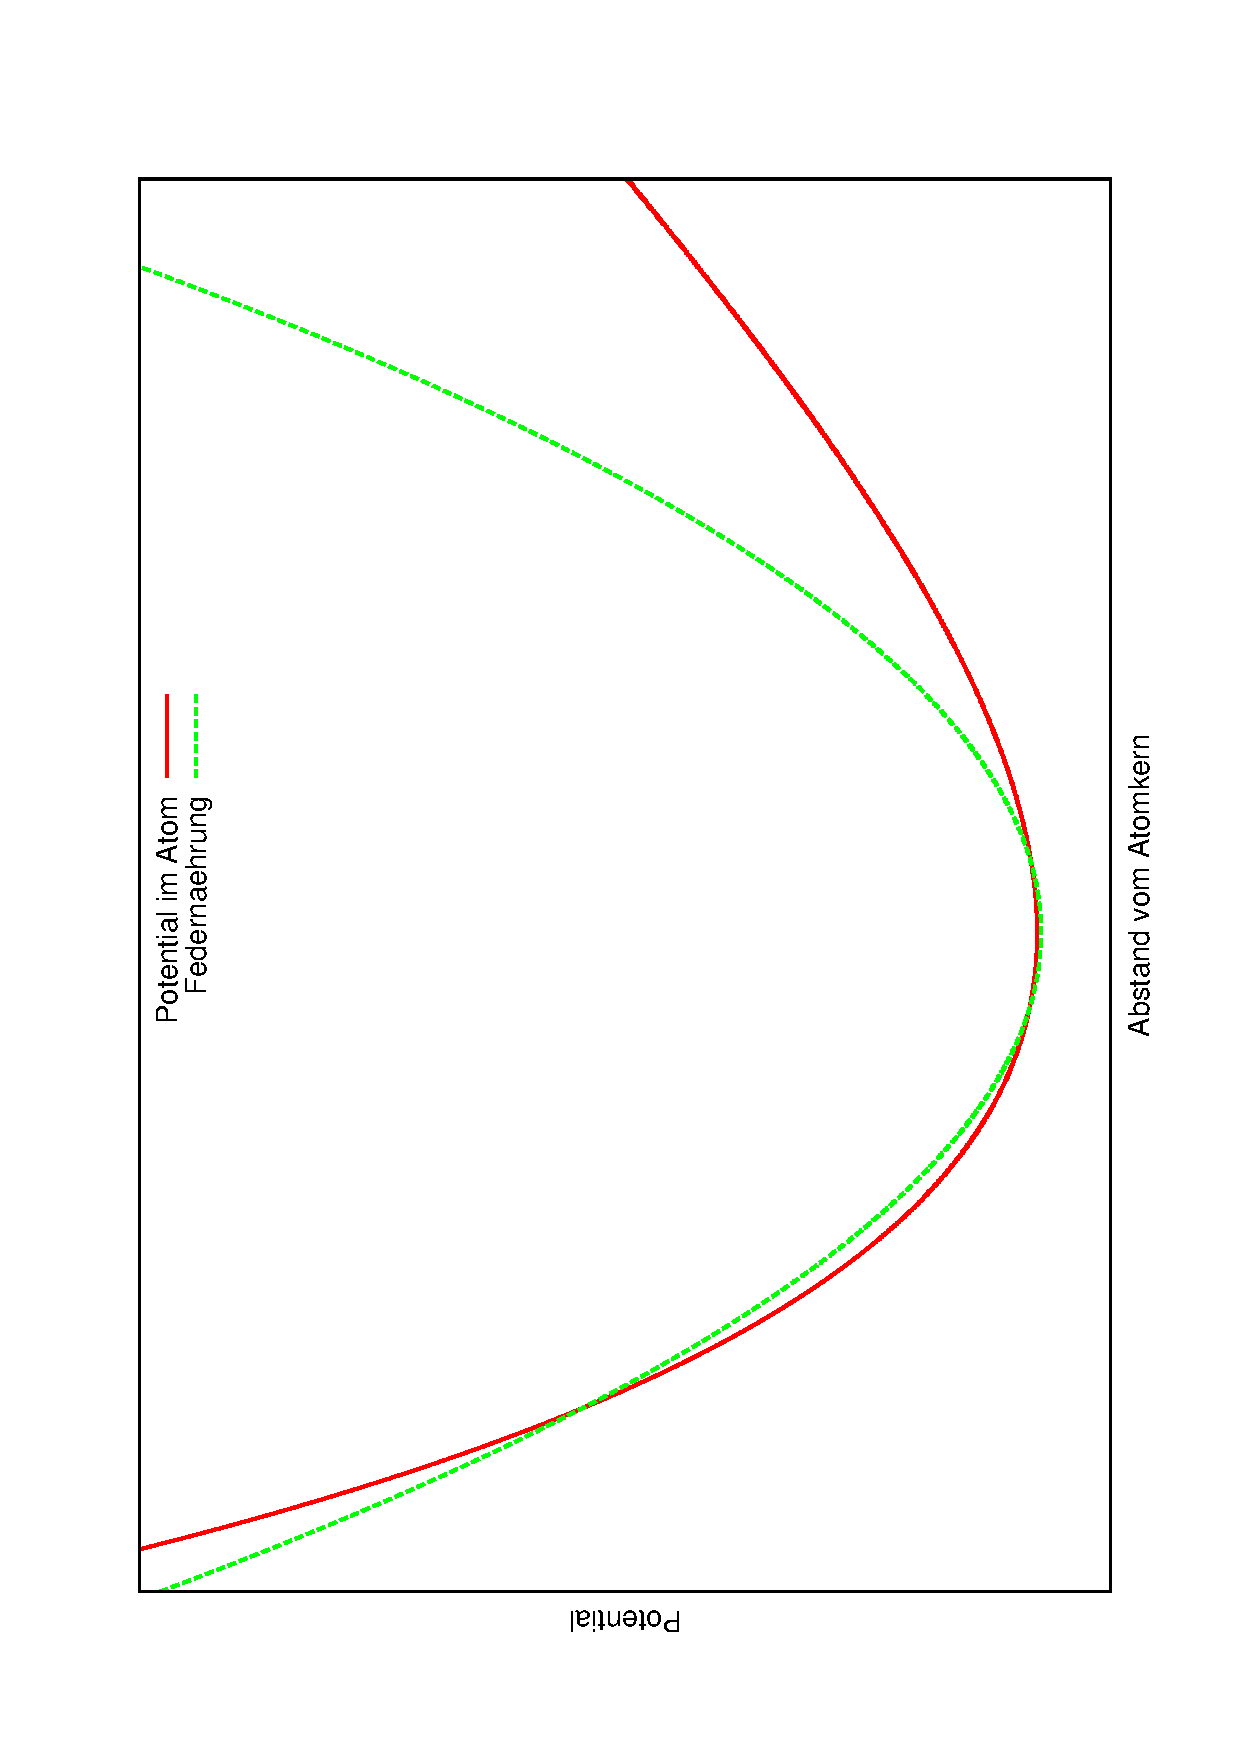
\includegraphics[width=0.7\textwidth,angle=-90]{bilder/atompot}
   \caption[Potentiale: Atomar, Feder]{Potential im Atom im Vergleich
     mit dem quadratischen Potential einer Feder}
   \label{abb_atompotential-federpotential}
\end{figure}

Wir verwenden diese Feder-N"aherung also im zul"assigen Bereich -- dort
wo sich in Abb. \ref{abb_atompotential-federpotential} die Kurven
weitestgehend "uberlappen -- und f"uhren das \textbf{Federmodell} ein.


\begin{Def}
   [\index{Federmodell}Federmodell]
Im Federmodell betrachten wir einen Festk"orper als punktf"ormige
Massen, die durch Federn verbunden sind.
\end{Def}



Mit diesem Modell k"onnen wir folgern, dass Festk"orper innerhalb
gewisser Grenzen \textbf{elastisch verformbar} sind:
\begin{Def}
   [\index{Elastisch}Elastisch verformbar]
Der K"orper ver"andert seine Form, wenn eine Kraft auf ihn ausge"ubt
wird, nimmt seine alte Form aber wieder an, wenn die angreifenden
Kr"afte verschwinden.
\end{Def}

Weil wir au"serdem die Parabel bei h"oheren Temperaturen nach rechts
verschieben m"ussen, bekommen die Ruhelagen der Atome einen gr"o"seren
Abstand zwischeneinander und somit \emph{expandiert} der K"orper
dann. Wir sprechen hier von einer \textbf{\index{thermische
    Expansion}thermische \index{Expansion, thermische}Expansion}.



\section{Kr"afte auf Festk"orper}
\label{kap_krafte-auf-festkorper}


\subsection{Dehnung}
\label{kap_dehnung}

Wir ziehen an dem Werkstoff der L"ange $L$ mit der Kraft $F$ (parallel
zu $L$) und dehnen ihn dadurch \textbf{absolut} um die Strecke $s$
bzw. Dehnung $\Delta L$ aus oder relativ um die
\textbf{\index{relative Dehnung}relative Dehnung} $\varepsilon =
\frac{\Delta L}{L}$. 


In Abb. \ref{abb_dehnung} ist eine Kurve einer typischen
Dehnung aufgetragen. Hier sieht man die verschiedenen staden
reversibler und irreversibler Verformung.

\begin{figure}
   \centering
   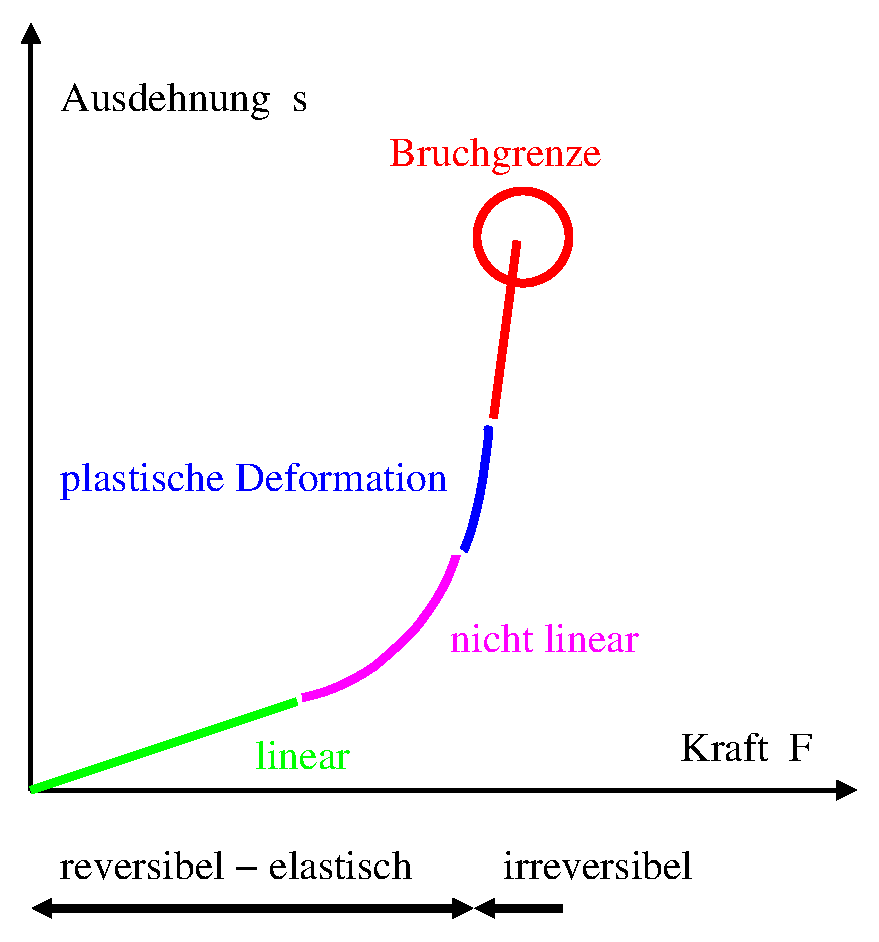
\includegraphics[width=0.7\textwidth]{bilder/dehnung}
   \caption{Dehnung eines Feststoffs im $s$-$F$-Diagramm}
   \label{abb_dehnung}
\end{figure}

Wir unterscheiden die angreifenden Kr"aften danach, wie sie angreifen;
entweder senkrecht zur K"orperoberfl"ache
oder waagerecht dazu. Wir wollen uns hier mit den Kr"aften
\emph{senkrecht} zur Oberfl"ache befassen:
\begin{Def}
   [\index{Zugspannung}(Zug-/\index{Druckspannung}\index{Spannung}Druck)Spannung
   \emph{"`\index{Stress"'}Stress"'} $\sigma$] Die Kraft ($\vec F_N$)
   zeigt senkrech ("`normal"') zur Oberfl"ache $A$ des K"orpers
\begin{equation}
   \label{eqn_Def_zugspannung}
   \sigma = \frac{\|\vec F_N\|}{A}
\end{equation}
\end{Def}
mit $[\sigma] = \frac{\operatorname{N}}{\operatorname{m^2}} = Pa =
10^{-5} \operatorname{bar}$


\bigskip

F"ur \textbf{kleine Amplituden} gilt f"ur die Verformung $\Delta L$ eines
K"orpers der L"ange $L$: 
$$
\Delta L \sim F \text{ , \;  } \Delta L \sim L \text{ und } \Delta L \sim \frac{1}{A}
$$
und so definieren wir:
\begin{Def}
   [\index{Elastizit"atsmodul}Elastizit"atsmodul $E$]
Eine \emph{Materialkonstante} f"ur die gilt
\begin{equation}
   \label{eqn_der_elastizitaetsmodul}
   E = \frac{\sigma}{\varepsilon} = \frac{F \cdot  L}{A \cdot \Delta
     L} ~ ~ \Leftrightarrow ~ \boxed{ \sigma = E \cdot \varepsilon }
\end{equation}
\end{Def}
Dieser Zusammenhang wird auch als \textbf{\textsc{Hook}'sches Gesetz}
bezeichnet. Vergleiche Dazu die \emph{Federh"arte} $D = \frac{F}{\Delta
L}$; 

\begin{quote}
   Je gr"o"ser $E$ ist, desto schwerer ist es -- also desto mehr Kraft
   $F$ muss man aufbringen -- um den K"orper um $\Delta L$ zu
   verformen.
\end{quote}


\emph{Eigentlich} m"ussten wir aber $E$ definieren als 
\begin{equation}
   \label{eq:55}
   E = \frac{\diff \sigma}{\diff \varepsilon}
\end{equation}
Nur weil wir im Bereich der linearen Expansion arbeiten
(s. Abb. \ref{abb_dehnung}) d"urfen wir die Definition oben verwenden.

\bigskip

\noindent
Wenn wir einen K"orper strecken, so werden wir beobachten, dass er
seinen Querschnitt verkleinert -- dies bezeichnet man als
\textbf{\index{Querkontraktion}Querkontraktion}. Man kann sie dadurch
erkl"aren, dass der K"orper bestrebt ist, sein Volumen gleich zu
halten.

Es gilt dabei -- wieder f"ur kleine Verformungen -- wenn wir eine
Querschnittsfl"ache mit $A = d^2$ annehmen (also $V = L\cdot d^2$):
Auch wenn der K"orper \emph{versuchen} mag, sein Volumen konstant zu
halten, so "andert es sich doch. Zieht man in L"angsrichtung an dem
K"orper, so verl"angert er diese Seite um $\Delta L$ ($\Delta L > 0$),
gleichzeitig werden sich die anderen Seiten $d$ verk"urzen ($\Delta d <
0$). Wir k"onnen f"ur die neuen L"angen also $L' = L + \Delta L$ und $d'
= d + \Delta L$ schreiben, und bekommen,
% $$
% V' = (d - \Delta d)^2 \cdot (L - \Delta L) = \underbrace{d^2 L}_V -
% 2d\Delta d \cdot L + (\Delta d)^2 \cdot L - d^2 \cdot \Delta L + 2 d
% \Delta d \cdot \Delta L - (\Delta d)^2 \cdot \Delta L
% $$
wenn wir in gewohnter Manier alle Therme streichen, die ein
quadratisches oder zwei verschiedene $\Delta$  enthalten:
$$
V' \approx V + 2d\Delta d L + d^2 \cdot \Delta L
$$
und weiter
$$
\Delta V \approx  d^2 \cdot \Delta L + 2d\Delta d L
$$
teilt man dies durch $V = d^2 \cdot L$ ergibt sich:
\begin{equation}
   \label{eq:56}
   \frac{\Delta V}{V} \approx \frac{\Delta L}{L} + 2 \frac{\Delta
     d}{d} = \varepsilon + 2 \varepsilon_q
\end{equation}
Dabei haben wir die \textbf{\index{relative Querkontraktion}relative
  \index{Querkontraktion}Querkontraktion $\varepsilon_q = \frac{\Delta
    d}{d}$} eingef"uhrt.  Das Verh"altnis zwischen (relativer)
Querkontraktion $\varepsilon_q$ und (relativer) Dehnung $\varepsilon$
bezeichnet man mit der \textbf{\index{Poissonzahl}Poissonzahl} oder
\textbf{\index{Querkontraktionszahl}Querkontraktionszahl}\footnote{Das
  "`$-$"' ist da, weil eine der beiden Kontraktionen $\varepsilon$
  oder $\varepsilon_q$ (praktisch) immer negativ ist, wenn die andere
  positiv ist -- dadurch erh"alt man ein positives $\mu$.}
\begin{equation}
   \label{eqn_def_poissonzahl}
   \mu = - \frac{\frac{\Delta d}{d}}{\frac{\Delta L}{L}} =
- \frac{\varepsilon_q}{\varepsilon} =
-   \frac{\Delta d \cdot L}{d \cdot \Delta L}
\end{equation}
und man erh"alt in Gl. \eqref{eq:56} durch Einsetzen:
\begin{equation}
   \label{eq:57}
   \boxed{\frac{\Delta V}{V} \approx \frac{\sigma}{E} ( 1 - 2\cdot \mu) }= (1
   - 2\mu) \cdot \varepsilon
\end{equation}


Im Allgemeinen ist 
$$
\Delta V < 0 ~ \Leftrightarrow ~ \mu > 0
$$
Es gibt aber auch bestimmte Stoffe, bei denen $\mu < 0$ ist -- der
Stoff wird also beim Ziehen l"anger \emph{und} breiter.




\subsection{Kompression}
\label{kap_kompression}


Wirkt eine \textbf{Kraft von allen Seiten} auf den K"orper, so hat er
keine andere M"oglichkeit, sich zu verformen und sein Volumen zu
verringern. 

Bei einem Druck $p$ -- f"ur den nach Definition $p = - \sigma$
gilt\footnote{Bei der Spannung $\sigma$ wirkt die Kraft nach au"sen,
  der Druck $p$ wirkt von au"sen auf den K"orper.} -- verk"urzt sich
eine Seite nach \eqref{eqn_der_elastizitaetsmodul} und mit $p =
\frac{F}{A}$ um $\Delta L = L \frac{\sigma}{E} = - L \frac{p}{E}$. Die
Seitenfl"achen mit L"ange $d$ w"urden sich eigentlich um $\Delta d = -
d \frac{p}{E}$ verk"urzen -- durch die Verk"urzung von $L$ muss $d$
sich aber noch zus"atzlich um $\Delta d = - \mu \frac{ \Delta L
  }{L} d = - \mu \cdot \frac{p}{E} \cdot d$ "andern. Diese zweite
"Anderung m"ussen wir auch noch doppelt gewichten, % weil sich eine
% Seite verl"angert, wenn eine andere sich verk"urzt -- in diesem
% 3-D-K"orper, auf den von allen Seiten Druck wirkt, "andern sich immer
% alle drei Seiten, also verk"urzen sich \emph{zwei} der anderen Seiten,
% wenn sich $d$ verl"angert.
%% neu folgt
weil die "Anderung einer der Kantenl"angen sich auf die "Anderung von
\emph{zwei} Kanten auswirkt -- und umgekehrt wirken auf die "Anderung
einer Kantenl"ange \emph{zwei} andere Kantenl"angen ein.

Diese Argumentation k"onnen wir f"ur jede der drei Seitenl"angen $\ell_i$ getrennt
durchf"uhren und kommen stets auf das selbe
Ergebnis:\footnote{Alternativ: Eine Seite verk"urzt sich um
  $\varepsilon = \frac{\sigma}{E}$ und so folgt f"ur eine beliebige
  andere $\varepsilon' = \varepsilon_q = - \mu \varepsilon = - \mu
  \frac{\sigma}{E}$. Eine Seite ver"andert sich also um $\varepsilon +
  2 \varepsilon'$ (die beiden gestrichenen Terme kommen von der
  Kontraktion der jeweils anderen Seiten) und so folgt
  $\varepsilon_\text{ges} = \frac{\sigma}{E} - 2 \mu \frac{\sigma}{E}$.}
\begin{equation}
   \label{eq:58}
   \Delta \ell_i = - \ell_i \cdot \frac{p}{E} ( 1 - 2 \mu)
\end{equation}
Wenn wir nun das Volumen mit Gl. \eqref{eq:56} berechnen wollen, so
vernachl"assigen wir wieder wie oben alle Terme mit mehreren $\Delta$s
und erhalten\footnote{Hier ist wichtig, dass die Poissonzahl $\mu$
  diesmal ein negatives Vorzeichen hat, weil sowohl $\varepsilon$ als
  auch $\varepsilon_q$ negativ sind!}
\begin{equation}
   \label{eq:59}
   \frac{\Delta V}{V} = \frac{\Delta L}{L} + 2 \frac{\Delta d}{d} =
   -3\frac{p}{E} (1 - 2 \mu) = - \frac{1}{K} \Delta p = - \kappa \cdot
   \Delta p
\end{equation}
Wobei wir definiert haben:
\begin{Def}
   [\index{Kompressionsmodul}Kompressionsmodul $K$, \index{Kompressibilit"at}Kompressibilit"at $\kappa$]
   \begin{equation}
      \label{eqn_def_kompressionsmodul}
      \kappa = \frac{1}{K} = - \frac{1}{\Delta p} \frac{\Delta V}{V} =
      \frac{3}{E}(1 - 2\mu) 
% \text{ bzw. } ~ \kappa \cdot \Delta p = -
%       \frac{\Delta V}{V}
\text{ bzw. } \boxed{\Delta p = - K\frac{\Delta V}{V}}
   \end{equation}
\end{Def}
Das Kompressionsmodul beschreibt also, welcher Druck n"otig ist, um
eine bestimmte relative Volumen"anderung hervorzurufen. Die
Kompressibilit"at zeigt den proportionalen Zusammenhang zwischen
Druck"anderung und relativer Volumen"anderung.




\subsection{Scherung}
\label{kap_scherung}

Analog zur Druckspannung senkrecht auf die Oberfl"ache eines K"orpers,
kann auch die Schubspannung $\vec F_T$  \emph{\textbf tangential} zur
Oberfl"ache wirken:

\begin{Def}
   [\index{Schubspannung}Schub/-\index{Scherspannung}Scherspannung $\tau$]
Die Kraft ($\vec F_T$) wirkt parallel der Oberfl"ache $A$ eines K"orpers
\begin{equation}
   \label{eqn_def_schubspannung}
   \tau = \frac{\|\vec F_T\|}{A}
\end{equation}
\end{Def}
mit der der Einheit $[\tau] = [\sigma] = \operatorname{Pa}$.

Nun untersuchen wir auch nicht mehr die "Anderung der Seitenl"ange,
sondern den sog. \textbf{\index{Scherungswinkel}Scherungswinkel}
$$
\alpha = \arctan \frac{\Delta L}{L}
$$

\begin{figure}
   \centering
   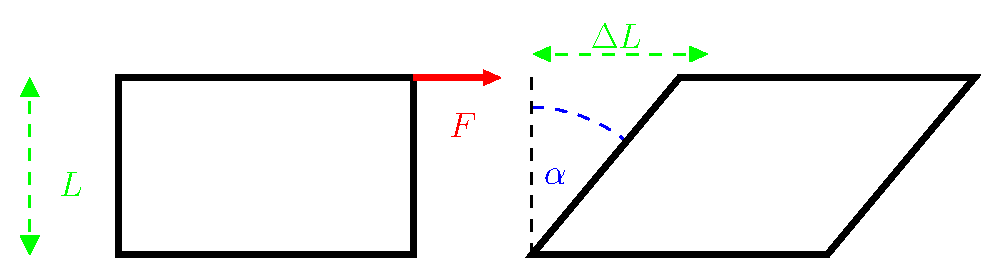
\includegraphics[width=0.7\textwidth]{bilder/scherung}
   \caption{Scherung eines K"orpers}
   \label{abb_scherung}
\end{figure}
Da f"ur kleine $x$ gilt\footnote{Der Taylor von Arctan um
  $0$: $$x-\frac{{x}^{3}}{3}+\frac{{x}^{5}}{5}-\frac{{x}^{7}}{7}+O(x^9)
  \text{ vgl Arcsinus: }
x+\frac{{x}^{3}}{6}+\frac{3\,{x}^{5}}{40}+\frac{5\,{x}^{7}}{112}+O(x^9)
$$}
$\arctan x \approx x$, setzten wir entsprechend
f"ur kleine Scherungen
\begin{equation}
   \label{eq:60}
   \alpha \approx \frac{\Delta L}{L}
\end{equation}
und definieren analog zum Elastizit"atsmodul:
\begin{Def}
   [\index{Schubmodul}Schubmodul $G$]
   \begin{equation}
      \label{eqn_def_schubmodul}
      G = \frac{\tau}{\alpha} ~ ~ \Leftrightarrow ~\boxed{\tau = G \cdot \alpha}
   \end{equation}
\end{Def}

Zwischen den Moduln $E$, $K$ und $G$ gilt im Allgemeinen:
\begin{equation}
   \label{eq:62}
   \boxed{
\frac{E}{2G} = 1 + \mu
} 
\text{ und }
\boxed{
\frac{E}{3K} = 1 - 2\mu
}
\end{equation}


Da bei einer Stauchung die Bindungs\emph{winkel} gleich bleiben, bei
einer Scherung dagegen die Bindungs\emph{l"angen}, und die jeweils
anderen Gr"o"sen sich ver"andern, brauchen wir die beiden Moduln:
\begin{Wichtig}
Ein K"orper reagiert im Allgemeinen verschieden darauf, ob er gedehnt oder
geschert wird...   
\end{Wichtig}




\section{Ruhende Fl"ussigkeiten}
\label{kap_ruhende-flussigkeiten}


\subsection{Oberfl"ache}
\label{kap_oberflache}


Die Teilchen einer Fl"ussigkeit k"onnen sich frei bewegen -- somit ist
ihre \emph{Position} logischwerweise nicht fest bestimmt. Bei der
\emph{Oberfl"ache} ist es jedoch anders: 
\begin{Wichtig}
Eine Fl"ussigkeitsoberfl"ache ist (nach einiger Zeit) immer senkrecht
  zur Summe aller einwirkenden Kr"afte.
\end{Wichtig}
W"are dies \emph{nicht} so, so w"urden die Teilchen an der Oberfl"ache
der Kraft folgen -- also in Richtung Kraft flie"sen. Dieses Verhalten
w"urde sich erst einstellen, wenn alle Fl"ussigkeitsteilchen auf einer
\emph{"Aquipotentialfl"ache} der angreifenden Kr"afte liegen, weil dann
keines mehr dazu neigt, seine Energie durch Bewegung im Potential zu
minimieren. 

\begin{Wichtig}
   In Fl"ussigkeiten verschwindet das Schermodul $G$.
\end{Wichtig}




\subsection{Stempeldruck}
\label{kap_oberflache-1}


Bei den \emph{Kr"aften auf eine Fl"ussigkeit} spricht man i.A. von
\textbf{Druck}.

\begin{Def}
   [\index{Stempeldruck}Stempeldruck]
Die Kraft $F$ wirkt senkrecht auf eine Fl"ussigkeitsoberfl"ache $A$,
dann gilt:
   \begin{equation}
      \label{eqn_def_druck}
      p = \frac{F}{A}
   \end{equation}
\end{Def}
mit der Einheit $[p] = \frac{\operatorname{N}}{\operatorname{m^2}} =
Pa$.

Den Druck kennen wir schon aus dem Zusammenhang mit der Kompression
eines Festk"orpers \eqref{eqn_def_kompressionsmodul}:
$$
\frac{\Delta V}{V} = -\kappa \cdot \Delta p
$$
Tabelle \ref{tab_kompressibilitaeten_fluessigkeit} zeigt, dass man in
guter N"aherung behaupten kann, dass:
\begin{Wichtig}
   Fl"ussigkeiten sind inkompressibel
\end{Wichtig}


\begin{table}
   \centering
   \begin{tabular}{l c}
      \toprule
\textbf{Stoff} & Kompressibilit"at $\kappa$ in
$\frac{1}{\operatorname{Pa}}$\\
\midrule
Wasser (bei $20^\circ\operatorname{C}$) & $46 \cdot 10^{-11}$\\
Eisen & $6.6 \cdot 10^{-11}$\\
Stickstoff & $1 \cdot 10^{-5}$\\
\bottomrule
   \end{tabular}
   \caption{Kompressibilit"aten von \emph{Fl"ussigkeiten}}
   \label{tab_kompressibilitaeten_fluessigkeit}
\end{table}




\subsection{Schweredruck}
\label{kap_schweredruck}



W"ahrend der Stempeldruck an jeder Stelle gleich wirkt, ist der
Schweredruck an verschiedenen Stellen verschieden. Er resultiert aus
der Gewichtskraft, die Teilchen weiter oben in der Fl"ussigkeit nach
unten aus"uben.

\begin{Def}
   [\index{Schweredruck}Schweredruck]
Die Fl"ussigkeitss"aule "uber einem Teilchen im Wasser erzeugt den Druck
\begin{equation}
   \label{eqn_schweredruck}
p = \int_0^h \frac{\diff F}{A} =
 \int_0^h \frac{g \cdot \diff m}{A} =
 \int_0^h \frac{g \cdot \varrho \cdot A \cdot \diff z}{A} =
\boxed{\varrho \cdot g \cdot h = p}
\end{equation}
\end{Def}
Und dabei gilt:
\begin{Wichtig}
   Der Schweredruck ist unabh"angig von der Fl"ache $A$.
\end{Wichtig}

Es kann auch vorkommen, dass die Dichte einer Fl"ussigkeit nicht
konstant ist. Bspw. wenn die Temperatur in verschiedenen Bereichen
verschieden ist, ist die Dichte im warmen Bereich \emph{kleiner}.
\begin{Wichtig}
   $$\varrho = \varrho(\vec r)$$
\end{Wichtig}
Siehe dazu Kap. \ref{kap_ruhende-gase}.


\subsection{Kommunizierende R"ohren}
\label{kap_kommunizierende-rohren}

% Wenn wir Rohre beliebig so befestigen, dass wenn man in eines Wasser
% sch"uttet, es \emph{nicht} aus dem System l"auft, sonder sich darin
% verteilt, so ist in allen R"ohren, die miteinander verbunden sind --
% und bei denen diese Verbindung auch unter Wasser steht -- der
% Wasserpegel gleich.

In ein beliebiges Rohrsystem wird Wasser gegeben. Wenn zwei R"ohren
miteinander verbunden sind, und das Wasser erreicht diese Verbindung,
so wird es durch diese Verbindung hindurchgedr"uckt: "uber dem einen
Rohr steht eine Wassers"aule, und mit diesem Druck werden die
Wasserteilchen in die n"achst Rohre gedr"uckt. Sie steigen aber dort nur
so hoch dass die Kr"afte auf die Teilchen in den S"aulen gerade
ausgeglichen sind. Nach Gl. \eqref{eqn_schweredruck} ist dies nur
m"oglich, wenn die Wasserpegel gleich hoch sind (eine konstante Dichte
angenommen). 

Dabei ist nur die \emph{H"ohe} entscheidend, weil in unserem Beispiel nur die
Schwerkraft eine \emph{Kraft} nach unten aus"ubt, die nach $F = m \cdot
a$ f"ur eine Bewegung ben"otigt wird.

\begin{Wichtig}
   [Prinzip der \index{Kommunizierende R"ohren}Kommunizierenden R"ohren] In miteinander verbundenen
   R"ohren ist der Wasserpegel unabh"angig von der Form gleich hoch.
\end{Wichtig}

Wir nehmen dabei stets die Schwerkraft als einzige Kraft an. Es kann
aber auch sein, dass noch andere Kr"afte auf die Fl"ussigkeit wirken.
\begin{Wichtig}
   Die Formel f"ur den Staudruck ist abh"angig von der \emph{Art} der
   Kr"afte, die auf die Fl"ussigkeit einwirken.
\end{Wichtig}



\subsection{Auftrieb: \textsc{Archimedis}ches Prinzip}
\label{kap_auftrieb:-archimedisches-prinzip}

Taucht man einen K"orper in eine Fl"ussigkeit und ist er
leichter\footnote{also weniger dicht} als diese, so erf"ahrt er hier einen
\emph{Auftrieb}, der darauf beruht, dass an seiner tiefer gelegenen
Unterseite ein h"oherer Druck $p_u$ als an seiner Oberseite $p_o$
herrscht. Daraus resultieren die Kr"afte $F_u$ und $F_o$, die in ihrer
Summe eine Kraft nach oben bilden.

Die Seitlichen Kr"afte auf den K"orper dagegen heben sich stets
gegenseitig weg, weil immer links und rechts die gleichen Kr"afte
wirken, weil die Punkte links und rechts per Definition auf der
gleichen H"ohe liegen.

Es gilt f"ur den Auftrieb $F_A = \|\vec F_A\|$ also:
\begin{equation}
   \label{eq:61}
   F_A = F_u - F_o =  \varrho \cdot g \cdot A \cdot \Delta h = \varrho
   \cdot g \cdot \Delta V = m \cdot g = F_{g, \text{Wasser}}
\end{equation}
\begin{Wichtig}
   [Archimedisches Prinzip]\index{Auftrieb}\index{Archimetisches Prinzip}
Der Auftrieb eines K"orpers entspricht der Schwerkraft der Verdr"angten
Menge Wassers.
$$
F_\text{ges} = (\varrho_\text{Wasser} - \varrho_\text{K"orper}) \cdot
g\cdot V
$$
\end{Wichtig}

Es sei wieder darauf hingewiesen, dass die Dichte konstant sein
muss -- wenn sie das nicht ist, gilt dieses Prinzip  nicht mehr exakt.

Wenn nun $F_\text{ges} > 0$, so schwimmt der K"orper, bei $F_\text{ges} = 0$
\emph{schwebt} er in der Fl"ussigkeit und bei $F_\text{ges} < 0$ geht er unter.

\bigskip

\begin{Beispiel}
Eine \textbf{Anwendung} dieses Prinzips ist die \textbf{Dichtemessung} von
Stoffen: Der K"orper wird an einen Feder-Newton-Meter geh"angt und die
auf ihn wirkenden Kr"afte in Wasser (oder einer anderen Fl"ussigkeit mit
definierter Dichte) und ohne Wasser verglichen. Die Differenz ist der
Auftrieb und damit ist die Dichte des Stoffes bestimmbar.   
\end{Beispiel}





\section{Grenzfl"achenspannung}
\label{kap_grenzflachenspannung}

Die hier behandelten Ph"anomene geh"oren eigentlich noch zu den ruhenden
Fl"ussigkeiten (Kap. \ref{kap_ruhende-flussigkeiten}).




\subsection{Kr"afte und Wechselwirkungen}
\label{kap_krafte-und-wechselwirkungen}



Wir betrachten verschiedene Wechselwirkungen:

\begin{Def}
   [\index{Koh"asion}Koh"asion]
Kraft zwischen
     Fl"ussigkeitsteilchen des selben Stoffs
\end{Def}
und 
\begin{Def}
   [\index{Adh"asion}Adh"asion]
Kraft zwischen Fl"ussigkeitsteilchen und anderem Stoff (Gef"a"swand)
\end{Def}
\begin{description}[\setlabelstyle{\bfseries\slshape}]
\item[Gef"a"swand--Fl"ussigkeit]   Wenn  das Wasser an der Wand "`hochklettert"', so spricht man
   von \textbf{Benetzung} (s. Abb. \ref{abb_benetzen}). F"ur diesen
    Effekt ist die \emph{Adh"asion} verantwortlich.

   \begin{figure}
      \centering
      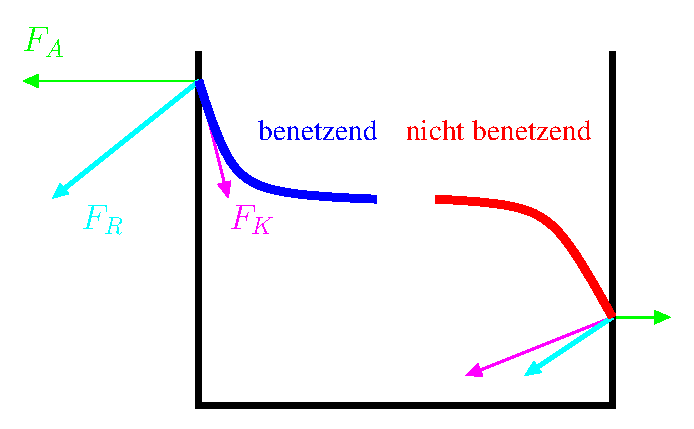
\includegraphics[width=0.4\textwidth]{bilder/benetzen}
      \caption{Wechselwirkungen bei Fl"ussigkeiten}
      \label{abb_benetzen}
   \end{figure}


\item[Fl"ussigkeit--Gas] \textbf{Im Inneren} der Fl"ussigkeit hat das Teilchen
   noch in alle Richtung benachbarte Teilchen und erf"ahrt so aus allen
   Richtungen die gleiche Kraft. In der Summe heben sich die Kr"afte
   weg und es herrscht insgesamt ein \emph{Kr"aftegleichgewicht}.

   \textbf{An der Grenzfl"ache} dagegen haben die Teilchen in Richtung
   der Grenzfl"ache keine Nachbarteilchen mehr. Hier wirken also
   Wechselwirkungen zwischen Teilchen und Nachbar in Richtung Inneres,
   die nicht durch entsprechende Gegenkr"afte \emph{weggehoben}
   werden. Es resultiert eine \emph{Kraft senkrecht zur Oberfl"ache
     nach innen}.

F"ur diese Kr"afte ist die \emph{Koh"asion} verantwortlich.
\end{description} 



Bewegt man ein Teilchen vom Inneren an den Rand, so ist eine Arbeit zu
verrichten: Im Inneren kann man das Teilchen noch ohne Kraft / Arbeit
bewegen; geht es jedoch auf den Rand zu, muss man es gegen eine Kraft
bewegen -- also Arbeit aufwenden. Um die Oberfl"ache $\Delta A$ zu
erzeugen, ben"otigen wir die Energie (die \emph{Arbeit}) $\Delta W$,
um die Teilchen gegen die nach innen wirkende Kraft nach Au"sen zu
bewegen, und es gilt $\Delta W \sim \Delta A$. Wir definieren als Ma"s
daf"ur:
\begin{Def}
   [\index{Oberfl"achenspannung}Oberfl"achenspannung $\sigma$]
   \begin{equation}
      \label{eqn_def_oberflaechenspannung}
      \sigma = \frac{\Delta W}{\Delta A} = \frac{F}{\ell}
   \end{equation}
mit $\ell$ als Randl"ange einer Fl"ussigkeitslamelle.

$\sigma$ hei"st auch "`\textbf{\emph{\index{Spezielle
      Grenzfl"achenenergie}Spezielle
    \index{Grenzfl"achenenergie}Grenzfl"achenenergie}}"'.
\end{Def}
mit der Einheit $[\sigma] =
\frac{\operatorname{J}}{\operatorname{m^2}} =
\frac{\operatorname{N}}{\operatorname{m}}$. Mit "`Lamelle"' ist hier
einfach ein (zweidimensional) gebogener B"ugel gemeint, der einen
zweidimensionalen Fl"ussigkeitsfilm auspannt. Dieser Film "ubt auf
seinen Rahmen die Kraft $F$ aus
Gl. \eqref{eqn_def_oberflaechenspannung} aus, wenn der B"ugel die
L"ange $\ell$ hat. Dabei ist wichtig, dass als Fl"ache $A$ nicht nur
eine Seite der Ebene, sondern beide gez"ahlt werden.

Anschaulich ist die Oberfl"achenspannung ein Ma"s daf"ur, wie
\emph{tragf"ahig} eine Fl"ussigkeit ist.

\begin{Wichtig}
   Die Oberfl"achenspannung ist gleich der
   \index{Oberfl"achenenergie}Oberfl"achen\emph{energie}.
\end{Wichtig}
Eine Fl"ussigkeitsoberfl"ache ist also so "ahnlich wie eine \textbf{elastische
Membran}. Der Unterschied ist aber, dass bei der elastischen Membran $F
\sim d$ ist (mit Auslenkung $d$), wobei bei Fl"ussigkeiten $F = \const$ gilt.



Die Oberfl"achenspannung ist sehr stark \emph{temperaturabh"angig}: Je
w"armer die Fl"ussigkeit ist, desto kleiner ist $\sigma$.



\subsection{Minimalfl"achen}
\label{kap_minimalflachen}


\begin{Wichtig}
   In der Natur bilden sich diejenigen Oberfl"achen mit der geringsten Oberfl"achenenergie.
\end{Wichtig}
\begin{Def}
   [\index{Minimalfl"ache}Minimalfl"ache]
Diese Fl"achen minimaler Oberfl"achenenergie nennen wir Minimalfl"achen.
\end{Def}


\subsubsection{Gekr"ummte Oberfl"achen}
\label{kap_gekrummte-oberflachen}

In einer \textbf{Seifenblase} herrsche der Druck $p_1$, au"serhalb der
Druck $p_0$. Hier konkurrieren nun zwei Kr"afte. Einerseits die Kraft
$F_1$, die aus den Druckverh"altnissen resultiert und nach au"sen
wirkt (weil $p_1 > p_0$):\footnote{Wir tun so, als best"unde die
  Seifenblase aus zwei Halbschalen; Die Kraft senkrecht zu einer
  gedachten Lamelle (einem Umfang) berechnet man mit der Effektiven
  Fl"ache $A = \pi r^2$. W"urde man die komplette Oberfl"ache der
  Halbschale verwenden, so w"urde man auch Kr"afte mit Anteil parallel
  zu $A$ mitnehmen.}
\begin{equation}
   \label{eq:88}
   F_1 = (p_1 - p_0) \cdot A = \Delta p \cdot \pi r^2
\end{equation}
und die Kraft $F_2$, die aus der Oberfl"achenspannung resultiert und
die Blase zusammenh"alt. Dabei haben wir eine Fl"ussigkeitslamelle mit
Rand $\ell = 2 \pi r$, die wir \emph{doppelt} werten, weil wir auch
einen \emph{doppelten} Phasen"ubergang haben: Diese Lamelle hat die
\emph{doppelte} Oberfl"ache, als eine gef"ullte Kugel h"atte.
\begin{equation}
   \label{eq:95}
   F_2 = \sigma \cdot 2\pi r \cdot 2
\end{equation}

Nun herrscht ein \emph{Kr"aftegleichgewicht} zwischen diesen Kr"aften,
also $F_1 = F_2$ und damit
\begin{equation}
   \label{eq:96}
   \Delta p \cdot \pi r^2 =  \sigma \cdot 4\pi r ~\Rightarrow ~ \Delta
   p = \frac{4 \cdot \sigma }{r}
\end{equation}

Wie bereits oben angedeutet ist bei einem  \textbf{Wassertropfen}
durch analoge "Uberlegungen die Formel
\begin{equation}
   \label{eq:97}
   \Delta p = \frac{2 \sigma}{r}
\end{equation}
korrekt, bei der wir nur eine Phasengrenze (au"sen) haben.

\bigskip

Im Allgemeinen gilt:
\begin{Wichtig}
   [\textsc{\index{Young-Laplace-Gleichung}Young-Laplace}-Gleichung] f"ur beliebig geformte Tropfen:
   \begin{equation}
      \label{eq:98}
      \boxed{
\Delta p = \sigma \left ( \frac{1}{r_1} + \frac{1}{r_2} \right ) }
   \end{equation}
$r_1$ und $r_2$ sind die \emph{Hauptkr"ummungsradien} der beiden Schmiegekreise an dem Punkt der Oberfl"ache, an dem die Druckdifferenz gesucht ist. Haupt- bedeutet hier den kleinst- und gr"o"stm"oglichen aller m"oglichen Kr"ummungsradien.
\end{Wichtig}


\subsubsection{Einfluss der Wand auf Minimalfl"ache}
\label{kap_einfluss-wand-auf-minimalflache}


Je nachdem, ob eine Fl"ussigkeit-Gef"a"s-Kombination benetzend ist oder
nicht, "andert sich entsprechend die Oberfl"ache. Wenn wir den Winkel
zwischen Fl"ussigkeitsoberfl"ache und Wand mit $\phi$ bezeichnen, so
erhalten wir f"ur \textbf{benetzende} Fl"ussigkeiten $\phi < 90^\circ$, f"ur
\textbf{vollst"andig benetzende} Fl"ussigkeiten $\phi \approx 0^\circ$
und f"ur \textbf{nicht benetzende} Fl"ussigkeiten $\phi > 90^\circ$.

Zu erkl"aren sind diese Formen durch die resultierenden Vektoren aus
Adh"askon un Koh"asion. In Abb.  \ref{abb_benetzen} sind die
entsprechenden Vektoren eingetragen.

Analog zu unseren "Uberlegungen aus \ref{kap_gekrummte-oberflachen}
m"ussen wir dann n"amlich noch die Kraft $F_R$ mit einbeziehen.



\subsection{Kapillarkr"afte}
\label{kap_kapillarkrafte}

Taucht man d"unne Rohre in eine Fl"ussigkeit so ist die Fl"ussigkeit in
dem Rohr nicht einfach nur senkrecht zur Schwerkraft sondern weist
eine Kr"ummung auf.  Zus"atzlich kann die Fl"ussigkeit sogar noch ein
St"uck in das Rohr (in die Kapillare) hineingezogen werden oder kann
innerhalb der Kapillare eine andere Wasserh"ohe als au"serhalb
erreichen.

Eine \textbf{benetzende} Fl"ussigkeit ist bestrebt, ihren Kontakt zur
Kapillare zu maximieren. Gegen die Kapillarkraft (aus
\eqref{eqn_def_oberflaechenspannung} mit $\ell = 2\pi r$ als Rand der
runden Kapillare)
\begin{equation}
   \label{eq:99}
F_\sigma = \sigma \cdot 2 \pi r   
\end{equation}
wirkt die Schwerkraft
\begin{equation}
   \label{eq:100}
   F_g = m \cdot g = \varrho V \cdot g = \varrho \cdot \pi r^2 h \cdot g
\end{equation}
 Im Gleichgewicht gilt $F_g = F_\sigma$ und damit ergibt sich f"ur die \textbf{Steigh"ohe}:
 \begin{equation}
    \label{eqn_kapillare}
\boxed{    h = \frac{2 \cdot \sigma}{\varrho \cdot r \cdot g} }
 \end{equation}

Betrachte man eine \textbf{nicht benetzende} Fl"ussigkeit, so gilt
Gl. \eqref{eqn_kapillare} ebenso -- nur dass $h$ jetzt nach
\emph{unten} geht; die Herleitung ist v"ollig analog.


\begin{figure}
   \centering
   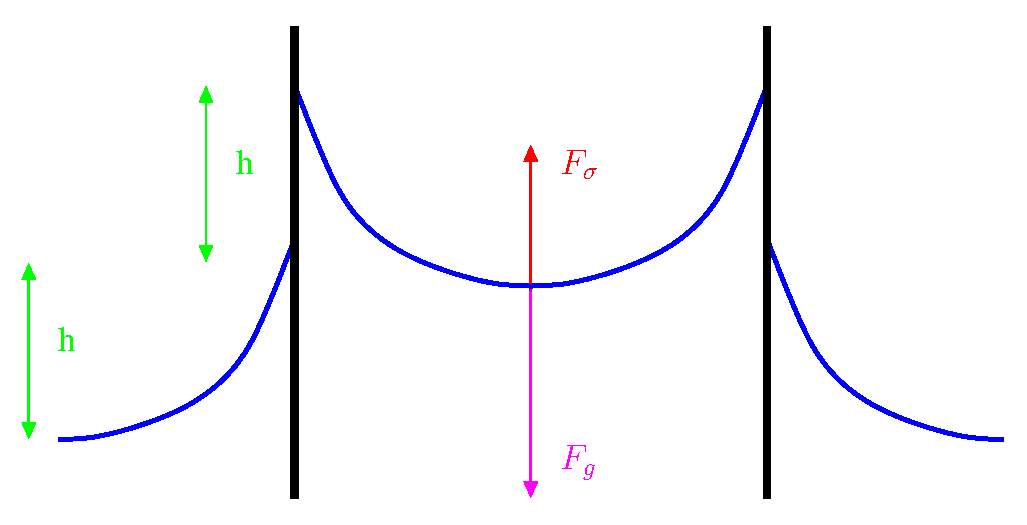
\includegraphics[width=0.6\textwidth]{bilder/kapillarA}
   \hfill
   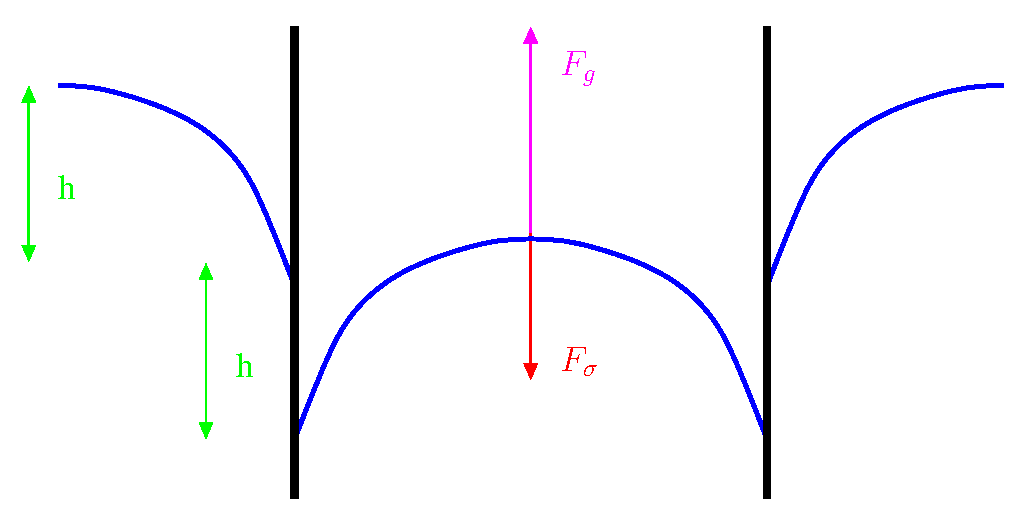
\includegraphics[width=0.3\textwidth]{bilder/kapillarB}
   \caption[Kapillarkräfte]{Kapillarkr"afte: Das rechte Bild ist
     einfach das Spiegelbild des linken, weil die Kapilarkr"afte f"ur
     benetzende und nicht benetzende Fl"ussigkeiten v"ollig analog
     sind.}
   \label{abb_kapillar}
\end{figure}







\section{Ruhende Gase}
\label{kap_ruhende-gase}

Wie Fl"ussigkeiten haben in Gasen die kleinen Teilchen keine feste
Position, daf"ur sind Gase aber komprimierbar.

Analog zur Fl"ussigkeit k"onnen wir hier den \textbf{Stempeldruck} definieren als
\begin{equation}
   \label{eq:63}
   p = \frac{\|\vec F^{(ext)}\|}{A}
\end{equation}
Wobei wir nicht mehr sagen k"onnen, dass eine Kraft senkrecht auf der
Gasoberfl"ache steht. Wir verwenden als Fl"ache $A$ also einfach die
Fl"ache des Stempels, die mit Gas in Kontakt kommt.

Wie wir in der Thermodynamik (Kap. \ref{kap_thermodynamik}) noch
ausf"urhlich sehen werden, gilt f"ur das Verhalten von \emph{idealen} Gasen
\begin{equation*}
   p \cdot V \sim T
\end{equation*}
Wobei \emph{ideale Gase} ein Modell f"ur Gase ist, welches die
Gasteilchen als kleine harte sto"sende Kugeln auffasst und bei kleinen
Dichten eine gute N"aherung darstellt.

\bigskip

Der \textbf{Schweredruck} bei Gasen ist ein wenig schwerer zu fassen:
Weil Gase kompressibel sind, ist 
\begin{Wichtig}
   $\varrho = \varrho(\vec r) = \varrho(h) \neq \const$.
\end{Wichtig}
Wir verwenden statt der eigentlichen Dichte $\varrho$ die
\emph{\index{Teilchendichte}Teilchendichte} $n = n(h) =
\frac{N}{V}$. Es gilt dann mit der idealen Gasgleichung
(s. Kap. \ref{kap_zustandsgroessen-und-gasgleichung}):
\begin{eqnarray}
   \label{eq:64}
\nonumber
   pV &=& NK_BT \\
\nonumber
   p &=& nK_BT
\end{eqnarray}
und f"ur $T = \const$ gilt:
\begin{equation}
   \label{eq:65}
\diff p = K_B T \cdot \diff n   
\end{equation}
Au"serdem gilt f"ur eine kleine Bewegung immernoch\footnote{F"ur
  imkompressible Stoffe gilt $p(h) = \varrho g \cdot h$
  (\ref{eqn_schweredruck}. F"ur einen kleinen Bereich $\diff h$ wollen
  wir nun annehmen, dass Luft auch eine konstante Dichte hat. Das
  "`$-$"' kommt daher, weil der Druck abnimmt ($\diff p < 0$), wenn
  man weiter hoch ($\diff h > 0$) geht.}
\begin{equation}
   \label{eq:66}
   \diff p  = -\varrho(h) \cdot g \cdot \diff h = -nm \cdot g \cdot
   \diff h
\end{equation}
wobei wir $\varrho = n \cdot m$ mit der Teilchenmasse $m$ gesetzt
haben: $n \cdot m = \frac{N \cdot m}{V} = \frac{M}{V} = \varrho$.

Aus Gl. \eqref{eq:65} und Gl. \eqref{eq:66} erhalten wir eine
Differentialgleichung:
\begin{equation}
   \label{eq:67}
    K_B T \cdot \diff n   =  -nm \cdot g \cdot
   \diff h
\end{equation}
Wir l"osen sie durch Trennung der Variablen 
$$
\frac{1}{n} \diff n = \frac{- m \cdot g}{K_B \cdot T} \diff h
$$
und anschlie"sendem Aufintegrieren\footnote{% Dabei ist $n(h =0)$ die
%   Anfgangsbedingung bzw. die Integrationskonstante. Diese wurde auf
%   der rechten Seite weggelassen, weil wir die Integrationskonstannte
%   der Rechten Seite einfach subtrahieren k"onnen und so in $n(h = 0)$
%   "`verstecken"' k"onnen.
  Dabei sind die Grenzen $0$ und $h$. Links wurde verwendet, dass $\ln
  a - \ln b = \ln \frac{a}{b}$ ist. Es ist $n(h = 0) = n_0$.}:
$$
\ln \frac n {n(h = 0)} = \int \frac{1}{n} \diff n = \int \frac{- m \cdot g}{K_B \cdot
  T} \diff h = -\frac{ m \cdot g }{K_B \cdot T}\cdot h
$$
Und um den $\ln$ aufzul"osen verwenden wir die $\exp$-Funktion
\begin{equation}
   \label{eq:68}
n(h) = n_0 \cdot \exp \left ( -\frac{m \cdot g }{K_B \cdot T}\cdot h \right )  
\end{equation}
Und "uber den Zusammenhang $p = n K_B T$ folgt weiter
\begin{equation}
   \label{eq:69}
\boxed{   p(h) = {p_0} \cdot  \exp \left ( -\frac{m \cdot g \cdot h}{K_B \cdot T} \right )  }
\end{equation}
wobei $p_0 = n_0 \cdot K_B T$. Dies ist die
\textbf{\index{Barometrische H"ohenformel}Barometrische H"ohenformel}.









\section{Str"omende Fl"ussigkeiten und Gase}
\label{kap_stromende-flussigkeiten-und-gase}


\begin{Wichtig}
   Wir betrachten \emph{langsam} str"omende Fl"ussigkeiten und Gase mit 
$$
\text{Str"omungsgeschwindigkeit} < \text{Schallgeschwindigkeit}
$$
\end{Wichtig}
Dann k"onnen wir bei Gasen eine konstante Dichte annehmen.

Bei diesen Bedingungen verhalten sich Fl"ussigkeiten und Gase wie
\emph{Fluide} (s. Def. \ref{def_fluid} auf S. \pageref{def_fluid}).

\bigskip
Wir unterscheiden bei Fl"ussigkeiten je nach Reibung drei Typen:
\begin{description}[\setlabelstyle{\bfseries\slshape}]
\item[Z"ahe] Fl"ussigkeiten\\Die Reibung \emph{innerhalb} der
   Fl"ussigkeit dominiert. (Die Str"omungen in diesen Fl"ussigkeiten
   hei"st \textbf{\index{laminar}laminar}.)
\item[Ideale] Fl"ussigkeiten\\Die Reibung ist im Vergleich zur
   kinetischen Energie unbedeutend
\item[Reale] Fl"ussigkeiten\\Die Str"omung ist so schnell, dass
   \emph{Wirbel} entstehen; wir sprechen von einer
   \textbf{\index{turbulent}turbulenten
     Str"omung}. Tr"agheitseffekte der Teilchen sind wichtig.
\end{description}




\subsection{Z"ahe Fl"ussigkeiten}
\label{kap_zahe-flussigkeiten}

Taucht man zwei Platten mit Abstand $d$ in eine Z"ahe Fl"ussigkeit und
will eine davon l"angs mit $v_0$ bewegen\footnote{also stehen die
  Plattenfl"achen \emph{parallel} zur Bewegung}, so braucht man daf"ur
eine Kraft $F_\|$. Diese resultiert daraus, dass die Teilchen in der
unmittelbaren Umgebung der bewegten Platte mitbewegt werden und
ihrerseits ihre "`Nachbarn"' mitbewegen usw.

Die Geschwindigkeit, mit der die einzelnen Wasserteilchen zwischen den
Platten bewegt werden m"ussen, nimmt linear mit dem Abstand zur Platte
ab -- bei der ruhenden Platte sollte er verschwunden sein; wir
sprechen von einem \textbf{\index{lineares
    Geschwindigkeitsprofil}linearen
  \index{Geschwindigkeitsprofil}Geschwindigkeitsprofil}
(s. Abb. \ref{abb_linaers-geschwindigkeisprofil})

Experimentell lassen sich die Zusammenh"ange
$$
F_\| \sim v_0 \text{ , } F_\| \sim A \text{ und } F_\| \sim \frac{1}{d}
$$
ermitteln. Wir definieren nun:
\begin{Def}
   [\index{Viskosit"at}Viskosit"at $\eta$]
Das Ma"s f"ur die \emph{Z"ahigkeit} eines Stoffes:
   \begin{equation}
      \label{eqn_def_viskositaet}
      \eta = \frac{F_\| \cdot d}{A \cdot v_0}
   \end{equation}
\end{Def}
mit der Einheit $[\eta] = \frac{\operatorname{Ns}}{\operatorname{m^2}}
= \operatorname{Pa}\cdot \operatorname{s}$

Da sich die Str"omungsgeschwindigkeit $v$ nicht unbedingt linear
bez"uglich des Abstands $d$ verhalten muss, ist im Allgemeinen diese
Formel richtig:
\begin{equation}
   \label{eq:74}
   \vec F = \eta \cdot A \cdot \frac{\diff \vec v}{\diff d}
\end{equation}
Dabei kann man $\frac{\diff \vec v}{\diff d}$ interpretieren als das
\textbf{Geschwindigkeitsgef"alle}. Also je gr"o"ser dieses Gef"alle ist,
desto gr"o"ser die Kraft...

\bigskip

In einem \textbf{Rohr} wirkt sich das so aus, dass die
Fl"ussigkeitsteilchen in der Rohrmitte am schnellsten Str"omen und die
Geschwindigkeit nach au"sen abnimmt. Dabei nimmt die Geschwindigkeit
quadratisch-proportional nach au"sen hin ab
(s. Abb. \ref{abb_quadratisches-geschwindigkeitsprofil}).

Dabei besteht Reibung nicht nur zwischen Teilchen und Wand, sondern auch
zwischen den Teilchen selbst - sonst w"urden die Teilchen sich ab einer
gewissen Entfernung zur Rohrwand mit der gleichen Geschwindigkeit
bewegen.


% Wir wollen dies n"aher betrachten: Nach Gl. \eqref{eq:74}
% gilt gilt bei infinitissimaler Betrachtung (die Teilchen str"omen in
% $y$-Richtung, das Geschwindigkeitsgef"alle, welches wir betrachten
% wolln, ist in $x$-Richtung) an der linken Seite:
% \begin{equation}
%    \label{eq:72}
%    \diff F_1 = - \eta \cdot \frac{\partial v}{\partial x}|_{\vec r_l}
%    \diff y \diff z
% \end{equation}
% Dies ist die Reibungskraft, die die Fl"ussigkeit erf"ahrt, wenn das
% Fl"ussigkeitsvolumen $\diff V = \diff x \diff y \diff z$ nach rechts
% str"omt. Wie wir aus Gl. \eqref{eq:74} gesehen haben, ist
% die hier herrschende Geschwindigkeitsdifferenz daf"ur entscheidend.

% An der rechten Seite kommen wir formal auf die gleiche Gleichung (mit
% $\vec r_r$ statt $\vec r_l$:
% \begin{equation}
%    \label{eq:73}
%      \diff F_2 =  \eta \cdot \frac{\partial v}{\partial x}|_{\vec r_r}
%    \diff y \diff z
% = \eta \left ( \frac{\partial v}{\partial x}|_{\vec r_l} +
%    \frac{\partial^2 v }{\partial x^2} \diff x \right ) \diff y \diff z
% \end{equation}
% Dabei verwenden wir in der Klammer das linke Gef"alle und addieren
% gewisserma"sen die \emph{Ver"anderung des Gef"alles} im Verlauf der
% $x$-Achse dazu -- daher die zweite Partielle Ableitung.

% Wenn wir nun die resultierenden Reibungskr"afte bestimmen wollen, summieren wir
% \eqref{eq:72} und \eqref{eq:73}:
% \begin{equation}
%    \label{eq:75}
%    \diff F = \diff F_1 + \diff F_2 = \eta \cdot \frac{\partial^2
%      v}{\partial x^2} \underbrace{\diff x \diff y \diff z}_{\diff V}
% \end{equation}




\bigskip

Nach Carl von \textsc{Linné}s \emph{"`Die Natur macht keine Spr"unge"'}
gilt f"ur uns
\begin{Wichtig}
   Geschwindigkeitsprofile sind kontinuierlich.
\end{Wichtig}

\begin{figure}
   \centering
   \subfigure[Linear bei zwei
   Platten]{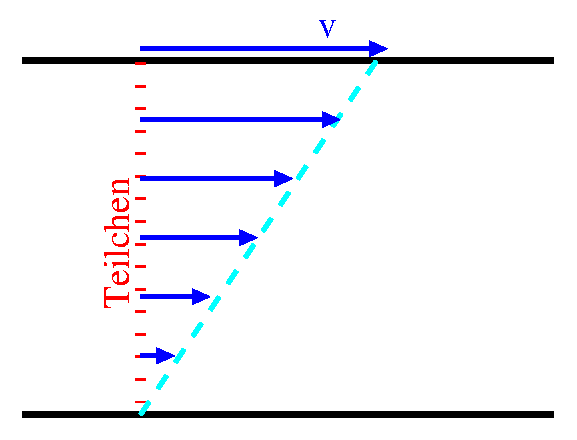
\includegraphics[width=0.3\textwidth]{bilder/lineare-stroemung}\label{abb_linaers-geschwindigkeisprofil}}
\subfigure[Quadratische Str"omung im Rohr]{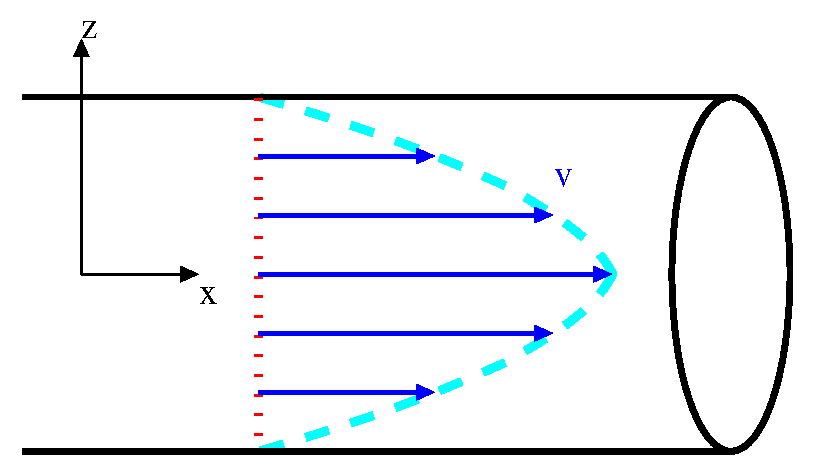
\includegraphics[width=0.3\textwidth]{bilder/quadratische-stroemung}\label{abb_quadratisches-geschwindigkeitsprofil}}
\caption[Geschwindigkeitsprofile von
Flüssigkeiten]{Geschwindigkeitsprofile}
   \label{abb_geschwindigkeitsprofile}
\end{figure}



\subsection{Str"omungsmechanik f"ur z"ahe Fl"ussigkeiten: Laminare Str"omungen}
\label{kap_stromungsmechanik-fur-zahe-flussigkeiten}

\subsubsection{Strom und Widerstand}
\label{kap_strom-und-widerstand}



\begin{Def}
   [\index{Stromst"arke}Stromst"arke $I$] ist die "Anderung des
   (Fl"ussigkeits)Volumens am Ort; also die Differenz aus an- und
   abflie"sender Fl"ussigkei pro Zeiteinheit.
   \begin{equation}
      \label{eqn_def_stromstaerke}
      I = \frac{\Delta V}{\Delta  t} \to \frac{\diff V}{\diff t} =
      \dot V
   \end{equation}
\end{Def}
mit der Einheit $[I] = \frac{m^3}{s}$.

Damit ein Strom flie"st\footnote{die Terminologie ist hier bewusst an
  die der Elektrodynamik angelehnt -- schlie"slich kann man viele
  Zusammenh"ange zwischen diesen beiden Disziplinen feststellen...},
braucht es im betreffenden Leiter einen \emph{Druckunterschied}: Die
Fl"ussigkeit wird dann von Stellen h"oheren Drucks an Stellen
niedrigeren Drucks bewegt: Wenn auf der linken Seite eines Rohres ein
h"oherer Druck herrscht, so kann man sich die Kr"afte auf ein
Wasserteilchen anschauen. Diese m"ussen insgesamt nach rechts zeigen,
weil die Kraft von links (da $F \sim p$ d"urfen wir hier nicht nur von
niedrigerem Druck sondern auch von kleinere Kraft sprechen) schw"acher
ist.

Es gilt der Zusammenhang:
\begin{Wichtig}
   [Stromst"arke -- Druckdifferenz]
Nach \textsc{Haagen-Poiseuille} gilt: Der Stromfluss $I$ ist
proportional zur Druckdifferenz.
\begin{equation}
   \label{eqn_stromstaerke-bei-druckdifferenz}
   I = \frac{p_1 - p_2}{R} = \frac{\Delta p}{R}
\end{equation}
\end{Wichtig}
Dabei hat der Proportionalit"atsfaktor $R$ eine physikalische Bedeutung:
\begin{Def}
   [\index{Str"omungswiderstand}Str"omungswiderstand $R$]
   \begin{equation}
      \label{eq:71}
\boxed{ R = \frac{\Delta p}{I}}
   \end{equation}
\end{Def}
Mit der Einheit $[R] = \frac{\operatorname{Pa} \cdot \operatorname{t}}{\operatorname{m}^3}$.
Er ist abh"angig von 
\begin{itemize}
\item Fl"ussigkeit (also \emph{welche} Fl"ussigkeit str"omt "uberhaupt)
\item Rohrdurchmesser
\item von Geometrie des Rohres (ob es rund, eckig ... ist)
\end{itemize}
Es gilt f"ur ein \textbf{rundes langs Rohr}:
\begin{Wichtig}
   [Gesetz von
   \textsc{\index{Hagen-Poiseuille}\index{Hagen}Hagen-\index{Poiseuille}Poiseuille}]
   Die Stromst"arke ist zur Druckdifferenz proportional (nach
   Gl. \eqref{eq:71}) mit
\begin{equation}
   \label{eq:70}
   \frac{1}{R} = \frac{\pi}{8} \cdot \frac{r^4}{\eta \cdot L}
\end{equation}   
\end{Wichtig}
Wobei $r$ der Radius des Rohres, $L$ die durchstr"omte L"ange und
$\eta$ die Viskosit"at. Man erh"alt es, indem man die Reibungskraft aus
\eqref{eqn_def_viskositaet} mit der Kraft gleichsetzt, welche die
Str"omung erzeugt: $F = A \cdot \Delta p = \pi r^2 \Delta p$.


\subsubsection{Verschaltung von Rohren}
\label{kap_verschaltung-von-rohren}


Wir k"onnen verschiedene Leitungen auf zwei verschiedene Arten
zusammenschalten:
\begin{description}[\setlabelstyle{\bfseries\slshape}]
\item[\index{Reihenschaltung}Reihenschaltung] Die Widerst"ande
   summieren sich, die Stromst"arke muss konstant bleiben:
$$
R_{ges} = \sum_i R_i
$$

\item[\index{Parallelschaltung}Parallelschaltung]
Die reziproken der Widerst"ande addieren sich, die Stromst"arke addiert
sich direkt:
$$I_{ges} = \sum_i I_i$$
$$R_{ges} = \left ( \sum_i \frac{1}{R_i} \right )^{-1}$$
\end{description}
F"ur (analoge) Herleitungen siehe
Kap. \ref{kap_stromkreis-und-schaltungen} auf
S. \pageref{kap_stromkreis-und-schaltungen}.

\begin{figure}
   \centering
\subfigure[Reihenschaltung]{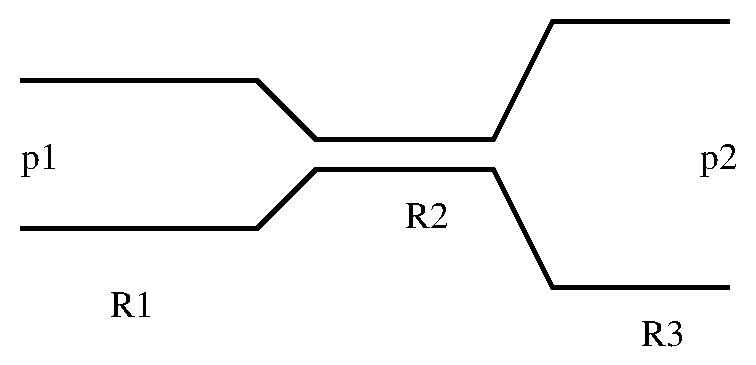
\includegraphics[height=0.1\textheight]{bilder/rohre_reihe}\label{abb_rohre_reihe}}   
\subfigure[Parallelschaltung]{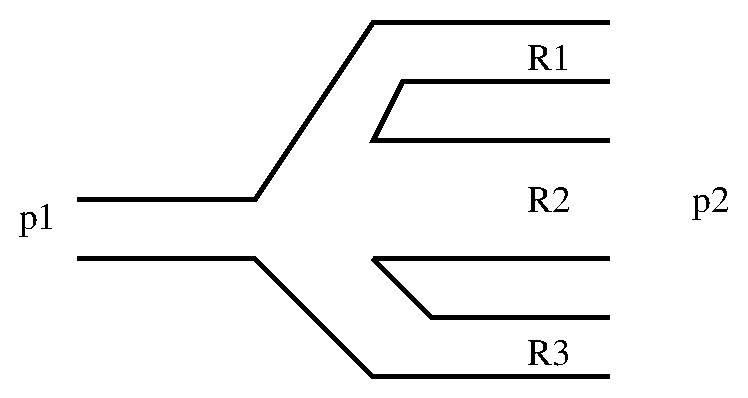
\includegraphics[height=0.1\textheight]{bilder/rohre_parallel}}
   \caption{Schaltungen von Rohren}
   \label{abb_rohre_schaltungen}
\end{figure}


\subsubsection{Festk"orper in Fl"ussigkeit}
\label{kap_festkorper-in-flussigkeit}

\begin{Wichtig}
   [\index{Stokes-Reibung}\textsc{Stokes}-Reibung]
Eine Kugel mit Radius $r$ erf"ahrt die geschwindigkeits($v$)abh"angige Reibung
\begin{equation}
   \label{eq:76}
   F_R = 6 \, \pi \, \eta \, r \cdot v
\end{equation}
\end{Wichtig}
Trotzdem sinken Kugeln mit gro"sem Radius schneller. Das liegt daran,
dass sie einen kleineren Auftrieb haben. Wir betrachten dazu eine
unbeschleunigte Kugel, die mit der konstanten Geschwindigkeit $v_0$ f"allt:
$$
F_G - F_A - F_R = 0 ~ ~\Rightarrow F_G - F_A = F_R
$$
wobei wir die nach unten weisenden Kr"afte als positiv ansehen. Setzen
wir \eqref{eq:61} und \eqref{eq:76} ein, erhalten wir:
\begin{eqnarray*}
   \label{eq:77}
   \varrho_\text{Kugel} \cdot g \cdot V - \varrho_\text{Fl} \cdot g
   \cdot V &=& 6\pi\eta r \cdot v_0 \\
   (\varrho_\text{Kugel} - \varrho_\text{Fl}) \cdot g
   \cdot \frac{4}{3}\pi r^3  &=& 6\pi\eta r \cdot v_0 
\end{eqnarray*}
\begin{equation}
   \label{eq:78}
   v_0 =  (\varrho_\text{Kugel} - \varrho_\text{Fl}) \cdot g \cdot
\frac{4 \pi r^3}{3 \pi \eta r} = (\varrho_\text{Kugel} -
\varrho_\text{Fl}) \cdot g \cdot \frac{4 r^2}{3 \eta}
\end{equation}
also der Zusammenhang
\begin{equation}
   \label{eq:79}
   v_o \sim \frac{r^2}{\eta}
\end{equation}

Diesen Sachverhalt k"onnen wir f"ur die \emph{Viskosit"atsbestimmeung} mit
\emph{\index{Kugelfallviskosimetern}Kugelfallviskosimetern} verwenden;
hier kann man aus $v$ $\eta$ errechnen.

\begin{Def}
   [\textsc{Newton}'sche Fl"ussigkeit]
Wir nennen eine Fl"ussigkeit \textsc{Newton}'sch, wenn gilt
\begin{equation}
   \label{eq:80}
   v \sim \frac{1}{\eta}
\end{equation}
\end{Def}









\subsection{Ideale Fl"ussigkeit}
\label{kap_ideale-flussigkeit}

Wo bei den z"ahen Fl"ussigkeiten die Reibungskr"afte noch ausschlaggebend
waren, k"onnen wir diese jetzt vernachl"assigen.

Wir betrachten bspw. ein gef"ulltes Rohr mit Druckunterschied an den
beiden Enden. Die Fl"ussigkeit wird vom Bereich hohen Drucks zum
Bereich niedrigen Drucks flie"sen. Wenn jetzt aber zwischen den beiden
Enden noch eine \emph{Verj"ungung} im Rohr ist, so wird hier der Druck
\emph{kleiner} sein, als an den beiden Rohrenden
(vgl. Abb. \ref{abb_rohr_verjuengung}). Trotzdem wird die Fl"ussigkeit
weiterflie"sen.

Wir betrachten dazu ein bestimmtes Volumen $\Delta  V$ in den drei
verschiedenen Rohrabschnitten. Die \emph{Stromst"arke} muss dabei
konstant bleiben: 
\begin{equation}
   \label{eq:81}
   I = \frac{\Delta V}{\Delta t} = \frac{\diff V_i}{\diff t} = \frac{A_i \cdot \diff s_i}{\diff t} =
A_i \cdot v_i = \const
\end{equation}
Daraus k"onnen wir folgern:
\begin{itemize}
\item je kleiner das Rohrdurchmesser $A_i$ ist, desto gr"o"ser ist die
   entsprechenden Geschwindigkeit $v_i$.
\item Die Kinetische Energie "andert sich beim Fluss:
   \begin{equation}
      \label{eq:82}
      \Delta E_{kin} = \frac{1}{2} \underbrace{\varrho \cdot \Delta
        V}_{\Delta M} ( v_2^2 - v_1^2 )
   \end{equation}
\end{itemize}

Andererseits m"ussen wir beachten, dass beim Str"omen die Arbeit
("`Volumenarbeit"') verrichtet wird:
\begin{equation}
   \label{eq:83}
   W =  \int F \diff s \stackrel{\const}{=} F \cdot s = \underbrace{p \cdot A}_F
   \cdot s = p \cdot V
\end{equation}
und damit
\begin{equation}
   \label{eq:84}
   \Delta W = (p_1 - p_2) \cdot \Delta V
\end{equation}
dies entspricht einer \textbf{potentiellen} Energie: Die Energie, die
aufgebracht werden muss, um den Druck von $p_1$ auf $p_2$ zu
"andern. Nach dem Energieerhaltungssatz muss nun gelten $\Delta W =
\Delta E_{kin}$ und mit Gl. \eqref{eq:82} und \eqref{eq:84}:
\begin{equation}
   \label{eq:85}
   \frac{1}{2} \underbrace{\varrho \cdot \Delta
     V}_{\Delta M} ( v_2^2 - v_1^2 )  = (p_1 - p_2) \cdot \Delta V   
\end{equation}
und man erh"alt durch Umformung:
\begin{equation}
   \label{eq:86}
  \frac{1}{2} \cdot \varrho \cdot v_2^2 + p_2 = \frac{1}{2} \cdot
   \varrho \cdot v_1^2 + p_1 
\end{equation}
und diese Formel ist an beliebigen Stellen g"ultig! Wir bezeichnen sie
als:
\begin{Wichtig}
   [\textsc{\index{Bernulli-Gleichung}Bernulli}-Gleichung] f"ur
   horizontal str"omende, ideale Fl"ussigkeiten:
   \begin{equation}
      \label{eq:87}
        \underbrace{\frac{1}{2} \cdot \varrho \cdot
          v^2}_\text{Staudruck} + \underbrace{p}_\text{hydrostatischer
        Druck} =  p_{ges} = \const
   \end{equation}
\end{Wichtig}
Dabei ist der hydrostatische Druck der von einem Barometer messbare
Druck.
\begin{figure}
   \centering
   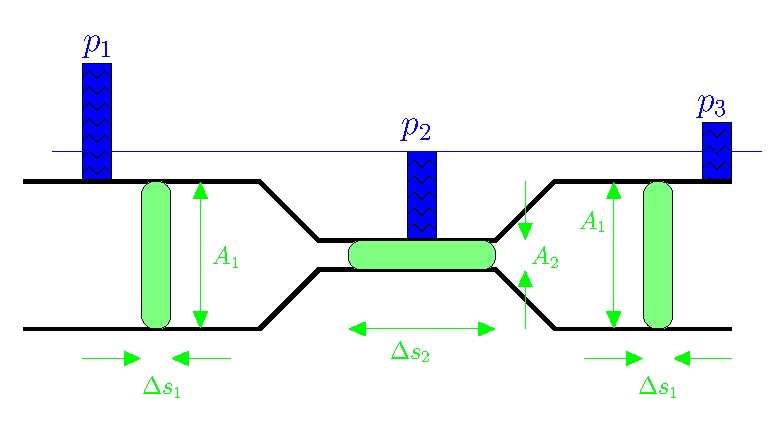
\includegraphics[width=0.7\textwidth]{bilder/rohr_verjuengung}
   \caption[Ideale Flüssigkeit in untersch. dickem Rohr]{Ein Rohr
     mit Verj"ungung, gef"ullt mit einer idealen Fl"ussigkeit. Gr"un
     ist ein einheitliches Volumen in den Drei Rohrabschnitten, blau
     ist der Druck -- also eine Wassers"aule, die man im Experiment
     sehen k"onnte.}
   \label{abb_rohr_verjuengung}
\end{figure}



\subsection{Anwendungen bei idealen Fl"ussigkeiten}
\label{kap_anwendungen-bei-idealen-flussigkeiten}

Ein paar Anwendungen:
\begin{Beispiel}
\begin{enumerate}[(i):]
\item \textbf{\index{Zerst"auber}Zerst"auber /
     \index{Wasserstrahlpumpe}Wasserstrahlpumpe}: Durch ein Rohr wird
   ein Fluid geschickt. An einer Verj"ungung ist ein zweites Rohr
   angeschlossen. An dessen Ende setzt man die zu zerst"aubende
   bzw. anzupumpende Substanz. Dadurch, dass das Fluid an der engeren
   Stelle schneller flie"sen muss, ist der Druck hier sehr klein und
   die Stoffe werden angesaugt und in den allgemeinen Strom des Rohres
   beigemischt.

\item \textbf{\index{Pradoxon}Pradoxon}:
%  Wenn man einen Ball unten an eine Platte h"alt
%    und \emph{von oben} Luft herunterbl"ast, f"allt der Ball nicht
%    herunter: Die Luft umstr"omt den Ball und muss
   Setzt man einen Ball in einen umgest"ulpten Trichter und pustet von
   oben in diesen Trichter, so f"allt der Ball nicht herunter (wenn er
   leicht genug ist).

   Die Luft Umstr"omt den Ball und braucht dabei eine l"angere Strecke
   (weil der Ball rund ist). Folglich ist sie schneller und damit ist
   hier der Luftdruck klein. Zwischen Trichter und Ball ist der
   Luftdruck so klein, dass der Ball an die Trichterwand gezogen wird.

\item \textbf{\index{Bananenflanke}Bananenflanke}: Wenn ein Ball von
   einer schiefen Ebene in ein Wasserbecken f"allt, so wird er hier
   nicht seinen Weg geradlienig fortsetzen, sondern eine krumme Bahn
   "`schwimmen"' (vgl. Abb. \ref{abb_banane}).

   Die Fl"ussigkeitsteilchen nahe der Kugel bewegen sich im Wasser mit
   der Kugel -- sie hat noch eine Rotation von ihrem Weg auf der
   Schiefen Ebene. Auf der \emph{rechten} Seite bewegen sich die
   Molek"ule bez"uglich der Kugel besonders schnell, weil sich hier die
   Rotation der Kugel und ihr Herabsinken addieren\footnote{Wenn die
     Kugel herabsinkt, so fallen die Fluidteilchen um sie herum
     \emph{relativ nach oben}.}. Auf dieser Seite ist also $v$ gro"s
   und damit $p$ klein: Die Kugel wird also nach rechts
   "`gesaugt"'. (s. Def. \ref{def_magnuskraft})


\item \textbf{\index{Golfball}Golfb"alle}: Die kleinen Vertiefungen in
   den Golfb"allen sorgen daf"ur, dass der Magnus-Effekt hier
   besonders stark auftritt. Da der Golfschl"ager den Ball schr"ag
   abschie"st und in Rotation versetzt, sorgt so der Magnus-Effekt
   beim Golfball daf"ur, dass dieser nach oben gezogen wird und damit
   weiter fliegt.
\end{enumerate}
\end{Beispiel}

\begin{Def}
   [\index{Magnuskraft}\textsc{Magnus}kraft] 
\label{def_magnuskraft}Die Querkraft, die ein
   rotierender runder K"orper in einem Fluid bzw. einer Str"omung
   erf"ahrt.
\end{Def}

\begin{figure}
   \centering
   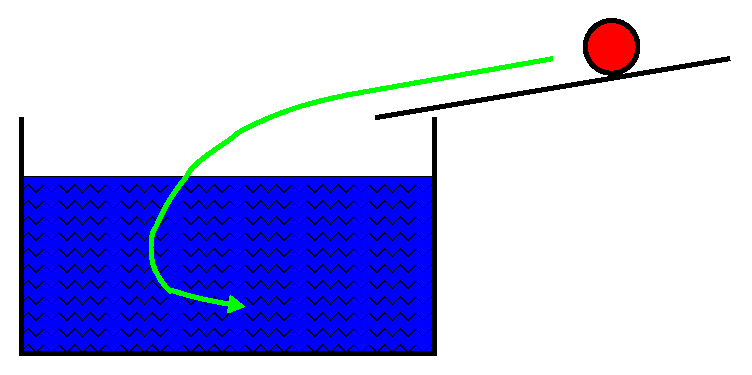
\includegraphics[width=0.5\textwidth]{bilder/banane_traj}
\hfill
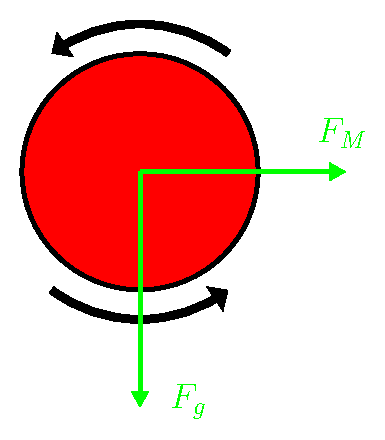
\includegraphics[width=0.3\textwidth]{bilder/banane_vekt}
   \caption{Bananenflanke: Trajektorie und Vergr"o"serung der Kugel}
   \label{abb_banane}
\end{figure}








\subsection{Reale Fl"ussigkeiten}
\label{kap_reale-flussigkeiten}

Wir behandeln schnelle Str"omungen; hier sind die ausschlaggebenden
Gr"o"sen die \emph{Tr"agheitseffekte}. (Die Tr"agheitskr"afte sind weit
gr"o"ser als die Reibungskr"afte.)


Bei kleinen Geschwindigkeiten haben wir geordnete, \emph{laminare}
Str"omungen (vgl. Abb. \ref{abb_geschwindigkeitsprofile}) -- bei
gro"sen Geschwindigkeiten kann es bei realen Fl"ussigkeiten zu
\emph{\index{Turbulenz}turbulenten Str"omungen} kommen, bei denen sich
\emph{\index{Wirbel}Wirbel} bilden.

Diese \textbf{Wirbelbildung} hinter einem Hindernis kann man einfach
dadurch erkl"aren, dass wenn ein Fl"ussigkeitsvolumen an dem Hindernis
vorbeiwandert, seine "au"seren Teilchen direkt am Hindernis
anliegen. Hier wirkt also eine gro"se Reibungskraft auf die
Teilchen. Je weiter weg vom Hindernis -- also "`im Inneren"' des
Fl"ussigkeitsvolumens -- ist die Reibung kleiner, und damit die
Geschwindigkeit gr"o"ser. Da also nahe am Hindernis die
Teilchengeschwindigkeit klein und weit davon entfernt gro"s ist, wird
das Fl"ussigkeitsvolumen eine Rotation bekommen. Durch den
\emph{\textsc{Magnus}-Effekt} (s. Def. \ref{def_magnuskraft}) wird es
dann schlie"slich hinter das Hindernis gezogen: Ein erster kleiner
Wirbel ist entstanden.

Bei gro"sen Geschwindikgeiten kann es nun auch dann zu Wirbeln kommen,
wenn gar keine Hindernisse im Weg waren: Das kommt dann von der
Geschwindigkeits\emph{fluktuation} der Teilchen des
Fl"ussigkeitsvolumens.

\bigskip

Um zu entscheiden, ob eine Str"omung turbulent oder laminar ist, m"ussen
wir unterscheiden ob Tr"agheits- (turbulent) oder Reibungskr"afte
(laminar) die Oberhand haben; daf"ur untersuchen wir den Quotienten
\begin{equation*}
   \label{eq:89}
   \frac{F_\text{Tr"agheit}}{F_\text{Reibung}}
\end{equation*}
und untersuchen die beiden Kr"afte separat:
\begin{description}[\setlabelstyle{\bfseries\slshape}]
\item[Tr"agheit] Ein bewegter K"orper "ubertr"agt Impuls auf Fl"ussigkeit:

Eine Kugel mit Radius $a$ "uberstreicht in $\diff t$ das Volumen $A
\cdot \diff s$. 
Dabei gilt f"ur die Bewegte Menge (Masse) Fl"ussigkeit:
\begin{equation}
   \label{eq:90}
   \frac{\diff m}{\diff
  t} = \varrho \cdot \frac{\diff V}{\diff t} = \varrho \cdot A \cdot
\frac{\diff s}{\diff t} = \varrho \cdot A \cdot v
\end{equation}
Nun muss jedes Teilchen dieser Masse wegbewegt werden. Da wir hier die
Reibung noch au"sen vor lassen, ist dazu lediglich die (Tr"agheits)Kraft 
\begin{equation}
   \label{eq:92}
      F = \frac{\diff p}{\diff t} = \dot p
\end{equation}
 n"otig mit $p = m \cdot v$.
Es gilt:
\begin{equation}
   \label{eq:91}
   \frac{\diff p}{\diff t} = \frac{\diff m \cdot v}{\diff t} +
   \frac{m \cdot \diff v }{\diff t}
\end{equation}
Da wir die Geschwindigkeit hier als konstant ansehen, verschwindet der
zweite Summand. Setzen wir nun also Gl. \eqref{eq:90} in \eqref{eq:91}
und dies in \eqref{eq:92} ein, so erhalten wir:
\begin{equation}
   \label{eq:93}
   F = F_\text{Tr"agheit} = \varrho \cdot A \cdot v^2 = \varrho \cdot
   \pi a^2 \cdot v^2
\end{equation}


\item[Reibung] Die Reibung innerhalb der Fl"ussigkeit ist nach
   Gl. \eqref{eq:76}:
   \begin{equation*}
      F_\text{Reibung} = 6 \pi \eta a \cdot v
   \end{equation*}
   Dabei gilt diese Formel \emph{eigentlich} f"ur ein K"ugelchen des
   Radius $a$. \emph{Eigentlich} m"ussten wir hier f"ur die Herleitung
   die unhandliche
   \textsc{\index{Navier-Stokes-Gleichung}Navier-Stokes}-Gleichung
   verwenden;
   \begin{equation}
      \label{eq:21}
      \varrho \left ( \frac{\partial }{\partial t} + \vec v \cdot \vec
         \nabla \right ) \vec v = -\vec\nabla p + \varrho \cdot \vec g
            + \eta \cdot  \Delta \vec v
   \end{equation}
   wobei $\vec v$ die Bewegung der Teilchen und $\vec g$ die
   Schwerebeschleunigung darstellt. (Die rechte Seite der Gleichung
   beschreibt Kr"afte (das $\Delta$ ist der \emph{Laplace}-Operator)
   und die linke Seite die dadurch hervorgerufene Bewegung.) F"ur
   unsere Zwecke ist die empirisch gefundene \textsc{Stokes}-Reibung
   aber gut genug. (Deshalb haben wir aber in \eqref{eq:94} rechts
   auch keine \emph{Gleichheit}, sondern nur eine \emph{Proportionalit"at}.)
\end{description}
Nun k"onnen wir also den Quotienten bilden:



\begin{Def}
   [\textsc{\index{Reynoldszahl}Reynolds}zahl]
Ein Ma"s, ob eine Str"omung laminar ($R_e < 1$) oder turbulent ($R_e \gg
1$) ist:
\begin{equation}
   \label{eq:94}
R_e =   \frac{F_\text{Tr"agheit}}{F_\text{Reibung}} 
=
    \frac{\varrho \cdot d \cdot v}{\eta} 
\sim
 \frac{\varrho \cdot \pi a^2 \cdot v^2}{6 \pi \eta a v}
\end{equation}
hier ist $d$ der Str"omungsdurchmesser des Gegenstandes.
\end{Def}

Hier flie"st ein: Wenn die Reibung wichtiger ist, ist der Nenner
gr"o"ser, damit die Zahl $R_e$ klein ($R_e < 1$) und damit k"onnen wir
die Betrachtungen aus Kap. \ref{kap_zahe-flussigkeiten}
verwenden. Wenn dagegen die Tr"agheitskr"afte einen entscheidenden
Einfluss bekommen, so wird der Bruch sehr gro"s und wir erhalten
Wirbel.

Da aber auch der Radius $a$ in der Formel auftaucht, k"onnen wir sagen,
dass f"ur kleine $a$ im Normalfall $R_e < 1$.


\begin{Beispiel}
   \textbf{Ruder vs Propeller:} Wenn sich ein kleines Objekt ($a$
   klein \Impl $R_e$ klein \Impl z"ahe Fl"ussigkeit) in einer
   Fl"ussigkeit fortbewegen will, so kann es nicht "`rudern"', weil es
   beim Vorziehen der Ruder wieder die Strecke zur"uckbewegt w"urde,
   die es beim Zur"uckziehen der Ruder vorw"arts gekommen ist. Das
   kleine Objekt braucht einen \emph{Propeller}.

   \textbf{Im Windkanal:} Damit man ein Modell unter realistischen
   Bedingungen testen kann, muss man in Windkan"alen den Druck (und
   damit die Dichte $\varrho$) so anpassen, dass die
   \textsc{Reynolds}zahl in Experiment und Realit"at "ubereinstimmt.
\end{Beispiel}
























%%%%%%%%%%%%%%%%%%%%%%%%%%%%%%%%%%%%%%%%%%%%%%%%%%%%%%%%%%%%%%%%%

%%%%%%%%%%%%%%%%%%%%%%%%%%%%%%%%%%%%%%%%%%%%%%%%%%%%%%%%%%%%%%%

%%%%%%%%%%%%%%%%%%%%%%%%%%%%%%%%%%%%%%%%%%%%%%%%%%%%%%%%%%%%%%%%




 \chapter{Schwingungen und Wellen}
\label{kap_schwingungen-und-wellen}




\section{Freie Schwingung}
\label{kap_freie-schwingung}

\begin{Def}
   [Freie Schwingung]\index{freie Schwingung} Bei einer \textbf{freien
     Schwingung} treten keine externen Kr"afte auf.
\end{Def}

Die hier auftretenden Kr"afte sind stets
\begin{itemize}
\item Die tr"age Kraft $F_T = m \ddot x$
\item eine \emph{lineare} R"uckstellkraft.
\end{itemize}
Je nach \emph{Art} des Pendels (vgl. Abb. \ref{abb_pendel}) unterscheiden sich die R"uckstellkr"afte:
\begin{description}[\setlabelstyle{\bfseries\slshape}]
\item[\index{Federpendel}Federpendel] Federkraft\footnote{Das "`$-$"'
     kommt daher, dass wenn die Auslenkung $x$ (oBdA) in die positive
     Richtung geht, die Federkraft in die \emph{Gegenrichtung} -- also
     in die negative Richtung -- zeigt.}: $F_R = - D \cdot x$
\item[\index{Torsionspendel}Torsionspendel] Federkraft\footnote{mit
     der \emph{Federrichtgr"o"se} $D^*$, mit $D^* :=
     \frac{F}{\varphi}$} $F_R = -D^* \cdot \varphi$ (hier ist $F_T = I
   \ddot \varphi$)
\item[\index{Fadenpendel}Fadenpendel] $F_R = -F_G \cdot \sin \varphi =
   -mg \cdot \sin \varphi \approx -mg \cdot \varphi$
\end{description}

Da hier keine externen Kr"afte angreifen, muss sich die Tr"age Kraft
$F_T$ komplett aus der R"uckstellkraft ergeben\footnote{Dass die Tr"age
  kraft vorhanden sein muss, ergibt sich daraus, dass ein Pendel
  st"andig seine Geschwindigkeit "andert. So muss st"andig eine
  Beschleunigung wirken und mit $F = ma$ muss damit st"andig eine Kraft
  wirken.} -- schlie"slich ist keine andere Kraft da:
\begin{equation}
   \label{eq:101}
   F_T = F_R
\end{equation}
Am Beispiel des Federpendels gilt dann:
\begin{equation}
   \label{eqn_freie-schwingung}
   m\ddot x = - D x ~ \Leftrightarrow ~ \boxed{m\ddot x + Dx = 0}
\end{equation}
Dies ist die verallgemeinerte \textbf{Bewegungsgleichung} einer freien
Schwingung!

Hier haben wir stets eine \emph{Differentialgleichung} zu l"osen -- wir
haben $x(t)$ zu bestimmen. Hier hilft der Ansatz
\begin{equation}
   \label{eq:103}
   x(t) = \hat x \cdot \sin(\omega t + \varphi_0)
\end{equation}
\begin{Def}
   \label{def_harmonische-schwingung} Wir bezeichnen eine Schwingung
   als \textbf{\index{harmonische Schwingung}harmonische Schwingung}, wenn der Systemparameter (die
   Koordinate) einer \emph{Sinusfunktion} in der Zeit folgen kann.
\end{Def}
Durch Ableiten und Einsetzen erh"alt man hierbei mit \eqref{eqn_freie-schwingung}:
\begin{equation}
   \label{eq:104}
   \omega = \sqrt{\frac{D}{m}}
\end{equation}
und damit eine Schwingfrequenz von 
\begin{equation}
   \label{eq:105}
   \nu = \frac{1}{T} =  \frac{\omega}{2\pi} = \frac{\sqrt{D}}{2\pi \sqrt{m}} 
\end{equation}
Die Gleichungen f"ur die anderen Schwingungen lassen sich analog l"osen.


\begin{figure}
   \centering
   \subfigure[Torsionspendel]{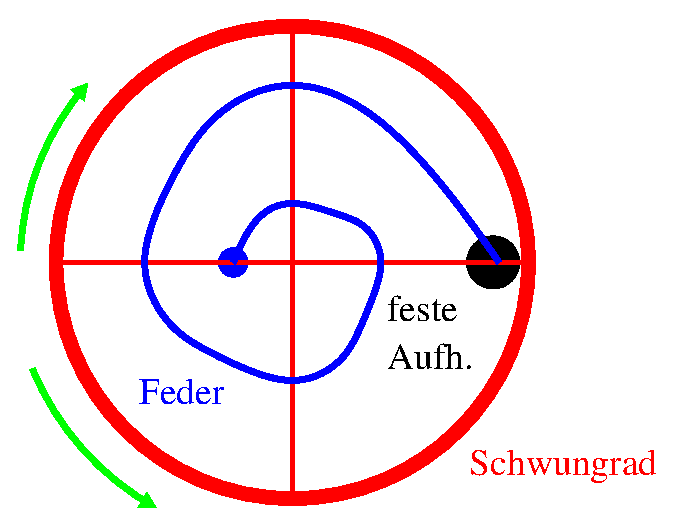
\includegraphics[width=0.3\textwidth]{bilder/torsionspendel}}
   \subfigure[Federpendel]{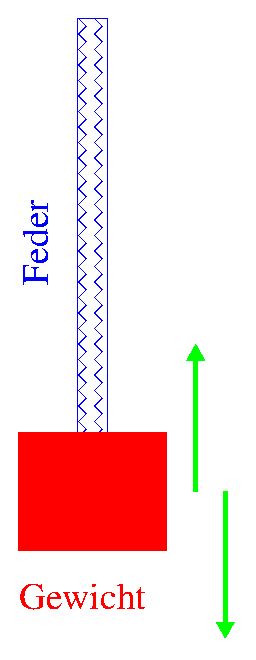
\includegraphics[height=0.22\textheight]{bilder/federpendel}} 
   \subfigure[Fadenpendel]{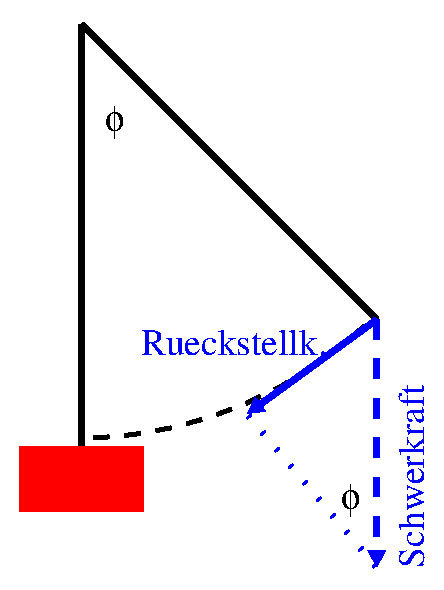
\includegraphics[width=0.3\textwidth]{bilder/fadenpendel}}
   \caption{Verschiedene Sorten von Pendeln}
   \label{abb_pendel}
\end{figure}








\section{D"ampfung}
\label{kap_dampfung}

Nun k"onnen neben der R"uckstellkraft und der Tr"agen Kraft noch
weitere Kr"afte angreifen, die wir meistens vernachl"assigen;
bspw. \textbf{\index{Reibung}Reibungskr"afte}. Die Reibung
("`\index{D"ampfung"'}D"ampfung"') ist meistens von der
Geschwindigkeit abh"angig:
\begin{equation}
   \label{eq:102}
   F_D = - \gamma \dot x
\end{equation}

Wir erhalten dann die \textbf{Bewegungsgleichung} wieder, weil sich
die Tr"age Kraft als Summe der andere Kr"afte darstellen l"asst:
\begin{equation}
   \label{eqn_schwingung-reibung}
   F_T = F_R + F_D ~ \Leftrightarrow ~\boxed{ m\ddot x + \gamma \dot x
     + Dx = 0 }
\end{equation}
Wir sprechen dann von einer \textbf{freien ged"ampften Schwingung.}

Diese freie Schwingung ist keine \emph{harmonische Schwingung} mehr!



\subsection{Geratener Ansatz}
\label{kap_geratener-ansatz}



Als Ansatz zum L"osen der
DGL\footnote{\textbf{D}ifferenzial\textbf{gl}eichung} verwenden
(raten)\footnote{Diese Technik wird auch als "`\emph{clever guess}"'
  bezeichnet.} wir
\begin{equation}
   \label{eq:106}
   \boxed{x(t) = \hat x \cdot \exp(-\delta t) \cdot \sin(\omega t + \varphi_0)}
\end{equation}
Durch zweimaliges Ableiten erhalten wir
\begin{equation}
   \label{eq:108}
   \dot x = - \delta \cdot x + \hat x \cdot \omega \cdot \exp(-\delta t) \cdot \cos(\omega t + \varphi_0)
\end{equation}
und 
\begin{equation}
   \label{eq:110}
   \ddot x = (\delta^2 - \omega^2 )\cdot x - 2 \cdot \hat x \cdot \delta \omega \cdot
   \exp(-\delta t) \cdot \cos(\omega t + \varphi_0) 
\end{equation}
und durch Einsetzen in \eqref{eqn_schwingung-reibung} (mit der
Vereinfachung $\theta := \omega t + \varphi_0$):
% \footnote{Dabei
%   steht $\sin$ f"ur $\sin(\omega t + \varphi_0$ und $\cos$
%   entsprechend... $\sin$ ist also hier in gewissem Sinne eine einfache
%   Variable anstatt einer Funktion. }
\begin{equation}
   \label{eq:109}
%    \hat x \exp(-\delta t) 
% \left [
% \delta^2 m - \omega^2 m - 2 \delta \omega m\cos(\omega t +
% \varphi_0) 
% -
% \delta \gamma  \sin(\omega t + \varphi_0) + \omega \gamma 
% \cos(\omega t + \varphi_0)
% +
% D \sin(\omega t + \varphi_0)
%  \right ] = 0
   \hat x \exp(-\delta t) 
\left [
\delta^2 m \sin\theta - \omega^2 m \sin\theta - 2 \delta \omega m\cos\theta
-
\delta \gamma  \sin\theta + \omega \gamma 
\cos\theta
+
D \sin\theta
 \right ] = 0
\end{equation}
Da $\hat x \exp(-\delta t) \neq 0$ ist, k"onnen wir den Teil in eckigen
Klammern umfornem:
\begin{equation}
   \label{eq:111}
 [ \delta^2m - \omega^2m - \delta \gamma + D ] \sin\theta + [-2\delta\omega m +
 \omega \gamma] \cos\theta = 0
\end{equation}
Da Sinus und Cosinus beide Null werden k"onnen, aber nicht
\emph{gleichzeitig} -- die Gleichungen aber für jede Zeit $t$ und
damit jede Phase $\theta$ -- , muss jeder der Terme in eckigen
Klammern verschwinden, weil wenn $\cos\theta = 0$ gilt, verschwindet
der rechte Term und dann muss der linke ebenfalls verschwinden. Weil
an dieser Stelle $\sin\theta \neq 0$ ist, muss nach dem \emph{Satz vom
  Nullprodukt} die Klammer verschwinden; wir erhalten also
\begin{eqnarray}
   \label{eq:112}
    \delta^2m - \omega^2m - \delta \gamma + D  &=& 0\\
\label{eq:113}
-2\delta\omega m +
 \omega \gamma &=& 0
\end{eqnarray}
Aus \eqref{eq:113} gilt 
\begin{equation}
   \label{eq:114}
   \delta = \frac{\gamma}{2m}
\end{equation}
und damit und mit \eqref{eq:112} gilt
\begin{equation}
   \label{eq:115}
\omega^2 =  \frac{D}{m} - \frac{\gamma^2}{4m^2}
\end{equation}
Aus Kap. \ref{kap_freie-schwingung}  wissen wir,
die Frequenz der zugeh"origen \emph{freien Schwingung}:
\eqref{eq:104}. Diese nennen wir hier $\omega_0$. Mit \eqref{eq:114}
gilt also:
\begin{equation}
   \label{eq:116}
\boxed{   \omega = \sqrt{\omega_0^2  -  \delta^2}  }
\end{equation}




\subsection{Allgemeiner Ansatz}
\label{kap_allgemeiner-ansatz}

Der Allgemeine Ansatz zur L"osung einer DGL wie
\eqref{eqn_schwingung-reibung} ist 
\begin{equation}
   \label{eq:119}
  x =    x(t) = c \exp(\lambda t)
\end{equation}
Durch Ableiten 
\begin{eqnarray}
   \label{eq:120}
   \dot x &=& \lambda \cdot x\\
 \ddot x &=& \lambda^2 \cdot x
\end{eqnarray}
und Einsetzen
\begin{equation}
   \label{eq:121}
   m \lambda^2 x + \gamma \lambda x + D x = 0
\end{equation}
kommt man (durch K"urzen mit $x$ da $x \neq 0$ f"ur $c \neq 0$) auf das
\emph{\index{characteristisches Polynom}characteristische Polynom}
\begin{equation}
   \label{eq:122}
    m \lambda^2 + \gamma \lambda + D  = 0
\end{equation}
welches wir mit der Mitternachsformel l"osen k"onnen:
\begin{equation}
   \label{eq:123}
   \lambda = \frac{-\gamma \pm \sqrt{\gamma^2 - 4Dm}}{2m}
 = 
\frac{- \gamma }{2m} \pm \sqrt{\frac{\gamma^2}{4m^2} - \omega_0^2}
=:
- \delta \pm \underbrace{\sqrt{\delta^2 - \omega_0^2}}_{\I \omega}
\end{equation}
Die Allgemeine L"osung f"ur die DGL \eqref{eqn_freie-schwingung} ergibt
sich dann als
\begin{equation}
   \label{eq:124}
   x(t) = c \exp \left (\frac{- \gamma }{2m} \cdot t + \sqrt{\frac{\gamma^2}{4m^2} -  \omega_0^2}  \cdot t\right ) + \bar c \exp \left ( \frac{-
        \gamma }{2m} \cdot t- \sqrt{\frac{\gamma^2}{4m^2}
        - \omega_0^2}  \cdot t\right )
\end{equation}
oder als
\begin{equation*}
x(t) = \left ( c \cdot \exp( \sqrt{\delta^2 - \omega_0^2} \cdot t) + \bar
   c \cdot \exp(- \sqrt{\delta^2 - \omega_0^2}\cdot t)  \right) \cdot
\exp(-\delta \cdot t)
\end{equation*}
\begin{Wichtig}
$\bar c$ ist \emph{komplex konjugiert} zu $c$
\end{Wichtig}
Eigentlich m"ussten wir die beiden Konstanten $c$ und die, wo jetzt
$\bar c$ steht, frei w"ahlen k"onnen. Dadurch, dass wir die komplex
konjugierte w"ahlen, investieren wir Information: Die Schwingung findet
im \emph{reellen} statt: Es w"urde keinen Sinn machen, eine komplexe
Gr"o"se f"ur $x$ zu erhalten. Die einzige M"oglichkeit, zu vermeiden dass
$x \in \mathbb C \backslash \mathbb R$ liegt, ist die zweite,
eigentlich freie Konstante als komplex konjugierte zu w"ahlen.

Alternativ kann man auch argumentieren, dass man eine L"osung findet,
die auch komplex sein darf, so lange sie nur die Differenzialgleichung
l"ost. Nun sind sowohl Real- als auch Imagin"arteil dieser komplexen
L"osung \emph{f"ur sich} L"osungen der DGL. Dieser komplexe Ansatz ist
manchmal einfacher zu rechnen. Man b"u"st auch keine
\index{Freiheitsgrade}Freiheitsgrade ein, weil von $c$ sowohl Real-
als auch Imagin"arteil frei w"ahlbar sind!

\bigskip

\noindent
Jetzt m"ussen wir drei Sonderf"alle unterscheiden:
\begin{enumerate}[F{a}ll I:]
\item $\delta^2 < \omega_0^2$: \textbf{schwache D"ampfung}: Der
   "`Inhalt"' der Wurzel von $\lambda$ ist negativ, also ist $\lambda$
   imagin"ar, was uns auf eine \emph{Schwingung} f"uhrt. Man kann
   $\exp(-\delta t)$ ausklammern und erh"alt\footnote{Setzt man stur
     ein und beachtet, dass $\bar c$ das komplex konjugierte von $c$
     ist, folgt dies direkt.}
   \begin{equation*}
      x(t) = \left(2 \Re c \cos \omega t - 2 \Im c \sin \omega
         t\right)\cdot \E^{-\delta t}
   \end{equation*}
   Diese Darstellung ist aber noch etwas sperrig (mit Sinus \emph{und}
   Cosinus darin). Dazu schreiben wir $c$ und $\bar c$ in der
   Komplexen Exponentenschreibweise um:
\begin{equation}
   \label{eq:20}
   c = |c| \E^{\I \varphi} \text{ und } \bar    c = |c| \E^{- \I \varphi}
\end{equation}
mit dem $\varphi$ von Gl. \eqref{eq:126}. Wir k"onnen so
Gl. \eqref{eq:124} umschreiben\footnote{Da $\I$ kommt daher, dass die
  Wurzel negaitv ist -- das $\omega$ soll aber reell sein, deswegen
  zieht man die $-1$ unter der Wurzel hervor.} zu
\begin{equation}
   \label{eq:2}
 x(t)  =  |c| \cdot \left( \E^{\I (\omega t + \varphi)} + \E^{-\I (\omega t +
        \varphi)}\right) \cdot \E^{-\delta t}
\end{equation}
und das widerum\footnote{Dazu stellt man auf $\E^{\I\phi} = \cos\phi +
  \I\sin\phi$ und das komplex konjugierte ist $\E^{-\I\phi} = \cos\phi
  - \I\sin\phi$. Dann Summiert man diese beiden Terme.} zu
\begin{equation*}
   x(t) =  2|c| \cdot \cos \left(\omega t + \varphi \right) \cdot \E^{-\delta t}
\end{equation*}
und mit eingesetzten Werten:
   \begin{equation}
      \label{eqn_schwache-daempfung}
\boxed{      x(t) = \underbrace{2|c|}_{\hat x} \cdot
      \exp(-{\frac{\gamma}{2m}} \cdot t) \cdot \cos (\sqrt{\frac{\gamma^2}{4m^2} -
        \frac{D}{m}} \cdot t + \varphi ) }
   \end{equation}
   Wobei die Phasenverschiebung $\varphi$ daraus resultiert, dass $c
   \neq \bar c$; dann gilt
   \begin{equation}
      \label{eq:126}
      \varphi = \arctan - \frac{\operatorname{i} (c - \bar c)}{c + \bar
        c} = \arctan \frac{\Im c}{\Re c}
   \end{equation}
Dieses $\varphi$ hat also nicht nur eine mathematische, sondern auch
eine physikalische Bedeutung.

Wir haben also eine Schwingung, die mit $\exp ( -\delta \cdot t )$
abnimmt; man bezeichnet $\delta$ deshalb auch als \textbf{Dekrement}.



\item $\delta^2 > \omega_0^2$: \textbf{starke D"ampfung}: Die Wurzeln
   aus \eqref{eq:123} sind jetzt reell.\footnote{Deswegen sind die
     beiden Konstanten $c_1$ und $c_2$ jetzt auch beide reell (und
     voneinander unabh"angig)!} Wir bezeichnen sie mit $\mu$ und $-\mu$
   und erhalten so als L"osung (nach Ausklammern und Einsetzen von
   $\exp( -\delta t)$):
   \begin{equation}
      \label{eq:127}
      x(t) = \E^{-\delta t} \cdot \left ( c_1\exp( \mu t )+ c_2 \exp (-\mu t) \right )
   \end{equation}
   Wenn wir nun als Anfangsbedingung $x(t = 0) = 0$ annehmen, so gilt
   $c_1 + c_2 = 0$ und wenn wir weiter $\dot x(t = 0) = v_0$ setzen, so
   gilt\footnote{mit dem Ergebnis aus der ersten Anfangsbedingung (Nur
   mit der zweiten Bedingung erh"alt man $\mu(c-1 - c_2) -
   \delta(c_1+c_2) = v_0$. Mit der ersten Bedingung verschwindet der
   $\delta$-Term links.}
   $c_1 - c_2 = \frac{v_0}{\mu}$. Verbindet man nun die Bedingungen
   f"ur $c_1$ und $c_2$ so erh"alt man $2c_1 = \frac{v_0}{\mu}$ und
   $2c_2 = -\frac{v_0}{\mu}$ und so folgt:
   \begin{equation}
      \label{eq:128}
      x(t) = \frac{v_0}{2 \mu} \E^{-\delta t} \cdot ( \exp(\mu t) - \exp(-\mu t))
   \end{equation}
   Dies ist genau die Definition f"ur den Sinushyperbolicus:
   \begin{equation}
      \label{eqn_starke-daempfung}
\boxed{      x(t) = \frac{v_0}{\mu} \exp (- \delta t) \cdot \sinh \mu
  t }
   \end{equation}
   Und mit eingesetzten "`Werten"':
   \begin{equation*}
      x(t) = \frac{v_0}{\sqrt{\frac{\gamma^2}{4m^2} -
        \frac{D}{m}}} \cdot \exp\left({-{\frac{\gamma}{2m}}\cdot t}\right) \cdot \sinh \left( \sqrt{\frac{\gamma^2}{4m^2} -
        \frac{D}{m}} \cdot t \right)
   \end{equation*}

%    Das bedeutet, dass das Pendel genau einmal ausschl"agt und dann
%    immer langsamer wird und stehen bleibt.
   Wir vergleichen nun die Argumente von $\exp$ und $\sinh$. Wegen
    $\delta^2 > \omega_0^2$ k"onnen wir auch
   sagen, dass $\delta > \omega_0$ -- rein vom Sinn her sind sowohl
   D"ampfung als auch Frequenz positive Gr"o"sen. Wir k"onnen so
   absch"atzen (f"ur $\omega_0 > 0$):
   \begin{equation*}
      \sqrt{\delta^2 - \omega_0^2} < \sqrt{\delta^2} = \delta
   \end{equation*}
   Damit ist das Argument des Exp immer (betragsm"a"sig) gr"o"ser. Wenn
   wir dies beachten, dann ist der Bewegungsverlauf allgemein: Der
   Schwinger wird einmal ausgelenkt, erreicht die maximale Auslenkung
   \emph{nicht} und schwingt dann wesentlich langsamer (asymptotisch)
   in die Ruhelage zur"uck.



\item $\delta^2 = \omega_0^2$: \textbf{\index{aperiodischer
       Grenzfall}aperiodischer Grenzfall}: Die Wurzeln in
   \eqref{eq:123} verschwinden. Man h"atte als einzige L"osung f"ur
   das Charactertische Polynom $\lambda = \frac{- \gamma}{2m} =
   -\delta$.

   Als L"osung der DGL \eqref{eqn_schwingung-reibung} erhalten wir
   so\footnote{Wir brauchen noch eine zweite Unbekannte in unserem
     System und daf"ur einen zweiten Term. Diesen erhalten wir, indem
     wir mit $t$ multiplizieren.} 
   \begin{equation}
      \label{eq:130}
      x(t) = c_1 t \cdot \exp ( -\delta t) + c_2 \exp(-\delta t) 
   \end{equation}

   Wollen wir wieder die Anfangsbedingungen $x(t = 0) = 0$ und $\dot
   x(t = 0) = v_0$ verwenden, erhalten wir $c_2 = 0$ und $c_1 = v_0$
   und damit
\begin{equation}
   \label{eq:131}
   x(t) = v_0 t \cdot \exp( - \delta t)
\end{equation}
Die Schwingung geht hier einmal nach au"sen und schwingt sich langsam
in die Ruhelage zur"uck.

Lassen wir das Pendel stattdessen ausgelenkt starten ($x(t = 0) = \hat
x$ und $\dot x(t = 0) = 0$) erhalten wir $c_2 = \hat x$ und $c_1 =
\delta c_2 = \delta \hat x$. Die L"osung sieht dann so aus:
\begin{equation}
   \label{eqn_aperiod-grenzfall}
\boxed{   x(t) = \hat x (\delta t + 1) \exp(-\delta t)}
\end{equation}

\end{enumerate}

In Abb. \ref{abb_daempf} sind die verschiedenen D"ampfungsarten aufgezeichnet.

\begin{figure}[h]
   \centering
   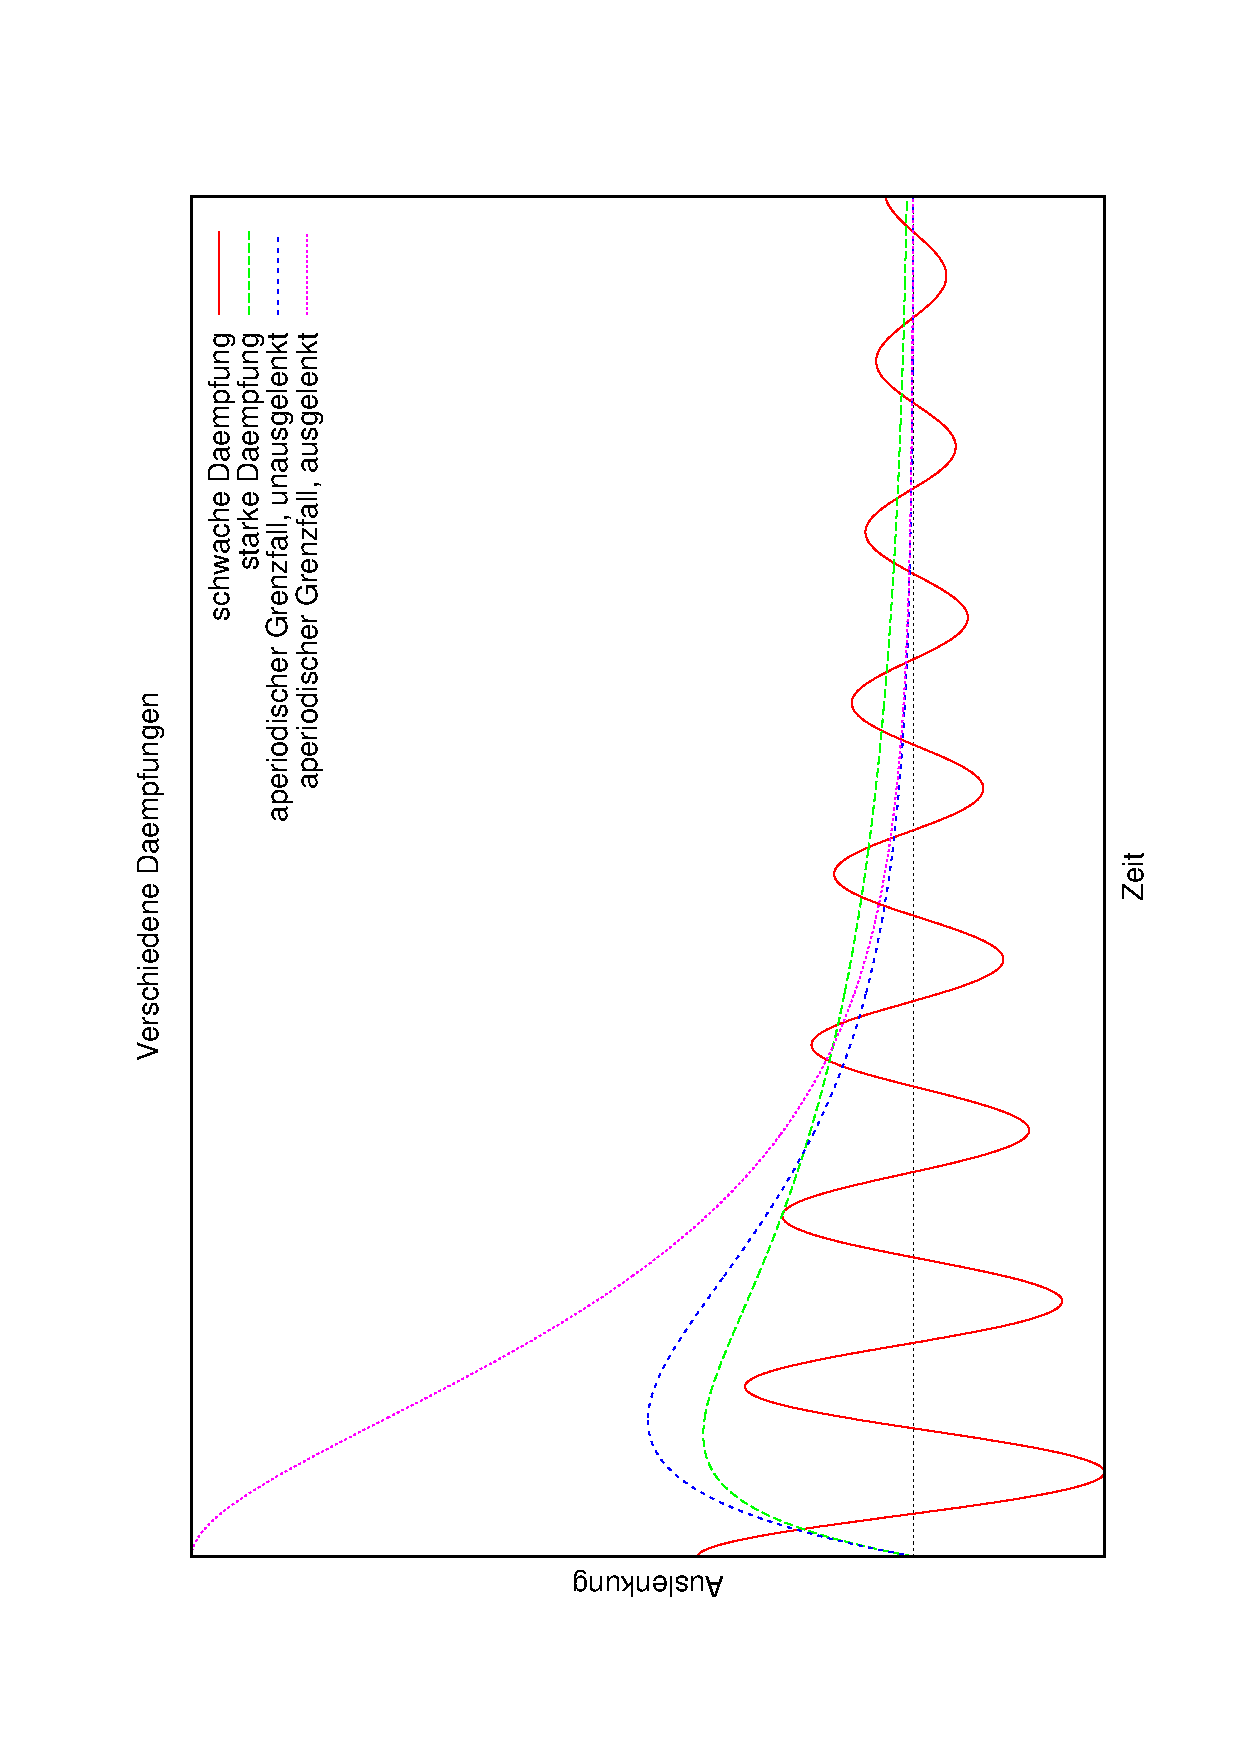
\includegraphics[width=0.7\textwidth,angle=-90]{bilder/dampf01}
   \caption[Dämpfungen einer Schwingung]{Verschiedene D"ampfungen
     einer Schwingung; die Amplituden und Frequenzen wurden
     willk"urlich gew"ahlt.}
   \label{abb_daempf}
\end{figure}









\section{St"orung}
\label{kap_storung}





Nun wollen wir noch eine \textbf{externe Kraft} angreifen lassen:
\begin{equation}
   \label{eq:107}
   F_{ext} = \hat F_{ext} \cos (\omega_{ext} t)
\end{equation}
D.h. unser Pendel wird die ganze Zeit "uber von au"sen periodisch
angeregt. Dem Pendel bleibt nach einer "`Einschwingphase"' nichts
anderes "ubrig, als mit der Frequenz $\omega_{ext}$ zu schwingen. 

Weil periodisch Energie zugef"uhrt wird, wird die D"ampfung praktisch
mit ausgeglichen.

In der \textbf{Bewegungsgleichung} steuert $F_{ext}$ jetzt auch einen Teil
zu $F_T$ bei und wir erhalten analog:
\begin{equation}
   \label{eqn_gestoerte-schwingung}
\boxed{   m\ddot x + \gamma \dot x + Dx = F_{ext} }
\end{equation}




\subsection{\emph{Then-A-Wonder-Occurs}-Ansatz}
\label{kap_then-a-wonder-occurs-ansatz}


Unser neuer \textbf{Ansatz} lautet:
\begin{equation}
   \label{eq:117}
   x(t) = \hat x \sin(\omega_{ext} t + \varphi_{ext})
\end{equation}
Dabei ist $\varphi_{ext}$ die \emph{Phasendifferenz} zuwischen Erreger
und Oszillator (Pendel).

Durch Ableiten und Einsetzen\footnote{Then a wonder occurs} erh"alt man
\begin{eqnarray}
   \label{eq:118}
   \varphi_{ext} &=& \arctan \frac{- \omega_{ext}}{\frac{m}{\gamma}
     (\omega_0^2 - \omega_{ext}^2)}\\
\hat x &=& \frac{\hat F}{\sqrt{(\omega_0^2 - \omega_{ext}^2)^2m^2 +
    {\omega_{ext}^2 \gamma^2}}}
\end{eqnarray}
Siehe dazu Abb. \ref{abb_ampl-erzw}.





\subsection{Allgemeiner Ansatz}
\label{kap_allgemeiner-ansatz-1}


Wir f"uhren $K = \frac{\hat F_{ext}}{m}$ ein, um die DGL
\eqref{eqn_gestoerte-schwingung} umzuformulieren (Achtung: Hier ist
$\delta$ nicht mehr wie oben gew"ahlt!):
\begin{equation}
   \label{eq:125}
   \ddot x + 2 \delta \dot x + \omega_0^2x = K \cos \omega t
\end{equation}
Dann erhalten wir auf der linken Seite die linke Seite von
Gl. \eqref{eqn_schwingung-reibung}. D.h. wir haben hier mit
\eqref{eq:125} eine inhomogene DGL, die wir l"osen, indem wir zu einer
homogenen L"osung (wie \eqref{eq:124} -- oder besser gleich \eqref{eqn_schwache-daempfung}) eine
\emph{\index{Partikul"arl"osung}Partikul"arl"osung} addieren. Diese
Partikul"arl"osung ist nach dem \emph{Ansatz vom Typ der Rechten Seite}
einfach 
\begin{equation}
   \label{eq:129}
   x_p(t) = \hat x_p \cos (\omega_p t + \varphi_p)
\end{equation}
wobei $\omega_p = \omega_{ext} = \omega$ die Erregerfrequenz ist.

D.h. wir erhalten insgesamt als L"osung
\begin{equation}
   \label{eqn_erregt}
\boxed{   x(t) = \hat x_h \exp(-\delta t) \cdot \cos(\omega_h t + \varphi_h)
   + \hat x_p \cdot \cos (\omega_p t + \varphi_p) }
\end{equation}
Wobei  $\omega_h$ die Frequenz der entsprechenden ged"ampften,
\emph{nicht angeregten} Schwingung --
s. Kap. \ref{kap_allgemeiner-ansatz} -- ist.

Wir wollen nun einige \textbf{qualitative Untersuchungen} durchf"uhren:
Da im ersten Term eine exponentiell abnehmende Funktion steckt,
k"onnen wir den ersten Term f"ur gro"se $t$ ignorieren, da $\exp(-t)
\to 0$ f"ur $t \to \infty$ und die Cosinus-Terme beschr"ankt sind.

Nehmen wir an, diese "`\index{Einschwingphase}Einschwingphase"' ist vorbei, dann haben wir
als L"osung nur noch den zweiten Term aus \eqref{eqn_erregt} -- also im
Prinzip \eqref{eq:129}.

Setzen wir diese L"osung in \eqref{eq:125} ein, erhalten wir f"ur $t =
\frac{\pi}{2 \omega_p}$
\begin{equation}
   \label{eq:132}
   \left ( \omega_p^2 - \omega_0^2 \right ) \sin \varphi_p - 2 \delta
   \omega_p \cos \varphi_p = 0
\end{equation}
und damit
\begin{equation}
   \label{eq:134}
 \tan \varphi_p =      \frac{ 2 \delta
   \omega_p}{  \omega_p^2 - \omega_0^2 }
\end{equation}
Und f"ur $t = 0$ gilt:
\begin{equation}
   \label{eq:133}
  \hat x_p \cdot  (\omega_p^2 - \omega_0^2) \cos \varphi_p + 2 \delta
  \hat x_p \omega_p \sin\varphi_p = -K
\end{equation}
Und damit
\begin{eqnarray}
   \label{eq:135}
   \hat x_p \cos \varphi_p &=& \frac{-K - 2 \delta
  \hat x_p \omega_p \sin\varphi_p}{\omega_p^2 - \omega_0^2} \\
\label{eq:136}
\hat x_p \sin \varphi_p &=& \frac{-K - \hat x_p \cdot \left ( \omega_p^2 -
   \omega_0^2 \right ) \cos \varphi_p }{2 \delta \omega_p}
\end{eqnarray}
Da $(\hat x \cos \phi)^2 + (\hat x \sin \phi)^2 = {\hat x}^2$ ist,
k"onnen wir Gl.~\eqref{eq:135} und \eqref{eq:136}  quadrieren und
addieren und erhalten unter Verwendung von \eqref{eq:132}: 
\begin{equation}
   \label{eq:137}
   \hat x_p = \frac{K}{\sqrt{(\omega_0^2 - \omega_p^2)^2 + (2\delta\omega_p)^2}}
\end{equation}













\subsection{F"alle}
\label{kap_falle}



Wir unterscheiden drei verschiedene F"alle f"ur die anregende Frequenz:
\begin{description}[\setlabelstyle{\bfseries\slshape}]
\item[Kleine Frequenzen $\omega_{ext} \ll \omega_0$]
Der Oszillator folgt dem Erreger unmittelbar.

Oszillator und Erreger schwingen in Phase: $\varphi_{ext} =0$ Die
Amplitude f"ur kleine $\omega_{ext}$ ist 
$$
\hat x = \frac{\hat F}{m\omega_0^2} ~\Leftrightarrow ~ \hat F = D \cdot
\hat x
$$

\item["Ahnliche Frequenzen $\omega_{ext} \approx \omega_0$] 
Die Amplitude erreicht ihren H"ochstwert f"ur $\omega_{ext} \equiv
\omega_0$; die Phasenverschiebung geht dann unabh"angig von der
D"ampfung gegen $\varphi_{ext} \to 90^\circ$.

Hier tritt auch die \textbf{\index{Resonanzkatastrophe}Resonanzkatastrophe} ein: Wenn die
D"ampfung $\gamma$ klein genug ist, geht $\hat x \to \infty$.

\item[Hohe Frequenzen $\omega_{ext} \gg \omega_0$] 
Die Amplitude verschwindet.

Der Oszillator kann der Erregung nicht mehr folgen; $\varphi \to 180^\circ$.
\end{description}


\begin{figure}
   \centering
\subfigure[Amplitude im Abh"angigkeit von Anregungsfrequenz]{  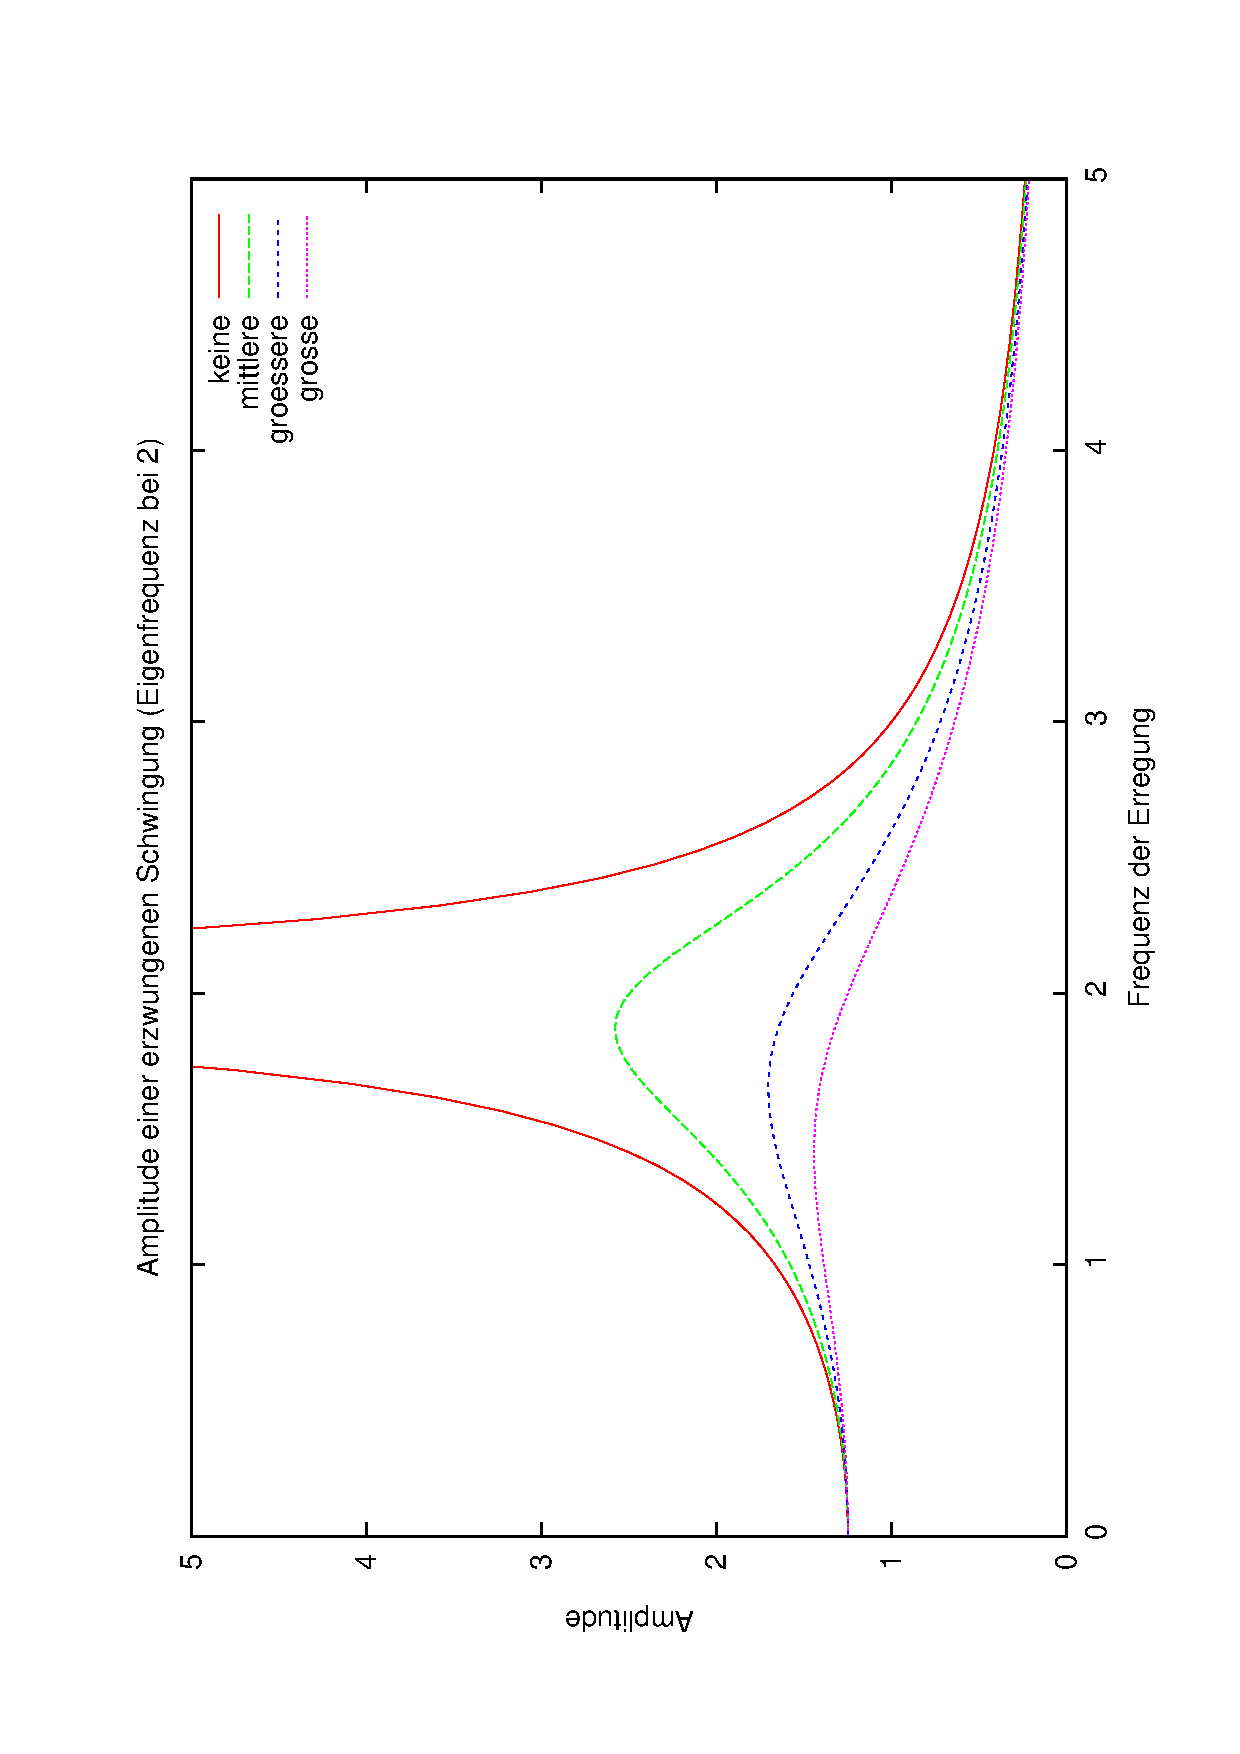
\includegraphics[width=0.8\textwidth,angle=-90]{bilder/ampl-erzw01}} 
\subfigure[Phase in Abh"angigkeit von Anregungsfrequenz]{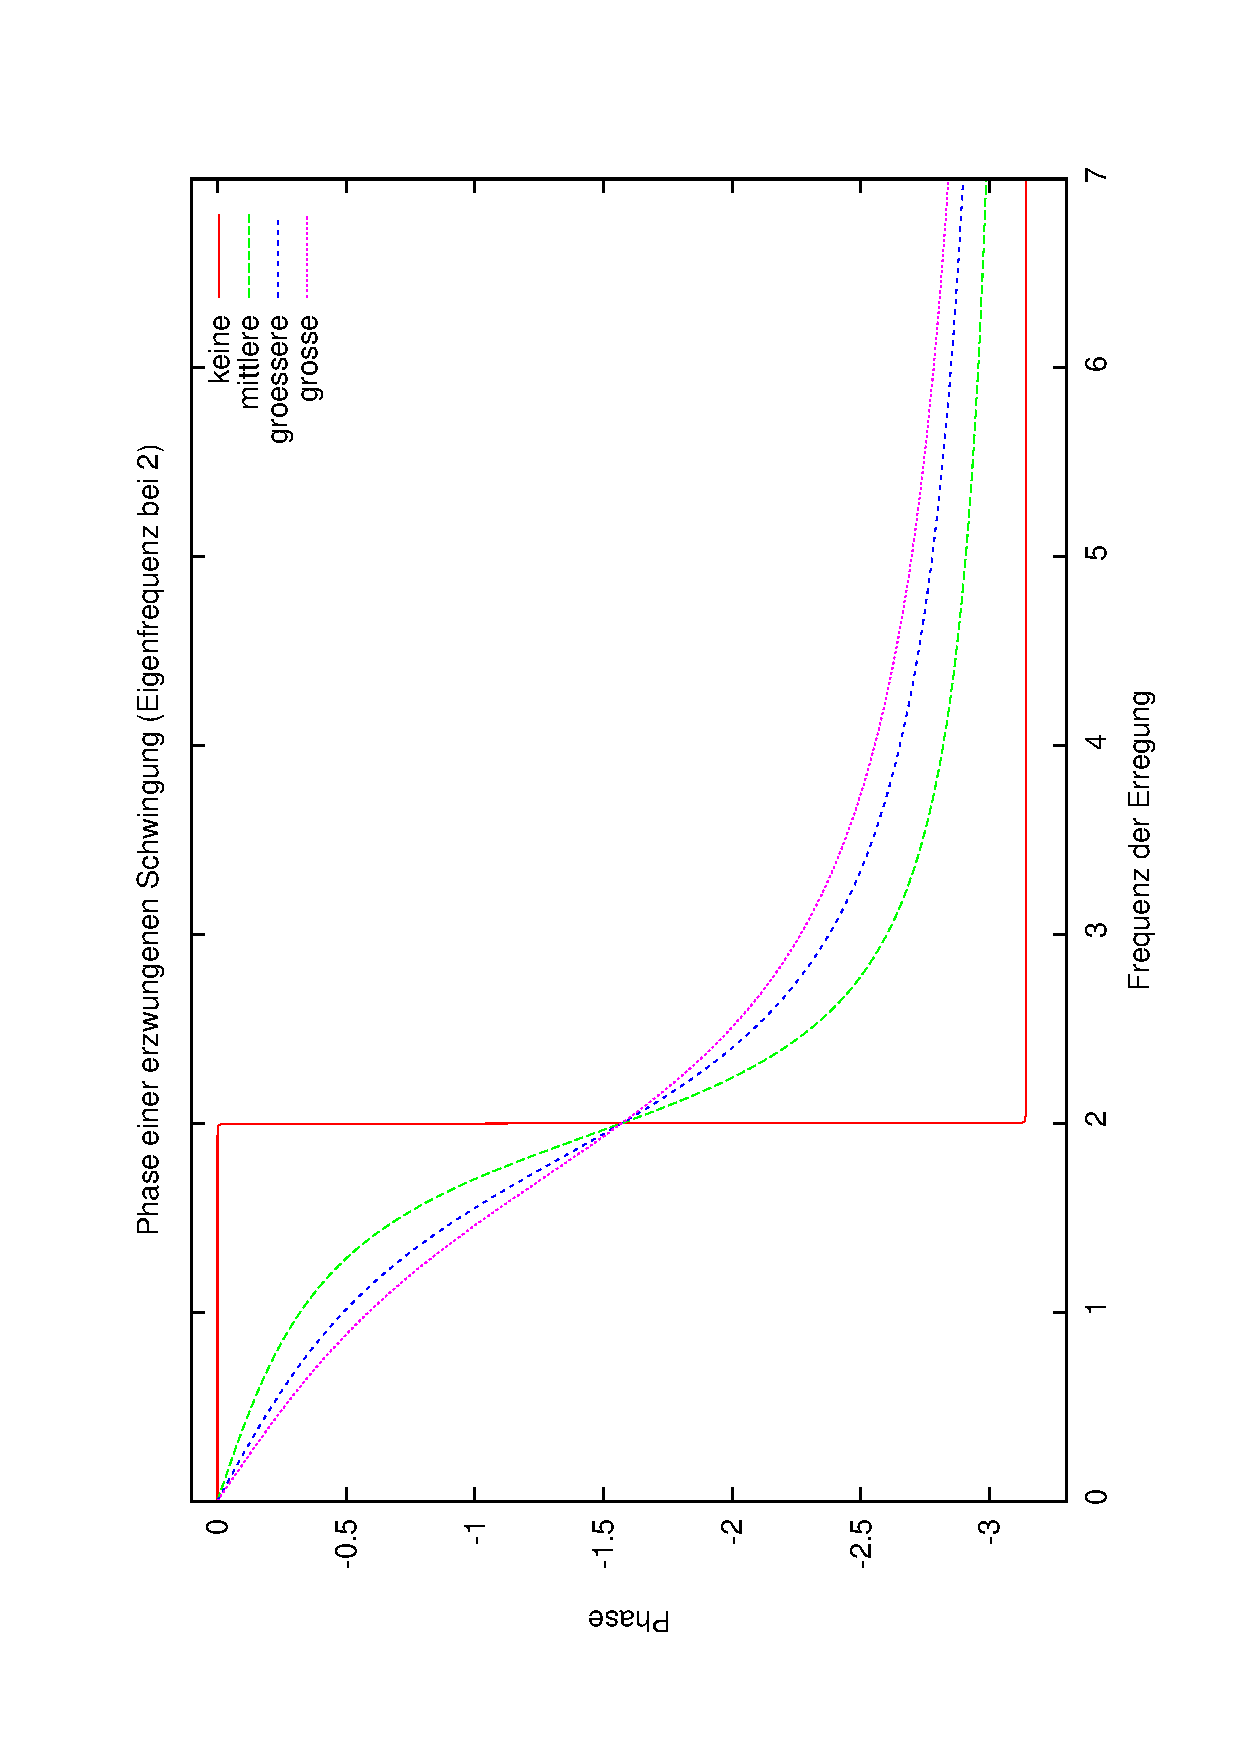
\includegraphics[width=0.8\textwidth,angle=-90]{bilder/phase-erzw01}}
\caption[Amplituden und phasen einer erzwungenen Schwingung]{Amplitude
  und Phase einer Erzwungenen Schwingung bei verschiedenen D"ampfungen
  -- siehe Gl. \eqref{eq:117} \eqref{eq:118}}
   \label{abb_ampl-erzw}
\end{figure}







   





\section{Gekoppelte Schwingungen}
\label{kap_gekoppelte-schwingungen}

Wir lassen zwei Pendel nebeneinander pendeln und verbinden ihre
Gewichte durch eine Feder. Dadurch haben wir zwei (harmonische oder
ged"ampfte) Schwingungen, die von der jeweils anderen Schwingung
angeregt werden. 

Wir f"uhren zwei getrennte Koordinatensysteme ein; das eine Pendel
beschreiben wir mit $x$, das andere mit $y$. Nun "uben die Pendel keine
Kr"afte aufeinander aus, wenn sie gleichphasig (syncron) schwingen;
dann ist der Abstand zwischen ihnen konstant und die Feder wird weder
gedehnt noch gestaucht. Nur wenn die Feder ihre L"ange ver"andert, "ubt
sie eine Kraft auf die beiden Schwinger aus. Die Kraft, die der
\emph{linke} Schwinger erf"ahrt ist\footnote{Lassen wir $x$ konstant
  und vergr"o"sern $y$ so wirkt wirklich eine Federkraft l"angs der
  $x$-Achse auf den linken Schwinger.}
\begin{equation}
   \label{eq:138}
   F_{ext,\text{links}} = D \cdot(y-x)
\end{equation}

D.h. wir k"onnen die Differenzialgleichung der nicht ged"ampften,
angeregten Schwingung aufstellen:
\begin{equation}
   \label{eq:139}
   m \ddot x + Kx = F_{ext} = D(y-x) ~\Leftrightarrow ~ \ddot x +
   \underbrace{\frac{K}{m}}_{\omega_0^2}x + \frac{D}{m}(x-y) = 0
\end{equation}
Dabei verwenden wir $K$ als Konstante f"ur die \emph{R"uckstellkraft}
und $\omega_0$ die Eigenfrequenz des linken Pendels ohne Koppelung.

F"ur den rechten Schwinger gilt entsprechend:
\begin{equation}
   \label{eq:140}
   \ddot y + \omega_0^2 y + \frac{D}{m} (y-x) = 0
\end{equation}


\subsection{Entkoppeln mit Ansatz}
\label{kap_entkoppeln-mit-ansatz}


Als Ans"atze w"ahlen wir hier zwei harmonische Schwingungen:
\begin{equation}
   \label{eq:141}
   x = \hat x \cdot \sin (\omega t + \varphi) ~\text{ und } ~
   y = \hat y \cdot \sin (\omega t + \varphi)
\end{equation}
Einsetzen ergibt wieder:
\begin{eqnarray}
   \label{eq:142}
   -\omega^2 x + \omega_0^2 x + \frac{D}{m} x &=& \frac{D}{m}y\\
   -\omega^2 y + \omega_0^2 y + \frac{D}{m} y &=& \frac{D}{m}x
\end{eqnarray}
 Multipliziert man die
Gleichungen erh"alt man 
\begin{equation}
   \label{eq:143}
  \left  (-\omega^2 + \omega_0^2 + \frac{D}{m} \right ) ^2 = \left ( \frac{D}{m}
   \right )^2
\end{equation}
Dabei muss man beachten, dass wenn man die Gl. \eqref{eq:142}
miteinander multipliziert, in jedem Summanden $x\cdot y$ steckt und so
darf man durch dieses teilen. Wir teilen also praktisch bevor wir die
Gleichungen multiplizieren schon durch $x\cdot y$ -- weil wir wissen, dass
diese Terme sowieso herausfallen. Deshalb kann man diese Rechnung sehr
einfach machen. 

Es gilt weiter:
\begin{equation}
   \label{eq:144}
   -\omega^2 + \omega_0^2 + \frac{D}{m} = \pm \frac{D}{m}
\end{equation}
Und wir haben also zwei Ergebnisse:
\begin{enumerate}[F{a}ll I]
\item $\omega = \omega_0$ wenn wir das "`$+$"' von "`$\pm$"' w"ahlen:
$$
x = y
$$
(erhalten wir, wenn wir $\omega = \omega_0$ in \eqref{eq:141} links
einsetzen).

Die Pendel schwingen \index{gleichphasig}in Phase
("`\emph{gleichphasig}"') und so wird die Feder weder gedehnt noch
gestaucht.
\item $\omega = \sqrt{ \omega_0^2 + 2\frac{D}{m} }$ wenn wir das
   "`$-$"' von "`$\pm$"' w"ahlen:
$$
x = -y
$$
Die Pendel schwingen \emph{\index{gegenphasig}gegenphasig} d.h. sie
erreichen gleichzeitig ihre maximale Auslenkung ung gleichzeitig ihre
minimale Auslenkung.
\end{enumerate}



\begin{figure}
   \centering
   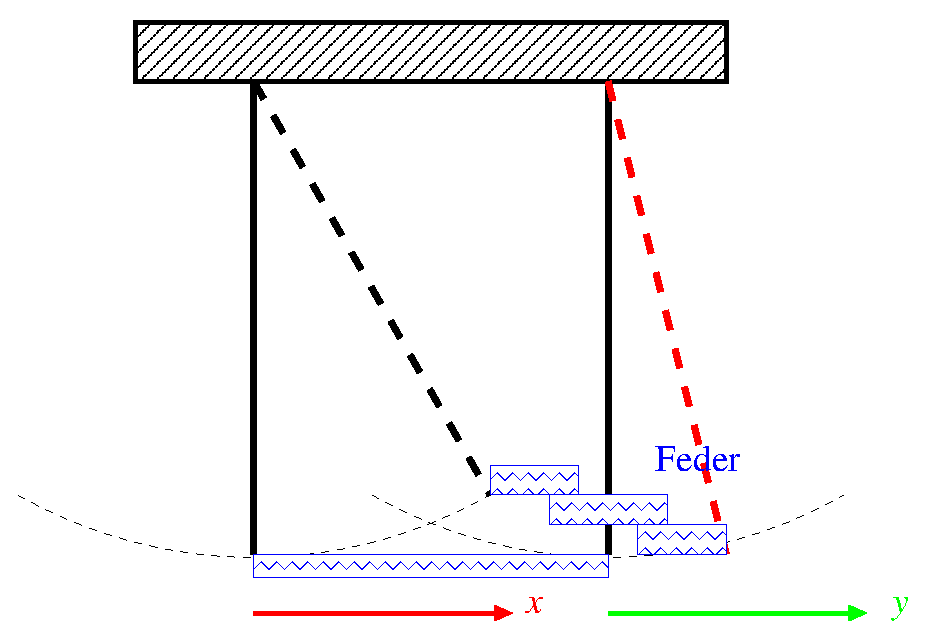
\includegraphics[width=0.5\textwidth]{bilder/gekoppelt}
   \caption[Gekoppeltes Fadenpendel]{Gekoppeltes Fadenpendel (Die
     gestauchte Feder soll die Verk"urzung der Feder als "Uberlappung
     symbolisieren)}
   \label{abb_gekoppelt}
\end{figure}

\begin{Wichtig}
   Aus diesen beiden Schwingungszust"anden kann man jede Bewegung
   gekoppelter Pendel durch "Uberlagerung erzeugen.
\end{Wichtig}
Bspw. ist in Abb. \ref{abb_schwebung} die Schwingung der beiden Pendel
dargestelle, wenn nur eines der beiden zu Anfang der Schwingung
ausgelenkt war. Man nennt diese Verhalten
\textbf{\index{Schwebung}Schwebung}. Hier wechselt die kinetische
Energie st"andig zwischen den beiden Pendeln hin und her.

\begin{figure}
   \centering
   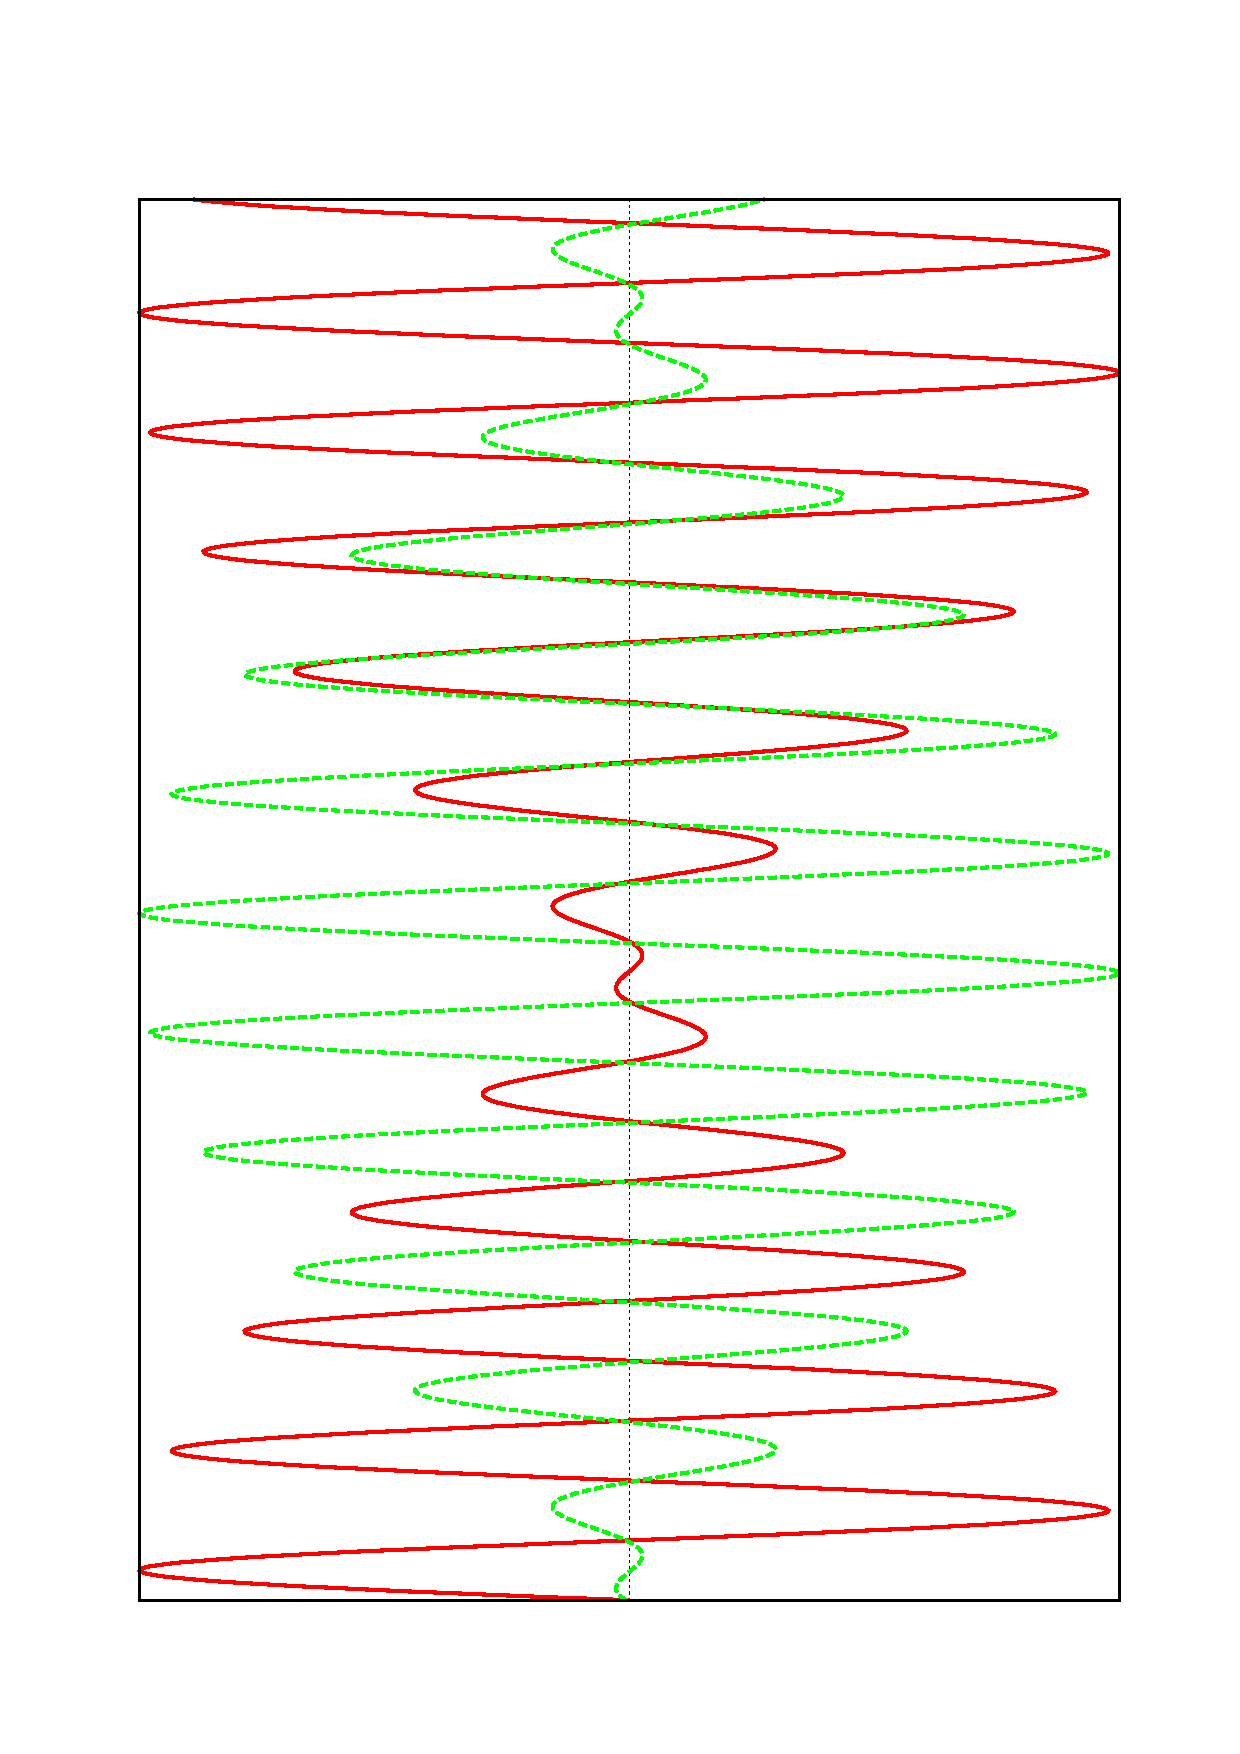
\includegraphics[width=0.7\textwidth,angle=-90]{bilder/schwebung}
   \caption[Schwebung]{Schwebung: Nur eines der beiden gekoppelten
     Pendel ist zu Anfang ausgelenkt}
   \label{abb_schwebung}
\end{figure}




\subsection{Entkoppeln ohne Ansatz}
\label{kap_entkoppeln-ohne-ansatz}

Oben haben wir den Sinusansatz wieder durch \emph{\index{Clever
    guess}Clever guess}
(vgl. Kap. \ref{kap_then-a-wonder-occurs-ansatz}) gefunden. Wir wollen
das Problem nochmal besprechen, wobei wir einen etwas allgemeineren
Ansatz w"ahlen. Wir gehen wieder aus von den Bewegungsgleichungen
\begin{equation}
   \label{eq:24}
   \begin{split}
      m \ddot x + Kx + D(x -y) = 0\\
      m \ddot y + Ky + D(y -x) = 0
   \end{split}
\end{equation}
aus, nur dass wir sie diesmal einmal addieren und einmal
subtrahieren:
\begin{equation}
   \label{eq:25}
   \begin{split}
      m (\ddot x - \ddot y) + K(x - y) + 2D(x - y) = 0 \\
      m (\ddot x + \ddot y) + K(x + y) = 0 
   \end{split}
\end{equation}
Durch "`\index{Koordinatentransformation"'}Koordinatentransformation"'
erh"alt man daraus die zwei neuen Bewegungsgleichungen
\begin{equation}
   \label{eq:26}
   \begin{split}
      m \ddot u + Ku + 2D u = 0 \text{ oder } m \ddot u + (K + 2D)u = 0\\
      m \ddot v + Kv = 0
   \end{split}
\end{equation}
Die wir einfach l"osen k"onnen: Es handelt sich um \emph{harmonische
  Schwingungen}, die wir aus Kap. \ref{kap_freie-schwingung}
kennen. So kennen wir auch die L"osung daf"ur:
\begin{equation}
   \label{eq:27}
   u(t) = \hat u \cdot \cos(\sqrt{\frac{K+2D}{m}} \cdot t + \varphi)
   \text{ und }
v(t) = \hat v \cdot \cos(\sqrt{\frac{K}{m}}\cdot t + \psi)
\end{equation}
Auf die eigentlichen Koordinaten $x$ und $y$ kommen wir nun wieder
durch Addition und Subtraktion von $u$ und $v$:
\begin{equation}
   \label{eq:28}
   x = \frac{1}{2}(v+u) \text{ und } y = \frac{1}{2}(v-u)
\end{equation}
"Uber die Anfangsbedingungen erh"alt man Gr"o"sen f"ur $\hat u$ und $\hat
v$ (und $\varphi$ und $\psi$), die dar"uber bestimmen, welchen Anteil
$u$ und $v$ an $x$ und $y$ haben.






\subsection{Entkoppeln mit Matrix}
\label{kap_entkoppeln-mit-matrix}

Wir stellen nun den Schwinger durch einen \emph{Vektor} dar: $\vec z =
(x,y)^T$. Damit ver"andert sich \eqref{eq:24} zur Vektorgleichung
\begin{equation}
   \label{eq:22}
   m \ddot{\vec z} + 
   \begin{pmatrix}
      K+D & -D\\
      -D & K+D
   \end{pmatrix} \cdot \vec z
= 
\vec 0 ~ \text{ oder } ~ 
   \begin{pmatrix}
      m \frac{\diff ^2}{\diff t^2} + K+D & -D\\
      -D & m \frac{\diff ^2}{\diff t^2} + K+D
   \end{pmatrix} \cdot \vec z = \vec 0
\end{equation}
Als allgemeinen Ansatz machen wir
(vgl. Kap. \ref{kap_allgemeiner-ansatz})
\begin{equation}
   \label{eq:23}
   \vec z = \vec z(t) = \vec Z \cdot \E^{\lambda t}
\end{equation}
Damit erh"alt man
\begin{equation}
   \label{eq:29}
     \begin{pmatrix}
      m \lambda^2 + K+D & -D\\
      -D & m \lambda^2 + K+D
   \end{pmatrix} \cdot \vec z = \vec 0 
~\text{ oder } ~ \Mat A \cdot \vec z = \vec 0
\end{equation}
Damit diese Gleichung nicht trivial wird (also $\vec z = \vec 0$),
muss $\det \Mat A \equiv 0$ werden\footnote{Sonst (also $\det \Mat A
  \neq 0$) sind die Spalten von $\Mat A$ linear unabh"angig und damit
  k"onnen sie nur durch die triviale Linearkombination zu $0$ addiert
  werden.}. F"ur die $2\times 2$-Matrix ist dies noch machbar: 
\begin{equation}
   \label{eq:200}
   \left (m \lambda^2 + K+D \right)^2 - D^2 \equiv 0
\end{equation}
und so erh"alt man f"ur $\lambda$ die Identit"aten:
\begin{equation}
   \label{eq:201}
   \lambda = -\sqrt{-\frac{K}{m}} \text{, } 
\lambda = \sqrt{-\frac{K}{m}}
\text{, }
\lambda =-\sqrt{-\frac{K}{m}-\frac{2\,D}{m}}
\text{, }
\lambda=\sqrt{-\frac{K}{m}-\frac{2\,D}{m}}
\end{equation}
Dabei haben wir stets negative Wurzeln -- also Komplexe Zahlen! Dies
wiederum bedeutet, dass in unserem Ansatz \eqref{eq:23} der $\E$-Term
eine Schwingung beschreibt. Die Korrekte L"osung besteht aus einer
Linearkombination von vier Termen nach \eqref{eq:23} wobei alle $\vec
Z$ -- theoretisch -- frei bestimmbar sind. Weil wir jedoch wieder nur
an \emph{rellen} L"osungen interessiert sind, m"ussen die $\vec Z$
jeweils f"ur die beiden ersten und die beiden Letzten $\lambda$ aus
\eqref{eq:201} voneinander das komplexe Konjugat sein; damit bekommen
wir aber weiterhin \emph{vier} Freiheitsgrade. Wie in
Kap. \ref{kap_allgemeiner-ansatz} bekommen wir zwei (komplexe)
Vektoren $\vec Z$ und zwei \emph{Phasenverschiebungen} der Cosini.

Hier haben wir die ganze Zeit "uber angenommen, dass die beiden Massen
$m$ gleich sind, ebenso wie dass die beiden Federn $K$ gleich hart
sind. Wenn dem \emph{nicht} so w"are, w"are die L"osung mit diesem Ansatz
ebenso zu bestimmen -- nur ein wenig komplizierter. Die Ausdr"ucke (f"ur
\emph{ein} $\lambda$) sind so lange, dass sie nicht in eine Zeile hier
passen...
















\section{"Uberlagerung von Schwingungen -- Interferenz}
\label{kap_uberlagerung-con-schwingungen-interferenz}

\subsection{Gleiche Frequenz}
\label{kap_gleiche-frequenz}

\begin{eqnarray}
\nonumber
   x &=& A \sin (\omega t)\\
\nonumber
   y &=& B \sin (\omega t)\\
   \label{eq:145}
   x+y &=& (A+B) \cdot \sin (\omega t)
\end{eqnarray}

\subsection{Unterschiedliche Frequenz}
\label{kap_unterschiedliche-frequenz}

\begin{eqnarray}
\nonumber
   x &=& A \sin(\omega_1 t)\\
\nonumber
   y &=& A \sin(\omega_2 t)\\
   \label{eq:146}
   x+y &=& 2A \cdot \sin\left ( \frac{\omega_1 + \omega_2}{2} \cdot t \right
   ) \cdot \cos \left ( \frac{\omega_1 - \omega_2}{2}\cdot t \right )
\end{eqnarray}
Wir benutzen dabei ein Additionstheorem f"ur $\sin(\vartheta) +
\sin(\vartheta)$.  Siehe auch
Kap. \ref{kap_phasen-und-gruppengeschwindigkeit-bei-uberlagerung}.



\subsection{Beliebige Schwingungen}
\label{kap_beliebige-schwingungen}

Dank der \textsc{Fourier}-Analyse ist es m"oglich, jede periodische
Funktion aus Sinus- und Cosinus-Schwingungen zusammenzusetzen.

In der Realit"at ist das nicht immer m"oglich, weil bspw. die Federh"arte
nicht konstant ist und so die formal mit Sinusschwingungen gel"osten
Bewegungen eigentlich gar keine solche absolvieren.









\section{Fortschreitende Welle}
\label{kap_fortschreitende-welle}


\begin{Wichtig}
   [\index{Energietransport}\index{Massentransport}Energietransport]
   Bei einer Schwingung wird \emph{Energie} transportiert. Die
   Massenteilchen selbst bleiben am Ort und schwingen nur um eine
   Ruhelage.
\end{Wichtig}


\subsection{Wellengleichung und Definitionen}
\label{kap_wellengleichung-und-definitionen}



Wir gehen von der Schwingung in der Zeit an einem Ort (wir denken sie
uns im Ursprung) mit der Gleichung 
\begin{equation}
   \label{eq:147}
   y_0(t) = \hat y \sin(\omega t + \varphi_0)
\end{equation}
"uber zu einer Schwingung, die zus"atzlich noch eine r"aumliche
Komponente hat.
\begin{Def}
   [\index{Wellenl"ange}Wellenl"ange $\lambda$]
Der r"aumliche Abstand zwischen zwei phasengleich schwingenden Punkten
einer Welle.
\end{Def}
% Die R"aumliche Komponente:

% \begin{equation}
%    \label{eq:148}
%    y(x)
% = \hat y \sin \left (\frac{-2\pi}{\lambda}x \right ) = 
% -\hat y \sin \left (2\pi\frac{x}{\lambda} \right )
% \end{equation}


Die "Uberlegung ist, dass je weiter in $x$-Richtung wir uns von dem in
\eqref{eq:147} betrachteten Schwinger wegbewegen, die Schwingung in
einer anderen Phase ist. Wenn man ein ganzzahliges Vielfaches der
Wellenl"ange zur"uckgelegt hat, soll die Phase wieder die gleiche
sein. Deshalb teilen wir die Entfernung $x$ durch die Wellenl"ange
$\lambda$ und haben so die Entfernung normiert als \emph{Anzahl von
  Wellenl"angen}. Genau so oft hat die Welle bis zum Punkt $x$ schon
eine komplette Periode hinter sich. Eine Periode des Sinus ist $2\pi$
lang -- also hat die Welle bis zum Punkt $x$ die Phasendifferenz
$2\pi\frac{x}{\lambda}$ zum Ursprungspunkt der mit Gl.  \eqref{eq:147}
beschrieben wird. Also hat der Punkt $x$ die Phase
$$
\varphi(x) =
\varphi_0 + 2\pi\frac{x}{\lambda}
$$


Um die Schwingung im Punkt $x$ zur Zeit $t$ zu berechnen, k"onnen wir
die Schwingung im Punkt $x = 0$ betrachten -- also Gl. \eqref{eq:147}
verwenden. % Im Punkt $x$ hat die Schwingung aber eine andere Phase --
% und zwar muss man von der Phase $\omega t + \varphi_0$ die
% Phasendifferenz $2\pi\frac{x}{\lambda}$ abziehen, weil der
% Schwingungszustand, der aktuell in $x = 0$ herrscht, noch
% $2\pi\frac{x}{\lambda}$ \emph{vor} dem aktuellen Zustand liegt.
Indem wir von der Phase der Schwingung im Punkt $x$ den Wert
$\varphi(x)$ abziehen, erhalten wir die Phase, die der Punkt in $x=0$
zur Zeit $t$ hat und k"onnen so $y(x,t)$ ausrechnen.

Es ergibt sich die Wellengleichung
\begin{equation*}
y = y(x,t) = \hat y \cdot \sin \left ( \omega \cdot t - \frac{2\pi}{\lambda}
   \cdot x \right ) 
\end{equation*}
Eine Kleine Erinnerung: Wir k"onnen die Gleichung auch schreiben als
\begin{equation*}
   y = y(x,t) = \hat y \cdot \sin \left ( \frac{2\pi}{T} \cdot t - \frac{2\pi}{\lambda}
   \cdot x \right )
\end{equation*}
Damit sieht man den Zusammenhang von Periodendauer $T$ und Wellenl"ange
$\lambda$ noch besser. Wie man die Frequenz $\omega$ als Abk"urzung
$\omega = \frac{2\pi}{T}$ verwendet, verwendet man als Abk"urzung von $\frac{2\pi}{\lambda}$:
\begin{Def}
   [(\index{Kreiswellenzahl}Kreis)\index{Wellenzahl}\index{Wellenvektor}Wellenzahl
   $k$] mit 
   \begin{equation}
      \label{eq:205}
      k = \frac{2\pi}{\lambda}
   \end{equation}
\end{Def}
Damit k"onnen wir die Gleichung f"ur $y(x,t)$ noch weiter umschreiben:
\begin{equation}
   \label{eqn_welle_1dim}
   \boxed{
y = y(x,t) = \hat y \cdot \sin \left ( \omega \, t - k \, x \right ) }
\end{equation}

\bigskip


\begin{Def}
   [\index{Ausbreitungsgeschwindigkeit}Ausbreitungs- /
   \index{Phasengeschwindigkeit}Phasengeschwindigkeit $c$ oder
   $c_\text{Phase}$] Ein bestimmter Schwingungszustand der Schwingung
   -- also eine gewisse Phase -- bewegt sich mit der Geschwindigkeit
   $c$ fort.
   \begin{equation}
      \label{eqn_def_ausbreitungsgeschw}
      c_\text{Phase} = \frac{\lambda}{T} = \frac{\omega}{2\pi} \lambda = \lambda
      \cdot \nu
=
\frac{\omega}{k}
   \end{equation}
\end{Def}
mit der Kreiswellenzahl $k$ (s. \eqref{eq:205}) und
\begin{Def}
   [\index{Periodendauer}Periodendauer $T$]
An einem Ort dauert es $T$ bis sich der selbe Schwingungszustand
wieder eingestellt hat.
\end{Def}
D.h. die Gleichung 
$$
c = \frac{\lambda}{T}
$$
entspricht 
$$
v = \frac{s}{t}
$$




\subsection{Differenzielle Form der Wellengleichung}
\label{kap_differenzielle-form-wellengleichung}

Im Speziellen Fall f"ur nur eine Dimension gilt:
\begin{equation}
   \label{eq:149}
   \frac{\partial^2}{\partial t^2} y = c^2 \cdot
   \frac{\partial^2}{\partial x^2} y
\end{equation}
Der Allgemeine Fall ber"ucksichtigt noch mehr Raumdimensionen $x_i$:
\begin{equation}
   \label{eq:150}
   \frac{1}{c^2} \frac{\partial^2 }{\partial t^2} \vec y - \sum_{i=1}^n
   \left ( \frac{\partial ^2}{\partial x_i^2} \vec y \right ) = 0
\end{equation}
Dabei k"onnen wir dies mit dem \textsc{Laplace}-Operator $\Delta$
umschreiben zu:
\begin{equation}
   \label{eqn_wellengleichung}
\boxed{
  \frac{1}{c^2} \frac{\partial^2 }{\partial t^2} \vec y - \Delta
  \vec y = 0 
}
\end{equation}

Wenn wir nun unsere Gleichung \eqref{eqn_welle_1dim} einsetzen,
so erhalten wir:
\begin{equation}
   \label{eq:151}
   \frac{\omega^2}{c^2} = \frac{4\pi^2}{\lambda^2}
\end{equation}
und damit wieder den Zusammenhang aus
\eqref{eqn_def_ausbreitungsgeschw}. Die von uns anschaulich
hergeleitete L"osung stimmt also.









\section{Arten von Wellen}
\label{kap_arten-von-wellen-1}

Wir unterscheiden zwei Typen:
\begin{description}[\setlabelstyle{\bfseries\slshape}]
\item[\index{Transversalwellen}Transversalwellen]  Schwingen \emph{senkrecht} zu ihrer
   Ausbreitungsgeschwindigkeit (bspw. Wasserwellen)
\item[\index{Longitudialwellen}Longitudialwellen] Schwingen \emph{parallel} zur
   Ausbreitungsrichtung (bspw. Schallwellen\footnote{Der Mensch kann
     Schallwellen mit Frequenzen von $\nu \in [20\operatorname{Hz};
     20\, 000 \operatorname{Hz}]$ wahrnehmen.})
\end{description}




\section{Interferenz}
\label{kap_interferenz}



Zwei Wellen durchdringen sich im Allgemeinen ohne Probleme -- also
gehen \emph{unver"andert} weiter. In dem Bereich, in dem sie sich
durchdringen \textbf{"uberlagern} sie sich; ihre Auslenkungen addieren
sich.

Im besonderen Fall hat man zwei Wellen der selben Frequenz $\nu$; hier
ergeben sich zwei Spezialf"alle:
\begin{Def}[konstruktive und destruktive Interferenz]
   Bei \textbf{\index{konstruktive Interferenz}konstruktiver
     Interferenz} hat die Summe der Wellen eine maximale Amplitude
   ($|\hat y_1| +| \hat y_2|$), bei \textbf{\index{destruktive
       Interferenz}destruktiver Interferenz} wird die Amplitude der
   "Uberlagerung minimal ($||\hat y_1| - |\hat y_2||$).
\end{Def}
Haben die Wellen sogar die gleiche Amplitude $\hat y$, so hat die
"Uberlagerung bei konstruktiver Interferenz die Amplitude $2 \hat y$
und bei destruktiver Interferenz verschwindet die Amplitude der
"Uberlagerung.

Wir definieren
\begin{Def}
   [\index{Gangunterschied}Gangunterschied $\Delta s$]
Der k"urzeste r"aumliche Abstand zwischen zwei gleichen
Schwingungszust"anden zwischen zwei verschiedenen ("uberlagernden) Wellen.
\end{Def}
und analog dazu
\begin{Def}
   [\index{Phasendifferenz}Phasendifferenz $\Delta \varphi$]
Der Unterschied der Phasen zweier Wellen am selben Ort.
\end{Def}
Es gilt der Zusammenhang
\begin{equation}
   \label{eq:152}
   \Delta \varphi = \frac{2\pi}{\lambda} \cdot \Delta s \text{ ~ oder
   } \frac{\Delta \varphi}{\Delta s} = k
\end{equation}
wobei $k$ die \emph{Kreiswellenzahl} aus \eqref{eq:205} ist.

Wir betrachten gleichf"ormige (also gleiche Frequenz
bzw. Wellenl"ange und Amplitude) Wellen $x$, $y$ und $z$:
\begin{equation*}
   x = A \cos(\omega t - kx) \text{, } y = A \cos(\omega t  - k
   (x+\Delta s))
\text{ und } z = A \cos(\omega t - kx + \Delta \varphi)
\end{equation*}
Anschaulich ist klar, dass sich genau dann eine maximale Amplitude von
$2A$ ergibt, wenn die Argumente der Cosini sich um vielfache von
$2\pi$ unterscheiden und genau dann die minimale Amplitude von $A-A =
0$, wenn sich die Argumente um $\pi, 3\pi, 5\pi,...$
unterscheiden. F"ur die \emph{Phasendifferenz} $\Delta \varphi$ kann man so
sofort die gew"unschten Bedingungen finden (s. \eqref{eq:202} und
\eqref{eq:203}). F"ur den \emph{Gangunterschied} dagegen vergleichen
wir $x$ mit $y$ und sehen, dass $k \Delta s$ f"ur konstruktive
Differenz vielfache von $2\pi$ sein m"ussen und f"ur destruktive
Interferenz $\pi, 3\pi, 5\pi,...$. Dies h"atte man auch aus
Gl. \eqref{eq:152} schlie"sen k"onnen. Es folgen damit die Bedingungen:

\begin{Wichtig}
   [Bedingung: \index{Konstruktive Inverferenz}Konstruktive
   \index{Interferenz!Konstruktive}Interferenz] liegt vor, wenn
\begin{eqnarray}
   \label{eq:155}
   \Delta s &=& \lambda \cdot n ~ ~ ~ n \in \mathbb Z\\
\label{eq:202}
   \Delta\varphi &=& 2\pi \cdot n~ ~ ~ n \in \mathbb Z
\end{eqnarray}
\end{Wichtig}

und

\begin{Wichtig}
   [Bedingung: \index{Destruktive Interferenz}Destruktive
   \index{Interferenz!Destruktive}Interferenz] liegt vor, wenn
\begin{eqnarray}
\label{eq:157}
   \Delta s &=& n \cdot \lambda + \frac{\lambda }{2} ~ ~ ~ n \in
   \mathbb Z\\
\label{eq:203}
   \Delta\varphi &=& n \cdot 2\pi  + \pi~ ~ ~ n \in \mathbb Z
\end{eqnarray}
\end{Wichtig}




\section{Phasen- und Gruppengeschwindigkeit bei "Uberlagerung}
\label{kap_phasen-und-gruppengeschwindigkeit-bei-uberlagerung}

Wir wollen zwei Wellen mit verschiedenen Wellenl"angen und Frequenzen
"uberlagern. Mit der Kreiswellenzahl $K_i = \frac{2\pi}{\lambda_i}$ 
gilt
\begin{eqnarray}
   \label{eq:164}
   u = A \sin (\omega_1 t - K_1 x)\\
   v = A \sin(\omega_2 t - K_2 x)
\end{eqnarray}
und mit  dem
Additionstheorem
$$
\sin \alpha + \sin \beta = 2 \sin \frac{\alpha + \beta}{2} \cos
\frac{\alpha - \beta}{2}
$$
weiter:
\begin{equation}
   \label{eq:165}
\boxed{ u + v = 
 2 A \cdot \sin \left ( \underbrace{\frac{\omega_1 + \omega_2}{2}}_\omega t - \underbrace{ \frac{K_1 +
     K_2}{2}}_K x \right ) \cdot \cos \left ( \frac{\omega_1 -
     \omega_2}{2}t - \frac{K_1  - K_2}{2}x \right )
}
\end{equation}
und damit
\begin{equation}
   \label{eq:166}
   u+v = 2A \cdot \sin (\omega t - K x) \cdot \cos \left ( \frac{1}{2} (\Delta \omega \cdot t -
   \Delta K \cdot x ) \right )
\end{equation}

Dabei ist der Cosinus-Term die \textbf{\index{Einh"ullende}Einh"ullende} der Schwingung,
weil die Maxima der Schwingung auf ihr liegen. Vgl. dazu
Abb. \ref{abb_einhuell}.

Nun wollen wir die Geschwindigkeit bestimmen, mit der sich die
Einh"ullende fortbewegt. Dazu betrachten wir ein Maximum der
Einh"ullenden; dazu muss $\cos = 1$ sein, also am besten:
\begin{equation}
   \label{eq:168}
   \left ( \frac{1}{2} (\Delta \omega \cdot t -
   \Delta K \cdot x ) \right ) = 0
\end{equation}
Wenn wir diese Gleichung mit $\frac{1}{2}$ k"urzen und nach
$\frac{x}{t} = v$ aufl"osen, bekommen wir genau
Gl. \eqref{eqn_gruppengeschwindigkeit}.\footnote{Dabei haben wir die
  Annahme gemacht, dass die Gruppengeschwindigkeit \emph{linear}, also
nicht beschleunigt ist. Diese Behauptund d"urfen wir machen, weil die
Wellen $u$ und $v$ selbst auch nicht beschleunigt waren, sondern sich
linear mit $c_\text{Phase}$ ausgebreitet haben.}


Wir definieren:
\begin{Def}[Gruppengeschwindigkeit $c_\text{Gruppe}$]
   Die Geschwindigkeit, mit der sich ein Schwingungszustand der
   Einh"ullenden bewegt ist die
   \textbf{\index{Gruppengeschwindigkeit}Gruppengeschwindigkeit}.
   \begin{equation}
      \label{eqn_gruppengeschwindigkeit}
      c_\text{Gruppe} = \frac{\Delta \omega}{\Delta K}
   \end{equation}
\end{Def}


\begin{figure}
   \centering
   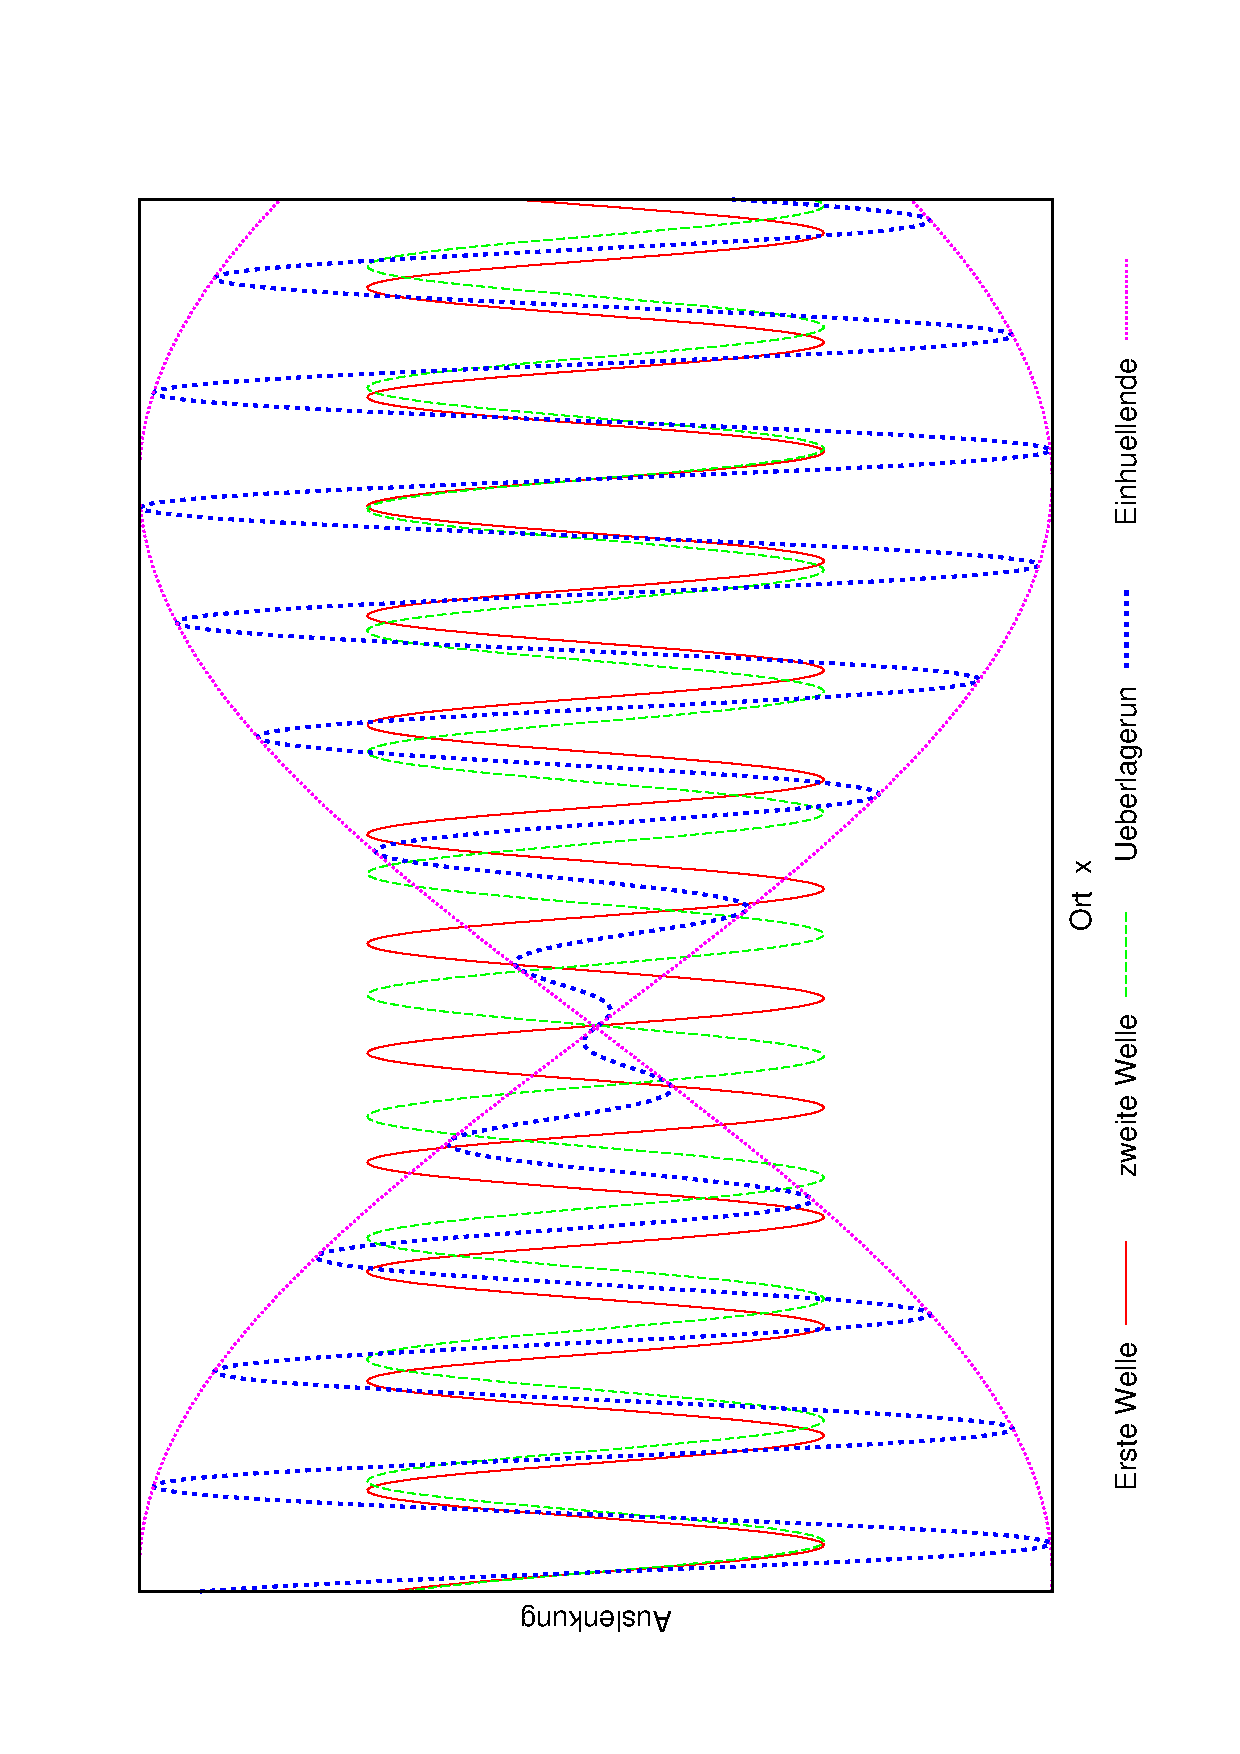
\includegraphics[width=0.7\textwidth,angle=-90]{bilder/einhuell}
   \caption[Überlappung zweier Wellen]{Zwei Wellen, deren
     "Uberlagerung und die Einh"ullende}
   \label{abb_einhuell}
\end{figure}

\bigskip
Als \textbf{Zusammenhang zwischen $c_\text{Gruppe}$ und
  $c_\text{Phase}$} finden wir, das bei einer infinitissimalen
Betrachtung von Gl. \eqref{eqn_gruppengeschwindigkeit}, wobei wir
$\omega$ durch $\omega = c_\text{Phase} \cdot K$ ersetzen:
\begin{equation}
   \label{eq:167}
   c_\text{Gruppe} = \frac{\diff \omega}{\diff K} = \frac{\diff
     (c_\text{Phase} \cdot K)}{\diff K} = c_\text{Phase}\frac{\diff K}{\diff K}
   + K \frac{\diff c_\text{Phase}}{\diff K}
\end{equation}
Wobei $\frac{\diff K}{\diff K} = 1$ ist. Wenn wir $K =
\frac{2\pi}{\lambda}$  einsetzen, erhalten wir so (weil $\diff K =
\diff \frac{2\pi}{\lambda} = - 2\pi \cdot \frac{1}{\lambda^2} \diff
\lambda$):
\begin{equation}
   \label{eq:169}
   c_\text{Gruppe} = c_\text{Phase} - K \frac{\lambda^2}{2\pi}
   \frac{\diff c_\text{Phase}}{\diff \lambda} 
=
\boxed{ c_\text{Phase} - \lambda \cdot \frac{\diff c_\text{Phase}}{\diff
  \lambda} = c_\text{Gruppe} }
\end{equation}




\section{Reflexion}
\label{kap_reflexion}

Wenn Wellen an einem \textbf{\index{festes Ende}festen Ende} auf ein
Hindernis treffen, so k"onnen die Enden des Wellentr"agers nicht
schwingen und damit keine Schwingungsenergie aufnehmen: Die Energie
der Welle wird wieder zur"uck auf die Welle geworfen.

Man kann sich vorstelle, dass die Welle die Wand mit Kraft $F$ bewegen
will (es aber nicht schafft) daf"ur die Wand die Welle aber mit der
Reactio $F$ in die Gegenrichtung zur"uckbewegt. 

Direkt an der Wand liegt ein \textbf{\index{Phasensprung}Phasensprung} von 
$$
\Delta \varphi = \pi
$$
vor, weil hier die Welle vom unteren Umkehrpunkt unvermittelt zum
bberen Umkehrpunkt "`springt"'.


\bigskip

Wenn der Wellentr"ager mit einem \textbf{\index{loses Ende}losen Ende} zuende geht, so
k"onnen die letzten Teilchen auf dem Wellentr"ager ungehindert
\emph{Schwingungen} ausf"uhren -- sie schwingen also "uber ihre Ruhelage
hinaus und wieder zur"uck und sorgen so daf"ur, dass wenn eine Welle mit
einer \textbf{\index{Schnelle}Schnelle}\footnote{die Bewegung der Schwingung
selbst --
also bei einer Transversalwelle die Geschwindigkeit, mit der ein
Massenteilchen sich senkrecht zur Ausbreitungsrichtung bewegt} nach
nach oben ankommt, nach der Reflexion wieder eine Schnelle nach oben
vorliegt. 

Hier liegt also kein Phasensprung vor:
\begin{equation}
   \label{eq:156}
   \Delta \varphi = 0
\end{equation}









\section{Stehende Wellen}
\label{kap_stehende-wellen}

\subsection{Entstehung und Aussehen}
\label{kap_entstehung-und-aussehen}



Wir betrachten zwei Wellen der gleichen Frequenz und Amplitude, die
aufeinander zulaufen. Ihre Wellengleichungen sind gegeben durch:
\begin{eqnarray*}
   u &=& A \sin \left (\omega t - \frac{2\pi}{\lambda}x \right )\\
   v &=& A \sin \left (\omega t + \frac{2\pi}{\lambda} x\right )
\end{eqnarray*}
Wenn wir diese Wellengleichungen addieren, um die "Uberlagerung zu
erhalten, k"onnen wir $A$ ausklammern und ein Additionstheorem des
Sinus anwenden und erhalten dann
\begin{equation}
   \label{eq:158}
   y = 2A \cos\left ( \frac{2\pi}{\lambda}x \right ) \cdot \sin \left
      ( \omega t \right )
\end{equation}
Wenn wir diese Welle zu verschiedenen Zeiten betrachten
(vgl. Abb. \ref{abb_stehend}), so f"allt auf, dass die $x$-Achse stets
an den selben Punkte geschnitten wird -- diese nennen wir
\textbf{Knoten} -- und dass es Stellen gibt, die sich maximal bewegen
-- \textbf{B"auche}. Wichtig ist dabei, dass weder Knoten noch B"auche
ihre $x$-Position ver"andern. Die Welle \emph{steht} also wirklich auf
einem Fleck und die einzelnen Massenpunkte f"uhren einfache harmonische
Schwingungen aus, wobei entscheidend ist \emph{wo} sie schwingen. Die
Teilchen, die direkt auf einem Knoten liegen, schwingen garnicht,
w"ahrend die Teilchen, die auf einem Bauch liegen, maximal schwingen.

Die Knoten treten in festen Abst"anden auf: An einem Ort ist der
Cosinusterm aus \eqref{eq:158} konstant. Wenn er also verschwindet,
verschwindet auch die Schwingung an dieser Stelle und wir haben einen
Knoten. Wenn der Cosinusterm dagegen maximal (also 1) wird, haben wir
einen Bauch. Die Knoten liegen also bei
\begin{equation}
   \label{eq:159}
x = \lambda \cdot \frac{2n+1}{4}
\end{equation}
mit $n \in \mathbb Z$ und die B"auche bei
\begin{equation}
   \label{eq:160}
   x = \lambda \cdot \frac{2n}{4}
\end{equation}
% F"ur die Amplitude $\hat y$ an einen Punkt, der von einem Bauch den
% Abstand $\delta$ hat, gilt, wenn $2A$ die maximale Amplitude der
% stehenden Welle ist (wenn $A$ die Amplitude einer einzelnen Welle
% war):
% \begin{equation}
%    \label{eq:161}
%    \hat y(\delta) = \pm 2A \cdot \sin \frac{4\delta}{\lambda}
% \end{equation}

\begin{figure}
   \centering
   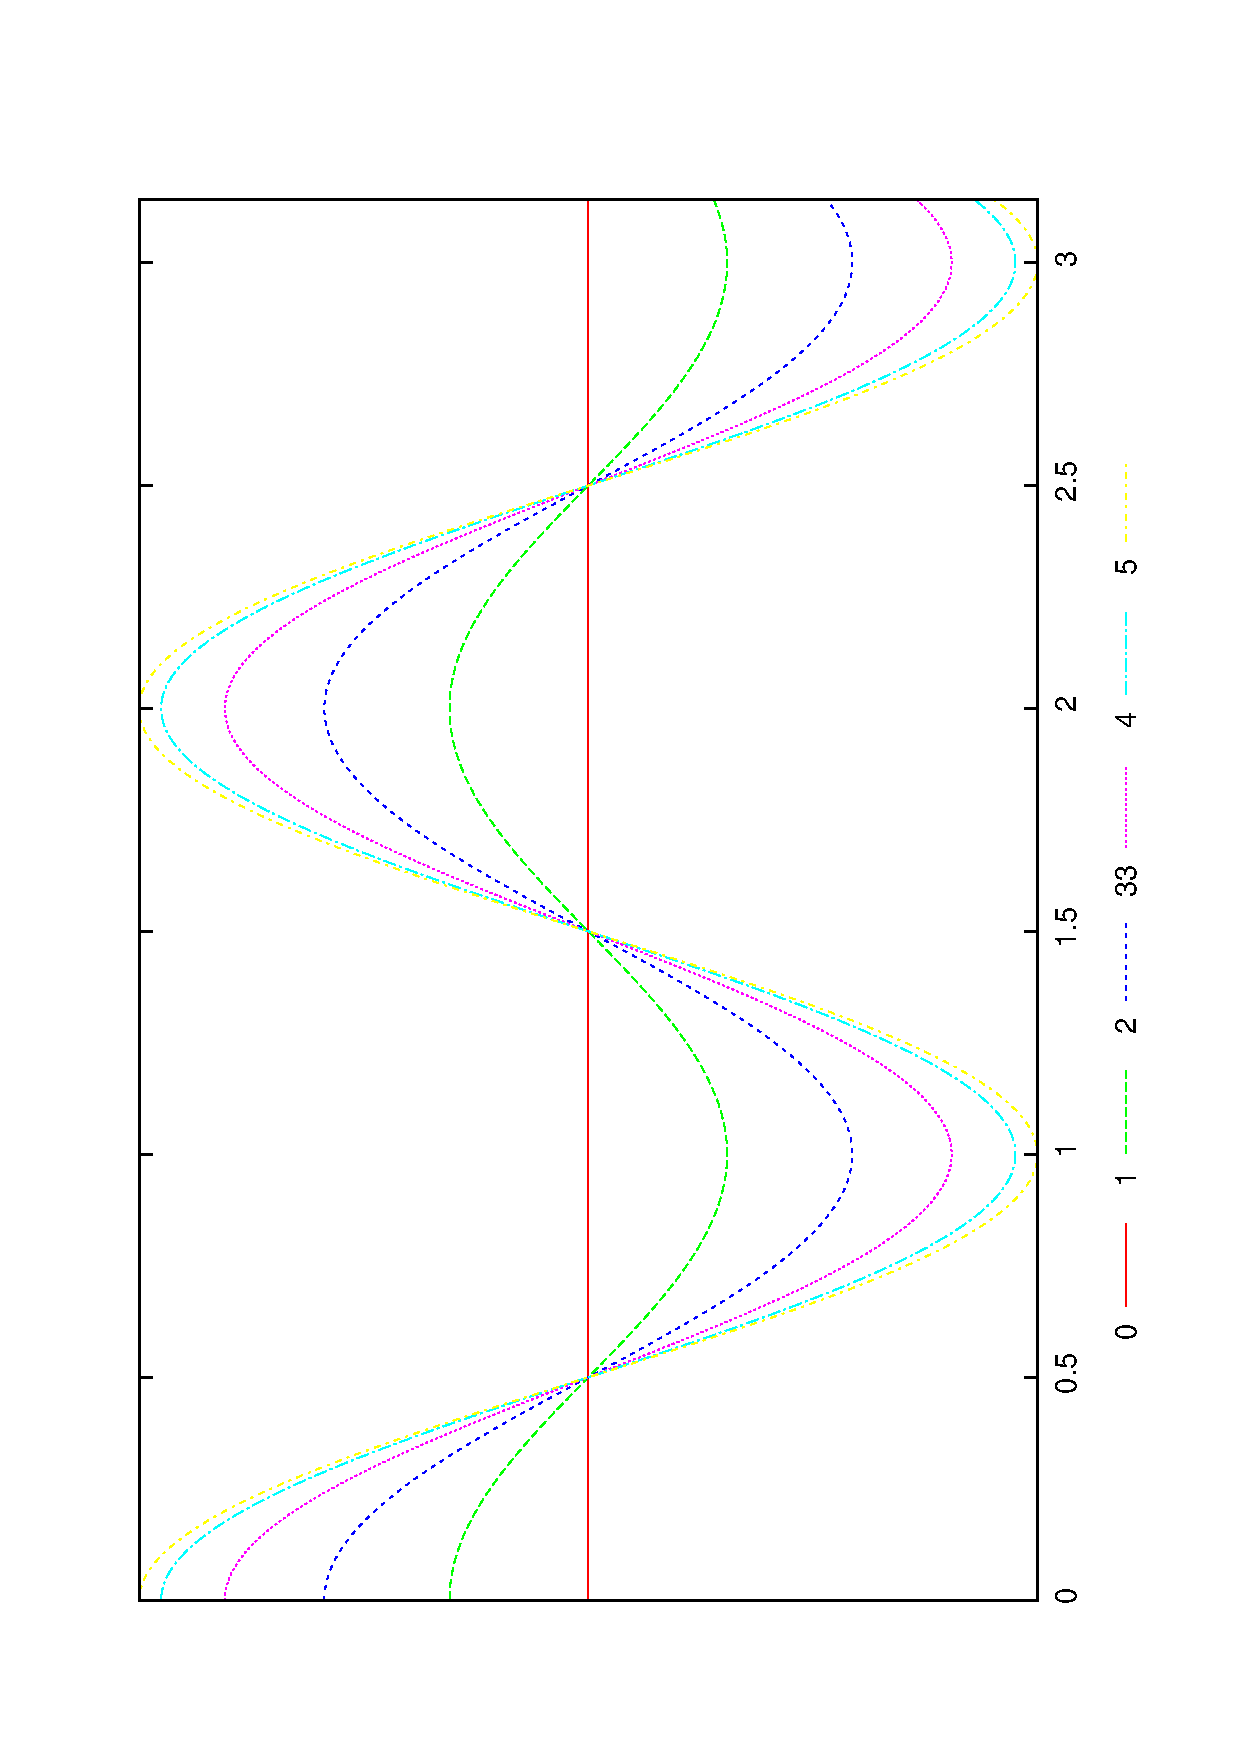
\includegraphics[width=0.7\textwidth,angle=-90]{bilder/stehend}
   \caption{Stehende Welle in 5+1 Zeitschritten}
   \label{abb_stehend}
\end{figure}




\subsection{Visualisierung}
\label{kap_visualisierung}


Wenn nun die schwingenden Teilchen so klein sind, dass wir sie nicht
mehr sehen k"onnen -- also wenn bspw. Luft als Longitudialwelle
schwingt -- dann m"ussen wir uns einen Trick einfallen lassen, um die
Schwingung trotzdem zu visualisieren.

Wenn Luftteilchen Schwingen, so bilden sich Knoten und B"auche der
Luftteilchen; diese werden als \emph{Geschwindigkeits}knoten und
-b"auche bezeichnet. Daneben gibt es noch \emph{Druck}b"auche und
-knoten. Dort wo ein Geschwindigkeitsknoten ist, sitzt ein Druckbauch,
einfach weil hier von links und von rechts st"andig Teilchen an das
ruhende Teilchen sto"sen und dr"ucken und so eine Kraft auf das Teilchen
aus"uben, die wir als Druck interpretieren.

Wir k"onnen nun die Bewegungsknoten visualisieren, indem wir bspw. in
einer R"ohre eine stehende Welle erzeugen, indem wir an beide Enden
Lautsprecher setzen, die den selben Ton spielen. Wenn wir nun kleine
Kr"umel -- bspw. B"arlappsporen, die besonders leicht und fein sind --
gleichm"a"síg im Rohr verteilen, so werden diese an den Stellen
"`weggewischt"', an denen die Geschwindigkeitsb"auche sind und in Ruhe
gelassen, wo die Geschwindigkeitsknoten liegen.  Wir bekommen also
kleine H"aufchen des Staubs bei den Geschwindigkeitsknoten.




\subsection{Auf beschr"anktem Wellentr"ager}
\label{kap_auf-beschranktem-wellentrager}

Nur die wenigsten Wellentr"ager die wir kennen sind unendlich
ausgedehnt. Die L"ange $L$ eines solchen Wellentr"agers bestimmt mit,
was f"ur stehende Wellen sich darauf bilden k"onnen.
\begin{Wichtig}
   Es bilden sich nur stehende Wellen bei characteristischen
   Frequenzen.
\end{Wichtig}
\begin{Def}[Eigenfrequenz $\omega_0$]
   Diese Frequenzen nennen wir
   \textbf{\index{Eigenfrequenz}Eigenfrequenz} des Wellentr"agers.
\end{Def}
Das liegt daran, dass die Enden des Wellentr"agers die Welle
reflektieren -- abh"angig davon, ob wir ein loses oder ein festes Ende
haben mit oder ohne Phasensprung
(s. Kap. \ref{kap_reflexion}). D.h. die Enden des Wellentr"agers sind
entweder selbst (Geschwindigkeits)B"auche (beim losen Ende) oder
(Geschwindigkeits)Knoten (bei festem Ende).

\begin{description}[\setlabelstyle{\bfseries\slshape}]
\item[Zwei feste Enden] Zwei Knoten haben stets den Abstand
   $\frac{\lambda}{2}$. Hat ein Wellentr"ager die L"ange $L$, so kann
   man genau $n$ B"auche darauf platzieren; damit die Knoten mit den
   R"andern zusammenfallen, muss $\frac{\lambda}{2}\, n = L$ sein oder:
%  Damit m"ussen den Abstand $L$ oder
%    $\frac{L}{2}$ oder $\frac{L}{n}$ haben ($n \in \mathbb N$) damit
%    Knoten und Enden des Wellentr"agers zusammenfallen. Da zwei Knoten
%    den Abstand $\frac{\lambda}{2}$ haben, gilt
   \begin{equation}
      \label{eq:153}
      \lambda_n^{(f,f)} = \frac{2\cdot L}{n} ~  ~ \text{ mit } n \in
      \mathbb N
   \end{equation}
Und mit der Ausbreitungsgeschwindigkeit $c$ und
\eqref{eqn_def_ausbreitungsgeschw} gilt f"ur die Frequenz:
\begin{equation}
   \label{eq:154}
   \nu_n^{(f,f)} = \frac{c}{2\cdot L} \cdot n
\end{equation}


\item[Ein festes und ein loses Ende] Zwei Knoten haben weiterhin den
   Abstand $\frac{\lambda}{2}$, aber diesmal kommt an einem Ende noch
   ein Abstand Knoten-Bauch, also $\frac{\lambda}{4}$, dazu.  Wir
   k"onnen auf dem Wellentr"ager also $n$ B"auche zwischen zwei Knoten
   und einen Bauch am losen Ende platzieren. Damit dies mit der L"ange
   "ubereinstimmt, muss $\frac{\lambda}{2}n + \frac{\lambda}{4} = L$
   gelten, oder\footnote{Das "`$-$"' im Nenner kommt daher, dass in
     dieser Gleichung $n\in \mathbb N$ sein soll! Damit man die
     l"angste Schwingung (also maximal gro"ses $\lambda$) damit
     darstellen kann, die einen Bauch und einen Knoten direkt an den
     Enden hat, braucht man im Nenner die $\frac{1}{2}$, und diese
     kann man nur erreichen, wenn man von $1$ die $\frac{1}{2}$
     \emph{abzieht}.}
   \begin{equation}
      \label{eq:162}
      \lambda_n^{(f,l)} = \frac{2 \cdot L}{n - \frac{1}{2}} ~  ~
      \text{ mit } n
      \in \mathbb N
   \end{equation}
und f"ur die Freqnenz:
\begin{equation}
   \label{eq:163}
   \nu_n^{(f,l)} = \frac{c}{2L} \cdot (n - \frac{1}{2} )
\end{equation}
\end{description}



\bigskip

\begin{Def}[Grund- und Oberschwingungen]
   Wir nennen die Schwingung mit der gr"o"st m"oglichen Wellenl"ange (also
   f"ur $n = 1$) \textbf{\index{Grundschwingung}Grundschwingung} und
   jede weitere Schwingung mit entsprechend k"urzerer Wellenl"ange
   $n$-te \textbf{\index{Oberschwingung}Oberschwingung}.
\end{Def}

Bei einem Musikinstrument haben die verschiedenen Oberschwingungen
verschiedene Amplituden. Das Verh"altnis dieser Amplituden zueinander
bestimmt die \textbf{\index{Klangfarbe}Klangfarbe} des Instruments.






\subsection{Funktionsprinzip von Fl"oten}
\label{kap_funktionsprinzip-von-floten}


Durch Lufteinblasen wird ein Blatt (eine Schneide) in Schwingungen
versetzt. Sie regt die Lufts"aule "uber sich in der Fl"ote zu
Schwingungen an (vgl. Abb. \ref{abb_floete}). Je n"aher die Luft am
Blatt ist, desto weniger Bewegungsfreiheit hat sie und schwingt hier
deshalb nur wenig, daf"ur aber entfernt vom Blatt st"arker.  In der N"ahe
des Blattes ist also der Druck gro"s, die Teilchenbewegung klein,
weiter entfernt anders herum.

Die schwingende Lufts"aule kann nun am Ende der Pfeife die Luft der
Umgebung zu Schwingungen anregen -- der Ton wird
"ubertragen. Gleichzeitig wird aber die Schwingung innerhalb der
Pfeife reflektiert und es bildet sich eine stehende Welle aus, wodurch
der Ton sich verst"arken kann (Durch \emph{\index{Resonanz}Resonanz}
kann sich die Amplitude "`aufschaukeln"').  Die \emph{H"ohe} des Tones
h"angt davon ab, wie gut das Blatt schwingen kann buzw. wie
gleichm"a"sig es angeregt wird und von der L"ange der Pfeife.

Wir unterscheiden zwischen \textbf{\index{gedeckte Pfeife}gedeckten}
Pfeifen, die ein Offenes und ein geschlossenes Ende haben und
\textbf{\index{offene Pfeife}offenen} Pfeifen, bei denen beide Enden
offen sind.

In einer Pfeife k"onnen verschiedene Frequenzen stehende Wellen
erzeugen, so lange die Bedingungen aus
Kap. \ref{kap_auf-beschranktem-wellentrager} eingehalten
werden. Vgl. dazu Abb. \ref{abb_pfeifen_schwingung}.


\begin{figure}
   \centering
   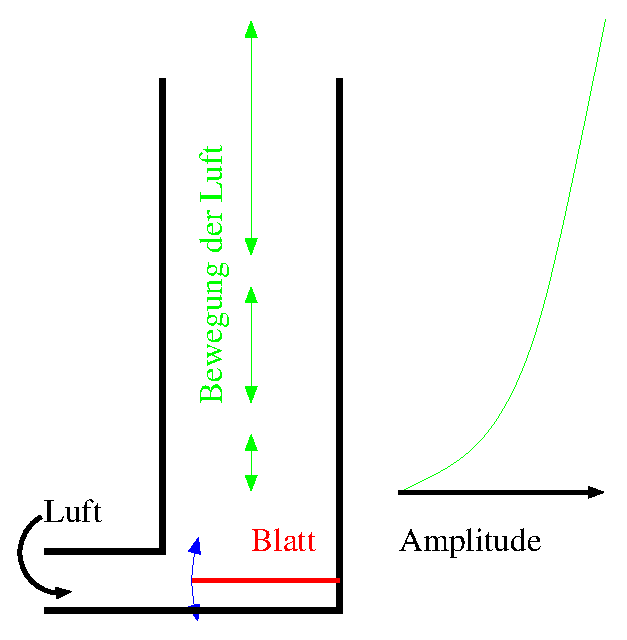
\includegraphics[width=0.5\textwidth]{bilder/floete}
   \caption{Prinzip einer Fl"ote}
   \label{abb_floete}
\end{figure}

\begin{figure}
   \centering
   \subfigure[Gedeckte Pfeife: Links geschlossenes, rechts offenes Ende]{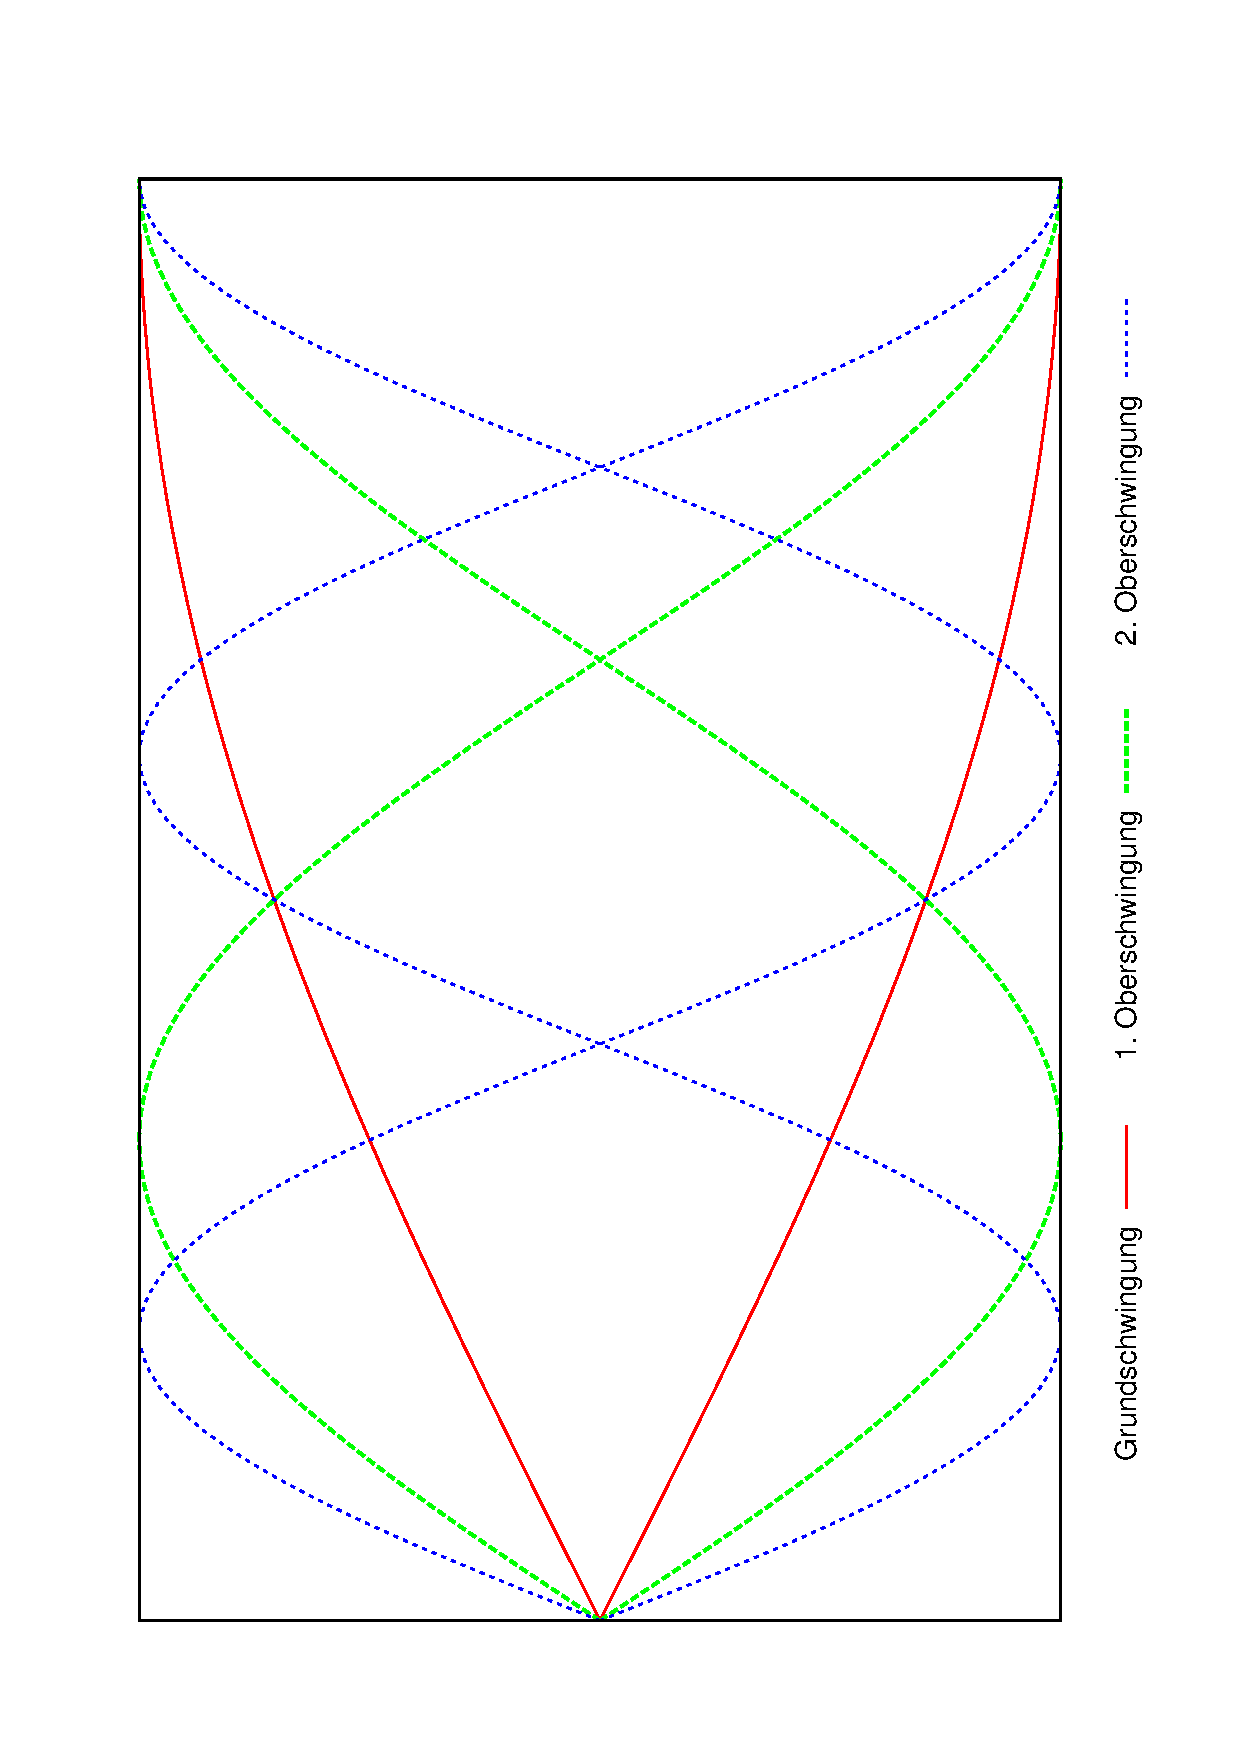
\includegraphics[width=0.3\textwidth,angle=-90]{bilder/gedeckt}}
   \subfigure[Offene Pfeife: Beide Enden offen]{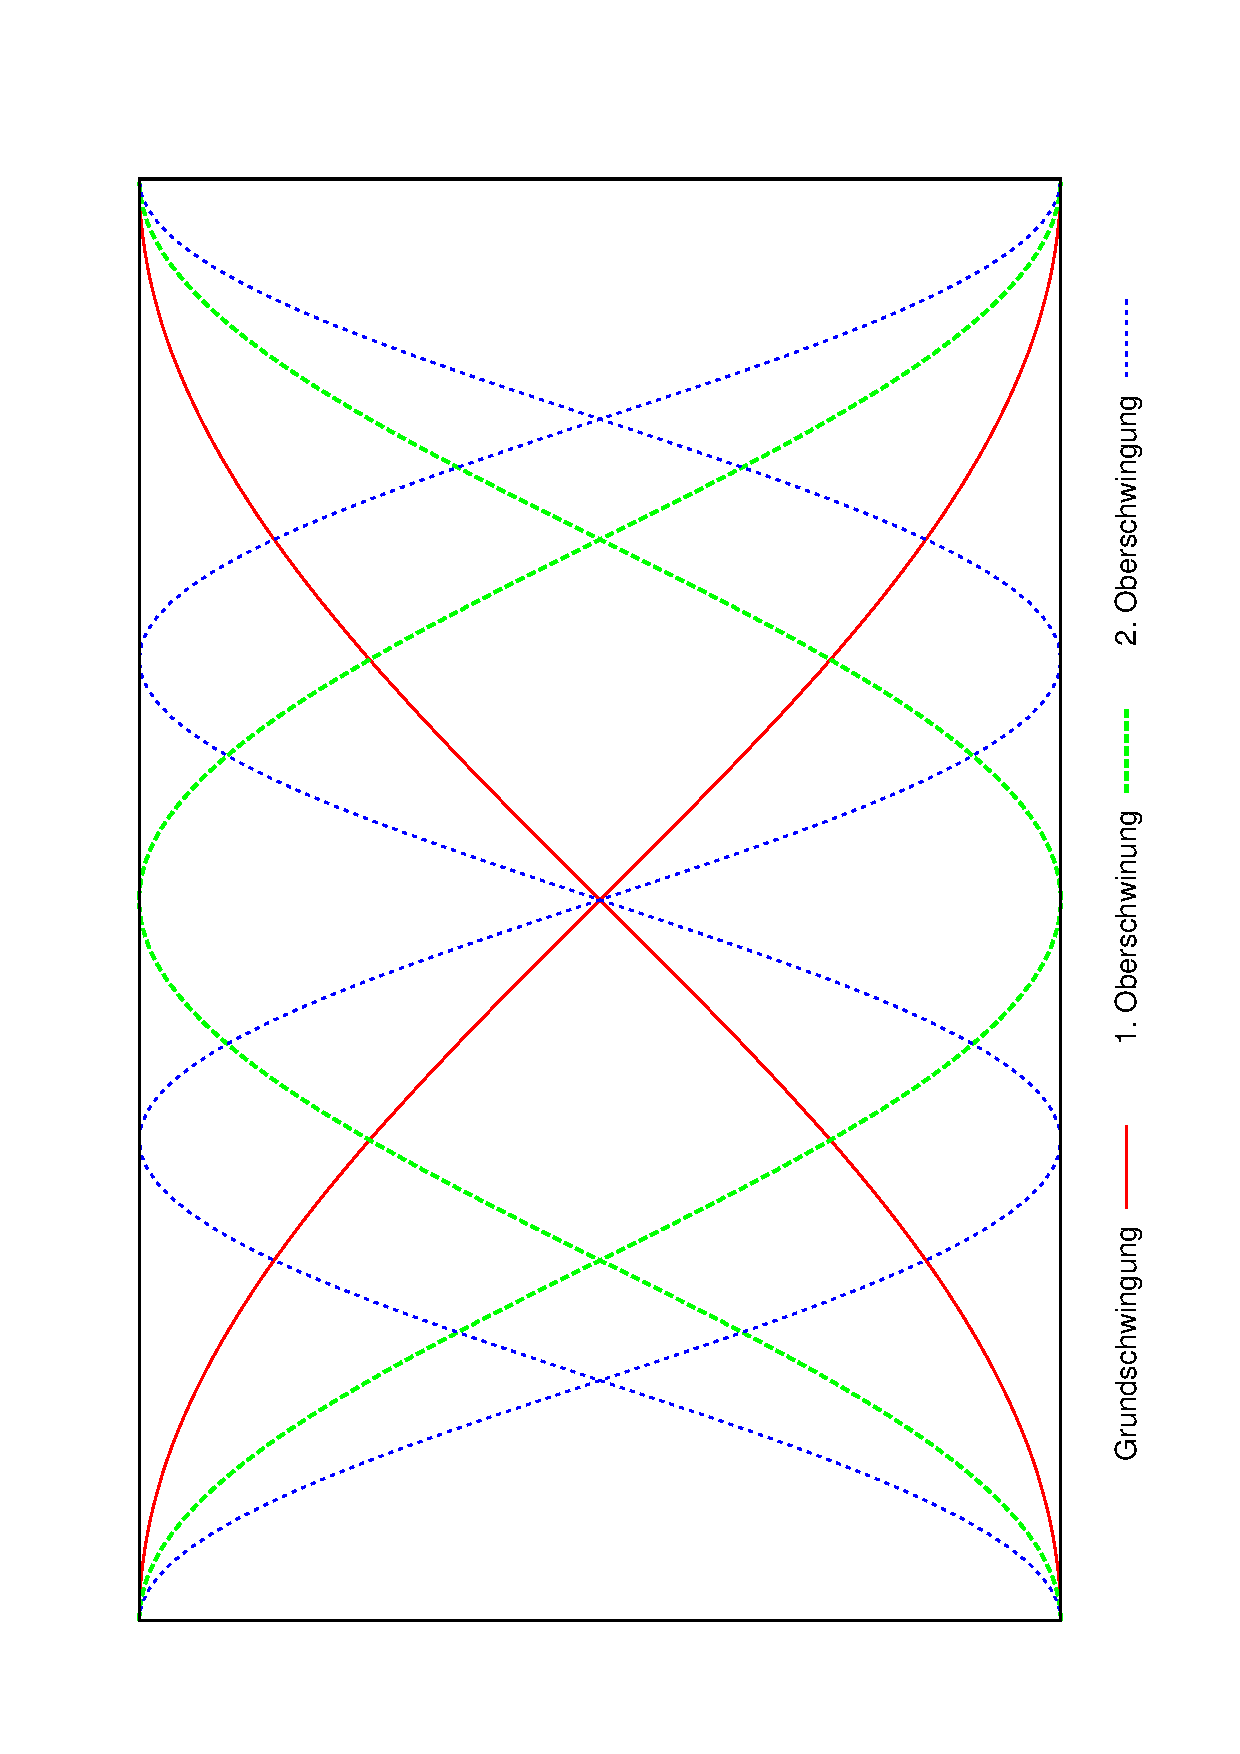
\includegraphics[width=0.3\textwidth,angle=-90]{bilder/offen}}
   \caption{Gedeckte und offene Pfeifen}
   \label{abb_pfeifen_schwingung}
\end{figure}









































%%%%%%%%%%%%%%%%%%%%%%%%%%%%%%%%%%%%%%%%%%%%%%%%%%%%%%%%%%%%%%%%%%

%%%%%%%%%%%%%%%%%%%%%%%%%%%%%%%%%%%%%%%%%%%%%%%%%%%%%%%%%%%%%%%%%

%%%%%%%%%%%%%%%%%%%%%%%%%%%%%%%%%%%%%%%%%%%%%%%%%%%%%%%%%%%%%%%%%



 \chapter{Thermodynamik}
\label{kap_thermodynamik}


In der Thermodynamik betrachten wir keine kleinste schwingende
Teilchen in der Materie sondern schauen uns die makroskopischen
Eigenschaften -- die \textbf{Zustandsgr"o"sen} (wie Temperatur, Entropie
usw) -- an. 

\paragraph{Absolute Temperatur}
\label{kap_absolute-temperatur}

Wir verwenden eine Temperaturskala, deren absoluter Nullpunkt eine
Naturkonstante ist: Je weiter man ein Gas abk"uhlt, desto geringer ist
sein Dampfdruck. Dabei zeigt sich, dass bei der Temperatur
$\mathbf{-273,15^\circ C}$ \emph{alle Gase den Druck $0$ (Pascal)
haben}.






\section{Zustandsgr"o"sen und Gasgleichung}
\label{kap_zustandsgroessen-und-gasgleichung}


\begin{Def}
   [\index{Zustandsgr"o"sen}Zustandsgr"o"sen] Um einen thermodynamischen
   Gleichgewichts\emph{zustand} eines Systems genau bestimmen zu k"onnen,
   braucht man die vier \emph{Gr"o"sen}
   \begin{itemize}
   \item Temperatur $T$
   \item Volumen $V$
   \item Druck $p$
   \item Entropie $S$
   \end{itemize}
\end{Def}



\paragraph{Ideale Gasgleichung}
\label{kap_ideale-gasgleichung_einfuehrung}

Wir werden uns h"aufig mit der
\index{Ideale-Gas-Gleichung}Idealen-Gas-Gleichung
$$
\boxed { p \cdot V = n \cdot R \cdot T }
$$
besch"aftigen. So ist es wichtig, dass wir die beiden verschiedenen
m"oglichen Formulierungen dieses Satzes in Einklang bringen.

Dazu verwendet man gerne die
\textsc{\index{Avogardro-Konstante}Avogardro} Konstante\footnote{Auch
  manchmal mit $L$ f"ur \textsc{\index{Loschmidt}Loschmidt} abgek"urzt}
$N_A = 6.023 \cdot 10^{ 23 } \frac{1}{\operatorname{mol}}$ und kann so
$R = N_A \cdot K_B$ setzen. So kann man die Gasgleichung
umformulieren:

\begin{equation}
   \label{eq:429}
   \boxed { p \cdot V = N \cdot K_B \cdot T  }
\end{equation}


Dabei ist $p$ der Druck, $V$ das Volumen und $T$ die absolute
Temperatur (s. \ref{kap_absolute-temperatur}) ist. $N$ ist die Anzahl
an Gasteilchen selbst, wobei $n$ die \emph{Anzahl der Mole}
im Gas angibt (Es gilt $N = N_A\, n \approx 6,02\cdot10^{23}
\frac{1}{\operatorname{mol}} \cdot n$.)

Die obere Gleichung wurde \emph{empirisch} gefunden. $R$ wurde hier
als \emph{Proportionalit"atskonstante} eingef"uhrt.







\section{\textsc{Brown}'sche Molekularbewegung und Druck}
\label{kap_brownsche-molekularbewegung}

Gasteilchen fliegen chaotisch durch die Gegend und auch gegen
gr"o"sere Teilchen und die Gef"a"sw"ande.  Sto"sen sie gegen andere,
gr"o"sere, mit dem blo"sen Auge beobachtbare Teilchen und "ubertragen
ihren Impuls auf diese, so nehmen wir das als ungeordnete Bewegung
dieser Teilchen wahr -- das ist die \textbf{\textsc{\index{Brownsche
      Molekulabbewegung}Brown}'sche Molekularbewegung}.

Sto"sen sie dagegen gegen ihre Gef"a"swand, so nehmen wir das als
\emph{Druck} wahr; die mikroskopische Ursache f"ur den Druck ist also
die chatotische Bewegung der Gasteilchen.

Nun kann man untersuchen, wie die Teilchen den (Stempel)Druck ergeben:
Die $N$ Gasteilchen im Volumen $V$ haben die Masse $m$ und bewegen
sich mit der Geschwindigkeit $\vec v = (v_x,v_y,v_z)^T$. Wir
betrachten nur die $x$-Richtung: Hier fliegen die Teilchen mit $v_x$
auf eine Wand der Fl"ache $A$ zu. Dort "ubertragen sie beim Sto"s
(jeweils) den Impuls $\Delta p = 2mv_x$. Es haben $n(v_x)$ Teilchen
die Geschwindigkeit $|v_x|$ (also $\frac{1}{2}n(v_x)$ die
Geschwindigkeit in die gew"unschte Richtung, die andere H"alfte in
Gegenrichtung).

% Auf die Wandfl"ache treffen in einem Zeitintervall $\Delta t$ genau
% $\frac{\frac{1}{2}n(v_x) \cdot v_x}{V}$ Teilchen auf und "ubertragen
% dem Impuls 
% \begin{equation}
% \frac{mv_x^2 \cdot n(v_x)}{V} = \frac{\Delta p}{A \cdot \Delta t}   
% \end{equation}

Im Zeitintervall $\Delta t$ bewegen sich die Teilchen um $\Delta x =
v_x \cdot \Delta t$ weiter. Damit werden alle Teilchen mit der
Geschwindigkeit $v_x$, die sich in dem Volumen $V' = A \cdot v_x \,
\Delta t$ aufhalten, w"ahrend $\Delta t$ gegen $A$ sto"sen. Da die
Teilchen gleich verteilt sind, k"onnen wir annehmen, dass der Quotient
$\frac{V'}{V}$ von diesem Volumen zum Gesamtvolumen dem Quotienten von
Teilchen mit $v_x$ innerhalb von $V'$ zu Teilchen mit $v_x$ insgesamt
im Volumen $V$ entspricht:
\begin{equation*}
  \frac{V'}{V} =  \frac{A \cdot v_x \, \Delta t}{V} = \frac{n(v_x,
    \text{in }V')}{n(v_x)} = \frac{n'(v_x)}{n(v_x)}
\end{equation*}
Von diesen $n'(v_x)$ Teilchen bewegt sich nun die H"alfte in die
"`richtige"' Richtung und damit wird (wenn jedes Teilchen $\Delta p =
mv_x$ "ubertr"agt) insgesamt von den Teilchen mit $v_x$ der Impuls
\begin{equation}
     \label{eqn_Impuls_eines_teilchens}
   \Delta  p^\Sigma = \Delta p \cdot \frac{1}{2}n'(v_x) = 
\frac{1}{2} \cdot 2m v_x \cdot \frac{A \cdot v_x \cdot \Delta t}{V}
\cdot n(v_x)
\end{equation}
"ubertragen. Dies Teilt man nun noch durch $\Delta t$ und $A$ und
erh"alt
\begin{equation}
   \label{eq:206}
   \frac{\Delta p^\Sigma}{A \cdot \Delta t} = \frac{mv_x^2 \cdot n(v_x)}{V}
\end{equation}
%
F"ur kleine $\Delta t$ gilt nun $\Delta t \to \diff t$ und $\Delta p^\Sigma
\to \diff p^\Sigma$. Also f"ur den Impuls aus Gl. \eqref{eqn_Impuls_eines_teilchens}:
$$
\frac{\diff p^\Sigma}{A \cdot \diff t} = 
\frac{\diff }{\diff t } p^\Sigma \cdot \frac{1}{A}
%
%\frac{\diff (mv)}{\diff t A} = \frac{m\ddot x}{A} 
= \frac{F}{A} = P
$$
wobei $P$ der (messbare) Gesamtdruck ist.\footnote{Normalerweise
  bekommt der Druck das Formelzeichen $p$ -- in diesem Falle wurde $P$
gew"ahlt, damit man ihn vom \emph{Impuls} $p$ unterscheiden kann.} D.h. dieser
Druck $P$
resultiert einzig aus den Gasteilchen, die mit $v_x$ gegen die eine
Wand sto"sen.

Betrachtet man nun alle Geschwindigkeiten, so gilt mit
Gl. \eqref{eq:206}:
\begin{equation}
   \label{eqn_allge_geschwindigkeiten}
   P = \int_{ v_x = -\infty }^{ v_x = + \infty } \frac{mv_x^2 \cdot
     n(v_x)}{V} \diff v_x = 
\frac{m \bar v_x^2 \cdot N}{V}
\end{equation}
Dabei ist $\bar v_x$ die \emph{Durchschnittsgeschwindigkeit}:
$$
\bar v_x^2 = \int_{ v_x = - \infty }^{ v_x = + \infty } v_x^2 \cdot
{\frac{n(v_x)}{N}} \diff v_x
$$
Der Quotient $\frac{n(v_x)}{N}$ kann als Wahrscheinlichkeit, dass ein
Teilchen die Geschw. $v_x$ hat, interpretiert werden. (Oder man sagt,
dass die Summe "uber alle Teilchen, gewichtet mit dem
Geschwindigkeitsquadrat, gebildet ($\bar v^\Sigma = \sum_{i = 1}^N
(v_x^{(i)})^2$) wird und
anschlie"send das mittlere Geschwindigkeitsquadrat, indem man durch die
Anzahl an Teilchen teilt ($\bar v = \frac{\bar v^\Sigma}{N}$).)

Nehmen wir eine isotrope Teilchenbewegung an (also dass keine Richtung
ausgezeichnet ist), so folgt $\bar v_x^2 = \bar v_y^2 = \bar v_z^2$ und
mit
$
\bar v^2 := \bar v_x^2 + \bar v_y^2 + \bar v_z^2
$
folgt
$$
\bar v_x^2 = \frac{\bar v^2}{3}
$$
Setzt man dies in Gl \eqref{eqn_allge_geschwindigkeiten} ein, so
ergibt sich
\begin{equation}
   \label{eqn_Druck}
   P = \frac{m \bar v^2 N}{3 V} =
\boxed{ \frac{2}{3} \frac{N}{V} \cdot \underbrace{\frac{m \bar
      v^2}{2}}_{\bar u} = P }
\end{equation}
Dabei ist  ${\bar u}$ die \textbf{Mittlere kinetische Energie
  eines Teilchens}\index{Mittlere kinetische Energie}.

Nun betrachten wir $N = L$ Teilchen (mit $\mathbf{ L = 6,023 \cdot
  10^{ 23 } = 1 \operatorname{mol}}$) setzen unsere Formel f"ur Druck
(Gl. \eqref{eqn_Druck}) in die \emph{ideale Gasgleichung} ein, so
erhalten wir
\begin{equation}
   \label{eqn_bolzmann-herleitung}
   PV = RT \mathbf = 
\frac{2}{3} L \bar u ~ ~ \Rightarrow ~ ~ 
\bar u = \frac{3}{2} \left( \frac{R}{L} \right ) T = \boxed{\frac{3}{2}
 {K_B} T = \bar u}
\end{equation}
Wir haben hier die
\textbf{\textsc{\index{Boltzmann}Boltzmann}-Konstante}
definiert:

\begin{Def}[\textsc{Boltzmann}-Konstante $K_B$]
$$
\frac{R}{N_A} = {K_B} = 1,38 \cdot 10^{ -23 } \,
\frac{\operatorname{J}}{\operatorname{K}}
$$
\end{Def}
(Die \index{universelle Gaskonstante}universelle (oder \index{molare
  Gaskonstante}molare) Gaskonstante $R$ hat die Einheit $[R] =
\frac{\operatorname{J}}{\operatorname{mol}\cdot \operatorname{K}}$ und
$R = 8.31 \frac{\operatorname{J}}{\operatorname{mol}\cdot \operatorname{K}}$.)

Au"serdem haben wir dadurch, dass $\bar u$ die mittlere kinetische
\emph{Energie} eines Teilchens ist, in Gl
\eqref{eqn_bolzmann-herleitung} gesehen, dass auf der rechten Seite
der Gleichung auch eine \emph{Energie} stehen muss:
\begin{Def}[\index{Thermische Energie}\index{Innere Energie}Innere Energie $U$]
   Die Innere Energie (auch "`Thermische Energie"') eines K"orpers
 ist
   \begin{equation}
      \label{eqn_thermische-energie}
      \boxed{ U = \frac{f}{2} \cdot N \cdot K_B \cdot T }
   \end{equation}
   weil die Thermische Energie eines Teilchens $u = \frac{f}{2} \cdot
   K_B \cdot T$ ist und der K"orper $N$ Teilchen hat.
\end{Def}




\paragraph{Beachtung der Freiheitsgrade}
\label{kap_beachtung-freiheitsgrade}

Dabei haben wir in unserer Rechnung noch eine Vereinfachung gemacht;
der Faktor $\frac{3}{2}$ in Gl \eqref{eqn_bolzmann-herleitung} kommt
daher, dass wir als Teilchenbewegungen nur \emph{Translationen} (also
gewisserma"sen Verschiebungen) in den drei Raumrichtungen zugelassen
haben. Die Teilchen k"onnen aber auch noch "uber andere Energieformen
verf"ugen. 

Dies "au"sert sich mathematisch in der 
\begin{Def}[Zahl der \index{Freiheitsgrade}Freiheitsgrade]
   Die Zahl $f$ gibt an, wie viele Bewegungsarten mit Energie
   verkn"upft sind. M"oglich ist dabei u.a.
   \begin{itemize}
   \item Translation 
\item Rotation
\item Schwingungen
   \end{itemize}
\end{Def}
Dabei kann ein \textbf{punktf"ormiges Molek"ul} wirklich nur drei Freiheitsgrade
haben, weil f"ur eine Rotation keine Energie ben"otigt wird, ebensowenig
kann das Teilchen schwingen: ${f = 3}$, wie in unserer Formel
\eqref{eqn_bolzmann-herleitung}.

Betrachtet man aber \textbf{mehratomige Molek"ule} -- bspw. Sauerstoff $O_2$ --,
so kann hier neben den drei Translationen noch \emph{Rotationen} um
zwei Achsen stattfinden (die Translation um die L"angsachse ist wieder
nicht mit Energie verbunden) und au"serdem noch eine \emph{Schwingung}
-- eben l"angs der L"angsachse. F"ur die Z"ahlung der Freiheitsgrade
m"ussen wir diese aber \emph{doppelt} z"ahlen, weil neben der
Schwingungsenergie auch noch \emph{potentielle} Energie durch die
Anziehungskr"afte der Teilchen gegeneinander auftritt, die vom Betrag
her so gro"s ist, wie die Bewegungsenergie beim Schwingen. Der
Freiheitsgrad eines solchen Teilchens w"are also ${f =
  7}$. In Rechnungen vernachl"assigt man die Schwingung aber gerne,
weil sie bei Raumtemperatur sehr klein ist: ${f = 5}$.

Zus"atzlich "andern sich die Freiheitsgrade je nach
\textbf{Anregungszustand} der Teilchen; bei tiefen Temperaturen
bspw. rotieren die Teilchen kaum und so ist $f = 3$. Steigt die
Temperatur, rotieren sie st"arker, und so erh"alt man bspw. $f =
5$. Bei noch weiterer Erw"armung kommt dazu noch die Schwingung, die
zweitere Freiheitsgrade aufaddiert -- also bspw auf $f = 7$.

Die Zahl der Freiheitsgrade muss keine ganze Zahl sein: Wie oben
beschrieben h"angt sie stark von Temperatur ab. Da die Temperatur eine
\emph{kontinuierliche} Gr"o"se ist (also "`flie"sen"' von einer zur
n"achsten Gr"o"se geht) sollte die Zahl der Freiheitsgrade dies auch tun
-- und dazu \emph{muss} $f \in \mathbb R$ liegen. 


\paragraph{Zusammenhang kinetische Energie -- Thermische Energie}
\label{kap_zusammenhang-kinetische-energie-thermische}

Wir finden "uber diese Freiheitsgrade den Zusammenhang, den wir in
Gl. \eqref{eqn_bolzmann-herleitung} schon f"ur ideale Gase mit $f = 3$
gesehen haben:
\begin{equation}
   \label{eqn_kinetische-energie}
   \boxed{ \bar u = \frac{f}{2} \cdot K_B \cdot T }
\end{equation}
Die Energie des Gasteilchens liegt vollst"andig als kinetische Energie
vor.\footnote{Es kann ja keine Spannenergie haben, die Potentielle Energie wird
in diesem Kapitel nicht betrachtet.} Damit ist $\bar u$ gleichzeitig
die Kinetische Energie, und f"ur ein Teilchen gilt:
\begin{equation}
   \label{eq:434}
   \frac{1}{2} m \bar v^2 = \bar u \text{ und damit } ~ \bar v =
   \sqrt{\frac{f K_B T}{m}}
\end{equation}
Dabei ist $\bar v$ die mittlere Geschwindigkeit eines Teilchens.





\section{Thermische Eigenschaften von Materie}
\label{kap_thermische-eigenschaften-von-materie}

\begin{Def}[\index{Spezifische W"armekapazit"at}\index{Spezifische W"arme}Spezifische W"arme(kapazit"at)]
   Um die Temperatur eines K"orpers um $\Delta T$ zu "andern, braucht
   man die W"arme $\Delta Q$ mit
   \begin{equation}
      \label{eqn_spez-waerme}
      \boxed{\Delta Q = c \cdot m \cdot \Delta T}
   \end{equation}
   dabei ist $c$ die \textbf{Spezifische W"arme}(kapazit"at) und eine
   Eigenschaft des K"orpers.
\end{Def}

M"ochte man eine Gr"o"se verwenden, die von der Teilchenzahl unabh"angig
ist, so kann man die
\begin{Def}[\index{W"armekapazit"at}W"armekapazit"at]
   verwenden:
   \begin{equation}
      \label{eqn_waermekapazitaet}
      \Delta Q = C \cdot \Delta T \text{ ~ bzw. ~ ~ } 
\boxed{\diff Q = C \cdot \diff T}
   \end{equation}
\end{Def}

Dies bedeutet, dass sich $C$ auf einen kompletten Körper (bspw. ein
technisches Gerät) bezieht, von dem uns einfach nur der $C$-Wert
interessiert. Mithilfe des $c$-Wertes kann man den $C$-Wert
ausrechnen, braucht dazu aber Zusatzinformationen wie Stoffmenge oder
Masse usw.\footnote{Dies ist vergleichbar damit, dass man den
  Widerstand $R$ eines Körpers mit dem \emph{Spezifischen Widerstand}
  $\rho$ ausdrückt: $R = \rho \cdot \frac{L}{A}$.}

Diese Definition ist allgemeiner Natur. Das $C$ kann bei ein und dem
selben Stoff unter verschiedenen Bedingungen v"ollig andere Werte haben
-- bspw. bei konstantem Druck oder konstantem Volumen Idealer Gase.

% \bigskip

% \noindent
% Es ist $U = N \bar u = \frac{f}{2} N K_B T$ (Siehe
% \eqref{eqn_thermische-energie}). F"uhrt man nun die W"arme $\Delta Q$
% zu oder ab, "andert sich die Innere Energie um diesen Betrag --
% \emph{sofern dabei keine Arbeit verrichtet wird}: $\Delta  Q = \Delta 
% U$. Nach \eqref{eqn_spez-waerme} kann man (f"ur kleine $\Delta T$) schreiben:
% \begin{equation}
%    \label{eqn_spez-waerme}
%    c = \frac{1}{n_M} \frac{\diff U}{\diff T }
% \end{equation}




\subsection{Verschiedene Spezifische W"armen f"ur ein (ideales) Gas}
\label{kap_spezifische-warme-fur-ein-ideales-gas}

% \paragraph{Verschiedene spezifische W"armen}
% \label{kap_verschiedene-spezifische-warmen}


Berechnet man die spezifische W"arme eines idealen Gases einmal bei
konstantem Volumen ($c_v$) und einmal bei konstantem Druck ($c_p$), so
kommt man auf verschiedene Ergebnisse. Das liegt daran, dass wenn man
das Gas unter konstantem Volumen erh"oht, die hereingesteckte
W"armemenge $\Delta Q$ sich sofort in \emph{Innere Energie} $U$
umwandeln muss: Die kugelf"ormigen Teilchen des Idealen Gases haben
keine andere M"oglichkeit, die Energie zu speichern, als sich schneller
zu bewegen.\footnote{Damit steigt also die Innere Energie ($\Delta U =
  \Delta Q$) und damit auch die Temperatur (weil $U \sim T$ ist
  $\Delta U \sim \Delta T$) und damit der Druck (weil $p \sim T$).}

Wenn wir nun das Volumen nicht als konstant voraussetzen, so k"onnen
die Teilchen einen Teil der W"armemenge $\Delta Q$ auch in
\emph{Arbeit} $\Delta W$ investieren, indem sie die W"ande des Volumens
"`wegdr"ucken"'. Die einfache Proportionalit"at zwischen $\Delta T$ und
$\Delta U$ stimmt hier also nicht mehr.

Wir wollen die beiden W"armekapazit"aten noch \emph{berechnen}:

% \subparagraph{Konstantes Volumen}
% \label{kap_konstantes-volumen}
\begin{description}[\setlabelstyle{\bfseries\slshape}]
\item[Konstantes Volumen] 
Aus \eqref{eqn_spez-waerme} folgt mit $\frac{\diff U}{\diff T } =
\frac{\diff Q}{\diff T} = \frac{3}{2} K_B N$
(Gl. \eqref{eqn_thermische-energie}) folgt:
\begin{equation*}
   C_v = \frac{3}{2} N K_B 
\end{equation*}
Im Allgemeinen -- also unter Ber"ucksichtigung der $f$
\emph{Freiheitsgrade} des Systems -- m"usste man hier schreiben
\begin{equation}
   \label{eqn_c_v}
\boxed{ C_v = \frac{f}{2} N K_B  }
\end{equation}
Man verwendet diesen Wert $C_v$, um die Freiheitsgrade $f$ eines Systems
zu bestimmen, weil $C_v$ eine Gr"o"se ist, die man makroskopisch recht
einfach in einem \index{Kalorimeter}Kalorimeter bestimmen kann.
\begin{Wichtig}
   Nur bei konstantem Volumen $\diff V = 0$ ist 
   \begin{equation*}
      C_V = \frac{\diff U}{\diff T} = \frac{\diff Q}{\diff T} \text{
        bzw. } ~ \diff Q = \diff U = C_V \cdot \diff T
   \end{equation*}
\end{Wichtig}

Nach dem \textbf{\textsc{\index{Dulong-Petit'sches
      Gesetz}Dulong-Petit}'schen Gesetz} gilt zudem, dass sich
%(c_m)_V$ (also die \emph{molare} W"armekapazit"at bei konstantem
%Volumen) 
in \textbf{Festk"orpern} f"ur gro"se Temperaturen und f"ur $N = N_A =
1\operatorname{mol}$ asymptotisch
$$ { C_V \stackrel{T\text{ gro"s}}{\to} 3\cdot R = \frac{6}{2}N_A \,
  K_B} \approx 24,9
\frac{\operatorname{J}}{\operatorname{mol}\cdot \operatorname{K}}$$
 ann"ahrt (mit $R$ der Molaren Gaskonstanten).  Damit haben die Atome
 hier sechs Freiheitsgrade (vgl. \eqref{eqn_c_v}).
% \subparagraph{Konstanter Druck}
% \label{kap_konstanter-druck}

\item[Konstanter Druck] 
Eine Erw"armung f"uhrt nach $pV = NK_BT$ zur Expansion und die
Volumen"anderung ist eig. Arbeit:\footnote{Die mechanische Arbeit, die
ein Gas verrichtet, ist:\label{fn_herleitung_arbeit_gas}
$$
\diff W = F \diff s = \frac{F}{A} A \diff s = p \diff V
$$
wenn man $\diff V = \diff (A\cdot s)$ annimmt, wobei $\diff A = 0$
ist. Nach \emph{Vorzeichenkonvention} setzt man $\diff W = - p \diff V$.} $\diff W = F \cdot \diff s$ D.h. ein
Teil der Zugef"uhrten Energie wird nicht in innere Energie $U$
umgewandelt, sondern damit wird Expansionsarbeit verrichtet.
% \begin{eqnarray}
% \nonumber
%    \diff U &=& \diff Q + \underbrace{p \cdot \diff
%      V}_\text{Expansionsarbeit} \\
% \nonumber
%  &=& C_v \diff T + p \diff V \\
% \nonumber
% &=& C_v \diff T + K_BN \diff T \\
% \nonumber
% &=& \frac{f}{2}K_BN \diff T + K_BN \diff T \\
%    \label{eqn_differenz-c}
% &=& \frac{f+2}{2} K_BN
% \end{eqnarray}
Um die Gleichung elegant\footnote{Noch eleganter geht das mit dem
  ersten Hauptsatz der Thermodynamik: $\diff U = \diff Q + \diff W$
  Nun ist nach Def. $\diff Q = C_p \diff T$ und wegen $\diff (pV) =
  p \diff V = -\diff W = \diff(NK_BT) = NK_B \diff T$ und $\diff U = \diff
  (\frac{f}{2} NK_BT) = \frac{f}{2}NK_B \diff T$ folgt:
$$
\frac{f}{2} NK_B \diff T = C_p \diff T - NK_B \diff T \text{ und damit
} C_p = \frac{f+2}{2}NK_B
$$} herzuleiten, bilden wir das Differenzial der
Idealen Gasgleichung unter Beachtung von $\diff p = 0$:
\begin{equation*}
   \diff(pV) = \diff(NK_BT) \text{ ist ~ } p \diff V = NK_B \diff T
\end{equation*}
und haben damit die vom Gas geleistete Arbeit $\diff W$ auf der linken
Seite der Gleichung. Diese Energie muss man dem Gas zus"atzlich zu
$\diff Q' = C_V \diff T$ zuf"uhren:
\begin{equation*}
   \diff Q = \diff Q' + p\diff V = (C_V + NK_B) \diff T
\end{equation*}
Und durch Teilen durch $\diff T$ erh"alt man nach Definition und mit
\eqref{eqn_c_v}:
\begin{equation}
   \label{eqn_differenz-c}
   C_p = \frac{\diff Q}{\diff T} = C_V + NK_B = \frac{f}{2} NK_B +
   NK_B = \boxed{\frac{f + 2}{2} NK_B = C_p}
\end{equation}
\end{description}


\noindent
Die beiden $C$ unterscheiden sich also (gewaltig). Diesen unterschied
dr"uckt man aus mit:
\begin{Def}[\index{Adiabatenkoeffizient}Adiabatenkoeffizient $\kappa$]
   \begin{equation}
      \label{eqn_adiabatenkoeffizient}
      \boxed{ \mathbf \kappa := \frac{C_p}{C_v} = \frac{f+2}{f}
}
   \end{equation}
\end{Def}
In unserem Falle also $ \kappa = \frac{C_p}{C_v} =
\frac{5}{3}$. Dieser Koeffizient ist eine weitere M"oglichkeit, die
Freiheitsgrade eines Systems zu bestimmen!








\section{Erster Hauptsatz}
\label{kap_hauptsatz}
\label{kap_erste-hauptsatz-thermodynamik}


% \paragraph{Der erste Hauptsatz der Thermodynamik}



\begin{Wichtig}
    [\index{Erster Hauptsatz der Thermodynamik}Erster \index{Hauptsatz
    Thermodynamik}Hauptsatz der Thermodynamik]
    F"uhrt man einem System die W"arme $\diff Q$ zu, so wir diese einerseits
    verwendet, um die Innere Energie $U$ zu erh"ohen, andererseits aber
    auch um Arbeit $W$ gegen den Druck $p$ zu verrichten:
    \begin{equation}
    \label{eqn_erster-hauptsatz}
    \boxed{
    \diff Q = \diff U - \diff W
    }
    \end{equation}
\end{Wichtig}
Schreibt man die Formel etwas um, erh"alt man
$$
\diff U = \diff Q + \diff W
$$
und kann so sagen, dass sich die Zunahme der Inneren Energie eines
Systems aus der zugef"uhrten W"armemenge und der am K"orper verrichteten
Arbeit addiert.
\begin{Wichtig}
   [\index{Vorzeichenkonvention}Vorzeichenkonvention]
% Wir schreiben ein \textbf{negatives} Differenzial (bspw. $\diff W$),
% wenn Arbeit (bzw. Energie) \emph{von Au"sen
%   in das Gas gesteckt wird} und ein \textbf{positives}, wenn das
% System expandiert, also \emph{selbst Arbeit leistet.}
Steckt man Arbeit / Energie in das System, so ist diese Arbeit
\emph{positiv}. Leistet das System Arbeit bzw. gibt Energie ab, so
bekommt diese Energie ein \emph{negatives} Vorzeichen.
\end{Wichtig}

Man kann diesen Satz als \textbf{Energieerhaltungssatz} bezeichnen.





\section{Thermodynamische Arbeit}
\label{kap_thermodynamische-arbeit}

Verringert man das Volumen $V$ eines Systems beim Druck $p$ leicht (um
$\diff V$), so ist $\diff V < 0$ und man leistet Arbeit am System;
Damit diese Arbeit positiv ist (wegen Vorzeichenkonvention) f"uhren wir
ein "`$-$"' ein (f"ur die Herleitung siehe Fu"snote
\ref{fn_herleitung_arbeit_gas} auf S. \pageref{fn_herleitung_arbeit_gas}):
\begin{equation}
   \label{eqn_thermodynamische-arbeit}
   \diff W = - p \cdot \diff V
\end{equation}


Zusammen mit dem ersten Hauptsatz
(s. Gl. \eqref{eqn_erster-hauptsatz}) formuliert man so den

\begin{Def}
   [Ersten Hauptsatz f"ur ein Ideales Gas]
   \begin{equation}
      \label{eqn_erster-hauptsatz-ideales-gas}
      \diff U = \diff Q - p \cdot \diff V
   \end{equation}
%F"ur $\diff V > 0$ gibt das System Energie ab.
\end{Def}

Wenn eine der Gr"o"sen $Q$, $p$, $V$ oder $T$ konstant bleiben, so kann
man \eqref{eqn_erster-hauptsatz-ideales-gas} verwenden um den
Zusammenhang zwischen diesen Gr"o"sen herzustellen, auch wenn $Q$
eigentlich \emph{keine Zustandsgr"o"se} ist.










\section{Zustandsfl"achen des idealen Gases}
\label{kap_zustandsflachen-des-idealen-gases}

Durch die \textbf{Ideale-Gasgleichung}
\begin{equation}
   \label{eqn_ideale-gasgleichung}
   \boxed{
p \cdot V = N \cdot K_B \cdot T = n\cdot R \cdot T
}
\end{equation}
ist f"ur ein Gas mit einer bestimmten Zahl $N$ an Molek"ulen durch die
Vorgabe von zwei der verbleibenden Prameter (von $\{p, V, T \}$) der
dritte eindeutig vorgegeben. Mathematisch beschreibt diese Gleichung
-- \emph{im Gleichgewicht} -- also eine Fl"ache im $\mathbb R^3$
(siehe Abb. \ref{abb_ideale-gasgleichung}).



\begin{figure}
   \centering 
\subfigure[Temperatur gegen Druck (vorne) und Volumen
   (rechts)]{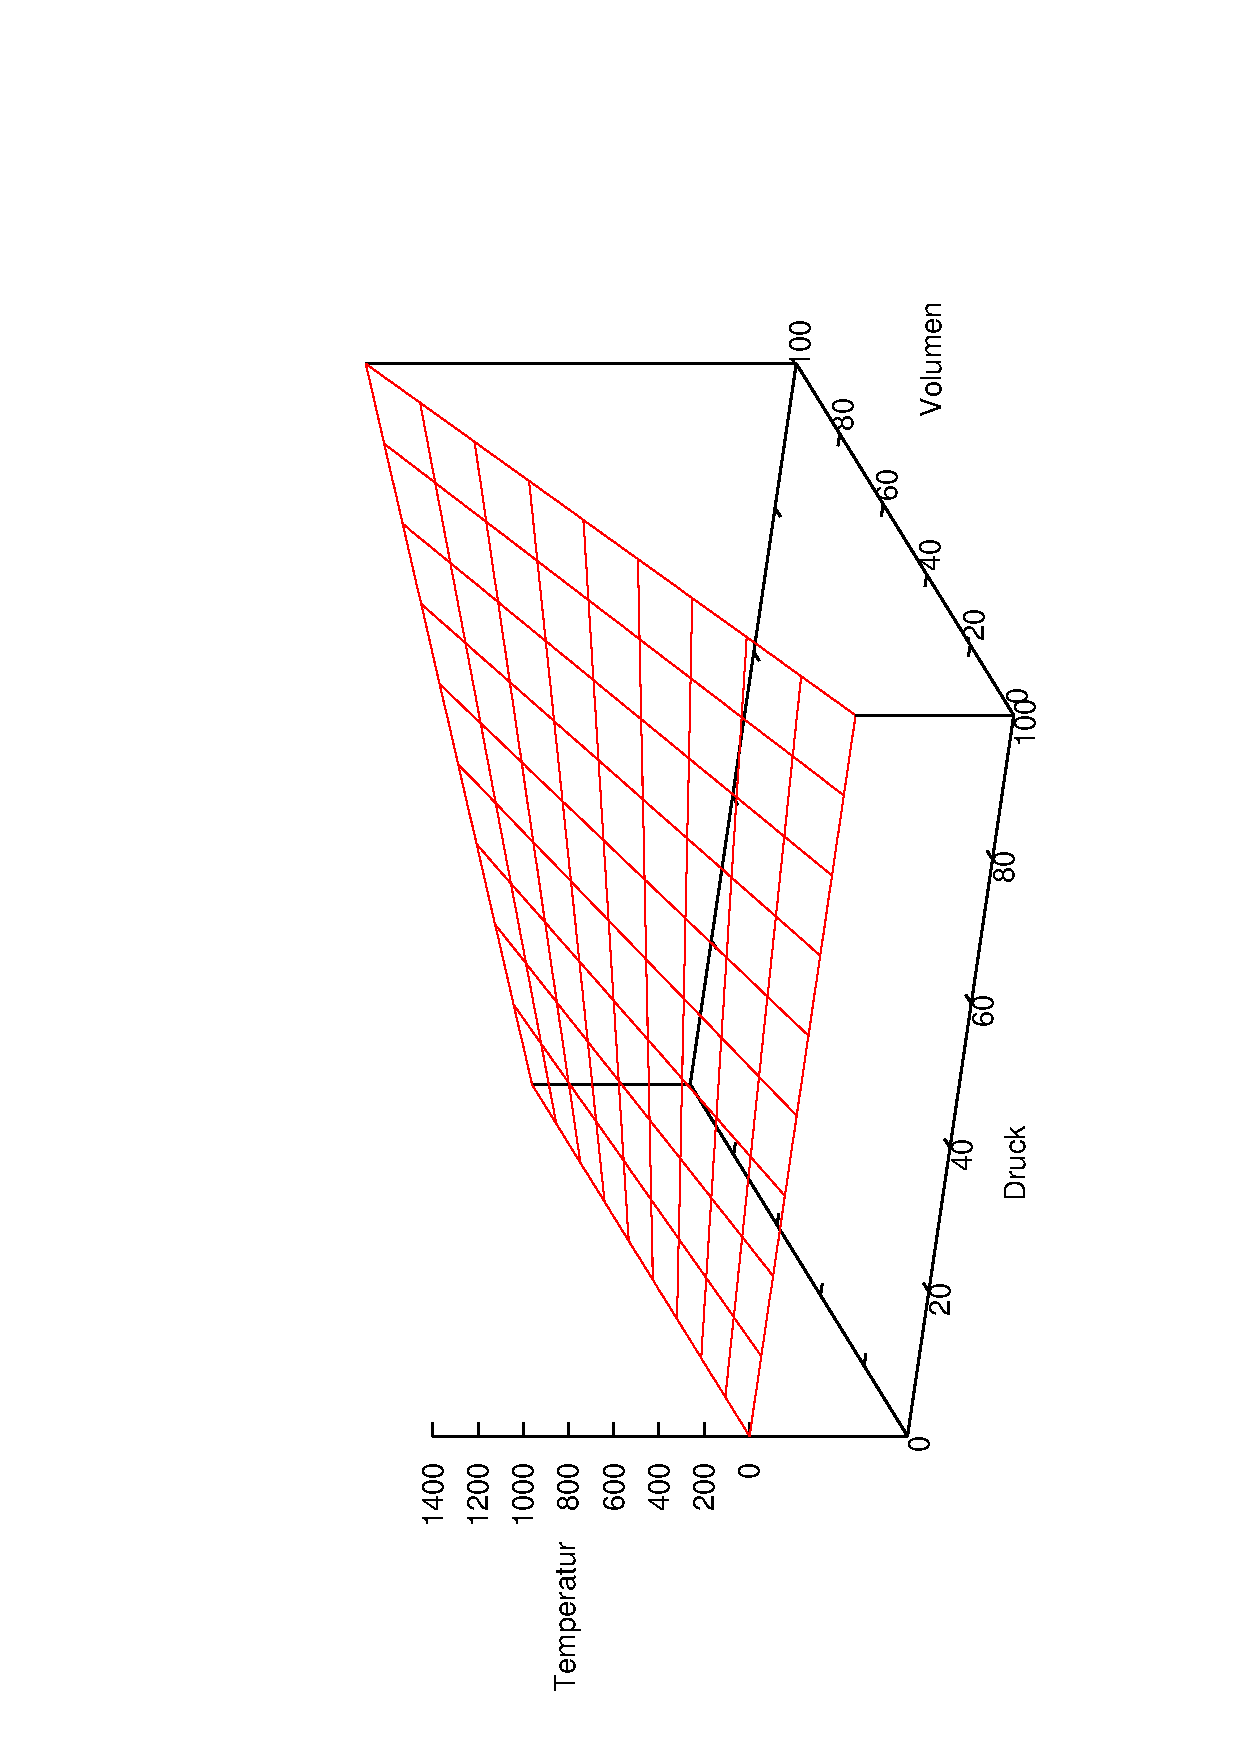
\includegraphics[width=0.34\textwidth,angle=-90]{bilder/gasB1}}  
\subfigure[Volumen gegen Druck (vorne) und Temperatur
   (rechts)]{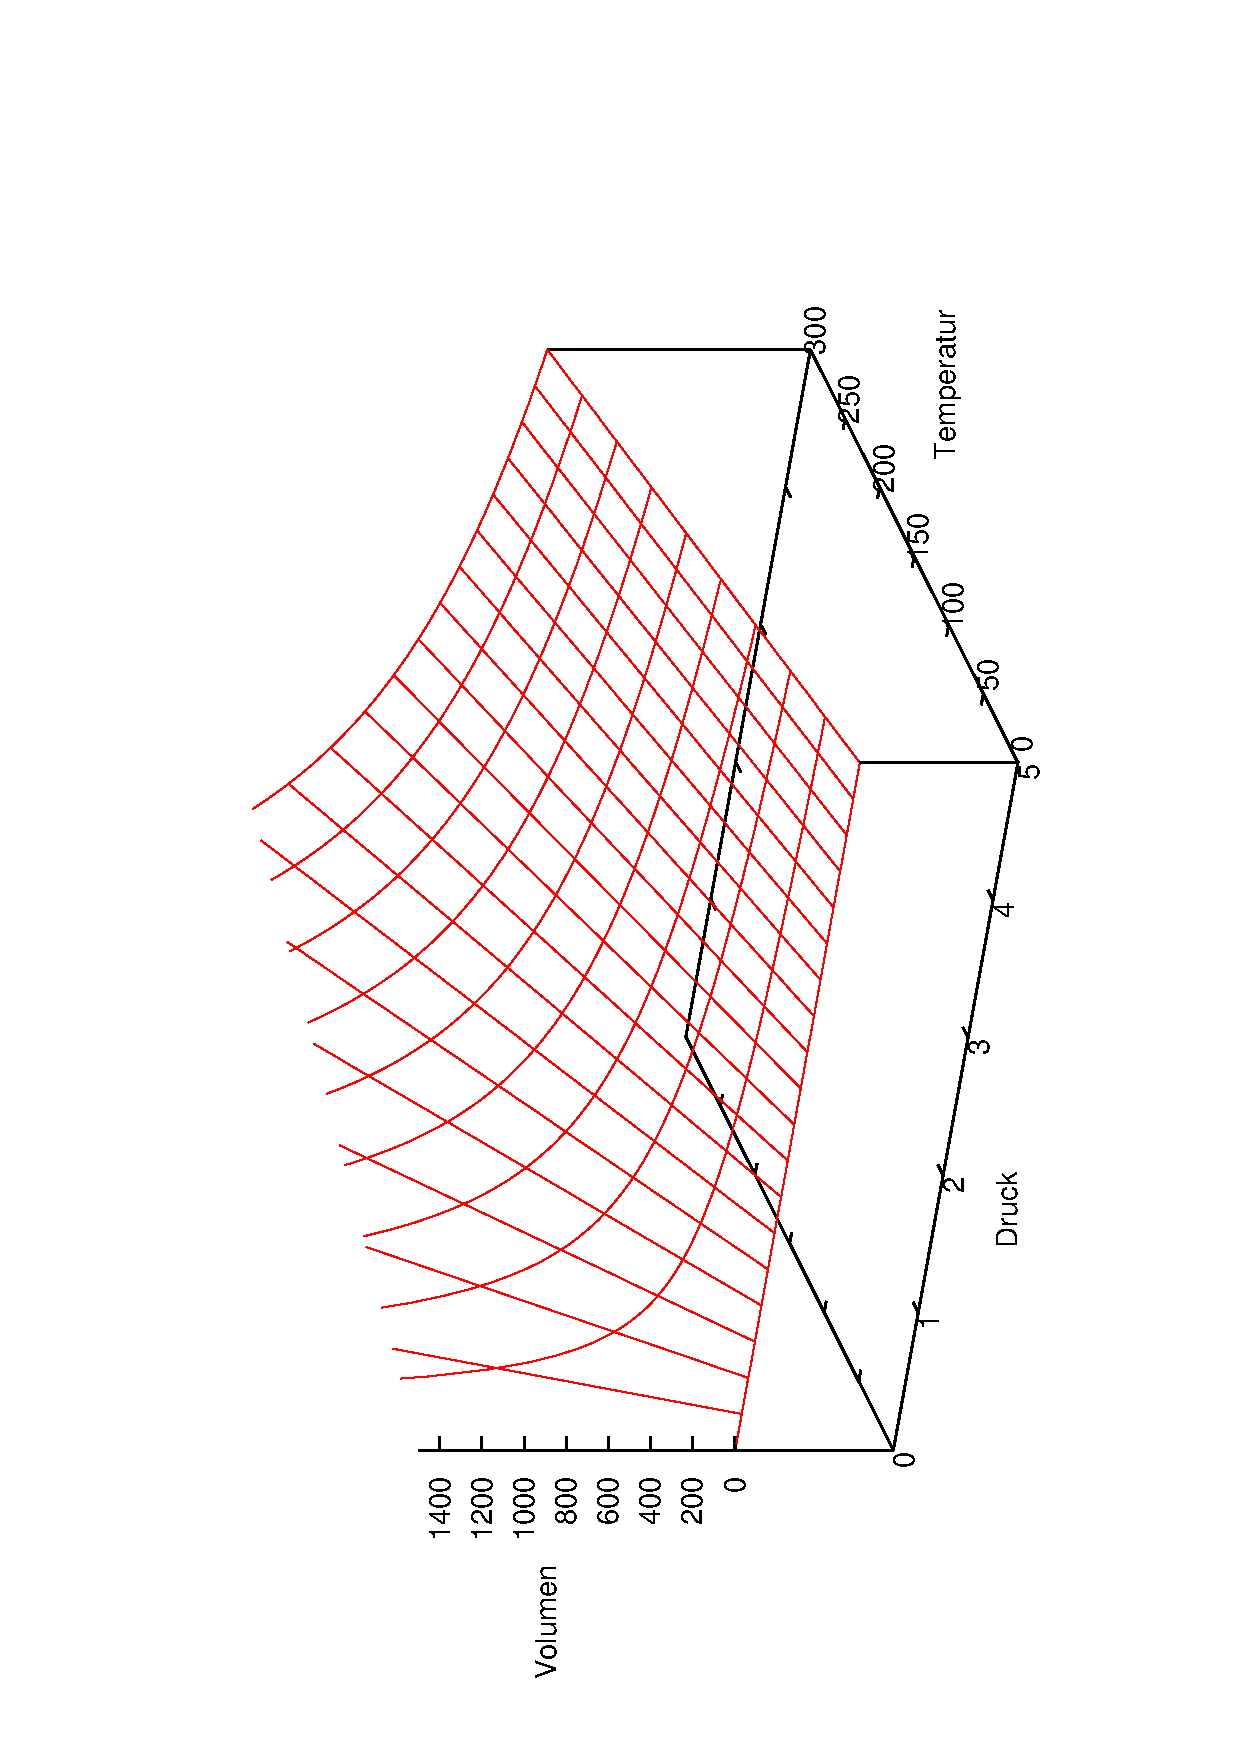
\includegraphics[width=0.34\textwidth,angle=-90]{bilder/gasB2}}
\caption[Flächen der Idealen Gasgleichung]{Fl"ache der Idealen
     Gasgleichung im $\mathbb R^3$ -- Zahlen gelten für $1
     \operatorname{mol}$ Gas. Die eingezeichneten Linien sind Isobare,
     Isotherme bzw. Isochore.}
   \label{abb_ideale-gasgleichung}
\end{figure}

Wir unterscheiden folgende entscheidende F"alle:
\begin{center}
   \begin{tabular}[c]{l l l}
   Isotherm & konstante Temperatur & $\diff T = 0$\\
   Iosbar & konstanter Druck & $\diff p = 0$\\
   Isochor & konstantes Volumen & $\diff V = 0$\\
   Adiabatisch & kein W"armeaustausch & $\diff Q = 0$
\end{tabular}
\end{center}
 Sie sind spezialf"alle
f"ur den \emph{Ersten Hauptsatz der Thermodynamik} (s.
\ref{kap_erste-hauptsatz-thermodynamik}) und k"onenn mit
diesem genauer betrachtet werden. 

\subsection{Isotherm}
\label{kap_isotherm}

Es gilt
$$
T = T_0 = const \text{ oder } {\diff T= 0}
$$
und mit \eqref{eqn_ideale-gasgleichung} folgt 
$$
p \sim \frac{1}{V}
$$
Im Experiment muss das Gas \emph{langsam} komprimiert werden, damit
die entstehende W"arme komplett in ein W"armebad (mit $T = T_0$)
abgegeben werden kann.

Die \textbf{Isotherme \index{Isotherme
    Kompressibilit"at}\index{Kompressibilit"at}Kompressibilit"at}\footnote{Die
Kompressibilit"at $\kappa$ ist uns noch aus
Kap. \ref{kap_krafte-auf-festkorper} bekannt. Dieses $\kappa$ hier ist
der Kehrwert eines \emph{Kompressionsmoduls} ($\kappa = \frac{1}{K}$)
und hat mit dem \emph{Adiabatenkoeffizient} $\kappa$ wenig zu tun.}
\begin{equation}
   \label{eqn_Isotherme-kompressibilit"at}
   \kappa = - \frac{1}{V} \left ( \frac{\partial V}{\partial p} \right )_T
\end{equation}
gibt die relative Volumen"anderung bei konstanter Temperatur pro
Druck"anderung an.

Wie wir schon gesehen haben (in \eqref{eqn_thermische-energie}) h"angt
$U$ alleine von der Temperatur $T$ ab. Ist diese konstant, wie in
diesem Fall, folgt aus $\diff T = 0$ auch $\diff U = 0$.  Weiter folgt mit
\eqref{eqn_erster-hauptsatz-ideales-gas}:
\begin{equation}
   \label{eqn_isotherm_unnere-energie}
   -\diff W = \diff Q = p \cdot \diff V = \frac{nRT}{V}\diff V
\end{equation}
\begin{Wichtig}
Es wird also die komplette, dem System zugef"ugte Energie $\Delta Q$ in
\emph{Volumenarbeit} umgewandelt.   
\end{Wichtig}
%
%
Durch Integration kann man einfach die \emph{Energie} ausrechnen, die
ein Gas verrichtet, welches sich isotherm von $V_1$ auf $V_2$
ausdehnt:
\begin{equation}
   \label{eq:3}
W = - nRT \int_{ V_1 }^{ V_2 } \frac{1}{V}\diff V = nRT \ln \frac{V_1}{V_2}   
\end{equation}




Mit \eqref{eqn_ideale-gasgleichung} folgt schlie"slich noch
\begin{equation}
%   \label{eq:5}
   pV = nRT = const ~\Rightarrow ~ p \sim \frac{1}{V}
\end{equation}
Man spricht hier vom \textbf{\textsc{Boyle}-\textsc{Mariotte}'schen Gesetz}.




\subsection{Isobar}
\label{kap_isobar}

Es gilt
$$
p = p_0 = const \text{ oder } { \diff p = 0}
$$
Und mit \eqref{eqn_ideale-gasgleichung} folgt
$$
V \sim T
$$

Der \textbf{isobare \index{isobarer
Ausdehnungskoeffizient}Ausdehnungskoeffizient}
\begin{equation}
   \label{eqn_isobarer-ausdehnungskoeffizient}
   \gamma_v = \frac{1}{V} \left ( \frac{\partial V}{\partial T }
   \right )_p
\end{equation}
gibt die relative Volumenausdehnung pro Kelvin Temperaturerh"ohung an,
wenn $p = const$.


F"ur ein konstantes $p$ erhalten wir $\diff p = 0$. Nun f"uhren wir (vorl"aufig)
ein:
\begin{Def}
   [\index{Enthalpie}Enthalpie]
Die Enthalpie $H$ ist
\begin{equation}
   \label{eqn_entropie}
   H = U + p \cdot V 
\end{equation}
Sie besteht also aus \emph{Innerer Energie} und
\emph{Volumenarbeit}. Man verwendet $H$, um die \emph{Energie} im
System anzugeben.
\end{Def}

Es gilt nun also f"ur $\diff H$, wenn man
\eqref{eqn_erster-hauptsatz-ideales-gas} einsetzt (und $\diff p = 0$
wegen isobar beachtet):
$$
\diff H = \diff U + V \diff p + p \diff V = \diff Q + V \diff p
$$
und damit
\begin{equation}
   \label{eq:4}
   \diff H = \diff U + p \diff V = \diff Q
\end{equation}
\begin{Wichtig}
   Es wird die komplette zugef"uhrte W"armemenge in Enthalpie imgewandelt.
\end{Wichtig}
Wir k"onnen dies verwenden, um die Spezifische W"arkekapazit"at $C_p$
umzuschreiben; \emph{bei konstantem Druck} gilt:
\begin{equation}
   \label{eqn_Cp}
   C_p = \left ( \frac{\partial H }{\partial T} \right )_p
\end{equation}
Vergleiche Gl. \eqref{eqn_Cv}.






\subsection{Isochore}
\label{kap_isochore}

Es ist 
$$
V = V_0 = const \text{ oder } { \diff V = 0}
$$
 und mit \eqref{eqn_ideale-gasgleichung}
folgt
$$p \sim T$$
Der \textbf{Isochore \index{ioscorer Spannungskoeffizient}Spannungskoeffizient}
\begin{equation}
   \label{eqn_ioscorer-spannungskoeffizient}
   \gamma_p = \frac{1}{p} \left ( \frac{\partial p}{\partial T} \right )_V
\end{equation}
gibt an, wie sich der Druck bei konstantem Volumen vergr"o"sert, wenn
die Temperatur ge"andert wird.

Mit Gl. \eqref{eqn_erster-hauptsatz-ideales-gas} und $\diff V = 0$
gilt
\begin{equation}
   \label{eqn_waerme-aus-waermekapazitaet}
   \diff Q = \diff U = C_V \cdot \diff T
\end{equation}
\begin{Wichtig}
D.h. die zugef"uhrte W"armemenge wird \emph{vollst"andig} in innere
Energie umgesetzt.    
\end{Wichtig}
Hier kann man jetzt definieren:
\begin{equation}
   \label{eqn_Cv}
   C_V = \left ( \frac{\partial U}{\partial T} \right )_V
\end{equation}
Vgl. Gl. \eqref{eqn_Cp}.



% \subsection{Volumen"anderung}
\subsection{Zusammenhang zwischen den Koeffizienten}
\label{kap_zusammenhang-zwischen-den-koeffizienten}
\label{kap_volumenanderung}

Die komplette Volumen"anderung eines Volumens $V(p,T) = V_0$ schlie"slich
ergibt sich bei einer "Anderung von $T$ und $p$ mit
\eqref{eqn_Isotherme-kompressibilit"at}  und
\eqref{eqn_isobarer-ausdehnungskoeffizient} zu
$$
\diff V = \left ( \frac{\partial V}{\partial p} \right )_T \diff p +
\left ( \frac{\partial V}{\partial T } \right )_p \diff T =
- \kappa \cdot V_0 \cdot \diff p + \gamma_V \cdot V_0 \cdot \diff T
$$
Bei isochoren Prozessen bleibt das Volumen konstant ($\diff V = 0$) und
man bekommt hierf"ur
$$
\kappa \cdot \diff p = \gamma_V \diff T
$$
%
%
Und so erh"alt man durch Division durch $\diff T$ und mit
Gl. \eqref{eqn_ioscorer-spannungskoeffizient} schlie"slich als
Zusammenhang zwischen den Koeffizienten:
\begin{equation}
   \label{eqn_zshg-koeffizienten}
   \kappa \cdot \gamma_p \cdot p = \gamma_V 
\end{equation}




\subsection{Adiabate}
\label{kap_adiabate}

Es findet \emph{kein W"armeaustausch} mit der Umgebung statt; also
ist 
$$
Q = Q_0 = const \text{ oder } {\diff Q = 0}
$$
In der Natur finden solche Vorg"ange h"aufig als \emph{Grenzf"alle}
statt; wenn sich der Zustand eines Gases so schnell "andert, dass das
Gas einfach keine Zeit hat, mit der Umgebung W"arme auszutauschen --
bzw. nur vernachl"assigbar wenig.

F"ur den 1. HS \eqref{eqn_erster-hauptsatz-ideales-gas} folgt (mit
\ref{eqn_Cv}) da $\diff Q = 0$:
\begin{equation}
   \label{eq:1}
   \diff U = - p \diff V = C_V \diff T
\end{equation}
Verwenden wir nun noch \eqref{eqn_ideale-gasgleichung} und ersetzen $p
= \frac{nRT}{V}$ und nach \eqref{eqn_c_v} $C_V = \frac{f}{2} K_BN$ so
gilt (nach anschlie"sender Integration):
\begin{eqnarray}
\nonumber
\frac{f}{2} K_B N \diff T &=& - \frac{NK_BT}{V} \diff V   \\
\nonumber
\frac{f}{2}  \cdot \frac{1}{T} \diff T &=& -   \frac{1}{V}
\diff V   \\
\nonumber
\frac{f}{2}  \int \frac{1}{T} \diff T &=& - \int \frac{1}{V}
\diff V  \\
\nonumber
\frac{f}{2} \ln T &=& - \ln V + \const \\
\nonumber
\ln (  T^{ \frac{f}{2} } \cdot V ) &=& \const \\
\label{eq:7}
T^{ \frac{f}{2} } \cdot V  &=& \const 
\end{eqnarray}
Die Gleichung kann man noch mit $K_BN$ potenzieren und erh"alt unter
Beachtung von \eqref{eqn_differenz-c}:
\begin{equation}
   \label{eq:6}
   T^{ C_V } \cdot V^{ (C_P - C_V) }  = \boxed {T\cdot V^{ \kappa - 1
     }= const }
\end{equation}
Alternativ kann man aus \eqref{eq:7} mit \eqref{eqn_ideale-gasgleichung} $T$
ersetzen
(und ein paar Konstanten k"urzen). Beachtet man nun, dass $V\cdot V^{
  \frac{2}{f}} = V^{ \frac{2+f}{f} }$ ist und verwendet
\eqref{eqn_adiabatenkoeffizient} statt $\frac{2+f}{f}$, so erh"alt man
\begin{equation}
   \label{eq:9}
\boxed{
   pV^\kappa = const
}
\end{equation}
(Dieses Ergebnis h"atte man auch erhalten, h"atte man mit
\eqref{eqn_ideale-gasgleichung} das $TV^{\kappa-1 } =
\frac{T}{V}V^\kappa$ das $\frac{T}{V}$ ersetzen k"onnen.)




\subsection{Erw"armung bei adiabatischer Kompression}
\label{kap_erwarmung-bei-adiabatischer-kompression}

F"ur isotherme Prozesse gilt $pV = const$ und f"ur adiabatsiche
$pV^\kappa = const$. (In einem $V$-$p$-Diagramm\footnote{also $p$ auf
  der $x$-Achse und $V$ auf der $y$-Achse} sind die Isothermen steiler
als die Adiabaten.) Es liegt also nahe, diese beiden Prozesse zu
vergleichen. Siehe dazu Abb. \ref{abb_isotherm-adiabatisch}: Die
Adiabate schneidet die beiden Isothermen an zwei Stellen. Bei
adiabatischer Kompression -- also wenn wir einer Adiabaten folgen --
wechseln wir folglich von der niedrigen auf die h"ohere Isothermen und
folglich muss sich die Temperatur bei der Kompression erh"ohen.

Das kommt daher, dass bei der Kompression mechanische Arbeit in W"arme
umgewandelt wird. Beim isothermen Prozess ist es nun so, dass diese
W"arme abgegeben werden kann, beim adiabatischen dagegen verbleibt
diese W"arme im Gas und sorgt hier daf"ur, dass die Temperatur steigt.

% \begin{figure}
%    \centering
% 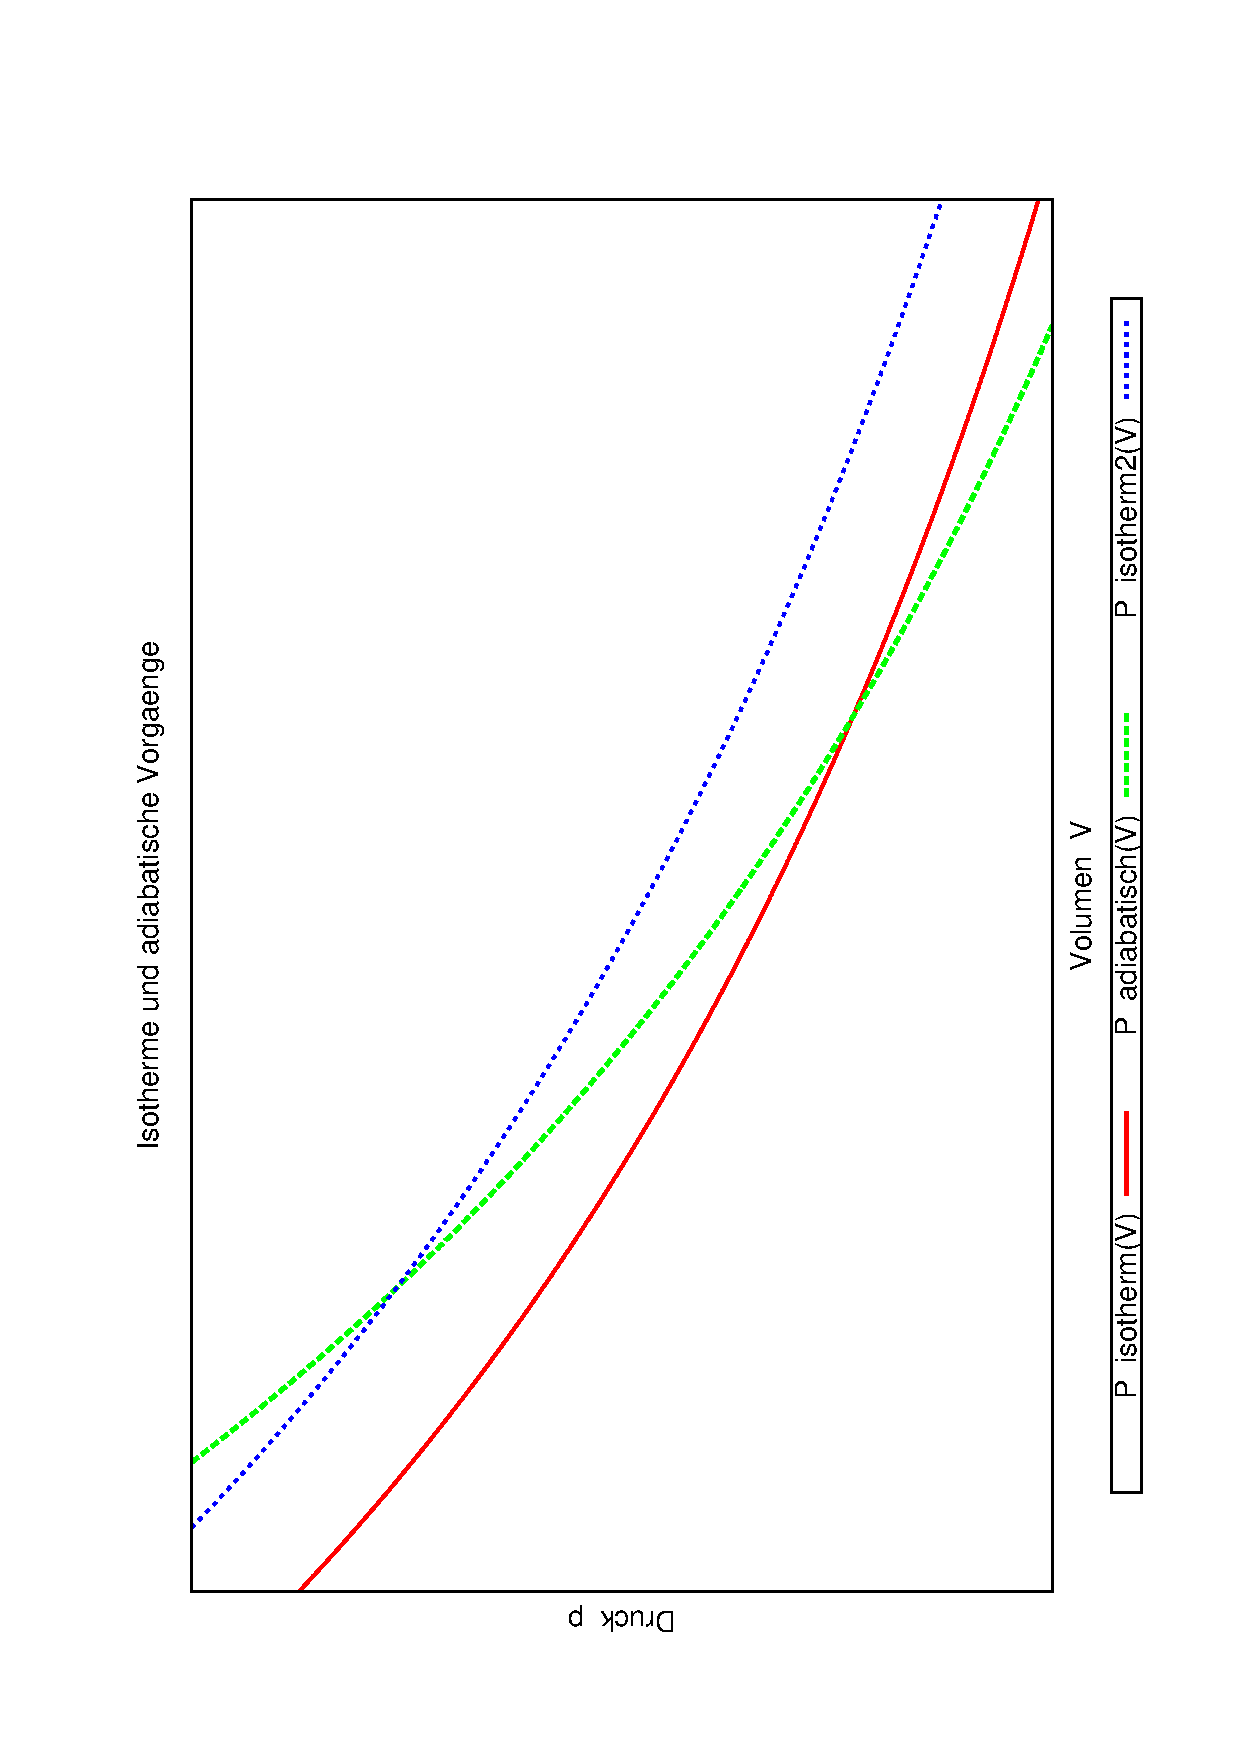
\includegraphics[width=0.5\textwidth,angle=-90]{bilder/iso-adiab}
%    \caption{Abbildung eines adiabatischen und zweier Isothermer Prozesse}
%    \label{abb_isotherm-adiabatisch}
% \end{figure}












\section{Zweiter Hauptsatz}
\label{kap_zweiter-hauptsatz}

W"arend der erste Hauptsatz noch die Energieerhaltung postuliert,
beschreibt der zweite Hauptsatz, \emph{wie} sich die Energieformen
ineinander umwandeln k"onnen.

Wir f"uhren dazu die Entropie ein:

\begin{Def}
   [\index{Entropie}Entropie]
Die Entropie $S$ ist eine Zustandsgr"o"se, die zunimmt, wenn sich ein
System einem Gleichgewichtszustand ann"ahrt. 
\end{Def}
Es gilt 
%bei \emph{reversiblen} Prozessen (mit
%\eqref{eqn_erster-hauptsatz} und der Idealen-Gas-Gleichung):
dabei mit der reversiblen W"armemenge:
\begin{equation}
   \label{eqn_def_entropie}
   \diff S = \frac{\diff Q_\text{rev}}{T} 
% =
%  \frac{\diff U + p \diff V}{T}
% =
% \frac{\frac{f}{2} N K_B  \diff T}{T} + \frac{N K_B \diff V}{V}
\end{equation}

Eigentlich setzt sich $\diff S$ zusammen aus einem
\emph{Entropiefluss} $\diff S^\text{e}$ von Au"sen in das System und
einer inneren \emph{Entropieproduktion} $\diff S^\text{i}$ durch
Prozesse im Inneren des Systems:
\begin{equation}
 \diff S = \diff S ^\text{e} + \diff S^\text{i}
\end{equation}
Analog zu Gl. \eqref{eqn_def_entropie} k"onnte man schreiben:
\begin{equation*}
   \diff S^\text{e} = \frac{\diff Q}{T}
\end{equation*}
wobei diesmal $\diff Q$ die gesamte mit der Umgebung ausgetauschte
W"armemenge ist. 

Mit der Definition folgt:
\begin{description}[\setlabelstyle{\bfseries\slshape}]
\item[$\Delta S > 0$] \index{irreversibler}irreversibler Prozess
\item[$\Delta S = 0$] \index{reversibler}reversibler Prozess
\item[$\Delta S < 0$] Wird in der Natur nicht beobachtet (zumindest
   nicht in \emph{makroskopischen} Systemen.
\end{description}
Die W"armemenge
\begin{equation*}
   \Delta Q = T \cdot \Delta S
\end{equation*}
die bei einem Prozess frei wird, bezeichnet man auch als
\emph{\index{Abw"arme}Abw"arme} oder
\emph{\index{Verlust-Energie}Verlust-Energie}, weil sie bei dem
Prozess nur zur "Anderung der Entropie verwendet wird, nicht aber, um
wirklich Arbeit zu verrichten.

Wir k"onnen sagen, dass die Entropie die \textbf{Zahl der Zust"ande}
eines Systems ist. F"uhrt man in diesem System eine
\index{Zwangsbedingung}Zwangsbedingung ein, so reduziert man die
m"ogliche Zahl der Zust"ande und \emph{erniedrigt} damit die
Entropie. Um das System auf diese Zwangsbedingungen zu bringen, sind
aber Zwangs\emph{kr"afte} n"otig. Man muss Arbeit investieren, um das
System in den neuen, mit den Zwangsbedingungen vertr"aglichen Zustand
zu bringen.

\begin{Beispiel}
   Bei dem ber"uhmten Beispiel eines Kastens der zur H"alfte mit Gas
   gef"ullt ist, haben wir die Zangsbedingung der Trennung. Wird die
   Trennung weggenommen -- also die Zwangsbedingung aufgehoben --
   verteilt das Gas sich im ganzen, ihm zur Verf"ugung stehenden Raum,
   und maximiert so seine Entropie. M"ochte man den urspr"unglichen
   Zustand wieder herstellen, so muss man \emph{von Au"sen} Energie
   investieren, um die Teilchen wieder zur"uckzusortieren.
\end{Beispiel}


Ebenso kann man die Entropie als \textbf{Informationsgehalt}
verstehen: Je gr"o"ser die Information, desto kleiner die Entropie. 
\begin{Beispiel}
   In dem halbvollen Kasten ist der Informationsgehalt h"oher: Man kann
   mit absoluter Sicherheit f"ur jedes Teilchen einen Punkt
   "`irgendwo"' innerhalb von $\frac{1}{2}V$ annehmen. Bei dem gro"sen
   Kasten dagegen kann man f"ur die Teilchen nur noch sagen, sie
   befinden sich "`irgendwo"' in $V$. Der Informationsgehalt hat also
   vom halbvollen zum vollen Kasten so \emph{ab}genommen, wie die
   Entropie \emph{zu}genommen hat.
\end{Beispiel}

Nicht ganz korrekt, aber daf"ur anschaulich, kann
man sagen, dass die Entropie ein \emph{Ma"s f"ur die Unordnung} eines
Systems ist.

\abs 
Wie wir in Kap. \ref{kap_reversible-und-irreversible-prozesse}
sehen werden, strebt die Natur zu einem \emph{Gleichgewicht}; sie ist
also bestrebt, dass $\Delta S > 0$ ist. Man k"onnte also sagen, sie
ist bestrebt, die Entropie zu maximieren.

So ist auch der zweite Hauptsatz zu verstehen:
\begin{Wichtig}
   [\index{Zweiter Hauptsatz der Thermodynamik}Zweiter
   \index{Hauptsatz Thermodynamik}Hauptsatz der Thermodynamik]
In einem abgeschlossenen (adiabatischen) System kann die Entropie
nicht ab-, sondern nur zunehmen, und bleibt h"ochstens bei reversiblen
Prozessen konstant:
\begin{equation}
   \label{eqn_zwetier-hauptsatz}
   \boxed{
\Delta S \geq 0
}
\end{equation}
\end{Wichtig}
Man kann ihn auch umformulieren:
\begin{quote}
   W"arme flie"st von selbst nur von w"armeren zu k"alteren Stellen --
   niemals umgekehrt
\end{quote}

Interessant ist noch, dass bei einem irreversibel ablaufenden,
adiabatischen Prozess Entropie $\diff S^\text{i}$ im System erzeugt
wird, bei einem reversiblen logischerweise nicht; Entropie"anderung
(\emph{-fluss} $\diff S^\text{e}$) von au"sen wird aber in keinem der
F"alle ins System gebracht.

% Wiki: Adiabatische_Zustands"anderung






\section{Dritter Hauptsatz}
\label{kap_dritter-hauptsatz}

Der Dritter Hauptsatz ist sehr schlicht:
\begin{Wichtig}
   [Dritter \index{Hauptsatz Thermodynamik}Hauptsatz der \index{Dritter Hauptsatz der
     Thermodynamik}Thermodynamik]
Es ist nicht m"oglich, ein System bis auf $T =0$ abzuk"uhlen.
\end{Wichtig}
Au"serdem gilt f"ur die Entropie:
$$
S(T,p,V) \stackrel{T \to 0}{\to} S_0
$$
d.h. wenn $T$ verschwindet, so geht $S$ unabh"angig von den anderen
Parametern $p$, $V$, ... gegen den Zustand $S_0$ wobei f"ur diesen
gilt:
$$
S_0 =K_B \ln \Omega_0 
$$
wobei $\Omega_0$ die Anzahl m"oglicher Mikrozust"ande im System
darstellt.

F"ur alle physikalisch-chemischen Reaktionen, bei denen die
teilnehmenden Stoffe am absoluten Nullpunkt als ideale kristalline
Festk"orper vorliegen, gilt:
$$
S_0 = 0
$$
und damit folgt $ln \Omega_0 = 0$ bzw. $\Omega_0 = 1$. Es gibt also
nur einen einzigen Zustand, den das System am absoluten Nullpunkt
einnehmen kann.









\section{Freie Energie und Enthalpie}



\subsection{Freie Energie}
\label{kap_freie-energie}



In der \emph{Mechanik} versuchen (makroskopische) K"orper ihre
(potentielle) Energie zu minimieren: Ein K"orper f"allt so weit er kann
nach "`unten"', damit die potentielle Energie m"oglichst klein wird. In
der \emph{Thermodynamik} ist dies offensichtlich nicht so -- sonst
w"urden sich alle Luftteilchen m"oglichst nahe "uber dem Boden befinden
und weiter oben g"abe es keine Luft mehr.

Um diesen Drang der Natur nach einem Energieminimum weiterhin als
physikalische Regel beibehalten zu k"onnen, m"ussen wir eine Art
\emph{thermodynamisches Potential} definieren:

\begin{Def}
   [\index{Freie Energie}Freie Energie $\mathcal F$]
Die Freie Energie $\mathbf \mathcal{F}$ ist definiert als
\begin{equation}
   \label{eqn_freie-energie}
\boxed{
  \mathcal F = U - T \cdot S
}
\end{equation}
mit der Entropie $S$ und der Inneren Energie $U$.  

Wir bezeichnen $\mathcal F$ auch als \textbf{\index{Thermodynamisches
    Potential}thermodynamisches Potential}.
\end{Def}
%
Im Gegensatz zur freien Energie, bezeichet man als \textbf{gebundene
  Energie}:
\begin{equation}
   \label{eqn_gebundene-energie}
 TS =    U - \mathcal F
\end{equation}
\begin{Wichtig}
   [Freies \index{Freies Energieminimum}Energieminimum] Die Natur ist
   (bei konstantem Volumen -- also bei einem \emph{mechanisch
     isolierten} System -- und konstanter Temperatur) bestrebt, dass
   die \textbf{freie Energie $\mathcal F$ minimal} wird. Dies
   entspricht dem Gleichgewichtszustand.
\end{Wichtig}

Vergleichen wir das mit dem zweiten Hauptsatz der Thermodynamik
(Kap. \ref{kap_zweiter-hauptsatz}), der besagt, dass $S$ maximal
werden soll, sehen wir, dass diese beiden in Einklang stehen: Wird $S$
gr"o"ser, so wird $\mathcal F$ wegen des Minuszeichens in
\eqref{eqn_freie-energie} kleiner.

% Betrachten wir nun isotherme Zustands"anderungen (bei denen also
% $\diff T = 0$ und mit Gl. \eqref{eqn_thermische-energie} auch $\diff
% U = 0$) ist, so gilt

\begin{Wichtig}
   Es wird sich stets ein Gleichgewicht -- bzw. ein \emph{Kompromiss}
   zwischen der Maximierung von $S$ und der Minimierung von $\mathcal
   F$ geben.\footnote{Mimimierung von $\mathcal F$: Gasteilchen
     bewegen sich nicht mehr uns liegen am Boden ($\mathcal F$ min \Ipl $N\bar
     u$ min \Ipl $\bar u$ min \Ipl $\bar v$ min)\\Maximierung von $S$:
     Teilchen verteilen sich homogen; nehem m"oglichst viel Platz
     ein.}  Dieser Kompromiss ist die \textsc{Boltzmann}-Verteilung
   (Kap.  \ref{kap_exkurs:bolzmann-faktorn-und-thermische-energie}).
\end{Wichtig}





\subsection{Freie Enthalpie}
\label{kap_freie-enthalpie}

Analog zur Freie Energie definiert man in einem Sysem f"ur die Enthalpie:
\begin{Def}
   [Freie Enthalpie $G$] 
   \begin{equation}
      \label{eq:207}
      G = H - TS
   \end{equation}
Es handelt sich dabei um ein weiteres \textbf{\index{Thermodynamisches
  Potential}Thermodynamisches Potential}
\end{Def}



\begin{Wichtig}
   [\index{Freies Enthalpieminimum}Freies Enthalpieminimum] Bleiben
   Druck und Temperatur eines Systems konstant, ist die Natur
   bestrebt $G$ zu minimieren.
\end{Wichtig}
Dieser Satz wird h"aufig in der Chemie gebraucht, weil hier die meisten
Reaktionen bei (konstantem) Druck ablaufen (in offenen Gef"a"sen). Man
sieht hier: Eine Reaktion l"auft nur dann ab, wenn $\Delta G < 0$
ist. Der Chemiker bezeichnet dies als \emph{exergonische}
Reaktion. Im Gegensatz dazu ben"otigen \emph{endergonische} Reaktionen
mit $\Delta G > 0$ \emph{Energiezufuhr}.









\section{Kreisprozesse}
\label{kap_kreisprozesse}

\begin{Def}
   [\index{Kreisprozess}Kreisprozess] Ein thermodynamisches System
   durchl"auft verschiedene Zust"ande, kommt anschlie"send aber wieder
   zum Ausgangszustand zur"uck: Es hat wieder die selben
   Zustandsgr"o"sen.
\end{Def}

Bei einem Kreisprozess bleibt die Innere Energie $U$ \emph{zwischen
  Anfangs- und Endzustand} erhalten: $U_a = U_e$ bzw. $\Delta U = 0$
(wobei sich das "`$\Delta $"' auf dem gesamten Prozess bezieht). Mit
dem ersten HS \eqref{eqn_erster-hauptsatz} folgt so:
$$
 \Delta Q = - \Delta W
$$
Es wird also alle aufgenommene W"arme direkt in Arbeit umgesetzt (und
anders herum). Das "`$-$"' bedeutet hier, dass wenn man W"arme in das
System hineinsteckt, man Arbeit verrichtet bekommt, und anderst herum
eine W"armemenge erh"alt, wenn man an dem System Arbeit verrichtet. Wir
bezeichnen solche Systeme auch als
\textbf{\index{W"armekraftmaschinen}W"armekraftmaschinen}. Sie k"onnen
(nur) arbeiten, wenn ihnen st"andig W"arme zugef"uhrt wird.


\subsection{Reversible und Irreversible Prozesse}
\label{kap_reversible-und-irreversible-prozesse}

Wir unterscheiden bei Kreisprozessen, ob ein Prozess re- oder
irreversibel ist. Kann er in beiden Richtungen ablaufen, so hei"st er
\emph{reversibel}, kann er nur in einer Richtung ablaufen, so ist er
\emph{irreversibel}. In der Natur kommen erstere h"ochstens auf der
mikroskopischen Scala vor -- im makroskopischen Bereich bleiben
reversible Prozesse leider Gedankenexperimente.
\begin{Wichtig}
   Thermodynamische Prozesse laufen h"aufig nur in eine Richtung von
   selbst ab.
\end{Wichtig}

\begin{Beispiel}
   Haben wir bspw einen Kolben, dessen Innendruck den Au"sendruck
   "ubersteigt, so wird der Kolben herausgeschoben und verrichtet so
   Arbeit. Der Umgekehrte Fall ist zwar nach dem ersten Hauptsatz der
   Thermodynamik m"oglich, wird in der Natur jedoch nicht eintreten.
\end{Beispiel}


Eine gute Erkl"arung daf"ur ist, dass der ausgedehnte Kolben ein
\emph{Gleichgewichtszustand} ist. Die Natur ist bestrebt, diesen
Gleichgewichtszustand einzustellen -- jedoch alles andre als bestrebt,
diesen wieder zu verlassen; der Prozess ist also folglich
\emph{irreversibel}. Dies motiviert den zweiten Haupsatz
(Kap. \ref{kap_zweiter-hauptsatz}).







\subsection{Der \textsc{Carnot}-Prozess}
\label{kap_carnot-prozess}

Es handelt sich hierbei um einen \emph{fundamentalen
  Kreisprozess}, in dem die vier Zust"ande A bis D periodisch
durchlaufen werden. Wir betrachten 
\begin{itemize}
\item einen Gasbeh"alter mit Kolben, in dem das Gas
   ("`\textbf{Arbeitsgas}"') komprimiert bzw. expandiert wird.
\item Der Beh"alter wird abwechselnd in W"armeb"ader unterschiedlicher
   Tempetarturen getaucht: $T_w$ f"ur warme und $T_k$ f"ur kalte B"ader.
\end{itemize}


\begin{figure}
   \centering
   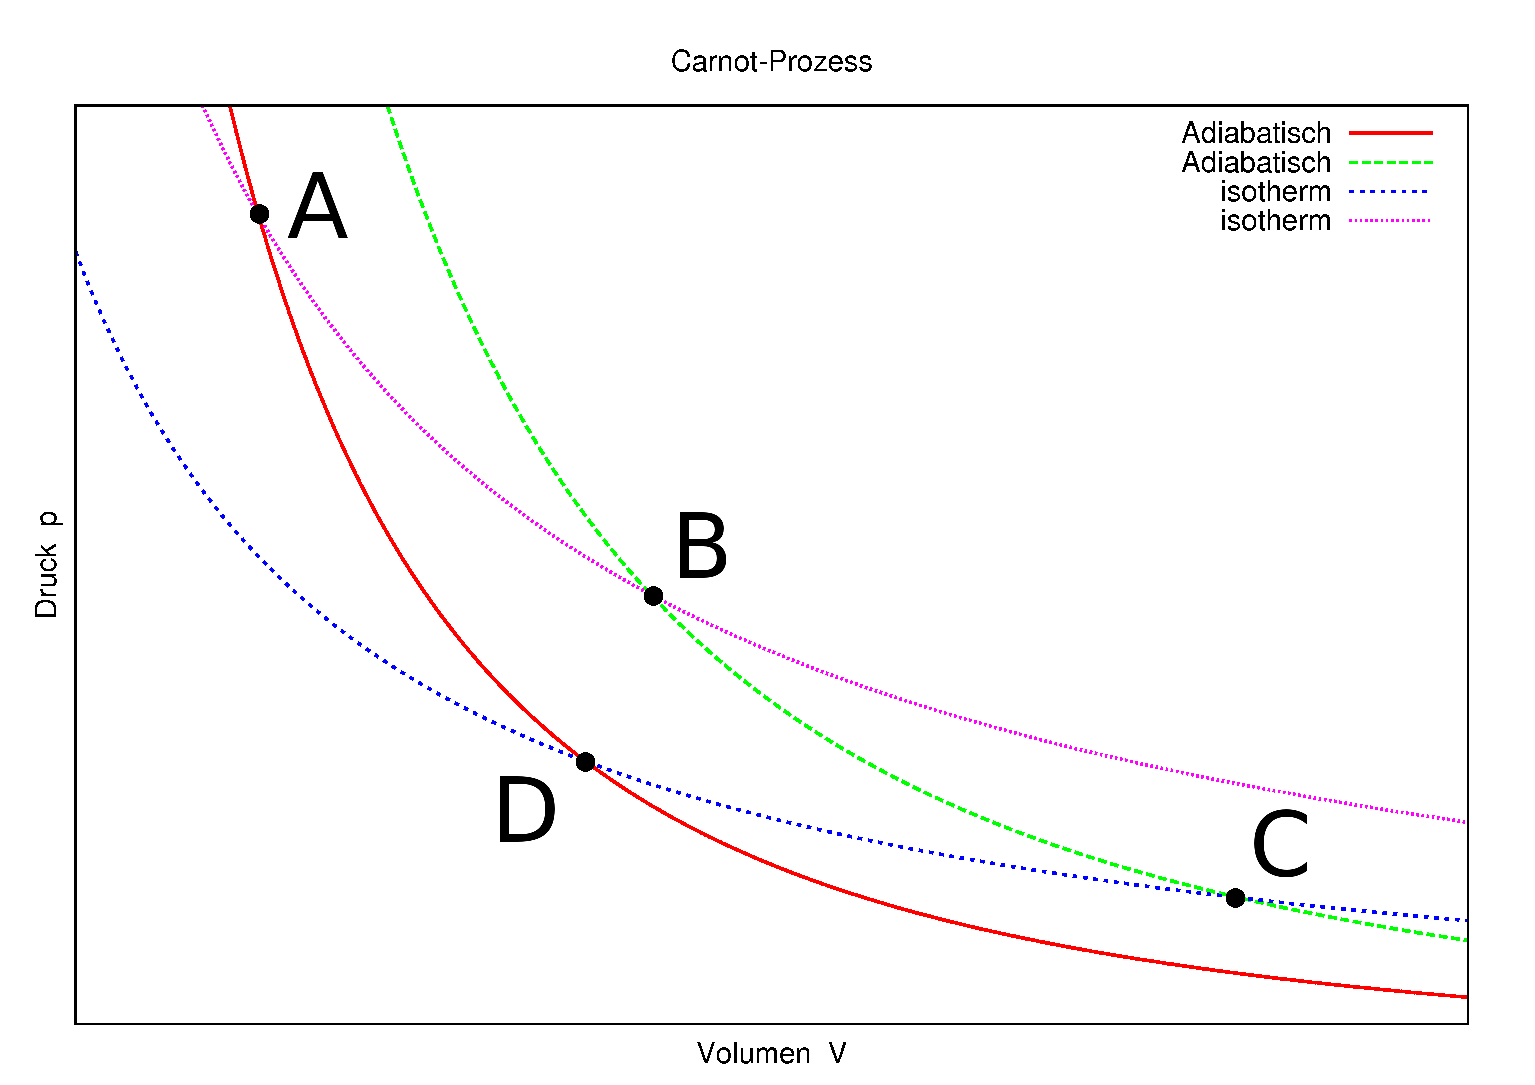
\includegraphics[width=0.7\textwidth]{bilder/carnot1_mod1}
   \caption[Phasendiagramm: Carnot-Prozess]{$p$-$V$-Diagramm des
     Carnot-Prozesses. Die beiden steilen Kurven geh"oren zu
     Adiabatischen Vorg"angen, die flachen zu isothermen. Verwendet
     man ein $V$-$p$-Diagramm tauschen Adiabaten und Isothermen die
     Position.}
   \label{abb_carnot-prozess}
   \label{abb_isotherm-adiabatisch}
% Das Zweite Label ist da, um eine fr"uhere, 
% langweiligere Graphik einzusparen.
\end{figure}


Im einzelnen geschieht (In Abb. \ref{abb_carnot-prozess} sind die vier
Zust"ande A bis D markiert. Die jeweiligen Vorg"ange hier sind also die
jeweiligen Verbindungslinien zwischen den Punkten.):
\begin{description}[\setlabelstyle{\bfseries\slshape}]
\item[A$\to$B Isotherme Expansion] 
Da $T = const$ folgt $\diff T = 0$. Da $U \sim T$
(s. \eqref{eqn_thermische-energie}) ist $\diff U = 0$ und mit dem
1. HS \eqref{eqn_erster-hauptsatz} folgt:
$$
 \diff U = \diff Q + \diff W = 0 ~ \Rightarrow ~ \diff Q = -
 {\diff W} = {p \diff V}
$$
Das Gas nimmt aus dem Reservoir die W"armemenge $\Delta Q_w$ auf und
leistet (damit) die Expansionsarbeit $\Delta W_{AB}$. Es gilt
$$
\Delta W_{ AB } = -\int_{ V_A }^{ V_B } \frac{RT_w}{V}\diff V = -RT_w \ln
\frac{V_B}{V_A} = RT_w \ln\frac{V_A}{V_B} = -\Delta Q_{ w }
$$
Im $\ln$ ist $\frac{V_A}{V_B} < 1$ und damit der $\ln$ negativ: Es
wird wirklich $\Delta W_{AB}$ frei.


\item[B$\to$C adiabatische Expansion] 
Diesmal ist $\diff Q = 0$ und damit mit dem ersten HS: 
$$
%C_V \diff T = \diff U = \diff W = p \diff V
\diff U = \diff W = \frac{f}{2} R \diff T
$$
Und mit $\diff T = T_k - T_w$ und $\frac{f}{2}R = C_V$ folgt:
$$
\Delta W_{ BC } = \int_{ T_w }^{ T_k } C_V \diff T = C_V(T_k - T_w)
$$
Die Differenz rechts ist negativ: Das Gas leistet die
Expansionsarbeit. Die Arbeit kommt dabei aus der Inneren Energie $U$
des Gases.


\item[C$\to$D isotherme Kompression] 
Es ist wieder $\diff T = 0$, nur wird diesmal die Kompressonsarbeit
$\Delta W_{ CD }$ in das Gas gesteckt und die W"armemenge $\Delta Q_k$
wird ans W"armebad abgegeben. Analog zu AB gilt:
$$
\Delta W_{ CD } = -RT_k \ln \frac{V_D}{V_C} = -\Delta Q_k
$$
Da der Quotient $\frac{V_D}{V_C} < 1$ ist der $\ln$ wieder negativ --
damit $\Delta W$ \emph{positiv} und es wird wirklich die Arbeit
$\Delta W$ am Gas geleistet.


\item[D$\to$A adiabatische Kompression] 
Es ist wieder $\diff Q = 0$ und analog zu BC gilt
$$
 \Delta W_{ DA } = C_V(T_w - T_k)
$$
D.h. es wird diesmal wegen $\Delta W > 0$ Arbeit ins Gas gesteckt.
\end{description}



% Insgesamt kann man also die Energiebilanz aufstellen (wir n"utzen aus,
% dass in BC und DA die Energien sich genau wegk"urzen):
% $$
% W = \sum_{A,B,C,D} \Delta W = nRT_w \ln\frac{V_A}{V_B} + nRT_k \ln
% \frac{V_C}{V_D}
% $$

\bigskip
\noindent
Nun wollen wir bilanzieren: Die Arbeit bei DA und BC ist praktisch die
selbe -- wir wollen sie also nicht weiter beachten. Die Gesamtarbeit,
die das System verrichtet hat, sei $W$ und f"ur $W$ gilt:
\begin{equation}
   \label{eq:8}
   W = \sum_{AB,BC,CD,DA} \Delta W = nRT_w \ln\frac{V_B}{V_A} + nRT_k \ln
\frac{V_D}{V_C}
\end{equation}
F"ur die adiabatischen Prozesse BC und DA gilt nun nach \eqref{eq:9}:
\begin{eqnarray}
\nonumber
   T_wV_B^{ \kappa-1 } &=& T_k V_C^{ \kappa-1 }\\
\nonumber
   T_wV_A^{ \kappa-1 } &=& T_k V_D^{ \kappa-1 }\\
\label{eq:11}
\frac{V_B}{V_A} &=& \frac{V_C}{V_D}
\end{eqnarray}
In Gl. \eqref{eq:8} gilt also $\ln\frac{V_B}{V_A} = -\ln
\frac{V_D}{V_C}$ und weiter
\begin{equation}
   \label{eq:12}
\boxed{ W =  nR\cdot(T_w - T_k)\cdot \ln \frac{V_B}{V_A} }
\end{equation}
Dies ist also die Arbeit, die beim Carnot-Prozess verrichtet
wurde. \emph{Graphisch} findet man sie wieder, wenn man die Fl"ache in
Abb. \ref{abb_carnot-prozess} betrachtet, die von den vier Kurven
zwischen A, B, C und D eingerahmt wird.






\begin{Def}
   [\index{Wirkungsgrad}Wirkungsgrad]
Der Wirkungsgrad $\eta$ ist definiert als
\begin{equation}
   \label{eqn_def_wirkungsgrad}
\eta = \frac{\Delta W}{ \Delta Q}    = \frac{\text{ mechanisch
    nutzbare Arbeit }}{\text{ aufgenommene W"arme }}
\end{equation}
\end{Def}

Um beim Carnot-Prozess die Arbeit $W$ zu leisten, wurde aus dem
W"armebad die W"armemenge $\Delta Q_w$ entnommen. F"ur den Carnot-Prozess
k"onnen wir also den Wirkungsgrad
\begin{equation}
   \label{eqn_carnot_wirkungsgrad}
\eta^{ (C) } = \frac{T_w - T_k}{T_w}    = 1- \frac{T_k}{T_w}
\end{equation}
definieren.

Hier sehen wir, dass die Carnot-Maschine umso effizienter arbeitet,
je h"oher die Differenz zwischen den Temperaturen des Wasserbads ist.
Wir sehen aber auch, dass $\eta^{ (C) } < 1$ ist (da $T>0$ nach Kap.
\ref{kap_zweiter-hauptsatz}):
\begin{Wichtig}
   [Wirkungsgrad]
Es kann nicht alle aufgenommene W"arme in Arbeit umgesetzt werden.
\end{Wichtig}
Es gilt au"serdem:
\begin{Wichtig}
   Es gibt keine periodisch arbeitende Maschine, deren Wirkungsgrad
   h"oher ist als der der Carnot-Maschine.
\end{Wichtig}



\subsection{Kreisprozess von Stirling}
\label{kap_kreisprozess-von-stirling}

Modifiziert man den Kreisprozess von \textsc{Carnot} und verwendet
statt adiabatischer Kompression und Expansion eine \emph{isochore} ($V
= const$ s. Kap. \ref{kap_isochore}), so hat man einen Kreisprozess,
dessen Wirkungsgrad geringer ist, jedoch ist er in der Praxis leichter
umsetzbar.










   












\section{Zustandsgleichung f"ur ein Reales Gas}
\label{kap_zustandsgleichung-fur-ein-reales-gas}


Bisher hatten wir ein ideales Gas angenommen -- mit
\emph{punktf"ormigen Teilchen}, die untereinander \emph{keine
  Wechselwirkungen} (bis auf die St"o"se untereinander) ausf"uhren. Nun
wollen wir dies "andern und f"uhren ein:
\begin{itemize}
\item Schwache \emph{attraktive Wechselwirkungen} zwischen den
   Teilchen

   Das "au"sert dich darin, dass in einem abgeschlossenen Beh"alter
   mit Realem Gas der Druck auf den Beh"alter kleiner wird als bei
   einem Idealen Gas, weil die Gasteilchen von der Wand durch die
   Kr"afte aufeinander \emph{zur"uckgehalten} werden.
\item Gasteilchen haben \emph{Volumen}

Das sog. \textbf{Eigenvolumen} erh"oht das Volumen, welches $N$
Teilchen einnehmen.
\end{itemize}


Wir kommen so von der \emph{Idealen Gasgleichung} auf die 

\begin{Def}
   [\textsc{Van-der-Waals}-Gleichung]
\index{Van-der-Waals-Gleichung}
F"ur $n = 1$ bzw. $N = 1\operatorname{mol}$ Teilchen eines Realen Gases gilt:
\begin{equation}
   \label{eqn_reale-gasgleichung}
   \boxed{
\left ( p + \frac{a}{V_m^2} \right )  \cdot  \left( V_m - b \right ) = RT
}
\end{equation}
(hierbei steht $V_m$ f"ur das \emph{\index{Molares Volumen}Molare
  Volumen} -- also das
Volumen, welches ein mol dieser Teilchen einnehmen)\\
bzw. allgemein
\begin{equation}
   \label{eqn_reale-gasgleichung-extended}
   \left ( p + \frac{n^2a}{V^2} \right )  \cdot  \left( V - nb \right ) = nRT
\end{equation}
\end{Def}

Man nennt in dieser Gleichung $\frac{a}{V^2}$ den
\textbf{\index{Binnendruck}Binnendruck}: Er kommt durch die attraktiven
Wechselwirkungen zustande. Man kann also sagen, dass der \emph{ideale
  Druck $p + \frac{n^2 a}{V^2}$} um den Binnendruck \emph{gr"o"ser} ist, als der reale
Druck $p$. 

$b$ ist hier das \textbf{\index{Covolumen}Covolumen}: $b$ gibt das
Volumen an, welches ein mol Teilchen des Gases ausmacht -- also das
Volumen \emph{der Teilchen selbst}, nicht das Volumen, welches sie
\emph{einnehmen}!.

In diesem Sinne kann man die Terme $\frac{n^2 a}{V^2}$ und $nb$ als
\emph{Korrekturterme} verstehen, mit denen man die real gemessenen
Bedingungen auf die entsprechenden idealisierten Gr"o"sen umrechnet,
um die Ideale-Gasgleichung verwenden zu k"onnen.

Die beiden Gr"o"sen $a$ und $b$ sind dabei logischerweise
materialabh"angig. In Tab. \ref{tab_werte-ab} ist eine kleine Auswahl
zu finden.

\begin{table}
   \centering
   \begin{tabular}[c]{l | l | l}
      \toprule
      \textbf{Stoff} & $\mathbf a$ in $\frac{\operatorname{kPa}
        l^2}{\operatorname{mol}^2}$ & $\mathbf b$ in
      $\frac{l}{\operatorname{mol}}$ \\
      \midrule
      Helium ($He$)& 3,45 & 0,0237\\
      Neon ($Ne$)& 21,3 & 0,0171\\ 
      Argon ($Ar$)& 136,3 & 0,0322\\
      Wasserstoff ($H_2$)& 24,7 & 0,0266\\
      Stickstoff ($N_2$)& 140,8 & 0,0391\\
      Sauerstoff ($O_2$)& 137,8 & 0,0318\\
      Luft (80\% $N_2$, 20\% $O_2$)& 135,8 & 0,0364\\
      Kohlendioxid ($CO_2$)& 363,7 & 0,0427\\
      Wasser ($H_2O$)& 557,29 & 0,031\\
      Chlor ($Cl_2$)& 657,4 & 0,0562\\
      Ammoniak ($NH_3$)& 422,4 & 0,0371\\
      Methan ($CH_4$)& 225 & 0,0428 \\
      \bottomrule
   \end{tabular}
   \caption{Einige Werte f"ur $a$ und $b$ (Quelle: \textsc{Wikipedia})}
   \label{tab_werte-ab}
\end{table}

\bigskip 

\noindent
Das unterschiedliche Verhalten zwischen Realen und Idealen Gasen ist
sch"on in $p$-$V$-Diagrammen zu sehen. Siehe dazu
Abb. \ref{abb_ideal-real_gas}.  F"ur h"ohere Temperaturen n"aheren sich
die Temperaturverl"aufe einander an und besonders bei niedriger
Temperatur weichen sie weit ab: Bei tiefen Temperaturen ist die
Teilchenbewegung kleiner und die attraktiven Effekte zwischen den
Teilchen st"arker zu sp"uren. Bei hohen Temperaturen sind die Teilchen
so schnell, dass die attraktiven Wechselwirkungen eine kleinere Rolle spielen.



\begin{figure}
   \centering \subfigure[\label{abb_ideal-real_vgl}Hier ist der
   Vergleich zwischen Realem (rot) und Idealen (gr"un)
   Gas]{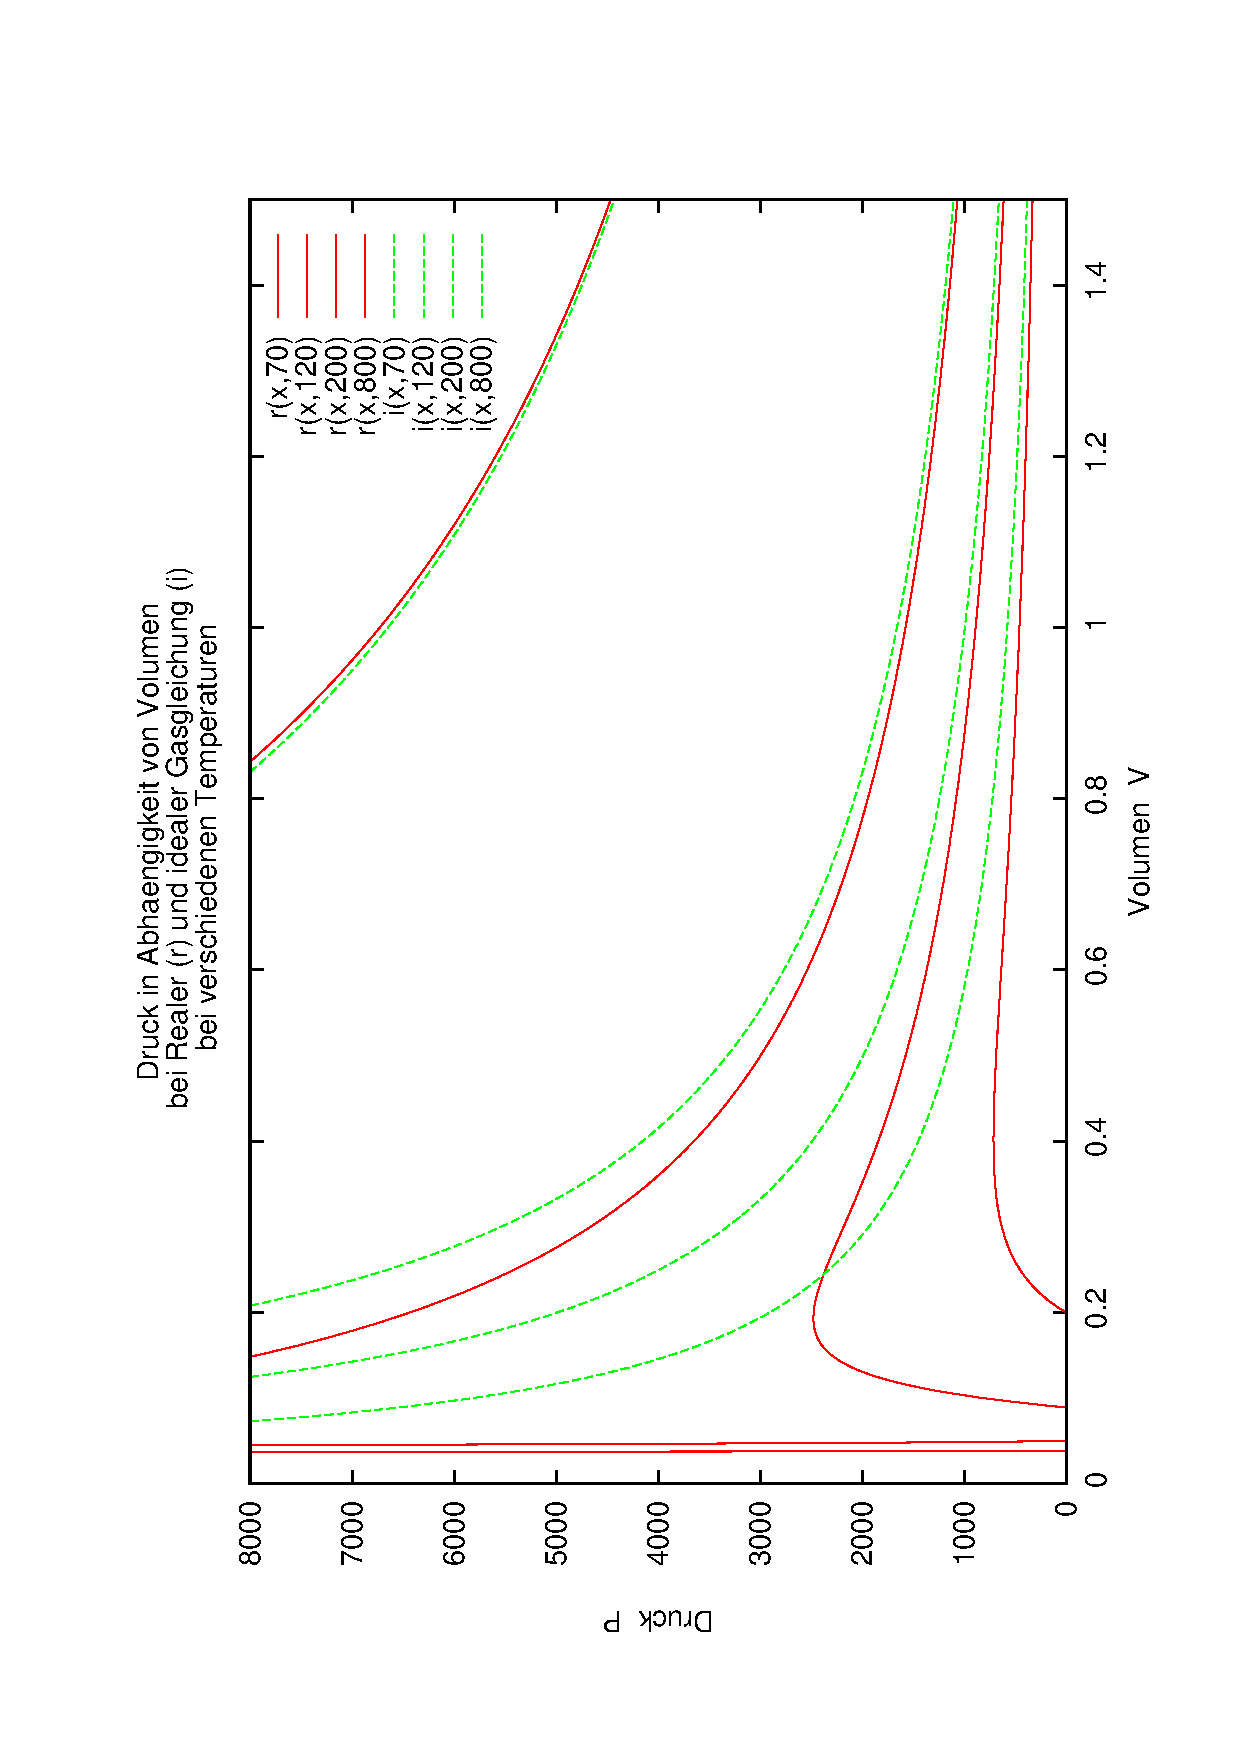
\includegraphics[width=0.7\textwidth,angle=-90]{bilder/real-ideal}}
   \subfigure[\label{abb_real_intressant}In einem interessanten
   Temperaturbereich kann man bei dem Kuververlauf des Realen Gases
   diverse Wendepunkte
   sehen]{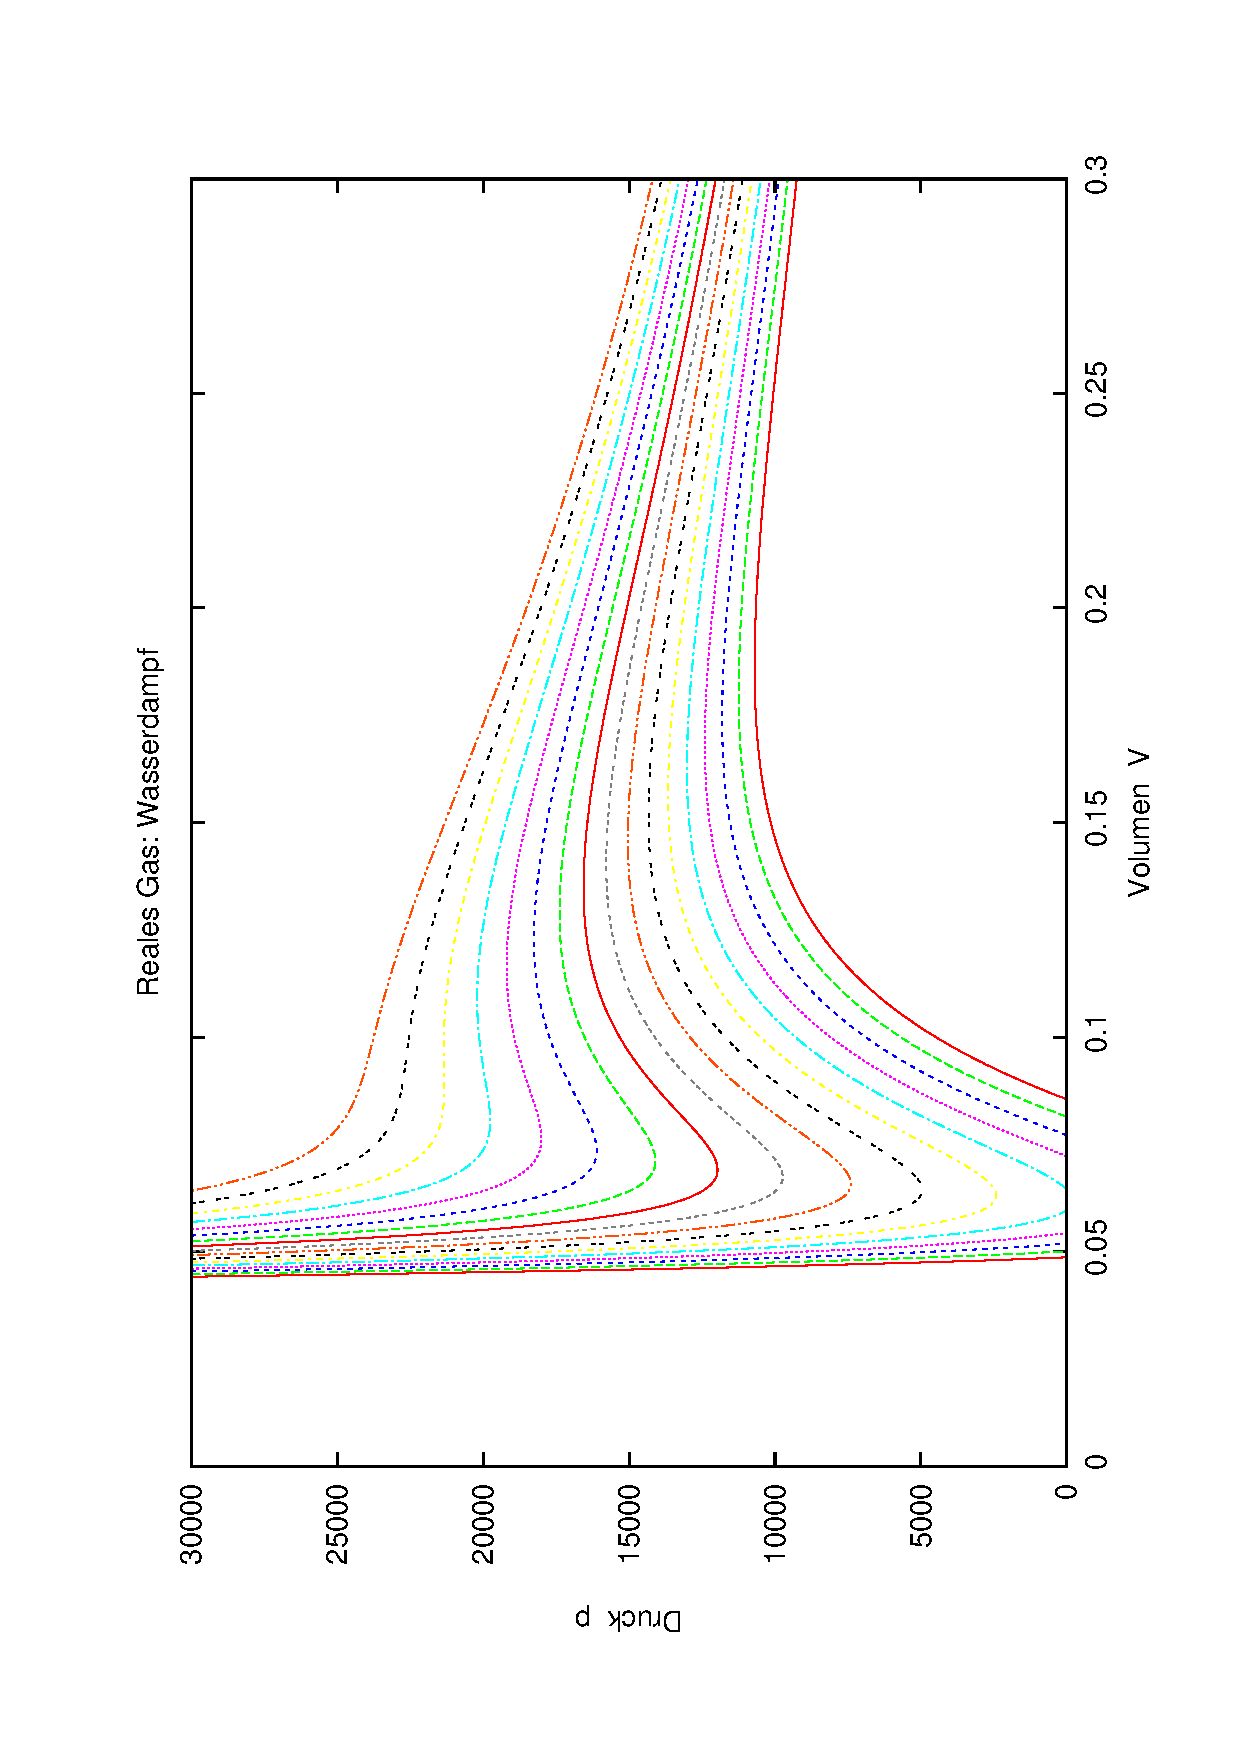
\includegraphics[width=0.7\textwidth,angle=-90]{bilder/real2}}
   \caption{Diagramme Idealer und Realer Gase}
   \label{abb_ideal-real_gas}
\end{figure}


\begin{Wichtig}
Der in Abb. \ref{abb_real_intressant} skizzierte
Verlauf tritt nur rechnerisch ein; in der Realit"at wird das nicht so
kommen:   
\end{Wichtig}
Die Wendepunkte verschwinden in der Praxis und stattdessen
werden die konkaven Abschnitte durch eine $x$-Achsen-Parallele
ersetzt, sodass die zwischen Gerade und Funktion eingeschlossenen
\emph{Orientierten Fl"achen}\footnote{also eine positive, wenn die
  Funktion gr"o"ser als die Gerade ist und eine negative, wenn die
  Funktion kleiner ist} in der Summe $0$ ergeben.
In Abb. \ref{abb_real-richtig} ist so etwas skizziert.

Die Temperatur, bei der sich gerade nur ein Wendepunkt bildet, wird
mit $T_k$ bezeichnet.\footnote{Entsprechend das entsprechende Volumen
  als $V_k$ und der dazugeh"orige Druck als $p_k$.} Wie in
Abb. \ref{abb_real-richtig} zu sehen ist, bildet sich eine Kurve, wenn
man die Punkte miteinander verbindet, die den Unterschied zwischen
Formel und Experiment markieren. Zusammen mit der Kurve mit nur einem
Wendepunkt (die also bei $T_k$ aufgenommen wurde) teilt sie das
Diagramm in Vier Abschnitte -- I bis IV -- auf:

\begin{description}[\setlabelstyle{\bfseries\slshape}]
\item[Bereich III] Das Volumen ist gro"s, der Druck jedoch klein; Das
   System bleibt \textbf{gasf"ormig}.
\item[Bereich II] Der Druck ist im Experiment konstant (deshalb die
   Konstruktion der Parallelen Linien), obwohl $V$ gr"o"ser oder kleiner
   wird.

   Die Gasteilchen kommen sich n"aher und n"aher und attraktive Kr"afte
   wirken zwischen ihnen. Manche der Gasteilchen kondensieren so und
   senken so den Druck weiter (weil die fl"ussigen Teilchen weniger
   Platz brauchen). Je weiter das Volumen reduziert wird, desto mehr
   Teilchen kondensieren, also desto mehr Fl"ussigkeit entsteht.

   Insgesamt liegt eine \textbf{Koexistenz} zwischen gasf"ormigem und
   fl"ussigem Zustand vor, die sich weiter in Richtung Fl"ussigkeit
   verschiebt, je kleiner das Volumen wird.

\item[Bereich I] Alles (oder zumindest viel Gas) ist kondensiert --
   schon f"ur geringe Volumen"anderungen ist ein sehr gro"ser Druck n"otig
   (Im Schaubild strebt die Druck-Kurve hier gegen $\infty$). Die
   Teilchen liegen also gr"o"stenteils als \textbf{Fl"ussigkeit} vor.


\item[Bereich IV] Hier befinden wir uns oberhalb der Temperatur $T_k$
   -- hier ist keine Kondensation m"oglich; die kinetisch Energie der
   Teilchen ist zu gro"s, als dass die zwischenmolekularen Kr"afte so
   stark wirken k"onnten, dass sich eine Fl"ussigkeit bildet.

Diesen Zustand nennt man \textbf{Fluid}.
\end{description}

\begin{Def} 
   [\label{def_fluid}\index{Fluid}Fluid] Ein Fluid ist eine
   Substanz, die man verformen kann, ohne dass sie einen Widerstand
   entgegen setzt. In diesem Sinne geh"oren zu den Fluiden sowohl Gase
   als auch Fl"ussigkeiten.
\end{Def}

Diese Verallgemeinerung macht Sinn, weil viele physikalische Gesetze
f"ur Gase und Fl"ussigkeiten (qualitativ) gleicherma"sen gelten und
die Eigenschaften sich nur quantitativ unterscheiden.

Mit anderen Worten: Es macht hier keinen Sinn, zwischen Fl"ussigkeit
und Gas zu unterscheiden, deshalb nenne man den Zustand Fluid.

In Tabelle \ref{tab_Tk} sind ein paar der kritischen Temperaturen
aufgef"uhrt, wie sie im Experiment vorkommen.

\bigskip
\noindent

So kann man auch noch ein
sog. \textbf{\index{Phasendiagramm}Phasendiagramm} zeichnen. In ihm
wird genau festgehalten, wie das \emph{Verh"altnis von Druck und
  Temperatur} sein muss, damit man eine bestimmte Phase erh"alt. In
Abb. \ref{abb_pasendiagramm} ist ein solches
dargestellt.\footnote{Bitte beachten: dies ist ein $p$-$T$-Diagramm;
  man kann es nur schwer mit den $p$-$V$-Diagrammen wie
  \ref{abb_ideal-real_vgl} oder \ref{abb_real-richtig} vergleichen!} 

Um die Kurve, welche den fl"ussigen vom gasf"ormigen Zustand eines Mols Gas
trennt (auch \emph{Siedekurve} genannt) zu berechnen, verwendet man
$$
p(T) = p_0 \cdot \exp \frac{-Q_D}{RT}
$$
wobei mit $Q_D$ die \emph{Verdampfungsw"arme} eines Mols der Teilchen ist.






\begin{figure}[h]
   \centering
   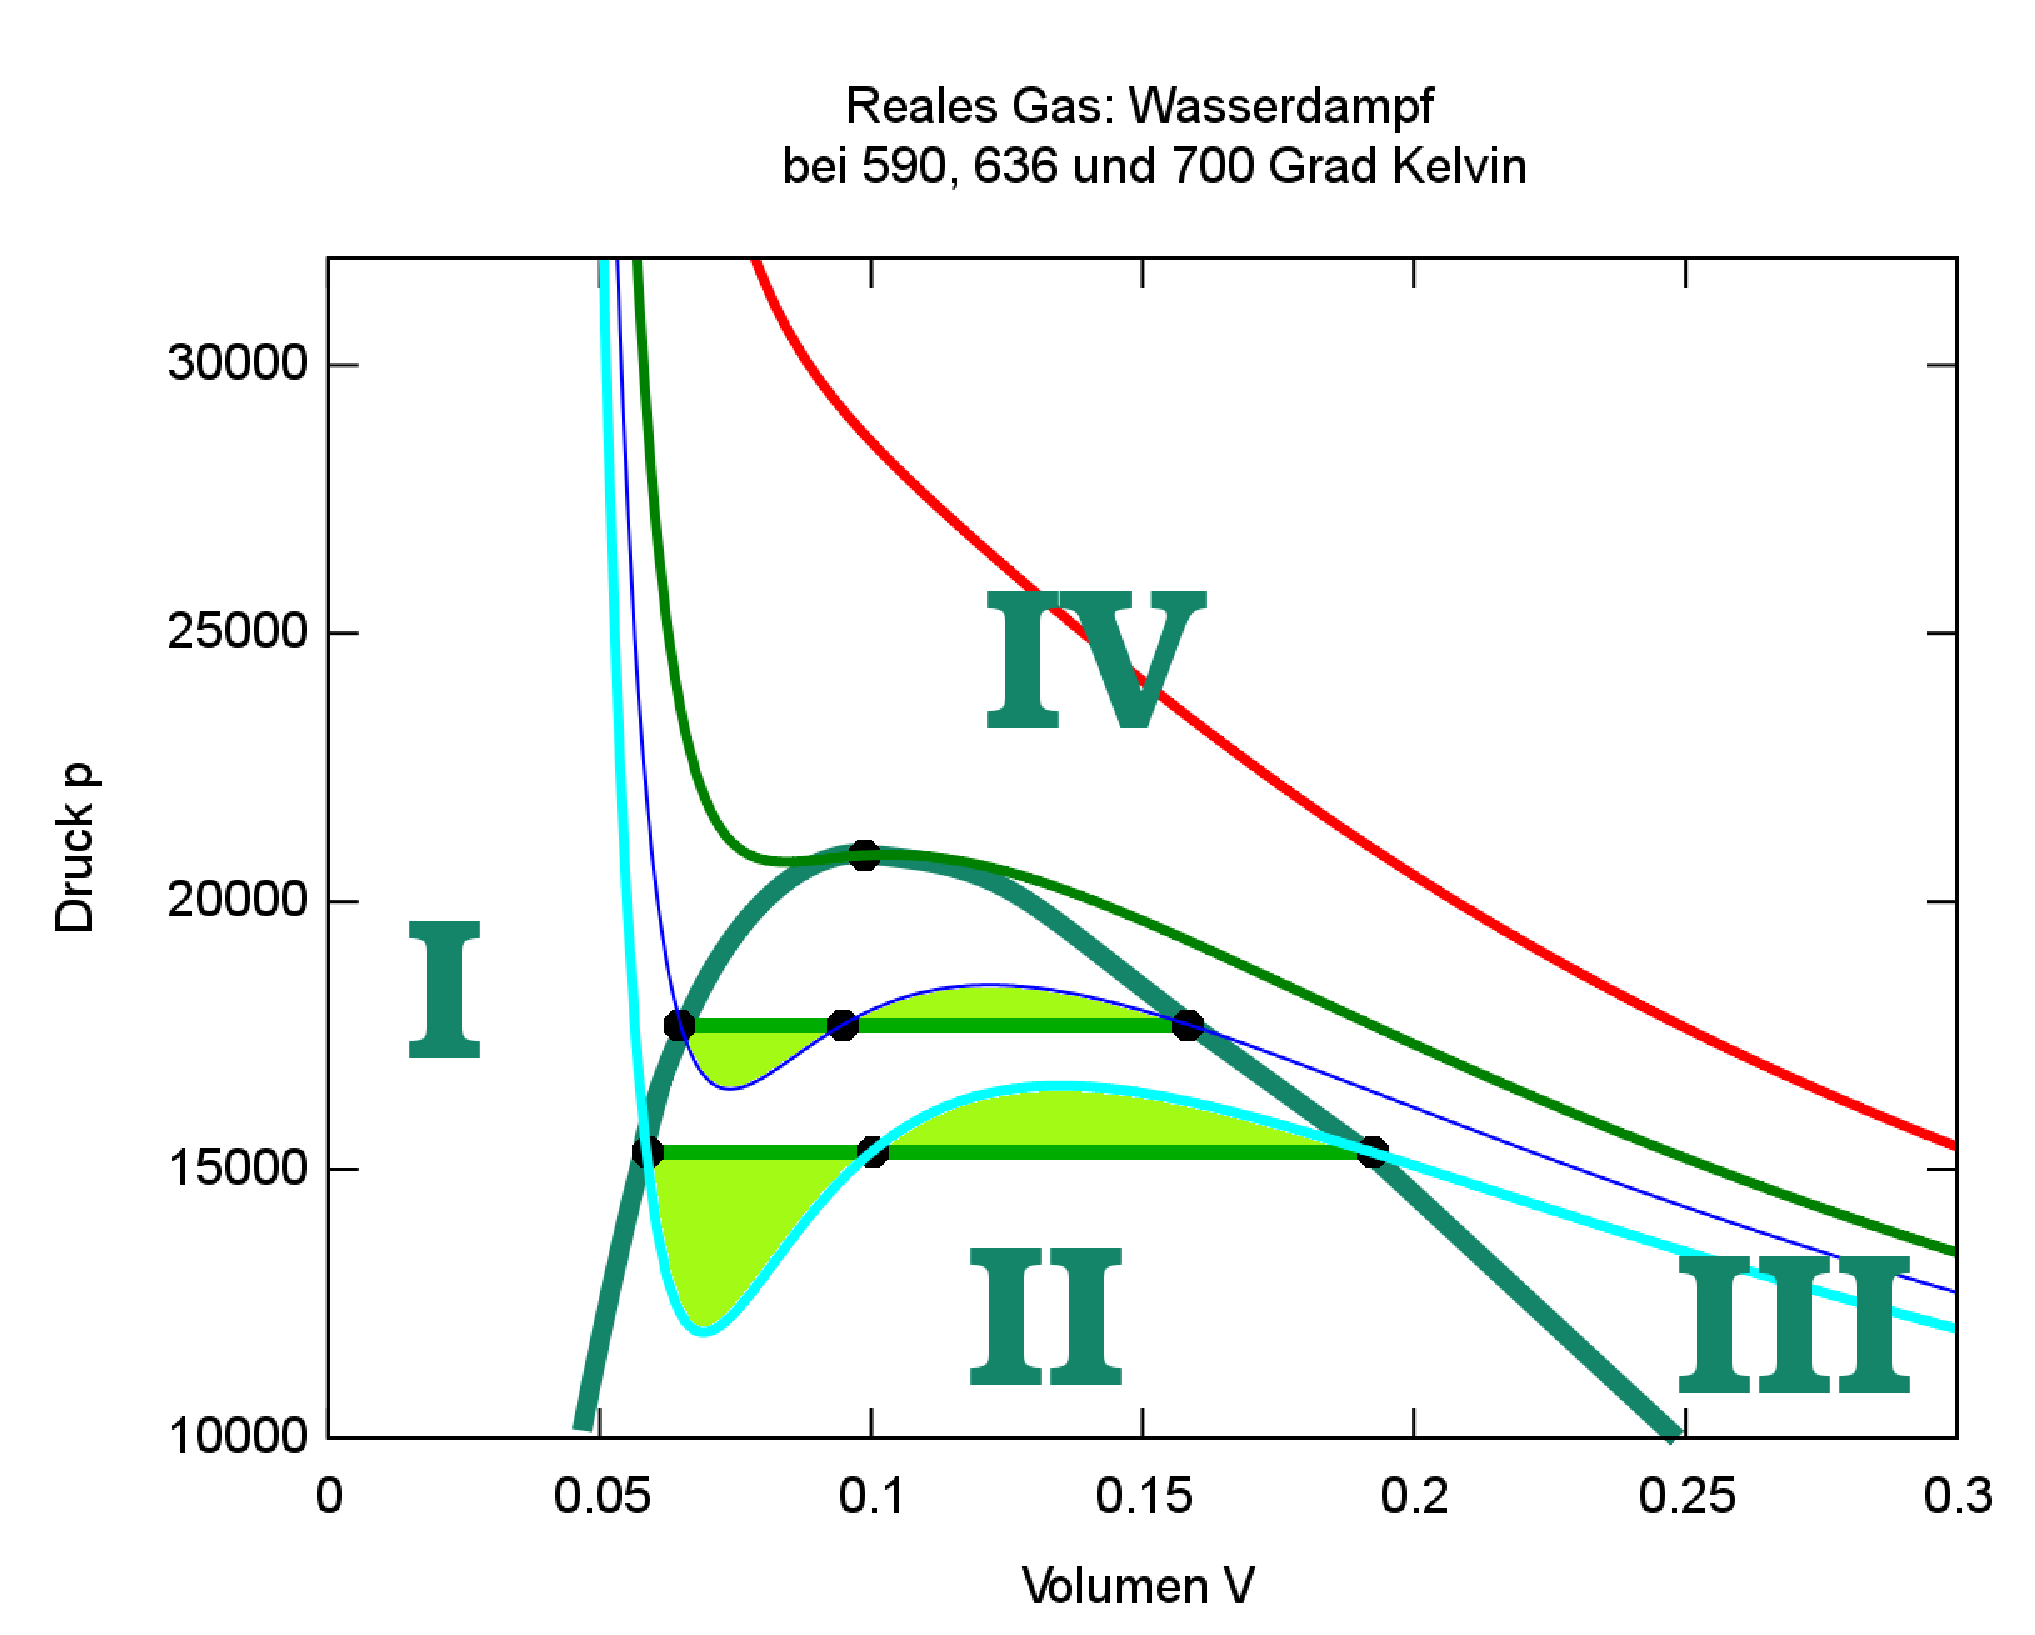
\includegraphics[width=12cm]{bilder/real2c_mod2}
   \caption[p-V-Diagramm reales Gas]{Realer Kurvenverlauf skizziert,
     mit diversen Konstruktionshilfen und den gebieten I bis IV
     eingezeichnet.}
   \label{abb_real-richtig}
\end{figure}



\begin{table}[h]
   \centering
   \begin{tabular}{l | r r r}
\toprule
      ~ & $\mathbf{p_k}$ in bar & $\mathbf{T_k}$ in K &
      $\mathbf{\varrho_k}$ in
      $\frac{\operatorname{kg}}{\operatorname{m}^3}$ \\
\midrule
      $H_2$ & 12,9 & 33,2 & 31\\
      $CO_2$ & 73,7 & 304,1 & 465 \\
      $H_2O$ & 221,0 & 647,3 & 317 \\
\bottomrule
   \end{tabular}
   \caption{Tabelle kritischer Dampfdr"ucke, Temperaturen und Dichten von Gasen}
   \label{tab_Tk}
\end{table}


\begin{figure}
   \centering
   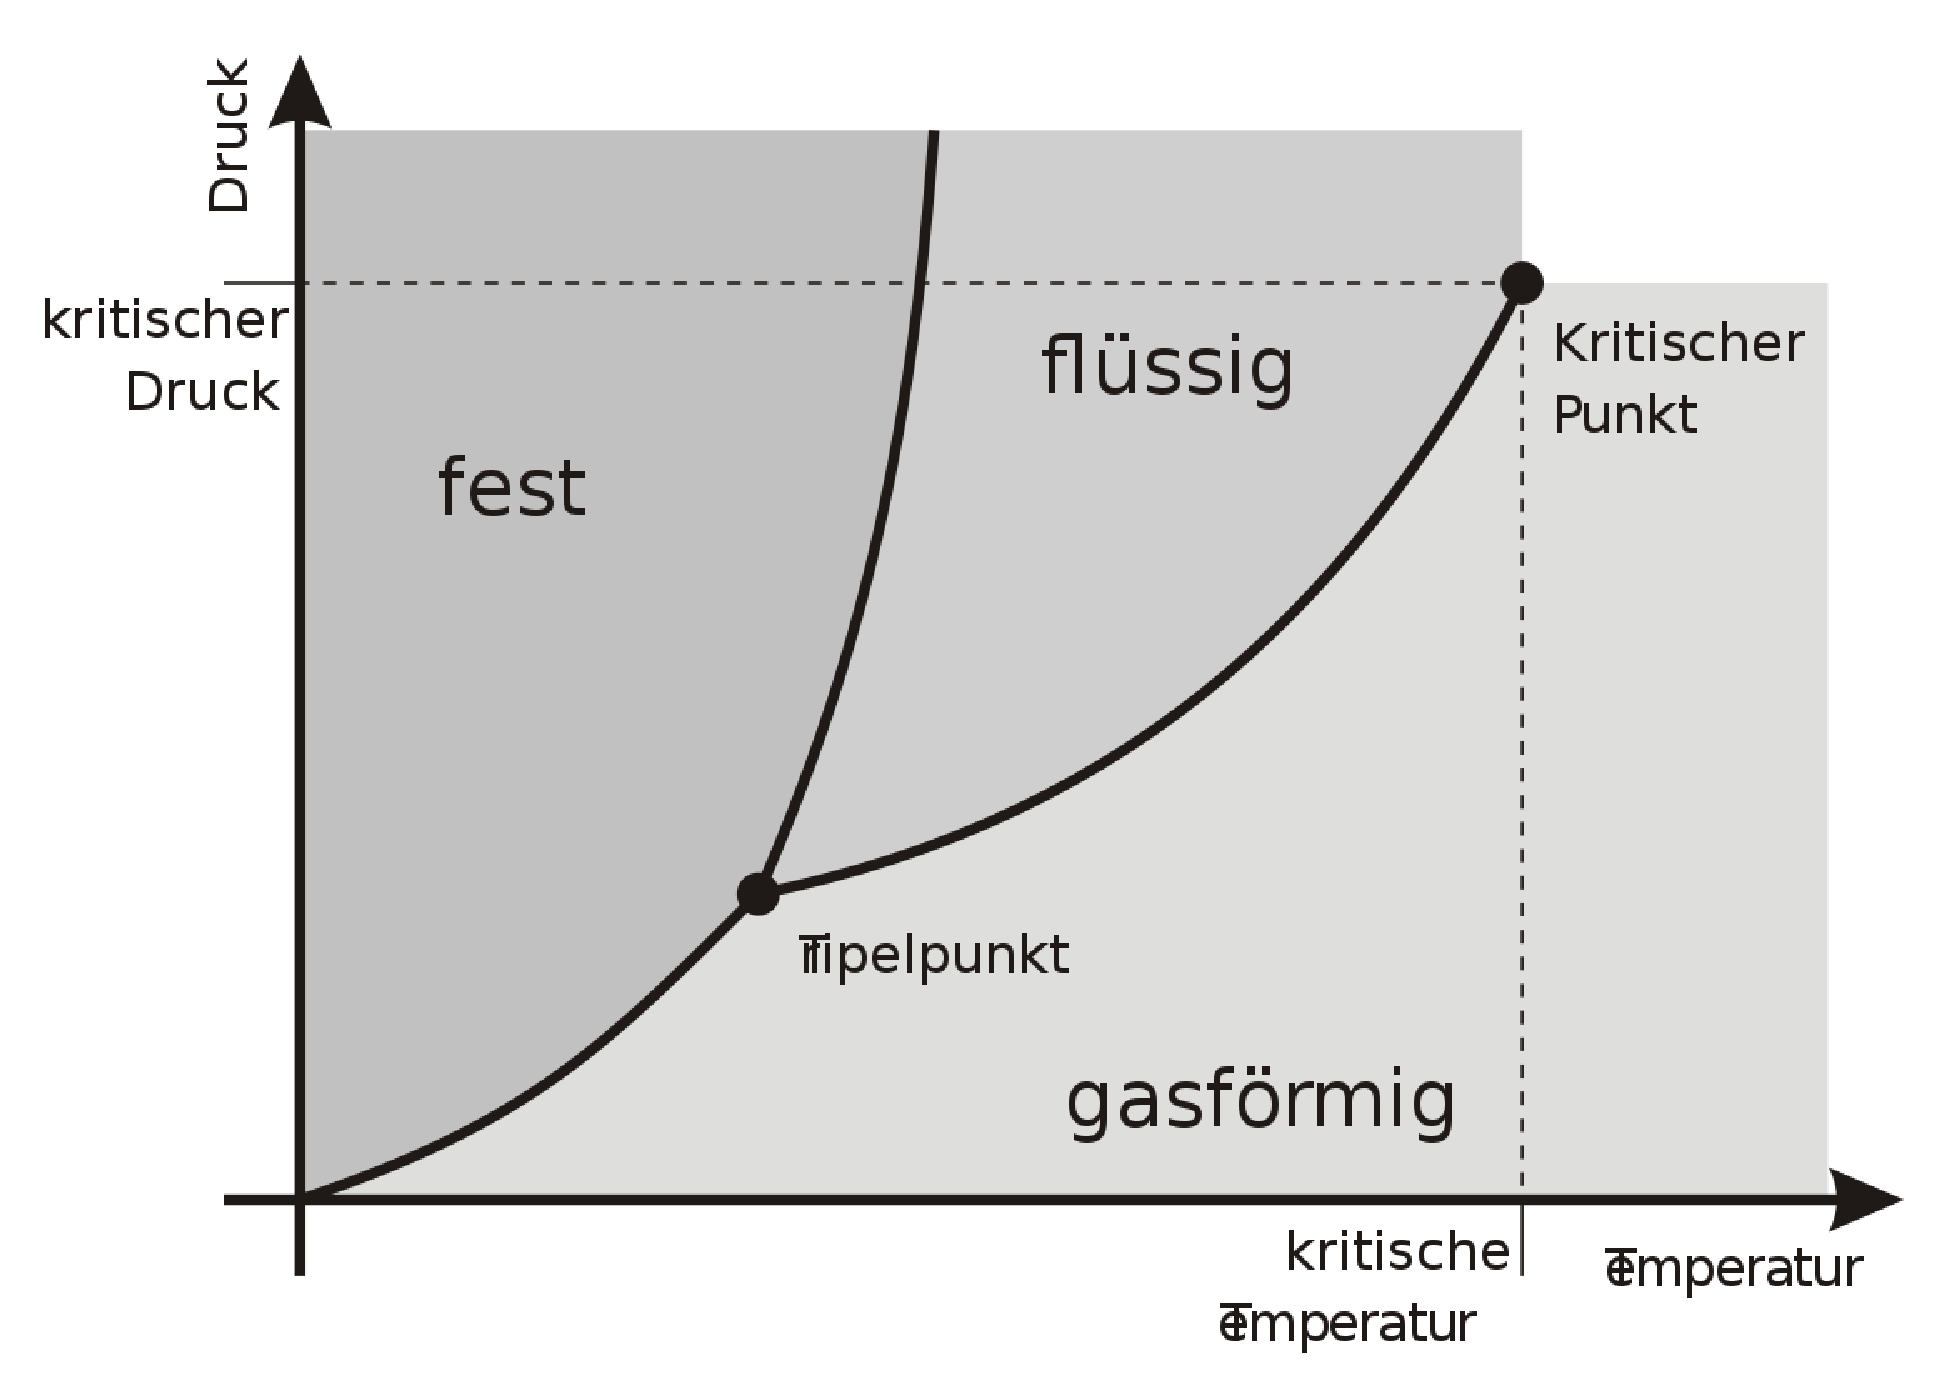
\includegraphics[width=0.6\textwidth]{bilder/phasen}
   \caption[Phasendiagramm: reales Gas]{Phasendiagramm eines realen Stoffes (ohne Anomalie -- also nicht wie
Wasser). (Quelle: \textsc{Wikipedia})}
   \label{abb_pasendiagramm}
\end{figure}




\clearpage

\section[\textsc{Guggenheim}-Quadrat]{Das \textsc{Guggenheim}-Quadrat (und seine Vergewaltigung) $(\bigstar)$}
\label{kap_guggenheim-quadrat-und-seine-vergewaltigung}



\begin{figure}
   \centering
   \includegraphics[width=0.6\textwidth]{bilder/guggenheim}
   \caption{Das \textsc{Guggenheim}-Schema}
   \label{abb_guggenheim}
\end{figure}


In Abb. \ref{abb_guggenheim} ist das \textsc{\index{Guggenheim
    Schema}Guggenheim}-Schema dargestellt. Es erm"oglicht, sich
zahlreiche Zusammenh"ange der Thermodynamischen Gr"o"sen (mit geringem
Aufwand) zu merken.

Darin stehen die Buchstaben f"ur: S: Entropie, V: Volumen, T:
Temperatur, p: Druck, H: Enthalpie, U: Innere Energie, F: Freie
Energie und G: Gibbs'sche Enthalpie. Um sich dieses Schema merken zu
k"onnen, gibt es einen sch"onen Merkspruch:
\begin{quote}
   \textbf{S}o \textbf{V}iel \textbf{T}hermo-\textbf{P}hysik
   \textbf{H}"atte \textbf{U}ns \textbf{F}ast \textbf{G}eschafft!
\end{quote}
Dabei f"angt man in der linken unteren Ecke an und schreibt im
Uhrzeigersinn die vier Zustandstr"o"sen S, V, T und p an und beginnt
direkt hinter p mit den restlichen Gr"o"sen. Die Pfeile haben
anschlie"send eine wichtige Bedeutung.

Es gelten nun folgende "`Gebrauchsanweisungen"':
\begin{description}[\setlabelstyle{\bfseries\slshape}]
\item[Ableitungen] Um Partielle Ableitungen der Gr"o"sen nacheinander zu
   gewinnen, gilt die Formel:
   \begin{equation}
      \label{eq:430}
      \left ( \frac{\partial <\text{Kante}>}{\partial <\text{Ecke}>} \right )_{<\text{Ecke
          des Dreiecks}>} = \pm <\text{Pfeil folgen}>
   \end{equation}
D.h. man W"ahlt eine Gr"o"se auf der Kante $X$ (bspw. $H$) und bewegt sich zu
einem anliegenden Eck $Y$ (bspw. $S$) um die partielle Ableitung
$\frac{\partial X}{\partial Y}$ zu bestimmen. Nun folgt man dem Pfeil
zur n"achsten Ecke und erh"alt hier die Gr"o"se $Z$ rechts der
Gleichung. Wenn man dabei \emph{mit} dem Pfeil gegangen ist, ist das
Vorzeichen \emph{positiv}, \emph{entgegen} dem Pfeil, ist es
\emph{negativ}. Bei der Ableitung hat eine Gr"o"se konstant zu bleiben:
Dabei handelt es sich um die Ecke $W$, welche zusammen mit den bisher
gew"ahlten Gr"o"sen ein rechtwinklig, gleichschenkliges Dreieck
bildet. Es ist dann:
\begin{equation*}
\left (   \frac{\partial X}{\partial Y} \right )_W = \pm Z
\end{equation*}
Und so bspw:
\begin{equation*}
   \left ( \frac{\partial H}{\partial S} \right )_p = T 
\text{ oder }
\left ( \frac{\partial H}{\partial p} \right )_S = V
\text{ oder }
\left ( \frac{\partial U}{\partial V} \right )_S = -p
\end{equation*}
F"ur diese Aufgabe ist das Schema eigentlich gemacht, deshalb stimmen
hier die Pfeilrichtungen mit $+$ und $-$ "uberein.
\item[Totale Differenziale] 
So kann man die totalen Differenziale einer der \textbf{Kanten}
bestimmen:
\begin{equation}
   \label{eq:431}
 \diff  <\text{K.}> = \pm <\text{E. gegen"uber}> \diff
 <\text{P. folg.}> \pm <\text{andere E.}> \diff <\text{P. folg.}>
\end{equation}
D.h. man w"ahlt eine Kante und geht von dieser zur gegen"uberliegenden
Ecke und mulipliziert diese Gr"o"se mit dem Differenzial der Gr"o"se, zu
der man gelangt, wenn man dem Pfeil folgt (in der endg"ultigen Formel
sind also die Gr"o"sen aller drei Differenziale Nachbarn im
\textsc{Guggenheim}-Quadrat). Das Vorzeichen ist dabei ist \emph{mit}
der Pfeilrichtung \emph{negativ} und \emph{entgegen} der Pfeilrichtung
positiv. Wichtig ist dabei, dass man \emph{beide} gegen"uberliegende
Ecken enbezieht, also im Endeffekt alle vier Zustandsgr"o"sen gebraucht
hat.

Bspw. gilt:
\begin{equation*}
   \diff H = T \diff S + V \diff p \text{ oder } \diff G = V \diff p -
   S \diff T
\end{equation*}
\item[\textsc{Maxwell}-Beziehungen] 
Hier kann man die Ecken gegeneinander partiell ableiten. Es gilt:
\begin{equation}
   \label{eq:432}
   \left ( \frac{\partial <\text{E.1}>}{\partial <\text{E.2}>} \right
   )_{<\text{Nenner gegen"ub.}>} = \left ( \frac{\partial
        <\text{P. folgen}>}{\partial <\text{letze E.}>} \right
   )_{<\text{Nenner gegen"ub.}>}
\end{equation}
Dabei w"ahlt man die ersten beiden Ecken frei aus und bildet die linke
Ableitung.  Dann folgt
man dem Pfeil (von $<\text{E.2}>$) zur n"achsten Ecke und bildet mit
dieser und der letzten Ecke die rechte Ableitung. Dabei ist bei der
linken Ableitung die Gr"o"se Konstant, die Rechts im Nenner steht und
anderst herum.  Auf einer der Seiten \emph{sowohl} $S$ als auch $p$
auftauchen (diese liegen beide an den stumpfen Pfeilenden), dann kommt
vor diese Ableitung ein "`$-$"', sonst \emph{nicht}.

Also bspw.:
\begin{equation*}
   \left ( \frac{\partial V}{\partial T} \right )_p = - \left (
      \frac{\partial S}{\partial p} \right )_T
\text{ oder }
\left ( \frac{\partial T}{\partial p} \right )_S = \left ( \frac{\partial V}{\partial S} \right )_p
\end{equation*}

\item[Definitionen] 
Man kann die drei Definitionen 
\begin{eqnarray*}
   \mathcal F &=& U - TS ~  \text{ eigentlich } U = \mathcal F + TS\\
G &=& H - TS \\
H &=& U + pV
\end{eqnarray*}
(mit ein wenig Gewalt) in das Schema pressen:
\begin{equation}
   \label{eq:433}
<\text{K.}> = <\text{n"achste K.}> \pm <\text{n"achste E.}> \cdot
<\text{P. folgen}>
\end{equation}
% Man w"ahlt also eine Kante und bewegt sich zur n"achsten Kante. Die
% "`n"achste"' ist im Falle von $G$ und $H$ im Uhrzeigensinn und bei
% $\mathcal F$ im \emph{Gegen}uhrzeigersinn.
Man w"ahlt also eine Kante und bewegt sich zur n"achsten Kante im
Uhrzeigersinn, weiter zur n"achsten Ecke und folgt hier dem Pfeil.
Das Vorzeichen ist wieder positive, wenn man \emph{gegen} den Pfeil
geht und \emph{mit} dem Pfeil \emph{negativ}.
\end{description}

\abs
Man kann diese Relationen herleiten, indem man bekannte Gr"o"sen per
\textbf{Legendre}-Transformation transformiert (damit kann man elegant
die totalen Differenziale umschreiben) und erh"alt durch
Koeffizientenvergleiche die Ableitungen $\frac{\partial
  <\text{Kante}>}{\partial <\text{Ecke}>}$.

Mit diesen Grundgleichungen zusammen mit $\bar u = \frac{f}{2} K_B T$
kann man viele der hier besprochenen F"alle schnell und einfach nachrechnen!






















 \chapter{Mikroskopische Thermodynamik}
\label{kap_mikroskopische-thermodynamik}




In diesem Kapitel betrachten wir einzelne Atome, Molek"ule oder einfach
kleinste Teilchen -- jedoch versuchen war gar nicht erst, f"ur die
gro"sen Mengen an Teilchen exakte Bewegungsgleichunge zu l"osen, sondern
verwenden die Aussagen aus der Thermodynamik (Kap
\ref{kap_thermodynamik}), die wir aus Beobachtungen des Makrozustandes
gewonnen haben, und untersuchen damit das Verhalten der kleinsten
Teilchen.

Wir verlassen uns also auf \emph{statistische} Ans"atze, die uns zwar
keine exakten Aussagen erm"oglichen, daf"ur aber eine Aussage, die
f"ur ein Teilchen \emph{im Allgemeinen} gilt. Eine wohldefinierte,
konstante (makroskopische) Zustandsgr"o"se ist auf der mikroskopischen
Scala unter Umst"anden starken Schwankungen unterworfen -- so als
w"urden wir unsere Messergebnisse jetzt unter dem Mikroskop
betrachten.

Wie im \textsc{Feynmann}'schen Experiment der \textbf{Molekularen
  Ratsche} kann es dabei zu eigentlich verwirrenden Ergebnissen kommen
-- die sich aber doch wieder logisch "uber bekannte physikalische
Probleme erkl"aren lassen.






\section{\textsc{Stokes-Einstein}-Relationen}
\label{kap_stokes-einstein-relationen}

Wir betrachten $N$ \index{Kolloid}Kolloide\footnote{Kleine
  Teilchen ($d \approx 1 \operatorname{\mu m}$) die jedoch noch
  \emph{weit gr"o"ser} sind, als die Teilchen der L"osung. Eine
  \emph{kolloidale L"osung} kann bspw. ein klares L"osungsmittel sein,
  in dem so viele Kolloide das Licht streuen, dass die Fl"ussigkeit
  eine milchige Tr"ubung erh"alt.}, die in einem Fl"ussigkeitsvolumen
$V$ \index{Suspension}suspendiert\footnote{Ein Feststoff ist in einer
  Fl"ussigkeit fein verteilt, aber immer noch im festen
  Aggregatszustand.} sind und definieren die \textbf{Teilchendichte}:
\begin{equation}
   \label{eqn_def_teilchendichte}
   n_K = \frac{N}{V} = \frac{p}{K_B T}
\end{equation}
Sei nun $n_K$ hinreichend klein -- also wenige dieser Kolloide
"`gel"ost"', so kann man die Kolloide als Ideales Gas behandeln (und
die Fl"ussigkeit als Vakuum zwischen den "`Gasteilchen"').


\subsection{Betrachtung als Kr"aftegleichgewicht}
\label{kap_betrachtung-als-kraftegleichgewicht}


Die "`Gasteilchen"' respektive Kolloide erzeugen den Druck
\begin{equation}
   \label{eq:13}
   p = n_K \cdot K_B \cdot T
\end{equation}
%
%\abs
Auf die Kolloide wirkt noch eine weiter Kraft $F$ --
bspw. \emph{Graviatation}, ein \emph{elektrisches Feld} etc. Im
Thermischen \emph{Gleichgewicht} gilt:
$$
 \sum_i F_i = 0
$$
und so f"ur die \emph{\index{Kraftdichte}Kraftdichten} 
\begin{Def}
   [Kraftdichte $\vec f$] Die Kraftdichte $\vec f$ ist als "`Kraft pro
   Volumen"' so definiert, dass 
   \begin{equation}
      \label{eq:210}
\diff \vec F = \vec f \diff V ~ \text{ oder } ~ \vec F = \int_V \vec f \diff V
   \end{equation}
 ist.
\end{Def}
Die Kraftdichte ergibt sich aus dem Druck durch
\begin{equation}
   \label{eq:208}
   \vec f = \vec f(\vec r) = - \vec \nabla p(\vec r)
\end{equation}
Wenn die Kr"afte auf alle $N$ Teilchen der Teilchendichte $n = \frac{N}{V}$ gleich
wirken  und auf jedes Teilchen  die Kraft $\vec F$ wirkt, so folgt f"ur die
Kraftdichte und weil insgesamt die Kraft $N\, \vec F$ wirkt:
\begin{equation*}
\vec f = \frac{N \, \vec F}{V} = \vec F \cdot n
\end{equation*}
Damit und der Definition aus Gl. \eqref{eq:210} folgt so:

\begin{equation}
   \label{eq:14}
   n_K(\vec r) \cdot \vec F + \Vec \nabla p(\vec r) = 0
\end{equation}
mit Gl. \eqref{eq:13} folgt
\begin{equation}
   \label{eq:15}
   \frac{p(\vec r)}{K_B T} \cdot \vec F + \vec \nabla p(\vec r) = 0
\end{equation}
Dies ist eine (partielle) Differentialgleichung mit der L"osung
\begin{equation}
   \label{eq:16}
   p(\vec r) = \underbrace{\exp \left ( - \frac{\vec F \cdot \vec
          r}{K_B T} \right )}_\text{ \textsc{Boltzmann}-Faktor } ~ \sim
   ~ n_K(\vec r)
\end{equation}
Die Proportionalit"at zu $n_K$ ergibt sich aus Gl. \eqref{eq:13}. Dies
ist eine
\emph{\textsc{\index{Boltzmann-Verteilung}Boltzmann}-Verteilung}!

\abs
Nun k"onnen wir als Spezialfall die \textbf{Gravitation} als Kraft
verwenden mit $\vec F = m \cdot \vec g$:
\begin{equation}
   \label{eqn_barometrische-hoehenformel-thermo}
   n_K(h) \sim 
\exp \left ( - \frac{mg \cdot h}{K_B T} \right )
\end{equation}
und erhalten die \textbf{\index{Barometrische H"ohenformel}Barometrische
H"ohengleichung}; die Kolloide
in der L"osung verhalten sich also wie die Luft in der Atmosph"are.




\subsection{Betrachtung mit Teilchenstrom}
\label{kap_betrachtung-mit-teilchenstrom}

Der Gleichgewichtszustand des Systems ist Ergebnis zweier
gegenl"aufiger Teilchenstr"ome.

\begin{Def}
   [\index{Teilchenstrom}Teilchenstrom $\vec j$]
gibt an, wie sich die Teilchen\emph{dichte} ausbreitet (nicht
ein einzelnes Teilchen).
Es gilt
\begin{equation}
   \label{eqn_def_teilchenstrom}
   \vec j = n_K(\vec r) \cdot \vec v ( \vec r )
\end{equation}
\end{Def}

Bei uns laufen gegeneinander
\begin{enumerate}
\item \index{Diffusionsstrom}Diffusionsstrom\\Teilchen str"omen nach oben, weil oben im Gef"a"s
   die Dichte kleiner ist. Die Diffusion l"auft entgegen des
   Gradienten\footnote{weil der Gradient ja in die Richtung der
     \emph{gr"o"sten} "Anderung zeigt, also dorthin, wo die Dichte weiter
   zunimmt}:
   \begin{equation}
      \label{eqn_diffusionsstrom}
      \vec j_\text{dif} =  - D \cdot  \nabla n_K(h)
   \end{equation}
   Dabei ist $D$ der
   \emph{\index{Diffusionskoeffizient}Diffusionskoeffizient} (mit $[D]
   = \frac{m^2}{s}$).

   Nur mit der Diffusion w"urden die Teilchen sich lediglich
   gleichverteilen.

\item Driftstrom\\Durch die Schwerkraft str"omen Teilchen nach
   unten. Mit der \textsc{Stokes}-Reibung 
$$
\vec F = 6 \pi \eta r \vec v
$$
mit der Viskosit"at $\eta$ und dem Teilchenradius $r$ ergibt sich (im
Gleichgewicht):
\begin{equation}
   \label{eqn_driftstrom}
   \vec j_\text{drift} = n_K \cdot \vec v = n_K \cdot \frac{\vec
     F}{6\pi\eta r}
\end{equation}
\end{enumerate}
Im Gleichgewicht gilt nun:
$$
\vec j_\text{dif} + \vec j_\text{drift} = 0
$$
und mit Gl. \eqref{eqn_diffusionsstrom} und \eqref{eqn_driftstrom}
gilt:
\begin{equation}
   \label{eq:10}
 D \cdot  \nabla n_K(h) =   n_K \cdot \frac{\vec
     F}{6\pi\eta r}
\end{equation}
Setzt man auf der linken Seite f"ur $n_K(h)$
Gl. \eqref{eqn_barometrische-hoehenformel-thermo} ein gilt mit 
$$
\nabla n_K(\vec h) = \nabla \exp \left ( - \frac{m\, \vec g \cdot \vec
     h}{K_B T} \right ) = - \frac{m\, \vec g}{K_B T} \cdot \exp \left ( -
   \frac{m\vec g \cdot \vec h}{K_B T} \right ) = - \frac{\vec F_g}{K_B
  T} \cdot n_K(\vec h)
$$
und da $\vec F = -\vec F_g$ gilt f"ur Gl. \eqref{eq:10}:
\begin{equation*}
   \label{eq:17}
   D \cdot \frac{\vec F}{K_B T} \cdot n_K(h) =  n_K \cdot \frac{\vec
     F}{6\pi\eta r}
\end{equation*}
und so aufgel"ost nach $D$ ergibt sich die
\textbf{\textsc{Stokes-Einstein}-Relation}:
\begin{equation}
   \label{eqn_stokes-einstein-relation}
   \boxed{   
     D = \frac{K_B T}{6\pi\eta r} 
   }
\end{equation}


An dieser ist interessant, dass sie -- ganz im Geiste der
Mikroskopischen Thermodynamik -- die makroskopische Gr"o"se $D$ in
Zusammanhang bringt mit den atomaren Gr"o"sen $\eta$ und $r$.






\subsection{Mittlere Freie Wegl"ange}
\label{kap_mittlere-freie-weglange}

\begin{Def}
   [\index{Mittlere Freie Wegl"ange}Mittlere Freie Wegl"ange $\lambda$
   oder $\ell$] L"ange $\lambda$, wie weit sich ein Teilchen bewegn
   kann, ohne mit einem anderen zu kollidieren.
\end{Def}

\begin{Wichtig}
   Der mittlere Teilchenabstand $\bar a$ ist verschieden von der
   mittleren freien Wegl"ange $\lambda$.
\end{Wichtig}

Wir unterteilen das Volumen $V$, welches $N$ Teilchen enth"alt, nun in
$N$ W"urfel mit der Kantenl"ange $a$; und
% $$
% V = N \cdot a^3
% $$
mit \eqref{eqn_def_teilchendichte} folgt
\begin{equation}
\label{eq:18}
   V = Na^3 = \frac{N}{n_K} ~ \Rightarrow ~ \frac{1}{n_K} = a^3
~ \Rightarrow ~
\sqrt[3]{\frac{1}{n_K}} = n_K^{-\frac{1}{3}}= a 
\end{equation}
Es ist nun $a = \bar a \neq \lambda$: Denken wir uns die Gasteilchen
gleichverteilt -- mit Verteilung $n_K$ -- so hat jedes f"ur sich einen
eigenen kleinen W"urfel mit Kantenl"ange $a$. Denken wir nun, dass
jedes Teilchen sich nur in seinem W"urfel bewegt, so haben sie im
Mittel den Abstand $\bar a$ voneinander.

\bigskip Wir betrachten nun einen Quader mit L"ange $\diff x$ und
Seitenfl"ache $A$, in dem sich $N$ Teilchen (mit Dichte $n_K$) befinden
und sich bewegen. Von au"sen fliegt ein weiteres Teilchen auf $A$
zu. Man projeziert nun die Teilchen \emph{im} Quader parallel zur
Bewegung $\vec v$ des anfliegenden Teilchens auf die Fl"ache $A$. Ein
Teilchen mit Radius $r$ nimmt hier die Fl"ache 
\begin{equation}
   \label{eq:18b} 
   \sigma = \pi r^2
\end{equation}
ein -- die $N$ Teilchen logischerweise die Fl"ache $N \cdot \sigma$.

Die Wahrscheinlichkeit, dass das anfliegende Teilchen in der Zeit
$\diff t$ ein Teilchen im Quader erwischt ist
\begin{equation}
   \label{eq:19}
   \frac{A_\text{Teilchen}}{A_\text{Fl"ache insgesamt}} =
   \frac{\overbrace{n \cdot \overbrace{A \cdot \diff x}^V}^N \cdot
     \sigma}{A}
= n \cdot \sigma \cdot \diff x
\end{equation}
Aufgrund von Kollisionen nimmt die Zahl $j$ von Teilchen in $V$, die sich in
Richtung $\vec v$ bewegen (und so mit dem anfliegenden sto"sen), immer
weiter ab, je weiter man sich in $V$ hereinbewegt:
\begin{equation}
   \label{eqn_differenz-c0}
   j(x + \diff x) = j(x) - j(x) \cdot n \sigma \diff x
\end{equation}
(wir subtrahieren auf dem Weg nach $x$ von den sto"sbereiten Teilchen
$j$ die Teilchen, mit denen das anfliegende zusammenprallen wird ($j
\cdot n\sigma \diff x$, weil nach \eqref{eq:19} dies angibt, mit wie
vielen Teilchen aller
\emph{Wahrscheinlichkeit} nach das anfliegende sto"sen wird). 

Subtrahiren wir in \eqref{eqn_differenz-c0} $j(x)$ und teilen durch $\diff x$, so
haben wir eine Differentialgleichung. Eine L"osung ist
\begin{equation}
   \label{eqn_differenz-c1}
   j(x) = j_0 \cdot \exp ( - n \sigma x )
\end{equation}
Wir interpretieren das Ergebnis jetzt als \emph{Verteilung}: Je gr"o"ser
der Abstand $x$ wird, desto geringer ist die Wahrscheinlichkeit, dass
das Teilchen noch mit einem anderen st"o"st -- aber daf"ur ist die
Wahrscheinlichkeit, dass das Teilchen schon sehr fr"uh st"o"st,
au"serordentlich hoch, d.h. nur wenige Teilchen kommen "uberhaupt in die
N"ahe der gro"sen $x$. \eqref{eqn_differenz-c1} ist also die Verteilung der
Teilchen mit denen dein anfliegendes sto"sen kann, wobei $x$ dann
logischerweise f"ur die Strecke \emph{vor} dem Sto"s -- also die freie
Wegl"ange $\lambda$ -- steht.

Um jetzt noch die \emph{mittlere} freie Wegl"ange zu bestimmen,
verwenden wir eine Eigenschaft der $e$-Funktion: Das Mittel liegt bei
$y = \frac{1}{e}$; in unserem Fall also bei $\frac{1}{e} \cdot
j_0$. Mit $x = \lambda$ gilt:
\begin{equation}
   \label{eqn_differenz-c2}
   \boxed{
\lambda = \frac{1}{n \cdot \sigma}
}
\end{equation}



\subsection{Alternative Herleitung und Wirkungsquerschnitt $(\bigstar)$}
\label{kap_altern-herl-und-wirk-bigst}


In der vorhergehenden -- etwas weitschweifigen -- Herleitung haben wir
quasi nebenher bestimmt, mit welcher Wahrscheinlichkeit ein Teilchen,
welches sich um $x$ bewegt, st"o"st (Gl. \eqref{eqn_differenz-c1}).

Eine wesentlich \textbf{einfachere Herleitung} f"ur die mittlere freie
Wegl"ange $\lambda$ geht folgenderma"sen vor: Ein Teilchen habe wieder
die (effektive) Fl"ache $\sigma$ zu seiner
Bewegungsrichtung\footnote{Also die Projektion parallel der
  Bewegungsrichtung auf eine Fl"ache senkrecht zur Bewegungsrichtung
  ist $\sigma$.}. Wenn dieses Teilchen sich im Volumen $V$ mit
insgesamt $N$ Teilchen bewegt, so wird es \emph{im Mittel} (so ist ja
$\lambda$ definiert) die Strecke $\lambda$ zur"ucklegen k"onnen, ohne
gegen ein anderes Teilchen zu sto"sen. Dabei "uberstreicht es das
Volumen
\begin{equation*}
   V_{\lambda} = \sigma \cdot \lambda
\end{equation*}
Nun hat jedes Teilchen das selbe Volumen zur Verf"ugung -- also bei $N$
Teilchen folgt so -- wesentlich schneller --
\begin{equation}
   \label{eq:204}
   V_\lambda = \frac{V}{N} = \frac{1}{n} \equiv \sigma \cdot \lambda
   \text{ oder } ~ \lambda = \frac{1}{n \cdot \sigma}
\end{equation}


\abs Der \emph{Hintergrund} ist, dass in dieser kurzen Herleitung
$\sigma$ einfach als Querschnittsf"ache interpretiert wurde, in der in
der ersten Herleitung dagegen als
\textbf{\index{Wirkungsquerschnitt}Wirkungsquerschnitt}. Dieser ist
definiert als Ma"s f"ur die Wahrscheinlichkeit, dass ein bestimmter
Wechselwirkungsprozess (in unserem Falle ein Sto"s) zwischen Teilchen
eines Teilchenstrahls und einem Streuzentrum (hier die anderen
Teilchen) eintritt. Dieses Ma"s ist der Quotient aus gestreuten
Teilchen zum Teilchenfluss:
\begin{equation*}
   \sigma = \frac{\text{Gestreute Teilchen pro
       Zeit}}{\text{Anfliegende Teilchen pro Zeit und Fl"ache}}
\end{equation*}
und hat damit die \emph{Dimension} einer Fl"ache.

Alternativ kann man die anfliegenden Teilchen auch als Punktf"ormig
interpretieren. Dann stellt $\sigma$ eine Fl"ache auf dem Ziel
senkrecht zur Bewegungsrichtung des anfliegenden Teilchens dar, wobei
die Wechselwirkung stattfindet, wenn das Punktteilchen in $\sigma$
trifft und ausbleibt, wenn es an $\sigma$ vorbeigeht. Damit ist
$\sigma$ auch ein Ma"s f"ur die "`St"arke"' der Wechselwirkung. 

Die Wahrscheinlichkeit $w$ f"ur eine Wechselwirkung ergibt sich bei
einer Targetfl"ache von $A_T$ und $N_T$ Targetteilchen zu
\begin{equation*}
   w = \frac{\sigma \, N_T}{A_T} = \frac{N_W}{N} \text{ und damit } 
 \frac{\sigma}{A_T} = \frac{\frac{N_W}{N}}{N_T} = \frac{w}{N_T}
\end{equation*}
Hier bezeichnet $N_W$ die (angeflogenen) Teilchen, die gewechselwirkt
haben und $N$ die insgesamt angeflogenen Teilchen. 

Betrachten wir nun ein (d"unnes) Teilchenvolumen $V_T = A_T \cdot \diff
x$, so ist die Wahrscheinlichkeit f"ur einen Sto"s hier
\begin{equation*}
   w = \frac{N_W}{N} = \frac{\sigma \, N_T \cdot \diff x}{A_T \cdot \diff x}
=
\frac{\sigma \, \diff x \cdot N_T}{V_T} = \sigma \, n_T \, \diff x
\end{equation*}
wobei wir mit $n_T$ die \emph{Teilchendichte} der Zielteilchen
bezeichnen.  Bei dem Durchfliegen von $\diff x$ "`verliert"' man also
$w \cdot N$ Teilchen und hat so (wenn $N_0$ die anf"angliche
Teilchezahl im Teilchenstrahl war) $N_0 - N_W$ Teilchen "ubrig; damit
ist $N_W = - \Delta N$. Bei infinitissimaler Betrachtung f"uhrt das zu
\begin{equation*}
   - \diff N = N \cdot w = N \cdot \sigma n_T \, \diff x
\end{equation*}
und die L"osung dieser DGL (durch $N$ teilen und aufintegrieren) ist
\begin{equation*}
   N = N(x) = N_0 \E^{- \sigma n_T \, x} 
\end{equation*}
Wir betrachten nun, wann der Strahl auf $\frac{1}{\E}$ seiner
urpsr"unglichen Indensit"at abgesunken ist\footnote{Diese Betrachtung
  ist "ublich: Bei radioaktivem Zerfall betrachtet man die Zeit $\tau$,
zu der $\frac{1}{\E}$ des Urspr"unglichen Materials "ubrig ist, anstatt
der \emph{Halbwertszeit} $T_{1/2}$.}, also wenn $N(x) = \frac{1}{\E}\, N_0$.
Ein einfacher Koeffizientenvergleich liefert dann
\begin{equation*}
   \sigma n_T \, x = 1 ~  \text{ oder }  ~ \lambda = \frac{1}{n_T \, \sigma}
\end{equation*}
und danach definiert man die \emph{mittlere Freie Wegl"ange} $x \equiv \lambda$,
die diese Gleichung l"ost.

% Bewegen sich die Teilchen also $L$ in das Target hinein, sind $N(L)$
% Teilchen im Teilchenstrom "ubrig. F"ur $\sigma$ gilt dann:
% \begin{equation*}
%    \sigma = \frac{1}{n \, L} \cdot \ln \frac{N_0}{N(L)}
% \end{equation*}












\subsection{Exkurs: \textsc{Boltzmann}-Faktor und Thermische Energie}
\label{kap_exkurs:bolzmann-faktorn-und-thermische-energie}

In Gl. \eqref{eqn_barometrische-hoehenformel-thermo} haben wir eine
\textsc{Boltzmann}-Verteilung gesehen, die in ihrem Argument von
potentieller Energie ($mg$ bei der Schwerkraft) und der Thermischen
Energie ($T$) abh"angt. 

"Uber diesen Zusammenhang k"onnen wir eine Verteilung $n(E)$ definieren,
wobei $n$ der Besetzungswahrscheinlichkeit f"ur das Energieniveau $E$
entspricht\footnote{in $E$ stecken verschiedene Energieformen -- die
  thermische und dann noch potentielle oder kinetische oder ...}:
\begin{equation}
   \label{eqn_bolzmann-verteilung}
   n(E) = n(E = 0) \cdot \exp \left ( - \frac{E}{K_B \cdot T} \right )
\end{equation}
\begin{Wichtig}
   Die Boltzmann-Verteilung gilt immer nur im Gleichgewicht!
\end{Wichtig}



%\paragraph{Beispiel: Energiezust"ande im Atom}
%\label{kap_beispiel:-im-atom}


\begin{Beispiel}

   \emph{Energiezust"ande im Atom:} Hier gibt $n$ die
   Wahrscheinlichkeit daf"ur an, dass ein bestimmter Zustand besetzt
   ist. f"ur zwei Zust"ande $E_1$ und $E_2$ gilt:
\begin{equation*}
   n(E_i) = n_0 \cdot \exp \left ( - \frac{E_i}{K_B \cdot T} \right ) ~
      \Rightarrow ~ \frac{n(E_1)}{n(E_2)} = 
\exp \left ( - \frac{\Delta E}{K_B \cdot T} \right )
\end{equation*}
Nehmen wir nun an, $\Delta E > 0$ (also $E_2$
h"oherenergetisch\footnote{da $\Delta E = E_2 - E_1$.}), so ist
$\frac{\Delta E}{K_BT} \geq 0$ und damit $\exp \left ( - \frac{\Delta
     E}{K_B \cdot T} \right ) < 1$. D.h. die Wahrscheinlichkeit, dass
Zustand $E_2$ besetzt ist, ist niedriger, da Energetisch ung"unstiger.
\end{Beispiel}

















\section{Entropie des idealen Gases}
\label{kap_entropie-des-idealen-gases}


Wir hatten in Gl. \eqref{eqn_def_entropie} schon eine Definition der
\index{Entropie}Entropie:
$$
\diff S = \frac{\diff Q}{T}
$$
Hier wollen wir aber noch eine zweite kennenlernen und die Entropie
zun"achst naiv als \emph{Ma"s der Unordnung} eines Systems betrachten.

Dazu definieren wir $\Omega$ als \emph{Anzahl der m"oglichen
  Zust"ande}, die ein System einnehmen kann.\footnote{Etwas genauer:
  $\Omega$ gibt ein \emph{Volumen} im
  \emph{\index{Phasenraum}Phasenraum} an. Der Phasenraum ist ein
  Vektorraum, der durch die Ver"anderlichen eines Systems aufgespannt
  wird, welche das System vollst"andig characterisieren. Ein Punkt in
  diesem Raum entspricht dann einer Kombination dieser
  Ver"anderlichen: Einem \emph{Zustand}. Bspw. verwenden wir in
  Kap. \ref{kap_zustandsflachen-des-idealen-gases} auch eine Art
  Phasenraum; wenn wir im $\mathbb R^3$
  (s. Abb. \ref{abb_ideale-gasgleichung}) eine Fl"ache darstellen,
  entspricht diese Fl"ache einer Einschr"ankung des dreidimensionalen
  Phasenraums auf zwei Dimensionen.

  Je gr"o"ser das Volumen dieses Raums ist, desto mehr Punkte enth"alt er
  und folglich ist so die Anzahl der m"oglichen Kombinationen gr"o"ser.}
Dann gilt f"ur die \textbf{Entropie} n"amlich:
\begin{equation}
   \label{eqn_def_entropie_zustaende}
   S = K_B \cdot \ln \Omega
\end{equation}
Da die Entropie eines Systems stets bestrebt ist, zu wachsen
(s. Kap. \ref{kap_zweiter-hauptsatz}) k"onnte man nun annehmen, dass
wenn die Entropie steigt und folglich auch $\Omega$ steigen muss, das
System zwangsl"aufig unordentlicher wird; dem ist aber nicht so.

\begin{Wichtig}
   Die Entropieerh"ohung eines Systems kann auch Ordnung erzeugen!
\end{Wichtig}

\begin{Def}
   [\index{Entropische Kr"afte}Entropische Kr"afte] Kr"afte, die nur
   auftreten, damit die Entropie maximiert wird.
\end{Def}


\subsection{Kristallisation von harten Kugeln}
\label{kap_kristallisation-von-harten-kugeln}

Harte Kugeln haben ein rein repulsives Potential, welches nur auf
n"achste N"ahe (eig. bei Kontakt)  wirkt:
\begin{equation}
   \label{eqn_potential_hate_kugeln}
   V(d) \sim \delta(d)
\end{equation}
Wobei $\delta$ die \textsc{Dirac}'sche Deltafunktion ist und $d$ der
Abstand der beiden Kugeloberfl"achen voneinander. Die Kugeln sto"sen
sich also genau dann ab, wenn sie sich ber"uhren.

Die Energie eines Systems solcher Teilchen ist unabh"angig von der Lage
der Teilchen zueinander, weil die Kugeln ja keine Kr"afte aufeinander
aus"uben. Da somit die Innere Energie $U = const$ ist, k"onnen wir sie
\emph{definieren} als 
$$
 U = 0
$$
und mit Gl. \eqref{eqn_freie-energie} k"onnen wir folgern:
\begin{equation}
   \label{eqn_differenz-c3}
   \mathcal F = - T \cdot S
\end{equation}
ein solches System bezeichnen wir als \emph{rein entropisch}:
\begin{Def}
   [\index{Rein entropisches System}Rein entropisches System]
Das Verhalten eines Systems wird alleine durch dessen Entropie bestimmt.
\end{Def}

Da wir eine \emph{spontane} Kristallisation unserer Kugeln wollen,
muss nach Kap. \ref{kap_zweiter-hauptsatz} gelten: 
$$
\diff S > 0
$$
D.h. f"ur die Freie Energie $\mathcal F$ in fl"ussigem bzw. kristallinem
Zustand muss gelten:
$$
\mathcal F_\text{fl} > \mathcal F_\text{kr}
$$

\bigskip
In einem normalen atomaren System sieht das Potential
der Wechselwirkungskr"afte aus wie in
Abb. \ref{abb_kristallpotential}. Bei diesem ist die Kraft bei gro"sen
Abst"anden noch attraktiv (im Schaubild bis dieses seinen Tiefpunkt
erreicht). Hier wirken die
\textsc{Van-Der-Waals}-Wechselwirkungen. Danach wird die Kraft
repulsiv, weil sich die gleich geladenen Atome absto"sen. Die
Kristallation eines Stoffes kommt dann daher, dass sich die Teilchen
so nahe kommen, dass sie den Tiefpunkt des Potentials erreicht haben
und hier in einer station"aren -- stabilen -- Entfernung voneinander
liegen und sich so nicht weg bewegen lassen. Der Kristall ist
entstanden und stabil.
\begin{figure}
   \centering
   \includegraphics[width=0.7\textwidth,angle=-90]{bilder/kristallpot2}
   \caption[Potentiale: Atomar, Harte Kugeln]{Potential zwischen den
     Atomen bei einem nat"urlichen Kristall und bei Harten Kugeln;
     links im Schaubild sind sich die Atome bzw. Kugeln n"aher.}
   \label{abb_kristallpotential}
\end{figure}


Nun ist es im Falle der Harten Kugeln aber so, dass wir kein
solches Potential haben! Wir k"onnen bei den Harten Kugeln die
Kristallisation nicht mit einem solchen Energieminimum erkl"aren, weil
wir keine attraktiven Wechselwirkungen vorweisen k"onnen.

Stattdessen untersuchen wir zwei verschiedene Arten der Entropie:
\begin{enumerate}
\item Konfigurationsentropie $S_K$\\
   H"angt ab von der Anzahl verschiedener M"oglichkeiten, wie man die
   Harten Kugeln in einem gegebenen Volumen anordnen kann. Die Zahl
   der M"oglichkeiten, wie man Kugeln zu einem Kristall anordnen kann
   ist logischerweise \emph{kleiner}, als eine Fl"ussigkeit zu bilden:
$$
S_{K, \text{fl}} \gg S_{K, \text{kr}}
$$
\item Entropie des freien Volumens $S_V$\\
   Bei gegebener Konfiguration kann sich jedes Teilchen ein wenig um
   seine Ruhelage bewegen. Je nach dem, wie viel Volumen das Teilchen
   um seine Ruhelage herum hat, kann es sich weiter bewegen.
\end{enumerate}

Wir untersuchen nun $S_V$ f"ur verschiedene Kugelpackungen und finden
heraus, dass wenn man die Kugeln kristallf"ormig anordnet, die
einzelnen Teilchen mehr Platz um sich haben: Bei einer ungeordneten
Kugelpackung kann man maximal $64\%$ des Volumens mit Kugeln ausf"ullen
-- bei geordneten Kugeln sind es bis zu $74\%$. \footnote{Ab einer
  Packungsdichte von $49\%$ tr"agt $S_V$ schon zu einer Erh"ohung von
  $S$ bei und sorgt so daf"ur, dass sich das System spontan anordnet.}

Da also im Kristall mehr Kugeln in das selbe Volumen gehen, brauchen
gleich viele Kuglen im Kristall weniger Platz und so kann dieser
Unterschied an Platz als Bewegungsfreiraum herhalten, der $S_V$
erh"oht.

Da
$$
S = S_K + S_V
$$
gilt, ist die Entropie im Geordneten System gr"o"ser -- und nach
Gl. \eqref{eqn_differenz-c3} ist hier die Freie Energie \emph{kleiner}.

\begin{Wichtig}
   Die Harten Kugeln erreichen ihr Energieminumum also, wenn sie
   kristallisieren.
\end{Wichtig}








\subsection{Quantitative Beschreibung entropischer Kr"afte}
\label{kap_quantitative-beschreibung-entropischer-krafte}


Wir betrachten ein System mit einer gro"sen Harten Kugel (Rad. $R$) und um sie
herum $N$ kleine Kugeln (Rad. $r$), die in einem Gef"a"s mit harten
W"anden sind. Die kleinen Kugeln wechselwriken untereinander und mit der
Wand nicht -- bzw. nur durch St"o"se. 

(s. \eqref{eqn_potential_hate_kugeln}).
\begin{figure}[h]
   \centering
   \includegraphics[width=0.7\textwidth]{bilder/kugeln}
   \caption[Gro"se und kleine Harte Kugeln]{Skizze der gro"sen und
     kleinen Kugeln mit "`verbotener Zone"' und deren "Uberlappung}
   \label{abb_skizze_kugeln}
\end{figure}


Wir ziehen um die gro"se Kugel einen Kreis mit Abstand $r$ -- in diesem
Bereich darf sich kein Mittelpunkt einer kleinen Kugel aufhalten (weil
sie hier abgesto"sen w"urde) -- und ebenso um die Wand: Die
"`verbotene Zone"'.  Siehe
Abb. \ref{abb_skizze_kugeln} f"ur eine Skizze.

Um hier die Freie Energie in dem Rein Entropischen System nach
\eqref{eqn_differenz-c3} zu berechnen, ben"otigen wir nur $S$ aus
\eqref{eqn_def_entropie_zustaende} wobei wir $\Omega = V$ verwenden
wollen und $V$ das Volumen angibt, welches die Mittelpunkte der
kleinen Kugeln erreichen k"onnen.\footnote{Wir ignorieren die Entropie,
  die uns die gro"se Kugel mit einbringt, weil es sich ja nur um
  \emph{eine} gro"se handelt, wir aber $N$ kleine (mit $N \gg 1$)
  haben.} F"ur das System gilt:
\begin{equation}
   \label{eqn_differenz-c4}
   \mathcal F = - T \cdot S = - N \cdot K_B \cdot T \cdot \ln V
\end{equation}
Wenn nun die gro"se Kugel nahe an den Rand kommt, "uberschneiden
sich die "`verbotenen Zonen"' von Kugel und Wand und so k"onnen die
kleinen Kugeln effenktiv mehr Raum einnehmen, weil ja ein Teil des
 Volumens quasi doppelt verboten ist\footnote{wobei es f"ur
  die kleinen Kugeln nat"urlich keinen Unterschied macht, ob ein
  Bereich doppelt oder nur einfach verboten ist} und dann entsprechend
dieser Teil an einer anderen Stelle \emph{nicht} verboten ist. 

Unser erreichbares Volumen $V$ vergr"o"sert sich also um $\Delta V$
wobei 
\begin{equation}
   \label{eqn_differenz-c5}
   \Delta V (h) = \frac{1}{3} \cdot \pi \cdot (2r - h)^2 \cdot (3R + r
   + h)
\end{equation}
in Abh"angigkeit vom Abstand $h$ zwischen Kugel(oberfl"ache) und Wand
gegeben ist.\footnote{Diese Formel erh"alt man, wenn man das Volumen
  der Kugelkappe berechnet, die doppelt verboten ist; Siehe
  \textsc{Bronstein}\textsuperscript{7} Kap. 3.3.4}

In Abh"angigkeit von $h$ erhalten wir nun f"ur die "Anderung der Freien
Energie:
\begin{equation}
   \label{eqn_differenz-c6}
   \Delta \mathcal F(h) = -N \cdot K_B \cdot T \cdot \ln \frac{V + \Delta V}{V}
\end{equation}

Damit also $\mathcal F$ minimal wird, muss $\Delta \mathcal{F}$
maximal negativ werden und das erreicht man durch ein m"oglichst gro"ses
$\Delta V$ und damit ein m"oglichst kleines $h$. Wenn also rein
energetisch $h$ sich minimieren soll, bedeutet das, dass die Kugel
sich am Rand aufh"alt. 

\begin{Wichtig}
   Es resultiert also effektiv eine \emph{attraktive} Kraft in
   Richtung Wand, obwohl im System nur repulsive Kr"afte herrschen.
\end{Wichtig}
Interessant ist auch, dass diese Kraft eine \emph{geordnete} Kraft
ist, obwohl die Teilchenst"o"se allesamt ungeordnet sind.





\subsection{Eigenschaften Entropischer Kr"afte}
\label{kap_eigenschaften-entropischer-krafte}

Wir haben gesehen, dass f"ur die entropischen Kr"afte in
Kap. \ref{kap_kristallisation-von-harten-kugeln} gilt:
\begin{itemize}
\item attraktiv (Achtung: In Realit"at gibt es durchaus auch repulsive!)
\item Reichweite: $2r$
\item St"arke: $F \sim \frac{N}{V}$
\end{itemize}

Je nach Form von gro"sen Kugeln und dem Volumen, welches sie insgesamt
einnehmen k"onnen, wird die spontane Kristallisation an verschiedenen
Punkten beginnen (bzw. stattfinden): Die Kugeln werden sich stets so
an der Wand anlagern, dass der "Uberlapp (also die doppelt verbotene
Zone) maximal wird. Siehe dazu Abb. \ref{abb_harte-kugeln_gefaesse}.

Es ist auch m"oglich, statt nur einer gro"sen, mehrere gro"se Kugeln zu
verwenden. Auch hier sorgt die Entropie nach dem selben Schema wieder
daf"ur, dass zwischen den Kugeln eine Anziehung entsteht.

\begin{figure}
   \centering 
   \subfigure{\includegraphics[width=0.45\textwidth]{bilder/kugel_rechteck}}
   \subfigure{\includegraphics[width=0.45\textwidth]{bilder/kugeln_oval}}
   \caption{Harte Kugeln in verschieden geformten Gef"a"sen}%
   \label{abb_harte-kugeln_gefaesse}
\end{figure}



























%%%%%%%%%%%%%%%%%%%%%%%%%%%%%%%%%%%%%%%%%%%%%%%%%%%%%%%%%%%%%%%%%%%%%%

%%%%%%%%%%%%%%%%%%%%%%%%%%%%%%%%%%%%%%%%%%%%%%%%%%%%%%%%%%%%%%%%%%%%%%

%%%%%%%%%%%%%%%%%%%%%%%%%%%%%%%%%%%%%%%%%%%%%%%%%%%%%%%%%%%%%%%%%%%%%%




 \chapter{Elektrizit"atslehre}
\label{kap_elektrizitatslehre}



In der \textbf{Elektro\emph{statik}} untersuchen wir \emph{ruhende}
Ladungen, in der \textbf{Elektro\emph{dynamik}} \emph{bewegte}
Ladungen.




\section{Ladung und $E$-Feld}
\label{kap_ladung-und-e-feld}



\subsection{Elektrische Ladung und \textsc{Coulomb}-Kraft}
\label{kap_elektrische-ladung-und-}


\begin{Wichtig}
   Man kann Ladungen weder erzeugen noch vernichten; nur \emph{trennen}.
\end{Wichtig}
Eine Ladung $Q$ tritt stets nur als Vielfaches der Elementarladung
$e_o \approx 1.602 \cdot 10^{-19}\operatorname{C}$ auf.

Diese Ergebnis erh"alt man bspw. aus dem
\textsc{\index{Milikan}Milikan}-Versuch: "Oltr"opfchen mit Radius $r$
werden zwischen zwei Kondensatorplatten bei einem bestimmten E-Feld
und damit mit bestimmter Spannung $U_0$ in Schwebe gehalten und dann
fallengelassen.

Durch die \textsc{Stokes}-Reibung
(s. Kap. \ref{kap_festkorper-in-flussigkeit}) n"ahert sich das
"Oltr"opfchen einer Geschwindigkeit $v_0$ an, dadurch kann man die Masse
$m$ bestimmen ($m = \frac{6\pi\eta r v_0}{g}$).

"Uber $m$ und $U_0$ kann man schlie"slich die Ladung $q$ berechnen ($q =
\frac{mg}{E} = \frac{6\pi\eta r v_0}{E_0}$).


\bigskip


\begin{Wichtig}
Zwischen zwei Ladungen $Q_i$ im an den Orten $\vec r_i$ wirkt die \index{Coulomb-Kraft} \textbf{\textbf{Coulomb}-Kraft}
\begin{equation}
   \label{eqn_coulomb}
\boxed{
   \vec F_{12} = \frac{\vec r_1 - \vec r_2}{\|\vec r_1 - \vec r_2\|}
   \cdot \frac{1}{4 \pi \varepsilon_0} \cdot \frac{Q_1
     \cdot Q_2}{\|\vec r_1 - \vec r_2\|^2}
}
\end{equation}
\end{Wichtig}
% wobei wir die Abk"urzung
% \begin{equation}
%    \label{eqn_permeabilitaet}
%    \varepsilon = \varepsilon_0 \cdot
% \varepsilon_r
% \end{equation}
%  verwendet haben.
Dabei ist $\varepsilon_0$ die
\textbf{\index{Influenzkonstante}Influenzkonstante} mit $\varepsilon_0
\approx 8.854 \cdot
10^{-12}\frac{\operatorname{C}}{\operatorname{V\cdot m}}$
% und
% $\varepsilon_r$ die \textbf{Permittivit"at} die vom Material
% abh"angt.


Rechnet man nicht im SI sondern im cgs-System, so wird der Faktor
$\frac{1}{4\pi\varepsilon}$ durch $1$ ersetzt. Im cgs-System verwendet
man als Einheit der Ladung die Einheit $\operatorname{ESL}$ mit
\begin{equation}
   \label{eq:172}
   1\operatorname{ESL} = 1 \operatorname{cm} \cdot \sqrt{\operatorname{dyn}}
\end{equation}
wobei $\operatorname{dyn}$ die Einheit einer Kraft ist.


\bigskip


Das praktische an Formel \eqref{eqn_coulomb} ist, dass sie Anziehung
und Absto"sung abdeckt: Bei zwei gleichnamigen Ladungen ist das letzte
Produkt positiv, bei zwei verschiedennamigen negativ. Betrachten wir
nun zwei gleichnamige Ladungen, so sollten diese sich absto"sen -- und
wirklich zeigt die Kraft $\vec F_{12}$, die \emph{auf} das erste Teilchen
wirkt, \emph{weg} vom zweiten Teilchen. Ist genau eine der beiden
Ladungen negativ, so dreht sich die Richtung um und die Kraft auf das
erste Teilchen zeigt zum zweiten Teilchen.





\subsection{$E$-Feld}
\label{kap_e-feld}

\begin{Def}[E-Feld]
   Der Raum um eine Ladung $Q$, in dem eine (Probe)Ladung $q$ eine
   \textsc{Coulomb}-Kraft erf"ahrt, ist vom \textbf{\index{Elektrisches
       Feld}Elektrischen Feld} durchsetzt.

   Eine elektrisch positive Probeladung bewegt sich im E-Feld auf
   \textbf{\index{Feldlinien}Feldlinien}.
\end{Def}

Dabei ist das E-Feld ein \emph{Vektorfeld} $\vec E(\vec r)$. Dieser
Vektor zeigt in die Richtung, in welche die Kraft auf eine positive
Probeladung wirkt. Quantitativ gilt:
\begin{equation}
   \label{eqn_e-feld}
\vec E := \frac{\vec F}{q}
~ ~ \Rightarrow ~ ~
\boxed{
\vec F = \vec E \cdot q
}
\end{equation}

So ist das E-Feld eines mit $Q$ geladenen Punkts (dabei ist $\vec r$
der Verbindungsvektor der Ladungsmittelpunkte):
\begin{equation}
   \label{eq:173}
   \vec E =  \frac{1}{q} \cdot \frac{Q \cdot q }{4\pi\varepsilon_0 \cdot
     \|\vec r\|^2} \cdot \frac{\vec r}{\|\vec r\|} =
\frac{Q}{4\pi\varepsilon_0 \cdot
     \|\vec r\|^2} \cdot \frac{\vec r}{\|\vec r\|} = \vec E(\vec r)
\end{equation}


M"ochte man das E-Feld bestimmen, welches die $N$ Ladungen $Q_i$
erzeugen, so summiert man "uber die einzelnen E-Felder, die jede Ladung
f"ur sich erzeugt. Dazu verwenden wir Gl. \eqref{eq:173}, weil wir jede
Ladung als Punkt verwenden.

\begin{equation}
   \label{eq:174}
   E(\vec r) = \sum_{i = 1}^N \left (\frac{Q_i}{4\pi\varepsilon_0 \cdot
     \|\vec r_i\|^2} \cdot \frac{\vec r_i}{\|\vec r_i\|} \right )
\end{equation}
dabei ist $\vec r_i$ der Verbindungsvektor zwischen $\vec r$ und $\vec
r(Q_i)$ -- also der Position der $i$-ten Ladung.

Wenn wir nun zu einer kontinuierlichen Ladungsverteilung "ubergehen,
m"ussen wir $N \to \infty$ laufen lassen und verwenden statt den
einzelnen Ladungen $Q_i$ die
\textbf{\index{Ladungsdichte}Ladungsdichte} $\varrho(\vec r)$ und
erhalten:
\begin{equation}
   \label{eq:175}
\boxed{
   \vec E(\vec r) = \frac{1}{4\pi\varepsilon_0} \int_V
   \frac{\varrho(\vec r_i)}{\|\vec r_i\|^2} \frac{\vec r_i}{\|\vec
     r_i\|} \diff V
}
\end{equation}
mit den Verbindungsvektoren $\vec r_i$ zwischen $\vec r$ und dem
Volumenelement $\diff V$.

Anstelle der Dichte $\varrho$ die sich auf ein Volumen bezieht,
verwendet man auch die
\textbf{\index{Fl"achenladungsdichte}Fl"achenladungsdichte} $\sigma =
\sigma(\vec r)$, f"ur die entsprechend gilt:
\begin{equation}
   \label{eq:176}
      \vec E(\vec r) = \frac{1}{4\pi\varepsilon_0} \int_A
   \frac{\sigma(\vec r_i)}{\|\vec r_i\|^2} \frac{\vec r_i}{\|\vec
     r_i\|} \diff A
\end{equation}
Formal kann man sich dies herleiten, indem man eine
\emph{Delta-Distribution} einf"uhrt; diese steht bei $\varrho$. Damit
formal noch gilt
\begin{equation*}
   Q = \int_V \varrho \diff V
\end{equation*}
verwendet man als Ladungsdichte $\sigma$, die Definiert ist "uber:
\begin{equation*}
   Q - \int_V \sigma \delta(u) \diff V = \int_A \sigma \diff A
\end{equation*}




\subsection{Superposition}
\label{kap_superposition}

Wir behandeln das E-Feld hier als \emph{linieare} Theorie, d.h. wir
k"onnen die Rechenregeln der Linearen Algebra verwenden.

Praktisch hei"st das f"ur uns eigentlich, dass wir E-Felder stets als
"Uberlagerung elementarer E-Felder sehen k"onnen: Die Felder
durchdringen sich ohne sich gegenseitig zu beeinflussen, was wir aber
\emph{beobachten} ist die Vektoraddition der E-Felder.





\subsection{Elektrisches Potential}
\label{kap_elektrisches-potential}

Das Potential eines Punktes $\vec r$ im E-Feld ist definiert als
Quotient aus Arbeit, die ben"otigt wird, um ein Teilchen der Ladung $q$
von der Stelle wegzubewegen, und der Ladung $q$ selbst. Da das E-Feld
theoretisch bis ins Unendliche reicht, muss man das Teilchen auch
wirklich bis ins Unendliche bewegen.

Da die Arbeit ("uber der Kurve $\gamma$) definiert ist als
$$
W = \int_\gamma \vec F \cdot \diff \vec s
$$
gilt entsprechend wegen $ \vec F = \vec E \cdot q$:
\begin{equation*}
   \label{eq:186}
   \frac{W}{q} = \frac{1}{q} \int_\gamma \vec F \cdot \diff \vec s =
 \frac{1}{q} \int_\gamma q \vec E \cdot \diff \vec s
\end{equation*}

\begin{Def}
   [\index{Elektrisches Potential}Elektrisches Potential $\varphi$]
   des von $Q$ erzeugten E-Felds mit $Q$ im Zentrum:
\begin{equation}
   \label{eq:177}
   \varphi(\vec r) = \int_{\vec r}^\infty \vec E(\vec s) \diff \vec s
   = \frac{1}{4\pi\varepsilon_0} \cdot \frac{Q}{\|\vec r\|}
\end{equation}
\end{Def}
(nach \eqref{eq:173}) mit der Einheit $[\varphi] = \frac{\operatorname{J}}{\operatorname{C}} =
\operatorname{V}$ (Volt)

Das Potential h"angt also nur von der \emph{Entfernung} zu $Q$
ab. Dadurch entstehen
\emph{\index{"Aquipotentialfl"achen}"Aquipotentialfl"achen} als
Kugelfl"achen mit $Q$ im Zentrum.

Je n"aher man mit $q$ an $Q$ ist, desto gr"o"ser ist $\varphi$ -- also
wird $q$ vom Ursprung $Q$ stark abgesto"sen: Es wird viel Energie frei,
wenn $q$ sich wegbewegt.

Wir haben gleichzeitig ein Potential $\varphi$ erzeugt, welches wir in
alle Raumrichtungen partiell ableiten k"onnen -- also den
\emph{\index{Gradienten}Gradienten} bilden k"onnen. Dabei gilt:
\begin{equation}
   \label{eq:178}
  \vec \nabla \varphi = \frac{Q}{4\pi\varepsilon_0} \cdot \vec \nabla \frac{1}{\|\vec r\|}
\end{equation}
%Nun verwenden wir, dass
%$\vec r \cdot \vec r = \langle \vec r | \vec r
%\rangle = \|\vec r\|^2$; dann k"onnen wir
%n"amlich schreiben
Da $\|\vec r\| = \sqrt{(x^2 + y^2 + z^2)}$ k"onnen wir schreiben:
$$
\frac{1}{\|\vec r\|} = (x^2 + y^2 + z^2)^{-\frac{1}{2}}
$$
Und das k"onnen wir ableiten:
\begin{eqnarray*}
   \label{eq:179}
\vec \nabla \frac{1}{\|\vec r\|} &=& \vec \nabla (x^2 + y^2 +
z^2)^{-\frac{1}{2}} \\
&=&
\begin{pmatrix}
   \frac{\partial }{\partial x} (x^2 + y^2 + z^2)^{-\frac{1}{2}}\\
   \frac{\partial }{\partial y} (x^2 + y^2 + z^2)^{-\frac{1}{2}}\\
   \frac{\partial }{\partial z} (x^2 + y^2 + z^2)^{-\frac{1}{2}}
\end{pmatrix} \\
&=&
 - \begin{pmatrix}
  x\\y\\z
\end{pmatrix} \cdot (x^2 + y^2 + z^2)^{-\frac{3}{2}}   \\
&=&
- \vec r \cdot \frac{1}{\|\vec r\|^3}
\end{eqnarray*}
und so gilt f"ur Gl.~\eqref{eq:178}:
\begin{eqnarray}
   \label{eq:180}
   \vec \nabla \varphi = \frac{Q}{4\pi\varepsilon_0} \cdot \left ( - \vec r \cdot \frac{1}{\|\vec r\|^3} \right )
\end{eqnarray}
Und das ist bis auf das "`$-$"' genau die Formel f"ur $\vec E$ die wir
in \eqref{eq:173} f"ur das Potential einer einzelnen Ladung gefunden
hatten.

Wir haben es also geschafft, das Vektorfeld $\vec E$ durch ein
Potential $\varphi$ auszudr"ucken, sodass
\begin{eqnarray}
   \label{eqn_e_phi}
\boxed{   \vec E = - \vec \nabla \varphi   }
\end{eqnarray}
gilt. % Und alternativ f"ur die Spannung:
% \begin{equation}
%    \label{eq:181}
%    \vec F =  -  \vec \nabla U
% \end{equation}

Daraus folgt nun, weil man $\vec E$ als (negativen) Gradient eines
Skalarpotentials $\varphi$ darstellen kann:
\begin{Wichtig}
   $\vec E$ ist wirbelfrei, also
   \begin{equation}
      \label{eqn_e-wirbelfrei}
\boxed{\oint_\gamma \vec E \diff \vec s = 0   }
   \end{equation}
\end{Wichtig}
Alternativ kann man auch sagen, dass in $\vec E$ die
\emph{\index{Rotation}Rotation} verschwindet:
\begin{equation}
   \label{eq:183}
   \vec \nabla \times \vec E = \vec 0
\end{equation}

Rein praktisch bedeutet dies:
\begin{Wichtig}
   Das E-Feld ist \index{konservativ}konservativ.
\end{Wichtig}
Es ist also egal, welchen Weg man zwischen den Punkte $A$ und $B$
nimmt, man wird stets die selbe Energie daf"ur brauchen.

\bigskip

"Uber das Potential definieren wir nun:
\begin{Def}
   [Spannung $U$]
Die Elektrische Spannung zwischen zwei Punkten ist die
\emph{\index{Potentialdifferenz}Potentialdifferenz}  der Punkte:
\begin{equation}
   \label{eq:184}
   U_{12} = \varphi(\vec r_1) - \varphi(\vec r_2) = \int_{\vec r_1}^{\vec
     r_2} \vec E (\vec r) \diff \vec s
\end{equation}
\end{Def}
Dadurch ist auch klar, dass eine Ladung $q$ die Arbeit $W$ braucht, um
die Spannung $U$ zu "uberwinden:
\begin{equation}
   \label{eq:185}
   W = U \cdot q
\end{equation}




\subsection{E-Feld eines Dipols, Dipolmoment}
\label{kap_e-feld-dipols}

Wir betrachten einen Dipol, der auf der $z$-Achse liegt mit der
(positiven) Ladung $Q^+$ in H"ohe $z = \frac{d}{2}$ und der
(negativen) Ladung $Q^-$ in H"ohe $z = -\frac{d}{2}$.

Das Potential dieses Dipols ist also eine "Uberlagerung zweier
Potentiale, deren Urspr"unge vom Koordinatensystemursprung verschoben
liegen. Wir addieren diese Potentiale einfach:
\begin{equation}
   \label{eq:182}
   \varphi(x,y,z) = \frac{1}{4\pi\varepsilon_0} \left ( \frac{Q}{\sqrt{x^2
          + y^2 + (z-\frac{d}{2})^2}} + \frac{-Q}{\sqrt{x^2
          + y^2 + (z+\frac{d}{2})^2}} \right )
\end{equation}
Nun wollen wir aber das \emph{\index{Fernfeld}Fernfeld}
betrachten -- also $r \gg d$. Dazu betrachten wir zuerst einmal die Nenner:
\begin{equation*}
   \label{eq:187}
  \left (   x^2 + y^2 + (z-\frac{d}{2})^2 \right )^{-\frac{1}{2}} =
  \left ( x^2 + y^2 + z^2 -dz + \frac{d^2}{4} \right )^{-\frac{1}{2}}
% =
% \left ( r^2 - dz + \frac{d^2}{4} \right ) ^{\frac{1}{2}}
\end{equation*}
% hier klammern wir $r^2$ aus:
% \begin{equation}
%    \label{eq:188}
%    \left ( r^2 \left ( 1 - \frac{dz}{r^2} + \frac{d^2}{4r^2} \right )
%    \right )^{\frac{1}{2}}
% \end{equation}
% und hier verschwindet der rechte Term.
weil $d$ gegen"uber $r$ so klein ist, k"onne wir $d^2 \approx 0$
setzen\footnote{Formal muss man dazu so vorgehen:
$$
(z - \frac{d}{d})^2 = z^2\, (1 - \frac{d}{z} + \frac{d^2}{4\, z^4})
$$
hier haben wir explizit den Term $\left ( \frac{d}{z} \right )^2$
vorliegen und \emph{diesen} d"urfen wir vernachl"assigen. Hier
untersucht man einen \emph{Bruch}, d.h. wir setzen die Gr"o"sen $z$
und $d$ direkt in den Vergleich zueinander und k"onnen hier $z \gg d$
verwenden.}  und erhalten
\begin{equation*}
   \label{eq:189}
     \left ( r^2 -dz  \right )^{-\frac{1}{2}}
\end{equation*}
Wenn wir die \textsc{Taylor}entwicklung nach $d$ machen, erhalten
wir\footnote{Wir h"atten auch gleich die \textsc{Taylor}-Entwicklung
  machen k"onnen und w"aren auf das selbe Ergebnis gekommen!}
\begin{equation*}
   \label{eq:190}
\frac{1}{r}+\frac{z\,d}{2\,{r}^{3}}+\frac{3\,{z}^{2}\,{d}^{2}}{8\,{r}^{5}}+\frac{5\,{z}^{3}\,{d}^{3}}{16\,{r}^{7}}+...
\end{equation*}
und vernachl"assigen wirder alle Terme, in denen $d$ quadratisch
ist. Wenn wir dies in Gl. \eqref{eq:182} verwenden, erhalten wir:
\begin{eqnarray}
\nonumber
   \varphi(x,y,z) &\approx&
\frac{1}{4\pi\varepsilon_0} \left
   (  \left ( \frac{Q}{r}+\frac{z\,Q\,d}{2\,{r}^{3}} \right )
-
\left ( \frac{Q}{r}-\frac{z\,Q\,d}{2\,{r}^{3}} \right )
\right )\\
   \label{eq:191}
&=&
\frac{1}{4\pi\varepsilon_0} \left
   ( \frac{z\,Q\,d}{{r}^{3}} \right )
\end{eqnarray}
Nun definieren wir:
\begin{Def}
   [\index{Dipolmoment}Dipolmoment $\vec p$] zeigt von der positiven Ladung $Q^+$ zur
   negativen Ladung $Q^-$, die den Abstand $d$ haben: $\vec p = Q
   \cdot \vec d$
\end{Def}

\footnote{Wenn man statt der Technischen Stromrichtung von $\oplus$
  nach $\ominus$ die physikalische verwendet, zeigt das Dipolmoment
  auch in die entgegengesetzte Richtung.}
Wenn wir unsere Punkte $\vec r$, in denen wir das Fernfeld bestimmen
wollen, um $z$ "uber die $x$-$y$-Ebene legen, k"onnen wir $z$ schreiben als
$$
z = \|\vec r\| \cdot \cos \theta
$$
wobei $\theta$ der Winkel zwischen $\vec r$ und der 
% $x$-$y$-Ebene
$z$-Achse -- also auch $\vec p$ --
ist. Da weiter
$$
\vec p \cdot \vec r = p \cdot r \cdot \cos \theta =  p \cdot z = Q
\cdot d \cdot z
$$
gilt, folgt f"ur das Fernfeld eines Dipols mit \eqref{eq:191}:
\begin{equation}
   \label{eqn_fernfeld_dipol}
\boxed{   \varphi(x,y,z) \approx \frac{1}{4\pi\varepsilon_0} \left
   ( \frac{\vec p \cdot \vec r}{{r}^{3}} \right )  }
\end{equation}

D.h. wir haben im Gegensatz zum Coulombpotential (mit
$\varphi \sim
\frac{1}{r}$) hier $\varphi \sim \frac{1}{r^2}$. Das liegt einfach daran,
dass in gr"o"serer Entfernungen die Felder der negativen und positiven
Ladung sich immer st"arker "uberlagern und gegenseitig ausl"oschen.

Wenn wir uns in der $x$-$y$-Ebene selbst bewegen, ist $\vec p \bot
\vec r$ und damit $\varphi = 0$, weil sich hier die Potentiale perfekt aufheben.






\subsection{Elektrischer Fluss}
\label{kap_elektrischer-fluss}

Wir betrachten Feldlinien, die durch eine Fl"ache $A$ flie"sen. Von der
Fl"ache $A$ betrachten wir nur ein Fl"achenelement $\diff A$, welches
wir mit dem Normalenvektor der Fl"ache multiplizieren; so erhalten wir
einen Vektor $\diff \vec A$, dessen Betrag die gr"o"se des
Fl"achenelements $\diff A$ ist und der senkrecht auf der Fl"ache steht:
$$
\diff \vec A = \vec n \cdot \diff A
$$
So k"onnen wir definieren:
\begin{Def}[\index{Elektrischer Fluss}Elektrischer Fluss $\Phi_E$] \label{eq:193}
Die Zahl der Feldlinien, die durch $A$ gehen ist $\Phi_E$:
\begin{equation}
   \label{eq:194}
    \Phi_E = \int_A \vec E \cdot \diff \vec A
\end{equation}
\end{Def}
Manchmal auch mit $\Psi$ bezeichnet. Mit der Einheit $[\Phi_E] =
\operatorname{C}$.

% Eigentlich m"usste man definieren:
% $$
% \Phi_E = \int_A \vec D \cdot \diff \vec A
% $$
% wobei $\vec D$ das E-Feld im Material selbst ist.

F"ur eine Punktladung ergibt sich mit Gl. \eqref{eq:173}:
\begin{equation}
   \label{eq:195}
   \Phi_E = \frac{Q}{4\pi\varepsilon_0} \int_A \frac{1}{\|\vec r\|^2} \frac{\vec r}{\|\vec r\|}
   \diff \vec A =
\frac{Q}{4\pi\varepsilon_0}  \frac{\vec r}{\|\vec r\|^3} \cdot 4\pi r^2 =
\frac{Q}{\varepsilon_0}
\end{equation}





\subsection{Satz von \textsc{Gauss}}
\label{kap_satz-von-gauss}



\textbf{   \index{Satz von Gauss}Satz von \textsc{Gauss}} --
allgemein:
\begin{quote}
Der gesamte Fluss des Vektorfelds $\vec f$ durch die Randfl"achen $\partial V$
des Volumens $V$ ist gleich dem Integral der St"arke der Quellen ("`Divergenz"':
$\vec \nabla\vec f$) im Inneren des Volumens:
\end{quote}

   \begin{equation}
      \label{eqn_gauss-allgemein}
\int_V \vec\nabla \vec f \cdot \diff V = \oint_{\partial V} \vec f
\cdot \diff \vec A
   \end{equation}

Dies ist ein Satz aus der Vektoranalysis. F"ur uns existiert noch ein
weiterer, \emph{physikalischer} Satz ( der auch "`von \emph{Gauss}"'
genannt wird):

\begin{Wichtig}
   [Satz von \textsc{Gauss}]
Der Fluss des Elektrischen Feldes aus einer beliebig geformten
Oberfl"ache, welche die Ladung $Q$ umschlie"st ist stets
\begin{equation}
   \label{eqn_gauss-elektro}
{
   \Phi_E = \frac{Q}{\varepsilon_0}
}
\end{equation}
\end{Wichtig}







Wir k"onnen nun damit und mit der Ladungsdichte $\varrho = \frac{Q}{V}$ das Ergebnis von
Gl. \eqref{eq:195}
schreiben als:
\begin{equation}
\label{eq:197}
   \Phi_E = \frac{Q}{\varepsilon_0}
=\int_A \vec E \diff \vec A =
 \int_V  \vec \nabla \vec E \diff V =
  \int_V \frac{\varrho}{\varepsilon_0} \diff V
\end{equation}
und damit folgt
\begin{equation}
   \label{eq:192}
 \boxed{  \vec \nabla \vec E = \frac{\varrho}{\varepsilon_0}}
\end{equation}
Da wir mit $\vec \nabla$ Quellen und Senken eines Vektorfeldes
bestimmen, folgt so:
\begin{Wichtig}
   Die Ladungen sind die Quellen des Elektrischen Feldes
\end{Wichtig}




\subsection{Satz von \textsc{Stokes}}
\label{kap_satz-von-stokes}


Allgemein lautet der \textbf{\index{Satz von Stokes}Satz von
  \textsc{Stokes}}:
\begin{quote}
   Der Fluss der Roattion $\vec \nabla \times \vec f$ eines Vektorfelds
   $\vec f$ durch eine Fl"ache $A$ ist gleich dem geschlossenen
   Linienintegral "uber den Rand $\gamma = \partial A$ der Fl"ache.
\end{quote}
Und in Zeichen:
\begin{equation}
   \label{eqn_satz-von-stokes_mathematisch}
   \int_A (\vec \nabla \times \vec f) \cdot \diff \vec A = \oint_\gamma \vec f
   \cdot \diff \vec s
\end{equation}

Wen wir nun diesen Satz auf unser Vektorfeld $\vec E$ anwenden, so
k"onnen wir ein geschlossenes Kurvenintegral $\oint_\gamma$
umschreiben.

Wenn wir nun die Energie berechnen wollen, die ein Teilchen aufbringen
muss, um eine geschlossene Kurve im E-Feld zu durchlaufen, berechnen
wir (mit dem Satz von \textsc{Stokes}):
\begin{equation}
   \label{eq:198}
   \Delta W =
   \oint_\gamma q \cdot \vec E \cdot  \diff \vec s =  
   q \cdot  \oint_\gamma \vec E \cdot  \diff \vec s = 
   q \cdot  \int_A (\vec \nabla \times \vec E) \cdot \diff \vec A
\end{equation}
Diese Integrale m"ussen verschwinden, weil auf der linken Seite $q
\cdot \left (\varphi(\vec r_0) - \varphi(\vec r_0) \right) = 0$ steht:
So haben wir $\varphi$ in Kap. \ref{kap_elektrisches-potential}
definiert. 

"Uber den Koeffizientenvergleich
\begin{equation*}
   \int_A (\vec \nabla \times \vec E) \cdot \diff \vec A = \Delta
   \varphi = 0
\end{equation*}
erhalten wir so
\begin{equation*}
   \vec\nabla \times \vec E = \vec 0
\end{equation*}

\begin{Wichtig}
   Damit folgt wieder, dass das E-Feld \emph{rotationsfrei} ist, also
   dass keine Wirbel auftreten.
\end{Wichtig}

Auf diese Weise kann man bequem mit dem Satz von \textsc{Stokes}
zeigen, dass die Rotation bei einem Gradientenfeld (also ein
Vektorfeld, welches durch den Gradienten von einem Skalarfeld erzeugt
wurde) verschwindet.

















\section{Anwendungen der Elektrostatik}
\label{kap_anwendungen-elektrostatik}



% \paragraph{Handwerkszeug}
% \label{kap_handwerkszeug}

Wir werden f"ur die Berechnung als "`\textbf{Handwerkszeug}"' verwenden:

Aus dem Satz von \textsc{Gauss}:
\begin{equation}
   \label{eqn_gauss-handwerk}
\int_{A} \vec E \cdot \diff \vec A = \frac{1}{\varepsilon_0} \int_V
\varrho(\vec r) \cdot \diff V
\end{equation}
wobei $A$ die Oberfl"ache des Volumens $V$ ist: $A = \partial V$.

Aus dem Satz von \textsc{Stokes}:
\begin{equation}
   \label{eqn_stokes-handwerk}
   \oint_\gamma \vec E \cdot \diff \vec s = 0
\end{equation}
Wobei $\gamma$ eine beliebige geschlossene Kurve ist.




\subsection{E-Felder verschiedener Objekte}
\label{kap_e-felder-verschiedener-objekte}




\subsubsection{Unendlich ausgedehnte, ebene Platte}
\label{kap_unendlich-ausgedehnte-ebene-platte}

Die Ladungen verteilen sich auf der Plattenoberfl"ache und bilden hier
ein E-Feld. Wir k"onnen nun mit dem
\index{Superpositionsprinzip}Superpositionsprinzip annehmen, dass die
Feldlinien entfernt vom Rand senkrecht auf den Platten stehen und sich
um die Kanten das etwas deformierte Feld einer Punktladung bildet;
siehe Abb. \ref{abb_E-feld-Platte}.

\begin{figure}[h]
   \centering
   \includegraphics[width=0.7\textwidth]{bilder/efeld_platte}
   \caption{E-Feld einer Platte}
   \label{abb_E-feld-Platte}
\end{figure}


Wir integrieren nun "uber ein kastenf"ormiges Volumen $V$, welches
parallel der Platten die Fl"ache $A_0$ hat und welches im homogenen
Bereich des E-Felds liegt, und einen Teil der Platte zwischen sich
einschlie"st.

Die $\diff \vec A$ aus Gl. \eqref{eqn_gauss-handwerk} stehen senkrecht
auf den Kastenoberfl"achen und sind somit nur auf den Seiten parallel
zur geladenen Platte (die mit Fl"ache $A_0$) parallel zu $\vec E$ -- an
den vier anderen Seitenfl"achen ist $\diff \vec A \bot \vec E$ und
damit $\vec E \cdot \diff \vec A = \langle \vec E | \diff \vec A
\rangle = 0$. An den Fl"achen parallel der Platte ist $\vec E \cdot
\diff \vec A = \langle \vec E | \diff \vec A \rangle = E \cdot A$. Es
muss also gelten:\footnote{Die 2 kommt daher, dass man vorne und
  hinten jeweils eine Fl"ache $A_0$ hat.}
\begin{equation}
   \label{eq:196}
\Phi_E^{(\text{Platte})} =    \int_{\partial V} \vec E \cdot \diff \vec A = 2 \cdot A_0 \cdot E
   \stackrel{\text{\textsc{Gauss}}}{\equiv} \frac{Q}{\varepsilon_0}
\end{equation}
oder umgeformt:\index{E-Feld!Platte}
\begin{equation}
   \label{eqn_e_platte}
   E = \frac{1}{2\varepsilon_0} \cdot \frac{Q}{A} =:
\boxed{   \frac{\sigma}{2\varepsilon_0} = E_\text{Platte}}
\end{equation}
Dabei definieren wir:
\begin{Def}
   [\index{Fl"achenladungsdichte}Fl"achenladungsdichte $\sigma$]
Die Fl"achenladungsdichte $\sigma$ ist Quotient aus Ladung $Q$ und
Fl"ache $A$, auf die $Q$ verteilt ist:
\begin{equation}
   \label{eqn_differenz-c00}
   \sigma = \frac{Q}{A}
\end{equation}
\end{Def}
mit der Einheit $[\sigma] =
\frac{\operatorname{C}}{\operatorname{m^2}}$.

Man sagt auch, $\sigma$ ist "`\textit{Ladung pro Fl"ache}"'.

\begin{Wichtig}
\label{wichtig_unendl-platte}
   $E$ ist bei der unendlich gro"sen Platte unabh"angig vom Abstand zur Platte.
\end{Wichtig}





\subsubsection{Plattenkondensator}
\label{kap_plattenkondensator}

Wir betrachten zwei unendlich ausgedehnte, parallele Platten, die
gegenpolig aber gleich stark geladen sind. Nach dem
Superpositionsprinzip hebt sich das E-Feld aus Symmetriegr"unden
au"serhalb des Kondensators weg (wir verwenden dazu Wichtig
\ref{wichtig_unendl-platte}: Das E-Feld der beiden Platten ist von der
Entfernund unabh"angig) und verst"arkt sich in seinem Inneren noch.

\begin{figure}[h]
   \centering
   \includegraphics[width=0.7\textwidth]{bilder/efeld_kondensator}
   \caption[E-Feld im Plattenkondensator]{(reales) E-Feld eines
     Plattenkondensators; f"ur uns ist dieses Feld \emph{im}
     Kondensator (also zwischen den Platten) in guter N"aherung
     homogen und verschwindet au"serhalb.}
   \label{abb_efeld-plattenkondensator}
\end{figure}
Im Inneren liegen also doppelt so viele Feldlinien vor, als bei einer
einzelnen Platte, weil die Feldlinien von beiden Platten sich
konstuktiv "uberlagern, weil beide Felder in die gleiche Richtung
zeigen (weg von der positiv geladenen Platte):
\begin{equation}
   \label{eq:199}
   \Phi_E^{(\text{Kondensator})} = 2 \cdot \Phi_E^{(\text{Platte})}
\end{equation}
Damit gilt also:\index{E-Feld!Kondensator}
\begin{equation}
   \label{eqn_differenz-c01}
   \boxed{
E_\text{Kondensator} = \frac{\sigma}{\varepsilon_0}
}
\end{equation}


\abs
Mit \eqref{eq:184} und weil zwischen den Platten das Feld homogen ist
(und sich dadurch eine Probeladung senkrecht zu den Platten bewegen
w"urde, also parallel zu $\vec E$ und damit $\langle \vec E | \diff
\vec s  \rangle = E \cdot s$) gilt weiter (mit $s = d$ als Plattenabstand):
\begin{equation}
   \label{eqn_differenz-c02}
   U = E \cdot d = \frac{\sigma}{\varepsilon_0} \cdot d ~ ~
   \Rightarrow ~ ~
U \sim Q
\end{equation}

F"ur die Proportionalit"at definieren wir:
\begin{Def}
   [\index{Kapazit"at}Kapazit"at $C$]
Das "`\emph{Fassungsverm"ogen} f"ur elektrische Ladungen"' ist
\begin{equation}
   \label{eqn_differenz-c04}
   C = \frac{Q}{U}
\end{equation}
\end{Def}
mit der Einheit $[C] = \frac{\operatorname{C}}{\operatorname{V}} =
\operatorname{F}$ (Farad).

\bigskip
F"ur $C$ gilt beim Plattenkondensator:
\begin{equation}
   \label{eqn_differenz-c05}
   C_\text{Plattenkondensator} = \frac{\varepsilon_0 \cdot A}{d}
\end{equation}




\subsubsection{Exkurs: Schaltung von Plattenkondensatoren}
\label{kap_schaltung-von-plattenkondensatoren}

Wir k"onnen zwei \textbf{parallel} geschaltete \index{Parallelschaltung
  von Kondensatoren}Kondensatoren $C_1$ und $C_2$ als einen gro"sen
interpretieren; die Ladungen den einzelnen Kondensatoren addieren
sich:
$$
Q = Q_1 + Q_2
$$
und die Spannung bleibt gleich. Also gilt mit \eqref{eqn_differenz-c04}
\begin{equation}
   \label{eqn_differenz-c06}
   C = \frac{Q_1 +  Q_2}{U} = \frac{Q_1}{U} + \frac{Q_2}{U} = \boxed{ C_1 +
   C_2 =   C_\text{parallel}}
\end{equation}



Bei zwei \textbf{in Reihe} geschalteten ("`seriellen"') Kondensatoren
ist die Ladung auf den "`inneren"' Platten gleich mit verschiedenen
Vorzeichen, also verschwindet die Summe der Ladung auf den Inneren
Platten und die "au"seren Platten tragen so effektiv die Ladung $Q = Q_1
= Q_2$.

Dagegen Teilt sich die Spannung $U$ in zwei Teile auf:
$$
U = U_1 + U_2
$$
Und so gilt wieder nach \eqref{eqn_differenz-c04}:
\begin{equation}
   \label{eqn_differenz-c07}
   C = \frac{Q}{U_1 + U_2} =
%  \left ( \frac{Q}{U_1 + U_2}  \right
%    )^{(-1) \cdot (-1)} =
\left ( \frac{U_1 + U_2}{Q} \right )^{-1} =
\boxed{
\left ( C_1^{-1} + C_2^{-1} \right )^{-1} = C_\text{reihe}
}
\end{equation}






\subsubsection{sehr langer, geladener Draht}
\label{kap_unendlich-langer-geladener-draht}


Wir definieren die
\begin{Def}
   [\index{Lineare Ladungsdichte}Lineare Ladungsdichte $\lambda$] Als
   Quotient "`Ladung pro L"ange"' eines mit $Q$ geladenen Leiters der
   L"ange $L$
\begin{equation}
   \label{eqn_differenz-c09}
   \lambda = \frac{Q}{L}
\end{equation}
\end{Def}
mit der Einheit $[\lambda] =
\frac{\operatorname{C}}{\operatorname{m}}$.

Nach dem Superpositionsprinzip stellen wir uns das E-Feld dieses
Leiters also radialsymmetrisch zum Leiter vor: Die E-Feldlinien stehen
stets senkrecht auf der Oberfl"ache, da der Leiter praktisch unendlich
ausgedehnt (sehr lang!) ist; nur an den Endpunkten erwarten wir wieder
das ver"anderte Feld einer Punktladung.

Wir integrieren nun "uber ein Zylinderf"ormiges Volumen der L"ange $L$
und mit Durchmesser $2r$ (gr"o"ser als Leiter), welches den Leiter
symmetrisch umschlie"st. Die Fl"achennormale $\diff \vec A$ zeigt hier
stets Parallel zu $\vec E$ und damit ist wieder $\langle \vec E |\diff
\vec A \rangle = E \cdot \diff A$. Die Fl"ache $A$ ist also $2\pi r L$.

An den Zylinderenden ist $\vec E \bot \diff \vec A$ und verschwindet
hier das Skalarprodukt. Wir erhalten also nach
\eqref{eqn_gauss-handwerk}:
\begin{equation}
   \label{eqn_differenz-c10}
   \Phi_E^{(\text{Draht})} = \int_{\partial V} \vec E \diff \vec A = E \cdot 2\pi
   r L \stackrel{\text{\textsc{Gauss}}}{=} \frac{Q}{\varepsilon_0} = \frac{\lambda \cdot L}{\varepsilon_0}
\end{equation}
und damit:\index{E-Feld!Draht}
\begin{equation}
   \label{eqn_differenz-c11}
   \boxed{E_\text{Draht} = \frac{\lambda}{2 \pi r \cdot
       \varepsilon_0}} 
% =
%    \frac{Q}{2\pi r \, L \cdot \varepsilon_0} =
%    \boxed{\frac{\sigma}{\varepsilon_0} = E_\text{Draht}}
\end{equation}








\subsubsection{Koaxialkabel}
\label{kap_koaxialkabel}

Ein Leiter (Au"sendurchmesser $2R_1$) wird durch eine leitende
"`H"ulle"' umschlossen (Innendurchmesser $2R_2$). Zwischen ihnen ist
Platz. Die Ladungsmenge im inneren Leiter ist von der Menge her gleich
und im Vorzeichen verschieden zur Ladung auf der H"ulle.

Wir umschlie"sen den Leiter wieder mit einem zylinderf"ormigen Volumen
der L"ange $L$ und dem Durchmesser $2r$.

Die E-Feldlinien gehen wieder senkrecht durch die Zylinderwand und es
gilt damit $\langle \vec E |\diff \vec A  \rangle = E \cdot \diff A$,
wobei $A = 2\pi r \cdot L$ und damit f"ur konstantes $L$:
$
\diff A = \diff (2\pi r L) = 2 \pi L \diff r
$

Es gilt also (mit konstantem $\lambda$):
\begin{equation}
   \label{eqn_differenz-c12}
   \Phi_E^{(\text{Koax})}
=
\int_{\partial V} \vec E \diff \vec A
=
E \cdot 2 \pi L \cdot  r
\stackrel{\text{\textsc{Gauss}}}{=}
\frac{Q}{\varepsilon_0} = \frac{\lambda \cdot L}{\varepsilon_0}
\end{equation}
und damit:\index{E-Feld!Koaxkabel}
\begin{equation}
   \label{eqn_differenz-c13}
  \boxed{ E(r) = \frac{\lambda}{2 \pi \cdot \varepsilon_0 \cdot r}} ~ ~ ~
   \text{ mit } R_1 \leq r \leq R_2
\end{equation}
Wenn $r < R_1$, so ist $E = 0$, weil die Ladungen sich auf der
Au"senseite des Leiters verteilen. Nach dem Satz von Gauss
verschwindet also die eingeschlossene Ladung und damit auch das
E-Feld. F"ur $r > R_2$ ist es ebenso: Die Summe der Ladungen im
eingeschlossenen Volumen verschwindet und damit auch das E-Feld.

F"ur den Raum dawischen existiert aber offensichtlich ein E-Feld,
welches nach au"sen hin abnimmt.

Wir k"onnen die Spannung f"ur den Abstand $r$ vom inneren Leiter nach
Gl. \eqref{eq:184} bekommen:\footnote{Wir setzen hier wieder $\langle
  \vec E | \diff \vec s \rangle = E \cdot \diff s$, weil wir den
  k"urzesten Weg zwischen zwei Untersuchten Punkten w"ahlen: Die
  direkte, radiale Verbindung, parallel zu $\vec E$.}
\begin{equation}
   \label{eqn_differenz-c14}
   U(r) = \int_{R_1}^r \vec E \diff \vec s =
\int_{R_1}^r E \diff s  =
\int_{R_1}^r \frac{\lambda}{2 \pi \cdot \varepsilon_0 \cdot r} \diff r
=
\frac{\lambda}{2 \pi \cdot \varepsilon_0} \cdot \ln \frac{r}{R_1}
\end{equation}
und mit \eqref{eqn_differenz-c04}:
\begin{equation}
   \label{eqn_differenz-c15}
   C = \frac{Q}{U(R_2)}
   =
   \frac{ \lambda L \cdot 2\pi \cdot \varepsilon_0}{\lambda \cdot \ln
     \frac{r}{R_1}}
=
   \frac{L \, 2\pi  \cdot \varepsilon_0}{\ln
     \frac{r}{R_1}}
\end{equation}


\begin{figure}
   \centering
   \includegraphics[width=0.5\textwidth,angle=-90]{bilder/koax}
   \caption[Spannung und E-Feld im Koaxkabel]{Spannung und E-Feld im
     Koaxkabel; der Au"sendurchmesser des Leiters ist 1, der
     innendurchmesser der H"ulle ist 3 (und hier ist der \emph{Radius}
     auf der $x$-Achse). Siehe
     Gl. \eqref{eqn_differenz-c13} und \eqref{eqn_differenz-c14}}
   \label{abb_koax}
\end{figure}






\subsubsection{Homogen geladene, nicht leitende Kugel}
\label{kap_homogen-geladene-nicht-leitende-kugel}


% Innerhalb einer Hohlkugel mit Radius $R_2$ ist eine geladene Kugel
% zentrisch mit Radius $R_1$. Die Beide Kugeln sind betragsm"a"sig gleich
% aber gegenpolig geladen und die Kugeln sind nicht leitend, die
% Ladungen aber homogen verteilt.
Auf einer Kugel mit Radius $R$ ist die Ladung $Q$ homogen verteilt
und die Kugel ist nicht leitend.
\begin{Def}
   [\index{nicht leitend}nicht leitend] bedeutet dabei, dass die
   Ladungen fixiert sind.
\end{Def}

Wir integrieren "uber eine zentrische Kugel mit Radius $r$ und
Oberfl"ache $A = 4 \pi r^2$. Die E-Feldlinien zeigen wieder
senkrecht zur Fl"ache $A$, also $\langle \vec E | \diff \vec A  \rangle
= E \cdot \diff A = E \cdot 8 \pi \cdot r \diff r$. Es gilt
also:
\begin{equation}
   \label{eqn_differenz-c16}
   \Phi_E^{(\text{Kugel})} = \int_{\partial V} \vec E \diff \vec A
=
\int_{0}^r E \cdot 8 \pi \cdot \hat r \diff \hat r
=
4 \pi  \cdot E \cdot r^2 \stackrel{\text{\textsc{Gauss}}}{=} \frac{Q}{\varepsilon_0}
\end{equation}
und damit\index{E-Feld!Kugel}
\begin{equation}
   \label{eqn_differenz-c03}
   \boxed{
E_\text{Kugel}(r) = \frac{Q}{4 \pi \cdot \varepsilon_0 \cdot r^2}
 }  ~ ~ ~  \text{ mit } r \geq R
\end{equation}

Weil hier die Ladungen fixiert sind, gilt im inneren der Kugel ein
anderer Zusammenhang; hier ist die Ladung $Q$ homogen verteilt, und damit
ist
$$
\varrho = \frac{Q}{\frac{4}{3} \pi R^3}
$$
und damit die Ladung innerhalb der Kugel mit Radius $r$ (mit $r \leq
R$):
$$
\tilde Q = \varrho \cdot \tilde V = \varrho \cdot \frac{4}{3} \pi r^3
$$
Es gilt also nach Gl. \eqref{eqn_differenz-c16}:
\begin{equation}
   \label{eqn_differenz-c08}
     \Phi_E^{(\text{Kugel, innen})} =
4 \pi  \cdot E \cdot r^2 \stackrel{\text{\textsc{Gauss}}}{=} \frac{\varrho \cdot \frac{4}{3} \pi r^3}{\varepsilon_0}
\end{equation}
und damit
\begin{equation}
   \label{eqn_differenz-c17}
\boxed{   E_\text{Kugel, innen}(r) = \frac{Q \cdot
   r}{4\pi \cdot \varepsilon_0 \cdot R^3} }
~ ~ ~ \text{ mit } r \leq R
\end{equation}


\bigskip
Analog zu Kap. \ref{kap_koaxialkabel} berechnen wir noch die Spannung au"sen:
\begin{equation}
   \label{eqn_differenz-c18}
   U_a(r) = \int_R^r \vec E \diff \vec s = \int_R^r E \diff s
=
\int_R^r \frac{Q}{4 \pi \cdot \varepsilon_0 \cdot \hat r^2} \diff \hat
r = \left [\frac{-Q}{4\pi \varepsilon_0 \hat r} \right ]_R^r
\end{equation}
% und innen:
% \begin{equation}
%    \label{eqn_differenz-c20}
%    U_i(r) = \int_0^r E \diff s = \frac{-Q \cdot r^2}{8\pi \cdot \varepsilon_0 \cdot R^3}
% \end{equation}
% Das "`$-$"' kommt daher, dass im Inneren der Kugel das E-Feld in die
% andere Richtung l"auft.

Wenn wir die Kapazit"at bestimmen wollen, so denken wir uns die zweite
Platte in der Unendlichkeit. Mit \eqref{eqn_differenz-c04} gilt:
\begin{equation}
   \label{eqn_differenz-c19}
   C = \frac{Q}{U_a(\infty)} = 4 \pi \varepsilon_0 \cdot R
\end{equation}

\begin{figure}
   \centering
   \includegraphics[width=0.5\textwidth,angle=-90]{bilder/kugel}
   \caption[E-Feld einer Kugel]{E-Feld um eine geladene Kugel mit
     fixierten Ladungen. $R = 1$}
   \label{abb_efeld_kugel}
\end{figure}



\begin{Wichtig}
   F"ur die Kapazit"at einer einzelnen Ladung interpretiert man diese
   als Teil eines Kondensators mit $d = \infty$.
\end{Wichtig}





\subsection{Vergleich der E-Felder}
\label{kap_vergleich-e-felder}

Die berechneten E-Felder kann man nun schnell vergleichen; siehe
Tab. \ref{tab_glg_e-feld_symmetrie}.

\begin{table}[h]
   \centering
   \begin{tabular}{l c c c}
      \toprule
      Form: & \textbf{Kugel} & \textbf{Draht} & \textbf{Platte}\\
      \midrule
      $E = $ &
      $\frac{Q}{4\pi r^2 \varepsilon_0} $  &
      $ \frac{Q}{2\pi r L \varepsilon_0}$ &
      $\frac{Q}{2A \varepsilon_0}$
    \\
      Abh. von $\frac{R}{r}$ &  $\frac{Q}{A \varepsilon_0}\left ( \frac{R}{r} \right )^2$&
      $\frac{2Q}{A \varepsilon_0} \left ( \frac{R}{r} \right )^1$&
      $\frac{Q}{2A \varepsilon_0}$
    \\
      Ausbreitung von $E$: & 3 Dim. & 2 Dim. & 1 Dim\\
      \bottomrule
\end{tabular}
   \caption{Vergleich der E-Felder bei verschiedenen Symmetrien}
   \label{tab_glg_e-feld_symmetrie}
\end{table}






\subsection{E-Feld im Leiter}
\label{kap_e-feld-im-leiter}

\begin{Def}
   [\index{Leiter}Leiter] Material, in welchem sich Ladungstr"ager
   m"oglichst leicht bewegen k"onnen.
\end{Def}
Das klassische Beispiel sind Metalle, hier sind die Elektronen als
"`\index{Elektronengas}Elektronengas"' frei und von den R"umpfen
unabh"angig beweglich.

Da die Elektronen frei beweglich sind, wirkt auf sie insgesamt keine
Kraft ($F = 0$)  und wegen \eqref{eqn_e-feld} darf auch kein E-Feld
existieren: $E = 0$:
\begin{Wichtig}
   Innerhalb eines Leiters herrscht kein E-Feld.
\end{Wichtig}

Aus dem Satz von \textsc{Gauss} (Kap. \ref{kap_satz-von-gauss}) folgt
nun, dass wenn das E-Feld verschwindet, in einem eingeschlossenen
Volumen keine Quellen -- also Ladungen -- vorhanden sein d"urfen:
Betrachten wir das komplette (innere) Volumen des Leiters, so muss
hier folglich $\varrho = 0$ sein. Die Ladungen halten sich also nicht
im Inneren des Leiters auf; damit m"ussen sie sich (um "uberhaupt im
Leiter zu sein) auf einer schmalen "au"seren Fl"ache befinden; hier haben
die Ladungen au"serdem dem maximalen Abstand voneinander.

Da die Ladungen auf der Schicht au"sen \emph{bleiben}, m"ussen sie auf
einer "Aquipotentialfl"ache liegen und damit muss das E-Feld
\emph{senkrecht} zur Leiteroberfl"ache liegen (weil
"Aquipotentialfl"achen immer senkrecht zu den Feldlinien liegen).

\begin{Beispiel}
Wir betrachten nun ein Leiterende -- als Kugel ausgef"uhrt. Hier gilt
mit \eqref{eq:177} und \eqref{eqn_differenz-c03} direkt am Leiterende:
$$
E_\bot = \frac{Q}{4\pi R^2\, \varepsilon_0} \text{ und } U =
\frac{Q}{4\pi R\, \varepsilon_0}
$$
und damit
$$
E_\bot = \frac{U}{R}
$$
D.h. $E_\bot$ ist proportional zu $U$ und reziprok %\emph{quadratisch}
proportional zu $R$. F"ur kleien $R$ wird also $E$ \emph{sehr} gro"s.

Wenn man also einen Leiter mit einer Spitze oder einer scharfen Kante
o."a. hat, so wird an dieser Stelle das E-Feld extrem gro"s werden. Es
kann sogar dazu kommen, dass Elektronen und Atome ausgeschleudert
werden. Man wendet dies bspw. bei der
\emph{\index{Feldlinienemmission}Feldlinienemmission} an: Dabei gibt
man auf eine Metallspitze eine hohe Spannung: Hier wird $E$ sehr gro"s
und es werden Elektronen ausgeschleudert, die man als Elektornenstrahl
verwenden kann.
\end{Beispiel}

% \begin{equation}
%    \label{eqn_differenz-c21}
% \int_A   E_\bot \diff A = E_\bot 4\pi R^2 = \frac{Q}{\varepsilon_0}
% \text{ und damit } E_\bot(r) = \frac{Q}{4\pi R^2 \cdot \varepsilon_0}
% \end{equation}
% Und mit \eqref{eq:184}:
% \begin{equation}
%    \label{eqn_differenz-c22}
%    U(r) =  \frac{Q}{}
% \end{equation}

% In n"achste N"ahe des Drahtes sind die Feldlinien praktisch parallel und
% wir behandeln diese Stelle als Plattenkondensator und erhalten (in
% 1. N"aherung):
% \begin{equation}
%    \label{eqn_differenz-c23}
%    E = \frac{U}{r}
% \end{equation}
% Die Spannung $U$ h"angt davon ab, welcher Strom im Leiter flie"st: Je
% mehr Strom, desto mehr Ladung, die ein st"arkeres E-Feld aufbaut und so
% eine gr"o"sere Potentialdifferenz "`bereitstellt"'.






\subsection{\textsc{Faraday}scher K"afig}
\label{kap_faradayscher-kafig}

Wir betrachten einen abgeschlossenen Hohlraum in einem Metall oder
einem anderen Leiter:
\begin{Wichtig}
   In metallischen Hohlr"aumen herrscht kein E-Feld: $E = 0$.
\end{Wichtig}

Wenn dem \emph{nicht} wo w"are, h"atten wir ein E-Feld, welches von
Ladungen erzeugt wird. Nun w"urden aber die Ladungen im Hohlraum (also
in der Luft) dem E-Feld folgen und auf das Metall gebracht
werden.

Damit w"urde das potentielle E-Feld nur durch Ladungen im Metall
aufgespannt. Diese Ladungen w"urden aber selbst dem E-Feld folgen (das
E-Feld sorgt f"ur ein Potentialgef"alle, dem die Ladungen folgen wollen)
also einfach "`abflie"sen"' anstatt ein E-Feld aufzubauen.

\begin{Beispiel}
Der
\textbf{\textsc{\index{Van-De-Graaf-Generator}Van-De-Graaf}}-Generator
funktioniert nach diesem Prinzip: Ladung wird auf ein "`F"orderband"'
augenommen und damit auf das Innere einer Metallkugel gegeben. Das ist
ohne Arbeitsaufwand m"oglich, weil in der Kugel ja kein E-Feld herrscht
und die Elektronen so keine Gegenkraft erfahren. Einmal auf die Kugel
gebracht, bewegen sich die Ladungen nach au"sen, weil sie hier den
gr"o"sten Abstand voneinander haben k"onnen. Auf der Kugelau"senseite
k"onnen sich so sehr hohe Spannungen bilden.
\end{Beispiel}






\subsection{Influenz}
\label{kap_influenz}

Bringt man einen Leiter in ein E-Feld, so erfahren die Ladungen im
Leiter eine elektrische Kraft und werden (da im Leiter beweglich)
abgelenkt. Sie bilden so eine Zone mit Mangel und eine mit "Uberfluss
und dazwischen ein E-Feld
("`\textbf{\index{Gegenfeld}Gegenfeld}"').

\begin{Def}
[\index{Influenzladungen}Influenzladungen]  Quellen des Gegenfelds.
\end{Def}

Die Ladungen werden sich so
lange bewegen, bis das neue, innere E-Feld so stark ist, wie das
"au"sere: Wenn dem so ist, heben die Felder sich duch Superposition im
Inneren des Leiteres gegenseitig weg und die Ladungen haben keinen
Grund (keine elektrische Kraft) mehr, sich zu bewegen.

Au"serdem werden die bewegten Ladungen durch Reibung gebremst und wenn
die Reibungskraft nicht permanent von einer elektrischen Kraft
"uberwunden wird, wird die Ladung immer langsamer und bleibt
schlie"slich stehen.

Im Unterschied dazu haben \textbf{\index{Supraleiter}Supraleiter}
keinen Widerstand. Die Ladungen werden also, wenn keine Kr"afte durch
E-Felder auf sie wirken, nicht abgebremst. In Supraleitern bleibt also
die Bewegung der Ladungen gleich: Man kann endlose Str"ome erzeugen.




\subsection{Prinzip der Bildladungen}
\label{kap_prinzip-bildladungen}

\begin{Wichtig}
   In einem Leiter verteilen sich die Ladungen so, dass der Rand des
   Leiters eine "Aquipotentialfl"ache ist.
\end{Wichtig}
Wenn dem nicht so w"are, w"urden sich die Ladungen so verschieben, dass
dem so ist: Mit dem selben Argument wie in Kap
\ref{kap_faradayscher-kafig} m"ussen sich alle Ladungen auf dem Rand
verteilen. Wenn nun eine Stelle am Rand weniger dicht und eine andere
dichter, so w"urden die Ladungen zur Stelle niedrigerer Dichte flie"sen,
weil sie nach dieser Stelle angezogen werden. Ebenfalls analog zu
\ref{kap_e-feld-im-leiter} muss das E-Feld nun senkrecht auf der
Oberfl"ache des Leiters stehen.

Das Problem ist nun, das E-Feld zu \emph{bestimmen}, welches au"serhalb
des Leiters existiert: Weil die Feldlinien immer senkrecht auf der
Oberfl"ache stehen m"ussen und die Geometrie der Oberfl"ache beliebig
kompliziert sein kann, kann das E-Feld ziemlich komplizierte Formen
annehmen; Wir f"uhren deswegen die \emph{Bildladungen} ein:
\begin{Def}
   [\index{Bildladung}Bildladung] Eine Bildladung $q'$ ist eine
   gedachte Ladung in einem Leiter, die auf eine Ladung $q$ au"serhalb
   des Leiters so wechselwirkt, wie es der Leiter tut.

   Eine Bildladung $q'$ ist betragsm"a"sig gleich $q$ mit
   verschiedenen Vorzeichen ($q =-q'$).
\end{Def}
Wir ersetzen also die Wechselwirkung des Leiters durch die
Wechselwirkung mit einer anderen Ladung.

Die Idee dahinter: Wir betrachten zwei Ladungen $Q^+$ und $Q^-$ mit
ihrem Coulomb-Feld und schieben eine d"unne Metallplatte genau zwischen
die beiden Ladungen. Die Platte nimmt Influenzladungen $q$ an, sodass
das "au"sere E-Feld im Prinzip nicht gest"ort wird: Jetzt laufen die
E-Feldlinien nicht mehr von Ladung $Q^-$ zu $Q^+$ sondern von $Q^+$ zu
$q^-$, haben aber die selbe Form und St"arke wie vorher.

Entfernt man nun eine der beiden Ladungen und ersetzt sie durch einen
kompakten Leiter, so hat man das "au"sere E-Feld immer noch nicht
gest"ort; es besteht jetzt zwischen einer Ladung (oBdA) $Q^+$ und den
Influenzladungen $q^-$.

Die Influenzladungen aus unserer Idee sind nun die
\emph{tats"achlichen} Ladungen auf der Oberfl"ache eines Leiters -- und
diese k"onnen wir jetzt genau durch die Ladung $Q^-$ ersetzen.

Damit m"ussen wir auch $\varrho(\vec r)$ nicht genauer ausrechnen und
verwenden stattdessen das "uberlagerte Feld der Bildladungen.


\begin{figure}
   \centering
   \includegraphics[width=0.6\textwidth]{bilder/bildladung}
   \caption[Bildladungen]{Prinzip der Bildladungen: 1. Generation in
     Blau, 2. in Rot und 3. in Gr"un}
   \label{abb_bildladungen}
\end{figure}





\begin{Wichtig}
   Spiegeln wir eine Ladung $-q$ au"serhalb eines Leiters an an jeder
   Oberfl"ache (bzw. deren Verl"angerung) des Leiters, erhalten wir
   mehrere $q'$ ("`1. Generation"'). Man muss nun auch diese $q'$ an
   den Oberfl"achen spiegeln ($q'' = -q'$: "`2. Generation"'), bis
   jede weitere Spiegelung eine Ladung auf eine andere spiegeln
   w"urde.
\end{Wichtig}





\subsection{Energie des E-Felds}
\label{kap_energie-des-e-felds}

M"ochte man einen Kondensator aufladen, so braucht man daf"ur Energie:
Die bereits auf den Platten vorhandenen Ladungen sto"sen die neu
dazukommenden Ladungen ab und diese Absto"sungen gilt es zu
"uberwinden.

Um die Kraft, mit der abgesto"sen wird, zu bestimmen, stellt man
folgende "Uberlegung an: Um eine Platte positiv zu laden, muss man
hier alle negativen Ladungstr"ager der Ladung $q = q^-$ -- alle Elektronen
-- abziehen und auf die negative Platte bringen. Dazu muss man also
das einzelne Elektron mit den E-Feldlinien bewegen -- und somit gegen
die Kraft $\vec F = \vec E \cdot q^-$, und daf"ur braucht man die
Arbeit $W_q = \int_\gamma \vec F \cdot \diff \vec s$. Ob man nun die
Elektronen wirklich innerhalb des Kondensators direkt gegen das E-Feld
bewegt oder nicht, ist nicht entscheidend, weil das E-Feld ja
wirbelfrei ist (vgl. Kap. \ref{kap_elektrisches-potential}).

F"ur einen (Platten)Kondensator der Breite $a$ gilt wegen $E =
\frac{U}{a}$ (vgl. \eqref{eqn_differenz-c02}) also:
\begin{equation*}
   \label{eqn_differenz-c24}
   W_q = \int_0^a \frac{U}{a}q \diff s = \frac{U}{a}q \cdot a = U
   \cdot q
\end{equation*}
"Ubertr"agt man nun nicht nur ein einzelnes Elektron, sondern die
Ladung $Q = \int_0^Q 1 \diff q$, so braucht man (mit $U = \frac{q}{C}$
-- vgl. Gl. \eqref{eqn_differenz-c04} -- hier ist $q$ die Ladung, die
sich auf den Platten befindet und von $Q$, der Ladung die St"uck f"ur
St"uck auf die Platten gebracht wird, verschieden) die Arbeit
\begin{equation*}
   \label{eqn_differenz-c25}
   W 
% = \int_0^Q Q\cdot q \diff q 
= \int_0^Q U \cdot \diff q
= \int_0^Q \frac{q}{C} \diff q =
   \frac{1}{2} \frac{Q^2}{C}
\end{equation*}

In unserer Herleitung haben wir allgemeine Annahmen gemacht, die so
nicht nur f"ur den Plattenkondensator gelten, sondern allgemein f"ur
beliebige Kondensatoren: Man kann sich jeden Kondensator vorstellen
als (beliebig komplizierte) Verschaltung von Plattenkondensatoren.

Ersetzt man nun noch nach Gl. \eqref{eqn_differenz-c04} $Q = CU$, erh"alt man:
\begin{Wichtig}
   Die Energie eines beliebigen, mit der Spannung $U$ aufgeladenen
   Kondensators ist
   \begin{equation}
      \label{eqn_energie_kondensator}
      \boxed{  W = \frac{1}{2} C U^2  }
   \end{equation}
\end{Wichtig}

Denken wir uns nun weiter jeden Kondensator aufgebaut aus kleien
Plattenkondensatoren, so k"onnen wir die \textbf{Energiedichte}
bestimmen: Beim Plattenkondensator gilt wegen \eqref{eqn_differenz-c05} und mit
$U = E \cdot a$ (vgl. \eqref{eqn_differenz-c02}):
\begin{equation}
   \label{eqn_differenz-c27}
   W = \frac{\varepsilon_0 A}{a} \cdot \frac{U^2}{2}
=
 \frac{\varepsilon_0 A}{a} \cdot \frac{E^2 \cdot a^2}{2}
=
 \frac{\varepsilon_0 A \cdot E^2 \cdot a}{2}
=
\frac{1}{2} \cdot \varepsilon_0 \cdot E^2 \cdot V
\end{equation}
Und damit:
\begin{Def}
   [\index{r"aumliche Energiedichte}R"aumliche Energiedichte
   $\varrho_{E,V}$  oder $w$]\label{def_energiedichte} Die Energiedichte
    bezeichnet die Verteilung von Energie $W$ auf ein
   Volumen $V$. Bei Kondensatoren gilt:
   \begin{equation}
      \label{eqn_energiedichte_kondensator}
      \boxed{  \varrho_{E,V} = w = \frac{W}{V} = \frac{1}{2} \varepsilon_0
        E^2   }
   \end{equation}
\end{Def}

Eine direkte Folge aus der hier konzentrierten Energie ist eine Kraft
zwischen den Platten des Kondensators; In differenzieller Schreibweise
ist $\diff W = F \diff s$. Wendet man das Differenzial $\diff$ auf
\eqref{eqn_differenz-c27} an, gilt:
\begin{eqnarray*}
   \label{eqn_differenz-c26}
   \diff W &=& \diff \left ( \frac{1}{2} \cdot \varepsilon_0 \cdot E^2
      \cdot V \right )\\
&=& \frac{1}{2} \cdot \varepsilon_0 \cdot E^2 \cdot \diff V\\
&=& \frac{1}{2} \cdot \varepsilon_0 \cdot E^2 \cdot \diff (A \cdot s)\\
&=& \frac{1}{2} \cdot \varepsilon_0 \cdot E^2 \cdot A \cdot \diff s\\
&=& F \cdot \diff s
\end{eqnarray*}
Wobei wir verwenden, dass das E-Feld homogen und damit konstant ist,
ebenso wie die Fl"ache des Kondensators, wobei $s$ der differenzielle
Abstand zu einer Platte ist. Ein Koeffizientenvergleich liefert also
mit \eqref{eqn_differenz-c05} und \eqref{eqn_differenz-c02}:
\begin{equation}
   \label{eqn_differenz-c28}
   F = \frac{1}{2} \cdot \varepsilon_0 \cdot E^2 \cdot A = \frac{1}{2}
   Q E
\end{equation}




\subsection{Isolatoren bzw Dielektrika im E-Feld}
\label{kap_isolatoren-im-e-feld}


\begin{Def}
   [\index{Dielektrikum}Dielektrikum] Ein Dielektrikum ist nichts
   anders als ein Isolator, also ein nicht- oder nur schwach
   stromleitendes Material. Die Ladungstr"ager sind i.A. nicht frei
   beweglich.
\end{Def}

In einem Experiment laden wir einen Kondensator auf und f"uhren
anschlie"send ein Dielektrikum ein. Die Spannung nimmt dabei von $U_0$
auf $U_D$ ab. Man definiert:
\begin{Def}
   [(relative)
   \index{Dielektrizit"atskonstante}Dielektrizit"atskonstante
   $\varepsilon_r$] auch "`relative \index{relative
     Permittivit"at}Permittivit"at"' oder "`Dielektrizit"atszahl"':
   Der Faktor $\varepsilon_r$ gibt an, wie stark sich die Spannung
   (Kapazit"at) beim Einf"uhren des Dielektrikums vermindert
   (erh"oht):
   \begin{equation}
      \label{eqn_def_espilon}
       \varepsilon_r = \frac{U_0}{U_D} =
      \frac{\frac{Q}{U_D}}{\frac{Q}{U_0}} = \frac{C_D}{C_0}
   \end{equation}
\end{Def}
Die Dielektrizit"atszahl ist dimensionslos, also $[\varepsilon_r] = 1$
und h"angt vom Material ab. Siehe dazu
Tab. \ref{tab_dielektrizitaetszahl}.


\begin{table}
   \centering
   \begin{tabular}{l c}
\toprule
      \textbf{Stoff} & \textbf{Dielektrizit"atszahl $\varepsilon_r$}\\
\midrule
Vakuum & 1 ~ ~ \emph{per Definition}\\
Luft & 1.000\, 59\\
Paraffin & 2.1\\
Methanol & 32.6\\
Wasser & 80\\
Eis & 100\\
Spezielle Keramiken & 10\, 000\\
$SrTiO_3$ & 12\, 000\\
\bottomrule
   \end{tabular}
   \caption{Dielektrizit"atszahl ausgew"ahlter Materialien (Quelle:
     \textsc{Bechinger} und \textsc{Wikipedia})}
   \label{tab_dielektrizitaetszahl}
\end{table}



M"ochte man die \textbf{Kapazit"at eines Kondensators} mit Dielektrikum
bestimmen, so gilt, weil die Kapazit"at um $\varepsilon_r$ zunimmt und
weil $C_0 = \varepsilon_0 \cdot \frac{A}{d}$:
\begin{equation}
   \label{eqn_kondensator_dielektrikum}
   C = \varepsilon_r C_0 = \boxed{  \varepsilon_0 \cdot \varepsilon_r \cdot
   \frac{A}{d} = C  }
\end{equation}



\bigskip
\begin{Wichtig}
   Wegen $U \sim E$ nimmt nicht nur die Spannung im Kondensator um
   $\varepsilon_r$ ab, sondern auch die St"arke des E-Felds:
   \begin{equation*}
      E_0 = \varepsilon_r \cdot E_D
   \end{equation*}
\end{Wichtig}

Die \textbf{Ursache} f"ur die Verminderung des E-Felds ist die
{Dielektrische Polarisation}.





\subsection{Die elektrische Polarisation}
\label{kap_dielektrische-polarisation}

Sie ist sehr "ahnlich zur Influenz, nur dass sich hier durch ein
"au"seres E-Feld nur Ladungen \emph{innerhalb} des Molek"uls verschieben
k"onnen.

Legt man an ein Atom oder Molek"ul ein "au"seres E-Feld an (vlg. dazu
Abb. \ref{abb_induz_dipolmoment}), dann wird die Elektronenh"ulle
bez"uglich des Kerns verschoben: Diese Verschiebung geht so lange, bis
die r"ucktreibende Kraft die Kraft, die das angelegte E-Feld auf die
Teilchen aus"ubt ($F = E \cdot q$), kompensiert.

Wenn vorher noch die Schwerpunkte von positiver und negativer Ladung
aufeinanderfielen, so sind diese nun getrennt -- mit dem Abstand
$\delta$. Man f"uhrt einen \emph{Pointing-Vector} $\vec \delta$ ein:
Dieser hat als L"ange besagte Ladungsverschiebung und zeigt vom
Positiven zum Negativen Ladungsschwerpunkt. In seinem Mittelpunkt
liegt der gesamte (neutrale) Ladungsschwerpunkt des Atoms
bzw. Molek"uls.

Gem"a"s Kapitel \ref{kap_elektrisches-potential} und der dortigen
Definition ist das \index{Induzierte Dipolmoment}\textbf{Induzierte
  Dipolmoment}
\begin{equation}
   \label{eqn_differenz-c29}
   \vec p = q \cdot \vec \delta
\end{equation}
wobei $q$ die Ladung des Atoms bzw. Molek"uls ist. (Allgemein ist $q$ der
Betrag der \emph{verschobenen} Ladung, wobei logischerweise ein $q^+$
und ein $q^-$ existieren und $q = |q^+| = |q^-|$.)

\begin{figure}
   \centering
   \includegraphics[width=\textwidth]{bilder/induz_dipolmomen}
   \caption[Dipolmoment]{In einem Atom wird durch ein "au"seres E-Feld
     ein Dipolmoment induziert (das linke Bild ist eine Kurzaufnahme
     direkt beim Anlegen des Feldes). Dieses Dipolmoment kompensiert
     das "au"sere E-Feld im Atom. $\vec \delta$ ist ein \emph{pointing
       Vector}\index{pointing Vector} f"ur die Ladungsverschiebung}
   \label{abb_induz_dipolmoment}
\end{figure}


Wir definieren nun:
\begin{Def}
   [\index{Polarisierbarkeit}Polarisierbarkeit $\alpha$] Sie ist ein
   Ma"s daf"ur, wie leicht sich in Atomen bzw. Molek"ulen die Ladungen
   durch ein "au"seres E-Feld gegeneinander verschieben lassen: Je
   gr"o"ser $\alpha$, desto besser polarisierbar. Es wird
   ein (elektrisches) \index{Dipolmoment}Dipolmoment induziert.
\end{Def}
Die Einheit ist $[\alpha] = \frac{\operatorname{C} \cdot
  \operatorname{m}^2}{\operatorname{V}} = \frac{\operatorname{A}^2
  \cdot \operatorname{s}^4}{\operatorname{kg}}$. Im Allgemeinen ist
$\alpha$ kein Skalar, sondern ein Tensor ($\Ten \alpha$), weil Atome,
die nicht v"ollig rund sind, in verschiedenen Richtungen verschieden
gut polarisierbar sind. Die wichtigste Beziehung gilt n"aherungsweise
f"ur kleine Feldst"arken: Hier ist die R"ucktreibende Kraft -- also die
\textsc{Coulomb}-Anziehung zwischen positivem und negativem
Ladungsschwerpunkt -- ann"ahrend proportional zur Auslenkung
$\delta$. Dann gilt:
\begin{equation}
   \label{eqn_differenz-c30}
   \boxed{  \vec p = \alpha \cdot \vec E }
\end{equation}
wobei $\vec p$ das \emph{\index{induziertes Dipolmoment}induzierte
  Dipolmoment} ist und $\vec E$ das \emph{lokal herrschende E-Feld}.

Es gilt also nach Gl. \eqref{eqn_differenz-c29} f"ur \emph{ein} Atom oder Molek"ul:
\begin{equation}
   \label{eqn_differenz-c31}
   \vec p = q \cdot \vec \delta = \alpha \cdot \vec E_D
\end{equation}
\footnote{Wir verwenden hier $E_D$, weil das lokal herrschende E-Feld
  im Dielektrikum das E-Feld im Dielektrikum ist, also $E_D$.}und so
f"ur viele Atome / Molek"ule mit einer Teilchendichte von $n$ (also
$N$ Teilchen pro
Volumen und $n = \frac{N}{V}$)\footnote{Dabei ignoriert man bspw. thermische
  Wechselwirkungen. Zu Beachten ist, dass hier eigentlich eine
  Vektorsumme gebildet wird, und der entstehende Vektor durch das
  Volumen geteilt wird: $\vec P = \frac{1}{V}\sum_{i = 1}^N \vec
  p_i$ -- die "Aquivalenz der Aussagen ergibt sich daraus, dass (a)
  alle $\vec p_i$ paarweise parallel sind und (b) $n = \frac{N}{V}$.}:
\begin{equation}
   \label{eqn_differenz-c32}
   \vec P = n \cdot \vec p = n \cdot \alpha \cdot \vec E_D
\end{equation}
Betrachtet man nun das Dielektrikum (vgl. dazu
Abb. \ref{abb_polarisation_dielektrikum}), so schl"agt sich das
Dipolmoment $\vec P$ (auch \textbf{\index{Polarisation}Polarisation}
genannt) -- schlie"slich zeigt es ja eine Trennung von Ladungen an --
am Rande des Dielektrikums als Fl"achenladung mit Fl"achenladungsdichte
$\sigma_p$ nieder. Im Inneren des Dielektrikums gleichen sich dagegen
die Polarisationen aus. Wir unterscheiden dabei zwischen der
Fl"achenladungsdichte auf den Platten -- auch \emph{freie
  Ladungsdichte} $\sigma_f$ genannt, weil hier die Ladungen sich
bewegen und abflie"sen k"onnen -- im Gegensatz zu den
\emph{erzwungenen}, induzierten Ladungen (auch
\emph{Polarisationsladung} genannt) im Dielektrikum. Nach der
Definition der Fl"achenladungsdichte $\sigma$ gilt (Wir verwenden als
betrachtetes Volumen $V = A \cdot \delta$, weil dies der Bereich ist,
in dem die Ladungen sich nicht gegenseitig ausgleichen, in dem es also
effektiv Ladung ($Q$) gibt.):
\begin{equation}
   \label{eqn_differenz-c33}
   \sigma_p = \frac{Q}{A} = \frac{\overbrace{n
       \cdot q \cdot \overbrace{A \cdot \delta}^V}^{Q}}{A} =
n \cdot q \cdot \delta
\end{equation}
und damit nach Gl. \eqref{eqn_differenz-c32}:
\begin{equation}
   \label{eqn_differenz-c34}
   \sigma_p = \| \vec P \| = P
\end{equation}
Aus praktischen Gr"unden verwendet man den Pointing-Vektor $\vec
\sigma_p$ mit
\begin{equation}
\label{eqn_differenz-c38}
  \vec \sigma_p = \vec P
\end{equation}
Insgesamt ergibt sich also f"ur das Dipolmoment $\vec{\mathcal{P}}$ des
Dielektrikums, das ja das Volumen $A \cdot L$ ausf"ullt:
\begin{equation}
   \label{eqn_differenz-c35}
   \vec{\mathcal{P}} = \vec P \cdot A \cdot L = n \cdot q \cdot \vec \delta
   \cdot A \cdot L = \vec \sigma_p \cdot A \cdot L
\end{equation}
Aus Gl. \eqref{eqn_differenz-c32} folgt au"serdem der Zusammenhang
$$\vec{\mathcal{P}} = N \cdot \alpha \cdot \vec E_D$$

\begin{figure}
   \centering
   \includegraphics[width=0.7\textwidth]{bilder/dielektrikum}
   \caption[Polarisation im Dielektrikum]{Mikroskopische Betrachtung
     der Polarisation im Dielektrikum. Die Gr"unen Pfeile sind die
     $\vec p$}
   \label{abb_polarisation_dielektrikum}
\end{figure}


\bigskip

Mit dem Satz von \textsc{Gauss} (s. Kap. \ref{kap_satz-von-gauss})
gilt f"ur das au"sen anliegende E-Feld $\vec E_0$, weil die Ladungen auf
den Kondensatorplatten die Quellen des E-Felds $\vec E_0$ sind:
\begin{equation}
   \label{eqn_differenz-c36}
   E_0 = \frac{\sigma_f}{\varepsilon_0}
\end{equation}
Ist man nun am E-Feld $\vec E_D$ \emph{im Dielektrikum} interessiert,
so betrachtet man nur das Dielektrikum als Kondensator. Die
"`Platten"' (D-Platten) dieses Kondensators bestehen einmal aus dem
Rand des Dielektrikums mit der Ladung $\sigma_p$ und den
entsprechenden Platten des Kondensators mit der Ladung
$\sigma_f$. Weil die beiden Ladungen einander entgegengesetzt sind,
verwenden wir die \emph{Differenz} daraus als Ladungsdichte der
D-Platten. Wieder gilt mit \textsc{Gauss} und Gl. \eqref{eqn_differenz-c34}
\begin{equation}
   \label{eqn_differenz-c37}
   E_D = \frac{\sigma_f - \sigma_p}{\varepsilon_0} = \frac{\sigma_f -
     P}{\varepsilon_0} = E_0 -  \frac{P}{\varepsilon_0}
\end{equation}
Vergleicht man nun die St"arke der beiden E-Felder, indem man den
Quotienten bilden, erh"alt man (vgl. \eqref{eqn_def_espilon}):
\begin{equation}
   \label{eqn_differenz-c39}
   \frac{E_0}{E_D} = 1 + \frac{P}{E_D \cdot \varepsilon_0} =: 1 + \chi
   = \frac{U_0}{U_D} = \varepsilon_r
\end{equation}

Dabei haben wir eingef"uhrt:
\begin{Def}
   [\index{elektrische Suszeptibilit"at}Elektrische Suszeptibilit"at
   $\chi$] Ist ein anderes Ma"s f"ur die Polarisierbarkeit eines Stoffes
   unter einem au"sen angelegten E-Feld.
\end{Def}



Setzen wir in Gl. \eqref{eqn_differenz-c32} Gl. \eqref{eqn_differenz-c37} ein, erhalten wir
\begin{equation*}
   \label{eqn_differenz-c40}
    P = n \alpha \left (E_0 -  \frac{P}{\varepsilon_0} \right )
\end{equation*}
L"ost man diese Gleichung nach $P$ auf, erh"alt man mit
Gl. \eqref{eqn_def_espilon}:
\begin{equation*}
   \label{eqn_differenz-c41}
   P = \frac{n\alpha E_0}{1 + \frac{n\alpha}{\varepsilon_0}} =
 \frac{n\alpha E_D \varepsilon_r}{1 + \frac{n\alpha}{\varepsilon_0}} =
\underbrace{n \cdot \underbrace{\alpha \cdot E_D}_p}_{P} \cdot  \frac{\varepsilon_r}{1 + \frac{n\alpha}{\varepsilon_0}}
\end{equation*}
Ein Koeffizientenvergleich liefert also:
\begin{equation*}
   \label{eqn_differenz-c42}
    \frac{\varepsilon_r}{1 + \frac{n\alpha}{\varepsilon_0}} = 1 \text{
    und damit } 1 + \frac{n\alpha}{\varepsilon_0} = \varepsilon_r
\end{equation*}
und weiter mit Gl. \eqref{eqn_differenz-c39}
\begin{equation}
   \label{eqn_differenz-c43}
   \chi = \frac{n\cdot \alpha}{\varepsilon_0}
\end{equation}

\bigskip
Die drei Gr"o"sen $\alpha$, $\varepsilon_r$ und $\chi$ stehen also im
Zusammenhang
$$1 + \chi = \varepsilon_r \text{ und } \chi = \frac{n\cdot
  \alpha}{\varepsilon_0}$$

Damit kann man beispielsweise die Polarisation $\vec P$ in
Abh"angigkeit der E-Felder ausrechnen; dazu l"ost man die rechte
Gleichung nach $\alpha$ auf, die linke nach $\chi$, setzt das $\chi$
ein, und das dann wiederum in $\vec{{P}} = n \, \alpha \, \vec E_D$. Es folgt:
\begin{equation}
   \label{eqn_differenz-c44}
   \vec{{P}} = \varepsilon_0 \cdot ( \vec E_0 - \vec E_D) = \varepsilon_0 \cdot
   \left (1
   - \frac{1}{\varepsilon_r} \right ) \cdot \vec E_0 = \varepsilon_0 \cdot
 \underbrace{ (\varepsilon_r - 1) }_\chi \cdot \vec E_D
\end{equation}









\subsection{Arten von Polarisation}
\label{kap_arten-von-polarisation}

\begin{description}[\setlabelstyle{\bfseries\slshape}]
\item[\index{Verschiebungspolarisation}Verschiebungspolarisation] Verschiebung der Ladungsschwerpunkte
   durch ein "au"seres E-Feld induziert ein Induziertes Dipolmoment
   $\vec p = \alpha \cdot \vec E$ welches von der Temperatur abh"angig ist.
\item[\index{Orientierungspolarisation}Orientierungspolarisation] Die Molek"ule sind schon
   polarisiert (bspw. Wasser -- vgl Abb. \ref{abb_polares_wassermolekuel}) und werden
   durch ein externes E-Feld nur noch ausgerichtet. Bei h"oheren
   Temperaturen macht die thermische Bewegung der Molek"ule die
   Orientierung der Teilchen -- und damit auch die Polarisierung --
   schwer. Es gilt $$\|\vec p\| \sim \frac{1}{T}$$
\item[\index{Ionenpolarisation}Ionenpolarisation] Die beiden Gitter f"ur Kationen und Anionen
   werden gegeneinander verschoben; aus der Ladungsverschiebung
   resultiert ein Feld. S. Abb. \ref{abb_kristallgitter}
\item[\index{Ferroelektrika}Ferroelektrika] Die Kristalle besteht aus
   vielen Dipolen. Diese sind innerhalb von \emph{\index{Dom"anen}Dom"anen} (auch
   \index{Weiss-Bezirk}\textsc{Weiss}-Bezirke genannt) parallel
   ausgerichtet. Eine Dom"ane umfasst $10^6$ bis $10^9$ Atome und hat
   eine Ausdehnung zwischen $10^{-8}$ und $10^{-6}$m. Beim Anlegen
   eines "au"seren Feldes richten sich diese Zellen St"uck f"ur St"uck aus
   -- die Ausrichtung erfolgt nicht kontinuierlich, sondern
   sprunghaft.
\end{description}

\begin{figure}
   \centering
\subfigure[polares
Wassermolek"ul\label{abb_polares_wassermolekuel}]{\includegraphics[width=0.35\textwidth]{bilder/wasser}}
\hfill
\subfigure[normales und verschobenes Kristallgitter\label{abb_kristallgitter}]{\includegraphics[width=0.6\textwidth]{bilder/kristallgitter}}
   \caption{Arten von Polarisation}
   \label{abb_polarisationsarten}
\end{figure}









\subsection{Elektrostatik in Dielektrika}
\label{kap_elektrostatik-in-dielektrika}

Wir hatten bisher homogene E-Felder betrachtet. Hier waren die
negativen und positiven Polarisationsladungen (bzw. $\sigma_p$) stets
gleich gro"s, sodass die \emph{Summe} der Polarisationsladungen
verschwand. Wir wollen jetzt aber ein \emph{inhomogenens} E-Feld
mit Dielektrikum betrachten; vgl. dazu Abb. \ref{abb_inhom_dielektr}.

Wenn man sich gem"a"s Abb. \ref{abb_polarisation_dielektrikum} versucht,
die einzelnen Dipole des Dielektrikums vorzustellen, so wird man bald
sehen, dass es in diesem Feld nicht m"oglich ist, dass die Dipole ihre
Ladungen gegenseitig zu Null ausgleichen: Auch innerhalb des
Dielektrikums wird es Ladungen geben. Somit sind die
Polarisationsladungen, die sich auf der Oberfl"ache bilden --
$\sigma_p^+$ und $\sigma_p^-$ -- verschieden gro"s und so kann man die
Ladung $Q$ bestimmen, die insgesamt auf der Oberfl"ache liegt. Dazu
integriert man "uber die Oberfl"ache $A$ und verwendet
Gl. \eqref{eqn_differenz-c34} und anschlie"send (bei $*$) den Satz von
\textsc{Gauss} (vgl. Kap. \ref{kap_satz-von-gauss})
\begin{equation}
   \label{eqn_differenz-c45}
   Q = \int_A \sigma_p \diff A = \int_A
   \vec P \cdot \diff \vec A
\stackrel{*}{=} \int_V \vec \nabla \vec P \diff V
\end{equation}

Da das Dielektrikum insgesamt neutral ist, muss im Inneren eine Ladung
$Q_P$ existieren mit
\begin{equation*}
   Q_p = -Q
\end{equation*}
Da diese sich irgendwo im \emph{Volumen} $V$ aufh"alt, integrieren wir
die Ladungsdichte im gesamten Volumen:
\begin{equation}
   \label{eqn_differenz-c46}
   Q_p = -Q = \int_V \varrho_p \diff V ~ \text{ bzw. } ~ Q = - \int_V
   \varrho_p \diff V
\end{equation}
Nun k"onnen wir mit Gl. \eqref{eqn_differenz-c45} einen Koeffizientenvergleich
anstellen und erhalten
   \begin{equation}
   \label{eqn_differenz-c47}
\boxed{   \vec \nabla \, \vec P = - \varrho_p   }
\end{equation}
\begin{Wichtig}
Die Polarisationsladungen im Dielektrikum sind die Quellen der Polarisation.
\end{Wichtig}
Vergleiche dazu auch $\vec \nabla \, \vec E =
\frac{\varrho}{\varepsilon_0}$ aus Kap. \ref{kap_satz-von-gauss}.



\begin{figure}
   \centering
   \includegraphics[width=0.7\textwidth]{bilder/inhom_dielektr}
   \caption{Dielektrikum in inhomogenem E-Feld}
   \label{abb_inhom_dielektr}
\end{figure}


\bigskip

Neben den Polarisationsladungen im Inneren kommen
(bzw. k"onnen kommen) noch weitere, \emph{freie} Ladungen im Inneren
mit der Dichte $\varrho_f$ hinzu, sodass die gesamte Ladungsdichte
sich zusammensetzt:
\begin{equation}
   \label{eqn_differenz-c48}
   \varrho = \varrho_p + \varrho_f
\end{equation}
Wenden wir nun wieder den Satz von \textsc{Gauss} an
(Kap. \ref{kap_satz-von-gauss}), erhalten wir:
% \begin{equation}
%    \label{eqn_differenz-c49}
%    \vec \nabla \, \vec E_D = \frac{\varrho_f + \varrho_p}{\varepsilon_0}
% \end{equation}
\begin{equation}
   \label{eqn_differenz-c50}
   \int_A \vec E_D \diff \vec A = \frac{1}{\varepsilon_0} \int_V
   \varrho \diff V
=
\frac{1}{\varepsilon_0} \int_V (\varrho_f + \varrho_p) \diff V =
\frac{1}{\varepsilon_0} \int_V \varrho_f\diff V + \frac{1}{\varepsilon_0} \int_V \varrho_p \diff V
\end{equation}
und mit Gl. \eqref{eqn_differenz-c46} und \eqref{eqn_differenz-c45}
\begin{equation*}
   \label{eqn_differenz-c51}
     \int_A \vec E_D \diff \vec A  = \frac{1}{\varepsilon_0} \int_V
     \varrho_f\diff V  - \frac{1}{\varepsilon_0}\int_A \vec P \diff \vec A
\end{equation*}
Dies kann man wegen der Linearit"at des Integrals und mit
Gl. \eqref{eqn_differenz-c37} umformen zu
\begin{equation}
   \label{eqn_differenz-c52}
   \int_A \left (\vec E_D + \frac{\vec P}{\varepsilon_0}\right )
   \diff \vec A = \int_A \vec E_0 \diff \vec A =
\frac{1}{\varepsilon_0}   \int_V \varrho_f \diff V = \frac{Q_f}{\varepsilon_0}
\end{equation}
Multipliziert man dies mit $\varepsilon_0$, so kann man einf"uhren:
\begin{Def}
   [\index{Elektrische Flussdichte}Elektrische Flussdichte $\vec D$]
   oder \index{D-Feld}\index{Dielektrische
     Verschiebung}"`Dielektrische Verschiebung"'
   \begin{equation}
      \label{eqn_differenz-c53}
      \boxed{  \vec D = \varepsilon_0 \cdot \vec E_D + \vec P =
        \varepsilon_0 \cdot \varepsilon_r \cdot \vec E_D =
        \varepsilon_0 \cdot \vec E_0  }
   \end{equation}
Das D-Feld kann man sich vorstellen als das E-Feld, welches nur von
den \emph{freien} Ladungen erzeugt wird, w"arend das E-Feld von
\emph{allen} Ladungen erzeugt wird.
\end{Def}
Man kan dies schreiben als
\begin{equation}
   \label{eqn_differenz-c55}
   \vec \nabla \, \vec D = \varrho_f
\end{equation}
Dies entspricht genau Gl. \eqref{eqn_differenz-c52}, wenn man mit $\varepsilon_0$
multipliziert, den Satz von \textsc{Gauss} anwendet und einen
Koeffizientenvergleich macht.

Das D-Feld besteht aus dem E-Feld $\vec E_D$ im Dielektrikum und der
Polarisation $\vec P$. Deswegen hat es auch die Einheit der
Polarisation oder Fl"achenladungsdichte: $[\vec D] =
 \frac{\operatorname{C}}{\operatorname{m}^2}  =
 \frac{\operatorname{As}}{\operatorname{m}^2}$.

 \begin{Wichtig}
    In Materie gilt also
    \begin{equation}
       \label{eqn_differenz-c54}
       \boxed{ \int_A \vec E \diff \vec A = \frac{Q_f +
           Q_p}{\varepsilon_0}   }
    \end{equation}
Diese Schreibweise ist allgemeiner, weil ohne Materie keine Ladungen
polarisiert werden k"onnen und damit $Q_p$ verschwindet.
 \end{Wichtig}





\subsection{Brechungsgesetz $(\bigstar)$}
\label{kap_brechungsgesetz}

Wir betrachten die Grenzfl"ache zwischen zwei Materialien an die ein
E-Feld angelegt werde. Der E-Feldvektor habe im ersten Material den
Winkel $\alpha$ zur Fl"achennormalen. Wir bezeichnen die E-Felder mit
$\vec E'$ und $\vec E''$ und analog die Felder in Materie $\vec E_D$
und die relativen Permittivit"aten $\varepsilon_r$. Es sei
\begin{equation}
\label{eqn_differenz-c57}
   \varepsilon_r'' < \varepsilon_r'
\end{equation}
 Vlg. dazu Abb. \ref{abb_brechung}.

\begin{figure}
   \centering
   \includegraphics[width=0.7\textwidth]{bilder/brechung}
   \caption{Brechung eines E-Felds beim Phasen"ubergang mit
     $\varepsilon_r'' < \varepsilon_r'$}
   \label{abb_brechung}
\end{figure}
Wir betrachten nun das E-Feld komponentenweise:
\begin{description}[\setlabelstyle{\bfseries\slshape}]
\item[Senkrecht zum Phasen"ubergang $\vec E_{D \bot}$] Wie wir in
   Kap. \ref{kap_isolatoren-im-e-feld} gesehen haben, gilt
   \begin{equation}
      \label{eqn_differenz-c56}
\vec E_{0 \bot}  =  \varepsilon_r' \cdot \vec E_{D \bot}' = \varepsilon_r'' \cdot \vec E_{D \bot}''
   \end{equation}
   D.h. mit \eqref{eqn_differenz-c57} wissen wir, dass $\vec E_{D \bot}''$
   \emph{gr"o"ser} sein muss, als $\vec E_{D \bot}'$ und zwar um den
   Faktor
   \begin{equation}
\label{eqn_differenz-c60}
      n = \frac{\varepsilon_r'}{\varepsilon_r''} \text{ womit } E_{D
        \bot}'' = n \cdot E_{D \bot}'
   \end{equation}

\item[Parallel zum Phasen"ubergang $\vec E_{D \|}$] Dazu bilden wir
   ein geschlossenes Ringintegral "uber $\gamma$ (vgl. wieder
   Abb. \ref{abb_brechung}), wobei $h = o(1)$ sein soll -- also
   verschwindend klein:
   \begin{equation}
      \label{eqn_differenz-c58}
      \oint_\gamma \vec E \diff s =
 \int_\text{hin} E_{D \|}' \diff s_\text{hin} +  \int_\text{r"uck} E_{D
   \|}'' \diff s_\text{r"uck} + o(1)
   \end{equation}
   Wobei $s_\text{hin}$ der untere lila Pfeil ist, also die Strecke im
   ersten Medium. Da das E-Feld wirbelfrei ist, muss dieser Ausdruck
   verschwinden. Da au"serdem $\gamma$ so gew"ahlt ist, dass
   \begin{equation*}
      \gamma_\text{hin} = \gamma_\text{r"uck} \text{ bzw. } \diff
      s_\text{hin} = \diff s_\text{r"uck}
   \end{equation*}
   folgt sofort
   \begin{equation}
      \label{eqn_differenz-c59}
      E_{D \|}' = E_{D \|}''  \text{ bzw. } \vec E_{D \|}' = \vec E_{D \|}''
   \end{equation}
\end{description}

Wenn $\vec E_D'$ also unter
\begin{equation*}
\tan \alpha =  \frac{E_{D \|}'}{E_{D \bot}'}
\end{equation*}
einf"allt, so wird $\vec E_D''$ ausfallen unter $\beta$ (mit $n$ aus
Gl. \eqref{eqn_differenz-c60} und Gl. \eqref{eqn_differenz-c59}):
\begin{equation*}
   \tan \beta =
 \frac{E_{D \|}''}{E_{D \bot}''}
=
 \frac{E_{D \|}'}{n \cdot E_{D \bot}'}
=
\frac{1}{n} \cdot \tan \alpha
\text{ ~ oder } \boxed{  \tan \alpha = n \cdot \tan \beta }
\end{equation*}
Dabei haben wir mit $n$ den
\textbf{\index{Brechungsindex}Brechungsindex} eingef"uhrt:
\begin{Def}
   [Brechungsindex oder Brechzahl $n$] ist eine Gr"o"se f"ur die
   Richtungs"anderung von Licht (oder hier einem E-Feld) beim "Uberganz
   zwischen zwei Materialien.
\end{Def}













\section{Der Elektrische Strom}
\label{kap_elektrische-strom}

\subsection{Stromst"arke und Stromdichte}
\label{kap_stromstarke-und-stromdichte}

\begin{Def}
   [\index{Stromst"arke}Stromst"arke $I$]
   \begin{equation}
      \label{eqn_differenz-c61}
      I = \frac{\diff Q}{\diff t} = \dot Q
   \end{equation}
Die Stromst"arke ist die Ladungsmenge die pro Zeiteinheit durch die zur
Stromrichtung senkrecht stehende Querschnittsfl"ache des Leiters flie"st.
\end{Def}
Mit der Einheit $[I] = A = \frac{\operatorname{C}}{\operatorname{s}}$.
Die Einheit ist eine der fundamentalen Einheiten des
\index{MKS-System}MKS-Systems (vgl. Kap. \ref{kap_mks-system}); ihre
Definition ist deshalb entscheidend:\footnote{Die Leiter liegen
  parallel angeordnet im Abstand von einem Meter im Vakuum und werden
  mit Strom beschickt. Sie bilden B-Felder aus, welche sich
  durchdringen, verst"arken und so die Dr"ahte einander anziehen. Der
  Strom wird so reguliert, dass die beiden Dr"ahte pro Meter eine
  Kraft von $2\cdot 10^{-7}\operatorname{N}$ aufeinander aus"uben --
  der Strom hat dann per Definition die St"arke $1\operatorname{A}$.}
\begin{quote}
   1 \index{Amp\`ere}Amp\`ere ist die St"arke eines zeitlich
   konstanten Stromes, der zwischen zwei parallelen, unendlich langen,
   im Vakuum liegenden Leitern, die im Abstand von 1 m angeordnet
   sind, die Kraft von $2 \cdot 10^{-7} \operatorname{N}$ pro Meter
   Leitungsl"ange bewirkt.
\end{quote}

Neben der Strom\emph{st"arke} ben"otigen wir auch die
Strom\emph{dichte}:
\begin{Def}
   [\index{Stromdichte}Stromdichte $\vec j$] Die Stromdichte ist der
   Quotient von Stromst"arke pro Fl"ache:
   \begin{equation}
      \label{eqn_differenz-c62}
      j = \frac{I}{A}
   \end{equation}
   und zeigt als Vektor in Richtung der Stromrichtung. ($\to$
   \emph{\index{Pointing-Vector}Pointing-Vector}) 
\end{Def}
Die Einheit der Stromdichte ist $[\vec j] = [j] =
\frac{\operatorname{A}}{\operatorname{m}^2}$.

Die Ladung $Q$ in einem Leitervolumen $V$ ist $\varrho \cdot A \cdot
x$ und mit der Ladungstr"agerdichte $n$ und der Ladung $q$ eines
Ladungstr"agers kommt man auf $n \cdot q \cdot A \cdot x$. Um nun die
Strom\emph{st"akre} zu bestimmen, braucht man dies nur zeitlich
abzuleiten. F"ur die Strom\emph{dichte} teilt man anschlie"send durch
$A$:
\begin{equation}
   \label{eqn_differenz-c63}
   \frac{\diff (n \cdot q \cdot A \cdot x)}{A \cdot \diff t}
=
   \frac{n \cdot q \cdot A }{A} \cdot \frac{\diff x}{\diff t}
=
\boxed{  n \cdot q \cdot \vec v_d = \varrho \cdot \vec v_d = \vec j}
\end{equation}
Hier bezeichnet $\vec v_d$ die
\emph{\index{Driftgeschwindigkeit}Driftgeschwindigkeit}, mit der sich
die Ladungstr"ager durch den Leiter bewegen.

Ein wichtiger \textbf{Zusammenhang} zwischen Stromst"arke und -dichte
ist:
\begin{equation}
   \label{eqn_zshg_stromstaerke-stromdichte}
   \boxed{ I = \int_A \vec j \diff \vec A  }
\end{equation}
Dabei ist $I$ der gesamte Strom\footnote{Man kann deshalb $I$ auch als
  \emph{\index{Stromfluss}Stromfluss} bezeichnen; dabei ist der
  Begriff \emph{Fluss} aus der Feldtheorie, in der Allgemein $\Phi =
  \int_A \vec \phi \diff \vec A$ mit einem Allgemeinen Fluss $\Phi$
  und einer allgemeinen Flussdichte $\vec \phi$.} durch die Fl"ache
$A$. Ist die Stromdichte r"aumlich konstant und ist $\vec A$ parallel
zu $\vec j$ vereinfacht
% \footnote{Diese
%   Vereinfachung gilt, weil nach Definition $A$ stets senkrecht zu
%   $\vec j$ ist und damit $\vec A$ stets parallel zu $\vec j$ ist.}
sich dies zu
\begin{equation*}
   I = \vec j \cdot \vec A = j \cdot A
\end{equation*}


\bigskip

\begin{Wichtig} [Ursache des Stroms]
   Eine Voraussetzung daf"ur, dass Strom flie"sen kann, ist die
   Anwesenheit von Spannung.
\end{Wichtig}
Die Spannung $U$ ist eine \emph{Potentialdifferenz} $\Delta \varphi$
(vgl. \eqref{eq:184}: Ladungen bewegen sich an die Stelle niedrigeren
(elektrischen) Potentials. Diese Bewegung von Ladung bezeichnen wir
als Strom.


\begin{Wichtig}
   Wir vernwenden als Stromrichtung die \textbf{konventionelle} oder
   \emph{technische} \textbf{\index{Stromrichtung}Stromrichtung}:
   Strom flie"st von Plus nach Minus.
\end{Wichtig}
Mit dieser Vereinbarung ist Strom und bspw. E-Feld besser vereinbar.


\subsection{Exkurs: Kontinuit"atsgleichung $(\bigstar)$}
\label{kap_exkurs:-kontinuitatsgleichung}

Wendet man auf $\oint_A \vec j \diff \vec A$ den Satz von
\textsc{Gauss} (vgl. Kap. \ref{kap_satz-von-gauss}) an, so ist
\begin{equation}
   \label{eqn_differenz-c65}
 I = \oint_A \vec j \diff \vec A = \int_V \vec \nabla \, \vec j \diff V
\end{equation}
Wir betrachten nun ein Volumen $V$, welches die Ladung $Q = Q(t)$
enth"alt bzw. die Ladunngsdichte $\varrho = \varrho(\vec r,t)$ mit
\begin{equation*}
   Q(t) = \int_V \varrho(\vec r, t) \diff V
\end{equation*}
Wenn nun Ladung aus dem Volumen \emph{heraus}flie"st, so wird $Q$
\emph{kleiner}. Dies f"uhrt also dazu, dass an der Oberfl"ache $A
= \partial V$ Strom mit \emph{positiver} St"arke austritt. Damit ist
also an der Oberfl"ache
\begin{equation}
   \label{eqn_differenz-c67}
    I = - \frac{\diff Q}{\diff t} = -\frac{\diff }{\diff t} \int_V
   \varrho(\vec r,t) \diff V = -\int_V \frac{\partial \varrho(\vec
     r,t)}{\partial t} \diff V
\end{equation}
Vergleicht man das mit Gl. \eqref{eqn_differenz-c65}, so sieht man sofort
\begin{equation}
   \label{eqn_differenz-c64}
   \boxed{ \vec \nabla \, \vec j(\vec r,t) = - \frac{\partial }{\partial t}
     \varrho(\vec r,t)  }
\end{equation}
oder auch\footnote{unter Misshandlung des $\partial$-Operators}:
\begin{equation*}
   \frac{\partial \vec j}{\partial \vec r} = - \frac{\partial \varrho}{\partial t}
\end{equation*}
In Worten bedeutet dies:
\begin{Wichtig}[\index{Kontinuit"atsgleichung}Kontinuit"atsgleichung]
   Die Ladungsverteilung in einem Volumen (rechte Seite) kann sich
   ausschlie"slich durch Verschiebung der Ladung "andern: Es kann keine
   Ladung erzeugt oder vernichtet werden!
\end{Wichtig}






\subsection{Elektrischer Widerstand}
\label{kap_elektrischer-widerstand}

\begin{Def}
   [\index{Widerstand}Widerstand $R$] ist ein Ma"s daf"ur, welche
   Spannung $U$ erforderlich ist, um den Strom $I$ durch ein Material
   flie"sen zu lassen.
   \begin{equation}
      \label{eqn_differenz-c66}
      R = \frac{U}{I}
   \end{equation}
\end{Def}
Die Einheit des Widerstandes ist $[R] = \Omega =
\frac{\operatorname{V}}{\operatorname{A}}$ (Ohm), als
\index{Schaltsymbol!Widerstand}Schaltsymbol verwendet man einen
Kasten.

\begin{Wichtig}
   [\index{Ohm'sches Gesetz}\textsc{Ohm}'sches Gesetz] $R$ ist
   konstant und nur vom Material abh"angig.
\end{Wichtig}

Leider ist dieses Gesetz nicht allgemeing"ultig, sondern ist nur eine
\emph{N"aherung} bei (relativ) kleinen Stromst"arken. Siehe auch
Kap. \ref{kap_mechanismen-elektrischer-leiter} und weiter unten.

\bigskip

Die \textbf{Ursache} f"ur einen Widerstand $R$ ist, dass Ladungstr"ager
von dem Medium, in dem sie leiten \emph{ausgebremst} werden: Sie
sto"sen mechanisch oder erfahren Anziehungskr"afte. Diese Effekte sind
mit einer Reibung zu vergleichen, die dem Vorankommen der
Ladungstr"ager entgegenwirkt. Die Ladungstr"ager erreichen so eine
mittlere Geschwindigkeit, als
\textbf{\index{Driftgeschwindigkeit}Driftgeschwindigkeit} $v_d$
bezeichnet. Sie ist proportional zur Kraft, mit der die Ladungstr"ager
bewegt werden, also
\begin{equation}
   \label{eqn_differenz-c71}
   v_d \sim F = q \cdot E
\end{equation}
Mit Gl. \eqref{eqn_differenz-c63} ist dies auch proportional zur Stromdichte
$j$. Die Proportionalit"atskonstante ist:
\begin{Def}
   [\index{Leitf"ahigkeit}(\index{elektrische
     Leitf"ahigkeit}elektrische) Leitf"ahigkeit $\sigma$] (oder
   \index{Konduktivit"at}"`Konduktivit"at"') Gibt an, wie gut ein
   Stoff Strom leitet, wenn ein E-Feld anliegt.
   \begin{equation}
      \label{eqn_differenz-c72}
      \vec j = \sigma \cdot \vec E
   \end{equation}
\end{Def}
\footnote{Im Allgemeinen Fall ist $\Ten \sigma$ ein Tensor! D.h. dass
  die Richtung von $\vec j$ und $\vec E$ nicht unbedingt parallel sein
  m"ussen. Beispiele daf"ur sind Materialien mit Schichtstruktur wie
  Graphit.}Die Einheit der Leitf"ahigkeit ist $[\sigma] = \frac{1}{\Omega
  \cdot \operatorname{m}}$.

Den Kehrwert der Leitf"ahigkeit bezeichnet man auch als
\textbf{\index{Spezifischer Widerstand}Spezifischen Widerstand}
$\rho_\Omega$ oder $\rho$. Dessen Einheit ist $[\rho] = [\rho_\Omega]
= \Omega \cdot \operatorname{m}$:
\begin{equation}
   \label{eqn_differenz-c74}
   \sigma = \frac{1}{\rho}
\end{equation}

\begin{Wichtig}
   Sowohl $\sigma$ als auch $\rho$ sind \emph{Materialkonstanten}.
\end{Wichtig}

Aus dem Spezifischen Widerstand kann man den Widerstand eines K"orpers
der L"ange $L$ und Querschnittsfl"ache $A$ bestimmen:
\begin{equation}
   \label{eqn_differenz-c73}
   R = \rho \cdot \frac{L}{A}
\end{equation}
In Tab. \ref{tab_spez_widerst} sind ein paar Werte f"ur $\rho$ f"ur
verschiedene Materialien aufgelistet.

\begin{table}
   \centering
   \begin{tabular}{l l}
\toprule
      \textbf{Material} & \textbf{$\rho$ in $\frac{\Omega \cdot
          \operatorname{mm^2}}{\operatorname{m}}$} \\
\midrule
Quecksilber & 0.96\\
Blei & 0.21 \\
Stahl & 0.13 \\
Platin & 0.105\\
Eisen & 0.098 \\
Gold & 0.022 \\
Kupfer & 0.0172\\
Silber & 0.0163\\
\toprule
\textbf{Material} & \textbf{$\rho$ in $ \Omega \cdot \operatorname{m}$}\\
\midrule
Seewasser & 0.3\\
Flusswasser & $10-100$\\
destilliertes Wasser & $10^{4} - 4 \cdot 10^4$\\
reines Wasser in Vakuum & $2.5 \cdot 10^{5}$\\
\bottomrule
   \end{tabular}
   \caption{Spezifische Widerst"ande ausgew"ahlter Materiialien bei $20^\circ$C}
   \label{tab_spez_widerst}
\end{table}

\bigskip

Die \textbf{Temperaturabh"angigkeit} des Spezifischen Widerstands
dr"uckt man bei einem normalen metallischen Leiter durch
materialabh"angige Temperaturkoeffizienten $\alpha$ und $\beta$ aus mit
\begin{equation}
   \label{eqn_differenz-c75}
   \rho = \rho_{20} \cdot \left (1 + \alpha \cdot (\vartheta - 20) + \beta
      \cdot (\vartheta - 20)^2 \right )
\end{equation}
wobei $\vartheta$ die Temperatur in Grad Celsius ist und $\rho_{20}$ der
spezifische Widerstand. F"ur kleine $\alpha$ und $\beta$ oder f"ur nur
kleine Temperaturabweichungen von $20^\circ\operatorname{C}$ kann man
diese Korrekturfaktoren vernachl"assigen. Siehe dazu auch
Abb. \ref{abb_spez_widerst_temp}. Hier sieht man die quadratischen
Korrekturen kaum...

\begin{figure}
   \centering
   \includegraphics[angle=-90,width=\textwidth]{bilder/spez_widerst}
   \caption{Temperaturabh"angigkeit des Widerstandes von Eisen und kupfer}
   \label{abb_spez_widerst_temp}
\end{figure}












\subsection{Mechanismen elektrischer Leiter}
\label{kap_mechanismen-elektrischer-leiter}

\begin{description}[\setlabelstyle{\bfseries\slshape}]
\item[Festk"orper] Die Atome des K"orpers sind (mehr oder weniger) starr
   miteinander verbunden und damit ortsfest.
   \begin{description}[\setlabelstyle{\bfseries\slshape}]
   \item[Reine Metalle] Sehr gute Leiter: Die Elektronen sind v"ollig
      delokalisiert; Die Elektronen geben ihre Valenzelektronen in ein
      \emph{Elektronengas}. Hier sind die Elektronen frei beweglich.

      Der Widerstand ist (stark) \emph{temperaturabh"angig}: Bei tiefen
      Temperaturen ist er klein, bei steigenden Temperaturen w"achst
      auch der Widerstand: Je gr"o"ser die Temperatur, desto st"arker ist
      die Thermische Bewegung der Atomr"umpfe und desto gr"o"ser die
      Reibung, die den Elektronen entgegengesetzt ist; die Elektronen
      werden st"arker gestreut.
   \item[Supraleiter] Bei einer bestimmten Temperatur $T_C$
      ("`\index{Kritische Temperatur}Kritische Temperatur"' oder
      "`\index{Sprungtemperatur"'}Sprungtemperatur"' genannt) sinkt
      der Widerstand mit tieferen Temperaturen schlagartig auf exakt
      $0$ und bleibt bei $0$.
   \item[Halbleiter] Die Zahl der Ladungstr"ager, die auch wirklich
      \emph{leiten} h"angt von der Temperatur stark ab: SIe m"ussen mit
      einer bestimmten Energie angeregt werden, damit sie vom
      \emph{\index{Valenzband}Valenzband} (wo sie nicht leiten k"onnen)
      ins \emph{\index{Leitungsband}Leitungsband} gehoben werden (wo
      sie leiten).
   \item[Isolator] Hat keine freien Elektronen; diese sind an
      Atomr"umpfe gebunden; bei hohen Temperaturen trotzdem leitf"ahig.

      \begin{Beispiel}
      Bspw. flie"st bei Glas Strom, wenn man es auf
      $500^\circ\operatorname{C}$ erw"armt hat: Glasionen werden frei
      beweglich. Ab dann wird wegen ders gro"sen Widerstands des Glases
      durch die Reibungsw"arme der Ionen das Glas weiter erw"armt, bie
      es schmilzt.
      \end{Beispiel}
   \end{description}
\item[Fl"ussigkeiten] Bei reinem Wasser ist die Leitf"ahigkeit
   klein. Nur mit Salzen (Ionen) ist die Leitf"ahigkeit gr"o"ser. Bei
   Fl"ussigkeiten ist Stromleitung allgemein mit
   \emph{Material}transport verbunden.
   \begin{description}[\setlabelstyle{\bfseries\slshape}]
   \item[Elektrolyse] Kommen in einer L"osung Salzionen an die
      Elektroden, findet \textbf{\index{Elektrolyse}Elektrolyse}
      statt. Nach dem \textbf{\index{Faraday'sches
          Gesetz}Faraday}'schen Gesetz braucht man die Ladung $Q$ um
      $N$ Mole von $z$-wertig geladene Ionen zu elektrolysieren:
      \begin{equation*}
         Q = \mathrm F \cdot z \cdot N
      \end{equation*}
      mit der \textsc{\index{Faraday'sche Konstante}Faraday}'schen
      Konstante\footnote{Diese Konstante ist das Produkt zweier
        Konstanten: $\mathrm F = N_A \cdot e$ wobei $N_A$ die
        \textsc{\index{Avogadro-Konstante}Avogadro}-Konstante ist
        (Anzahl von Teilchen in einem Mol: $N_A = 6.022 \cdot
        10^{23}\frac{1}{\operatorname{mol}}$) und $e$ die
          Elementarladung $e = 1.602 \cdot 10^{-19}\operatorname{C}$ ist.} $\mathrm F = 96\,
      485\frac{\operatorname{C}}{\operatorname{mol}}$
   \item[Zusammenhang Strom, Spannung] Die Ionen erfahren die
      \textsc{Stokes}'sche Reibung
      (vgl. Kap. \ref{kap_stromende-flussigkeiten-und-gase})
      \begin{equation}
         \label{eqn_differenz-c68}
         F_R = 6 \pi \eta r \cdot v
      \end{equation}
      und ein Elektron erf"ahrt im E-Feld die Kraft
      \begin{equation}
         \label{eqn_differenz-c69}
         F_{el} = E \cdot e
      \end{equation}
      In der L"osung wird sich nach kurzer Zeit ein Gleichgewicht
      einstellen, sodass
      \begin{equation}
         \label{eqn_differenz-c70}
         6 \pi \eta r \cdot v = E \cdot e \text{ und damit ~} v =
         \frac{E \cdot e}{6 \pi \eta r} = \frac{U \cdot
           e}{\varepsilon_r \cdot d \cdot 6 \pi \eta r }
      \end{equation}
      und da $I \sim v$ ist somit auch $I \sim U$ -- das
      \textsc{Ohm}'sche Gesetz gilt also!
   \end{description}
\item[Gase] In einem Elektrolyt werden die Ladungstr"ager durch eine
   \index{Hydrath"ulle}Hydrath"ulle  stabilisiert: Diese sorgt daf"ur,
   dass die Ionen nicht sofort zu einem Salz rekombinieren k"onnen. In
   Gasen fehlt dieser Stabilisierungsmechanismus: Die Ionen
   rekombinieren sofort. Damit ein Gas Leitf"ahig ist, m"ussen st"andig
   neue Ionen gebildet werden.

\begin{Beispiel}
    \textbf{\index{Glimmlampe}Glimmlampe}. An einem Gasgemisch
      liegen an zwei Seiten Kontakte, die gegeneinander isoliert
      sind.  Durch eine Hohe Spannung werden Ionen und freie
      Elektronen erzeugt,  durch das E-Feld werden die Elektronen
      beschleunigt und  die Elektronen sto"sen an andere Atome
      und l"osen hier Ionen aus; dieser Vorgang hei"st
      "`\index{Sto"spolarisation"'}Sto"spolarisation"'. Dadurch sind
      st"andig neue Ionen vorhanden.

      Die eigentliche Leuchterscheinung kommt dadurch zustande, dass
      die Atome teilweise nicht ionisiert, sondern "`nur"' angeregt
      werden und diese Anregungsenergie als Photonen ($E = h \cdot
      \nu$) abgeben.

\bigskip

      \textbf{\textsc{\index{Geigerz"ahler}Geiger}-\textsc{M"uller}-Z"ahler}:
      In einem Metallrohr befindet sich ein Gas. Die Seitenfl"achen des
      Rohrs sind Isolatoren und in der Rohrmitte ist ein Draht
      gespannt. Dieser wird gegen das Rohr positiv geladen und der
      Strom im Draht wird gemessen.

      Tifft ein Radioaktives Teilchen ein, ionisiert dieses
      Gasteilchen. Die positiven Anionen werden zum negativen Rohr,
      die Ionen zum positiven Draht gezogen. Es findet jeweils ein
      Ladungsausgleich statt und auf dem Draht ist ein Strom zu
      messen.
\end{Beispiel}
\end{description}






\subsection{Stromkreis und Schaltungen}
\label{kap_stromkreis-und-schaltungen}

Komplizierte Schaltungen lassen sich zerlegen. Dazu fasst man
Verbraucher bzw. Widerst"ande zu
\emph{\index{Ersatzwiderst"anden}Ersatzwiderst"ande} zusammen. Es gibt
daf"ur zwei grundlegende M"oglichkeiten
(vgl. Abb. \ref{abb_schaltung_widerstaende}).
\begin{description}[\setlabelstyle{\bfseries\slshape}]
\item[Serienschaltung] Zwei Widerst"ande sind direkt hintereinander
   geschaltet: Der Strom, der durch den einen flie"st, flie"st auch
   durch den anderen. Dementsprechend ist $I$ auch in beiden
   gleich. Die Spannung dagegen Teilt sich auf. Betrachtet man das
   Potential, so muss, damit ein Strom flie"st, au"sen zwischen den
   Widerst"anden eine Potentialdifferenz anliegen, ebenso eine
   Differenz zwischen den "au"seren Enden und der Verbindung der
   Widerst"ande. Diese "`k"urzeren"' Potentialdifferenzen addieren sich
   zur gesamten. Bezeichnen wir die einzelnen Widerst"ande mit $R_1$
   und $R_2$ und entsprechend ihre Stromst"arken und Spannungen und mit
   $R_0$ den Ersatzwiderstand des Systems, gilt
   \begin{equation}
      \label{eqn_strom,spannung_reihe}
      I_1 = I_2 = I_0 \text{ und } U_1 + U_2 = U_0
   \end{equation}
   und damit
   \begin{equation}
      \label{eqn_widerstand_reihe}
      R_0 = \frac{U_0}{I_0} = \frac{U_1}{I_0} + \frac{U_2}{I_0} =
      \boxed { R_1 + R_2 = R_0 }
   \end{equation}
\item[Parallelschaltung] Hier muss sich der Strom beim flie"sen
   \emph{aufteilen} -- er kann das Potentialgef"alle entweder durch
   $R_1$ oder durch $R_2$ passieren. Da keine Ladung auf dem Weg
   verloren gehen darf, m"ussen die Stromst"arken sich addiern. Daf"ur
   ist aber das Potentialgef"alle -- und damit die Spannung -- auf
   beiden Wegen gleich.
   \begin{equation}
      \label{eqn_differenz-c76}
      I_1 + I_2 = I_0 \text{ und } U_1 = U_2 = U_0
   \end{equation}
   und damit
   \begin{equation}
      \label{eqn_differenz-c77}
      R_0 = \frac{U_0}{I_0} = \left ( \frac{I_0}{U_0} \right )^{-1} =
% \left ( \frac{I_1 + I_2}{U_0} \right )^{-1} =
 \left ( \frac{I_1}{U_0} +  \frac{I_2}{U_0} \right )^{-1} =
\boxed{  \left ( R_1^{-1} + R_2^{-1} \right )^{-1} = R_0 }
   \end{equation}
\end{description}

\begin{figure}
   \centering
   \subfigure[Reihe]{\includegraphics[height=0.235\textwidth]{bilder/reihe_strom}}
\hfill
\subfigure[Parallel]{\includegraphics[height=0.235\textwidth]{bilder/parallel_strom}}
   \caption{Schaltung von Widerst"anden}
   \label{abb_schaltung_widerstaende}
\end{figure}












\subsection{Die \textsc{Kirchhoff}'schen Gesetze}
\label{kap_kirchhoffschen-gesetze}

Um diese Gesetze anwenden zu k"onnen, teilt man eine Schaltung
(bestehend aus \textbf{Knoten} und \textbf{Kanten}: Kanten sind Leiter
auf denen der Strom flie"st und Knoten sind die Punkte, an denen sich
Kanten treffen) in \textbf{\index{Maschen}Maschen} ein. Eine Masche
besteht aus einem geschlossenen Teil des Stromkreises; in ihm kann der
Strom auf genau einem Weg von einem Knoten im "`Kreis"' flie"sen,
dabei alle Knoten und Kanten der Masche durchflie"sen und schlie"slich
wieder zum Ausgangspunkt zur"uckkehren.

Man definiert nun in der Schaltung an jeder Kante eine
Stromrichtung: Diese ist nur entscheidend f"ur die Wahl der Vorzeichen
f"ur die eigentlichen \textbf{Kirchhoff}'schen Gesetze. Dazu zeichnet
man in einer Masche eine "`Wirbelrichtung"' (in willk"urlicher
Richtung) ein und bestimmt nach den folgenden Gesetzm"a"sigkeiten, wie
die Elemente der Kante verrechnet werden.



\begin{Wichtig}
   [\index{Knotenregel}Knotenregel]
Die Summe aller gerichteten Str"ome an einem Knoten verschwindet:
\begin{equation}
   \label{eq:170}
   \sum_i I_i \equiv 0
\end{equation}
\end{Wichtig}

"`Gerichtet"' bedeutet dabei, dass wenn der Strom in einen Knoten
hineinl"auft er ein anderes Vorzeichen hat, als wenn er herausl"auft.

Zu erkl"aren ist das ganz einfach dadurch, dass der Strom in der
Schaltung ja nicht verlohren gehen darf; Was an Strom in den Knoten
l"auft (oBdA positiv) muss auch wieder herausflie"sen (oBdA negativ).

F"ur Spannungen entsprechend:
\begin{Wichtig}
   [\index{Maschenregel}Maschenregel]
Die Summe aller gerichteten Spannungen in einer orientierten Masche
verschwindet:
\begin{equation}
   \label{eq:171}
   \sum_i U_i \equiv 0
\end{equation}
\end{Wichtig}

"`Orientiert"' bedeutet dabei, das die Masche eine feste
Umlaufrichtung (oBdD im Uhrzeigersinn) hat.
Eine Spannungsquelle deren Stromrichtung in die Richtung
("`Orientierung"') der Masche zeigt bekommt ein positives
Vorzeichen\footnote{und entsprechend wenn ihr Strom \emph{entgegen}
  der Stromrichtung zeigt ein negatives} und ein Verbraucher dessen
Stromrichtung mit der Richtung der Masche "ubereinstimmt entsprechen
ein negatives Vorzeichen\footnote{Und somit ein positives Vorzeichen,
  wenn der Strom entgegen der Orientierung der Masche flie"st.}.

\begin{Wichtig}
   Dabei ist wichtig, dass man wirklich \emph{alle} Maschen beachtet
   -- also dass man alle m"oglichen Wege von und zur Spannungsquelle
   durchprobiert; f"ur jeden Weg bekommt man eine eigene Gleichung.
\end{Wichtig}


\begin{Beispiel}
   \emph{\index{Kondensatorentladung}Kondensatorentladung}. Siehe f"ur
   den Aufbau Abb. \ref{abb_kondensatorentladung_schaltplan}. Sei $C$
   geladen, bei $t = 0$ werde $S$ geschlossen. Die Str"ome und
   Spannungen an Kondensatorn und Widerstand werden im Index mit $C$
   bzw. $R$ gekennzeichnet, der Leiter bzw. Schalter habe keinen
   Widerstand.

Wir haben also eine Masche  M und zwei Knoten K' und K''. F"ur die
Masche gilt mit $U_R = I_R \cdot R$ und $U_C = \frac{Q_C}{C}$:
\begin{equation}
   \label{eqn_differenz-c78}
   U_R + U_C = 0 = I_R \cdot R + \frac{Q_C}{C}
\end{equation}
Wegen der Knotenregel ist
\begin{equation}
   \label{eqn_differenz-c79}
   I_R - I_C = 0 \text{ und damit } I_R = I_C = I = \dot Q
\end{equation}
Betrachtet man K', so flie"st hier Strom von $R$ hinein, und strom von
$C$ heraus. Bei K'' dagegen flie"st Strom von $C$ hinein und bekommt
das positive Vorzeichen und Strom von $R$ flie"st heraus und bekommt
das negative Vorzeichen: Wir h"atten lediglich
Gl. \eqref{eqn_differenz-c79} mit $(-1)$ multipliziert.

Wir haben also mit den beiden Gleichungen eine Differenzialgleichung
1. Ordnung
\begin{equation}
   \label{eqn_differenz-c80}
   R \cdot \dot Q + \frac{1}{C} \cdot Q = 0
\end{equation}
die wir mit dem Ansatz (mit $\lambda = -\frac{1}{\tau}$)
\begin{equation*}
   Q = Q(t) = \hat Q \cdot \exp \left ( - \frac{t}{\tau} \right )
\end{equation*}
angehen, und erhalten durch Einsetzen ($\hat Q$ ist durch eine
Anfangsbedingung zu bestimmen!)
\begin{equation*}
   \tau = R \cdot C
\end{equation*}

F"ur Strom und Spannung ergibt sich
\begin{equation*}
   I(t) = \frac{\diff }{\diff t} Q(t) = - \frac{1}{R C} \cdot  \hat Q
   \cdot \exp \left ( - \frac{t}{RC} \right ) \text{ und } U(t) = R
   \cdot I(t)
\end{equation*}

Der Kondensator entl"ad sich also exponentiell.
\end{Beispiel}




\begin{figure}
   \centering
% %    \subfigure[Schaltplan\label{abb_kondensatorentladung_schaltplan}]{\includegraphics[width=0.35\textwidth]{bilder/RC}}
% \hfill
% \subfigure[Zeitlicher Verlauf: Auf der $y$-Achse ist $\hat U$, $\hat
% Q$ oder $\hat I$, auf der $x$-Achse Vielfache von $\tau$.]{\includegraphics[angle=-90,width=0.6\textwidth]{bilder/spannung_RC}}
% %    \caption{Entladevorgang eines Kondensators}
\includegraphics[width=0.35\textwidth]{bilder/RC}
\caption{Schaltplan
  RC-Glied}\label{abb_kondensatorentladung_schaltplan}
   \label{abb_kondensatorentladung}
\end{figure}










\subsection{Elektrische Arbeit und Leistung}
\label{kap_ekeltrische-arbeit-und-leistung}

Beim Stromfluss bewegen sich Ladungstr"ager $q$ von einem Ort hohen
Potentials $\varphi_1$ zu einen niedrigeren Potentials
$\varphi_2$. Dabei wird die Arbeit
\begin{equation}
   \label{eqn_differenz-c82}
   W = q \cdot \Delta \varphi = q \cdot U
\end{equation}
aufgewandt bzw. frei. Ist die Spannung $U$ zeitlich konstant, so
k"onnen wir bestimmen:
\begin{Def}
   [\index{Elektrische Leistung}Elektrische Leistung $P$] Leistung ist
   verrichtete Arbeit $\diff W$ je Zeitintervall $\diff t$. Bei
   konstanter Spannung gilt:
   \begin{equation}
      \label{eqn_differenz-c83}
      P = \frac{\diff W}{\diff t} =
\frac{\diff (q \cdot U)}{\diff t} =
\frac{\diff q \cdot U}{\diff t} =
\boxed{ I \cdot U = P}
   \end{equation}
\end{Def}
Und damit entsprechend auch
\begin{equation}
   \label{eqn_differenz-c81}
   W = \int_t P(\hat t) \diff \hat t \text{ und bei $P = \const$: } W = P \cdot t
\end{equation}

Bei einem \textsc{Ohm}'schen Widerstand ersetzt man mit $R = \frac{U}{I}$:
\begin{equation}
   \label{eqn_differenz-c84}
   P = \frac{1}{R} \cdot U^2 = R \cdot I^2
\end{equation}








\subsection{Gleichspannungserzeugung}
\label{kap_gleichspannungserzeugung}

Wenn wir eine Spannung nutzen wollen, m"ussen wir sie zuerst
\emph{erzeugen}. Egal, was f"ur ein Ger"at man daf"ur verwendet, so hat
dieses Ger"at einen elektrischen
\textbf{\index{Innenwiderstand}Innenwiderstand} $R_i$. Wenn das Ger"at
also die Spannung $U_0$ liefert (auch
"`\textbf{\index{elektromotorische Kraft}elektromotorische
  Kraft}"' oder "`\emph{\index{Klemmspannung}Klemmspannung}"'
genannt), so wird nicht die gesamte Spannung nutzbar. Vielmehr ist die
nutzbare Spannung $U$ abh"angig davon, wie gro"s der angelegte
(Au"sen)Widerstand $R$ (also der des Verbrauchers) ist: Der
Gesamtwiderstand des Systems\footnote{Modellhaft ist eine reale
  Spannungsquelle eine ideale Spannungsquelle, wobei an einem Ausgang
  der Widerstand $R_i$ angeh"angt ist; er ist zu dem angeschlossenen
  Verbraucher stets in Reihe.} ist dann $R_g = R_i + R$ und so flie"st
der Strom $I = \frac{U_0}{R_i + R}$.

Es f"allt also die Spannung $U_i = I \cdot R_i$ in der Spannungsquelle
an -- und diese ist f"ur den Verbraucher nicht nutzbar. Die nutzbare
Spannung $U$ ist also vielmehr
\begin{eqnarray}
\nonumber
   U &=&
 U_0 - I \cdot R_i
=
U_0 \cdot \left ( 1 - \frac{I \cdot  R_i}{U_0} \right )\\
\nonumber
&=&
U_0 \cdot \left ( 1 - \frac{ R_i}{R_g} \right )
=
U_0 \cdot \left ( 1 - \frac{ R_i}{R_i + R} \right )\\
   \label{eqn_differenz-c85}
&=&
\boxed{ U_0 \cdot  \frac{R}{R_i + R}  = U}
\end{eqnarray}
In Abb. \ref{abb_innenwiderstand} ist dies veranschaulicht. Man sieht
hier: Je kleiner der Innenwiderstand $R_i$ ist, desto unabh"angiger ist
die Nutzbare Spannung $U$ von der Gr"o"se des angelegten Widerstandes
$R$ -- und dies ist in der Technik nat"urlich angestrebt: Man will eine
Batterie, die immer 1.5V abgibt -- egal in welchem Verbraucher.

\begin{figure}
   \centering
   \includegraphics[angle=-90,width=\textwidth]{bilder/innenwiderstand}
   \caption{Nutzbare Spannung in Abh"angigkeit des Innenwiderstands}
   \label{abb_innenwiderstand}
\end{figure}





\begin{description}[\setlabelstyle{\bfseries\slshape}]
\item[\index{Galvanisches Element}\textsc{Galvani}sches Element] Gibt
   man ein Metall in L"osung, so haben die Metallatome Bestreben
   ("`\emph{\index{L"osungstension}L"osungstension}"' genannt) positiv
   ionisiert zu werden und in L"osung zu gehen. Dieses Bestreben h"angt
   vom Material ab (Bindungsenergie der Metallatome im Metall vs
   Ionisierungsenergie und Hydratationsenergie der Metallionen in
   L"osung).

   Das Metall wird durch die zur"uckbleibenden Elektronen negativ, die
   L"osung positiv. So ergibt sich ein E-Feld, welches die Positiven
   Ionen wieder in das Metallgitter zur"uckdr"uckt. Zwischen dem
   Bestreben des E-Felds und der L"osungstension stellt sich ein
   Gleichgewicht
   ein\footnote{\label{fn_bolzmann_loesungsgleichgewicht}Es handelt
     sich um ein \textbf{Boltzmann}-Gleichgewicht zwischen
     Konzentration im Metall ($c_M$) und Konzentration in der L"osunt
     ($c_L$), wobei das Potential der Teilchen im Metall $\varphi_M
     \cdot z \cdot e$ und in der L"osung $\varphi_L \cdot z \cdot e$
     ist. Es stellt sich dann ein Gleichgewicht ein ($U = \varphi_M -
     \varphi_L$): $$\frac{c_M}{c_L} = \exp \left ( - \frac{z \cdot e
          \cdot U}{K_B \cdot T} \right )$$}.

   Diese Anordnung wird ans \textbf{\index{Halbzelle}Halbzelle}
   bezeichnet. Um Strom flie"sen zu lassen, ben"otigt man noch eine
   zweite Halbzelle. Zwischen diesen beiden kann man eine
   materialcharakteristische Spannung $U$ messen.\footnote{Man kann
     die Spanung wirklich nur zwischen zwei Halbzellen messen, leider
     nicht die Spannung zwischen Metall und L"osung, weil man sonst in
     die L"osung ein Messinstrument tauchen m"usste, welches selbst die
     zweite Halbzelle bildet.} Die Spannung $U$ ergibt sich aus den
   Spannungen $U_g$ und $U_g'$, die zwischen Metall und L"osung
   bestehen, aber nicht gemessen werden k"onnen:
   $$U = U_g - U_g'$$
   Willk"urlich hat man festgelegt, dass eine platinierte Elektrode in
   einmolarer Salzs"aure die von Wasserstoffgas umsp"ult wird
   ("`\emph{\index{Standardwasserstoffelektrode}Standardwasserstoffelektrode}"'),
   das elektrochemische Potential $0$ bekommt. Misst man also die
   Spannung zwischen einer Halbzelle und dieser Standardzelle, so ist
   die gemessene Spannung die Spanung aus der \index{Elektrochemische
     Spannungsreihe} \emph{Elektrochemischen Spannungsreihe}. Je
   negativer hier die Spannungen, desto gr"o"ser die L"osungstension. Man
   sagt, das Metalle mit negativen Spannungen \emph{unedel} sind, die
   mit positiven Spannungen dagegen \emph{edel}.\index{Edle
     Metalle}\index{Unedle Metalle}

   Der Ladungstransport (Strom) ist hier mit Stofftransport verbunden:
   Am $\ominus$-Pol flie"sen die Elektronen ab, das r"ucktreibende
   Gegenfeld wird abgeschw"acht und mehr Metallatome gehen in
   L"osung. Die positiven Ionen werden durch ein E-Feld in der L"osung
   zum $\oplus$-Pol gezogen. Am $\oplus$-Pol kommen Elektronen an, das
   Gegenfeld wird verst"arkt und mehr Ionen kommen aus der L"osung als
   Atome ins Metall zur"uck.

   Wichtig ist, dass die L"osungen der beiden Halbzellen so verbunden
   sind, dass die Ionen wandern k"onnen, sonst baut sich in der L"osung
   ein unausgeglichenes E-Feld auf, welches den (eigentlich nutzbaren)
   Strom zum Erliegen bringt.

\item[\index{Membranspannung}Membranspannung] Seien zwei elektrisch
   neutrale L"osungen mit gro"sen negativen (bspw. $CL^-$) und kleien
   positiven (bspw. $K^+$) Ionen und stark unterschiedlichen
   Konzentrationen durch eine Membran getrennt. Die Membran habe
   Poren, die so klein sind, dass die kleinen Ionen
   hindurchdiffundieren k"onnen, die gro"sen jedoch nicht. Diese
   Diffussion geschieht durch \index{Osmose}osmotische Kr"afte: Die
   kleinen Ionen sind bestrebt, ihre Konzentration auf beiden Seiten
   der Membran gleich gro"s zu halten und diffundieren so an den Ort
   niedriger Konzentration. Die gro"sen Ionen k"onnen dies nicht tun. So
   werden die beiden L"osungen nicht mehr elektrisch neutral und es
   entsteht eine Spannung.\footnote{Analog zu Fu"snote
     \ref{fn_bolzmann_loesungsgleichgewicht} kann man hier die
     Spannung bestimmen:
     \begin{equation*}
        U = \frac{R \cdot T}{z \cdot \mathrm F} \cdot \ln \frac{c_1}{c_2}
     \end{equation*}
     mit der Molaren Gaskonstanten $R$, der \textsc{Faraday}'schen
     Konstanten $\mathrm F$ und der Ladung $z$.  }
\item[Kontaktspannung]\index{Kontaktspannung}
   Um ein Elektron aus einem Metall $M_1$ zu l"osen, braucht man Arbeit
   $W_1$, wenn es in ein anderes Metall aufgenommen wird, erh"alt es
   Arbeit $W_2$. Die Kontaktspannung ist dann
   \begin{equation}
      \label{eqn_differenz-c86}
      U_\text{Kontakt} = \frac{\Delta W_i}{e}
   \end{equation}

\item[Thermospannung] \index{Thermospannung} Man baut zwei gleiche
   Kontaktelemente hintereinander -- nur das eine in umgekehrter
   Reinehfolge, also $M_1$--$M_2$---$M_2$--$M_1$. Die Effekte durch
   die Kontaktspannung heben sich jetzt gerade wieder auf -- nicht
   aber, wenn man verschiedene Temperaturen anlegt: Die Abl"osearbeit
   ist Temperaturabh"angig. Die gemessene Spannung h"angt so also von
   der \emph{Temperaturdifferenz} an den beiden
   Kontaktspannungselementen ab.

   F"ur Kupfer gilt bspw. ein linearer Zusammenhang mit
   \begin{equation*}
      \label{eqn_differenz-c87}
      U_{Thermo} = 0.04 \frac{\operatorname{mV}}{\operatorname{K}} \cdot \Delta T
   \end{equation*}

   Auf diese Weise lassen sich Temperaturmessf"uhler sehr filigran
   ausf"uhren und sie nehmen Tempteratur"anderungen sehr schnell wahr.

\item[Peltierelement] Hier wird der Effekt der Thermospannung
   umgekehrt: Anstatt eine Spannung zu messen, legt man eien Spannung
   an und bekommt eine Temperaturdifferenz an den
   Kontaktspannungselementen: Die Elektronen bewegen sich st"andig "uber
   die Potentialdifferenzen und m"ussen einmal Energie abgeben (warm) und
   einmal aufnehmen (kalt).

\item[\index{Photospannung}Photospannung] Sto"sen ein positiv und ein
   negativ dozierter \emph{Halbleiter} zusammen, so bildet sich eien
   \emph{Raumladungszone} um die Kontaktstelle. Hier k"onnen
   einfallende Photonen absorbiert werden und Ladungstr"ager
   erzeugen. Durch das in der Raumladungszone herrschende E-Feld
   werden diese getrennt und Strom flie"st.

   Dies ist das Prinzip der Solarzelle.
\end{description}















\section{Das Magnetische Feld}




\subsection{Unterschied zum E-Feld, Erregung $(\bigstar)$}
\label{kap_unterschied-zum-e-feld-erregung}
\label{kap_magnetische-feld}

Statische Elektrische Felder werden von Ruhenden Ladungen
hervorgerufen, statische Magnetische Felder von ruhenden
Magneten. Interessan ist aber, dass in dem ruhenden Magneten der
eigentliche magnetische Effekt von bewegten Ladungen in den Atomen
selbst kommen.

Elektrische Felder werden von \emph{Monopolen} gebildet: Es ist
m"oglich, das eine einzelne positive oder negative Ladung alleine im
Raum liegt. Im Gegensatz dazu kann man einen Stabmagneten immer weiter
zerteilen und wird niemals einen \index{Magnetischer
  Monopol}magnetischen Monopol finden.\footnote{Das stimmt leider
  nicht mehr: In j"ungsten Forschungen sind die Effekte magnetischer
  Monopole nachgewiesen worden. Die Existenz von magnetischen
  Monopolen w"urde eine elegante Symmetrie zwischen B- und E-Feld
  ergeben. Bisher liegen die Monopole jedoch noch nicht
  \emph{isoliert} vor, sondern nur als \emph{Quasiteilchen} im Gitter
  eines exotischen Kristalls; einem \emph{\index{Spin-Eis}Spin-Eis}}
\begin{Wichtig}
   Ein Magnet besteht also immer aus Nord- und S"udpol, wobei sich
   gleichnamige Pole absto"sen und ungleichnamige anziehen.
\end{Wichtig}

Ein sehr bedeutender Unerschied zum Elektrischen Feld ist:
\begin{Wichtig}
   Feldlinien in Magnetfeldern sind immer geschlossen.
\end{Wichtig}
In Elektrischen Feldern gehen Feldlinien von einer positiven zu einer
negativen Ladung und enden dort. Bei einem Magneten laufen die
Feldlinien bei einem Pol los, laufen zum anderen Pol und laufen
\emph{innerhalb} des Magneten zur"uck.

\bigskip

In Analogie
zum Coulomb-Gesetz (vgl. Kap. \ref{kap_elektrische-ladung-und-})
definiert man als Entsprechung zur Ladung $Q$ die
\textbf{\index{Magnetische Polst"arke}Magnetische Polst"arke} $p$ und
findet so experimentell als Kraft zwischen zwei Magneten
\begin{equation}
   \label{eqn_differenz-c88}
   \vec F_{12} = \frac{\vec r_1  - \vec r_2}{\|\vec r_1 - \vec r_2\|} \cdot
   \frac{1}{4 \cdot \pi \cdot \mu_0} \cdot \frac{p_1 \cdot p_2}{\|\vec
   r_1 - \vec r_2\|^2}
\end{equation}
mit
\begin{Def}
   [\index{Magnetische
     Permeabilit"atskonstante}\index{Induktionskonstante}Magnetische
   Permeabilit"atskonstante $\mu_0$] oder "`Induktionskonstante"'
   \begin{equation}
      \label{eqn_differenz-c89}
      \mu_0 := 4\pi \cdot 10^{-7} \frac{\operatorname{V} \cdot \operatorname{s}}{\operatorname{A}\cdot\operatorname{m}}
   \end{equation}
\end{Def}

Diese Formel ist praktisch weniger Sinnvoll, weil es ja keine
Magnetischen Monopole $p_i$ gibt: N"ahrungsweise bekommt man dies aber,
indem man einen sehr langen Stabmagneten nimmt. So kann man
definieren:
\begin{Def}
   [\index{magnetische Erregung}magnetische Erregung $H$] eines
   Magneten der Polst"arke $p_1$ wird mithilfe eines Probemagneten  mit
   $p_2 \ll p_1$ definiert:
   \begin{equation}
      \label{eqn_differenz-c90}
      \vec H = \frac{\vec F}{p_2}
   \end{equation}
\end{Def}
Mit der Einheit $[H] = \frac{\operatorname{A}}{\operatorname{m}}$.

Eigentlich sollte man $\vec H$ als \textbf{magnetisch Feldst"arke} definieren --
es hat sich jedoch herausgestellt, dass man diesen Begriff f"ur die
Gr"o"se $\vec B$ mit
\begin{equation}
   \label{eqn_differenz-c91}
   \vec B = \mu_0 \cdot \mu_r \cdot \vec H
\end{equation}
reserviert mit der Einheit $[B] = T \text{ (Tesla) } =
\frac{\operatorname{V} \cdot
  \operatorname{s}}{\operatorname{m}^2}$. Betrachtet man das
Magnetische Feld als von bewegten Ladungen erzeugt, so findet man eine
bessere Analogie zum E-Feld im B-Feld, wobei man die Ladungsdichten
der Elektrostatik durch Stromdichten ($\to$ Bewegte Ladungen) ersetzt.
Aus Bequemlichkeit wird in diesem Script "`Magnetfeld"' und B-Feld
analog verwendet.

Doch sp"ater mehr dazu.






\subsection{Strom und Magnetfeld}
\label{kap_strom-und-magnetfeld}

Flie"st Strom durch einen Leiter, so erzeugt er kreisf"ormig darum ein
B-Feld.
\begin{Wichtig}
   Das Wirbel-B-Feld um einen stromdurchflossenen Leiter folgt der
   \index{Rechte-Faust-Regel}Rechten-Faust-Regel!
\end{Wichtig}
Zeigt der Daumen in die (technische) Stromrichtung, so bilden die
Finger der Hand die Richtung der B-Feldlinien.

\begin{Wichtig}
   Die St"arke des B-Feldes um einen Leiter, in dem der Strom $I$
   flie"st ist im Abstand $\vec r$ vom Leiter
   \begin{equation}
      \label{eqn_differenz-c92}
      \vec B(\vec r) = \frac{\mu_0}{2\pi} \cdot \frac{\vec I \times
        \vec r}{\|\vec r\|^2}
   \end{equation}
   wobei man die Stromst"arke als \emph{Pointing-Vector} verwendet.
\end{Wichtig}
Diese Formel findet sich \emph{experimentell}!

Um Abzusch"atzen, wie das B-Feld mehrerer trivialer Leiter
nebeneinander aussieht, bilden wir die B-Felder der einzelnen Leiter
und "uberlagern sie:
\begin{Wichtig}[\index{Superposition}Superposition]
   Es gilt das Superpositionsprinzip.
\end{Wichtig}
Ein paar der Erkenntnisse sind in Abb. \ref{abb_bfelder_leiter} dargestellt.


\begin{figure}
   \centering \subfigure[Einfacher
   Leiter]{\includegraphics[height=0.2\textheight]{bilder/bfeld_leiter}}
   \subfigure[Leiterschlaufe]{\includegraphics[height=0.13\textheight]{bilder/bfeld_schlaufe}}
    \subfigure[Parallele
    Leiter]{\includegraphics[height=0.11\textheight]{bilder/bfeld_parallel}}
\subfigure[Spule]{\includegraphics[height=0.11\textheight]{bilder/bfeld_spule}}
   \caption{B-Felder von Leitern}
   \label{abb_bfelder_leiter}
\end{figure}





\subsection{Das \textsc{Amp\`ere}'sche Gesetz}
\label{kap_ampersche-gesetz}

Analog zum Elektrischen Fluss $\Phi_E$ -- der auch
\emph{elektirscher Kraftfluss} hei"st -- definieren wir:
\begin{Def}
   [\index{Magnetischer Kraftfluss}\index{Magnetischer
     Fluss}Magnetischer (Kraft)Fluss $\Phi_B$] Die Anzahl an
   Magnetischen Feldlinien durch die Fl"ache $A$ ist:
   \begin{equation}
      \label{eqn_def_magn_kraftfluss}
      \Phi_B = \int_A \vec B \diff \vec A
   \end{equation}
\end{Def}
Mit der Einheit $[\Phi_B] = \text{T} \cdot \operatorname{m}^2 =
\operatorname{W} \text{ (Weber)}$.

Da alle Magnetfeldlinien geschlossen sind, bedeutet dies, dass in ein
Volumen $V$ genau so viele Feldlinien herein- wie herausflie"sen.
Integriert man also "uber die geschlossene Oberfl"ache eines Volumens
$V$ (also $A = \partial V$), ergibt sich
\begin{equation}
   \label{eqn_differenz-c94}
   \oint_A \vec B \diff \vec A = 0
\end{equation}
Mit dem Satz von \textsc{Gauss} (vgl. Kap. \ref{kap_satz-von-gauss})
finden wir (mit $A = \partial V$):
\begin{equation}
   \label{eqn_differenz-c93}
   \oint_A \vec B \diff \vec A = \int_V \vec \nabla \, \vec B \diff
    V = 0
\end{equation}
und damit
\begin{Wichtig}
   \begin{equation}
      \label{eqn_differenz-c95}
      \boxed{\vec \nabla \, \vec B = 0}
   \end{equation}
Die Divergenz des B-Felds verschwindet: Es hat also keine Quellen!
\end{Wichtig}


\abs
Wir wenden dies nun auf einen Stromdurchflossenen Leiter an und
integrieren das B-Feld einmal rund um den Leiter ($\gamma_1$)
$\oint_{\gamma_1}\vec B\diff \vec s$ und einmal
au"serhalb des Leiters mit zwei Strecken radial zum Leiter und zwei
kreissegmentigen ($\gamma_2$). Vlg. dazu
Abb. \ref{abb_amper_herleitung}.

Den Weg $\gamma_1$ kann man parametrisieren "uber
\begin{equation*}
   \vec r = R \cdot
   \begin{pmatrix}
      \sin \phi\\\cos\phi\\0
   \end{pmatrix} \text{ und } \phi \in [0;2\pi[
\end{equation*}
Weil wir uns im Kreis bewegen ist $\diff \vec s \parallel \vec B$ und damit
$\langle \vec B | \diff \vec s \rangle = \|\vec B\| \cdot \diff s$ und wegen
$\vec I \bot \vec r$ ist $\|\vec I \times \vec r\| = I \cdot r$ und Mit
Gl. \eqref{eqn_differenz-c92} gilt (Wir integrieren in Polarkoordinaten, also
$\diff s = r \diff \phi$):
\begin{equation}
   \label{eqn_differenz-c96}
   \oint_{\gamma_1} \frac{\mu_0}{2\pi} \frac{I}{\|r\|} \diff s =
   \oint_{\gamma_1} \frac{\mu_0}{2\pi} \frac{I}{R} r\diff \phi =
   \frac{\mu_0}{2\pi} \frac{I}{R}  \cdot \oint_{\gamma_1} r \diff \phi =
   \frac{\mu_0}{2\pi} \frac{I}{R} \cdot 2\pi R = \mu_0 \cdot I
\end{equation}
Integriert man stattdessen "uber $\gamma_2$, so gilt f"ur die
Parametrisierung $\phi \in [\alpha,\beta[$ ($\alpha$ und $\beta$ legen
den "Offnungswinkel des Segments fest). Hier tragen beiden radialen
Kanten nichts zum Integral bei, weil hier $\vec B \bot \diff \vec s$
ist und damit $\langle \vec B | \diff \vec s \rangle = 0$ ist, f"ur die
Kreissegmente ist die Argumentation wie oben.
 F"ur das Integral ergibt
sich:
\begin{equation}
   \label{eqn_differenz-c97}
   \oint_{\gamma_2} \frac{\mu_0}{2\pi} \frac{I}{\|\vec r\|} \diff s =
\frac{\mu_0}{2\pi} \cdot I \cdot   \int_0^{2\pi} \frac 1 {\|\vec
  r\|} r\diff \phi =
\frac{\mu_0 \cdot I}{2 \pi} \cdot \left (
[\frac{r_a}{r_a} \phi ]_\alpha^\beta + [\frac{r_b}{r_b} \phi
]^\alpha_\beta \right ) = 0
\end{equation}

Damit haben wir das gew"unschte Gesetz gefunden:
\begin{Wichtig}
   [\textsc{Amp\`ere}'sches Gesetz] F"ur einen beliebigen Weg $\gamma$
   gilt
   \begin{equation}
      \label{eqn_gesetz_ampere}
      \oint_\gamma \vec B \diff \vec s = \mu_0 \cdot I
   \end{equation}
wobei $I$ der von $\gamma$ eingeschlossene Strom ist.
\end{Wichtig}

\begin{figure}
   \centering
   \includegraphics[width=0.3\textwidth]{bilder/amper-gesetz_int}
   \caption{Integrationswege zur Herleitung des \textsc{Amp\`ere}'schen Gesetzes}
   \label{abb_amper_herleitung}
\end{figure}


F"ur eine beliebige Stromverteilung $\vec j$ gilt nach Definition:
\begin{equation}
\label{eq:300}
   I = \int_A \vec j \diff \vec A
\end{equation}
Mit dem Satz von \textsc{Stokes} (vgl. Kap. \ref{kap_satz-von-stokes})
schreiben wir das Gesetz von \textsc{Amp\`er} um als
\begin{equation}
   \label{eqn_differenz-c99}
   \oint_\gamma \vec B \diff \vec s =  \int_A \vec \nabla \times \vec
   B \diff \vec A = \mu_0 \cdot I
\end{equation}
Und ein Koeffizientenvergleich mit Gl. \eqref{eq:300} lieftert:
\begin{Wichtig}
   \begin{equation}
      \label{eq:301}
\boxed{\vec \nabla \times \vec B = \mu_0 \cdot \vec j}
   \end{equation}
Das B-Feld ist ein Wirbelfeld, welches durch bewegte Ladungen
hervorgerufen wird.
\end{Wichtig}
In Integralschreibweise Lautet dies:
\begin{equation}
   \label{eq:302}
   \oint_\gamma \vec B \diff \vec s = \mu_0 \cdot \int_A \vec j \diff
   \vec A \text{ ~ ~ mit } \partial A = \gamma
\end{equation}





\subsection{B-Felder verschiedener K"orper}
\label{kap_b-felder-verschiedener-korper}


\subsubsection{Stromdurchflossener Leiter}
\label{kap_stromdurchflossener-leiter}


Wir betrachten zuerts einen {Stromdurchflossenen Leiter} mit
Durchmesser $2R$.  Wir
integrieren auf zwei konzentrischen kreisf"ormigen Wegen innen
$\gamma_i$ und au"sen $\gamma_a$.

Im Inneren nehmen wir Stromdichte $j$ als homogen und das B-Feld als
homogenes Wirbelfeld ($\vec B \parallel \vec s$ und damit $\langle
\vec B |\diff \vec s \rangle = B \cdot \diff s$) an. Dadurch
vereinfacht sich (mit dem Quotienten $\frac{r_1^2}{R^2}$ gibt man bei
einer Homogenen Stromdichte $j$ den Strom innerhalb eines Kreises mit
Radius $r_1$ an, wenn der gesamte Srom $I_0$ durch einen Kreis mit
Radius $R$ flie"st) das Wegintegral:
\begin{equation*}
   \label{eq:304}
   \oint_{\gamma_i} \vec B(\vec r) \diff s = \mu_0 \cdot \int_{A_i} \vec j
   \diff \vec A \text{ zu }
B(r) \cdot 2\pi r_1 = \mu_0 \cdot I_0 \cdot \frac{\pi r_1^2}{\pi R^2}
\end{equation*}
und damit\index{B-Feld!Leiter}
\begin{equation}
   \label{eq:305}
   B(r_1) = \frac{\mu_0 \cdot I_0 \cdot r_1}{2\pi \cdot R^2} ~\text{ mit
   } r_1 \in [0, R]
\end{equation}
\emph{Au"serhalb} des Leiters gilt analog (nur dass hier der Quotient
$\frac{r_1^2}{R^2}$ wegfallen kann, weil der eingeschlossene Strom sowieso $I_0$ ist):
\begin{equation}
   \label{eq:306}
   B(r_2) = \frac{ \mu_0 \cdot I_0}{2\pi \cdot r_2} ~\text{ mit } r_2
   \in [R, \infty[
\end{equation}
Das B-Feld steigt nach au"sen hin also linear bis zur Leiterh"ulle an
und f"allt dann reziprok proportional ab.

\subsubsection{Koaxialkabel}
\label{kap_koaxialkabel-1}



Analog ist beim {\index{Koaxialkabel}Koaxialkabel}, welches aus einem Innenleiter
mit Durchmesser $2R_i$ und einer Metallh"ulle mit Innenradius $2R_a$
(und vernachl"assigbarer Dicke) besteht das B-Feld:\index{B-Feld!Koaxkabel}
\begin{equation}
   \label{eq:307}
   B(r) =
   \begin{cases}
      \frac{\mu_0 \cdot I_0 \cdot r_1}{2\pi \cdot R^2}  & \text{ f"ur
   } r \in [0, R_i]\\
\frac{ \mu_0 \cdot I_0}{2\pi \cdot r_2}  & \text{ f"ur } r
   \in [R_i,R_a[\\
0 & \text{ f"ur } r \in [R_a, \infty[
   \end{cases}
\end{equation}
Au"serhalb der Metallh"ulle verschwindet das B-feld. Das liegt
daran, dass hier der Strom, der im Innenleiter hin flie"st, wieder
zur"uckkommt. Die Summe der eingeschlossenen Str"ome verschwindet damit
und mit dem Gesetz von \textsc{Amp\`ere} muss so auch das B-Feld
verschwinden.

\subsubsection{Lange, d"unne Spule}
\label{kap_lange-dunne-spule}



Bei einer {Langen Spule} betrachtet man einen Integrationspfad
$\gamma$, der um $N$ Windungen herumf"uhrt, parallel zur Spule die
L"ange $L$ hat und der entweder
parallel zu $\vec B$ oder senkrecht dazu ist -- wo $\diff s \| \vec B$
ist n"amlich wieder $\langle \vec B |\diff \vec s  \rangle  = B \cdot
\diff s$ und f"ur $\diff s \bot \vec B$ ist $\langle \vec B | \diff
\vec s  \rangle = 0$ und muss nicht ber"ucksichtigt werden.

Zudem ist in der Spule das B-Feld Innen weit gr"o"ser als Au"sen, und so
kann man $\vec B_\text{au"sen} \approx \vec 0$ setzen. Wir rechnen:
\begin{equation*}
   \label{eq:308}
   \oint_\gamma B \diff s = B \cdot L = \mu_0 \cdot N \cdot I
\end{equation*}

\begin{Wichtig}\index{B-Feld!Spule}
   F"ur eine \textbf{lange, d"unne Spule} (L"ange $L$, Windungszahl $N$) gilt
   \begin{equation}
      \label{eqn_B-spule}
      B = \frac{ \mu_0 \cdot N \cdot I}{L}
   \end{equation}
\end{Wichtig}
Es ist deshalb wichtig, dass die Spule lang und d"unn ist, weil wenn
$\gamma$ sich "uber die komplette L"ange $L$ erstreckt, wir am Ende der
Spule eigentlich nicht mehr den Integrationsweg senkrech zu $L$
ignorieren d"urfen, weil hier das Feld zur Seite geht und so eine
Komponente parallel zu $\diff \vec s$ hat. Bei einer langen d"unnen
Spule ist dieser Effekt vernachl"assigbar.

In der Technik wird oft die \textbf{Windungsdichte} $n = \frac{N}{L}$
angegeben; daf"ur gilt
\begin{equation*}
   B  = \mu_0 \cdot n \cdot I
\end{equation*}







\subsection{Das \textsc{Biot-Savart}'sche Gesetz}
\label{kap_bio-savartsche-gesetz}

Das \textsc{Amp\`ere}'sche Gesetz ist zwar allgemein anwendbar, aber
nicht immer einfach \emph{handhabbar}. Das Linienintegral ist bei
komplizierteren Leiterformen schwierig zu berechnen. Stattdessen
zerlegen wir den Leiter in kleine Volumenelemente der L"ange $\diff l$ (mit
Pointing-Vector $\diff \vec l$ in Richtung Stromfluss)
und bestimmen dann an einem Punkt $P$ (der Verbindungsvektor vom
Volumenelement zu $P$ ist $\vec r$) den Beitrag des Volumenelements
zum B-Feld.  Es gilt dann:
\begin{Wichtig}
   [\textbf{Biot-Savart}'sches Gesetz] \index{Biot-Savart'sches
     Gesetz} Am Punkt $P$ gilt f"ur den Beitrag des Volumenelements an
   der Stelle $P \text{~``+''} -\vec r$ zum B-Feld:
   \begin{equation}
      \label{eqn_biot-savart}
      \diff \vec B = \frac{\mu_0 \cdot I}{4 \pi \cdot r^3} \left (
         \diff \vec l \times \vec r \right )
   \end{equation}
\end{Wichtig}
"Uber die Anteile $\diff \vec B$ summiert oder integriert man.




\subsection{Das Vektorpotential $(\bigstar)$}
\label{kap_vektorpotential}

\begin{Wichtig}
Das B-Feld darf kein (skalares) Potential haben:
\end{Wichtig}
  (GA)\footnote{Beweis durch \textbf{G}egen\textbf{a}nnahme} Es existiere ein
B-Feld-Potential $\varphi_B$, dann ist $B = - \vec \nabla \varphi_B$
und f"ur die Rotation gilt\footnote{Der Beweis f"ur diese Identit"at
  l"asst setzt voraus, dass die partiellen Ableitungen nach $x^j$ und
  $x^k$ vertauschbar sind -- dies sei gegeben! Der Beweis geht elegant
mit dem $\varepsilon$-Tensor und \textsc{Einstein}-Notation:
$$
\left [ \nabla \times (\nabla \varphi)
\right ]^i
=
 \varepsilon^i_{jk} \frac{\partial }{\partial
  x^j}\frac{\partial }{\partial x^k}\varphi
=
\stackrel{\oplus}{\varepsilon}^i_{jk} \frac{\partial }{\partial
  x^j}\frac{\partial }{\partial x^k}\varphi + \underbrace{\stackrel{\ominus}{\varepsilon}^i_{jk} \frac{\partial }{\partial
  x^j}\frac{\partial }{\partial x^k}\varphi }_{
\stackrel{\oplus}{\varepsilon}^i_{kj} \frac{\partial }{\partial
  x^k}\frac{\partial }{\partial x^j}\varphi
}
=
0
$$
wobei $\stackrel{\oplus}{\varepsilon}$ nur die \emph{positiven}
F"alle von $\varepsilon$ abdeckt und $\stackrel{\ominus}{\varepsilon}$
entsprechend nur die \emph{negativen}.}
\begin{equation*}
   \vec \nabla \times \left ( \vec \nabla \, \varphi_B \right ) = 0
\end{equation*}
Dies ist aber nicht korrekt, sobald sich Ladungen bewegen
(vgl. \eqref{eq:301} und damit ein Widerspruch. q.e.d.

Weil aber andererseits $\vec \nabla \, B = 0$ (vgl. \eqref{eqn_differenz-c95})
ist, kann man eine Vektorgr"o"se $\vec \Apot$ definieren:
\begin{Def}
   [\index{Vektorpotential des B-Felds}Vektorpotential des B-Felds]
   Wir definieren $\vec \Apot$ so, dass
   \begin{equation}
      \label{eq:303}
      \vec B = \vec \nabla \times \vec \Apot ~ \text{ und } \vec
      \nabla \vec \Apot = 0
   \end{equation}
Die zweite Bedingung hei"st \textbf{\index{Coulomb-Eichung}Coulomb-Eichung}.
\end{Def}
Die Eichung ist n"otig, weil man sonst statt $\Apot$ auch $\Apot + \vec
\nabla \, \omega$ mit beliebiger Skalarfunktion $\omega$ h"atte
verwenden k"onnen:
\begin{equation*}
   \vec \nabla \times \left ( \Apot + \vec \nabla \, \omega \right )
=
   \vec \nabla \times \Apot  +    \underbrace{\vec \nabla \times \left ( \vec
      \nabla \, \omega \right)}_{\vec 0}
\end{equation*}


\bigskip

Wir wollen nun $\vec \Apot$ aus einer gegebenen Stromdichte $\vec j$
bestimmen. Dazu brauchen wir aus der Vektoranalysis (dies entspricht
der BAC-CAB-Regel!)
\begin{equation}
   \label{eqn_differenz-c98}
   \vec \nabla \times \left ( \vec \nabla \times \vec \Apot \right )=
\vec \nabla \cdot ( \vec \nabla \cdot \Apot ) -  \Laplace \vec \Apot
\end{equation}
mit dem \textsc{Laplace}-Operator $\Laplace = \vec \nabla \cdot \vec \nabla$. Wegen \eqref{eq:301}
und weil $\vec \nabla \, \vec \Apot = 0$ (nach Def.) wissen wir:
\begin{equation}
   \label{eq:309}
   \Laplace \vec \Apot = - \mu_0 \cdot \vec j
\end{equation}
Dies ist eine partielle Differenzialgleichung 2. Ordnung mit der
L"osung
\begin{equation}
   \label{eq:310}
   \vec \Apot(\vec r_1) = \frac{\mu_0}{4\pi} \int_{V_2} \frac{\vec
     j(\vec r_2)}{\|\vec r_1 - \vec r_2\|} \diff V_2
\end{equation}
Dabei betrachtet man $\vec \Apot$ am Punkt $\vec r_1$ und integriert
"uber das gesamte stromf"uhrende Volumen $V$: Hier (Punkt $\vec r_2$)
bestimmt man die Stromdichte im infinitissimalen Volumen $\diff V_2$.

Um nun das B-Feld zu bestimmen, wendet man $\vec \nabla_1 \times \cdot$ auf
Gl. \eqref{eq:310} an (die 1 im Index von $\nabla$ bedeutet, dass wir
nach den Koordinaten $\vec r_1$ ableiten -- integrieren jedoch nach
denen an $\vec r_2$). Weil die Stromdichte gen"ugend Gutartig ist,
darf man den Operator mit dem Integral vertauschen und erh"alt
\begin{equation}
   \label{eq:311}
   \vec B(\vec r_1) = \frac{\mu_0}{4\pi} \int_{V} \frac{\vec \nabla_1
     \times \vec
     j(\vec r_2)}{\|\vec r_1 - \vec r_2\|} \diff V_2
\end{equation}
Dies ergibt
\begin{equation}
   \label{eq:312}
     \vec B(\vec r_1) = \frac{\mu_0}{4\pi} \int_{V} \frac{\vec
     j(\vec r_2) \times \vec e_{12}}{r_{12}^2} \diff V_2
\end{equation}
Wobei $\vec r_{12} = \vec r_1 - \vec r_2$ ist und $\vec e_{12}$ der
Einheitsvektor in die Richtung.

Ist die Stromdichte homogen verteilt, kann man sogar noch weiter
vereinafachen: Weil $\diff V = \diff A \cdot \diff s$ ist
\begin{equation*}
   \vec j \diff V = \vec j \cdot \diff \vec A \cdot \diff \vec s = I \cdot
   \diff \vec s
\end{equation*}
und damit (das "`$-$"' kommt daher, weil das Kreuzprodukt gedreht wurde)
\begin{equation}
   \label{eq:313}
       \vec B(\vec r_1) = - \frac{\mu_0}{4\pi} \cdot I \cdot \int_{V}
       \frac{\vec e_{12} \times \diff \vec s}{r_{12}^2}
\end{equation}
Dies ist genau das \textsc{Bio-Savart}'sche Gesetz aus
Kap. \ref{kap_bio-savartsche-gesetz}.





\subsection{F"ormelchen}
\label{kap_formelchen}


Hier eine "Ubersicht "uber die bisher gefunden Gleichungen f"ur statische
B- und E-Felder:
\begin{center}
\begin{tabular}[c]{c l cl }
   \textbf{E-Feld} & ~ &\textbf{B-Feld} & ~ \\
   $\vec \nabla \times \vec E = \vec 0$ & wirbelfrei & $\vec \nabla \times \vec B =
   \mu_0 \cdot \vec j$ & durch bewegte Ladung erzeugt\\
   $\vec \nabla \, \vec E = \frac{\varrho}{\varepsilon_0}$ & Durch
   Ladung erzeugt & $\vec
   \nabla\,\vec B = 0$ & quellenfrei \\
   $\vec E = - \vec \nabla\,\varphi$ & hat (Skalar)Potential & $\vec B = \vec \nabla \times
   \vec \Apot$ & keine skalares- nur Vektorpotential\\
   \multicolumn{4}{c}{$\vec j = \sigma \cdot \vec E$ Die Verbindung (i)}\\
   \multicolumn{4}{c}{$c = \frac{1}{\sqrt{\varepsilon_0 \cdot \mu_0}}$
     Die Verbindung (ii)}
\end{tabular}
\end{center}









\section{Bewegung geladener Teilchen im B-Feld}
\label{kap_bewegung-geladener-teilchen-im-b}

Wir betrachten zeitlich konstante B-Felder:
 $$\dot{ \vec B } = 0$$




\subsection{Kraft auf ein Teilchen}
\label{kap_kraft-auf-ein-teilchen}

Experimentell ergibt sich, dass auf Teilchen der Ladung $q$, die sich
mit der Geschwindigkeit $\vec v$ in eienem B-Feld  mit dem Fluss $\vec
B$ bewegen, die Kraft $\vec F$ mit
\begin{equation}
   \label{eqn_kraft_in_bfeld}
\boxed{\vec F = q \cdot \left (\vec v \times \vec B \right )}
\end{equation}
wirkt. 
Wir nennen sie \textbf{\textsc{\index{Lorentzkraft}Lorentz}kraft}.

Interessant ist, dass die Experimente statt der Gleichheit eigentlich
nur eine \emph{Proportionalit"at} zeigen; Die explizite
\emph{Gleichheit} gilt nur, weil die Proportionalit"atskonstante in den
Einheiten "`verschwindet"'\footnote{Nur dank deren geschickter Wahl ist die
Proportionalit"atskonstante $1$.}.

\begin{Wichtig}
Die \textbf{allgemeine Lorentzkraft} wirkt auf ein Teilchen, welches
sich in einem B- und einem E-Feld bewegt:
\begin{equation}
   \label{eqn_kraft_in_E-B-Feld}
   \vec F = q \cdot \left ( \vec E + \vec v \times \vec B \right )
\end{equation}
\end{Wichtig}





\subsection{Magnetische Kraft auf einen Stromdurchflossenen Leiter}
\label{kap_magnetische-kraft-auf-einen-stromdurchflossenen}

Auf einen Leiter der \emph{effektiven} L"ange $L$ (also der die L"ange
$L$ \emph{senkrecht} zu dem B-Feldlinien hat) hat, und der vom Strom
$I$ durchflossen wird, wirkt eine Kraft: Der Strom besteht aus
bewegter Ladung ($n$ ist die Teilchen\emph{dichte} und $N$ die Teilchenzahl):
\begin{equation*}
   \label{eq:314}
   I = \frac{\diff }{\diff t} \left ( n \cdot A \cdot q \cdot L \right
   ) = n \cdot A \cdot q \cdot \underbrace{\dot L}_{\vec v_d}
\end{equation*}
und auf diese $N$ Teilchen wirkt die Lorentzkraft nach \eqref{eqn_kraft_in_bfeld}
\begin{equation*}
   \label{eq:316}
   \vec F = \underbrace{n \cdot \underbrace{A \cdot L}_V}_N \cdot q \cdot \left ( \vec v_d \times \vec B
      \right )
\end{equation*}
Setzt man hier das $\vec v_d$ von oben ein, gilt
\begin{equation}
   \label{eq:317}
   \vec F = L \cdot \left ( \vec I \times \vec B \right )
\end{equation}
Dabei macht man aus dem Strom $I$ einen \emph{Pointing-Vector}.


\bigskip

Man kann die Kraft auch in ihrer differenziellen Form schreiben. F"ur
ein Konstantes B-Feld gilt dann bei einer konstanten Bewegung $v$ der
Ladungen $q$:
\begin{equation*}
   \diff \vec F = \diff q (\vec v \times \vec B) = 
\diff q (\frac{\diff \vec s}{\diff t} \times \vec B) =
\frac{\diff q}{\diff t} (\diff \vec s \times \vec B) =
I \cdot (\diff \vec s \times \vec B)
\end{equation*}





\subsection{Der \textsc{Hall}-Effekt}
\label{kap_hall-effekt}

Flie"sen Elektronen durch einen Leiter, der von einem B-Feld durchsetzt
ist, so werden sie senkrecht zur Bewegugnsrichtung abgelenkt. In einem
normalen Stromleiter also an die Wand. Hier bildet sich ein negativer
Ladungs"uberschuss und Elektronen werden von hier abgesto"sen.

Irgendwann ist der Ladungs"uberschuss so gro"s, dass sich ein
Gleichgewicht zwischen Lorentzkraft und Coulombkraft bildet:
\begin{equation}
   \label{eqn_gg_EB}
   q \cdot (\vec v \times \vec B) = - q \cdot \vec E
\end{equation}

\begin{itemize}
\item Da $\vec B$ und $\vec E$ (durch Spannungsmessung: $E = \frac{U}{d}$)
bestimmbar sind, kann man $v$ bestimmen.
\item Wegen
\begin{equation*}
   \vec j = n \cdot \vec v \cdot q ~\text{ folgt } \vec v = \frac{
     \vec j}{n \cdot q}
\end{equation*}
und damit
\begin{equation}
   \label{eq:319}
   \frac{\vec j}{n \cdot q} \times \vec B = - \vec E
\end{equation}
kann man mit bekanntem $j$, $E$ und $B$ die Teilchendichte $n$
bestimmen -- und sogar das Vorzeichen von $q$: So kann man in Metallen
ermitteln, dass Elektronen Strom leiten und in Halbleitern (manchmal) L"ocher.
\item Ist $v = \const$ bekannt, so kann man daraus $B$ bestimmen
   (\textbf{\index{Hallsonde}Hallsonde}):
   \begin{equation}
      \label{eq:320}
      B_y = - \frac{E_z}{v}
   \end{equation}
\end{itemize}




\subsection{Bewegte Leiter im B-Feld}
\label{kap_bewegte-leiter-im-b-feld}

Bewegt man einen Leiter (L"ange $d$) durch ein B-Feld, so erfahren die
Ladungstr"ager darin eine Lorentzkraft, die f"ur positive und negative
Ladungstr"ager entgegengesetzt aber gleich stark ist: Die Summe der
Kr"afte hebt sich auf, es flie"st aber ein Srom.

Wenn der Leiter kein Teil eines Stromkreises ist, so bildet sich durch
die getrennten Ladungen ein E-Feld ("`Gegen-E-Feld"') $\vec E$. Im
Gleichgewicht gilt wieder \eqref{eqn_gg_EB}. Dieses E-Feld sorgt f"ur
eine \emph{Spannung} $U = {E} \cdot {d}$ im Leiter mit
\begin{equation*}
   U = - B \cdot v \cdot d
\end{equation*}

Wird der Leiter hin und her bewegt, so wird eine Wechselspannung
erzeugt: \textbf{\index{Generatorprinzip}Generatorprinzip}.




\subsection{Kraft auf einen magnetischen Dipol im B-Feld}
\label{kap_kraft-auf-einen-magnetischen-dipol}

\begin{Def}
   [\index{magnetisches Dipolmoment}magnetisches Dipolmoment $\vec
   \mdm$] (auch $\vec p_m$ oder $\vec m$) einer Leiterschleife der
   Fl"ache $A$, in dem Strom der St"arke $I$, flie"st, hat das
   Dipolmoment
   \begin{equation}
      \label{eq:315}
      \vec \mdm = I \cdot \vec A
   \end{equation}
\end{Def}
Wichtig ist dabei, dass das Dipolmoment \emph{senkrecht} zur
Leiterschlaufe steht!



\begin{figure}
   \centering
   \includegraphics[width=0.5\textwidth]{bilder/schlaufe_bfeld}
   \caption[Schlaufe im B-Feld]{Schlaufe $A = a \cdot b$ im B-Feld mit
     Effektiver Fl"ache $A_e$ (pink) im Winkel $\theta$ geneigt}
   \label{abb_schlaufe-bfeld}
\end{figure}

Wir betrachten nun eine Leiterschlaufe der Fl"ache $A = a \cdot b$ im
B-Feld des Flusses $\vec B$.
(Vgl. Abb. \ref{abb_schlaufe-bfeld}). Die Elektronen, die an der
Vorderseite flie"sen haben eine Bewegungskomponente $\vec v^a_\bot$
senkrecht zu $\vec B$ und eine $\vec v^a_\|$ parallel zu $\vec B$. Nur
erstere ist f"ur eine Lorentzkraft verantwortlich\footnote{das
  $\times$-Produkt paralleler Vektoren verschwindet}. Da aber auf der
Vorderseite der Strom in die eine und auf der R"uckseite in die
Gegenrichtung flie"st, heben sich die entstehenden Kr"afte auf. Es ist
also nur die Bewegung der Elektronen auf der $b$-Kante interessant.

Mit Gl. \eqref{eq:317} folgt weil $\vec I_b \bot \vec B$:
\begin{equation}
   \label{eq:318}
   F = I \cdot B \cdot b
\end{equation}

Wir wollen nun das \emph{Drehmoment} $\vec M$ gem"a"s
Gl. \eqref{eqn_def_drehmoment} bestimmen, dazu l"osen wir das
Kreuzprodukt $\vec r\times \vec F$ auf zu
\begin{equation}
   \label{eq:321}
   M = 2 \cdot r \cdot F \cdot \sin \theta
\end{equation}
Die "`$2$"' kommt daher, dass die Kraft oben und unten
angreift. $\theta$ (bzw. sein Gegenwinkel) ist in
Abb. \ref{abb_schlaufe-bfeld} zu sehen.

Setzen wir \eqref{eq:318} und $2r = a$ ein, erhalten wir:
\begin{equation}
   \label{eq:322}
   M = a \cdot I \cdot B \cdot b \cdot \sin \theta
\end{equation}
Da $\theta$ auch der Winkel zwischen $\vec A = \vec e_A \cdot (ab) =
\vec a \times \vec b$ und $\vec B$ ist, k"onnen
wir dies schreiben als
\begin{equation}
   \label{eq:323}
   \vec M = I \cdot \vec A \times \vec B
\end{equation}
und weiter mit der Definition \eqref{eq:315}:
\begin{equation}
   \label{eq:324}
   \boxed{ \vec M = \vec \mdm \times \vec B }
\end{equation}

\bigskip

In Analogie zum E-Feld k"onnen wir folgern:
(Tab. \ref{tab_eigenschaften_dipol_bfeld})
\begin{table}[h]
   \centering
   \begin{tabular}{l c c }
\toprule
      ~&  \textbf{magnetischer Dipol} & \textbf{Elektrischer Dipol}\\
\midrule
Drehmoment $\vec M$ & $\vec \mdm \times \vec B$ & $\vec p \times \vec
E$\\
pot. Energie & $- (\vec \mdm \cdot \vec B)$ & $-(\vec p \cdot \vec E)$\\
Kraft $F$ (inhom. Feld) & $(\vec \mdm \cdot \vec \nabla)  \,  \vec B$ &
$(\vec p \cdot \vec \nabla) \, \vec E$\\
\bottomrule
   \end{tabular}
   \caption{Folgerungen aus Analogie zum E-Feld}
   \label{tab_eigenschaften_dipol_bfeld}
\end{table}



\begin{Beispiel}
\textbf{Exkurs}: Atomare magnetische Momente

In einem $H$-Atom kreist ein Elektron (Umlauffrequenz $\nu$) auf einer
Bahn (Radius $R$), was einem Wirbelstrom entspricht:
\begin{equation*}
   I = q \nu = q \frac{v}{2\pi R}
\end{equation*}
Wir bestimmen das Dipolmoment dieses Wirbelstroms (mit $v = \omega R$
und da $\vec A \| \vec \omega$ ist $\|\vec A\| = A = \pi R^2$):
\begin{equation*}
    \| \vec \mdm\| = q \nu \cdot A = q \frac{\omega}{2\pi} \pi R^2 =
    \frac{1}{2}q R^2 \, \omega \text{ bzw. } \vec \mdm =   \frac{1}{2}q R^2 \, \vec\omega
\end{equation*}

Der Drehimpuls des Elektrons ist
$$\vec L = m (\vec R \times \vec v ) = mR^2
\vec \omega$$
und ein Koeffizientenvergleich liefert einen Zusammenhang zwischen
Drehimpuls des Elektrons und magnetischem Dipolmoment:
\begin{equation}
   \label{eq:376}
   \vec \mdm = \frac{1}{2} \cdot \frac{q}{m} \cdot \vec L
\end{equation}


Da der Drehimpuls von Elektronen im $H$-Atom
\index{gequantelt}gequantelt ist und nur als ganzzahliges Vielfaches
$l \in \mathbb N$ vom \textsc{Planck}'schen Wirkungsquantum $\hbar$
vorkommt ($L = l \cdot \hbar$) k"onnen wir f"ur $l = 1$ einsetzen: $q
= -e$ und $m = m_e$.
\begin{equation}
   \label{eq:377}
   \mdm^e = \frac{1}{2} \frac{e}{m_e} \hbar =: \mu_B
\end{equation}
Diese Gr"o"se bezeichnet man als \textbf{\textsc{\index{Bohr'sches
      Magneton}Bohr}'sches Magneton}.
\end{Beispiel}








\subsection{Bahnen freier Ladungen im B-Feld}
\label{kap_bahnen-freier-ladungen-im-b}

Die Lorentzkraft steht senkrecht auf der Bewegungsrichtung und treibt
das Teilchen so in eine Kreisbahn; das Teilchen beh"alt seine
urspr"ungliche Geschwindigkeit bei, nur seine \emph{Richtung} wird
ver"andert, weil die Kraft keine bremsende ist, da sie nicht parallel
zur Geschwindigkeit wirkt: $\| \vec v \| = v_0$. Es gilt mit der
Zentripetalkraft:
\begin{equation}
   \label{eq:325}
   \frac{m \cdot v^2}{r} = q \cdot v \cdot B \text{ und damit } r =
   \frac{m v}{q B}
\end{equation}
Mit der Kreisfrequenz $\omega = \frac{v}{r}$ erzahlten wir die
\textbf{\index{Zyklotronfrequenz}Zyklotronfrequenz} $\omega_c$ zu
\begin{equation}
   \label{eq:326}
   \boxed{\omega_c = \frac{q}{m} \cdot B }
\end{equation}
Kreiselt also ein Teilchen in einem B-Feld, so h"angt seine
Kreisfrequenz nur von der St"arke des B-Felds und der
\textbf{spezifischen Teilchenladung} $\frac{q}{m}$ ab.


\begin{Beispiel}
\begin{description}[\setlabelstyle{\bfseries\slshape}]
\item[\index{Zyklotron}Zyklotron] (S. Abb. \ref{abb_zyklotron}) Ein
   Elektron wird zwischen metallenen Platten, die von einem B-Feld
   durchsetzt sind, durch eine angelegte Spannung $U$ beschleunigt (Es
   bildet sich ein E-Feld mit $E = \frac{U}{d}$). Innerhalb der
   Platten wird es ohne Geschwindigkeitsverlust abgelenkt und wieder
   zum Spalt zur"uckbef"ordert, wo es erneut beschleunigt
   wird, wof"ur die Polung der Platten nat"urlich umgekehrt werden muss.\footnote{Die Geschwindigkeit der Teilchen ist nach oben
     beschr"ankt, weil sie bei gro"sen Geschwindigkeiten Strahlen und so
     (Bewegungs)Energie verlieren.}
\item[\index{Massenspektrometer}Massenspektrometer] (S. Abb. \ref{abb_massenspektrometer})
   Teilchen einer Geschwindigkeit fallen in ein B-Feld ein und
   absolvieren je nach spezifischer Teilchenladung einen
   unterschiedlich gro"sen Radius. Ein Detektor registriert die
   Teilchenstr"ome.
\item[\index{Geschwindigkeitsfilter}Geschwindigkeitsfilter] (S. Abb. \ref{abb_geschwfilter}) Nur
   Teilchen, bei denen sich Lorentz- und Coulombkraft ausgleichen
   kommen durch die Blende: Sind sie zu schnell, werden sie vom B-Feld
   zu stark abgelenkt, sind sie zu langsam, sind sie zu lange im
   E-Feld und werden davon abgelenkt. Die Filtergeschwindigkeit ist:
   \begin{equation*}
      \label{eq:327}
      q \cdot \vec E = q \cdot (\vec v \times \vec B) \text{ oder } q
      E = q v B \Leftrightarrow E = Bv \Leftrightarrow v = \frac{E}{B}
   \end{equation*}
\item[\index{Schraubenbahn}Schraubenbahn] Ist $\vec v$ nicht senkrecht
   zu $\vec B$, so ist $\vec v = \vec v_\bot + \vec v_\|$ und damit
   \begin{equation}
      \label{eq:328}
      \vec F = q \cdot (\vec v \times \vec B)
= q \left ( (\vec
         v_\bot \times \vec B ) +  \underbrace{( \vec v_\| \times \vec
         B )}_{\vec 0}\right )
   \end{equation}
   Es ergibt sich also wegen $\vec v_\bot$ eine Kreisbewegung und
   $\vec v_\|$ wird davon nicht beeinflusst. Auf seiner Kreisbahn wird
   das Teilchen noch zus"atzlich in Richtung Kreisachse bewegt: Auf
   einer Schraubenbahn.
\item[\index{Teilchenfalle}Teilchenfalle]
   (S. Abb. \ref{abb_teilchenfalle}) Je tiefer das Teilchen kommt,
   desto st"arkter wird $\vec B$ und damit der Radius kleiner
   (Gl. \eqref{eq:325}). Weil das B-Feld inhomogen ist, hast die
   Lorentzkraft eine Komponente, die f"ur die Kreisbahn zust"andig ist,
   aber auch eine Komponente, die nach \emph{oben} zeigt: Das Teilchen
   wird abgebremst und schlie"slich nach oben reflektiert. Damit der
   Drehimpuls $L$ erhalten bleibt, rotiert das Teilchen schneller: Wegen
   \begin{equation*}
      L = m\omega r^2 = \const \text{ und mit } \omega =
      \frac{qB}{m} \text{ folgt } B \cdot r^2 = \const \text{ und } r
      \sim \frac{1}{\sqrt{B}}
   \end{equation*}
\end{description}
\end{Beispiel}


\begin{figure}
   \centering
   \subfigure[\label{abb_zyklotron}Zyklotron]{ \includegraphics[width=0.23\textwidth]{bilder/zyklotron}}
\subfigure[Massenspektromet\label{abb_massenspektrometer}er]
{\includegraphics[width=0.2\textwidth]{bilder/massenspektrometer}}
\subfigure[Geschwindigkeitsfilte\label{abb_geschwfilter}r]{\includegraphics[width=0.28\textwidth]{bilder/geschwfilter}}
\subfigure[Teilchenfall\label{abb_teilchenfalle}e]{\includegraphics[width=0.25\textwidth]{bilder/teilchenfalle}}
\caption[Bahnen freier Ladungen im B-Feld]{Anwendung: Bahnen freier
  Ladungen im B-Feld}
   \label{abb_bahnen-im-bfled}
\end{figure}

















\section{Induktionserscheinungen}
\label{kap_induktionserscheinungen}




\subsection{\textsc{Faraday}'sches Induktionsgesetz}
\label{kap_faradaysches-induktionsgesetz}

Durch Experimente findet man:
\begin{Wichtig}
   [\textsc{\index{Faradaysches Induktionsgesetz}Faraday}'sches
   Induktionsgesetz]
"Andert sich der Magnetische (Kraft)Fluss durch eine Leiterschlaufe, so
wird die Spannung $U_i$ induziert:
\begin{equation}
   \label{eq:329}
   \boxed{U_i = - \dot \Phi_B} = - \frac{\diff }{\diff t} \int_A \vec B
   \diff \vec A
\end{equation}
\end{Wichtig}



\begin{Beispiel}
L"asst man eine Leiterschlaufe der Fl"ache $A$ in einem homogenen,
zeitlich konstanten B-Feld rotieren, wird Wechselstrom
induziert:\footnote{W"are $\vec B$ nicht homogen, so m"usste man f"ur
  $\Phi_B$ schreiben:
$$
\Phi_B(t) = \int_{A(t)} \vec B \diff \vec A ~ \text{ also bspw. } ~
\Phi_B(t) = \int_{\hat A \cdot \cos \omega t} \vec B \diff \vec A 
$$}
\begin{equation*}
   \label{eq:330}
   \Phi_B = \int_A \vec B \diff \vec A = \vec B \int_A \diff A = \vec
   B \cdot \vec A(t) = B \cdot \hat A \cdot \cos \theta
\end{equation*}
Ist $\theta$ der Winkel zwischen Spulennormaler ($\vec e_A$) und
B-Feldvektor, so gilt f"ur $\theta$, weil die Spule rotiert:
\begin{equation*}
   \theta = \omega t
\end{equation*}
Setzt man dies ein, folgt
\begin{equation*}
   \Phi_B = B \cdot \hat A \cdot \cos \omega t \text{ und } - \dot
   \Phi_B = - \left ( - B \cdot \hat A \cdot \omega \cdot \sin \omega t \right ) =U_i^{(1)}
\end{equation*}
F"ur $N$ Windungen gilt entsprechend
\begin{equation*}
   U_i^{(N)} = N \cdot B \hat A \omega \, \sin \omega t
\end{equation*}

\end{Beispiel}


Wenn man umgekehrt die Schlaufe festh"alt und das B-Feld variiert
($\vec B = \vec B(t)$), so ist
\begin{equation}
\label{eq:331}
   \Phi_B = \Phi_B(t) = \int_A \vec B(t) \diff \vec A \text{ und } - \dot \Phi_B = -
   \int_A \dot {\vec B}(t) \diff \vec A = U_i
\end{equation}
Diese Spannung kann auf ein E-Feld zur"uckgef"uhrt werden; mit
Gl. \eqref{eq:184} gilt:
\begin{equation}
   \label{eq:332}
   U = \int_\gamma \vec E \diff \vec s
\end{equation}
wobei $\gamma = \partial A$ ist. Demnach handelt es sich um einen
geschlossenen Integrationsweg -- also $\oint$ statt $\int$. Es gilt
mit dem Satz von \textsc{Stokes}
(vgl. Kap. \ref{kap_satz-von-stokes}):
\begin{equation}
   \label{eq:333}
  U = \oint_\gamma \vec E \diff \vec s = \int_A \vec \nabla \times \vec E
   \diff \vec A
\end{equation}
Ein Vergleich von Gl. \eqref{eq:331} und Gl. \eqref{eq:333} liefert:
\begin{Wichtig}
   \begin{equation}
      \label{eq:334}
      \vec \nabla \times \vec E = - \frac{\partial t}{\partial }{\vec
        B} = - \dot{\vec B}
   \end{equation}
   Eine zeitliche "Anderung des B-Felds induziert ein elektrisches
   \textbf{\index{Wirbelfeld}Wirbelfeld}!
\end{Wichtig}
Dieses induzierte E-Feld hat kein Potential: Es verl"auft rund um die
B-Feldlinien und beginnt und endet nicht bei Ladungen. Es verh"alt sich
also v"ollig anders, als wir es bisher kennengelernt hatten.

Das $\dot ~$ in Gl. \eqref{eq:334} steht f"ur eine \emph{partielle}
Zeitableitung. Diese abk"urzende Schreibweise sollte nur dann
verwendet werden, wenn eine Verwechslung mit der totalen Zeitableitung
ausgeschlossen ist!






\subsection{Die \textsc{Lenz}'sche Regel}
\label{kap_lenzsche-regel}

\begin{Wichtig}[\textsc{Lenz}'sche Regel]
\label{wichtig_lenzsche_regel}
   Die Induktion wirkt ihrer Ursache entgegen.
\end{Wichtig}

Verkleinert sich $\vec B$, so wird eine Spannung induziert welche
Ursache f"ur einen Strom ist, der wiederum
ein B-Feld hervorruft, welches $\vec B$ verst"arkt. Nimmt $\vec B$ zu,
so wirkt das neue B-Feld $\vec B$ entgegen.

\begin{quote}
   Werden in einem Leiter Str"ome induziert, so flie"sen diese so,
   dass sie die Bewegung, die sie verursachte, hemmen.
\end{quote}


\abs
Man kann dies mit dem Energieerhaltungssatz zeigen: Bewegt man einen
Magneten in eine Leiterschlaufe, so wird mit $U_i = - \dot \Phi_B$ ein
Strom $I = \frac{U_i}{R} = - \frac{\dot \Phi_B}{R}$ erzeugt. Dazu muss
in der Leiterschlaufe die Leistung $P = I^2 \cdot R$ aufgebracht
werden. Diese Leistung kommt aus der Kinetischen Energie des
Stabmagneten: Er wird gebremst, d.h. auf den Magneten wirkt effektiv
eine Kraft $\vec F$ entgegen $\vec v$. Diese Kraft Ist die Absto"sung
des Stabmagneten und dem B-Feld, welches sich durch den
Induktionsstrom etablieren konnte.

\abs
\begin{Beispiel}
Wir wollen ein paar Beispiele betrachten:
   \begin{itemize}
   \item Kurzzeitig hohe B-Felder erzeugen
      (S. Abb. \ref{abb_hohes_bfeld}): (Permantente Felder sind bis
      maximal 25T m"oglich.) Durch Sprengstoff wird die Fl"ache
      kurzfristig stark verkleinert; $\Phi_B$ "andert sich hier sehr
      stark : $\dot \Phi_B \ll 0$ und $U_i \gg 0$. Diese starke
      Spannung l"asst eine starken Strom flie"sen, welcher ein B-Feld
      induziert. Das induzierte Feld ist bis zu $1\, 400
      \operatorname{T}$ stark.
   \item Eine Leiterschlaufe aus einem B-Feld ziehen
      (S. Abb. \ref{abb_schlaufe_aus_bfeld}): Bewegt man die Schlaufe,
      wird ein Strom induziert. Die geladenen Teilchen erfahren eine
      Lorentzkraft entgegen der Zugrichtung.

      Ist der Widerstand $R \to 0$, so ist $I \to \infty$ und wegen $I
      \sim F$ ist der Leiter nicht zu bewegen. Bei $R \to \infty$
      dagegen geht $I\to 0$ und so auch $F \to 0$.

      W"ahlt man $R$ so, dass man das erzeugte B-Feld ignorieren kann,
      so ist
      \begin{equation*}
         \Phi_B = B \cdot b \cdot x  \text{ und } \dot \Phi_B = B
         \cdot b \cdot v \text{ und so } I = -\frac{B  b }{R} \cdot v
      \end{equation*}
      und damit die Lorentzkraft
      \begin{equation*}
         F = I \cdot B \cdot b = - \frac{B^2 \, b^2 }{R}\cdot v \sim - v
      \end{equation*}

Auf eine Spule "ubertragen hei"st das: M"ochte man eine Spule in ein
B-Feld einbringen, wird sie abgesto"sen: Der Fluss in der Spule soll
erh"oht werden und durch Induktion ensteht ein (absto"sendes)
Gegenfeld. M"ochte man sie herausziehen,
wird sie zur"uckbehalten: Der Fluss soll erniedrigt werden und durch
Induktion wird er erh"oht und das entstehende Feld verst"arkt das bestehende.

   \end{itemize}
   \begin{figure}[h]
      \centering
      \subfigure[\label{abb_hohes_bfeld}Hohes B-Feld
      erzeugen]{\includegraphics[width=0.4\textwidth]{bilder/hohes_bfeld}}
\subfigure[\label{abb_schlaufe_aus_bfeld}Schlaufe wird aus B-Feld gezogen]{\includegraphics[width=0.4\textwidth]{bilder/schlaufe_bfeldF}}
      \caption{Beispiele f"ur das Induktionsgesetz}
      \label{abb_induktionsgesetz_bsp}
   \end{figure}
\end{Beispiel}






\subsection{Selbstinduktion}
\label{kap_selbstinduktion}

Eine Stromdurchflossene Leiterschleife baut ein B-Feld auf. Dieses
B-Feld selbst induziert eine Spannung in der Spule und "andert $U$
damit selbst.

Aus Kap. \ref{kap_b-felder-verschiedener-korper} wissen, ist in einer
Spule $B \sim I$ und damit innerhalb der Spule auch
\begin{equation*}
   \Phi_B \sim I \sim B
\end{equation*}
Die Proportionalit"atskonstante f"ur $\Phi_B \sim I$ hei"st
\begin{Def}
   [(\index{Eigeninduktivit"at}Eigen- oder \index{Selbstinduktivit"at}Selbst)\index{Induktivit"at}Induktivit"at
  $L$] ist der Quotient
  \begin{equation}
     \label{eq:335}
     L = \frac{\Phi_B}{I} \text{ oder differenziell } L = \frac{\diff
       \Phi_B}{\diff I}
  \end{equation}
\end{Def}
Mit der Einheit $[L] =
\frac{\operatorname{V}\cdot\operatorname{s}}{\operatorname{A}} = H
\text{ (Henry)}$.

Mit ihr lassen sich Induktionsspannungen $U_i$ einfacher berechnen,
als wenn man immer $\Phi_B$ und dann $\dot \Phi_B$ bestimmen muss. Es
gilt der wichtige Zusammenhang:
\begin{equation}
   \label{eq:336}
   \boxed{ U_i = -  L \cdot \frac{\diff }{\diff t} I } = - L \cdot
   \dot I
\end{equation}
"Andert sich in einer Spule also der Stromfluss, so wird eine Spannung
induziert, die dieser "anderung entgegenwirkt! Dieses Prozess hei"st
\textbf{\index{Selbstinduktion}Selbstinduktion}.

\bigskip
Wir bestimmen die Eigeninduktivit"at einer \textsc{Spule} der L"ange $l$
mit $N$ Windungen: Aus
\eqref{eqn_B-spule} wissen wir $B = \mu_0 I \frac{N}{l}$. Weil $\vec
B$ in der Spule (ann"ahrend) homogen ist, gilt
\begin{equation*}
   \label{eq:337}
   \Phi_B = B \cdot A = \mu_0 I \frac{N}{l} \cdot A \text{ und }
   -\dot\Phi_B = -\mu_0 \cdot \dot I \cdot \frac{N}{l} \cdot A = -\mu_0
   \frac{N}{l}A \cdot \dot I
\end{equation*}
und f"ur die Induktionsspannung
\begin{equation*}
\label{eq:338}
   U_i = -N \cdot \dot\Phi_B = -\mu_0
   \frac{N^2}{l}A \cdot \dot I
\end{equation*}
\begin{Wichtig}
   Die Induktivit"at $L$ einer langen d"unnen Spule ist
   \begin{equation}
      \label{eqn_induktivitaet_lange_Spule}
      L_{\text{Spule}} = \mu_0 \cdot \frac{N^2}{l}\cdot A
   \end{equation}
\end{Wichtig}
oder in technischerer Schreibweise
\begin{equation*}
   L_\text{Spule} = \mu_0 \cdot n^2 \cdot A \cdot l = \mu_0 \cdot n^2
   \cdot V
\end{equation*}



\begin{Beispiel}
   Ladevorg"ange bei einer Spule.
   \begin{figure}
      \centering
      \includegraphics[width=0.3\textwidth]{bilder/laden_spule_schalt}
      \caption{Schaltplan beim Laden und Entladen einer Spule}
      \label{abb_spule_laden_schaltplan}
   \end{figure}
   Beim \textbf{Ausschaltvorgang} wird der Schalter $S$ ge"offnet. Aus
   der \emph{Maschenregel} folgt:
\begin{equation*}
   R I +  L \dot I = 0 \text{ oder } RI = -L\dot I
\end{equation*}
Dabei \emph{addiert} man bei der linken Gleichung, obwohl man nach der
Maschenregel ja eigentlich alle Spannungen aufsummiert; danach m"usste
gelten $RI + (-L \dot I) = 0$. Hier ist aber wichtig, dass die
Induktionsspannung $U_i = -L\dot I$ \emph{entgegen} der herrschenden
Spannung wirkt, deswegen m"ussen wir sie abziehen: $RI -(-L\dot I) =
0$. 

Die Spannung, $U_L$, die an der Spule selbst von au"sen anliegt
(so wie eine Spannung bspw. am Kondensator anliegt) ist
formal \emph{verschieden} von $U_I$: Dieses $U_i$ ist eine
(indirekte)\footnote{Aus der angelegten Spannung folgt ein Stromfluss
  und aus der "Anderung dieses Flusses folgt die Induktionsspannung.}
Folgerung aus der anliegenden Spannung $U_L$.


Die L"osung der DGL ist:
\begin{equation*}
   \label{eq:339}
   I(t) = \hat I \cdot \exp \left ( -\frac{ R}{L} \cdot t \right ) \text{
     also } \tau = \frac{L}{R}
\end{equation*}
Vergleiche dazu den Kondensator (Kap.
\ref{kap_kirchhoffschen-gesetze}): Hier war $\tau = R \cdot C$.

Mit der Anfangsbedingung $I(t = 0) = I_0$ folgt
\begin{equation}
   \label{eq:342}
   I(t) = I_0 \cdot\exp \left ( -\frac{ R}{L} \cdot t \right )
\end{equation}

F"ur den \textbf{Einschaltvorgang} gilt entsprechend mit der
Maschenregel
\begin{equation*}
   RI + L\dot I = U_0
\end{equation*}
Mit einem Ansatz vom Typ der Rechten Seite kann man dies L"osen:
\begin{equation*}
   I(t) = \hat I \cdot \exp \left (- \frac{ R}{L} \cdot t \right ) + I_0
\end{equation*}
Mit der Anfangsbedingung $I(t = 0) = 0$ folgt
\begin{equation*}
   I_0 = \frac{U_0}{R} \text{ und } \hat I = - I_0
\end{equation*}
und damit als L"osung
\begin{equation}
   \label{eq:340}
   I(t) = \frac{U_0}{R} \cdot \left (1 -  \exp \left (- \frac{ R}{L} \cdot t
   \right ) \right )
\end{equation}
\end{Beispiel}

\begin{Wichtig}
Induktionsspannungen werden nach der \textsc{Lenz}'schen Regel bei
Rechnung mit den \textsc{Krichhoff}'schen Gesetzen mit $(-1)$
multipliziert, weil sie der (eigentlichen) Spannung \emph{entgegen}wirken.
\end{Wichtig}






\subsection{Die Energie des B-Felds}
\label{kap_energie-des-b-felds}



Schaltet man eine Spule ab, so flie"st ein Strom
(s. Gl. \eqref{eq:342}). Dieser verrichtet am Widerstand\footnote{Man
  kann die Arbeit auch ohne Widerstand herleiten; der Ansatz ist der
  selbe: $W = \int P \diff t$, wobei diesmal $P = I \, L\dot I$
  ist. Integriert man dies nach $t$ so erh"alt man, weil $\dot I$ die
  "`innere Ableitung"' von $I$ ist: $W = \frac{1}{2}LI^2$.} die Arbeit
$W$ mit
\begin{eqnarray}
\nonumber
   W &=& \int_0^\infty I \cdot U \diff t = \int_0^\infty R I^2 \diff t
   \\
\nonumber
   &=& \int_0^\infty R \cdot I_0^2 \cdot \exp \left ( -\frac{2 R}{L}
      \cdot t \right ) \diff t 
= \left [ -I_0^2 \cdot \frac{L}{2} \cdot \exp \left ( -\frac{2 R}{L}
      \cdot t \right ) \right ]_0^\infty\\
\label{eq:343}
&=&\boxed{ \frac{1}{2} \cdot I_0^2 \cdot L = W}
\end{eqnarray}


Um die \textbf{\index{Energiedichte einer Spule}Energiedichte der
  Spule} zu bestimmen, setzen wir $L$ aus
Gl. \eqref{eqn_induktivitaet_lange_Spule} und $B$ aus
Gl. \eqref{eqn_B-spule} ein:
\begin{equation*}
   \label{eq:341}
   \varrho_{E,V} = \frac{W}{V} = \frac{1}{2} \mu_0 A l
     \left(\frac{N}{L}\right)^2 \cdot I_0^2 \cdot \frac{1}{V} =
   \frac{1}{2} \cdot Al \cdot \frac{1}{V} \cdot \frac{1}{\mu_0} \cdot B^2
\end{equation*}
und erhalten so
\begin{equation}
   \label{eq:344}
   \varrho_{E,V} = \frac{1}{2} \cdot \frac{1}{\mu_0} \cdot B^2
\end{equation}




\bigskip
Diese Formeln sind wieder denen des E-Feldes sehr "ahnlich:
\begin{tabular}[c]{c c}
   \textbf{E-Feld} & \textbf{B-Feld} \\
$W = \frac{1}{2} C U^2$ & $ W = \frac{1}{2} L I^2$\\
$\varrho_{E,V} = \frac{1}{2} \varepsilon_0 E^2$ & $\varrho_{E,V} =
\frac{1}{2} \frac{1}{\mu_0} B^2$
\end{tabular}















\section{Wechselstromkreis}
\label{kap_wechselstromkreis}

Bei einem Stromkreis mit einem \textbf{\textsc{Ohm}'schen Widerstand}
schwingen Strom und Spannung in Phase. Statt der (Momentan)Leistung $P
= P(t)$ verwendet man
\begin{Def}
   [\index{Wirkleistung}Wirkleistung $\bar P$] Dies ist der Mittelwert
   der Leistung:
   \begin{equation}
      \label{eq:345}
      \bar P = \frac{1}{T} \cdot \int_0^T P(t) \diff t
   \end{equation}
\end{Def}
Im Wechselstrom mit $U(t) = \hat U \cos \omega t$ ist
\begin{equation}
   \label{eq:346}
   \bar P = \frac{1}{2\pi} \cdot \int_0^{2\pi} {\hat I} \cdot \hat U \cos^2
   \theta \diff \theta = \frac{1}{2} \cdot \hat U \cdot \hat I
\end{equation}

W"urden wir statt des Wechselstroms Gleichstrom verwenden, sodass sich die
selbe Wirkleistung ergibt, w"urde man
\begin{equation}
   \label{eq:347}
   U_e(t) = \frac{1}{\sqrt{2}} \hat U \text{ und }    I_e(t) = \frac{1}{\sqrt{2}} \hat I
\end{equation}
verwenden. Dies bezeichnet man auch als
\begin{Def}
   [\index{Effektiver Strom}Effektiver Strom $I_e$
   bzw. \index{Effektive Spannung}Effektive Spannung $U_e$]
   Gleichstrom, der die selbe Leistung abgibt, wie der entsprechende
   Wechselstrom:
$$\bar P_e \equiv \bar P$$
\end{Def}
Man schreibt f"ur das (zeitliche) Mittel einer Gr"o"se $x$ manchmal auch
$\langle x \rangle$.

\bigskip

Verf"ugt der Stromkreis dagegen "uber eine \textbf{Spule} oder einen
\textsc{Kondensator}, so sind Strom und Spannung nicht mehr in
Phase. Sei bspw.
\begin{equation*}
   U = \hat U \cdot \cos \omega t \text{ und } I = \hat I \cdot \cos
   (\omega t + \varphi)
\end{equation*}
wobei $\varphi$ die (zeitlich konstante) \emph{Phasenverschiebung} angibt, so ist die
Wirkleistung abh"angig von derselben:\footnote{Zur Integration
  ben"otigt man das Additionstheorem (\textsc{Bronstein}\textsuperscript{7} Gl (2.124))
  $\cos a \cdot \cos b = \frac{1}{2} \left ( \cos(a-b) + cos(a+b)
  \right )$ und kann anschlie"send $x = 2\theta + \varphi$
  substituieren.}
\begin{equation*}
   \bar P = \frac{1}{2\pi} \int_0^{2\pi} U I \diff \theta =
   \frac{1}{2\pi} \hat U \hat I \cdot \int_0^{2\pi} \cos\theta \cdot
   \cos(\theta + \varphi) \diff \theta = \frac{1}{2} \hat U \hat I
   \cdot \cos \varphi
\end{equation*}


\bigskip Um dreiphasige Wechselspannung zu erzeugen, l"asst man einen
Magneten rotieren und h"alt drei Spule in der N"ahe in denen die
Spannung induziert wird
(\textbf{\index{Generatorprinzip}Generatorprinzip}). Die drei Spulen
werden symmetrisch um den rotierenden Magneten verteilt und alle an
einem Ende geerdet. So erh"alt man drei Phasen, die alle um
$\frac{2\pi}{3}$ phasenverschoben sind:
\begin{equation*}
   \label{eq:348}
   U_1 = \hat U \cos(\omega t + 0) \text{ , ~ }
   U_2 = \hat U \cos(\omega t + \frac{2\pi}{3}) \text{ und ~ }
   U_3 = \hat U \cos(\omega t + \frac{4\pi}{3})
\end{equation*}
Verwendet man nun eine der Phasen gegen die Erde, erh"alt man
"`normale"' Wechselspannung mit $\hat U$. Schaltet man dagegen zwei
Phasen gegeneinander, so erh"alt man\footnote{Additionstheorem $\cos a
  - \cos b = -2 \sin \frac{a + b}{2} \cdot \sin \frac{a-b}{2}$,
  \textsc{Bronstein}\textsuperscript{7} Gl. (2.118)}
\begin{equation*}
    U_1 - U_2  = -2 \hat U \cdot \sin (\omega t + \frac{\pi}{3}) \cdot \sin
   \frac{2\pi}{3}  = - \sqrt{3} \cdot \hat U \cdot \sin (\omega t + \Delta \varphi)
\end{equation*}

Man kann auch weitere Spulen hinzuf"ugen und bekommt so mehrphasigen Strom.











\subsection{Komplexe Widerst"ande}
\label{kap_komplexe-widerstande}

Wir betrachten einen Stromkreis, der nur eine Spule $L$
(\textbf{\index{Induktivit"at}Induktivit"at}) und eine
Wechselspannungsquelle enth"alt. Nach der Maschenregel
(vgl. \ref{kap_kirchhoffschen-gesetze}) gilt, wenn die Spannung $U =
\hat U \cos \omega t$ angelegt wird:\footnote{Interessant ist hier,
  dass die Induktivit"at positiv auf der Seite der Spannungsquelle
  steht. Diest ist aber nur folgerichtig, weil wir oben
  (Kap. \ref{kap_selbstinduktion}) besprochen hatten, dass $U_i$ der
  allgemeinen Stromrichtung \emph{entgegen}l"auft und damit eigentlich
ein "`$-$"' verdient. Wir h"atten also rein formal aufgestellt: $-U -
U_i = 0$ (das Minus bei $U$, weil hier eine \emph{Quelle} ist).}
\begin{equation}
   \label{eq:349}
   U + U_i = 0 \text{ bzw } \hat U \cos \omega t = L \dot I \text{ und
   damit } \dot I = \frac{\hat U}{L} \cos \omega t
\end{equation}
L"ost man dies per Integration nach $t$, erh"alt man
\begin{equation}
   \label{eq:350}
   I = \frac{\hat U}{\omega \cdot L} \sin \omega t = \hat I \cdot \sin
   \omega t \text{~ mit } \hat I = \frac{\hat U}{\omega \cdot L}
\end{equation}
Damit hat man eine \emph{Phasenverschiebung} zwischen Strom $I$ und
Spannung $U$ von $\varphi = \frac{\pi}{2}$: \emph{Der Strom flie"st der
Spannung um $90^\circ$ hinterher.} Zuerst muss eine Spanung aufgebaut
werden, damit Strom flie"sen kann.

Der \textbf{induktive Widerstand} der Spule ist im reellen
\begin{equation}
   \label{eq:351}
   |R_\text{Spule}| = \frac{\hat U}{\hat I} = \omega \cdot L
\end{equation}






\abs
\begin{quote}
Wir f"uhren nun einen Formalismus ein; wir betrachten \textbf{Strom und
Spannung} in der \textbf{Komplex}en Ebene:
\begin{equation*}
   \label{eq:352}
   Z, U, I \in \mathbb C
%\text{ ~ bspw. }  I(t) = \hat I \cdot \e^{\omega t + \varphi}
\end{equation*}
Die eigentlich messbaren Gr"o"sen stellen den \emph{Realteil} der Zahl
dar, w"ahrend der \emph{Imagin"arteil} als Blindwert bezeichnet
wird. D.h. der Strom flie"st zwar im Stromkreis, kann dort jedoch keine
Arbeit verrichten.\footnote{Dass diese eigentlich nicht messbaren
  Blindwerte existieren sieht man bei gro"sen Firmen: Diese m"ussen f"ur
  (gro"se) Blindwerte bezahlen, weil diese daf"ur sorgen, dass die
  Leistung kurzzeitig aus dem Netz gezogen werden und sofort danach
  wieder eingespeist werden: Das belastet das Stromnetz.}
\end{quote}






\abs
Wir wollen nun die Rechnung zur Spule nochmal im Komplexen
durchf"uhren. Die Gr"o"sen, mit denen wir oben gerechnet haben seien die
jeweilgen Realteile:\footnote{Achtung: $U \in \mathbb C$ aber $\hat U
  \in \mathbb R$!}
\begin{equation}
   \label{eq:353}
   U = \hat U \E^{\I \omega t} = \hat U \left ( \cos \omega t +  \I \cdot
       \sin \omega t \right ) \text{ also } \Re U = \hat U \cos \omega t
\end{equation}
Analog zu Gl. \eqref{eq:349} gilt:
\begin{equation}
   \label{eq:354}
   \dot I = \frac{\hat U}{L} \E^{\I \omega t}
\end{equation}
und damit mit Integration
\begin{equation}
   \label{eq:355}
   I = \frac{\hat U}{\I \cdot \omega \cdot L} \cdot \E ^{\I \omega t}
\end{equation}
Mit $\I = \E^{\I\frac{\pi}{2}}$ folgt nun f"ur den Widerstand als
Quotient $\frac{U}{I}$, den wir $Z_L$  nennen wollen:
\begin{equation}
   \label{eqn_kompl_widerst_spule}
  Z_L = \frac{U}{I} = \frac{ \hat U \E^{\I \omega t}}{ \frac{\hat U}{\I
       \cdot \omega \cdot L} \cdot \E ^{\I \omega t}} = \omega \cdot L
   \cdot \E^{\I \frac{\pi}{2}} = \boxed{ \I \cdot \omega \cdot L = Z_L}
\end{equation}
Wie man sieht ist $Z_L$ betragsm"a"sig wie $R_\text{Spule}$ und hat die
Phase\footnote{f"ur $\xi \in \mathbb C$ gibt es zwei
  Darstellungen: $$\xi = \Re x + \I \Im x = a + \I b \text{ oder }
  \xi = |\xi| \cdot \E ^{\I \varphi} = r \cdot \E^{\I \varphi} \text{
    mit } \tan\varphi = \frac{\Im
  \xi}{\Re \xi}$$ wobei
$\varphi$ als \emph{Phase} bezeichnet wird.} $\varphi =
\frac{\pi}{2}$.

\begin{Wichtig}
[\index{Komplexer Widerstand}Der Komplexe Widerstand $Z = \frac{U}{L}$] enth"alt alle
   Informationen wie sich Spannung und Strom zueinander verhalten.
\end{Wichtig}
D.h. bei Wechselstrom rechnet man am besten nur mit komplexen
Werten. Dabei muss man aber bedenken:
\begin{Wichtig}
   [Die Natur ist reell] Nur die Realteile $\Re I$ und $\Re U$ sind in
   einer Schaltunge messbar!
\end{Wichtig}


\abs 
Wir wollen nun noch den Komplexen Widerstand eines Kondensators
(einer \textbf{\index{Kapazit"at}Kapazit"at}) bestimmen. Dazu
betrachten wir einen Stromkreis, der nur eine Wechselspannungsquelle
$U = \hat U \E^{\I \omega t}$ und einen Kondensator $C$ mit Spannung
$U_c$ enth"alt. Mit der \emph{Maschenregel} folgt (hier m"ussen wir
als mathematische Hilfe $Q \in \mathbb C$ zulassen):
\begin{equation}
   \label{eq:357}
   U = U_c \text{ und damit } \hat U \cdot \E^{\I \omega t} =
   \frac{1}{C} \cdot Q
\end{equation}
wegen $I = \dot Q$ folgt durch Ableiten nach der Zeit $t$:
\begin{equation}
   \label{eq:358}
   I = \hat U \cdot C  \cdot \I \omega \cdot \E^{\I\omega t}
\end{equation}
und f"ur den komplexen Widerstand
\begin{equation}
   \label{eqn_kompl_wiederst_kondens}
   Z_C = \frac{U}{I} = \frac{\hat U \cdot \E^{\I \omega t}}{\hat U
     \cdot C \cdot \I \cdot  \omega \cdot \E^{\I\omega t}} =
\frac{1}{\omega \cdot C} \cdot \E^{\I \frac{-\pi}{2}} =\boxed{   \frac{1}{\I \cdot \omega \cdot C} = Z_C}
\end{equation}
Und wir k"onnen als Phase $\varphi = -\frac{\pi}{2}$ ablesen: \emph{Der
  Strom l"auft der Spannung um $90^\circ$ voraus.} Eine Erkl"arung daf"ur
ist, dass zuerst Ladung flie"sen muss, damit sich Spannung im
Kondensator aufbauen kann.


\abs
Trivialerweise gilt f"ur einen (normalen) Widerstand $R$ im Komplexen
\begin{equation}
   \label{eqn_kompl_widerst_widerst}
   \boxed{ R = Z_R }
\end{equation}
damit hat man hier keine Phasenverschiebung $\varphi = 0$.





\subsection{Schaltungen mit Komplexen Widerst"anden}
\label{kap_schaltungen-mit-komplexen-widerstanden}

\begin{Wichtig}
   [F"ur Schaltungen mit komplexen Widerst"anden] gelten die selben Regeln
   wie gewohnt.
\end{Wichtig}

Man kann sogar sagen, dass die "`normalen"' oder
Gleichstromschaltungen nur sonderf"alle der neuen komplexen
Betrachtungsweise sind.


\bigskip


Wir betrachten einen Stromkreis mit Widerstand $R$, Spule $L$ und
Kondensator $C$ mit einer Wechselspannungsquelle $U = \hat U \E^{\I
  \omega t}$ in Reihe geschaltet.

Aus der \emph{Maschenregel} folgt\footnote{Hier haben die
  Spannungsquelle und die induzierte Spannung  negative Vorzeichen: Die
  Spannungsquelle, weil sie Leistung \emph{liefert} anstatt sie zu
  verbrauchen, und die Induktionsspannung, weil sie dem allgemeinen
  Stromfluss (der allgemeinen Spannung) in der Masche
  entgegenarbeitet.} mit $I = \dot Q$:
\begin{equation}
   \label{eq:356}
   U_C + U_R - U - U_i = 0 \text{ also } \frac{1}{C}Q + R \dot Q + L
   \ddot Q = \hat U \E^{\I \omega t}
\end{equation}
und durch ableiten nach der Zeit
\begin{equation*}
   \frac{1}{C}I + R \dot I + L \ddot I = \hat U \cdot \I \omega \cdot \E^{\I \omega t}
\end{equation*}
Also eine DGL 2. Ordnung. Der L"osungsansatz ist\footnote{Man verwendet
"`$-\varphi$"', weil die Phase eigentlich bein Widerstand $Z$ liegt;
mit $U = Z \cdot I$ wird so die Phase ("`$+\varphi$"')  des
Widerstands ausgeglichen zur "`Phase"' "`$0$"' der Spannung.}
\begin{equation*}
   \label{eq:359}
   I = I(t) = \hat I \E^{\I (\omega t - \varphi)}
\end{equation*}
Dieser liefert
\begin{equation}
   \label{eq:361}
   \left ( \frac{1}{C} + \I \omega R - L \omega^2 \right ) \cdot I = \I
   \omega U
\end{equation}
Und damit ist wegen $\frac{1}{\I} = -\I$
\begin{equation}
   \label{eq:362}
   Z = \frac{U}{I} = \frac{ \left ( \frac{1}{C} + \I \omega R - L
        \omega^2 \right ) }{\I \omega}
=  \frac{1}{\I \omega C} + R + \I \omega L
= R + \I \left ( - \frac{1}{\omega C}  + \omega L \right )
\end{equation}
Dies ist also als h"atten wir die komplexen Widerst"ande addiert, wie
man es von der Reihenschaltung gew"ohnt ist:
\begin{equation*}
   Z = Z_R + R_C + Z_L
\end{equation*}
Wir haben also eine Phase von
\begin{equation}
   \label{eq:363}
 \boxed{\varphi = \arctan \frac{\omega L - \frac{1}{\omega C}}{R}}
\end{equation}
und ein $\hat I$ von
\begin{equation}
   \label{eq:364}
  \boxed{\hat I = \frac{\hat U}{|Z|}}
\end{equation}



\bigskip
\begin{Beispiel}
Legt man an einem \textbf{\index{Tiefpass}Tiefpass} (S. Abb. \ref{abb_schalt_tiefpass}) die Eingangsspannung $U_e =
U_e(t)$ an, so flie"st der Strom $I = I(t) = \frac{U_e(t)}{Z}$. Man
kann sagen, dass dieser Aufbau ein Kondensator und ein Widerstand in
Reihe geschaltet sind, wobei man die Spannung des Kondensators
bestimmt. Was man dabei ignoriert, ist, dass $U_a$ einen Widerstand
hat, also dass hier die Schaltung eigentlich \emph{belastet}
wird. Weil ein Spannungsmesser aber einen recht gro"sen
(\textsc{Ohm}'schen) Widerstand hat, kann man dies ignorieren...

Mit der
Maschenregel folgt f"ur die linke Masche\footnote{Mit der oben
  angesprochenen N"aherung ist $I_R = I_C$.}
\begin{equation*}
   Z = R + \frac{1}{\I\omega C} \text{ und } I = \frac{U_e}{R +
     \frac{1}{\I \omega C}}
\end{equation*}
und f"ur die rechte Masche
\begin{equation*}
   U_a = I \cdot Z_C = \frac{1}{\I \omega C} \cdot \frac{1}{R +
     \frac{1}{\I \omega C}} \cdot U_e = \frac{U_e}{1 + \I \omega RC}
\end{equation*}
Uns interessiert nun das Verh"altnis der Spannungen:\footnote{Darauf
  kommt man, wenn man mit $(1-\I \omega RC)$ erweitert, den Real- und
  Imagin"arteil bestimmt und anschlie"send $\sqrt{\Re^2 + \Im^2}$ rechnet.}
\begin{equation*}
   \left | \frac{U_a}{U_e} \right | = \frac{1}{\sqrt{1 + \omega^2 R^2 C^2}}
\end{equation*}
Dieses ist bei klein(st)en Frequenzen am Gr"o"sten und nitmmt f"ur gro"se
Frequenzen ab.

Bei einem \textbf{\index{Hochpass}Hochpass} nimmt man entprechend die
Spannung am Widerstand ab (vgl. Abb. \ref{abb_schalt_hochpass}) und
erh"alt so
\begin{equation*}
   U_a = I \cdot R = \frac{R}{R + \frac{1}{\I \omega C}} \cdot U_e =
   \frac{1}{1 + \frac{1}{\I \omega RC}}U_e
\end{equation*}
Und f"ur das Spannungsverh"altnis:\footnote{Gleicher Trick wie oben,
  diesmal noch mit $x^2$ durchmultiplizieren...}
\begin{equation*}
     \left | \frac{U_a}{U_e} \right | = \frac{\omega RC}{\sqrt{1 + \omega^2 R^2 C^2}}
\end{equation*}
Bei kleinen Frequenzen verschwindet das Verh"altnis praktisch: Es kommt
kein Signal durch, bei gro"sen Frequenzen ist das Verh"altnis ungef"ahr
$1:1$.

Die Frequenzabh"angigen Spannungsverh"altnisverl"aufe sind in
Abb. \ref{abb_hochtiefpass} zu sehen.


   \begin{figure}
      \centering
\subfigure[\label{abb_schalt_tiefpass}Schaltung Tiefpass]{\includegraphics[width=0.2\textwidth]{bilder/schalt_tiefpass}}
      \subfigure[\label{abb_schalt_hochpass}Schaltung
      Hochpass]{\includegraphics[width=0.2\textwidth]{bilder/schalt_hochpass}}
\subfigure[Ve\label{abb_hochtiefpass}rh"altnis $|U_a / U_e|$ bez"uglich Frequenz
$\omega$]{\includegraphics[width=0.5\textwidth]{bilder/hochtiefpass2}}
      \caption{Hoch- und Tiefpass mit Kondensator}
      \label{abb_hoch-tiefpass_kond}
   \end{figure}
\end{Beispiel}






\subsection{Transformator}
\label{kap_transformator}

An einem \index{Eisenjoch}Eisenjoch\footnote{viereckiger
  Donought} sind an zwei Seiten zwei Spulen mit verschiedenen
Windungszahlen $N_i$ angebracht. Legt man an eine eine Wechselspannung
$U_1$ an, so erh"alt man an der anderen ebenfalls eine Spannung $U_2$:
Die erste Spule erzeugt ein sich "anderndes B-Feld, welches in der
zweiten Spule $U_2$ induziert.

F"ur die erste Spule gilt mit Maschenregel:
\begin{equation}
   \label{eq:360}
   U_1 + U_{i,1} = 0
\end{equation}
und f"ur die Induktionsspannungen gilt:
\begin{equation}
   \label{eq:365}
   U_{i,1} = -N_1 \cdot \dot \Phi_B \text{ und } U_{i,2} = -N_2 \cdot
   \dot \Phi_B
\end{equation}
Und weil an der Zweiten Spule nur die Induktionsspannung abf"allt:
\begin{equation*}
   \label{eq:366}
   U_2 = U_{i,2} = -N_2 \cdot \dot \Phi_B = -N_2 \cdot
   \frac{U_{i,1}}{-N_1} = - \frac{N_2}{N_1} U_1
\end{equation*}
Und damit der allgemeine Zusammenhang
\begin{equation*}
   \label{eq:367}
   {\frac{U_2}{U_1} = - \frac{N_2}{N_1}}
\end{equation*}
D.h. zwischen den beiden Spannungen liegt eine Phase von $\varphi =
\pi$, also $180^\circ$.\footnote{Diese Phasenbeziehung gilt, weil $U_2
= - \frac{N_2}{N_2}U_1$ ist; das entscheidende ist das \emph{negative}
vorzeichen. Aus $\cos\theta$ wird so $-\cos\theta$, welches einen
Phasenunterschied von $\pi$ bedeutet.}

Hat die Sekund"arspule einen angeschlossenen Stromkreis mit Widerstand
$R$, so gilt wegen der Energieerhaltung
\begin{equation*}
   U_1 I_1 = U_2 I_2
\end{equation*}
und damit
\begin{equation}
   \label{eq:368}
   \boxed{ \frac{I_1}{I_2} = \frac{U_2}{U_1} = - \frac{N_2}{N_1}}
\end{equation}




\begin{Beispiel}
   Leistungsverlust minimieren durch Hochspannungsleitungen:

   Eine Leitung hat Widerstand $R$, dann f"allt die Leistung $P = UI =
   RI^2$ ab; der relative Leistungsverlust ist (die Stromst"arke $I$
   bleibt konstant, weil ja keine Ladungen aus der Leitung entfernt werden):
\begin{equation*}
   \frac{\Delta P}{P} = \frac{\Delta UI}{UI} = \frac{\Delta U}{U}
\end{equation*}

Bei der "Ubertragung von $20\operatorname{kW}$ mit einem Leiter mit
Widerstand $R = 2.125\Omega$ ergibt sich
\begin{description}[\setlabelstyle{\bfseries\slshape}]
\item[Bei 230V] $I =\frac{P}{V}= 87\operatorname{A}$ und $\Delta U = RI =
   185\operatorname{V}$, also $\frac{\Delta U}{U} = 0.80$
\item[Bei 20 kV] $I = 1\operatorname{A}$ und $\Delta U = 2,125
   \operatorname{V}$, also $\frac{\Delta U}{U} = 1.1 \cdot 10^{-4}$.
\end{description}
Der relative Leistungsverlust ist also weit geringer bei hohen Spannungen.
\end{Beispiel}







\subsection{Der Elektrische Schwingkreis}
\label{kap_elektrische-schwingkreis}

In einem Stromkreis liegen Spule $L$, Kondensator $C$ und Widerstand
$R$ vor, au"serdem ein Schalter $S$. Der Kondensator wird geladen und
der schalter bei $t =0$ geschlossen.

Der gemessene Strom schwingt: $C$ entl"adt sich --  wegen $U_i$ der
Spule nur langsam. Ist $C$ entladen, sollte der Strom abbrechen, wird
aber von $U_i$ aufrecht erhalten, wodurch $C$ wieder entgegengesetzt
geladen wird usw.

\begin{Wichtig}
   Es wird st"andig Elektrische Energie ($W = \frac{1}{2}CU^2$) in
   Magnetische ($W = \frac{1}{2}LI^2$) umgewandelt.
\end{Wichtig}

Diesen Aufbau haben wir in
Kap. \ref{kap_schaltungen-mit-komplexen-widerstanden} behandelt. In
Gl. \eqref{eq:356} k"onnen wir deshalb einfach $U = 0$ setzen:
\begin{equation}
   \label{eq:369}
   \frac{1}{C}I + R \dot I + L\ddot I = 0
\end{equation}
Der Ansatz ist nun
\begin{equation*}
   I(t) = A \E^{\lambda t} \text{ und so } \dot I = \lambda I \text{
     und } \ddot I = \lambda^2 I
\end{equation*}
Durch Einsetzen folgt das \index{charakteristisches
  Polynom}charakteristische Polynom
\begin{equation}
   \label{eq:370}
     \frac{1}{C} + R \lambda + L \lambda^2 = 0
\end{equation}
mit den L"osungen
\begin{equation}
   \label{eq:371}
   \lambda_{1,2} = -\frac{R}{2L} \pm \frac{1}{2L}\sqrt{R^2 -
     4\frac{L}{C}}
=
-\underbrace{\frac{R}{2L}}_\alpha \pm \underbrace{\sqrt{\frac{R^2}{4L^2} -
     \frac{1}{CL}}}_\beta
\end{equation}
Und damit ist die L"osung der eine Linearkombination der bisher
gefundenen L"osungen:
\begin{equation}
   \label{eq:372}
   I(t) = A_1 \E^{-(\alpha + \beta)t} + A_2 \E^{-(\alpha - \beta)t}
\end{equation}
Wir unterscheiden die folgenden F"alle:
\begin{description}[\setlabelstyle{\bfseries\slshape}]
\item[\index{Kriechfall}Kriechfall] $\frac{R^2}{4L^2} > \frac{1}{LC}$ bzw. $R^2 > 4{\frac{L}{C}}$: $\beta \in
   \mathbb R$ und damit $\lambda \in \mathbb R$. $I$ f"allt einfach
   exponentiell ab.
\item[\index{Aperiodischer Grenzfall}Aperiodischer Grenzfall]  $R^2 = 4\frac{L}{C}$ und
   damit $\beta = 0$. Die L"osung ist
   \begin{equation}
\label{eq:374}
      I(t) = \E^{-\alpha t} \left (A_1 + A_2 \cdot t \right )
   \end{equation}
\item[\index{Ged"ampfte Schwingung}Ged"ampfte Schwingung] $R^2 < 4\frac{L}{C}$: $\beta \in \mathbb
   C\backslash \mathbb R$ und damit $\lambda \in \mathbb C\backslash
   \mathbb R$. $\beta \equiv \I \omega$ und
   \begin{equation*}
      I (t) = \E^{-\alpha t} \left ( A_1 \E^{\I \omega t} + A_2 \E^{-\I
         \omega t} \right ) \text{ mit } \bar A_1 = A_2
   \end{equation*}
   (Die zeite Bedingung machen wir, damit wir eine reelle L"osung
   bekommen.) Damit kann man dies umformen zu
  \begin{equation}
     \label{eq:373}
     I(t) = \E^{-\alpha t} |A| \cos (\omega t + \varphi)
  \end{equation}
D.h. eine abklingende, harmonische Schwingung mit der Frequenz
\begin{equation}
   \label{eq:375}
   \omega = \sqrt{- \frac{R^2}{4L^2} +
     \frac{1}{CL}} \text{ und der Eigenfrequenz } \omega_0 = \sqrt{\frac{1}{CL}}
\end{equation}
\end{description}
%
Legt man eine "au"sere Spannung $U$ an, so hat man eine
\textbf{erzwungene Schwingung} mit Gl. \eqref{eq:356}. Aus
Kap. \ref{kap_schaltungen-mit-komplexen-widerstanden} wissen wir
(Gl. \eqref{eq:362}), den Gesamtwiderstand $Z$ und die Phase $\varphi$
des Systems. Untersuchen wir dies auf die Abh"angigkeit der Frequenz
$\omega$, so ergibt sich dass $|Z|$ minimal wird, wenn $\omega \to
\omega_0$; dann verschwindet der Imagin"arteil von $Z$. Der Realteil ,
$R$, wird von der Frequenz nicht ver"andert! F"ur $\omega \to \omega_0$
verschwindet auch die Phase.

Man kann eine \textbf{\index{gekoppelte Schwingung}gekoppelte
  Schwingung} erzeugen, indem man die Spulen zweier Schwingkreise
nebeneinander h"alt, damit diese ineinander Spannungen induzieren, oder
indem sich die Schwingkreise einen Kondensator teilen.


\abs
All diese Rechnungen verlaufen analog zu denen aus
Kap. \ref{kap_schwingungen-und-wellen}.









\section{Materie im B-Feld}
\label{kap_materie-im-b-feld}

Wird eine Luftspule von Strom durchflossen, etabliert sich
gem. Gl. \eqref{eqn_B-spule} das B-Feld
\begin{equation*}
   B_0 = \mu_0 I \frac{N}{L}
\end{equation*}
F"uhrt man nun Materie ein, so steigt $B$
an.\footnote{\emph{Eigentlich} bemerkt man nur, dass sich $\Phi_B =
  \int_A \vec B \diff \vec A$ "andert, aber da $A$ bei dem Versuch
  konstant bleibt, muss sich $B$ "andern.} Analog zu $\varepsilon_r$
(vgl Kap. \ref{kap_isolatoren-im-e-feld}) definiert man:
\begin{Def}
   [\index{relative Permeabilit"at}relative Permeabilit"at $\mu_r$] Ist
   der Quotient der B-Feldst"arke mit ($B$) und ohne ($B_o$) Materie:
   \begin{equation}
      \label{eqn_def_mu_r}
      \mu_r = \frac{B}{B_0} \text{ oder } B_\text{Materie} = \mu_r
      \cdot B_\text{Vakuum}
   \end{equation}
\end{Def}
$\mu_r$ ist eine \emph{dimensionslose} Materialkonstante: $[\mu_r] =
1$.

Wie im E-Feld, wo Dipole des Dielektrikums ausgerichtet wurden, werden
vom angelegten B-Feld magnetische Pole mit den Momenten $\vec \mdm$
ausgerichtet; diese sorgen nun selbst f"ur eine magnetische
Eigenschaft, die man als \textbf{\index{Magnetisierung}Magnetisierung}
$\vec M$ bezeichnet (analog zur
\emph{\index{Polarisierung}Polarisierung} $\vec
P$):\footnote{Verwendet man die Schreibweise $\vec m = \vec \mdm$ so
  f"uhrt dies zu der etwas verwirrenden Schreibweise $\vec M = n \vec m$.}
\begin{equation}
   \label{eqn_def_magnetisierung}
   \vec M = \frac{1}{V} \sum_V \vec \mdm ~ ~ \text{ wenn alle $\vec \mdm$
     parallel: } \boxed{\vec M = n \cdot \vec \mdm}
\end{equation}
Mit der Einheit $[M] = \frac{\operatorname{A}}{\operatorname{m}}$.

Das B-Feld in der Materie ist nun\footnote{Vergleiche $E_D = E_0 - \frac{P}{\varepsilon_0}$}
\begin{equation}
   \label{eq:378}
   \vec B = \vec B_0 + \mu_0 \cdot \vec M = \mu_0 \left (\vec H + \vec
      M \right )
\end{equation}
Wobei $\vec H = \frac{1}{\mu_0} \vec B_0$ (bzw in Materie: $\vec H =
\frac{1}{\mu_0 \mu_r}\vec B$) die \textbf{magnetische Erregung} ist,
die wir bereits aus Kap. \ref{kap_magnetische-feld} kennen.

Experimentell ergibt sich, dass bei nicht zu gro"sen Feldst"arken
\begin{equation}
   \label{eq:379}
   \vec M = \chi \cdot \vec H_0
\end{equation}
ist mit:
\begin{Def}
   [\index{Magnetische Suszeptibilit"at}Magnetische Suszeptibilit"at
   $\chi$] Ist eine Materialkonstante, welche angibt, wie gut ein
   Stoff durch ein externes B-Feld zu magnetisieren ist.
\end{Def}
$\chi$ hat keine Einheit: $[\chi] = 1$.

Dabei wissen wir bereits, dass $B_0 = \mu_0 H_0$ und damit
\begin{equation}
   \label{eq:380}
   \vec B = \mu_r \vec B_0 = \mu_0 \mu_r \cdot \vec H_0
\end{equation}
Setzt man \eqref{eq:379} in \eqref{eq:378} ein, liefert ein
Koeffizientenvergleich mit \eqref{eq:380} den Zuammenhang
\begin{equation}
   \label{eq:381}
   \mu_r = 1 + \chi
\end{equation}



\subsection{Arten der Magnetisierung}
\label{kap_arten-magnetisierung}

Nach der Gr"o"se von $\chi$ (also ihrer Magnetisierbarkeit) ordnet man
verschiedene Stoffe ein in die Kategorien:
\begin{description}[\setlabelstyle{\bfseries\slshape}]
\item[Diamagnetische Stoffe] $|\chi| \ll 1$, $\chi < 0$

Schw"achen ext. B-Feld ab: Aus $\chi < 0$ folgt $\mu_r < 1$ und $B < B_0$.

Bsp.: Helium, Neon, argon, Xenon, Wasserstoff, Stickstoff, Bismut.

\bigskip

Dieser Effekt trifft eigentlich \emph{immer}, also in allem
Materialien auf und ist bei Stoffen ohne permamentes magnetisches
Dipolmoment wichtig.

Wird das Meterial ins B-Feld gebracht, werden darin Kreisstr"ome
induziert, die (nach \textsc{Lenz}'scher Regel) dem externen B-Feld
entgegenwirken.

Ein St"abchen Diamagnet w"urde im B-Feld rotieren, bis es senkrecht zum
B-Feld steht. Gase werden aus dem B-Feld gedr"angt.
\item[Paramagnetische Stoffe]  $|\chi| \ll 1$, $\chi > 0$

Verst"arken B-Feld: Aus $\chi > 0$ folgt $\mu_r > 1$ und $B > B_0$.

Bsp.: Aluminium, Natrium, Mangan, Sauerstoff, Wolfram.


\bigskip

Im Material liegen permanente Dipole vor, die aber ungeordnet sind.;
wegen thermischer Bewegung der Teilchen sind die Dipole zuf"allig
orientiert und heben einander auf: $\frac{1}{V}\sum_V \vec \mdm = \vec
0 = \vec M$.

Durch ein Externes B-Feld werden die DIpole teilweise in Richtung von
$\vec B$ orientiert, damit $\vec M \| \vec B$. Der Grad der
Ausrichtung (also $\|\vec M\|$) ist \emph{temperaturabh"angig}. Die
Parallel und antiparallel ausgerichteten Teilchen bilden eine
\textsc{Boltzmann}-Verteilung
\begin{equation}
   \label{eq:382}
   \frac{n_\text{antipar}}{n_\text{parallel}} = \exp \left ( -
      \frac{E_\text{antipar} - E_\text{parallel}}{K_B \cdot T} \right
   ) \text{ mit } E = \vec \mdm \cdot \vec B
\end{equation}

und es gilt f"ur kleine Energiedifferenzen ($\Delta E \ll K_B \cdot T$)
\begin{Wichtig}
   \textbf{\textsc{Curie}-Gesetz}:
   \begin{equation}
      \label{eq:383}
      \chi \sim \frac{1}{T}
   \end{equation}
\end{Wichtig}

Ein St"abchen Paramagnet rotiert, bis es parallel zum B-Feld steht.

\item[Ferromagnete]  $|\chi| \gg 1$, $\chi > 0$

Verst"arken B-Feld \emph{deutlich}.

Bsp.: Eisen, Nickel.

\bigskip

Wie beim Permamagnetismus liegen hier permanente Dipole
vor. \emph{Aber:} Zus"atzlich zur Ausrichtung von Au"sen beeinflussen
sich die einzlenen Elemtarmagnete: Zwischen ihnen wirkt eine
Austauschwechselwirkung.

Die einzelnen Dipole bilden \textsc{\index{Wei"ssche Bezirke}Wei"s}'sche
Bezirke; also Bereiche, in denen alle $\vec \mdm$ parallel ausgerichtet
sind.

Die Magnetisierung ist wieder stark von der Temperatur abh"angig. Bei
hohen Temperaturen verh"alt sich ein Ferromagnet wie ein
Permanentmagnet. Die Austauschwechselwirkungsenergie $E_A$, die f"ur
Ordnung sorgt, wirkt gegen
die Thermische Energie $K_B T$ an, die f"ur Unordnung sorgt. "Uberhalb
der \textbf{\textsc{\index{Curietemperatur}Curie}-Temperatur} $T_C$
ist $E_A < K_BT$. Hier kann $\chi(T)$ n"ahrungsweise beschrieben werden
durch:
\begin{Wichtig}
   [\textsc{Curie-Wei"s}'sches Gesetz] F"ur $T > T_C$ gilt:
   \begin{equation}
      \label{eq:384}
      \chi = \frac{C}{T - T_C}
   \end{equation}
mit der materialabh"angigen \textbf{\textsc{Curie}temperatur} $T_C$ und
der materialabh"angigen \textbf{\textsc{Curie}konstanten} $C$.
\end{Wichtig}


\begin{figure}[h]
   \centering
   \includegraphics[width=0.7\textwidth]{bilder/hysterese_ferro}
   \caption{Hysteresekurve der Magnetisierung eines Ferromagneten}
\label{abb_hysterese_ferro}
\end{figure}

Magnetisiert man einen Ferromagneten mit einem "au"seren B-Feld, so
bleibt danach eine restmagnetisierung "ubrig: Man hat einen Magneten
"`erschaffen"'. Dies bezeichnet man als
"`\index{Hysterese"'}Hysterese"': Die Ausgangsgrr"o"se ($M$) h"angt nicht
nur von der Eingangsgr"o"se ($B$) ab, sondern auch von der
\emph{Geschichte}, welche die Eingangsgr"o"se hatte. Man unterscheidet
vier verschiedene Zust"ande:
\begin{enumerate}
\item $\vec M = \vec 0$ wird dadurch erreicht, dass die Probe
   aufgeheizt wird und "uberhalb von $T_C$ ihre magnetischen
   Eigenschaften verliert. K"uhlt man schnell genug ab, so bleibt die
   Unordnung und damit $\vec M = \vec 0$ erhalten.
\item $\vec B$ wird erh"oht: Die Dipole richen sich parallel zu $\vec
   B$ aus, bis die \textbf{\index{S"attigung}S"attigung} erreicht ist:
   Dann sind alle Dipole ausgerichtet.
\item Wegen den Austauschwechselwirkungen bleiben die Dipole teilweise
   ausgerichtet. Bei $\vec B = \vec 0$ hat man noch eine endliche
   Magnetisierung $\vec M$. diese hei"st \textbf{\index{Rimanenz}Rimanenz}.
\item Um die Magnetisierung auszul"oschen ist sogar ein Gegenfeld $\vec
   B'$ n"otig; Hier ist $\vec M (\vec B') = \vec 0$. $\vec B'$ nennt
   man \textbf{\index{Koerzitivfeldst"arke}Koerzitivfeldst"arke}.
\end{enumerate}
Um die Hysteresekurve zu messen baut man das Joch eines Transformators
aus dem entsprechenden Material und legt das B-Feld an: $U \sim -N
\dot \Phi_B \sim \dot B_\text{Spule} \sim \dot M$, au"serdem $U \sim I$ in der
Spule. Damit ist $I \sim M$.

\item[Antiferromagnete]  $|\chi| \ll 1$, $\chi > 0$

Schw"achen B-Feld \emph{deutlich} ab.

\bigskip

Im Stoff liegen permanent magnetische Dipole $\vec \mdm$ vor. Ist kein
"au"seres Feld angelegt, gleichen sie sich aus: Did Dipole sind
paarweise antiparallel ausgerichtet, damit ist $\vec M = \vec 0$.
\end{description}











\section{Die \textsc{Maxwell}'schen Gleichungen}
\label{kap_maxwellschen-gleichungen}

Das \textsc{Amp\`ere}'sche Gesetz ($ \oint_\gamma \vec B \diff \vec s
= \mu_0 I$; vgl. \eqref{eqn_gesetz_ampere}) f"uhrt bei
Wechselstromkreisen zu Widerspr"uchen: Betrachtet man einen
Kondensator und integriert einmal um den Leiter ($\gamma_1$) und
einmal einen Kreis zwischen den Platten ($\gamma_2$), so m"usste
zwischen den Platten das B-Feld verschwinden ($B(\gamma_2) = 0$), weil
$I(\gamma_2) = 0$; trotzdem ist aber $B(\gamma_1) \neq 0$. F"ur
Wechselstrom muss demnach eingef"uhrt werden:
\begin{Def}
   [\index{Verschiebungsstrom}\index{Verschiebungsstromdichte}Verschiebungsstrom(dichte)
   $I_v$ ($\vec j_v$)] Flie"st der Strom $I$ durch einen Kondensator, so werden
   Ladungen $q$ von den und auf die Platten bewegt. Es etabliert sich
   ein E-Feld $E = \frac{\sigma}{\varepsilon_0} = \frac{q}{A\cdot
     \varepsilon_0}$ bzw. $q = A \cdot \varepsilon_0 \cdot E$, welches
   den Verschiebungsstrom hervorruft:
   \begin{equation}
      \label{eqn_def_verschiebungsstrom}
      I_v = \frac{\partial q}{\partial t } = A \cdot \varepsilon_0
      \cdot \frac{\partial E}{\partial t} = \varepsilon_0
      \frac{\partial }{\partial t} \int_A \vec E \diff \vec A ~ ~ \text{ und } ~ ~ \vec
      j_v = \varepsilon_0 \cdot \frac{\partial \vec E}{\partial t}
   \end{equation}
\end{Def}
Weniger anschlaulich, daf"ur korrekter ist die Definition
  \begin{equation*}
     I_v = \varepsilon_0 \varepsilon_r \, \frac{\diff
       \Phi_E}{\diff t}
     =
     \varepsilon_0 \varepsilon_r \, \frac{\diff
     }{\diff t} \int_A \vec E \diff \vec A 
     =
     \varepsilon_0 \varepsilon_r \, \int_A \frac{\partial }{\partial t}\vec E \diff \vec A 
  \end{equation*}
Ein Koeffizientenvergleich mit $I = \int_A \vec j \diff \vec A$ aus
\eqref{eq:300} liefert nun \eqref{eqn_def_verschiebungsstrom} (wobei
wir hier noch ein $\varepsilon_r$ eingef"uhrt haben -- in
\eqref{eqn_def_verschiebungsstrom} befinden wir uns im Vakuum mit
$\varepsilon_r = 1$. Hier
sieht man, dass  der Verschiebunsstrom ein Analogon zur
Induktionsspannung beim B-Feld ist; vgl \eqref{eq:329}.

Addiert man diese Gr"o"se beim \textsc{Amp\`ere}'schen Gesetz, so gilt
dieses auch f"ur Wechselstrom:\footnote{Wenn $E$ gen"ugend stetig ist,
  dass man ableitung und Integral vertauschen darf.}
\begin{equation}
   \label{eqn_gesetz_ampere_allg}
   \oint_\gamma \vec B \diff \vec s = \mu_0 (I + I_v) = \mu_0 \int_A
   (\vec j + \vec j_v) \diff \vec A = \mu_0I + \mu_0 \varepsilon_0
   \frac{\partial }{\partial t} \int_A \vec E \diff \vec A
\end{equation}
Dabei hei"st $I$ \emph{\index{Leitungsstrom}Leitungsstrom}. Der letzte
Ausdruck f"ur den Verschiebungsstrom gilt f"ur beliebige Kondensatoren.

Damit k"onnen wir die \textsc{Maxwell}-Gleichungen formulieren:


\clearpage

\begin{Wichtig}[\textsc{\index{Maxwell-Gleichungen!Integralform}Maxwell}-Gleichungen in Integralform]~\\
   \begin{enumerate}[(I)]
   \item Satz von \textsc{Gauss}: Ladungen sind Quellen des E-Felds:
\begin{equation}
   \label{eqn_max1_int}
   \oint_A \vec E \diff \vec A = \frac{1}{\varepsilon_0} \int_V
   \varrho_q \diff V
\end{equation}
\item B-Felder sind quellenfrei, Feldlinien sind in sich geschlossen:
   \begin{equation}
      \label{eqn_max2_int}
      \oint_A \vec B \diff \vec A = 0
   \end{equation}
\item Induktionsgesetz ($U_i = -\frac{\partial }{\partial
     t}\Phi_B$ umgeschrieben): Zeitlich ver"anderliches B-Feld induziert E-Feld
   (bzw. Spannung):
   \begin{equation}
      \label{eqn_max3-int}
      \oint_\gamma \vec E \diff \vec s = -\frac{\partial }{\partial t}
      \int_A \vec B \diff \vec A
   \end{equation}

\item \textsc{Amp\`ere}'sches Gesetz: Zeitlich ver"anderliche E-Felder
   erzeugen B-Felder:
   \begin{equation}
      \label{eqn_max4-int}
      \oint_\gamma \vec B \diff \vec s = \mu_0 \int_A \left(\vec j +
      \varepsilon_0\frac{\partial }{\partial t}\vec E\right) \diff \vec A
   \end{equation}
   \end{enumerate}
\end{Wichtig}

Wendet man die S"atze von \textsc{Gauss}
(Kap. \ref{kap_satz-von-gauss}) [f"ur die ersten beiden Gl.] und \textsc{Stokes}
(Kap. \ref{kap_satz-von-stokes})  [f"ur die beiden letzten Gl.] auf die Integrale an, erh"alt man die
differenzielle Form:

\begin{Wichtig}
   [\textsc{\index{Maxwell-Gleichungen!Differenzialform}Maxwell}-Gleichungen
   in Differenzial-Form]~\\
   \begin{enumerate}[(i)]
   \item Ladungen sind Quellen des E-Felds
      \begin{equation}
         \label{eqn_max1-diff}
         \vec \nabla \, \vec E = \frac{1}{\varepsilon_0} \varrho_q
      \end{equation}

   \item B-Feld hat keine Quellen
      \begin{equation}
         \label{eqn_max2-diff}
         \vec \nabla \, \vec B = 0
      \end{equation}


   \item "Anderung des B-Felds induziert "anderung des E-Felds
      \begin{equation}
         \label{eqn_max3-diff}
         \vec \nabla \times \vec E = - \frac{\partial }{\partial t}
         \vec B
      \end{equation}

   \item Bewegte Ladungen und zeitlich "andernde E-Felder erzeugen
      B-Feld; B-Feld ist Wirbelfeld.
      \begin{equation}
         \label{eqn_max4-diff}
         \vec \nabla \times \vec B = \mu_0 \left ( \vec j +
            \varepsilon_0 \frac{\partial }{\partial t} \vec E \right)
      \end{equation}

   \end{enumerate}
\end{Wichtig}


\begin{Wichtig}
Zusammen mit der \textsc{Lorentz}kraft
\begin{equation*}
   F = q (\vec E + \vec v \times \vec B)
\end{equation*}
und $\vec F = m\vec a$ kann man damit alle elektromagnetischen
Ph"anomene beschreiben.
\end{Wichtig}




\subsection{Neues Potential, DGLs entkoppeln ($\bigstar$)}
\label{kap_neues-potential}


Liegt ein zeitlich ver"anderliches B-Feld vor, so bildet das E-Feld ein
Wirbelfeld (\eqref{eqn_max3-diff}) bzw. die Rotation verschwindet
nicht mehr und somit kann man kein (elektrisches) Potential
$\varphi$ mehr finden sodass
\begin{equation*}
   \vec E = - \vec \nabla \, \varphi
\end{equation*}
Stattdessen hat man in Gl. \eqref{eqn_max3-diff}
\begin{equation*}
   \label{eq:385}
   \vec\nabla \times \vec E + \frac{\partial }{\partial t}\vec B = 0
\end{equation*}
Da wir das Vektorpotential $\vec \Apot$ definiert haben
\eqref{eq:303}, k"onnen wir $\vec B = \vec\nabla\times \Apot$
verwenden, indem wir $\vec\nabla\times \cdot$ mit $\frac{\partial
}{\partial t}$ vertauschen (wir setzen wieder eine ausreichende
Glattheit voraus):
\begin{equation}
   \label{eq:386}
   \frac{\partial }{\partial t}\vec B = \frac{\partial }{\partial t}
   \vec\nabla\times\vec\Apot = \vec\nabla\times \frac{\partial
   }{\partial t} \vec\Apot
\end{equation}
Und dies in \eqref{eqn_max3-diff} eingesetzt, liefert
\begin{equation}
   \label{eq:387}
   \vec\nabla\times \vec E + \vec \nabla \times \frac{\partial }{\partial t}{\vec \Apot} =
   \vec\nabla\times \left (\vec E + \frac{\partial }{\partial t }{\vec \Apot} \right)= 0
\end{equation}
Es verschwindet also die Rotation von $(\vec E + \frac{\partial
}{\partial t }{\vec \Apot})$
und damit k"onnen wir dies mithilfe eines Skalaren Potentials
$\phi_{el}$ schreiben:
\begin{equation}
   \label{eq:388}
    \left (\vec E + \frac{\partial }{\partial t}{\vec \Apot} \right)
    =: - \vec \nabla\, \phi_{el}
\end{equation}
und damit
\begin{equation}
   \label{eq:389}
   \boxed{\vec E = - \vec\nabla \phi_{el} - \frac{\partial }{\partial t}\vec\Apot}
\end{equation}
Wenn kein B-Feld vorliegt oder es zeitlich konstant ist, dann stimmt
$\phi_{el}$ mit $\varphi$ "uberein -- dies ist also ein allgemeinerer
Fall.\footnote{Wendet man die Rotation auf Gl. \eqref{eq:389} an, so
  erh"alt man daraus die Maxwell-Gleichung \eqref{eqn_max3-diff}, wenn
  man beachtet dass $\nabla \times (\nabla\, \phi_{el}) = 0$ ist.}

Wie wir in Kap. \ref{kap_vektorpotential} gesehen hatten, ist $\vec
\Apot$ durch $\vec\nabla \times \vec \Apot = \vec B$ nicht voll
definiert. Man f"uhrt deshalb die \textbf{\textsc{\index{Lorentz'sche
      Eichbedingung}Lorentz}'sche Eichbedingung} ein:
\begin{equation}
   \label{eq:390}
   \boxed{ \vec\nabla\, \vec \Apot = - \frac{1}{c_0^2}
     \frac{\partial }{\partial t} \phi_{el} } = -\varepsilon_0\mu_0    \frac{\partial }{\partial t} \phi_{el}
\end{equation}
Wendet man auf Gl. \eqref{eq:389} die Divergenz an, so folgt mit
dieser Eichbedingung und \eqref{eqn_max1-diff}:
\begin{equation}
   \label{eq:391}
   \vec\nabla \vec E
=
 \vec\nabla\left( - \vec\nabla \phi_{el} - \frac{\partial }{\partial
      t}\vec\Apot\right)
=
-\vec\nabla^2\phi_{el} - \frac{\partial }{\partial
  t}\vec\nabla\vec\Apot
=
\boxed{
-\Laplace{\phi_{el}}+\frac{1}{c_0^2}
     \frac{\partial^2 }{\partial t^2} \phi_{el}  =
   \frac{\varrho}{\varepsilon_0}
}
\end{equation}

Au"serdem folgt aus \eqref{eqn_max4-diff} mit \eqref{eq:390}:
\begin{equation*}
   \label{eq:392}
\vec\nabla\times(\vec\nabla\times\vec\Apot)
=
 \vec\nabla(\vec\nabla\,
\vec\Apot) - \Laplace{\vec\Apot}
=
- \vec\nabla\,   \frac{1}{c_0^2}
     \frac{\partial }{\partial t} \phi_{el}  - \Laplace{\vec\Apot}
=
\mu_0\vec j + \frac{1}{c_0^2}\frac{\partial }{\partial t}\vec E
\end{equation*}
Vertauscht man hier $\vec\nabla$ und $\frac{\partial }{\partial t}$
kann man \eqref{eq:388} verwenden und erh"alt nach k"urzen des $E$-Terms:
\begin{equation}
   \label{eq:393}
   \boxed{ - \Laplace{\vec\Apot} + \frac{1}{c_0^2}\frac{\partial^2
     }{\partial t^2} \vec \Apot = \mu_0 \vec j}
\end{equation}

\begin{Wichtig}[\textsc{Maxwell}-Gl. entkoppelt]
   Die \textsc{Maxwell}-Gleichungen stellen gekoppelte
   Differenzialgleichungen dar. Mit \eqref{eq:391} und \eqref{eq:393}
   und den Potentialen $\vec\Apot$ und $\phi_{el}$ hat man diese
   \emph{entkoppelt} und in Differenzialgleichungen zweiter Ordnung "uberf"uhrt.
\end{Wichtig}








\section{Offerner Schwingkreis und \textsc{Hertz}'scher Dipol}
\label{kap_offerner-schwingkreis-und-hertzscher-dipol}


\begin{figure}
   \centering
   \subfigure[Schwingkreis   \label{abb_morphose_dipol1}]{\includegraphics[height=0.15\textheight]{bilder/schwingkreis1}}
   \subfigure[Spule aufgebogen   \label{abb_morphose_dipol2}]{\includegraphics[height=0.15\textheight]{bilder/schwingkreis2}}
   \subfigure[Ring aufgebogen   \label{abb_morphose_dipol3}]{\includegraphics[height=0.15\textheight]{bilder/schwingkreis3}}
   \subfigure[Platten entfernt: \textsc{Hertz}'scher Dipol   \label{abb_morphose_dipol4}]{\includegraphics[height=0.15\textheight]{bilder/schwingkreis4}}
   \caption{Morphose eines Schwingkreises zu einem Hertz'schen Dipol}
   \label{abb_morphose_dipol}
\end{figure}
Wie in Abb. \ref{abb_morphose_dipol} gezeigt, handelt es sich bei
einem einfachen Draht um eine Art Schwingkreis: Die bewegten Ladungen
erzeugen Wirbel-B-Felder und an den Enden sorgen sie f"ur ein E-Feld.

Wo anfangs (\ref{abb_morphose_dipol1}) die Elektrische und
magnetische Energie noch lokal konzentriert war, breiten sich die
Felder in \ref{abb_morphose_dipol4} (mit Lichtgeschwindigkeit) im Raum
aus und damit strahlt der Dipol Energie ab.

Damit auf dem Leiter Ladungen flie"sen, muss er in der Mitte angeregt
werden (bspw kann man in die Mitte des Leiters eine kleine Spule
setzen und an diese au"sen eine Spule h"angen, die mit Wechselstrom
beschickt wird).

Weil an den Enden des Leiters der L"ange $L$, der in $z$-Richtung
ausgerichtet ist und der in der Mitte ($z = 0$) angeregt
wird, die Ladungen nicht weiter flie"sen k"onnen, gilt hier
\begin{equation*}
   I(z = \pm\frac{L}{2}) \equiv 0
\end{equation*}
und f"ur den Strom, der eine \emph{\index{Stehende Welle}Stehende
  Welle} bildet, insgesamt
\begin{equation*}
   I(z,t) = \hat I(z) \cdot \sin \omega t
\end{equation*}
Man kann die Stabenden deshalb auch als \emph{feste Enden}
bezeichnen.

Die Amplitude $\hat I (z)$ ist vom Ort auf dem Leiter abh"angig; es
gilt auch   $\hat I(z = \pm\frac{L}{2}) = 0$ wobei sich eine
Sinuswelle der Wellenl"ange
\begin{equation*}
   \lambda = \frac{2L}{n} \text{ ~ mit } n \in \mathbb N
\end{equation*}
ergibt.

In gro"ser Entfernung vom Dipol ist $\vec E$ quasi parallel zum Dipol
und $\vec B$ steht senkrecht zu $\vec E$ und liegt in einer Ebene mit
der Ausbreitungsrichtung. Wenn ein zweiter Dipol also parallel zum
ersten steht, so kann dieser als Antenne von dem E-Feld angeregt
werden. Wichtig ist dabei, dass der Dipol die Energie praktisch nur
radial abstahlt und in seine L"angsrichtung praktisch nichts.



\subsection{Abstrahlung des schwingenden Dipols}
\label{kap_abstrahlung-des-schwingenden-dipols}

Der Dipol strahlt eine \index{elektromagnetische
  Welle}elektromagnetische Welle mit der Energiedichte (auch mit $w$ bezeichnet)
\begin{equation}
   \label{eq:394}
    w_{em} = w_E + w_B= \frac{\varepsilon_0}{2}E^2 + \frac{1}{2\mu_0} B^2
\end{equation}
ab. Im Fernfeld der Welle gilt\footnote{f"allt hier vom Himmel; vgl
  dazu aber Kap. \ref{kap_magnetfeld-em-welle}!}
\begin{equation}
   \label{eq:395}
   B = \frac{1}{c_0}E
\end{equation}
und damit
\begin{equation}
   \label{eq:396}
w_{em} = \frac{1}{2} \left ( \varepsilon_0 E^2 + \frac{1}{\mu_0}
      \frac{1}{c_0^2}E^2 \right ) = \varepsilon_0 E^2
\end{equation}
\begin{Def}
   [Energiestromdichte $S$] Ist die Energie die pro Zeit durch ein
   Fl"achenelement $A$ transportiert wird:
   \begin{equation}
      \label{eq:397}
      S = \frac{W}{t \cdot A}
   \end{equation}
\end{Def}
Hier ist also
\begin{equation}
   \label{eq:398}
   S = \frac{w_{el} \cdot s}{t} = \varepsilon_0 \cdot c_0 \cdot E^2
\end{equation}
Da das Dipolmoment des Leiters wegen $I = \hat I \sin \omega t$ mit
\begin{equation*}
   \vec p(t) = \vec p_0 \cdot \sin \omega t
\end{equation*}
schwingt und die Leistung auf einer Kugeloberfl"ache mit Radius $r$
abgestrahlt wird, ergibt sich f"ur die \emph{Leistung}:\footnote{Weil
  das E-Feld sich "`nur"' mit $v = c_0$ ausbreitet, dauert es
  $\frac{r}{c_0}$, bis die "Anderung des Dipols am Punkt $r$ angekommen
  ist.}
\begin{equation}
   \label{eq:399}
   P(r) = \oint_A \vec S \diff \vec A = \frac{p_0^2 \cdot
     \omega^4}{6\pi \varepsilon_0 c_0^3} \sin^2(\omega (t -
   \frac{r}{c_0}) )
\end{equation}
Und wenn wir das zeitliche Mittel $\langle P  \rangle = \bar P$ bestimmen
wollen, verwenden wir $\langle \sin^2\theta  \rangle = \frac{1}{2}$:
\begin{equation}
   \label{eq:400}
   \bar P = \frac{p_0^2 \cdot \omega^4}{12 \pi \varepsilon_0 c_0^3} ~
   ~ \sim ~ \omega^4
\end{equation}


\begin{Beispiel}
   \begin{itemize}
   \item Ein Elektron im Atom ist praktisch ein oszillierender
      Dipol.

      Absch"atzung der Abstrahlung: Ein Lichtquant habe
      $\lambda = 500\operatorname{nm}$ und damit $W = \hbar \omega = h \nu
      = h\frac{c}{\lambda} = 4 \cdot 10^{-19}\operatorname{J}$.  Es
      ist $\bar P = \frac{W}{\tau}$ mit der Abklingzeit $\tau =
      5\cdot10^{-8}\operatorname{s}$, also $\bar P = 0.8 \cdot
      10^{-11}\operatorname{W}$.

   \item \emph{\index{R"ontgenbremsstrahlung}R"ontgenbremsstrahlung}:
      Wird ein Elektron beschleunigt, so strahlt es Energie
      "`\index{Bremsstrahlung"'}Bremsstrahlung"' ab. Werden die
      Elektronen sehr schnell auf eine Anode geschossen, so werden sie
      dort von den Elektronen des Anodenmaterials abgelenkt
      d.h. beschleunigt und strahlen Energie als R"ontgenstrahlung mit
      einem kontinuierlichen Spektrum $P(\omega)$ ab -- jenachdem, wie
      stark sie abgelenkt wurden.
   \item \emph{\index{Synchrotronstrahlung}Synchrotronstrahlung}: Ein
      Schnelles Elektron kommt in eine B-Feld und wird hier auf eine
      Kreisbahn gezwungen. Dies ist eine Beschleunigte Bewegung:
      \begin{equation*}
         evB = \frac{mv^2}{r} \text{ und so } v = \frac{e}{m} B r
      \end{equation*}
      mit $a = \frac{v^2}{r}$ folgt
      \begin{equation*}
         a = \frac{e^2}{m^2} B^2 r
      \end{equation*}
      Die abgestrahlte Leistung ist dabei proportional zu $a^2$: $P
      \sim a^2$.

      Bei kleinen Geschwindigkeiten ($v \ll c_0$) ist die
      "`Abstrahlungsverteilung"' noch "`normal"', das Elektron strahlt
      nach vorne und hinten "ahnlich viel ab. Je gr"o"ser die
      Geschwindigkeit wrid, desto st"arker werden relativistische
      Effekte, durch die die Elektronen ihre EM-Welle praktisch nur
      nach vorne mit einem sehr kleinen Raumwinkel $\Theta$ abstrahlen.


   \item \emph{Streuung einer Welle an Atomen}: Eine EM-Welle regt die
      Elektronen im Atom zum Schwingen an; es bildet sich ein Dipol:
      \begin{equation*}
         p = \alpha \cdot E = \underbrace{\alpha \cdot \hat E}_{\hat
           p} \sin \omega t = \hat p \sin \omega t
      \end{equation*}
      mit der Polarisierbarkeit $\alpha$.

      Das Dipolmoment $p$ \emph{schwingt} mit der Frequenz der
      einfallenden Welle und ist damit selbst ein Dipol, welcher eine
      EM-Welle der gleichen Frequenz abstrahlt -- aber in Alle
      Raumrichtungen senkrecht zu $\vec p$.


      Wenn der Teilchendurchmesser kleiner als die Wellenl"ange ist,
      spricht man von \emph{\textsc{Rayleight}streuung}; In
      Gl. \eqref{eq:400} kann man $p = \alpha E$ und $\omega =
      2\pi\frac{c}{\lambda}$ einsetzen und erh"alt
      \begin{equation*}
         \bar P \sim \frac{1}{\lambda^4} \text{ und } \bar P \sim E^2
      \end{equation*}
      Hier sieht man: Kurzwelliges Licht wird st"arker gebrochen weil
      $\bar P$ gr"o"ser ist! Deswegen ist der Himmel f"ur uns blau:
      Wei"ses Sonnenlicht wird "uber der Erde gebrochen und der blaue
      Anteil nach unten abgelenkt, der rote Anteil geht weiter ins Weltall.

   \end{itemize}
\end{Beispiel}







\section{EM-Welle im Vakuum}
\label{kap_em-welle-im-vakuum}

\subsection{Die Wellengleichung}
\label{kap_wellengleichung}


Im Vakuum sind keine Teilchen und damit auch keine Ladungen vorhanden:
$\varrho = 0$. Es k"onnen so auch keine Ladungen bewegt werden: $\vec j
= \vec 0$.

Wir wenden die Rotation auf die
III.\textsc{Maxwell}gl. \eqref{eqn_max3-diff} an und verwenden, dass
wegen der I. \textsc{Maxwell}gl. $\vec\nabla\, \vec E = 0$ ist, weil
ja keine Ladungen vorliegen:
\begin{equation}
   \label{eq:401}
   \vec\nabla\times (\vec\nabla\times \vec E) =
\vec\nabla(\vec\nabla\, \vec E) - \Laplace{\vec E} = -\Laplace{\vec E}
=
-\frac{\partial }{\partial t} \vec\nabla\times \vec B
\end{equation}
Setzt man nun die IV. \textsc{Maxwell}gl \eqref{eqn_max4-int} ein,
und beachtet $\vec j = \vec 0$, erh"alt man:
\begin{equation*}
   \label{eq:402}
   -\Laplace \vec E = -\frac{\partial }{\partial t} \mu_0\varepsilon_0
   \frac{\partial }{\partial t} \vec E
\end{equation*}
oder die
\begin{Wichtig}
[{\index{Wellengleichung im Vakuum}Wellengleichung im Vakuum}]
\begin{equation}
   \label{eqn_wellengleichung_vakuum}
   \boxed{ \Laplace \vec E = \mu_0\varepsilon_0 \frac{\partial^2
     }{\partial t^2} \vec E = \frac{1}{c_0^2} \frac{\partial
       ^2}{\partial t^2}\vec E}
\end{equation}
\end{Wichtig}

Beispielsweise gilt alleine f"ur $E_x$:
\begin{equation*}
   \frac{\partial^2 E_x}{\partial x^2}
+    \frac{\partial^2 E_x}{\partial y^2}
+    \frac{\partial^2 E_x}{\partial z^2}
=
\frac{1}{c_0^2} \frac{\partial ^2 E_x}{\partial t^2}
\end{equation*}
Die L"osung ist eine Welle, welche in Zeit und Raum schwingt.

Eine analoge Gleichung findet man auch f"ur das B-Feld, wenn man die
Rotation auf die IV. \textsc{Maxwell}gl. \eqref{eqn_max4-diff} anwendet.





\subsection{Ebene, periodische Welle}
\label{kap_ebene-periodische-welle}

Die Welle h"angt nur von der $z$-Koordinate und der Zeit ab:
\begin{equation}
   \label{eq:404}
   \vec E = \vec E_0 \cdot \E^{\I(kz - \omega t)}
\end{equation}
Hier bilden Real- und Imagin"arteil jeweils l"osungen der
DGL. \eqref{eqn_wellengleichung_vakuum}.

\begin{Def}
   [Wellenvektor $\vec k$] Der Wellenvektor gibt die Richtung an, in
   die sich eine Welle ausbreitet. Der Betrag ist $\|\vec k\| =
   \frac{2\pi}{\lambda}$. Man kann eine Welle folgenderma"sen
   beschreiben:
   \begin{equation}
      \label{eq:403}
      \vec E = \vec E(\vec r, t) = \vec A_0 \cdot \E^{\I (\vec k\cdot
        \vec r - \omega t)}
   \end{equation}
\end{Def}
f"ur $\vec k = (0,0,k)^T$ sind die Gl. \eqref{eq:403} und \eqref{eq:404}
identisch.

Bei der Welle handelt es sich um eine
\emph{\index{Transversalwelle}Transversalwelle} (also $\vec E \bot
\vec k$), bei der $\vec E \bot
\vec B$ ist.
\begin{Wichtig}
   Die Welle ist in Materie nicht mehr unbedingt eine Transversalwelle.
\end{Wichtig}





\subsection{Polarisation vom EM-Wellen}
\label{kap_polarisation-vom-em-wellen}

Wir betrachten eine Welle, die sich nach $z$ ausbreitet;
vlg. \eqref{eq:404}. Hier kann $\vec E_0$ irgendwo in der $xy$-Ebene
liegen. Die Orientierung von $\vec E$ ist durch \textbf{Polarisation}
der Welle bestimmt:
\begin{description}[\setlabelstyle{\bfseries\slshape}]
\item[\index{Lineare Polarisation}Lineare \index{Polarisation}Polarisation]
$\vec E_0$ zeigt immer in die selbe Richtung:
\begin{equation}
\label{eq:405}
   \vec E_0 = (E_0^{(x)}, E_0^{(y)}, 0)^T
\end{equation}
Dann ist
\begin{equation*}
   \vec E = \vec E(\vec r,t) =
   \begin{pmatrix}
      E_x\\E_y\\E_z
   \end{pmatrix}
=
\begin{pmatrix}
   E_0^{(x)} \cdot \E^{\I (k z - \omega t)}\\
   E_0^{(y)} \cdot \E^{\I (k z - \omega t)}\\
0
\end{pmatrix}
\end{equation*}
D.h die $x$ und die $y$-Komponenten schwingen in Phase.
\item[\index{Zirkulare Polarisation}Zirkulare Polarisation]
Die Betr"age von $E_0^{(x)}$ und $E_0^{(y)}$ sind gleich, die beiden
schwingen aber um $\frac{\pi}{2}$ phasenverschoben.
\begin{equation}
   \label{eq:406}
   \vec E_0 = \vec E_0(t) = (\hat E' \cdot \cos \omega t, ~ \hat E' \cdot \sin \omega
   t, ~ 0) ^T
\end{equation}
Im Komplexen ist die Darstellung besser (Achtung: Dieses $\hat E$ ist
verschieden von dem $\hat E$ in \eqref{eq:406}: $\hat E' = 2 \hat E$.):
\begin{equation}
   \label{eq:407}
   \vec E_0 = (\hat E,~ \I \cdot \hat E,~ 0)^T
\end{equation}
Und damit ist die Wellengleichung:
\begin{equation*}
   \vec E = \vec E(\vec r,t) =
   \begin{pmatrix}
      \hat E\\\I \cdot \hat E\\ 0
   \end{pmatrix} \cdot \E^{\I (kz  - \omega t)}
\end{equation*}

Man spricht von $\sigma^+$ polarisiertem Licht, wenn $\vec E_0$ sich
im mathematisch positiven Sinn dreht (also Rechte-Faust-Regel: Daumen
in Richtung $\vec k$ und Finger zeigen Rotationsrichtung).

\item[\index{Elliptische Polarisation}Elliptische Polarisation]
Wie die Zirkulare, nur dass $E_0^{(x)} \neq E_0^{(y)}$ ist: Die
Spirale hat eine elliptische Form.


\item[unolarisierte Welle]
$\vec E_0$ verh"alt sich zuf"allig: Statistische Richtungs"anderung;
Bspw. Sonnenlicht.
\end{description}






\subsection{Magnetfeld einer EM-Welle}
\label{kap_magnetfeld-em-welle}

Wir betrachten eine Welle mit
\begin{equation}
\label{eq:409}
   \vec E = \vec E_0 \E^{\I(\omega t - k z)} ~ \text{ mit } \vec E_0 =
   (\hat E,0,0)^T
\end{equation}
und wenden darauf die \emph{Rotation} an, um die
IV. \textsc{Maxwell}gl. anzuwenden \eqref{eqn_max4-diff}:
\begin{equation}
   \label{eq:408}
   \vec\nabla\times \vec E =
   \begin{pmatrix}
      \frac{\partial E_z}{\partial y} - \frac{\partial E_y}{\partial
        z}\\
      \frac{\partial E_x}{\partial z} - \frac{\partial E_z}{\partial
        x}\\
      \frac{\partial E_y}{\partial x} - \frac{\partial E_x}{\partial
        y}
   \end{pmatrix}
=
\begin{pmatrix}
   0\\\frac{\partial E_x}{\partial z}\\0
\end{pmatrix} = -\frac{\partial }{\partial t} \vec B =
\begin{pmatrix}
-   \frac{\partial B_x}{\partial t}\\
-   \frac{\partial B_y}{\partial t}\\
-   \frac{\partial B_z}{\partial t}
\end{pmatrix}
\end{equation}
Hier sieht man, dass $B_x$ und $B_z$ zeitlich konstant sein
m"ussen (oBdA $0$). Setzt man \eqref{eq:409} ein, so erh"alt man die DGL
\begin{equation}
   \label{eq:410}
   -\I k   E_x = -\I k  \cdot  E_0^{(x)} \E^{\I(\omega t - k z)}  = - \frac{\partial }{\partial t} B_y
\end{equation}
die man durch Integration nach $t$ l"ost:
\begin{equation*}
   \label{eq:411}
   B_y = \frac{k}{\omega}  E_x =
   \frac{\frac{2\pi}{\lambda}}{2\pi\frac{c}{\lambda}} E_x =
   \frac{1}{c} E_x
\end{equation*}
Es ist also
\begin{equation*}
   \label{eq:412}
   \vec E = (E_x, 0, 0)^T   \text{ und } \vec B = (0, \frac{1}{c} E_x, 0)^T
\end{equation*}
und offensichtlich $\vec E \bot \vec B$. Und weil $\vec k = (0, 0, k)^T$ ist, kann man $\vec B$ umschreiben zu
\begin{equation}
   \label{eq:413}
\boxed{ \vec B = \frac{1}{\omega} \cdot \left (\vec k \times \vec E \right)}
\end{equation}

\begin{Wichtig}
   Wir betrachten hier ein \emph{Fernfeld}. B- und E-Feld sind hier in
   Phase, wobei sie im Nahfeld um $90^\circ$ phasenverschoben sind.
\end{Wichtig}




\subsection{Stehende EM-Welle}
\label{kap_stehende-em-welle}

Wir betrachten einen lineare Welle
$$
E_i = E_{0,i} \cos (\omega t -
kz)
$$
 die an einem Metallspiegel bei $z = 0$ als $E_r$ zur"uckgeworfen
wird. Bei $z = 0$ muss $\vec E(z = 0) = 0$ sein, weil in Metallen
keine E-Felder vorkommen (vgl. Kap. \ref{kap_e-feld-im-leiter}). Der
Spiegel ist also ein \emph{\index{festes Ende}festes Ende} bei der
Reflexion.

Da die Welle reflektiert wird, muss sie die gleiche Gestalt haben wie
vorher, nur dass sie sich in die andere Richtung bewegt, also
\begin{equation*}
E_r = E_{0,r} \cos (\omega t +
kz)
\end{equation*}

Betrachten wir nun die Welle beim Spiegel, gilt:
\begin{equation}
   \label{eq:414}
   E_i(0,t) + E_r(0,t) = 0 \text{ oder } E_{0,i} \cos \omega t +
   E_{0,r} \cdot \cos \omega t = 0 \text{ also } E_{0,i} = -E_{0,r}
\end{equation}
und damit ist die Gesamt-Welle die \emph{"Uberlagerung}\footnote{Wir
  sind in einer Linearen Theorie!} der beiden Wellen:\footnote{Mit dem
  Additionstheorem (2.118) aus \textsc{Bronstein}\textsuperscript{7}}
\begin{equation}
   \label{eq:415}
   E_{ges} = E_i + E_r = \hat E \left ( \cos( \omega t - k z) - \cos
      (\omega t + k z) \right )
=
2 \cdot \hat E \cdot \sin kz \cdot \sin \omega t
\end{equation}
Die "Uberlagerung ist also eine Stehende Welle!

Sei oBdA $\hat {\vec E} = (\hat E, 0, 0)^T$, also die Welle linear in
$x$-Richtung polarisiert, dann folgt wegen der
III. \textsc{Maxwell}gl. \eqref{eqn_max3-diff} mit
\begin{equation*}
   \vec E_{ges} =
   \begin{pmatrix}
      2\hat E\\0\\0
   \end{pmatrix} \sin kz \sin \omega t
\end{equation*}
f"ur das B-Feld (die Cosini kommen hier, weil  man den einen Sinus ableitet
und den anderen aufleitet):
\begin{equation*}
\vec B_{ges} =
\begin{pmatrix}
   0\\2 \hat E \frac{k}{\omega}\\0
\end{pmatrix} \cos kz \cos \omega t
\end{equation*}
\begin{Wichtig}
   Die Felder sind also wieder um $90^\circ$ phasenverschoben und
   aufeinander senkrecht! Wo beim B-Feld ein Bauch ist, hat das E-Feld
   einen Knoten und umgekehrt.
\end{Wichtig}






\subsection{Dreidimensionale Stehende Welle}
\label{kap_dreidimensionale-stehende-welle}

Wir betrachten einen Quader aus leitendem Material mit Kantenl"angen
$a, b, c$. Die Tangentialkomponenten von $\vec E$ m"ussen an allen
Oberfl"achen verschwinden.

Die allgemeine L"osung daf"ur ist kompliziert, es bilden sich nur in
bestimmten F"allen stehende Wellen:
\begin{equation}
   \label{eq:416}
   a = n \cdot \frac{\lambda_x}{2} \text{ und damit } k_x = n \cdot
   \frac{\pi}{a} \text{ wobei } n \in \mathbb N
\end{equation}
und entsprechend f"ur $y$ und $z$ (mit $m, q \in \mathbb N$). Dann ist
\begin{equation}
   \label{eq:417}
   \|\vec k\| = k= \pi \cdot \sqrt{
\frac{n^2}{a^2} + \frac{m^2}{b^2} + \frac{q^2}{c^2}
}
\end{equation}
Da $\omega = c_0 \cdot k$ ist, gibt es f"ur $\omega$ unendlich viele,
unterschiedliche \emph{Moden}.

Wir geben nun eine Grenzfrequenz $\omega_G$ vor und untersuchen, wie
viele Frequenzen $\omega$ mit $\omega < \omega_G$ es gibt. Bzw. wir
suchen alle $\vec k$ sodass $\|\vec k\| < \frac{\omega_G}{c_0}$. Dabei
beschr"anken wir uns auf den einfacheren Fall $a = b = c$.

Wir betrachten ein Koordinatensystem $\mathbb N \times \mathbb N
\times \mathbb N = \mathbb N^3$ welches wir auf $\mathbb R$
projezieren mit
\begin{equation}
   \label{eq:418}
   f : \mathbb N^3 \to \mathbb R : (n,m,q) \mapsto \frac{\pi}{a}
   \sqrt{n^2 + m^2 + q^2}
\end{equation}
Dies definiert eine Norm $f$ auf den $\mathbb N^3$.

Wir betrachten den $\mathbb N^3$ nun als Gitter im $\mathbb R^3$
eingebettet; jedem "`Gitterpunkt"' ist eine Volumeneinheit $V_e =
(\frac{\pi}{a})^3$ zugeordnet. Wir bestimmen nun die Anzahl der
Gitterpunkte, f"ur die $f(n,m,q) < k_G$ ist, indem wir n"ahrungsweise
betrachten, wie viele Volumenelemente sich in der
Achteslkugel\footnote{Die Gleichung $f(n,m,q) < k_G$ definiert eine
  Achtelskugel, weil $n, m, q > 0$ sein m"ussen.} im $\mathbb
R^3$ aufhalten.

Die Achtelskugel hat das Volumen $V_K = \frac{1}{8} \cdot \frac{4}{3} \pi k_G^3$, damit
befinden sich etwa
\begin{equation*}
   \label{eq:419}
   \tilde N_G = \frac{V_K}{V_e} = \frac{a^3 \cdot 4 \cdot \pi \cdot k_G^3}{8
     \cdot 3 \cdot \pi^3} = \frac{1}{6} \frac{a^3 \cdot k_G^3}{\pi^2}
\end{equation*}
Gitterpunkte in der Kugel.

 Betrachtet man nun noch, dass die Welle
beliebig polarisiert sein kann und man f"ur jede Polarisation
\emph{zwei} "uberlagerte Wellen braucht, gilt insgesamt:
\begin{equation}
   \label{eq:420}
   N_G = \frac{1}{3} \frac{a^3 \cdot \omega_G^3}{\pi^2 \cdot  c^3}
\end{equation}
Und die \emph{Modendichte}, also die zahl der Moden pro Volumeneinheit
ist:
\begin{equation}
    \label{eq:421}
    n = \frac{N_G}{a^3} = \frac{1}{3} \frac{ \omega_G^3}{\pi^2 \cdot  c^3}
\end{equation}







\subsection{Wellenleiter}
\label{kap_wellenleiter}

Wir betrachten die Wellenleitung zwischen zwei parallelen
Metallplatten mit
\begin{equation*}
   \label{eq:422}
   \vec k = (k_x, 0, k_z)^T \text{ und } \vec E_0 = (0, E_y, 0)^T
\end{equation*}
Die Welle
\begin{equation*}
   \vec E_i = \vec E_i(\vec r,t) = \vec E_0 \sin(\omega t - \vec k
   \vec r)
\end{equation*}
wird an der Wand in $x$-Richtung (also die Wand ist $\bot \vec e_x$)
gespiegelt zu
\begin{equation*}
   \vec E_r = \vec E_r(\vec r,t) = - \vec E_0 \sin (\omega t + k_x x -
   k_z z)
\end{equation*}
Weil nur an einer Wand gespiegelt wird, kehrt sich die
Ausbreitungsrichtung der Welle auch nur in der entsprechenden Richtung
um. F"ur die "Uberlagerung der weiterlaufenden Welle
gilt:\footnote{Mit dem Additionstheorem (2.118) aus
  \textsc{Bronstein}\textsuperscript{7}}
\begin{equation}
   \label{eq:423}
   \vec E_{ges} = \vec E_i + \vec E_r = 2 \vec E_0 \sin k_x x \cdot
   \cos ( \omega t - k_z z )
\end{equation}

F"ur $k_x = n\cdot \frac{\pi}{a}$ mit $n \in \mathbb N$ bildet sich
eine in $x$-Richtung stehende Welle, die aber in $z$-Richtung weiter
fortschreitet.

Im Hohlleiter kommt nun hinzu, dass auch in $y$-Richtung eine Wand da
ist, dass es also  weitere -- analoge -- Einschr"ankungen an $E_y$
und $k_y$ gibt.

Hier wird die effektive Wellenl"ange $\lambda_\text{eff}$ (der Abstand
zwischen zwei Knoten) der Stehenden Welle gr"o"ser als die der Stehenden
Welle zwischen nur zwei Platten $\lambda$:
\begin{equation}
   \label{eq:424}
   \lambda_\text{eff} = \frac{\lambda}{1 - \left (\frac{\lambda}{2a} \right)^2}
\end{equation}

Zudem zeigt die Welle \emph{\index{Dispersion}Dispersion}: Die
Phasengeschwindigkeit ist frequenzabh"angig.

Unterhalb einer bestimmten Frequenuz
("`\index{Abschneidefrequenz"'}Abschneidefrequenz"') werden keine
Signale mehr "ubertragen.


























%%%%%%%%%%%%%%%%%%%%%%%%%%%%%%%%%%%%%%%%%%%%%%%%%%%%%%%%%%%%%%%%%%%%%%
%%%%%%%%%%%%%%%%%%%%%%%%%%%%%%%%%%%%%%%%%%%%%%%%%%%%%%%%%%%%%%%%%%%%%%
%%%%%%%%%%%%%%%%%%%%%%%%%%%%%%%%%%%%%%%%%%%%%%%%%%%%%%%%%%%%%%%%%%%%%%
%%%%%%%%%%%%%%%%%%%%%%%%%%%%%%%%%%%%%%%%%%%%%%%%%%%%%%%%%%%%%%%%%%%%%%
%%%%%%%%%%%%%%%%%%%%%%%%%%%%%%%%%%%%%%%%%%%%%%%%%%%%%%%%%%%%%%%%%%%%%%





\backmatter



%%% Index %%%


\newcommand{\orgtheindex}{}
\let\orgtheindex\theindex
\let\orgendtheindex\endtheindex
\def\theindex{%
\def\twocolumn{\begin{multicols}{2}}%
\def\onecolumn{}%
\cleardoublepage
\orgtheindex
}
\def\endtheindex{%
\end{multicols}%
\orgendtheindex
\cleardoublepage
}



\addcontentsline{toc}{chapter}{Index}
\printindex 


\addcontentsline{toc}{chapter}{Abbildungsverzeichnis}
\listoffigures



%%%%%%%%%%%%%%%%%%%%%%%%%%%%%%%%%%%%%%%%%%%%%%%%%%%%%%%%%%%%

%%%%%%%%%%%%%%%%%%%%%%%%%%%%%%%%%%%%%%%%%%%%%%%%%%%%%%%%%%%%


\begin{landscape}
\chapter{Formelzeichen}
\label{kap_formelzeichen}


%\begin{table}[ht]
%\begin{tabular}{c l l c c}
\begin{longtable}{c l l c c}
   \textbf{Zeichen} & \textbf{Name} & \textbf{Einheit} &
   \textbf{Definition} & \textbf{Wichtig}\\
\hline
\endfirsthead

   \textbf{Zeichen} & \textbf{Name} & \textbf{Einheit} &
   \textbf{Definition} & \textbf{Wichtig}\\
~ \\
\endhead
%
~ & \textsc{Mechanik}\\
$F$ & Kraft & $\operatorname{N} =
\frac{\operatorname{m}}{\operatorname{s}^2}$ & $F = m\frac{\diff ^2s}{\diff t^2}$ & $F =
ma$\\
$F_g$ & Schwerkraft & $\operatorname{N}$ & fundamental & $F = \gamma
\frac{m_1 m_2}{r^2}$\\
$W$ & Arbeit & $\operatorname{J} = \operatorname{N}\cdot
\operatorname{m}$ & $\diff W = F \diff s$ \\
$\vec p$ & Impuls & $\operatorname{N}\cdot\operatorname{s}$ & $\vec p
= m \cdot \vec v$ & $\vec F = \dot{\vec p}$\\
$\vec L$ & Drehimpuls & $\operatorname{m}\cdot\operatorname{N}\cdot\operatorname{s}$ & $\vec L
= \vec r \times \vec p$\\
$\vec M$ & Drehmoment & $\operatorname{m}\cdot\operatorname{N}$ &
$\vec M = \frac{\diff }{\diff t}\vec L = \vec r \times \vec F$\\
%
\hline
~ \\
%
%
%
~ & \textsc{Starrer K"orper}\\
$I$ & Tr"agheitsmoment &
$\operatorname{N}\cdot\operatorname{m}\cdot\operatorname{s}^2$ & $I =
\int_V \varrho(\vec r) \cdot \vec r^2 \diff V$ & $\vec L = I \cdot
\vec \omega$\\
$\Ten I$ & Tr"agheitstensor &
$\operatorname{N}\cdot\operatorname{m}\cdot\operatorname{s}^2$ & \multicolumn{2}{l}{$I_{ij} = \int_V \varrho(\vec r) \cdot(\delta_{ij}\vec r^2
- r_i\cdot  r_j) \diff V$} \\
$E_\text{rot}$ & Rotationsenergie & $\operatorname{J}$ & 
\multicolumn{2}{r}{$E_\text{rot} = \frac{1}{2} I \vec \omega^2 = \frac{1}{2}\vec
\omega^T\Ten I\vec \omega$}\\
%
\hline
~ \\
%
%
%
~ & \textsc{Kreisbewegung}\\
$\omega$ & Kreisfrequenz &
$\frac{\operatorname{rad}}{\operatorname{s}} = \frac{1}{\operatorname{s}}$ & $\dot \varphi$ & $\omega
= \frac{v}{r}$, ~ $\vec v = \vec \omega \times \vec r$\\
$a_z$ & Zentripetalbeschleunigung &
$\frac{\operatorname{m}}{\operatorname{s}^2}$ & $a_z = \frac{F_z}{m}$ &
$a_z = \omega^2 r$\\
%
\hline
~ \\
%
%
%
~ & \multicolumn{2}{l}{\textsc{Mechanik deformierbarer K"orper}}\\
$\sigma$ & (Zug-/Druck)Spannung &
$\frac{\operatorname{N}}{\operatorname{m}^2} = \operatorname{Pa}$ &
$\sigma = \frac{F_N}{A}$ \\
$\varepsilon$ & relative Dehnung & $1$ & $\varepsilon = \frac{\Delta
  L}{L}$\\
$\varepsilon_q$ & relative Querkontraktion\\
$\mu$ & Poissonzahl & $1$ & $\mu =
-\frac{\varepsilon_q}{\varepsilon}$ & $\frac{\Delta V}{V} = (1-2\mu)\varepsilon$\\
$E$ & Elastizit"atsmodul &
$\frac{\operatorname{N}}{\operatorname{m}^2}$ & $E =
\frac{\sigma}{\varepsilon}$ \\
$K$ & Kompressionsmodul & $\operatorname{Pa}$ & $\Delta p = - K
\frac{\Delta V}{V}$ & $K = \frac{1}{\kappa}$\\
$\tau$ & Scherspannung & $\operatorname{Pa}$ & $\tau =
\frac{F_T}{A}$\\
$\alpha$ & Scherwinkel & $1$ & $\alpha = \arctan\frac{\Delta L}{L}
\approx \frac{\Delta L}{L}$ \\
$G$ & Schermodul & $\operatorname{Pa}$ & $G = \frac{\tau}{\alpha}$\\
. & Zusammenh"ange & \multicolumn{3}{r}{$\frac{E}{2G} = 1+\mu$ und
  $\frac{E}{2K} = 1-2\mu$}\\
%
$p$ & Druck & $\operatorname{Pa}$ & $p = \frac{F}{A}$ & $p = \varrho g
h$\\
$F_A$ & Auftrieb & $\operatorname{N}$ & $F_A = (\varrho_\text{Wasser}
- \varrho_r)gV$\\
$\sigma$ & Oberfl"achenspannung &
$\frac{\operatorname{J}}{\operatorname{m}^2}$ & $\sigma = \frac{\Delta
  W}{\Delta A} = \frac{F}{\ell}$ \\
. & \textsc{Joung-Laplace} & \multicolumn{3}{r}{$\Delta p = \sigma
  \left ( \frac{1}{r_1} + \frac{1}{r_2}\right)$ ($r_i$:
  Haupkr"umm'rad.)}\\
%
$\eta$ & Viskosit"at & $\operatorname{Pa}\cdot\operatorname{s}$ & $\eta
= \frac{F_\| \cdot d}{A \cdot v_0}$ & $F_\text{Stokes} = 6\pi \eta
r \cdot v$\\
$I$ & Stromst"arke & $\frac{\operatorname{m}^3}{\operatorname{s}}$ & $I
= \frac{\Delta V}{\Delta t} \to \frac{\diff V}{\diff t}$\\
$R$ & Str"omungswiderstand & $\frac{\operatorname{Pa}\cdot
  \operatorname{t}}{\operatorname{m}^3}$ & $R = \frac{\Delta p}{I}$ &
$R_\text{Rohr} = \frac{8 \eta L}{\pi r^4}$\\
%
$R_e$ & \textsc{Reynolds}zahl & ~& $R_e = \frac{\varrho \cdot d \cdot
  v}{\eta}$\\
%
\hline
~ \\
%
%
%
~ & \textsc{Schwingungen und Wellen}\\
$\lambda$ & Wellenl"ange & $\operatorname{m}$ \\
$T$ & Periodendauer & $\operatorname{s}$\\
$\nu$ & Frequenz & $\frac{1}{\operatorname{s}}$ & $\nu =
\frac{1}{T}$\\
$\omega$ & Kreisfrequenz & $\frac{1}{\operatorname{s}}$ & $\omega =
\frac{2\pi}{T} = 2\pi \cdot \nu$\\
$\Delta s$ & Gangunterschied & $\operatorname{m}$\\
$\Delta \varphi$ & Phasendifferenz & $1$\\
$k$ & Kreiswellenzahl & $\frac{1}{\operatorname{m}}$ & $k =
\frac{2\pi}{\lambda}$ & $k = \frac{\Delta \varphi}{\Delta s}$\\
$c$,$c_\text{Phase}$ & Phasengeschw. &
$\frac{\operatorname{m}}{\operatorname{s}}$ & $c_\text{Phase} =
\frac{\lambda}{T} = \lambda \cdot \nu$ & $c_\text{Phase} =
\frac{\omega}{k}$\\
$c_\text{Gruppe}$ & Gruppengeschwindigkeit &
$\frac{\operatorname{m}}{\operatorname{s}}$ & $c_\text{Gruppe} =
\frac{\Delta \omega}{\Delta k}$ & $c_\text{Gr} = c_\text{Ph} - \lambda
\frac{\diff c_\text{Ph}}{\diff \lambda }$\\
. & Konstr. Interferenz & \multicolumn{3}{r}{$\Delta s = \lambda \, n$,
  ~ $\Delta \varphi = 2\pi\, n$}\\
. & Destr. Interferenz & \multicolumn{3}{r}{$\Delta s = \lambda \, n +
  \frac{\lambda}{2}$,
  ~ $\Delta \varphi = 2\pi\, n + \pi$}\\
. & Stehende Welle & \multicolumn{3}{r}{$\lambda^\text{(f,f)}_n =
  \frac{2L}{n}$, ~ $\lambda^\text{f,l} = \frac{2L}{n - \frac{1}{2}}$}\\
%
\hline
~ \\
%
%
%
~ & \textsc{Thermodynamik}\\
$\bar u$ & mittlere therm. Teilchenenergie & $\operatorname{J}$ &
$\bar u = \frac{f}{2} K_B \, T$ & $U = N \cdot \bar u$\\
$U$ & Innere Energie & $\operatorname{J}$ & $U = \frac{f}{2} N K_B
T$\\
. & Ideale Gasgleichung & \multicolumn{3}{r}{$p\,V = N K_B \,T = n R
  \, T$}\\
$c$ & Spezifische W"armekapazit"at &
$\frac{\operatorname{J}}{\operatorname{mol}\cdot \operatorname{K}}$ &
$c = \frac{\Delta Q}{n \cdot \Delta T}$\\
$C$ & W"armekapazit"at & $\frac{\operatorname{J}}{\operatorname{K}}$ &
$C = \frac{\Delta Q}{\Delta T}$ & $C = c \cdot n$\\
$C_V$ & isochore W. & ~ & $C_V = \frac{f}{2} N\, K_B$\\
$C_p$ & isobare W. & ~ & $C_p = \frac{f+2}{2} N\, K_B$\\
$\kappa$ & Adiabatenkoeffizient & ~ & $\kappa = \frac{C_p}{C_V}$ &
$\kappa = \frac{f+2}{f}$\\
. & Erster Hauptsatz & \multicolumn{3}{r}{$\diff U = \diff Q + \diff W$}\\
$\diff W$ & Volumenarbeit & $\operatorname{J}$ & $\diff W = - p \diff
V$\\
. & Isotherm & \multicolumn{3}{r}{$\diff T = 0$, ~ $\Delta Q = - \Delta
  W$}\\
. & Isobar & \multicolumn{3}{r}{$\diff p = 0$, ~ $\Delta Q = \Delta
  H$}\\
. & Isochor & \multicolumn{3}{r}{$\diff V = 0$, ~ $\Delta Q = \Delta
  U$}\\
. & Zusammenhang & \multicolumn{3}{r}{$\kappa \cdot \gamma_p \cdot p = \gamma_V$}\\
$H$ & Enthalpie & ~ & $H = U + pV$\\
. & Adiabatisch & \multicolumn{3}{r}{$\diff Q = 0$, ~ $\Delta U = \Delta
  W$, ~ $T\,V^{\kappa-1}=\const$, ~ $p\, V^\kappa = \const$}\\
$\mathcal F$ & Freie Energie & $\operatorname{J}$ & $\mathcal F = U -
TS$\\
. & \multicolumn{4}{l}{$\mathcal F$ wird bei $V, T = \const$ minimiert.}\\
$G$ & Freie Enthalpie & $\operatorname{J}$ & $G = H - TS$\\
. & \multicolumn{4}{l}{$G$ wird bei $p, T = \const$ minimiert.}\\
$\eta$ & Wirkungsgrad & $1$ & $\eta =
\frac{\text{Nutzen}}{\text{Aufwand}}$ & $\eta^\text{\textsc{Carnot}} =
1  -\frac{T_k}{T_w}$\\
. & Reale Gasgleichung & \multicolumn{3}{r}{$\left ( p + \frac{n^2
       a}{V^2} \right ) \cdot \left ( V - n b \right ) = n R \, T = N
  K_B \, T$}\\
. & Merkhilfe &
\multicolumn{3}{r}{S. Kap. \ref{kap_guggenheim-quadrat-und-seine-vergewaltigung}
  auf S. \pageref{kap_guggenheim-quadrat-und-seine-vergewaltigung}.}\\
%
\hline
~\\
%
%
%
~ & \multicolumn{3}{l}{\textsc{Mikroskopische Thermodynamik}}\\
%
$n$ & Teilchendichte & $\frac{1}{\operatorname{m}^3}$ & $n = \frac{N}{V}$\\
$\vec j$ & Teilchenstrom & $\frac{1}{\operatorname{m}^2 \cdot
  \operatorname{s}}$ & $\vec j = \frac{N}{V}\cdot \vec v = n \cdot
\vec v$\\
$D$ & Diffusionskoeffizient & ~ & $\vec j_\text{Diff} = -D \vec\nabla \, n$\\
$\sigma$ & Wirkungsquerschnitt & ~ & $\sigma =\frac{N^\text{abgelenkt}
/ t}{N^\text{Anflug}/ (t\, A)}$\\
$\lambda$ & mittlere Freie Wegl"ange & $\operatorname{m}$ & ~ &$\lambda =
\frac{1}{\sigma \cdot \frac{N}{V}}$\\
%
%
\hline
~ \\
%
%
%
~ & \textsc{Elektrizit"atslehre} \\
$F_C$, $F_E$ & \textsc{Coulomb}kraft & $\operatorname{N}$ & $\vec F =
\frac{1}{4\pi \varepsilon_0\varepsilon_r} \frac{Q_1\,
  Q_2}{r^2}\frac{\vec r}{r}$\\
$\varepsilon_0$ & Influenzkonstante, Permittivität &
$\frac{\operatorname{A}\cdot \operatorname{s}}{\operatorname{V}\cdot
  \operatorname{m}}$ & $\varepsilon_0 = 8.854 \cdot
10^{-12}\frac{\operatorname{A}\cdot
  \operatorname{s}}{\operatorname{V}\cdot
  \operatorname{m}}$\\
$\varrho$ & Ladungsdichte &
$\frac{\operatorname{C}}{\operatorname{m}^3}$ & $\varrho = \frac{Q}{V}
= \frac{\diff Q}{\diff V}$\\
$\sigma$ & Flächenladungsdichte &
$\frac{\operatorname{C}}{\operatorname{m}^2}$ & $\sigma = \frac{Q}{A}
= \frac{\diff Q}{\diff A}$\\
$\lambda$ & Lineare Ladungsdichte &
$\frac{\operatorname{C}}{\operatorname{m}}$ & $\lambda = \frac{Q}{L}
= \frac{\diff Q}{\diff L}$\\
$\vec E$ & E-Feld & $\frac{\operatorname{N}}{\operatorname{C}} =
\frac{\operatorname{V}}{\operatorname{m}}$ & $\vec E = \frac{\vec
  F}{q}$ & $\vec E = - \vec\nabla \varphi$, ~ $\vec\nabla \times \vec E
= \vec 0$\\
$\varphi$ & Elektrisches Potential & $\operatorname{V}$ &
$\varphi(\vec r) = \frac{1}{4\pi \varepsilon_0 \varepsilon_r } \,
\frac{Q}{r}$ & $U_{12} = \varphi_1-\varphi_2 = \int_{1}^2 \vec E \diff
\vec s$\\
$U$ & Spannung & $\operatorname{V}$ & $U = \Delta \varphi$ & $W = U
\cdot q$\\
$\Phi_E$ & Elektrischer Fluss & $\operatorname{C}$ & $\Phi_E = \int_A
\vec E \, \diff \vec A$ & $\Phi_E = \frac{1}{\varepsilon_0} \int_V
\varrho \diff V = \frac{Q}{\varepsilon_0}$\\
. & Satz von \textsc{Gauss} & \multicolumn{3}{r}{$\int_V \vec\nabla
  \vec f \diff V = \oint_{\partial V} \vec f \diff \vec A$}\\
. & Satz von \textsc{Stokes} & \multicolumn{3}{r}{$\int_A
  \vec\nabla\times \vec f \, \diff \vec A = \oint_\gamma \vec f \,
  \diff \vec s$}\\
. & E-Felder & \multicolumn{3}{r}{$E^\text{Platte} =
  \frac{\sigma}{2\varepsilon_0}$, ~ $E^\text{Kondens} =
  \frac{\sigma}{\varepsilon_0}$}\\
$C$ & Kapazit"at & $\frac{\operatorname{C}}{\operatorname{V}} = F$ & $C = \frac{Q}{U}$\\
. & Kapazit"aten & \multicolumn{3}{r}{$C^\text{Platte} =
  \frac{\varepsilon_0 \, A}{d}$, ~ $E^\text{Draht} =
  \frac{\lambda}{2\pi\, r\cdot \varepsilon_0}$, ~ $E^\text{Kugel
    (Diel)} = \frac{Q}{4\pi\, r^2 \cdot \varepsilon_0}$}\\
$W_C$ & Energie im Kondensator & $\operatorname{J}$ & $W_C =
\frac{1}{2} C \, U^2$\\
$w$, $\varrho_{E,V}$ & (r"auml) Energiedichte &
$\frac{\operatorname{J}}{\operatorname{m}^3}$ & $w = \frac{W}{V}$ &
$w^\text{Kondens} = \frac{1}{2} \varepsilon_0 E^2$\\
$\varepsilon_r$ & Dielektrizit"atszahl & $1$ & $\varepsilon_r =
\frac{U_0}{U_D} = \frac{C_D}{C_0}$ & $C = \frac{\varepsilon_0
  \varepsilon_r \, A}{d}$\\
$\vec p$ & (elektrisches) Dipolmoment & ~ & $\vec p = \vec q \cdot
\vec d$ & $\varphi_p \approx \frac{1}{4\pi\varepsilon_0 \varepsilon_r
  \left
     ( \frac{\vec p \cdot \vec r}{r^3} \right )}$\\
$\alpha$ & Polarisierbarkeit & $\frac{\operatorname{C}\cdot
  \operatorname{m}^2}{\operatorname{V}}$ & $\vec p = \alpha \cdot \vec
E^\text{lokal}$\\
$\vec P$ & Polarisation & ~ & $ \vec P = \frac{1}{V} \sum_i \vec p_i$
& $\vec P = n\, \vec p = n \, \alpha \, \vec E_D$\\
$\sigma_p$ & Polarisationsladungen & ~ & von $\vec P$ an
$\partial$Diel. erz. & $|\sigma_p| = \|\vec P\|$\\
$\varrho_p$ & Polarisationsladungsdichte &
$\frac{\operatorname{c}}{\operatorname{m}^3}$ & Durch
Pol. erz. Ladungen & $\vec \nabla\,
\vec P = - \varrho_p$\\
$E_D$ & E-Feld im Diel. & ~ & $E_D = E_0 - \frac{P}{\varepsilon_0}$\\
$\chi$ & Elektr. Suszeptibilit"at & ~ & $\vec P = \chi \cdot
\varepsilon_0 \, E_D$ & $\chi = \frac{n\cdot \alpha}{\varepsilon_0}$\\
. & Zusammenhang & \multicolumn{3}{r}{$1 + \chi = \varepsilon_r$, ~ 
  $\chi = \frac{n \cdot \alpha}{\varepsilon_0}$}\\
$\vec D$ & elektr. Flussdichte (D-Feld)\footnotemark & ~ & $\vec D =
\varepsilon_0
\, \vec E_D + \vec P$ & $\vec\nabla \, \vec D = \varrho_f$\\
%
~ \\
   $I$ & Stromstärke & $\frac{\operatorname{C}}{\operatorname{s}} =
   \operatorname{A}$ & $I = \frac{\diff Q}{\diff T}$\\
   $\vec j$ & Stromdichte & $\frac{\operatorname{A}}{\operatorname{m}^2}$
   & $j = \frac{I}{A}$ & $\vec j = \varrho \cdot \vec v$\\   
   . & Kontinuit"atsgleichung & \multicolumn{3}{r}{$\nabla \vec j = \frac{\partial \vec
       j}{\partial \vec r} = -\frac{\partial \varrho}{\partial t}$}\\
$R$ & Widerstand & $\frac{\operatorname{V}}{\operatorname{A}} =
\Omega$ & $R = \frac{U}{I}$\\
$\sigma$ & Leifg"ahigkeit & $\frac{1}{\Omega \cdot \operatorname{m}}$
& $\vec j = \sigma \cdot \vec E$ & $\sigma = \frac{1}{\rho}$\\
$\rho$ & Spezifischer Widerstand & $\Omega \cdot \operatorname{m}$ &
$R = \rho \cdot \frac{L}{A}$\\
. & Schaltungen & \multicolumn{3}{r}{$R^\text{reihe} = \sum_i R_i$
  und $R^\text{parallel} = \left ( \sum_i (R_i)^{-1} \right )^{-1}$}\\
$P$ & Leistung & $\frac{\operatorname{J}}{\operatorname{s}} =
\operatorname{W}$ & $P = \frac{\diff W}{\diff t}$ & $W = I \, U = R\,
I^2 = \frac{U^2}{R}$\\
%
~ \\
$\vec B$ & Magnetische Feldst"arke & $\frac{\operatorname{V}\cdot
  \operatorname{s}}{\operatorname{m}^2} = \operatorname{T}$\\
. & B-Feld \emph{um} Leiter & \multicolumn{3}{r}{$\vec B =
  \frac{\mu_0}{2\pi}\, \frac{\vec I \times \vec r}{\|\vec r\|^2}$}\\
$\Phi_B$ & Magnetischer Fluss & $\operatorname{T}\cdot
\operatorname{m}^2$ & $\Phi_B = \int_A \vec B \diff \vec A$\\
. & \textsc{Amp\`ere}'sches Gesetz & \multicolumn{3}{r}{$\oint_\gamma
  \vec B \diff \vec s = \mu_0 \, I$}\\
. & B-Feld einer Spule & \multicolumn{3}{r}{$B^\text{Spule} =
  \frac{\mu_0 \, N \, I}{L}$}\\
  . & \textsc{Biot-Savart}'sches Gesetz   & \multicolumn{3}{r}{$\diff
    \vec B = \frac{\mu_0 \, I}{4\pi \, r^3} \left ( \diff \vec l
       \times \vec r \right )$}\\
$\vec \Apot$ & Vektorpotential von B & ~ & $\vec B = \vec \nabla
\times \vec \Apot$ & $\vec\nabla \vec \Apot = 0$\\
%
~ \\
  . &\textsc{Lorentz}kraft& \multicolumn{3}{r}{$\vec F = q \cdot \left
       ( \vec E + \vec v \times \vec B \right )$, ~ $\vec F = L \, \left
       ( \vec I \times \vec B \right )$}\\
%
%
$\vec \mdm$ & Magnetisches Dipolmoment & $\operatorname{A} \cdot
  \operatorname{m}^2$ & $\vec \mdm = I \cdot \vec
  A$ & $\vec M = \vec \mdm \times \vec B$\\
. & Dipole (analog $\vec p$, $\vec E$) & \multicolumn{3}{r}{$\vec M
    = \vec \mdm \times \vec B$, ~ $E^\text{pot} = -\langle \vec \mdm |\vec
    B \rangle$, ~ $\vec F =
    \langle \vec \mdm  | \vec \nabla  \rangle \vec B$}\\
  $\omega_c$ & Zyklotronfrequenz & $\frac{1}{\operatorname{s}}$ &
  $\omega_c = \frac{q}{m} \cdot B$\\
$U_i$ & Induktionsspannung & $\operatorname{V}$ & $U_i = - \dot
\Phi_B$\\
$L$ & Eigeninduktivit"at & $\frac{\operatorname{V}\cdot
  \operatorname{s}}{\operatorname{A}} = \operatorname{H}$ & $L =
\frac{\Phi_B}{I} = \frac{\diff \Phi_B}{\diff I}$ & $U_i = - L \cdot
\dot I$\\
. & $L$ einer Spule    & \multicolumn{3}{r}{$L^\text{Spule} = \mu_0 \,
  \frac{N^2 \, A}{l}$}\\
. & $L$ bei \textsc{Kirchhoff}& \multicolumn{3}{r}{$U = L \dot I$
  steht positiv bei Verbrauchern.}\\
$W_L$ & Energie in Spule & $\operatorname{J}$ & $W_B =
\frac{1}{2}LI^2$\\
$w_L$ & Energie\emph{dichte} in $L$ & ~ & $w = \frac{1}{2}\,
\frac{1}{\mu_0} \, B^2$\\
%
~ \\
%
$\bar P$ & Wirkleistung & $\operatorname{W}$ & $\bar P = \langle P \rangle= \frac{1}{T}\,
\int_0^T P(t) \diff t$ & $\langle \sin\omega t  \rangle =
\frac{1}{2}$\\
$U_e$, $I_e$ & Effektivwerte & ~ & $\bar P = U_e\cdot I_e$\\
. & $\bar P$ mit Phase $\varphi$ & \multicolumn{3}{r}{$\bar P =
  \frac{1}{2} \hat U \hat I \cdot \cos \varphi$}\\
$Z$ & Komplexer Widerstand & $\Omega$ & $Z = \frac{U}{I} \text{ mit }
U,I \in \mathbb C$\\
. & $Z$s  & \multicolumn{3}{r}{$Z_L = \I \omega L$, ~ $Z_C =
  \frac{1}{\I \omega C}$, ~ $Z_R = R$}\\
 . & Transformator & \multicolumn{3}{r}{$ \frac{U_2}{U_1} =
    - \frac{N_2}{N_1} = \frac{I_1}{I_2}$}\\
%
~ \\
$\mu_r$ & Relative Permeabilit"at & $1$ & $\mu_r = \frac{B}{B_0}$\\
$\vec M$ & Magnetisierung &
$\frac{\operatorname{A}}{\operatorname{m}}$ & $\vec M =
\frac{1}{V}\sum_i \vec \mdm^i$\\
$\vec B$ & B-Feld in Materie & ~ & $\vec B = \vec B_0 + \mu_0 \cdot
\vec M = \mu_0 \left ( \vec H + \vec M \right )$\\
$\vec H$ & Magnetische Erregung & ~ & $\vec B = \mu_r \vec B_0 = \mu_0
\mu_r \, \vec H_0$\\
$\chi$ & Magnet. Suszeptibilit"at & $1$ & $\vec M = \chi \cdot \vec
H_0$\\
%
~\\
$I_v$ & Verschiebungsstrom & $\operatorname{A}$ & $I_v = A\,
\varepsilon_0 \, \frac{\partial E}{\partial t}$\\
$\vec j_v$ & Versch'stromdichte &
$\frac{\operatorname{A}}{\operatorname{{m}}^2}$ & $\vec j_v =
\varepsilon_0 \, \frac{\partial \vec E}{\partial t}$\\
%
~ \\
%
 . & $Q$ ist Quelle von $\vec E$ & \multicolumn{3}{r}{$\oint_A \vec E \diff \vec A = \frac{1}{\varepsilon_0} \int_V
   \varrho_q \diff V$ bzw. $ \vec \nabla \, \vec E =
   \frac{1}{\varepsilon_0} \varrho_q$}\\
   . & $\vec B$ ist quellenfrei& \multicolumn{3}{r}{$\oint_A \vec B \diff
     \vec A = 0$ bzw. $\vec \nabla \, \vec B = 0$}\\
   . & Induktionsgesetz & \multicolumn{3}{r}{$\oint_\gamma \vec E \diff \vec s = -\frac{\partial }{\partial t}
     \int_A \vec B \diff \vec A$ bzw. $\vec \nabla \times \vec E = - \frac{\partial }{\partial t}
     \vec B$}\\
   . & Bewegte $Q$ erzeugt $\vec B$ & \multicolumn{3}{r}{$\vec \nabla \times \vec B = \mu_0 \left ( \vec j +
        \varepsilon_0 \frac{\partial }{\partial t} \vec E \right)$
     bzw. $\vec \nabla \times \vec B = \mu_0 \left ( \vec j +
        \varepsilon_0 \frac{\partial }{\partial t} \vec E \right)$}\\
%
~ \\
%
$w_{em}$ & Energiedichte einer EMW &
$\frac{\operatorname{J}}{\operatorname{m}^3}$ & $w_{em} =
\varepsilon_0 \, E^2$ \\
$S$ & Energiestromdichte &
$\frac{\operatorname{J}}{\operatorname{s}\cdot \operatorname{m}^2}$ &
$S = \frac{W}{t \, A} = \frac{w \, l}{t}$\\
$P$ & Abstrahlung Dipol & ~  & $   P(r) = \oint_A \vec S \diff \vec A = \frac{p_0^2 \cdot
     \omega^4}{6\pi \varepsilon_0 c_0^3} \sin^2(\omega (t -
   \frac{r}{c_0}) )$ & $\langle P  \rangle = \frac{p_0^2 \cdot \omega^4}{12 \pi \varepsilon_0 c_0^3} ~
   ~ \sim ~ \omega^4$\\
. & Wellengleichung & \multicolumn{3}{r}{$\Delta \vec E -
  \frac{1}{c_0^2}\, \frac{\partial ^2}{\partial t^2}\vec E$}\\
. & Wellenbeschreibung & \multicolumn{3}{r}{$\vec E = \vec E(\vec r,t)
  = \vec A_0 \, \E^{\I (\vec k \vec r - \omega t)}$}\\
. & Zirkulare Polarisation & \multicolumn{3}{r}{$E = (\hat E, \I\,
  \hat E, 0)^T \cdot \E^{\I (kz - \omega t)}$}\\
. & EMW: B, E-Feld & \multicolumn{3}{r}{$B = \frac{1}{c_0} E$, ~ $\vec B
  = \frac{1}{\omega}\, \left ( \vec k \times \vec E \right )$}
\end{longtable}
%\end{tabular}
%\end{table}
\footnotetext{Das D-Feld entspricht einem E-Feld, welches nur duch
  freie Ladungen erzeugt wurde (und mit einer konstanten multipliziert wird).}
\end{landscape}















\end{document}


